\chapter{Organising Your Files}
One of the drawbacks of word is that the figures and tables are included within the document which becomes very very clunky quite quickly and once it reaches around 100Mb it becomes unwieldy and hard to export. One of that advantages of LaTeX is that the files are all text files and so are very light on resources and are easy to email around the place.

However, sometimes it can be difficult to navigate through a single text file, so if you had a huge document then it becomes difficult to find your way around.  One way of circumnavigating this problem is to break the file up into smaller files. There is no need to have all the instructions in one file as long as LaTeX knows where to look when it compiles the output. So you can have file for each logical sub-division of your document and then tell LaTeX how to link the files together in the final compilation.

Therefore it is worth spending a bit of time at the beginning of a large project deciding how you wish to break up your LaTex Files and organise them neatly and tidily.  You can then tell LaTex where to look for the files using the following command:

\vspace*{2ex}
{\textbackslash}include\{fileName\}
\vspace*{2ex}

\pagebreak
\section{Linking a File}
We are now going to copy part of the tutorial file into a separate files and link it the main file.  Because this could go wrong it is sensible to back up tutorial.tex as something else. So save a copy called `tutorialOriginal.tex' for safe keeping. Then follow the following instructions.

\begin{enumerate}
\item Create a new file called MyFirstPage.tex
\item Select and Cut out the first chapter of Tutorial.Tex
\item Paste the first chapter into MyFirstPage.tex
\item Save both tutorial.tex and MyFirstPage.tex
\item Then add {\textbackslash}include\{MyFirstPage\} in tutorial.tex where the text used to be before you cut it out. We don't need to add the `.tex' because LaTeX can only include `.tex' files.
\item compile tutorial.tex and view the PDF
\end{enumerate}

The final PDF should look exactly the same as it was! except we now have a separate file for one of the chapters.

\pagebreak
\section{The Structure of this Document}

Lets now look at how I've organised this document. It is identical to my thesis because it started out life as my thesis. I usurped the structure and simply replaced the headings and content to make a kind of reference manual for this introductory course. This document therefore is three things:

\begin{enumerate}
\item An example thesis structure to work from.
\item The LaTeX files which were used to create it can be used as a template for a thesis.
\item It is also a convenient introductory latex manual!
\end{enumerate}

\vspace*{2ex}
Groovy huh?

\section{The Master File}

There is a master file where LaTeX begins the compilation procedure. This contains the {\textbackslash}documentclass command needed to set the ball rolling. Within the file there are a series of {\textbackslash}include\{\} commands, one for each Chapter, which tell LaTeX where to find the files containing each chapter.

The subfiles cannot be compiled on their own because they do not contain the {\textbackslash}documentclass, {\textbackslash}begin\{document\} or {\textbackslash}end\{document\} commands. Lets us look in more detail at the master file and we will learn some new LaTeX commands.

\singlespacing
\pagebreak
\begin{verbatim}
\documentclass{Style/LatexCourseStyle}

\begin{document}
\setcounter{secnumdepth}{2}
\setcounter{tocdepth}{1}

\frontmatter
\onehalfspacing
\thispagestyle{empty}

\begin{center}
\vspace*{\stretch{1}}

\hrule height 2pt
\vspace*{2ex}
{\Huge\textbf{Towards the Ability to Make Super Duper LaTeX Documents}\par}
\vspace*{2ex}
\hrule height 2pt
\vspace*{10ex}
{
\includegraphics[height=40mm]{Images/UnivShield}\par}
\vspace*{10ex}
{\large\textbf{Christopher~James~Forman}\par}
\vspace*{2ex}
{\large{Department Of Chemistry}\par}
\vspace*{2ex}
{\large{University of Cambridge}\par}
\vspace*{5ex}
{\large{This dissertation is submitted for the degree of \textit{Doctor of Philosophy}}\par}
\vspace*{5ex}
{\large{\today}\par}

\vspace*{\stretch{2}}
\end{center}
\chapter*{Declaration}

\vfill

This dissertation is the result of my own work and includes nothing which is the outcome of work done in collaboration except where specifically indicated in the text. It is not substantially the same as any that I have submitted for a degree or diploma or other qualification at any other University and no part has already been, or is concurrently being, submitted for any degree, diploma, or other qualification. It does not exceed 60,000 words, including tables, footnotes, bibliography and appendices.\par

\vspace{10ex}

\begin{flushright}
Signature: \rule[0pt]{60mm}{0.5pt}

\vspace{5ex}

Date: \rule[0pt]{60mm}{0.5pt}
\end{flushright}

\vfill
\chapter*{Acknowledgments}
\subsection*{Family}
Mum. Dad. Pet Dog.

\subsection*{Scientific Collaborations}
Dr A.N.Other at uni of blah for samples and instrument time etc. My Amazing Lab Chums.

\subsection*{Scientific Support}
My amazing lab chums.

\subsection*{General Assistance}
Cleaner, My amazing lab chums.

\subsection*{Financial Support}
Bank, Tax payer. My amazing lab chums.

\subsection*{Moral Support}
My Amazing Lab chums.

\subsection*{Academic Inspiration}
Netwon, My super. My Amazing Lab Chums.

\subsection*{Everyone else}
My Amazing Lab Chums.

\chapter*{Summary}
This document is a handbook for introducing you to LaTeX. It contains a bit of background about the history and philosophy of LaTeX.  However, it concentrates on providing a guided practical introduction to the basic techniques such as 
\begin{itemize}
\item Lists
\item Mathematical and chemical equations
\item Tables
\item Figures
\item Chapters and Sections
\item Linking to other files in large documents
\item Referencing
\end{itemize}

The handbook is also presented in the style of a thesis. This means that source files provided on the introductory course and available from the department web page are a convenient template for a thesis.

More details on specific aspects of LaTeX can be found at the departmental LaTeX page which can be found here:

 http://www-ch-int.ch.private.cam.ac.uk/latex/about

\chapter*{Abbreviations}

\begin{longtable}{r >{\rule{0pt}{3ex}}l<{\rule[-1.5ex]{0pt}{0pt}}}
ADP & Adenosine Diphosphate\\
(nc/c)AFM & (non-contact/conducting) Atomic Force Microscopy\\
ATP & Adenosine Triphosphate \\
\end{longtable}
\tableofcontents
\listoftables
\listoffigures

\mainmatter
\renewcommand{\sectionmark}[1]{\markright{\thesection \ #1}{}}
\chapter{Overview}
\label{chap:overview}
\section{LaTeX: The answer to everything.}
LaTeX is typsetting program that takes an input file of marked up text and then, with a user defined set of rules, typesets a beautifully crafted output file that can be easily printed (e.g. a pdf). 

\subsection{Advantages}

The advantages of this method are manifold:

\begin{itemize}

\item Use any text editor to view the source document.
\item More time can be spent working on the content and not worrying about how text or figures interact in the layout until later on.
\item LaTeX uses consistent rules throughout a document
\item LaTeX sorts out basic typesetting automatically
\item Changes can be introduced globally with very little effort
\item Document structure is explicit
\item Documents can be professionally typeset and look great
\item You are forced to structure your documents correctly.
\item Mathematical equations, like $E=mc^2$ or $\imath\hbar\frac{\partial}{\partial t}\Phi (x, t) = \hat{H}\Phi (x, t)$ can be produced almost as fast as typing (if you know the commands!).
\end{itemize}

\subsection{Disadvantages}
The disadvanatges of this method are also manifold:
\begin{itemize}
\item You don't see the output as you go.
\item Steep learning curve.
\item Documents are harder to edit by a second author (unless they are adept at LaTeX too). This can be mitigated using version control, which makes group authoring processes superior to word.
\item The program never works quite the way you want it to and learning how to influence it can be problematic and subtle.
\item Although intended to save work the principle of 'conservation of work' means that you simply transform problems associated with WYSISYG approaches to problems associated with WYSIWYM approaches!
\item You can go blind trying to determine the difference between wiggly and smooth brackets if your editors font isn't large enough.
\end{itemize}

\subsection{On balance?}
If it's so rubbish, why use LaTeX?

\begin{itemize}
\item Large documents are much more easily handled. 
\item In general it is quicker to debug a LaTeX document than typeset an entire thesis manually. 
\item Technical information such as tables, equations and figures are integrated much more smoothly than with word.
\end{itemize}

\section{How does it work?}

The raw text is interspersed with commands, preceded by a \textbackslash, which tell LaTeX what to do with the text. For example you can \textbf{make it bold}, \emph{italic}, or \underline{underlined} with the commands {\textbackslash}textbf\{\}, {\textbackslash}emph\{\} or {\textbackslash}underlined\{\}. More on commands in a moment...



\chapter{My First Page}

\section{The Very Beginning}
The very simplest LaTeX document might look like this:

\begin{verbatim}
\documentclass[a4paper,12pt]{article}
\begin{document}
Hello World.
\end{document}
\end{verbatim}

\pagebreak
\thispagestyle{empty}
Hello World.
\pagebreak
\subsection{Break Down}
What's all the gobbledegook around my simple message???

In LaTeX we intersperse text and commands.  Commands are preceded by a \textbackslash. For example the first line in a LaTeX document \underline{\textbf{\emph{must}}} be:

\begin{verbatim}
\documentclass[options]{class}
\end{verbatim}

Where the word ''class'' may be substituted for one of many things such as: article, proc, minimal, report, book, letter, memoir, slides, beamer.

Similarly, and completely generally in LaTeX speak, the square brackets denote the existence of optional parameters. Each individual command can take its own parameters and for the ''{\textbackslash}documentclass'' command there are options for controlling font size, font family, landscape, oneside, twosided, page size and so on. These options will persist throughout the entire document. For example the document class command for this document, (which is likely to be like the one you would use for a thesis), would be:

\begin{verbatim}
\documentclass[12pt, oneside, a4paper]{book}
\end{verbatim}

Other options include:

\begin{itemize}
\item {10pt, 11pt, 12pt (default is 10pt).}
\item {letterpaper, legalpaper, a4paper, executivepaper, a5paper, b5paper}
\end{itemize}
and so on.

\pagebreak
\section{Can I start typing please?}

After we have set up the document we can start actual work on our document. So we must tell LaTeX that what follows is to be interpreted as a document.  The command {\textbackslash}begin can take many different parameters and is a command to enter what is known, in LaTeX speak, as 'an environment'. Thus the commands:
\begin{verbatim}
\begin{document}

\end{document}
\end{verbatim}

tells LaTeX to enter and leave the document environment, and thus constitute the outer limits of our document file. Other environments include the equation environment, the itemize environment, the figure environment and so on. These will be encountered in due course.

Every part of the LaTeX file is therefore within an environment of specific type and the content within each environment consists of commands or text.

That's basically it.

So let's get on with it shall we...

\pagebreak
\section{The ground rules}
\begin{quote}
Hold on, hold on, hold on my son.

First the lessons.

Then the fun!
\end{quote}
Dr Seuss.

\subsection{Spaces}
Whitespace characters, such as blank or tab, are treated uniformly as space by LaTeX. Several consecutive whitespace characters are treated as one single space. Whitespace at the start of a line is generally ignored, and a single line break is treated as whitespace. An empty line between two lines of text defines the end of a paragraph. Several empty lines are treated the same as one empty line. The text below is an example.

\begin{verbatim}
It does not matter whether you
enter one or several             spaces
after a word. The final result will be typeset beautifully
according    to     precise rules.




An empty line starts a new
paragraph. Note the indentation on the first line of the paragraph, 
except at the beginning of the section. 
\end{verbatim}

\vspace*{2ex}
\vspace*{2ex}

It does not matter whether you
enter one or several             spaces
after a word. The final result will be typeset beautifully
according    to     specific rules.




An empty line starts a new
paragraph. Note the indentation on the first line of the paragraph, except at the beginning of the section. 

\pagebreak
\subsection{Special Characters}
The symbols 

\# \$ \% \textasciicircum{} \& \_ \{ \} \~{} \textbackslash

are reserved characters that either have a special meaning under LaTeX or are unavailable in all the fonts. If you enter them directly in your text, they will normally not print, but rather make LaTeX do strange things.

To overide the special meanings of these symbols and allow them to produced within your text you may use the following sequences:
\begin{verbatim}
\# \$ \% \textasciicircum{} \& \_ \{ \} \~{} \textbackslash
\end{verbatim}

Other symbols and many more can be printed with special commands in mathematical formulae or as accents.

The backslash character '\textbackslash' cannot be entered by adding another backslash in front of it ( \textbackslash\textbackslash); because this sequence means ''linebreak''.

The command \textbackslash\~{}\{\} produces a tilde which is placed over the next letter. For example \textbackslash\~{}\{n\} gives \~{n}. To produce just the character \~{}, use \textbackslash\~{}\{\} which places a \~{} over an empty box.

Similarly, the command \textbackslash\textasciicircum{} produces a hat over the next character, for example \textbackslash\textasciicircum\{o\} produces \^{o}.

\pagebreak
\section{Preamble}
After the {\textbackslash}documentclass command we add ''preamble''. Here we load special features that we will use throughout our document to expand on the basic capabilities of LaTex. These are contained in units called ''packages'' which we can tell our LaTeX compiler to download by using the command ''{\textbackslash}include\{packageName\}''. 

There are many repositories of such packages on the web. Your compiler generally knows where to look and most standard packages are included with any install. For example, to include a special set of typesetting instructions to handle chemical equations we can grow our simple document with a single command like this:

\begin{verbatim}
\documentclass[a4paper,12pt]{article}
\usepackage[version=3]{mhchem}
\begin{document}
Hello World!

We all need \ce{H2O}.

I'm less fussed about \ce{^{235}_{92}U+}.

\end{document}
\end{verbatim}

\vspace{2ex}

\pagebreak
\thispagestyle{empty}
Hello World!

We all need \ce{H2O}.

I'm less fussed about \ce{^{235}_{92}U+}.
\pagebreak

Here we have loaded a package called: "`mhchem"' which took the option ''[version=3]''. This is a package for drawing chemical equations easily and it has it's own instruction manual which you can follow easily. It is included in the bundle of files for this course.

Other things we can do in the premable within LaTeX are to redefine existing commands or create our own personal commands. These can be stored in a file called the 'style file' which we can load at the beginning of our document, in place of our documentclass. More about this later on...


\subsection{Comments}
It is often useful to comment your LaTeX documents. You can leave yourself amusing, sarcastic messages that won't get printed out in the final document. Use this to make your own notes as the course progresses.

To get a comment use the \% command, which tells LaTeX to ignore the rest of the line, the line break and all the white space at the beginning of the next line, for example, we may add to our continually evolving document...

\begin{verbatim}
\documentclass[a4paper,12pt]{article}
\usepackage[version=3]{mhchem}
\begin{document}
Hello World!

%All humans need water and I would like 
%to include this concept in my arguments.
We all need \ce{H2O}.

%Uranium 235 is toxic, which is why I don't want to consume it... 
I'm less fussed about \ce{^{235}_{92}U+}.

\end{document}
\end{verbatim}

\vspace{4ex}
Hello World!

%All humans need water and I would like to include this concept in my arguments.
We all need \ce{H2O}.

%Uranium 235 is toxic, which is why I don't want to consume it... 
I'm less fussed about \ce{^{235}_{92}U+}.

\pagebreak
\section{Compiling}
Once the document is finished you can compile it. Your compiler will depend on the platform that you use. In the PWF we are using winEDT to edit the documents (a LaTeX front end) and texlive2008 which is the compiler itself. I use MiKTex and the front end texCenter.  There is no need to use a front end. If you prefer you can use a simple text editor and a command line.

the recommended distributions are:
\begin{itemize}
\item MiKTeX or TeX Live for Windows
\item TeX Live for Unix/Linux
\item MacTeX or TeX Live for Mac OS.
\end{itemize}

Once you have installed your software and got it working, written your source code and tried to compile it, there will nearly always be something wrong with your file. 

Any errors will be highlighted in the console window or error output box of your front end.  Some front ends dump the running commentary which LaTeX produces into a text file for easy reading afterwards.

In a compile attempt (successful or otherwise) LaTeX may produce the following files:

projectname.aux

projectname.bbl

projectname.lof

projectname.lot

projectname.txt

projectname.toc

projectname.dvi

These are interim files (toc= table of contents, bbl = bibliography etc). To be honest I have no idea what half of these things contain.  You only need the .tex file and a compiler with the right packages installed to produce them again.

Some versions of LaTeX only produce DVI files and you then need to convert the dvi file to a PDF or download a dvi viewer. You can also convert DVI files to PS files and then view them.  The good thing about front ends is that you can set them up to produce PDFs directly.

OK. So we have now produced a silly document but we understand it.  Now lets get on with learning how to make our own documents.



\chapter{Lists}
Lists are great.  The command {\textbackslash}begin\{\} can be used to enter a list environment.  For example:

\begin{verbatim}
\begin{itemize}
\item cat
\item dog
\item horse
\end{itemize}
\end{verbatim}

Produces:

\begin{itemize}
\item cat
\item dog
\item horse
\end{itemize}

\pagebreak
We can also replace the bullet points with numbers using the enumerate keyword.

\begin{verbatim}
\begin{enumerate}
\item cat
\item dog
\item horse
\end{enumerate}
\end{verbatim}

\begin{enumerate}
\item cat
\item dog
\item horse
\end{enumerate}

\pagebreak
and we can use the description keyword which does this:
\begin{verbatim}
\begin{description}
\item[Cat] a lovely furry creature with a cute nose and whiskers.
\item[Dog] Another furry creature that smells rather well; 
           its olfactory power stems from its nasal dampness.
\item [Horse] A large stinky creature with sideways facing eyes.
\end{description}
\end{verbatim}

\begin{description}
\item[Cat] a lovely furry creature with a cute nose and whiskers.
\item[Dog] Another furry creature that smells rather well; its olfactory power stems from its nasal dampness.
\item [Horse] A large stinky creature with sideways facing eyes.
\end{description}
\chapter{Maths Equations}

\section{Producing Beautiful Looking Mathematics}

One of the best features about LaTeX is `maths mode'.  For example the schrodinger equation can be produced as follows:

\vspace*{2ex}

\begin{center}
\begin{math}
\imath\hbar\frac{\partial}{\partial t}\Phi (x, t) = \hat{H}\Phi (x, t)
\end{math}
\end{center}

\vspace*{2ex}

\begin{verbatim}
\begin{math}
\imath\hbar\frac{\partial}{\partial t}\Phi(x,t)=\hat{H}\Phi(x,t)
\end{math}
\end{verbatim}

There are a number of ways to switch on maths mode.  The first, as above, is with the {\textbackslash}begin\{math\} environment. You can also enter mathmode inline using the \$ symbol. For example typing in \$y=ax\textasciicircum{}2+bx+c\$ yields $y=ax^2+bx+c$.  Another way is to enter the equation environment which enables you to number equations so you can then refer to them later in the text.

\begin{equation}
y(t)= \sin \left(\frac{{\alpha}t}{2\pi} + \phi_0\right)
\label{eqn:MadeUpNonsense}
\end{equation}

\vspace*{2ex}
\begin{verbatim}
\begin{equation}
y(t)= \sin \left(\frac{{\alpha}t}{2\pi} + \phi_0\right)
\end{equation}
\end{verbatim}.

\section{Basic Maths Mode}
Once in maths mode there is a kind of text based code for writing down your equations.  Here are the most basic symbols to get you going.
\begin{center}
\begin{tabular}{cc}
\toprule
Final Result & LaTeX Code \\
\cmidrule(){1-2}
$a+b$ & a+b \\
$a-b$ & a-b \\
$ab$ & ab \\
$a*b$ & a*b \\
$a \times b$ & a {\textbackslash}times b \\
$a \cdot b$ & a {\textbackslash}cdot b \\
$\frac{a}{b}$ & {\textbackslash}frac\{a\}\{b\} \\ 
$a^b$ & a\textasciicircum{}b \\
$a_b$ & a\_b \\
$\sin a$ & {\textbackslash}sin a  (same for cos, tan)\\
$ sin a$ & sin a \\
$\sqrt{a}$ & {\textbackslash}sqrt\{a\} \\
$\left( a \right) $ & {\textbackslash}left( a {\textbackslash}right)\\ 
$\left[ a \right]$ & {\textbackslash}left[ a {\textbackslash}right]\\ 
$\alpha$ & {\textbackslash}alpha \\
$\pi$ & {\textbackslash}pi \\
\bottomrule
\end{tabular}
\end{center}

A full treatise on maths mode is not practical here. There are lots of online tutorials and summaries of symbols. It just takes a bit of practice and you can build up equations really easily. It's straight forward to learn new stuff once you've done it a few times.

\pagebreak
\section{Equation Arrays}
Sometimes you need to arrange several equations vertically, referencing individual lines separately and aligning the equations on the $=$ sign. This can be achieved with equation arrays as follows:

\begin{eqnarray}
A\left( x\right) & = & \frac{x^2+2x+1}{x+1} \\
& = & \frac{\left(x+1\right)\left(x+1\right)}{x+1} \nonumber\\
& = & x+1 \nonumber\\
B(x,t) & = & \frac{e^{\left(\imath\omega_0 t + kx\right)}}{4\pi\epsilon_0}
\end{eqnarray}

\begin{verbatim}
\begin{eqnarray}
A\left( x\right) & = & \frac{x^2+2x+1}{1+x} \\
& = & \frac{\left(x+1\right)\left(x+1\right)}{1+x} \nonumber\\
& = & x+1 \nonumber\\
B(x,t) & = & \frac{e^{\left(\imath\omega_0 t + kx\right)}}{4\pi\epsilon_0}
\end{eqnarray}
\end{verbatim}

\begin{itemize}
\item Note the \& symbols. This tells LaTeX where to align the equations. There must be the same number of \& symbols in each line.
\item Note the \textbackslash\textbackslash ~at the end of each line except the last one. This symbol tells LaTeX to add another row in the array.  If you put it on the last line you get an empty row at the bottom of the array.
\item Note the {\textbackslash}nonumber command which suppresses line numbering for that line.
\item Note that equation number carries on from equation \ref{eqn:MadeUpNonsense} in the previous section.
\end{itemize}

\section{Maths Packages}

Maths mode comes as standard in LaTeX, however you can download packages that buff up your maths symbol set. For example neat vector notation comes in the package `vector'. e.g. {\textbackslash}uuvec\{T\} yields $\uuvec{T}$.

\begin{verbatim}
\usepackage{amssymb}
\usepackage{amsmath}
\usepackage{vector}
\end{verbatim}


\chapter{Chemical Equations}
The mhchem package means you can do basic stuff very easily using {\textbackslash}ce\{\}. For example:

\vspace{2ex}
\begin{verbatim}
\ce{CO2 + C -> 2CO}
\ce{CO2 + C <- 2CO}
\ce{CO2 + C <=> 2CO}
\ce{A-B=C#D\sbond E\dbond F\tbond G}
\end{verbatim}
\vspace{2ex}
\begin{center}
\ce{CO2 + C -> 2CO}

\ce{CO2 + C <- 2CO}

\ce{CO2 + C <=> 2CO}

\ce{A-B=C#D\sbond E\dbond F\tbond G}
\end{center}

\vspace{2ex}
You can also use math mode within chemical equations.
\vspace{2ex}

\begin{center}
\ce{$x\,$ Na(NH4)HPO4 ->[\Delta] (NaPO3)_{$x$} + $x\,$ NH3 ^ + $x\,$ H2O}
\end{center}

\begin{verbatim}
\ce{$x\,$ Na(NH4)HPO4 ->[\Delta](NaPO3)_{$x$} + $x\,$ NH3 ^ + $x\,$ H2O}
\end{verbatim}

And you can number chemical reactions as well by using the math mode equation environment.

\begin{equation}
\ce{CO2 + C <=> 2CO}
\end{equation}

\begin{verbatim}
\begin{equation}
\ce{CO2 + C <=> 2CO}
\end{equation}
\end{verbatim}

However, this will number mathematical and chemical equations using the same number system. There is a discussion in the mhchem pdf which shows you how to number chemical and mathematical equations independently. It's a bit complex and involves you creating your own type of environment... bit beyond the intro level of this course...
\chapter{Tables}
Tables are big business in Latex.  I use these packages to help me.

\begin{verbatim}
\usepackage{multirow}
\usepackage{booktabs}
\usepackage{dcolumn}
\end{verbatim}

Here's an example table

\begin{table}[!hb]
 \centering
	\begin{tabular}{@{}rccc@{~}r@{.}l*3{r@{.}l@{~}r@{.}l}D{.}{\cdot}{2,1}}
	\toprule
	\multicolumn{1}{c}{Fibre Type}
	& N 
	& M 
	&\multicolumn{3}{c}{$L_t$ (nm)}
	&\multicolumn{4}{c}{$R_t$ (nm)}
	&\multicolumn{4}{c}{$d_t$ (nm)}
	&\multicolumn{4}{c}{${\Delta}Z_t$ (nm)}
	&\multicolumn{1}{c}{~}\\
\cmidrule(lr){1-1}
\cmidrule(lr){2-2}
\cmidrule(lr){3-3}
\cmidrule(lr){4-6}
\cmidrule(lr){7-10}
\cmidrule(lr){11-14}
\cmidrule(lr){15-18}
  SS Twisted & 5 & 4 & 313 &\multicolumn{2}{c}{(122)} & 5&7 &(1&6)  & 5&4 &(1&0)  &  150&5 &(63&1) &\multicolumn{1}{c}{~} \\
  \multicolumn{19}{c}{~}\\
  %\cmidrule(lr){3-18}
  &
  &
 	&\multicolumn{3}{c}{$L_s$ (nm)} 
 	&\multicolumn{4}{c}{$R_s$ (nm)}
 	&\multicolumn{4}{c}{$W_s$ (nm)}
 	&\multicolumn{4}{c}{${\Delta}Z_s$ (nm)}
 	&\multicolumn{1}{c}{${\Delta}Z_{e}$ (nm)}\\
\cmidrule(lr){4-6}
\cmidrule(lr){7-10}
\cmidrule(lr){11-14}
\cmidrule(lr){15-18}
\cmidrule(lr){19-19}
  SS Spiral& 32 & 7 &123&(31&6)&11&4&(3&3)&11&1&(2&6)&32&9&(22&2)&26.9\\
  SSB Spiral& 64&18 &106&(22&9)&10&8&(2&7)&9&8&(1&8)&28&2&(8&1)&22.7\\
	%\midrule
  BSS Spiral&37 &19 &110&(44&9)&13&4&(3&0)&12&9&(1&8)&27&1&(9&1)&21.5\\
	%\midrule
  SSSB Spiral&26& 6 &104&(23&9)&13&3&(2&6)&16&4&(3&4)&29&9&(11&1)&22.5\\
	\bottomrule
	\end{tabular}	
	\caption[Basic Fibre Dimensions by TEM]{A funky table from my thesis.}
	\label{tab:BasicXSBFibreDimensionsTEM}
\end{table}

\pagebreak
Here's what the code looks like:
\begin{verbatim}
\begin{table}[!hb]
 \centering
	\begin{tabular}{@{}rccc@{~}r@{.}l*3{r@{.}l@{~}r@{.}l}D{.}{\cdot}{2,1}}
	\toprule
	\multicolumn{1}{c}{Fibre Type}
	& N 
	& M 
	&\multicolumn{3}{c}{$L_t$ (nm)}
	&\multicolumn{4}{c}{$R_t$ (nm)}
	&\multicolumn{4}{c}{$d_t$ (nm)}
	&\multicolumn{4}{c}{${\Delta}Z_t$ (nm)}
	&\multicolumn{1}{c}{~}\\
\cmidrule(lr){1-1}
\cmidrule(lr){2-2}
\cmidrule(lr){3-3}
\cmidrule(lr){4-6}
\cmidrule(lr){7-10}
\cmidrule(lr){11-14}
\cmidrule(lr){15-18}
  SS Twisted & 5 & 4 & 313 &\multicolumn{2}{c}{(122)} & 5&7 &(1&6)  & 5&4 &(1&0)  &  150&5 &(63&1) &\multicolumn{1}{c}{~} \\
  \multicolumn{19}{c}{~}\\
  %\cmidrule(lr){3-18}
  &
  &
 	&\multicolumn{3}{c}{$L_s$ (nm)} 
 	&\multicolumn{4}{c}{$R_s$ (nm)}
 	&\multicolumn{4}{c}{$W_s$ (nm)}
 	&\multicolumn{4}{c}{${\Delta}Z_s$ (nm)}
 	&\multicolumn{1}{c}{${\Delta}Z_{e}$ (nm)}\\
\cmidrule(lr){4-6}
\cmidrule(lr){7-10}
\cmidrule(lr){11-14}
\cmidrule(lr){15-18}
\cmidrule(lr){19-19}
  SS Spiral& 32 & 7 &123&(31&6)&11&4&(3&3)&11&1&(2&6)&32&9&(22&2)&26.9\\
  SSB Spiral& 64&18 &106&(22&9)&10&8&(2&7)&9&8&(1&8)&28&2&(8&1)&22.7\\
	%\midrule
  BSS Spiral&37 &19 &110&(44&9)&13&4&(3&0)&12&9&(1&8)&27&1&(9&1)&21.5\\
	%\midrule
  SSSB Spiral&26& 6 &104&(23&9)&13&3&(2&6)&16&4&(3&4)&29&9&(11&1)&22.5\\
	\bottomrule
	\end{tabular}	
	\caption[Basic Fibre Dimensions by TEM]{A funky table from my thesis.}
	\label{tab:BasicXSBFibreDimensionsTEM}
\end{table}
\end{verbatim}

\pagebreak

\section{Tables Made Easy}
Here is a simple table followed by the code that produced it.

\begin{center}
\begin{tabular}{lcr}
anchovy & banana & carrot \\
dog & apple & fennel \\
goat & strawberry & potato
\end{tabular}

\vspace*{2ex}

\begin{verbatim}
\begin{tabular}{lcr}
anchovy & banana & carrot \\
dog & apple & fennel \\
goat & strawberry & potato
\end{tabular}
\end{verbatim}
\end{center}

\vspace*{2ex}

The tabular environment is a special case of the ''array'' environment for distributing content uniformly across a region of the page.  This ability has already been exploited to align mathematical equations. For now though look at the first line.

\vspace*{2ex}

\begin{verbatim}
\begin{tabular}{lcr}
\end{verbatim}

\vspace*{2ex}

This command tells LaTeX to enter the tabular environment. The letters l, c and r in the curly braces tell LaTeX to create a table with three columns in which the first column is left justified, the second column is centered and the third column is right justified. Lets add a fourth column and this time center justify all the columns.

\begin{center}
\begin{tabular}{cccc}
anchovy & banana & carrot & Johnny\\
dog & apple & fennel & Pete\\
goat & strawberry & potato &
\end{tabular}

\vspace*{2ex}

\begin{verbatim}
\begin{tabular}{cccc}
anchovy & banana & carrot & Johnny\\
dog & apple & fennel & Pete\\
goat & strawberry & potato &
\end{tabular}
\end{verbatim}
\end{center}

\vspace*{2ex}

Each row in the table is a list of items separated by the {\&} symbol. The end of each row is denoted by \textbackslash\textbackslash.  The last row in the table doesn't have a \textbackslash\textbackslash. You do not have to have data between the ampersands but you must have the right number of ampersands to match the number of columns that LaTeX is expecting.

\subsection{Adding Borders To Tables}
\label{sec:vertLines}
Tables should never have vertical lines. No professionally typeset table contains vertical lines. Do not put vertical lines in your tables. That said it is easy to do.

\begin{center}
\begin{tabular}{|c|c|c|c|}
anchovy & banana & carrot & Johnny\\
dog & apple & fennel & Pete\\
goat & strawberry & potato &
\end{tabular}

\vspace*{2ex}

\begin{verbatim}
\begin{tabular}{|c|c|c|c|}
anchovy & banana & carrot & Johnny\\
dog & apple & fennel & Pete\\
goat & strawberry & potato &
\end{tabular}
\end{verbatim}
\end{center}

\vspace*{2ex}

Tables should have neatly headed columns with the heading for each field separated from the data by horizontal lines. The {\textbackslash}toprule, {\textbackslash}cmidrule{} and {\textbackslash}bottomrule commands from the booktabs package are useful for controlling horizontal lines.

\begin{center}
\begin{tabular}{cccc}
\toprule
Ingredient 1 & Ingredient 2 & Ingredient 3 & Source \\
\cmidrule(){1-4}
anchovy & banana & carrot & Johnny\\
dog & apple & fennel & Pete\\
goat & strawberry & potato & \\
\bottomrule
\end{tabular}

\vspace*{2ex}

\begin{verbatim}
\begin{tabular}{cccc}
\toprule
Ingredient 1 & Ingredient 2 & Ingredient 3 & Source \\
\cmidrule(){1-4}
anchovy & banana & carrot & Johnny\\
dog & apple & fennel & Pete\\
goat & strawberry & potato & \\
\bottomrule
\end{tabular}
\end{verbatim}
\end{center}

Note that when using the {\textbackslash}bottomrule command you must add the \textbackslash\textbackslash ~symbol to the last line of data.  The last line of the table is now buried within the {\textbackslash}bottomrule command.

\pagebreak
\subsection{The {\textbackslash}cmidrule Command}
This useful and versatile command takes a bunch of options to control subtleties like only putting lines across some of the columns, or not quite making them cross the full width of the column. The (lr) option trims the left and right ends of the lines off. For example:

\begin{center}
\begin{tabular}{ccccc}
\toprule
Recipe Version & Ingredient 1 & Ingredient 2 & Ingredient 3 & Source \\
\cmidrule(lr){1-1}
\cmidrule(l){2-2}
\cmidrule(){3-3}
\cmidrule(r){4-4}
\cmidrule(lr){5-5}
10.1 & anchovy & banana & carrot & Johnny\\
1.34 & dog & apple & fennel & Pete\\
709.23 & goat & strawberry & potato & \\
\bottomrule
\end{tabular}

\vspace*{2ex}

\begin{verbatim}
\begin{tabular}{ccccc}
\toprule
Recipe Version & Ingredient 1 & Ingredient 2 & Ingredient 3 & Source \\
\cmidrule(lr){1-1}
\cmidrule(l){2-2}
\cmidrule(){3-3}
\cmidrule(r){4-4}
\cmidrule(lr){5-5}
10.1 & anchovy & banana & carrot & Johnny\\
1.34 & dog & apple & fennel & Pete\\
709.23 & goat & strawberry & potato & \\
\bottomrule
\end{tabular}
\end{verbatim}
\end{center}

\pagebreak
\subsection{Aligning Decimal Points}
Note that the decimal points don't line up in the new column ''Recipe Version'' in the previous section. There is a way round this with the DColumn package.

\begin{center}
\begin{tabular}{D{.}{\cdot}{4,4}cccc}
\toprule
Recipe Version & Ingredient 1 & Ingredient 2 & Ingredient 3 & Source \\
\cmidrule(lr){1-1}
\cmidrule(lr){2-2}
\cmidrule(lr){3-3}
\cmidrule(lr){4-4}
\cmidrule(lr){5-5}
10.1 & anchovy & banana & carrot & Johnny\\
1.34 & dog & apple & fennel & Pete\\
709.23 & goat & strawberry & potato & \\
\bottomrule
\end{tabular}

\vspace*{2ex}

\begin{verbatim}
\begin{center}
\begin{tabular}{D{.}{\cdot}{4,4}cccc}
\toprule
Recipe Version & Ingredient 1 & Ingredient 2 & Ingredient 3 & Source \\
\cmidrule(lr){1-2}
\cmidrule(lr){3-3}
\cmidrule(lr){4-4}
\cmidrule(lr){5-5}
\cmidrule(lr){6-6}
10.1 & anchovy & banana & carrot & Johnny\\
1.34 & dog & apple & fennel & Pete\\
709.23 & goat & strawberry & potato & \\
\bottomrule
\end{tabular}
\end{verbatim}
\end{center}

The DColumn package defines a new type of column which can be invoked placing a capital D in the {\textbackslash}tabular command which defines the table. If defined using a D, then the column is placed in mathmode. D takes four parameters: D\{a\}\{b\}\{c,d\} where a is the symbol which is to be aligned, b is the symbol with which to replace the aligning character, and {c,d} must be integers which indicate LaTeX should have up to c white space characters before the aligning character and d afterwards, thereby defining the position of the number within the column. The command {\textbackslash}cdot prints a special type of mathmode symbol which is a dot that is vertically shifted and larger than a normal period e.g.: $\cdot$ 

\pagebreak
\subsection{Final Table Trick}
DColumn forces the column to be in mathmode which is why the heading ''Recipe Version'' was typeset in italics in the previous section. Indeed LaTeX tried to interpret the heading of the table as a number to be aligned.  We can over ride this behaviour by using the {\textbackslash}multicolumn command to locally impose a different type of justification and temporarily disable mathmode as follows:

\begin{center}
\begin{tabular}{D{.}{\cdot}{4,4}cccc}
\toprule
\multicolumn{1}{c}{Recipe Version}& Ingredient 1 & Ingredient 2 & Ingredient 3 & Source \\
\cmidrule(lr){1-1}
\cmidrule(lr){2-2}
\cmidrule(lr){3-3}
\cmidrule(lr){4-4}
\cmidrule(lr){5-5}
10.1 & anchovy & banana & carrot & Johnny\\
1.34 & dog & apple & fennel & Pete\\
709.23 & goat & strawberry & potato & \\
\bottomrule
\end{tabular}

\vspace*{2ex}

\begin{verbatim}
\begin{tabular}{D{.}{\cdot}{4,4}cccc}
\toprule
\multicolumn{1}{c}{Recipe Version} & Ingredient 1 & Ingredient 2 & Ingredient 3 & Source \\
\cmidrule(lr){1-1}
\cmidrule(lr){2-2}
\cmidrule(lr){3-3}
\cmidrule(lr){4-4}
\cmidrule(lr){5-5}
10.1 & anchovy & banana & carrot & Johnny\\
1.34 & dog & apple & fennel & Pete\\
709.23 & goat & strawberry & potato & \\
\bottomrule
\end{tabular}
\end{verbatim}
\end{center}

This introduces you to the multicolumn command which you can use to span text over several columns.  The format is \textbackslash{multicolumn}\{n\}\{j\}\{text\} where n is the number of columns to span. j is the justification: either l,c or r and text is the text to add. There is also a similar command \textbackslash{multirow}.

\pagebreak
\section{Numbering Tables}
To tell LaTeX to assign a number to a table and add it to the list of tables you must use the {\textbackslash}begin\{table\} command to tell LaTeX to create a table environment as follows:

\begin{table}[!bh]
\centering
\begin{tabular}{D{.}{\cdot}{4,4}cccc}
\toprule
\multicolumn{1}{c}{Recipe Version}& Ingredient 1 & Ingredient 2 & Ingredient 3 & Source \\
\cmidrule(lr){1-1}
\cmidrule(lr){2-2}
\cmidrule(lr){3-3}
\cmidrule(lr){4-4}
\cmidrule(lr){5-5}
10.1 & anchovy & banana & carrot & Johnny\\
1.34 & dog & apple & fennel & Pete\\
709.23 & goat & strawberry & potato & \\
\bottomrule
\end{tabular}
\caption[Table of Banned Recipes]{Recipes that ought to be banned.}
\label{tab:Recipes}
\end{table}
\begin{verbatim}
\begin{table}[!bh]
\centering
\begin{tabular}{D{.}{\cdot}{4,4}cccc}
\toprule
\multicolumn{1}{c}{Recipe Version}& Ingredient 1 & Ingredient 2 & Ingredient 3 & Source \\
\cmidrule(lr){1-1}
\cmidrule(lr){2-2}
\cmidrule(lr){3-3}
\cmidrule(lr){4-4}
\cmidrule(lr){5-5}
10.1 & anchovy & banana & carrot & Johnny\\
1.34 & dog & apple & fennel & Pete\\
709.23 & goat & strawberry & potato & \\
\bottomrule
\end{tabular}
\caption[Table of Banned Recipes]{Recipes that ought to be banned.}
\label{tab:Recipes}
\end{table}
\end{verbatim}

In the table environment the {\textbackslash}caption[text1]\{text2\} command adds a caption, where text1 appears in the list of tables at the beginning of the document and text2 is the local caption.  The label command creates a label with which to reference the table e.g. Table \ref{tab:Recipes} is a table of recipes that have been made up to illustrate how to use tables in LaTeX. We also use the {\textbackslash}centering command to center the table and caption within the table environment. We could also use the {\textbackslash}begin\{center\} and {\textbackslash}end\{center\} commands.
\chapter{Adding Figures To Your Document}

\section{My First Figure}

Adding figures is easy in LaTeX. You just create a figure environment which is much the same as the table environment. For example:

\begin{verbatim}
\begin{figure}[!th]
	\centering
	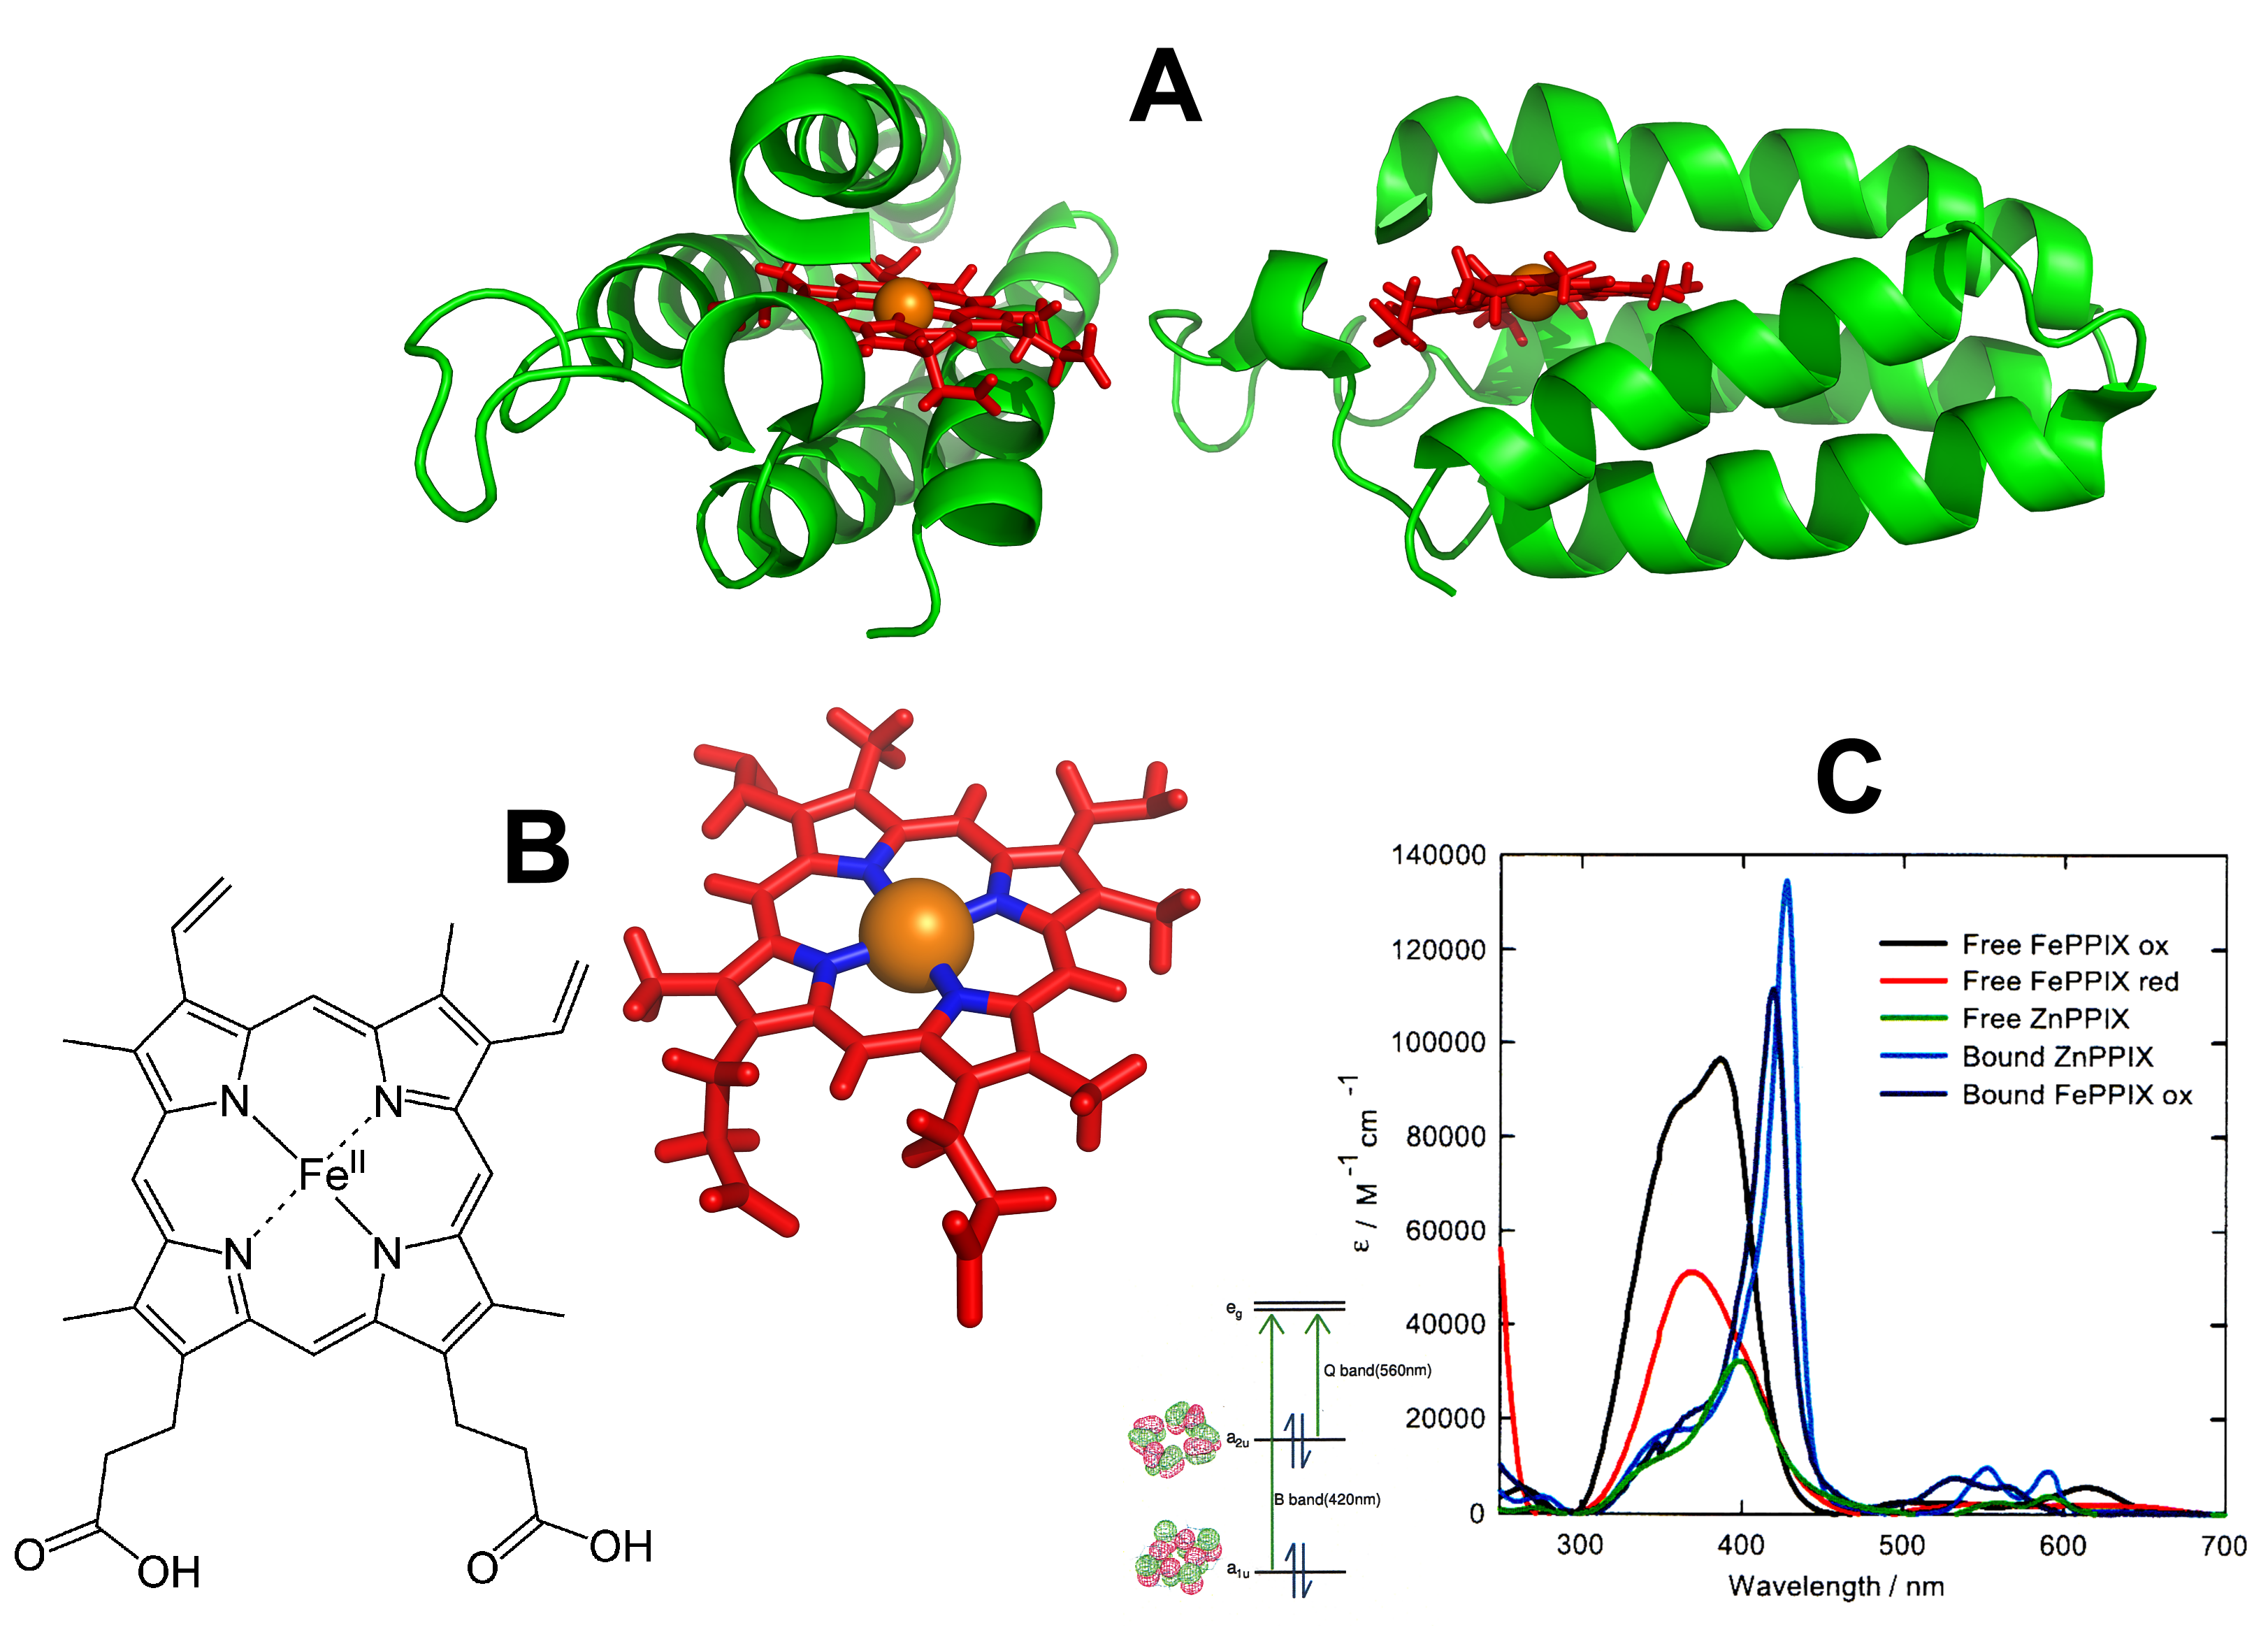
\includegraphics[width=137.4mm]{Images/haemStructure.png}
	\caption[Haem Structure]{A fancy image.}
	\label{fig:haemStructure}
\end{figure}
\end{verbatim}

\vspace{2ex}

\begin{figure}[!th]
	\centering
	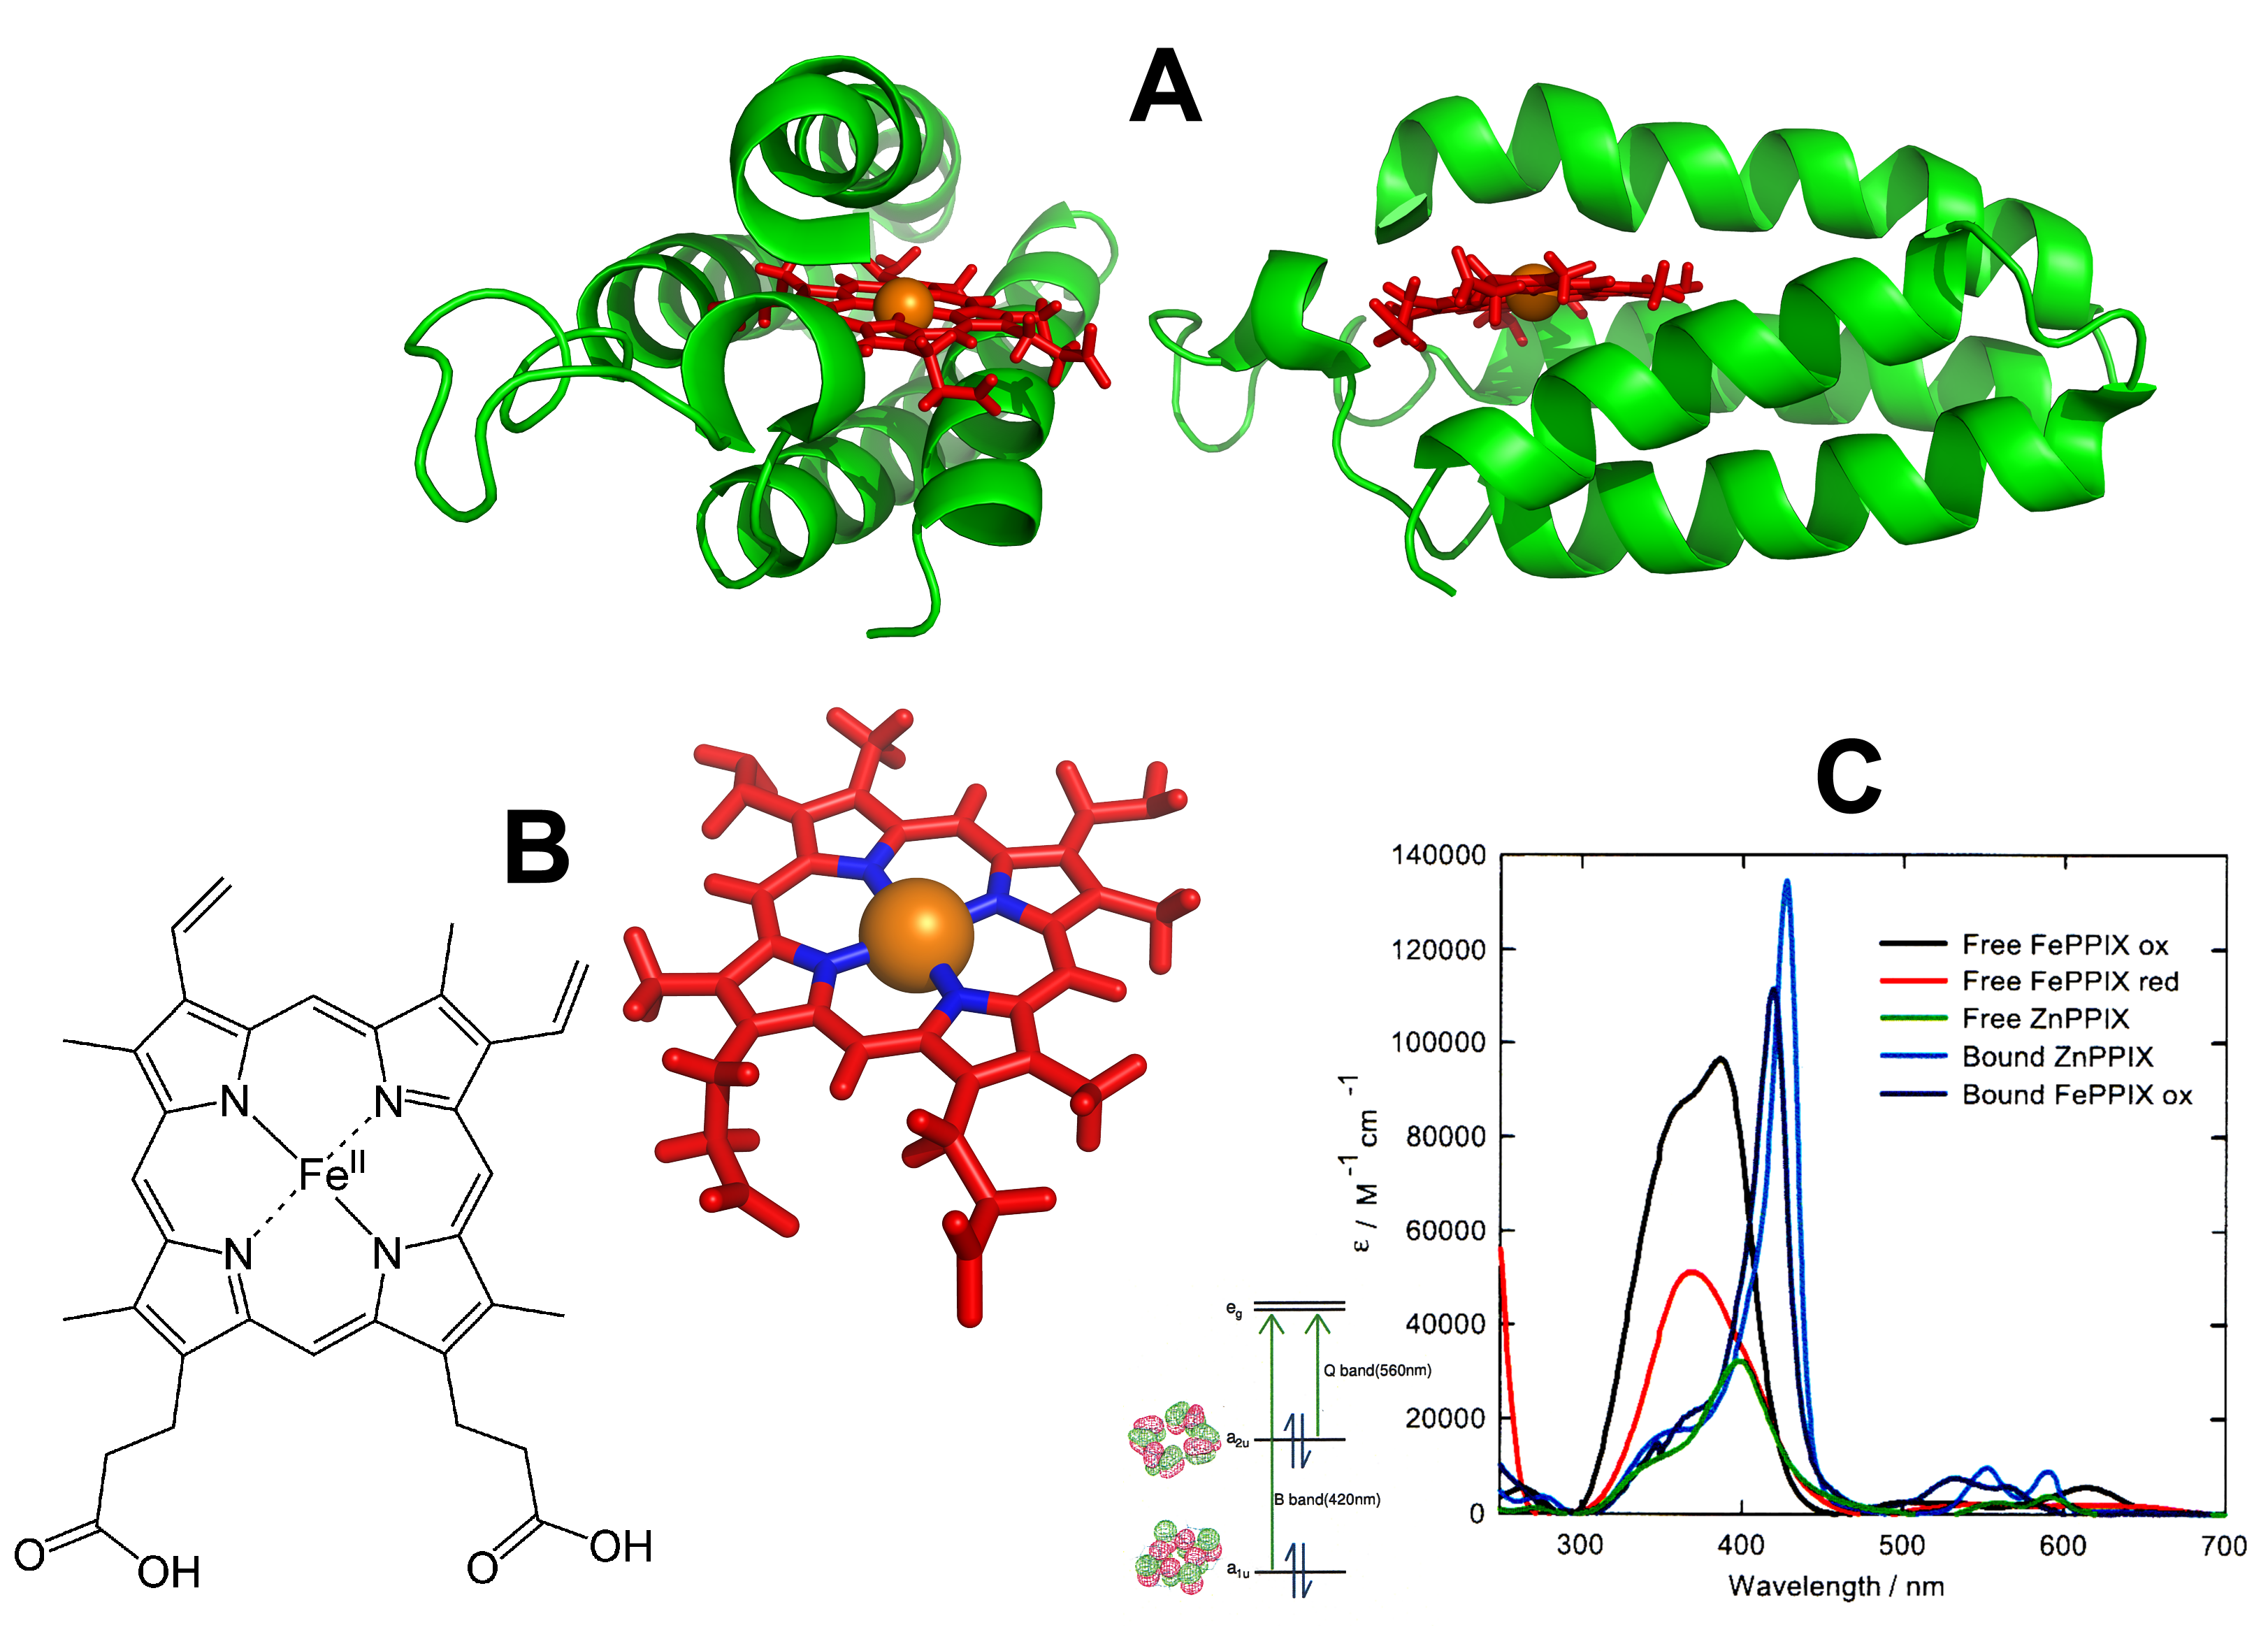
\includegraphics[width=137.4mm]{Images/haemStructure.png}
	\caption[Haem Structure]{A fancy image from Chris' Thesis.}
	\label{fig:haemStructure}
\end{figure}

In this example the command {\textbackslash}includegraphics tells LaTeX to look in the directory `Images' and incorporate the file called `haemStructure.png' into the final document while setting the width to 137.4mm.  This command can be used to resize a graphical file using the height or width parameter as shown. You must specify the units which can be pt, ex, em, mm, cm and so on. LaTeX recognises a very wide variety of standard units and graphics formats. The command is part of the graphicx package and so in the preamble you must include the command {\textbackslash}usepackage\{graphicx\}.

Many packages have been written to provide new commands. For example the `subfigure' package enables you to place separate images or files in the same figure side by side while giving them their own label. However, in this document we only concentrate on the very basics.

\section{Floating Environments}

Both tables and figures are examples of a `floating environments' which means LaTeX decides where to put them. 

The mysterious [!tbh] letters give guidance to LaTeX about roughly where the figure or table is  allowed to be, but in general they can move a long way from where you position them within your text file.  The letters in the square bracket can be t, h or b which stand for top, here or bottom.  If you don't specify any letters LaTeX defaults to [t].

LaTeX will always preserve the order in which figures appear.  If it cannot find a type setting solution, then it may move the float to it's own page, and combine it with other figures. If it still can't fit that in for some reason then it moves the float to the end of the document.  This has the effect of pushing all the remaining floating environments to the end of the document also.

The exclamation mark instructs LaTeX to ``try harder'' at putting the float where you told it to. Often you must play around to ensure the float positioning is acceptable, but usually this can be achieved by stretching or shrinking the image slightly using the size parameter, re-ordering text, judicial applications of the {\textbackslash}pagebreak command or by shouting loudly and slapping the computer monitor about. Note that it is better to resize the image using the original program that was used to create the image. Also using vector graphics can assist be useful (e.g. eps files) because they are designed to scale better.
\chapter{The Chapter on Making Chapters}
\label{sec:Chapters}

Right. LaTeX forces you to structure your document. There a series of simple commands for achieving this:

\vspace*{2ex}

{\textbackslash}chapter\{chapterName\}

{\textbackslash}section\{sectionName\}

{\textbackslash}subsection\{subsectionName\}

{\textbackslash}subsubsection\{subsubsectionName\}

\vspace*{2ex}

Easy enough. At the start of each chapter or section just issue one of these commands to name the section and LaTeX will present the chapter heading in the right style of font, which will be the same style of all the other heading names at that level of hierarchy throughout the document. In addition LaTeX assigns a number to that section. For example, this chapter was created using the command:

\vspace*{2ex}

{\textbackslash}chapter\{The Chapter on Making Chapters\} 

\vspace*{2ex}

LaTeX assigns the correct chapter number to each chapter in turn and then puts it in the table of contents, as you can see by looking at the table of contents! Easy.

\pagebreak
\section{The Section About Sections}
\label{sec:Section}
I think you're getting the hang of this. This section was created using the command {\textbackslash}section\{The Section About Sections\}. It appears in the table of contents as section \ref{sec:Section}.

\subsection{The Sub-Section About Sub-Sections}
\label{sec:SubSection}
Now you're really getting the hang of this. This subsection was created using the command {\textbackslash}subsection\{The Sub-Section About Sub-Sections\}. 

\subsubsection{The Sub-Sub-Section About Sub-Sub-Sections}
\label{sec:SubSubSection}
Now you're really getting the hang of this. but.. caught you out! This subsubsection doesn't have a number!  Ha Ha! It was created using the command {\textbackslash}subsubsection\{The Sub-Sub-Section About Sub-Sub-Sections\} in the same vein as all the other subsections/chapters etc. Here we have stopped the depth of the section numbering at the second level with the command:

\vspace*{2ex}

{\textbackslash}setcounter\{secnumdepth\}\{2\}

\vspace*{2ex}

Easy. WYSIWYM.  LaTeX does what you tell it to do. This is both a blessing and a curse.

\pagebreak
\section*{The Section About Sections That Don't Appear in the Table of Contents}
\label{sec:InvisibleSection}
Ok. Now we're throwing a spanner in the works. This section was created using the command:

\vspace*{2ex}

{\textbackslash}section*\{The Section About Sections That Don't Appear in the Table of Contents\}. 

\vspace*{2ex}

Notice how LaTeX has not assigned a number to the section and it doesn't appear in the table of contents. The effect of the * is to suppress the inclusion of a chapter, section or subsection in the automatic numbering. Easy. You can do this at any level. This is useful for things like prefaces, tables of contents or acknowledgements which you may or may not wish to have an entry in the main contents table. Up to you. It's your thesis. Don't just copy me.

\section{A Small Point About Numbering}

In this section notice how the numbering starts from where it left off before we suppressed the numbering on the previous section. Easy. WYSIWYM.
\pagebreak
\section{The Section About Internal Referencing}
\label{sec:InternalReferencing}

There are two related commands:

\vspace*{2ex}

{\textbackslash}label\{labelName\} 

{\textbackslash}ref\{labelName\}

\vspace*{2ex}


The {\textbackslash}label\{\} command allows you to create a label in a particular environment\footnote{That's right. Chapters, Sections and sub-sections etc are environments!}. The label won't appear in the final document. It's just a label which makes it easy to refer back to any particular environment elsewhere in the document. The {\textbackslash}ref\{\} command enables you to insert a reference anywhere in the document to any label in the document.  For example this is section \ref{sec:InternalReferencing}. The names you use in a label can be anything you like but musn't contain whitespace or special characters. I used the two commands:

\vspace*{2ex}

{\textbackslash}label\{sec:InternalReferencing\}

{\textbackslash}ref\{sec:InternalReferencing\}.

\vspace*{2ex}

The astute among you will realise that LaTeX has to read the document several times. Once to find the labels and then again to populate the references with the correct numbers. So you have to compile a latex document twice to get the referencing right. If there is a missing label or you refer to something that doesn't exist then latex inserts a convenient ? at that point. So hunting for queries is useful way of finding broken references. Latex issues warnings when it finds broken references.

As you create a document you will find yourself putting labels in all over the place so choose a sensible naming convention to help you remember the label names.

Each type of environment (equations, figures, tables, sections etc) has its own independent numbering system.  So when you choose your label name it's a good idea to have an identifier for that type of environment.  I have my own convention for label names which I use to help me remember references. E.g.   sec:SectionAboutCats. Eqn:EquationAboutCats,  Fig:FigureAboutCats and so on. This means you can differentiate between referring to the section or the figure more easily, even though they are about the same thing.

So Internal Referencing is a doddle. Easy!
\chapter{Organising Your Files}
One of the drawbacks of word is that the figures and tables are included within the document which becomes very very clunky quite quickly and once it reaches around 100Mb it becomes unwieldy and hard to export. One of that advantages of LaTeX is that the files are all text files and so are very light on resources and are easy to email around the place.

However, sometimes it can be difficult to navigate through a single text file, so if you had a huge document then it becomes difficult to find your way around.  One way of circumnavigating this problem is to break the file up into smaller files. As long as LaTeX knows where to look you can have a file for each logical sub-division of your document.

Therefore it is worth spending a bit of time at the beginning of a large project deciding how you wish to break up your LaTex Files and organise them neatly and tidily.  You can then tell LaTex where to look for the files using the following command:

\vspace*{2ex}
{\textbackslash}include\{fileName\}
\vspace*{2ex}

\pagebreak
\section{Linking a File}
We are now going to copy part of the tutorial file into a separate files and link it the main file.  Because this could go wrong it is sensible to back up tutorial.tex as something else. So save a copy called `tutorialOriginal.tex' for safe keeping. Then follow the following instructions.

\begin{enumerate}
\item Create a new file called MyFirstPage.tex
\item Select and Cut out the first chapter of Tutorial.Tex
\item Paste the first chapter into MyFirstPage.tex
\item Save both tutorial.tex and MyFirstPage.tex
\item Then add {\textbackslash}include\{MyFirstPage\} in tutorial.tex where the text used to be before you cut it out. We don't need to add the `.tex' because LaTeX can only include `.tex' files.
\item compile tutorial.tex and view the PDF
\end{enumerate}

The final PDF should look exactly the same as it was! except we now have a separate file for one of the chapters.

\pagebreak
\section{Creating A Class File}
We can also save our preamble in a separate file called a class file. This makes your main document much easier to understand.  To make it work we need to use the {\textbackslash}LoadClass\{\} command as follows: 

\begin{enumerate}
\item Create another new file and save it as TutorialStyle.cls
\item Copy the preamble of tutorial.tex into the new file. Starting with the {\textbackslash}documentclass{} command and copy right up to, but not including, the {\textbackslash}begin{document} command. Delete the preamble in the original document.
\item Save TutorialStyle.cls and tutorial.tex
\item Modify the first line of TutorialStyle.cls by replacing the word `document' with the word `Load'.
\item Add a new first line of tutorial.tex to use your new style class {\textbackslash}documentclass\{TutorialStyle\}
\item Save both files.
\end{enumerate}

\subsection{Sanity Check}

The first line of TutorialStyle.cls should now be:

\begin{verbatim}
\LoadClass[12pt, oneside, a4paper]{book}
\end{verbatim}
\vspace{2ex}

The first line of tutorial.tex should be:

\begin{verbatim}
\documentClass{TutorialStyle}
\end{verbatim}
\vspace{2ex}

We have just created what is called a style file. You can use this style file as a generic preamble for other documents as well. Compile tutorial.tex.  Nothing should have changed in the final PDF.


\pagebreak
\section{The Structure of this Document}

Lets now look at how I've organised this document. It is identical to my thesis because it started out life as my thesis. I usurped the structure and simply replaced the headings and content to make a kind of reference manual for this introductory course. This document therefore is three things:

\begin{enumerate}
\item An example thesis structure to work from.
\item The LaTeX files which were used to create it can be used as a template for a thesis.
\item It is also a convenient introductory latex manual!
\end{enumerate}

\vspace*{2ex}
Groovy huh?

\section{The Master File}

There is a master file where LaTeX begins the compilation procedure. This contains the {\textbackslash}documentclass command needed to set the ball rolling. Within the file there are a series of {\textbackslash}include\{\} commands, one for each Chapter, which tell LaTeX where to find the files containing each chapter.

The subfiles cannot be compiled on their own because they do not contain the {\textbackslash}documentclass, {\textbackslash}begin\{document\} or {\textbackslash}end\{document\} commands. Lets us look in more detail at the master file and we will learn some new LaTeX commands.

\singlespacing
\pagebreak
\begin{verbatim}
\documentclass{Style/LatexCourseStyle}

\begin{document}
\setcounter{secnumdepth}{2}
\setcounter{tocdepth}{1}

\frontmatter
\onehalfspacing
\thispagestyle{empty}

\begin{center}
\vspace*{\stretch{1}}

\hrule height 2pt
\vspace*{2ex}
{\Huge\textbf{Towards the Ability to Make Super Duper LaTeX Documents}\par}
\vspace*{2ex}
\hrule height 2pt
\vspace*{10ex}
{
\includegraphics[height=40mm]{Images/UnivShield}\par}
\vspace*{10ex}
{\large\textbf{Christopher~James~Forman}\par}
\vspace*{2ex}
{\large{Department Of Chemistry}\par}
\vspace*{2ex}
{\large{University of Cambridge}\par}
\vspace*{5ex}
{\large{This dissertation is submitted for the degree of \textit{Doctor of Philosophy}}\par}
\vspace*{5ex}
{\large{\today}\par}

\vspace*{\stretch{2}}
\end{center}
\chapter*{Declaration}

\vfill

This dissertation is the result of my own work and includes nothing which is the outcome of work done in collaboration except where specifically indicated in the text. It is not substantially the same as any that I have submitted for a degree or diploma or other qualification at any other University and no part has already been, or is concurrently being, submitted for any degree, diploma, or other qualification. It does not exceed 60,000 words, including tables, footnotes, bibliography and appendices.\par

\vspace{10ex}

\begin{flushright}
Signature: \rule[0pt]{60mm}{0.5pt}

\vspace{5ex}

Date: \rule[0pt]{60mm}{0.5pt}
\end{flushright}

\vfill
\chapter*{Acknowledgments}
\subsection*{Family}
Mum. Dad. Pet Dog.

\subsection*{Scientific Collaborations}
Dr A.N.Other at uni of blah for samples and instrument time etc. My Amazing Lab Chums.

\subsection*{Scientific Support}
My amazing lab chums.

\subsection*{General Assistance}
Cleaner, My amazing lab chums.

\subsection*{Financial Support}
Bank, Tax payer. My amazing lab chums.

\subsection*{Moral Support}
My Amazing Lab chums.

\subsection*{Academic Inspiration}
Netwon, My super. My Amazing Lab Chums.

\subsection*{Everyone else}
My Amazing Lab Chums.

\chapter*{Summary}
This document is a handbook for introducing you to LaTeX. It contains a bit of background about the history and philosophy of LaTeX.  However, it concentrates on providing a guided practical introduction to the basic techniques such as 
\begin{itemize}
\item Lists
\item Mathematical and chemical equations
\item Tables
\item Figures
\item Chapters and Sections
\item Linking to other files in large documents
\item Referencing
\end{itemize}

The handbook is also presented in the style of a thesis. This means that source files provided on the introductory course and available from the department web page are a convenient template for a thesis.

More details on specific aspects of LaTeX can be found at the departmental LaTeX page which can be found here:

 http://www-ch-int.ch.private.cam.ac.uk/latex/about

\chapter*{Abbreviations}

\begin{longtable}{r >{\rule{0pt}{3ex}}l<{\rule[-1.5ex]{0pt}{0pt}}}
ADP & Adenosine Diphosphate\\
(nc/c)AFM & (non-contact/conducting) Atomic Force Microscopy\\
ATP & Adenosine Triphosphate \\
\end{longtable}
\tableofcontents
\listoftables
\listoffigures

\mainmatter
\renewcommand{\sectionmark}[1]{\markright{\thesection \ #1}{}}
\chapter{Overview}
\label{chap:overview}
\section{LaTeX: The answer to everything.}
LaTeX is typsetting program that takes an input file of marked up text and then, with a user defined set of rules, typesets a beautifully crafted output file that can be easily printed (e.g. a pdf). 

\subsection{Advantages}

The advantages of this method are manifold:

\begin{itemize}

\item Use any text editor to view the source document.
\item More time can be spent working on the content and not worrying about how text or figures interact in the layout until later on.
\item LaTeX uses consistent rules throughout a document
\item LaTeX sorts out basic typesetting automatically
\item Changes can be introduced globally with very little effort
\item Document structure is explicit
\item Documents can be professionally typeset and look great
\item You are forced to structure your documents correctly.
\item Mathematical equations, like $E=mc^2$ or $\imath\hbar\frac{\partial}{\partial t}\Phi (x, t) = \hat{H}\Phi (x, t)$ can be produced almost as fast as typing (if you know the commands!).
\end{itemize}

\subsection{Disadvantages}
The disadvanatges of this method are also manifold:
\begin{itemize}
\item You don't see the output as you go.
\item Steep learning curve.
\item Documents are harder to edit by a second author (unless they are adept at LaTeX too). This can be mitigated using version control, which makes group authoring processes superior to word.
\item The program never works quite the way you want it to and learning how to influence it can be problematic and subtle.
\item Although intended to save work the principle of 'conservation of work' means that you simply transform problems associated with WYSISYG approaches to problems associated with WYSIWYM approaches!
\item You can go blind trying to determine the difference between wiggly and smooth brackets if your editors font isn't large enough.
\end{itemize}

\subsection{On balance?}
If it's so rubbish, why use LaTeX?

\begin{itemize}
\item Large documents are much more easily handled. 
\item In general it is quicker to debug a LaTeX document than typeset an entire thesis manually. 
\item Technical information such as tables, equations and figures are integrated much more smoothly than with word.
\end{itemize}

\section{How does it work?}

The raw text is interspersed with commands, preceded by a \textbackslash, which tell LaTeX what to do with the text. For example you can \textbf{make it bold}, \emph{italic}, or \underline{underlined} with the commands {\textbackslash}textbf\{\}, {\textbackslash}emph\{\} or {\textbackslash}underlined\{\}. More on commands in a moment...



\chapter{My First Page}

\section{The Very Beginning}
The very simplest LaTeX document might look like this:

\begin{verbatim}
\documentclass[a4paper,12pt]{article}
\begin{document}
Hello World.
\end{document}
\end{verbatim}

\pagebreak
\thispagestyle{empty}
Hello World.
\pagebreak
\subsection{Break Down}
What's all the gobbledegook around my simple message???

In LaTeX we intersperse text and commands.  Commands are preceded by a \textbackslash. For example the first line in a LaTeX document \underline{\textbf{\emph{must}}} be:

\begin{verbatim}
\documentclass[options]{class}
\end{verbatim}

Where the word ''class'' may be substituted for one of many things such as: article, proc, minimal, report, book, letter, memoir, slides, beamer.

Similarly, and completely generally in LaTeX speak, the square brackets denote the existence of optional parameters. Each individual command can take its own parameters and for the ''{\textbackslash}documentclass'' command there are options for controlling font size, font family, landscape, oneside, twosided, page size and so on. These options will persist throughout the entire document. For example the document class command for this document, (which is likely to be like the one you would use for a thesis), would be:

\begin{verbatim}
\documentclass[12pt, oneside, a4paper]{book}
\end{verbatim}

Other options include:

\begin{itemize}
\item {10pt, 11pt, 12pt (default is 10pt).}
\item {letterpaper, legalpaper, a4paper, executivepaper, a5paper, b5paper}
\end{itemize}
and so on.

\pagebreak
\section{Can I start typing please?}

After we have set up the document we can start actual work on our document. So we must tell LaTeX that what follows is to be interpreted as a document.  The command {\textbackslash}begin can take many different parameters and is a command to enter what is known, in LaTeX speak, as 'an environment'. Thus the commands:
\begin{verbatim}
\begin{document}

\end{document}
\end{verbatim}

tells LaTeX to enter and leave the document environment, and thus constitute the outer limits of our document file. Other environments include the equation environment, the itemize environment, the figure environment and so on. These will be encountered in due course.

Every part of the LaTeX file is therefore within an environment of specific type and the content within each environment consists of commands or text.

That's basically it.

So let's get on with it shall we...

\pagebreak
\section{The ground rules}
\begin{quote}
Hold on, hold on, hold on my son.

First the lessons.

Then the fun!
\end{quote}
Dr Seuss.

\subsection{Spaces}
Whitespace characters, such as blank or tab, are treated uniformly as space by LaTeX. Several consecutive whitespace characters are treated as one single space. Whitespace at the start of a line is generally ignored, and a single line break is treated as whitespace. An empty line between two lines of text defines the end of a paragraph. Several empty lines are treated the same as one empty line. The text below is an example.

\begin{verbatim}
It does not matter whether you
enter one or several             spaces
after a word. The final result will be typeset beautifully
according    to     precise rules.




An empty line starts a new
paragraph. Note the indentation on the first line of the paragraph, 
except at the beginning of the section. 
\end{verbatim}

\vspace*{2ex}
\vspace*{2ex}

It does not matter whether you
enter one or several             spaces
after a word. The final result will be typeset beautifully
according    to     specific rules.




An empty line starts a new
paragraph. Note the indentation on the first line of the paragraph, except at the beginning of the section. 

\pagebreak
\subsection{Special Characters}
The symbols 

\# \$ \% \textasciicircum{} \& \_ \{ \} \~{} \textbackslash

are reserved characters that either have a special meaning under LaTeX or are unavailable in all the fonts. If you enter them directly in your text, they will normally not print, but rather make LaTeX do strange things.

To overide the special meanings of these symbols and allow them to produced within your text you may use the following sequences:
\begin{verbatim}
\# \$ \% \textasciicircum{} \& \_ \{ \} \~{} \textbackslash
\end{verbatim}

Other symbols and many more can be printed with special commands in mathematical formulae or as accents.

The backslash character '\textbackslash' cannot be entered by adding another backslash in front of it ( \textbackslash\textbackslash); because this sequence means ''linebreak''.

The command \textbackslash\~{}\{\} produces a tilde which is placed over the next letter. For example \textbackslash\~{}\{n\} gives \~{n}. To produce just the character \~{}, use \textbackslash\~{}\{\} which places a \~{} over an empty box.

Similarly, the command \textbackslash\textasciicircum{} produces a hat over the next character, for example \textbackslash\textasciicircum\{o\} produces \^{o}.

\pagebreak
\section{Preamble}
After the {\textbackslash}documentclass command we add ''preamble''. Here we load special features that we will use throughout our document to expand on the basic capabilities of LaTex. These are contained in units called ''packages'' which we can tell our LaTeX compiler to download by using the command ''{\textbackslash}include\{packageName\}''. 

There are many repositories of such packages on the web. Your compiler generally knows where to look and most standard packages are included with any install. For example, to include a special set of typesetting instructions to handle chemical equations we can grow our simple document with a single command like this:

\begin{verbatim}
\documentclass[a4paper,12pt]{article}
\usepackage[version=3]{mhchem}
\begin{document}
Hello World!

We all need \ce{H2O}.

I'm less fussed about \ce{^{235}_{92}U+}.

\end{document}
\end{verbatim}

\vspace{2ex}

\pagebreak
\thispagestyle{empty}
Hello World!

We all need \ce{H2O}.

I'm less fussed about \ce{^{235}_{92}U+}.
\pagebreak

Here we have loaded a package called: "`mhchem"' which took the option ''[version=3]''. This is a package for drawing chemical equations easily and it has it's own instruction manual which you can follow easily. It is included in the bundle of files for this course.

Other things we can do in the premable within LaTeX are to redefine existing commands or create our own personal commands. These can be stored in a file called the 'style file' which we can load at the beginning of our document, in place of our documentclass. More about this later on...


\subsection{Comments}
It is often useful to comment your LaTeX documents. You can leave yourself amusing, sarcastic messages that won't get printed out in the final document. Use this to make your own notes as the course progresses.

To get a comment use the \% command, which tells LaTeX to ignore the rest of the line, the line break and all the white space at the beginning of the next line, for example, we may add to our continually evolving document...

\begin{verbatim}
\documentclass[a4paper,12pt]{article}
\usepackage[version=3]{mhchem}
\begin{document}
Hello World!

%All humans need water and I would like 
%to include this concept in my arguments.
We all need \ce{H2O}.

%Uranium 235 is toxic, which is why I don't want to consume it... 
I'm less fussed about \ce{^{235}_{92}U+}.

\end{document}
\end{verbatim}

\vspace{4ex}
Hello World!

%All humans need water and I would like to include this concept in my arguments.
We all need \ce{H2O}.

%Uranium 235 is toxic, which is why I don't want to consume it... 
I'm less fussed about \ce{^{235}_{92}U+}.

\pagebreak
\section{Compiling}
Once the document is finished you can compile it. Your compiler will depend on the platform that you use. In the PWF we are using winEDT to edit the documents (a LaTeX front end) and texlive2008 which is the compiler itself. I use MiKTex and the front end texCenter.  There is no need to use a front end. If you prefer you can use a simple text editor and a command line.

the recommended distributions are:
\begin{itemize}
\item MiKTeX or TeX Live for Windows
\item TeX Live for Unix/Linux
\item MacTeX or TeX Live for Mac OS.
\end{itemize}

Once you have installed your software and got it working, written your source code and tried to compile it, there will nearly always be something wrong with your file. 

Any errors will be highlighted in the console window or error output box of your front end.  Some front ends dump the running commentary which LaTeX produces into a text file for easy reading afterwards.

In a compile attempt (successful or otherwise) LaTeX may produce the following files:

projectname.aux

projectname.bbl

projectname.lof

projectname.lot

projectname.txt

projectname.toc

projectname.dvi

These are interim files (toc= table of contents, bbl = bibliography etc). To be honest I have no idea what half of these things contain.  You only need the .tex file and a compiler with the right packages installed to produce them again.

Some versions of LaTeX only produce DVI files and you then need to convert the dvi file to a PDF or download a dvi viewer. You can also convert DVI files to PS files and then view them.  The good thing about front ends is that you can set them up to produce PDFs directly.

OK. So we have now produced a silly document but we understand it.  Now lets get on with learning how to make our own documents.



\chapter{Lists}
Lists are great.  The command {\textbackslash}begin\{\} can be used to enter a list environment.  For example:

\begin{verbatim}
\begin{itemize}
\item cat
\item dog
\item horse
\end{itemize}
\end{verbatim}

Produces:

\begin{itemize}
\item cat
\item dog
\item horse
\end{itemize}

\pagebreak
We can also replace the bullet points with numbers using the enumerate keyword.

\begin{verbatim}
\begin{enumerate}
\item cat
\item dog
\item horse
\end{enumerate}
\end{verbatim}

\begin{enumerate}
\item cat
\item dog
\item horse
\end{enumerate}

\pagebreak
and we can use the description keyword which does this:
\begin{verbatim}
\begin{description}
\item[Cat] a lovely furry creature with a cute nose and whiskers.
\item[Dog] Another furry creature that smells rather well; 
           its olfactory power stems from its nasal dampness.
\item [Horse] A large stinky creature with sideways facing eyes.
\end{description}
\end{verbatim}

\begin{description}
\item[Cat] a lovely furry creature with a cute nose and whiskers.
\item[Dog] Another furry creature that smells rather well; its olfactory power stems from its nasal dampness.
\item [Horse] A large stinky creature with sideways facing eyes.
\end{description}
\chapter{Maths Equations}

\section{Producing Beautiful Looking Mathematics}

One of the best features about LaTeX is `maths mode'.  For example the schrodinger equation can be produced as follows:

\vspace*{2ex}

\begin{center}
\begin{math}
\imath\hbar\frac{\partial}{\partial t}\Phi (x, t) = \hat{H}\Phi (x, t)
\end{math}
\end{center}

\vspace*{2ex}

\begin{verbatim}
\begin{math}
\imath\hbar\frac{\partial}{\partial t}\Phi(x,t)=\hat{H}\Phi(x,t)
\end{math}
\end{verbatim}

There are a number of ways to switch on maths mode.  The first, as above, is with the {\textbackslash}begin\{math\} environment. You can also enter mathmode inline using the \$ symbol. For example typing in \$y=ax\textasciicircum{}2+bx+c\$ yields $y=ax^2+bx+c$.  Another way is to enter the equation environment which enables you to number equations so you can then refer to them later in the text.

\begin{equation}
y(t)= \sin \left(\frac{{\alpha}t}{2\pi} + \phi_0\right)
\label{eqn:MadeUpNonsense}
\end{equation}

\vspace*{2ex}
\begin{verbatim}
\begin{equation}
y(t)= \sin \left(\frac{{\alpha}t}{2\pi} + \phi_0\right)
\end{equation}
\end{verbatim}.

\section{Basic Maths Mode}
Once in maths mode there is a kind of text based code for writing down your equations.  Here are the most basic symbols to get you going.
\begin{center}
\begin{tabular}{cc}
\toprule
Final Result & LaTeX Code \\
\cmidrule(){1-2}
$a+b$ & a+b \\
$a-b$ & a-b \\
$ab$ & ab \\
$a*b$ & a*b \\
$a \times b$ & a {\textbackslash}times b \\
$a \cdot b$ & a {\textbackslash}cdot b \\
$\frac{a}{b}$ & {\textbackslash}frac\{a\}\{b\} \\ 
$a^b$ & a\textasciicircum{}b \\
$a_b$ & a\_b \\
$\sin a$ & {\textbackslash}sin a  (same for cos, tan)\\
$ sin a$ & sin a \\
$\sqrt{a}$ & {\textbackslash}sqrt\{a\} \\
$\left( a \right) $ & {\textbackslash}left( a {\textbackslash}right)\\ 
$\left[ a \right]$ & {\textbackslash}left[ a {\textbackslash}right]\\ 
$\alpha$ & {\textbackslash}alpha \\
$\pi$ & {\textbackslash}pi \\
\bottomrule
\end{tabular}
\end{center}

A full treatise on maths mode is not practical here. There are lots of online tutorials and summaries of symbols. It just takes a bit of practice and you can build up equations really easily. It's straight forward to learn new stuff once you've done it a few times.

\pagebreak
\section{Equation Arrays}
Sometimes you need to arrange several equations vertically, referencing individual lines separately and aligning the equations on the $=$ sign. This can be achieved with equation arrays as follows:

\begin{eqnarray}
A\left( x\right) & = & \frac{x^2+2x+1}{x+1} \\
& = & \frac{\left(x+1\right)\left(x+1\right)}{x+1} \nonumber\\
& = & x+1 \nonumber\\
B(x,t) & = & \frac{e^{\left(\imath\omega_0 t + kx\right)}}{4\pi\epsilon_0}
\end{eqnarray}

\begin{verbatim}
\begin{eqnarray}
A\left( x\right) & = & \frac{x^2+2x+1}{1+x} \\
& = & \frac{\left(x+1\right)\left(x+1\right)}{1+x} \nonumber\\
& = & x+1 \nonumber\\
B(x,t) & = & \frac{e^{\left(\imath\omega_0 t + kx\right)}}{4\pi\epsilon_0}
\end{eqnarray}
\end{verbatim}

\begin{itemize}
\item Note the \& symbols. This tells LaTeX where to align the equations. There must be the same number of \& symbols in each line.
\item Note the \textbackslash\textbackslash ~at the end of each line except the last one. This symbol tells LaTeX to add another row in the array.  If you put it on the last line you get an empty row at the bottom of the array.
\item Note the {\textbackslash}nonumber command which suppresses line numbering for that line.
\item Note that equation number carries on from equation \ref{eqn:MadeUpNonsense} in the previous section.
\end{itemize}

\section{Maths Packages}

Maths mode comes as standard in LaTeX, however you can download packages that buff up your maths symbol set. For example neat vector notation comes in the package `vector'. e.g. {\textbackslash}uuvec\{T\} yields $\uuvec{T}$.

\begin{verbatim}
\usepackage{amssymb}
\usepackage{amsmath}
\usepackage{vector}
\end{verbatim}


\chapter{Chemical Equations}
The mhchem package means you can do basic stuff very easily using {\textbackslash}ce\{\}. For example:

\vspace{2ex}
\begin{verbatim}
\ce{CO2 + C -> 2CO}
\ce{CO2 + C <- 2CO}
\ce{CO2 + C <=> 2CO}
\ce{A-B=C#D\sbond E\dbond F\tbond G}
\end{verbatim}
\vspace{2ex}
\begin{center}
\ce{CO2 + C -> 2CO}

\ce{CO2 + C <- 2CO}

\ce{CO2 + C <=> 2CO}

\ce{A-B=C#D\sbond E\dbond F\tbond G}
\end{center}

\vspace{2ex}
You can also use math mode within chemical equations.
\vspace{2ex}

\begin{center}
\ce{$x\,$ Na(NH4)HPO4 ->[\Delta] (NaPO3)_{$x$} + $x\,$ NH3 ^ + $x\,$ H2O}
\end{center}

\begin{verbatim}
\ce{$x\,$ Na(NH4)HPO4 ->[\Delta](NaPO3)_{$x$} + $x\,$ NH3 ^ + $x\,$ H2O}
\end{verbatim}

And you can number chemical reactions as well by using the math mode equation environment.

\begin{equation}
\ce{CO2 + C <=> 2CO}
\end{equation}

\begin{verbatim}
\begin{equation}
\ce{CO2 + C <=> 2CO}
\end{equation}
\end{verbatim}

However, this will number mathematical and chemical equations using the same number system. There is a discussion in the mhchem pdf which shows you how to number chemical and mathematical equations independently. It's a bit complex and involves you creating your own type of environment... bit beyond the intro level of this course...
\chapter{Tables}
Tables are big business in Latex.  I use these packages to help me.

\begin{verbatim}
\usepackage{multirow}
\usepackage{booktabs}
\usepackage{dcolumn}
\end{verbatim}

Here's an example table

\begin{table}[!hb]
 \centering
	\begin{tabular}{@{}rccc@{~}r@{.}l*3{r@{.}l@{~}r@{.}l}D{.}{\cdot}{2,1}}
	\toprule
	\multicolumn{1}{c}{Fibre Type}
	& N 
	& M 
	&\multicolumn{3}{c}{$L_t$ (nm)}
	&\multicolumn{4}{c}{$R_t$ (nm)}
	&\multicolumn{4}{c}{$d_t$ (nm)}
	&\multicolumn{4}{c}{${\Delta}Z_t$ (nm)}
	&\multicolumn{1}{c}{~}\\
\cmidrule(lr){1-1}
\cmidrule(lr){2-2}
\cmidrule(lr){3-3}
\cmidrule(lr){4-6}
\cmidrule(lr){7-10}
\cmidrule(lr){11-14}
\cmidrule(lr){15-18}
  SS Twisted & 5 & 4 & 313 &\multicolumn{2}{c}{(122)} & 5&7 &(1&6)  & 5&4 &(1&0)  &  150&5 &(63&1) &\multicolumn{1}{c}{~} \\
  \multicolumn{19}{c}{~}\\
  %\cmidrule(lr){3-18}
  &
  &
 	&\multicolumn{3}{c}{$L_s$ (nm)} 
 	&\multicolumn{4}{c}{$R_s$ (nm)}
 	&\multicolumn{4}{c}{$W_s$ (nm)}
 	&\multicolumn{4}{c}{${\Delta}Z_s$ (nm)}
 	&\multicolumn{1}{c}{${\Delta}Z_{e}$ (nm)}\\
\cmidrule(lr){4-6}
\cmidrule(lr){7-10}
\cmidrule(lr){11-14}
\cmidrule(lr){15-18}
\cmidrule(lr){19-19}
  SS Spiral& 32 & 7 &123&(31&6)&11&4&(3&3)&11&1&(2&6)&32&9&(22&2)&26.9\\
  SSB Spiral& 64&18 &106&(22&9)&10&8&(2&7)&9&8&(1&8)&28&2&(8&1)&22.7\\
	%\midrule
  BSS Spiral&37 &19 &110&(44&9)&13&4&(3&0)&12&9&(1&8)&27&1&(9&1)&21.5\\
	%\midrule
  SSSB Spiral&26& 6 &104&(23&9)&13&3&(2&6)&16&4&(3&4)&29&9&(11&1)&22.5\\
	\bottomrule
	\end{tabular}	
	\caption[Basic Fibre Dimensions by TEM]{A funky table from my thesis.}
	\label{tab:BasicXSBFibreDimensionsTEM}
\end{table}

\pagebreak
Here's what the code looks like:
\begin{verbatim}
\begin{table}[!hb]
 \centering
	\begin{tabular}{@{}rccc@{~}r@{.}l*3{r@{.}l@{~}r@{.}l}D{.}{\cdot}{2,1}}
	\toprule
	\multicolumn{1}{c}{Fibre Type}
	& N 
	& M 
	&\multicolumn{3}{c}{$L_t$ (nm)}
	&\multicolumn{4}{c}{$R_t$ (nm)}
	&\multicolumn{4}{c}{$d_t$ (nm)}
	&\multicolumn{4}{c}{${\Delta}Z_t$ (nm)}
	&\multicolumn{1}{c}{~}\\
\cmidrule(lr){1-1}
\cmidrule(lr){2-2}
\cmidrule(lr){3-3}
\cmidrule(lr){4-6}
\cmidrule(lr){7-10}
\cmidrule(lr){11-14}
\cmidrule(lr){15-18}
  SS Twisted & 5 & 4 & 313 &\multicolumn{2}{c}{(122)} & 5&7 &(1&6)  & 5&4 &(1&0)  &  150&5 &(63&1) &\multicolumn{1}{c}{~} \\
  \multicolumn{19}{c}{~}\\
  %\cmidrule(lr){3-18}
  &
  &
 	&\multicolumn{3}{c}{$L_s$ (nm)} 
 	&\multicolumn{4}{c}{$R_s$ (nm)}
 	&\multicolumn{4}{c}{$W_s$ (nm)}
 	&\multicolumn{4}{c}{${\Delta}Z_s$ (nm)}
 	&\multicolumn{1}{c}{${\Delta}Z_{e}$ (nm)}\\
\cmidrule(lr){4-6}
\cmidrule(lr){7-10}
\cmidrule(lr){11-14}
\cmidrule(lr){15-18}
\cmidrule(lr){19-19}
  SS Spiral& 32 & 7 &123&(31&6)&11&4&(3&3)&11&1&(2&6)&32&9&(22&2)&26.9\\
  SSB Spiral& 64&18 &106&(22&9)&10&8&(2&7)&9&8&(1&8)&28&2&(8&1)&22.7\\
	%\midrule
  BSS Spiral&37 &19 &110&(44&9)&13&4&(3&0)&12&9&(1&8)&27&1&(9&1)&21.5\\
	%\midrule
  SSSB Spiral&26& 6 &104&(23&9)&13&3&(2&6)&16&4&(3&4)&29&9&(11&1)&22.5\\
	\bottomrule
	\end{tabular}	
	\caption[Basic Fibre Dimensions by TEM]{A funky table from my thesis.}
	\label{tab:BasicXSBFibreDimensionsTEM}
\end{table}
\end{verbatim}

\pagebreak

\section{Tables Made Easy}
Here is a simple table followed by the code that produced it.

\begin{center}
\begin{tabular}{lcr}
anchovy & banana & carrot \\
dog & apple & fennel \\
goat & strawberry & potato
\end{tabular}

\vspace*{2ex}

\begin{verbatim}
\begin{tabular}{lcr}
anchovy & banana & carrot \\
dog & apple & fennel \\
goat & strawberry & potato
\end{tabular}
\end{verbatim}
\end{center}

\vspace*{2ex}

The tabular environment is a special case of the ''array'' environment for distributing content uniformly across a region of the page.  This ability has already been exploited to align mathematical equations. For now though look at the first line.

\vspace*{2ex}

\begin{verbatim}
\begin{tabular}{lcr}
\end{verbatim}

\vspace*{2ex}

This command tells LaTeX to enter the tabular environment. The letters l, c and r in the curly braces tell LaTeX to create a table with three columns in which the first column is left justified, the second column is centered and the third column is right justified. Lets add a fourth column and this time center justify all the columns.

\begin{center}
\begin{tabular}{cccc}
anchovy & banana & carrot & Johnny\\
dog & apple & fennel & Pete\\
goat & strawberry & potato &
\end{tabular}

\vspace*{2ex}

\begin{verbatim}
\begin{tabular}{cccc}
anchovy & banana & carrot & Johnny\\
dog & apple & fennel & Pete\\
goat & strawberry & potato &
\end{tabular}
\end{verbatim}
\end{center}

\vspace*{2ex}

Each row in the table is a list of items separated by the {\&} symbol. The end of each row is denoted by \textbackslash\textbackslash.  The last row in the table doesn't have a \textbackslash\textbackslash. You do not have to have data between the ampersands but you must have the right number of ampersands to match the number of columns that LaTeX is expecting.

\subsection{Adding Borders To Tables}
\label{sec:vertLines}
Tables should never have vertical lines. No professionally typeset table contains vertical lines. Do not put vertical lines in your tables. That said it is easy to do.

\begin{center}
\begin{tabular}{|c|c|c|c|}
anchovy & banana & carrot & Johnny\\
dog & apple & fennel & Pete\\
goat & strawberry & potato &
\end{tabular}

\vspace*{2ex}

\begin{verbatim}
\begin{tabular}{|c|c|c|c|}
anchovy & banana & carrot & Johnny\\
dog & apple & fennel & Pete\\
goat & strawberry & potato &
\end{tabular}
\end{verbatim}
\end{center}

\vspace*{2ex}

Tables should have neatly headed columns with the heading for each field separated from the data by horizontal lines. The {\textbackslash}toprule, {\textbackslash}cmidrule{} and {\textbackslash}bottomrule commands from the booktabs package are useful for controlling horizontal lines.

\begin{center}
\begin{tabular}{cccc}
\toprule
Ingredient 1 & Ingredient 2 & Ingredient 3 & Source \\
\cmidrule(){1-4}
anchovy & banana & carrot & Johnny\\
dog & apple & fennel & Pete\\
goat & strawberry & potato & \\
\bottomrule
\end{tabular}

\vspace*{2ex}

\begin{verbatim}
\begin{tabular}{cccc}
\toprule
Ingredient 1 & Ingredient 2 & Ingredient 3 & Source \\
\cmidrule(){1-4}
anchovy & banana & carrot & Johnny\\
dog & apple & fennel & Pete\\
goat & strawberry & potato & \\
\bottomrule
\end{tabular}
\end{verbatim}
\end{center}

Note that when using the {\textbackslash}bottomrule command you must add the \textbackslash\textbackslash ~symbol to the last line of data.  The last line of the table is now buried within the {\textbackslash}bottomrule command.

\pagebreak
\subsection{The {\textbackslash}cmidrule Command}
This useful and versatile command takes a bunch of options to control subtleties like only putting lines across some of the columns, or not quite making them cross the full width of the column. The (lr) option trims the left and right ends of the lines off. For example:

\begin{center}
\begin{tabular}{ccccc}
\toprule
Recipe Version & Ingredient 1 & Ingredient 2 & Ingredient 3 & Source \\
\cmidrule(lr){1-1}
\cmidrule(l){2-2}
\cmidrule(){3-3}
\cmidrule(r){4-4}
\cmidrule(lr){5-5}
10.1 & anchovy & banana & carrot & Johnny\\
1.34 & dog & apple & fennel & Pete\\
709.23 & goat & strawberry & potato & \\
\bottomrule
\end{tabular}

\vspace*{2ex}

\begin{verbatim}
\begin{tabular}{ccccc}
\toprule
Recipe Version & Ingredient 1 & Ingredient 2 & Ingredient 3 & Source \\
\cmidrule(lr){1-1}
\cmidrule(l){2-2}
\cmidrule(){3-3}
\cmidrule(r){4-4}
\cmidrule(lr){5-5}
10.1 & anchovy & banana & carrot & Johnny\\
1.34 & dog & apple & fennel & Pete\\
709.23 & goat & strawberry & potato & \\
\bottomrule
\end{tabular}
\end{verbatim}
\end{center}

\pagebreak
\subsection{Aligning Decimal Points}
Note that the decimal points don't line up in the new column ''Recipe Version'' in the previous section. There is a way round this with the DColumn package.

\begin{center}
\begin{tabular}{D{.}{\cdot}{4,4}cccc}
\toprule
Recipe Version & Ingredient 1 & Ingredient 2 & Ingredient 3 & Source \\
\cmidrule(lr){1-1}
\cmidrule(lr){2-2}
\cmidrule(lr){3-3}
\cmidrule(lr){4-4}
\cmidrule(lr){5-5}
10.1 & anchovy & banana & carrot & Johnny\\
1.34 & dog & apple & fennel & Pete\\
709.23 & goat & strawberry & potato & \\
\bottomrule
\end{tabular}

\vspace*{2ex}

\begin{verbatim}
\begin{center}
\begin{tabular}{D{.}{\cdot}{4,4}cccc}
\toprule
Recipe Version & Ingredient 1 & Ingredient 2 & Ingredient 3 & Source \\
\cmidrule(lr){1-2}
\cmidrule(lr){3-3}
\cmidrule(lr){4-4}
\cmidrule(lr){5-5}
\cmidrule(lr){6-6}
10.1 & anchovy & banana & carrot & Johnny\\
1.34 & dog & apple & fennel & Pete\\
709.23 & goat & strawberry & potato & \\
\bottomrule
\end{tabular}
\end{verbatim}
\end{center}

The DColumn package defines a new type of column which can be invoked placing a capital D in the {\textbackslash}tabular command which defines the table. If defined using a D, then the column is placed in mathmode. D takes four parameters: D\{a\}\{b\}\{c,d\} where a is the symbol which is to be aligned, b is the symbol with which to replace the aligning character, and {c,d} must be integers which indicate LaTeX should have up to c white space characters before the aligning character and d afterwards, thereby defining the position of the number within the column. The command {\textbackslash}cdot prints a special type of mathmode symbol which is a dot that is vertically shifted and larger than a normal period e.g.: $\cdot$ 

\pagebreak
\subsection{Final Table Trick}
DColumn forces the column to be in mathmode which is why the heading ''Recipe Version'' was typeset in italics in the previous section. Indeed LaTeX tried to interpret the heading of the table as a number to be aligned.  We can over ride this behaviour by using the {\textbackslash}multicolumn command to locally impose a different type of justification and temporarily disable mathmode as follows:

\begin{center}
\begin{tabular}{D{.}{\cdot}{4,4}cccc}
\toprule
\multicolumn{1}{c}{Recipe Version}& Ingredient 1 & Ingredient 2 & Ingredient 3 & Source \\
\cmidrule(lr){1-1}
\cmidrule(lr){2-2}
\cmidrule(lr){3-3}
\cmidrule(lr){4-4}
\cmidrule(lr){5-5}
10.1 & anchovy & banana & carrot & Johnny\\
1.34 & dog & apple & fennel & Pete\\
709.23 & goat & strawberry & potato & \\
\bottomrule
\end{tabular}

\vspace*{2ex}

\begin{verbatim}
\begin{tabular}{D{.}{\cdot}{4,4}cccc}
\toprule
\multicolumn{1}{c}{Recipe Version} & Ingredient 1 & Ingredient 2 & Ingredient 3 & Source \\
\cmidrule(lr){1-1}
\cmidrule(lr){2-2}
\cmidrule(lr){3-3}
\cmidrule(lr){4-4}
\cmidrule(lr){5-5}
10.1 & anchovy & banana & carrot & Johnny\\
1.34 & dog & apple & fennel & Pete\\
709.23 & goat & strawberry & potato & \\
\bottomrule
\end{tabular}
\end{verbatim}
\end{center}

This introduces you to the multicolumn command which you can use to span text over several columns.  The format is \textbackslash{multicolumn}\{n\}\{j\}\{text\} where n is the number of columns to span. j is the justification: either l,c or r and text is the text to add. There is also a similar command \textbackslash{multirow}.

\pagebreak
\section{Numbering Tables}
To tell LaTeX to assign a number to a table and add it to the list of tables you must use the {\textbackslash}begin\{table\} command to tell LaTeX to create a table environment as follows:

\begin{table}[!bh]
\centering
\begin{tabular}{D{.}{\cdot}{4,4}cccc}
\toprule
\multicolumn{1}{c}{Recipe Version}& Ingredient 1 & Ingredient 2 & Ingredient 3 & Source \\
\cmidrule(lr){1-1}
\cmidrule(lr){2-2}
\cmidrule(lr){3-3}
\cmidrule(lr){4-4}
\cmidrule(lr){5-5}
10.1 & anchovy & banana & carrot & Johnny\\
1.34 & dog & apple & fennel & Pete\\
709.23 & goat & strawberry & potato & \\
\bottomrule
\end{tabular}
\caption[Table of Banned Recipes]{Recipes that ought to be banned.}
\label{tab:Recipes}
\end{table}
\begin{verbatim}
\begin{table}[!bh]
\centering
\begin{tabular}{D{.}{\cdot}{4,4}cccc}
\toprule
\multicolumn{1}{c}{Recipe Version}& Ingredient 1 & Ingredient 2 & Ingredient 3 & Source \\
\cmidrule(lr){1-1}
\cmidrule(lr){2-2}
\cmidrule(lr){3-3}
\cmidrule(lr){4-4}
\cmidrule(lr){5-5}
10.1 & anchovy & banana & carrot & Johnny\\
1.34 & dog & apple & fennel & Pete\\
709.23 & goat & strawberry & potato & \\
\bottomrule
\end{tabular}
\caption[Table of Banned Recipes]{Recipes that ought to be banned.}
\label{tab:Recipes}
\end{table}
\end{verbatim}

In the table environment the {\textbackslash}caption[text1]\{text2\} command adds a caption, where text1 appears in the list of tables at the beginning of the document and text2 is the local caption.  The label command creates a label with which to reference the table e.g. Table \ref{tab:Recipes} is a table of recipes that have been made up to illustrate how to use tables in LaTeX. We also use the {\textbackslash}centering command to center the table and caption within the table environment. We could also use the {\textbackslash}begin\{center\} and {\textbackslash}end\{center\} commands.
\chapter{Adding Figures To Your Document}

\section{My First Figure}

Adding figures is easy in LaTeX. You just create a figure environment which is much the same as the table environment. For example:

\begin{verbatim}
\begin{figure}[!th]
	\centering
	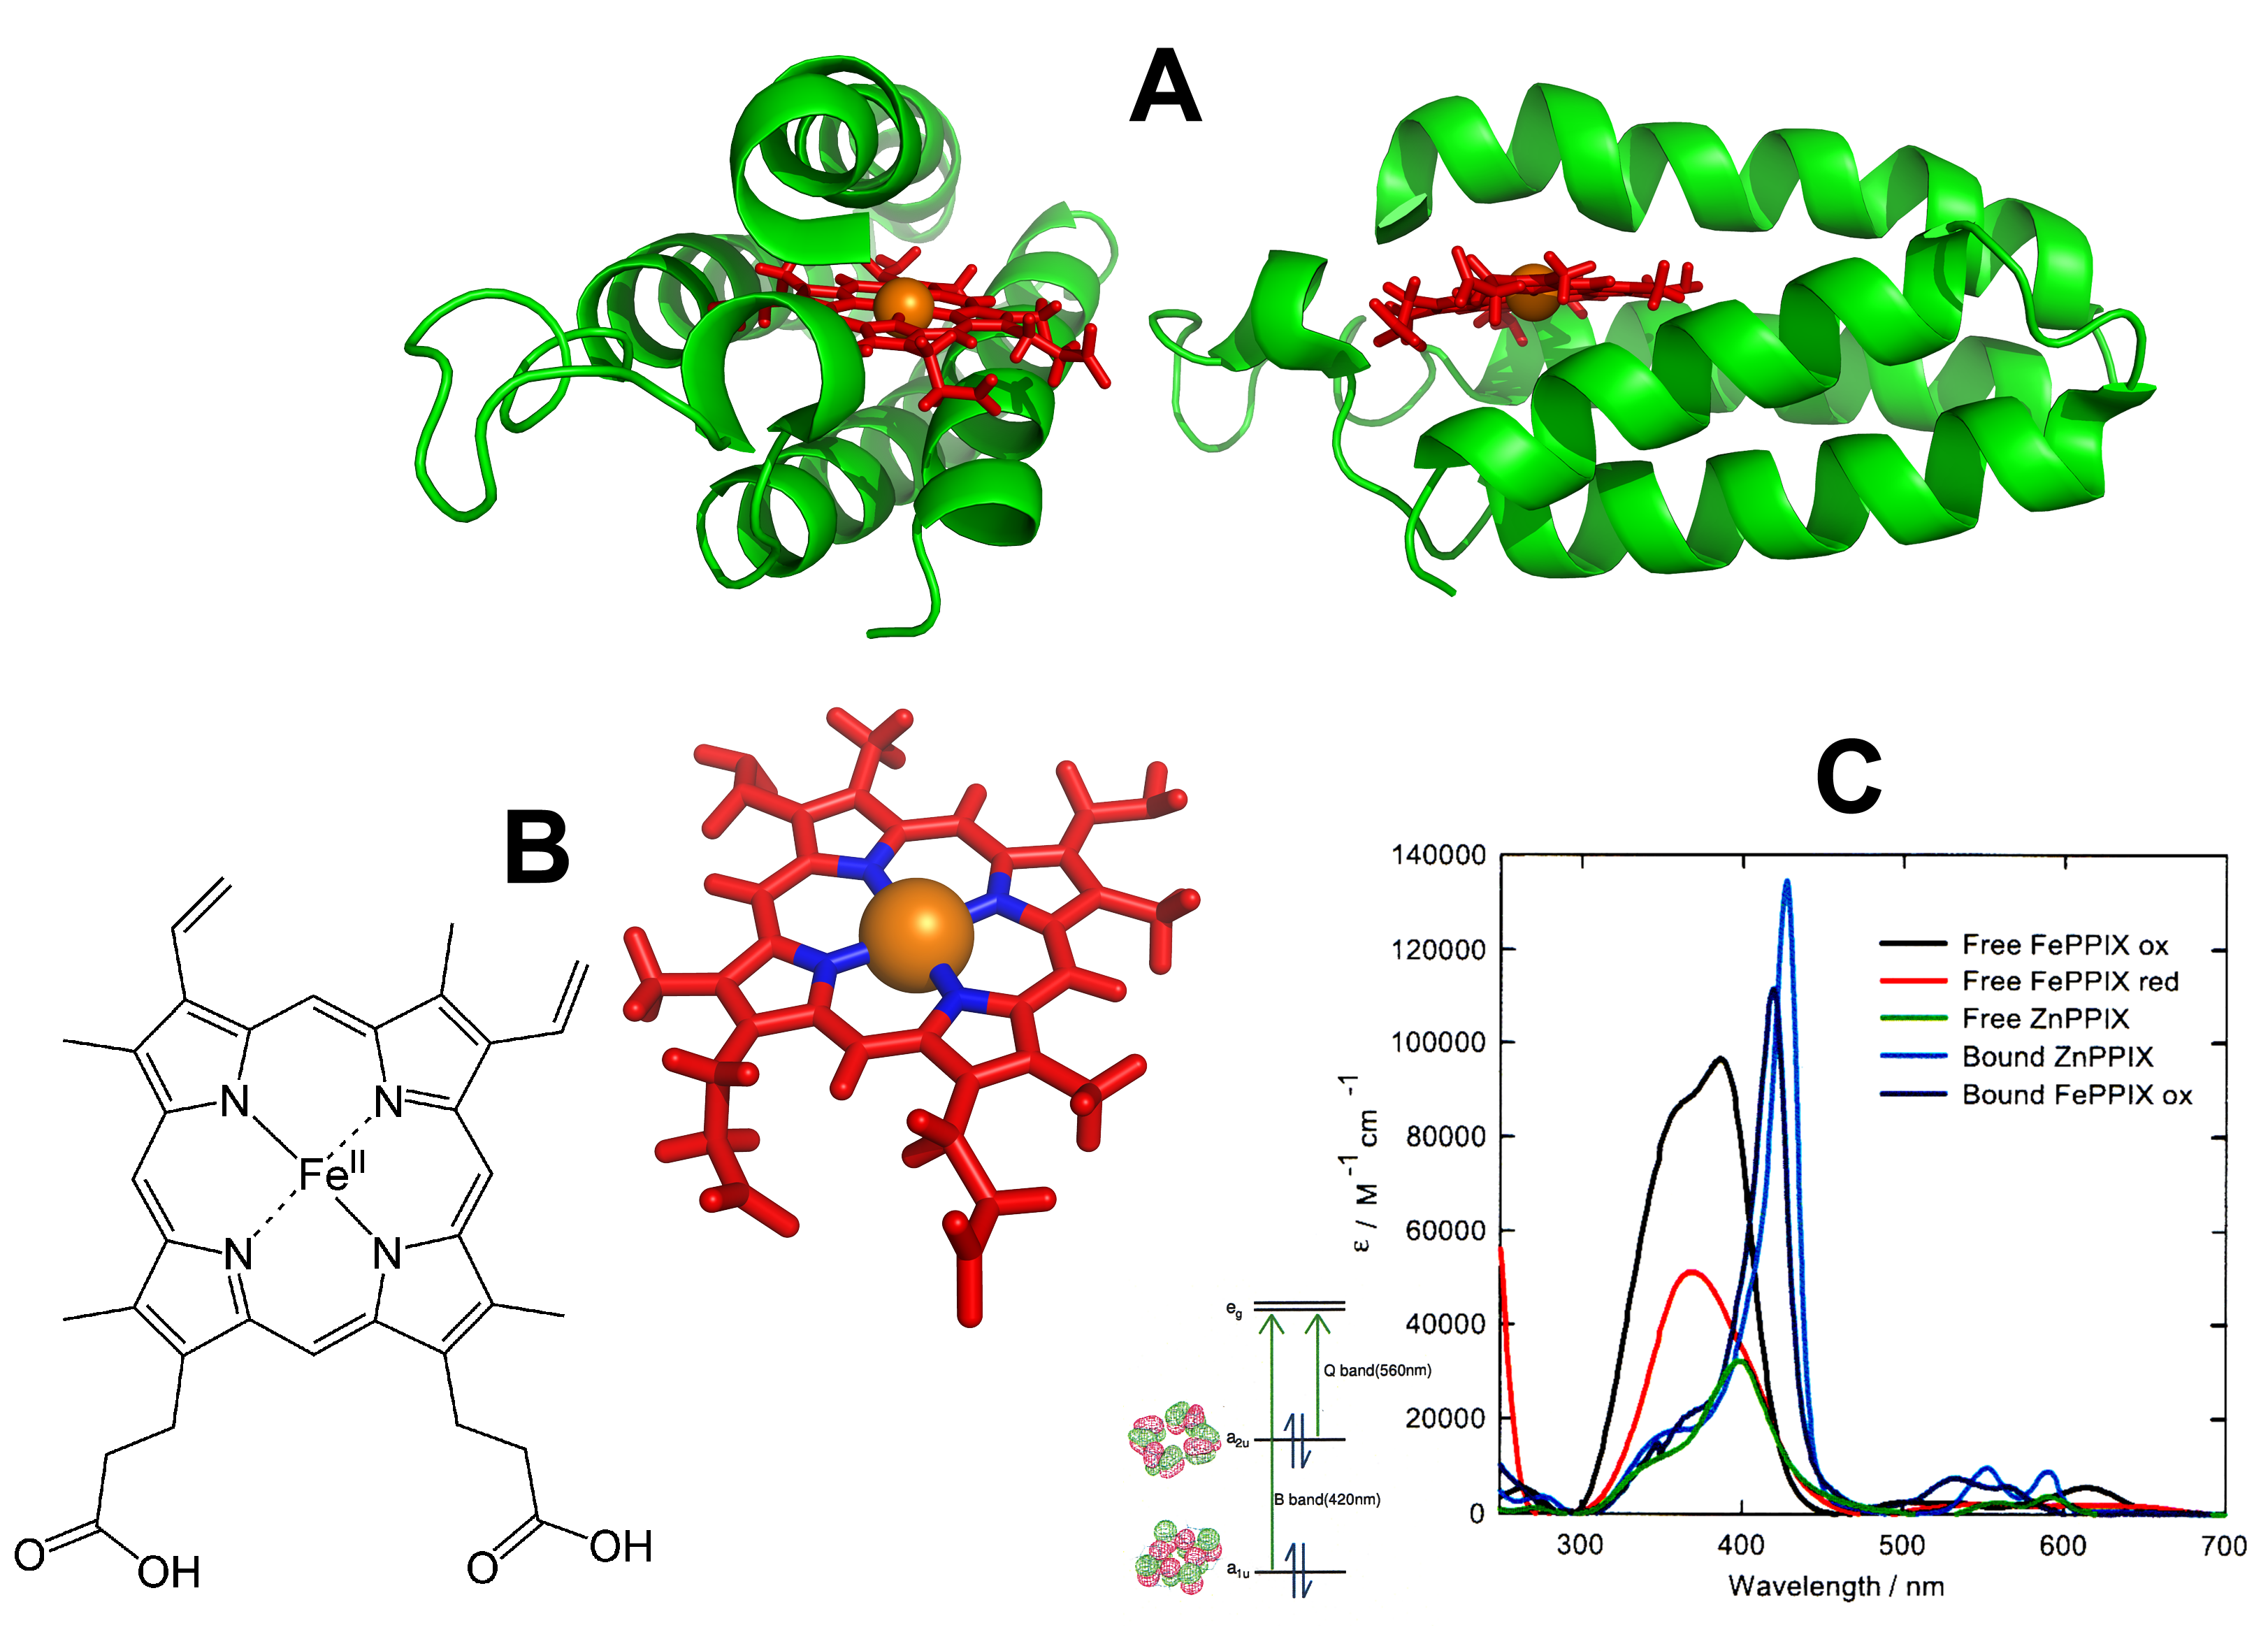
\includegraphics[width=137.4mm]{Images/haemStructure.png}
	\caption[Haem Structure]{A fancy image.}
	\label{fig:haemStructure}
\end{figure}
\end{verbatim}

\vspace{2ex}

\begin{figure}[!th]
	\centering
	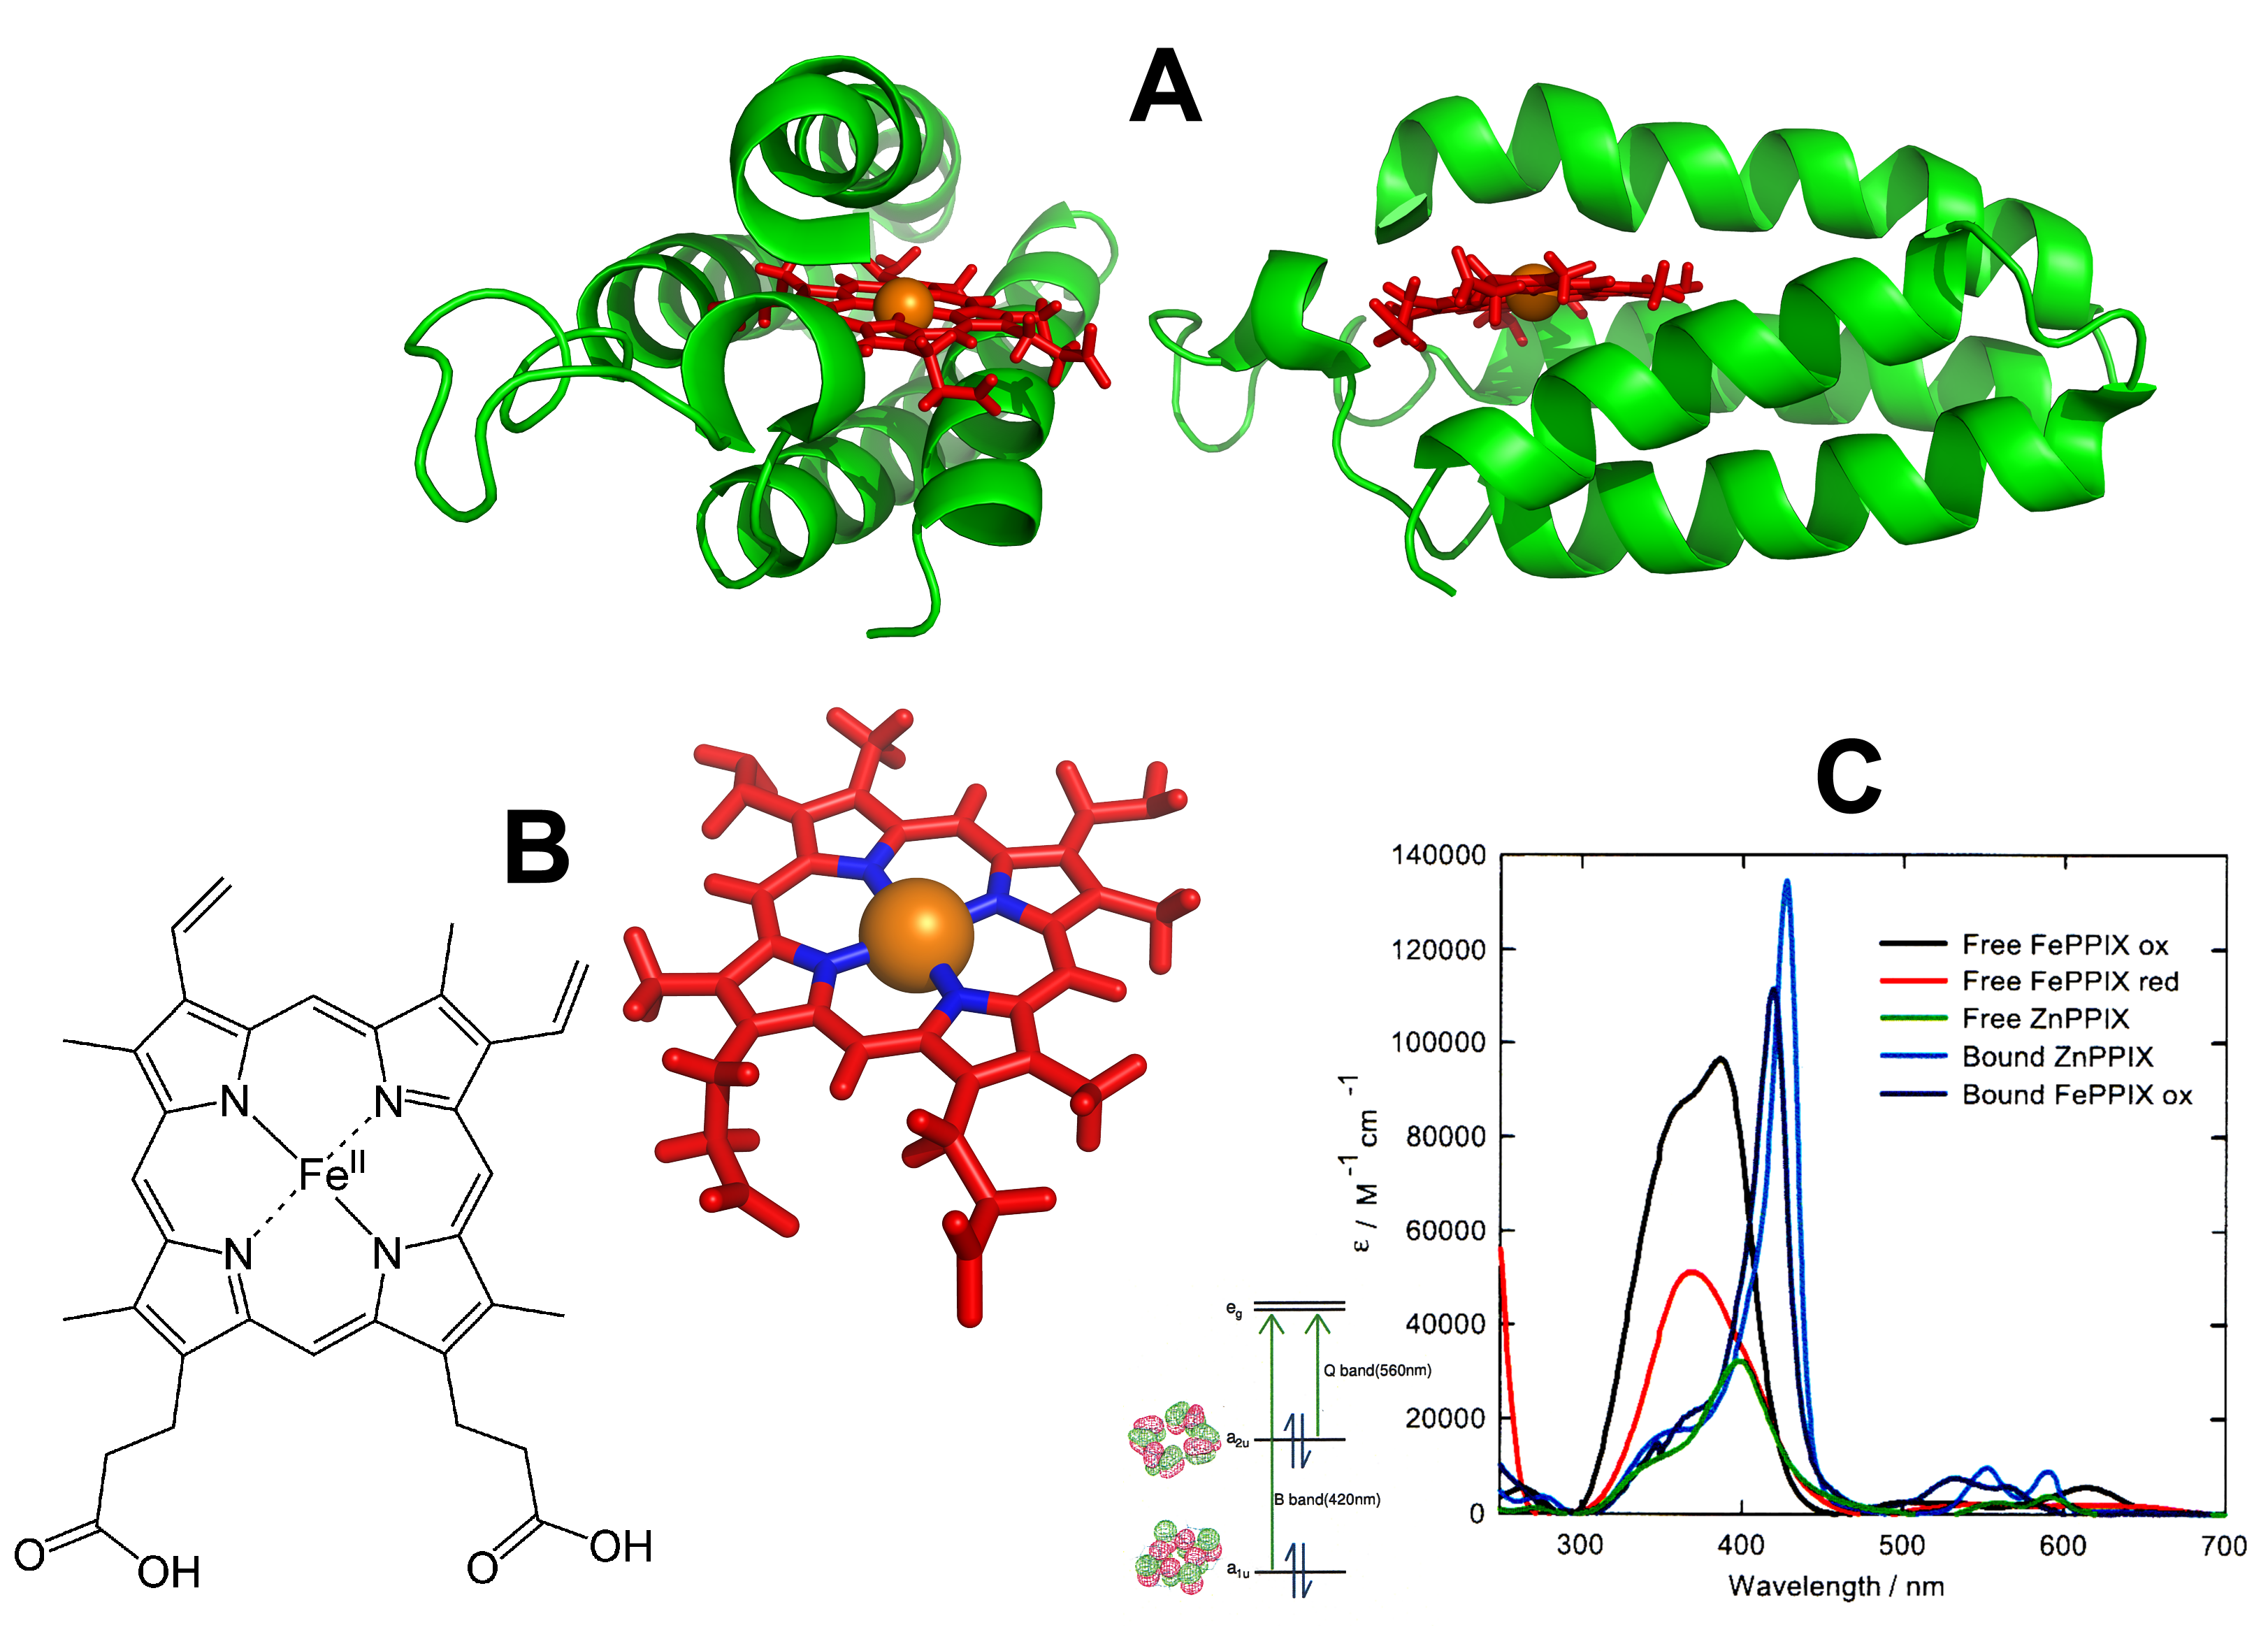
\includegraphics[width=137.4mm]{Images/haemStructure.png}
	\caption[Haem Structure]{A fancy image from Chris' Thesis.}
	\label{fig:haemStructure}
\end{figure}

In this example the command {\textbackslash}includegraphics tells LaTeX to look in the directory `Images' and incorporate the file called `haemStructure.png' into the final document while setting the width to 137.4mm.  This command can be used to resize a graphical file using the height or width parameter as shown. You must specify the units which can be pt, ex, em, mm, cm and so on. LaTeX recognises a very wide variety of standard units and graphics formats. The command is part of the graphicx package and so in the preamble you must include the command {\textbackslash}usepackage\{graphicx\}.

Many packages have been written to provide new commands. For example the `subfigure' package enables you to place separate images or files in the same figure side by side while giving them their own label. However, in this document we only concentrate on the very basics.

\section{Floating Environments}

Both tables and figures are examples of a `floating environments' which means LaTeX decides where to put them. 

The mysterious [!tbh] letters give guidance to LaTeX about roughly where the figure or table is  allowed to be, but in general they can move a long way from where you position them within your text file.  The letters in the square bracket can be t, h or b which stand for top, here or bottom.  If you don't specify any letters LaTeX defaults to [t].

LaTeX will always preserve the order in which figures appear.  If it cannot find a type setting solution, then it may move the float to it's own page, and combine it with other figures. If it still can't fit that in for some reason then it moves the float to the end of the document.  This has the effect of pushing all the remaining floating environments to the end of the document also.

The exclamation mark instructs LaTeX to ``try harder'' at putting the float where you told it to. Often you must play around to ensure the float positioning is acceptable, but usually this can be achieved by stretching or shrinking the image slightly using the size parameter, re-ordering text, judicial applications of the {\textbackslash}pagebreak command or by shouting loudly and slapping the computer monitor about. Note that it is better to resize the image using the original program that was used to create the image. Also using vector graphics can assist be useful (e.g. eps files) because they are designed to scale better.
\chapter{The Chapter on Making Chapters}
\label{sec:Chapters}

Right. LaTeX forces you to structure your document. There a series of simple commands for achieving this:

\vspace*{2ex}

{\textbackslash}chapter\{chapterName\}

{\textbackslash}section\{sectionName\}

{\textbackslash}subsection\{subsectionName\}

{\textbackslash}subsubsection\{subsubsectionName\}

\vspace*{2ex}

Easy enough. At the start of each chapter or section just issue one of these commands to name the section and LaTeX will present the chapter heading in the right style of font, which will be the same style of all the other heading names at that level of hierarchy throughout the document. In addition LaTeX assigns a number to that section. For example, this chapter was created using the command:

\vspace*{2ex}

{\textbackslash}chapter\{The Chapter on Making Chapters\} 

\vspace*{2ex}

LaTeX assigns the correct chapter number to each chapter in turn and then puts it in the table of contents, as you can see by looking at the table of contents! Easy.

\pagebreak
\section{The Section About Sections}
\label{sec:Section}
I think you're getting the hang of this. This section was created using the command {\textbackslash}section\{The Section About Sections\}. It appears in the table of contents as section \ref{sec:Section}.

\subsection{The Sub-Section About Sub-Sections}
\label{sec:SubSection}
Now you're really getting the hang of this. This subsection was created using the command {\textbackslash}subsection\{The Sub-Section About Sub-Sections\}. 

\subsubsection{The Sub-Sub-Section About Sub-Sub-Sections}
\label{sec:SubSubSection}
Now you're really getting the hang of this. but.. caught you out! This subsubsection doesn't have a number!  Ha Ha! It was created using the command {\textbackslash}subsubsection\{The Sub-Sub-Section About Sub-Sub-Sections\} in the same vein as all the other subsections/chapters etc. Here we have stopped the depth of the section numbering at the second level with the command:

\vspace*{2ex}

{\textbackslash}setcounter\{secnumdepth\}\{2\}

\vspace*{2ex}

Easy. WYSIWYM.  LaTeX does what you tell it to do. This is both a blessing and a curse.

\pagebreak
\section*{The Section About Sections That Don't Appear in the Table of Contents}
\label{sec:InvisibleSection}
Ok. Now we're throwing a spanner in the works. This section was created using the command:

\vspace*{2ex}

{\textbackslash}section*\{The Section About Sections That Don't Appear in the Table of Contents\}. 

\vspace*{2ex}

Notice how LaTeX has not assigned a number to the section and it doesn't appear in the table of contents. The effect of the * is to suppress the inclusion of a chapter, section or subsection in the automatic numbering. Easy. You can do this at any level. This is useful for things like prefaces, tables of contents or acknowledgements which you may or may not wish to have an entry in the main contents table. Up to you. It's your thesis. Don't just copy me.

\section{A Small Point About Numbering}

In this section notice how the numbering starts from where it left off before we suppressed the numbering on the previous section. Easy. WYSIWYM.
\pagebreak
\section{The Section About Internal Referencing}
\label{sec:InternalReferencing}

There are two related commands:

\vspace*{2ex}

{\textbackslash}label\{labelName\} 

{\textbackslash}ref\{labelName\}

\vspace*{2ex}


The {\textbackslash}label\{\} command allows you to create a label in a particular environment\footnote{That's right. Chapters, Sections and sub-sections etc are environments!}. The label won't appear in the final document. It's just a label which makes it easy to refer back to any particular environment elsewhere in the document. The {\textbackslash}ref\{\} command enables you to insert a reference anywhere in the document to any label in the document.  For example this is section \ref{sec:InternalReferencing}. The names you use in a label can be anything you like but musn't contain whitespace or special characters. I used the two commands:

\vspace*{2ex}

{\textbackslash}label\{sec:InternalReferencing\}

{\textbackslash}ref\{sec:InternalReferencing\}.

\vspace*{2ex}

The astute among you will realise that LaTeX has to read the document several times. Once to find the labels and then again to populate the references with the correct numbers. So you have to compile a latex document twice to get the referencing right. If there is a missing label or you refer to something that doesn't exist then latex inserts a convenient ? at that point. So hunting for queries is useful way of finding broken references. Latex issues warnings when it finds broken references.

As you create a document you will find yourself putting labels in all over the place so choose a sensible naming convention to help you remember the label names.

Each type of environment (equations, figures, tables, sections etc) has its own independent numbering system.  So when you choose your label name it's a good idea to have an identifier for that type of environment.  I have my own convention for label names which I use to help me remember references. E.g.   sec:SectionAboutCats. Eqn:EquationAboutCats,  Fig:FigureAboutCats and so on. This means you can differentiate between referring to the section or the figure more easily, even though they are about the same thing.

So Internal Referencing is a doddle. Easy!
\chapter{External Referencing}

Referencing is usually performed using a separate program called BibTex.  This program understands the file format .bib.

To create a reference within your document first you must create a .bib file by exporting your list of references from which ever referencing software you used, such as endnote, mendeley or whatever you use.

You can refer to an entry in the .bib file using the {\textbackslash}cite\{ref:Name\} command. the identifier `ref:Name' is the unique identifier which is the first line of each item included in your bibliography file.

For example, open the file LaTexCourseBib.bib in the bibliography directory. The first entry has the identifier `Horcas2007'.  This can be invoked as follows:


\begin{verbatim}
For example, this interesting fact\cite{Horcas2007}, is a cracking example.
\end{verbatim}

For example, this interesting fact\cite{Horcas2007}, is a cracking example.

During compilation latex and bibtex co-operate. During the first compilation latex generates a list of references that it needs.  During the second compilation bibtex populates the details from the .bib file into a shorter, ordered .bib file. The third compilation inserts markers at the right place in the main file and the fourth compilation generates the final list of references. Thus the compilation sequence is latex, bibtex, latex, latex.

The style of the referencing format can be changed using the command {\textbackslash}bibliographyStyle\{\}. e.g. the style used in this document is cjfthesisv1.bst which is invoked by 

\begin{verbatim}
\bibliographystyle{Bibliography/cjfthesisv1}
\end{verbatim}

The location of the list of references in the document is specified by issuing the {\textbackslash}bibliography\{\} command which also specifies the master bibliography file.

\begin{verbatim}
\bibliography{Bibliography/LaTeXCourseBib}
\end{verbatim}




\chapter{Organising Your Files}
One of the drawbacks of word is that the figures and tables are included within the document which becomes very very clunky quite quickly and once it reaches around 100Mb it becomes unwieldy and hard to export. One of that advantages of LaTeX is that the files are all text files and so are very light on resources and are easy to email around the place.

However, sometimes it can be difficult to navigate through a single text file, so if you had a huge document then it becomes difficult to find your way around.  One way of circumnavigating this problem is to break the file up into smaller files. As long as LaTeX knows where to look you can have a file for each logical sub-division of your document.

Therefore it is worth spending a bit of time at the beginning of a large project deciding how you wish to break up your LaTex Files and organise them neatly and tidily.  You can then tell LaTex where to look for the files using the following command:

\vspace*{2ex}
{\textbackslash}include\{fileName\}
\vspace*{2ex}

\pagebreak
\section{Linking a File}
We are now going to copy part of the tutorial file into a separate files and link it the main file.  Because this could go wrong it is sensible to back up tutorial.tex as something else. So save a copy called `tutorialOriginal.tex' for safe keeping. Then follow the following instructions.

\begin{enumerate}
\item Create a new file called MyFirstPage.tex
\item Select and Cut out the first chapter of Tutorial.Tex
\item Paste the first chapter into MyFirstPage.tex
\item Save both tutorial.tex and MyFirstPage.tex
\item Then add {\textbackslash}include\{MyFirstPage\} in tutorial.tex where the text used to be before you cut it out. We don't need to add the `.tex' because LaTeX can only include `.tex' files.
\item compile tutorial.tex and view the PDF
\end{enumerate}

The final PDF should look exactly the same as it was! except we now have a separate file for one of the chapters.

\pagebreak
\section{Creating A Class File}
We can also save our preamble in a separate file called a class file. This makes your main document much easier to understand.  To make it work we need to use the {\textbackslash}LoadClass\{\} command as follows: 

\begin{enumerate}
\item Create another new file and save it as TutorialStyle.cls
\item Copy the preamble of tutorial.tex into the new file. Starting with the {\textbackslash}documentclass{} command and copy right up to, but not including, the {\textbackslash}begin{document} command. Delete the preamble in the original document.
\item Save TutorialStyle.cls and tutorial.tex
\item Modify the first line of TutorialStyle.cls by replacing the word `document' with the word `Load'.
\item Add a new first line of tutorial.tex to use your new style class {\textbackslash}documentclass\{TutorialStyle\}
\item Save both files.
\end{enumerate}

\subsection{Sanity Check}

The first line of TutorialStyle.cls should now be:

\begin{verbatim}
\LoadClass[12pt, oneside, a4paper]{book}
\end{verbatim}
\vspace{2ex}

The first line of tutorial.tex should be:

\begin{verbatim}
\documentClass{TutorialStyle}
\end{verbatim}
\vspace{2ex}

We have just created what is called a style file. You can use this style file as a generic preamble for other documents as well. Compile tutorial.tex.  Nothing should have changed in the final PDF.


\pagebreak
\section{The Structure of this Document}

Lets now look at how I've organised this document. It is identical to my thesis because it started out life as my thesis. I usurped the structure and simply replaced the headings and content to make a kind of reference manual for this introductory course. This document therefore is three things:

\begin{enumerate}
\item An example thesis structure to work from.
\item The LaTeX files which were used to create it can be used as a template for a thesis.
\item It is also a convenient introductory latex manual!
\end{enumerate}

\vspace*{2ex}
Groovy huh?

\section{The Master File}

There is a master file where LaTeX begins the compilation procedure. This contains the {\textbackslash}documentclass command needed to set the ball rolling. Within the file there are a series of {\textbackslash}include\{\} commands, one for each Chapter, which tell LaTeX where to find the files containing each chapter.

The subfiles cannot be compiled on their own because they do not contain the {\textbackslash}documentclass, {\textbackslash}begin\{document\} or {\textbackslash}end\{document\} commands. Lets us look in more detail at the master file and we will learn some new LaTeX commands.

\singlespacing
\pagebreak
\begin{verbatim}
\documentclass{Style/LatexCourseStyle}

\begin{document}
\setcounter{secnumdepth}{2}
\setcounter{tocdepth}{1}

\frontmatter
\onehalfspacing
\thispagestyle{empty}

\begin{center}
\vspace*{\stretch{1}}

\hrule height 2pt
\vspace*{2ex}
{\Huge\textbf{Towards the Ability to Make Super Duper LaTeX Documents}\par}
\vspace*{2ex}
\hrule height 2pt
\vspace*{10ex}
{
\includegraphics[height=40mm]{Images/UnivShield}\par}
\vspace*{10ex}
{\large\textbf{Christopher~James~Forman}\par}
\vspace*{2ex}
{\large{Department Of Chemistry}\par}
\vspace*{2ex}
{\large{University of Cambridge}\par}
\vspace*{5ex}
{\large{This dissertation is submitted for the degree of \textit{Doctor of Philosophy}}\par}
\vspace*{5ex}
{\large{\today}\par}

\vspace*{\stretch{2}}
\end{center}
\chapter*{Declaration}

\vfill

This dissertation is the result of my own work and includes nothing which is the outcome of work done in collaboration except where specifically indicated in the text. It is not substantially the same as any that I have submitted for a degree or diploma or other qualification at any other University and no part has already been, or is concurrently being, submitted for any degree, diploma, or other qualification. It does not exceed 60,000 words, including tables, footnotes, bibliography and appendices.\par

\vspace{10ex}

\begin{flushright}
Signature: \rule[0pt]{60mm}{0.5pt}

\vspace{5ex}

Date: \rule[0pt]{60mm}{0.5pt}
\end{flushright}

\vfill
\chapter*{Acknowledgments}
\subsection*{Family}
Mum. Dad. Pet Dog.

\subsection*{Scientific Collaborations}
Dr A.N.Other at uni of blah for samples and instrument time etc. My Amazing Lab Chums.

\subsection*{Scientific Support}
My amazing lab chums.

\subsection*{General Assistance}
Cleaner, My amazing lab chums.

\subsection*{Financial Support}
Bank, Tax payer. My amazing lab chums.

\subsection*{Moral Support}
My Amazing Lab chums.

\subsection*{Academic Inspiration}
Netwon, My super. My Amazing Lab Chums.

\subsection*{Everyone else}
My Amazing Lab Chums.

\chapter*{Summary}
This document is a handbook for introducing you to LaTeX. It contains a bit of background about the history and philosophy of LaTeX.  However, it concentrates on providing a guided practical introduction to the basic techniques such as 
\begin{itemize}
\item Lists
\item Mathematical and chemical equations
\item Tables
\item Figures
\item Chapters and Sections
\item Linking to other files in large documents
\item Referencing
\end{itemize}

The handbook is also presented in the style of a thesis. This means that source files provided on the introductory course and available from the department web page are a convenient template for a thesis.

More details on specific aspects of LaTeX can be found at the departmental LaTeX page which can be found here:

 http://www-ch-int.ch.private.cam.ac.uk/latex/about

\chapter*{Abbreviations}

\begin{longtable}{r >{\rule{0pt}{3ex}}l<{\rule[-1.5ex]{0pt}{0pt}}}
ADP & Adenosine Diphosphate\\
(nc/c)AFM & (non-contact/conducting) Atomic Force Microscopy\\
ATP & Adenosine Triphosphate \\
\end{longtable}
\tableofcontents
\listoftables
\listoffigures

\mainmatter
\renewcommand{\sectionmark}[1]{\markright{\thesection \ #1}{}}
\chapter{Overview}
\label{chap:overview}
\section{LaTeX: The answer to everything.}
LaTeX is typsetting program that takes an input file of marked up text and then, with a user defined set of rules, typesets a beautifully crafted output file that can be easily printed (e.g. a pdf). 

\subsection{Advantages}

The advantages of this method are manifold:

\begin{itemize}

\item Use any text editor to view the source document.
\item More time can be spent working on the content and not worrying about how text or figures interact in the layout until later on.
\item LaTeX uses consistent rules throughout a document
\item LaTeX sorts out basic typesetting automatically
\item Changes can be introduced globally with very little effort
\item Document structure is explicit
\item Documents can be professionally typeset and look great
\item You are forced to structure your documents correctly.
\item Mathematical equations, like $E=mc^2$ or $\imath\hbar\frac{\partial}{\partial t}\Phi (x, t) = \hat{H}\Phi (x, t)$ can be produced almost as fast as typing (if you know the commands!).
\end{itemize}

\subsection{Disadvantages}
The disadvanatges of this method are also manifold:
\begin{itemize}
\item You don't see the output as you go.
\item Steep learning curve.
\item Documents are harder to edit by a second author (unless they are adept at LaTeX too). This can be mitigated using version control, which makes group authoring processes superior to word.
\item The program never works quite the way you want it to and learning how to influence it can be problematic and subtle.
\item Although intended to save work the principle of 'conservation of work' means that you simply transform problems associated with WYSISYG approaches to problems associated with WYSIWYM approaches!
\item You can go blind trying to determine the difference between wiggly and smooth brackets if your editors font isn't large enough.
\end{itemize}

\subsection{On balance?}
If it's so rubbish, why use LaTeX?

\begin{itemize}
\item Large documents are much more easily handled. 
\item In general it is quicker to debug a LaTeX document than typeset an entire thesis manually. 
\item Technical information such as tables, equations and figures are integrated much more smoothly than with word.
\end{itemize}

\section{How does it work?}

The raw text is interspersed with commands, preceded by a \textbackslash, which tell LaTeX what to do with the text. For example you can \textbf{make it bold}, \emph{italic}, or \underline{underlined} with the commands {\textbackslash}textbf\{\}, {\textbackslash}emph\{\} or {\textbackslash}underlined\{\}. More on commands in a moment...



\chapter{My First Page}

\section{The Very Beginning}
The very simplest LaTeX document might look like this:

\begin{verbatim}
\documentclass[a4paper,12pt]{article}
\begin{document}
Hello World.
\end{document}
\end{verbatim}

\pagebreak
\thispagestyle{empty}
Hello World.
\pagebreak
\subsection{Break Down}
What's all the gobbledegook around my simple message???

In LaTeX we intersperse text and commands.  Commands are preceded by a \textbackslash. For example the first line in a LaTeX document \underline{\textbf{\emph{must}}} be:

\begin{verbatim}
\documentclass[options]{class}
\end{verbatim}

Where the word ''class'' may be substituted for one of many things such as: article, proc, minimal, report, book, letter, memoir, slides, beamer.

Similarly, and completely generally in LaTeX speak, the square brackets denote the existence of optional parameters. Each individual command can take its own parameters and for the ''{\textbackslash}documentclass'' command there are options for controlling font size, font family, landscape, oneside, twosided, page size and so on. These options will persist throughout the entire document. For example the document class command for this document, (which is likely to be like the one you would use for a thesis), would be:

\begin{verbatim}
\documentclass[12pt, oneside, a4paper]{book}
\end{verbatim}

Other options include:

\begin{itemize}
\item {10pt, 11pt, 12pt (default is 10pt).}
\item {letterpaper, legalpaper, a4paper, executivepaper, a5paper, b5paper}
\end{itemize}
and so on.

\pagebreak
\section{Can I start typing please?}

After we have set up the document we can start actual work on our document. So we must tell LaTeX that what follows is to be interpreted as a document.  The command {\textbackslash}begin can take many different parameters and is a command to enter what is known, in LaTeX speak, as 'an environment'. Thus the commands:
\begin{verbatim}
\begin{document}

\end{document}
\end{verbatim}

tells LaTeX to enter and leave the document environment, and thus constitute the outer limits of our document file. Other environments include the equation environment, the itemize environment, the figure environment and so on. These will be encountered in due course.

Every part of the LaTeX file is therefore within an environment of specific type and the content within each environment consists of commands or text.

That's basically it.

So let's get on with it shall we...

\pagebreak
\section{The ground rules}
\begin{quote}
Hold on, hold on, hold on my son.

First the lessons.

Then the fun!
\end{quote}
Dr Seuss.

\subsection{Spaces}
Whitespace characters, such as blank or tab, are treated uniformly as space by LaTeX. Several consecutive whitespace characters are treated as one single space. Whitespace at the start of a line is generally ignored, and a single line break is treated as whitespace. An empty line between two lines of text defines the end of a paragraph. Several empty lines are treated the same as one empty line. The text below is an example.

\begin{verbatim}
It does not matter whether you
enter one or several             spaces
after a word. The final result will be typeset beautifully
according    to     precise rules.




An empty line starts a new
paragraph. Note the indentation on the first line of the paragraph, 
except at the beginning of the section. 
\end{verbatim}

\vspace*{2ex}
\vspace*{2ex}

It does not matter whether you
enter one or several             spaces
after a word. The final result will be typeset beautifully
according    to     specific rules.




An empty line starts a new
paragraph. Note the indentation on the first line of the paragraph, except at the beginning of the section. 

\pagebreak
\subsection{Special Characters}
The symbols 

\# \$ \% \textasciicircum{} \& \_ \{ \} \~{} \textbackslash

are reserved characters that either have a special meaning under LaTeX or are unavailable in all the fonts. If you enter them directly in your text, they will normally not print, but rather make LaTeX do strange things.

To overide the special meanings of these symbols and allow them to produced within your text you may use the following sequences:
\begin{verbatim}
\# \$ \% \textasciicircum{} \& \_ \{ \} \~{} \textbackslash
\end{verbatim}

Other symbols and many more can be printed with special commands in mathematical formulae or as accents.

The backslash character '\textbackslash' cannot be entered by adding another backslash in front of it ( \textbackslash\textbackslash); because this sequence means ''linebreak''.

The command \textbackslash\~{}\{\} produces a tilde which is placed over the next letter. For example \textbackslash\~{}\{n\} gives \~{n}. To produce just the character \~{}, use \textbackslash\~{}\{\} which places a \~{} over an empty box.

Similarly, the command \textbackslash\textasciicircum{} produces a hat over the next character, for example \textbackslash\textasciicircum\{o\} produces \^{o}.

\pagebreak
\section{Preamble}
After the {\textbackslash}documentclass command we add ''preamble''. Here we load special features that we will use throughout our document to expand on the basic capabilities of LaTex. These are contained in units called ''packages'' which we can tell our LaTeX compiler to download by using the command ''{\textbackslash}include\{packageName\}''. 

There are many repositories of such packages on the web. Your compiler generally knows where to look and most standard packages are included with any install. For example, to include a special set of typesetting instructions to handle chemical equations we can grow our simple document with a single command like this:

\begin{verbatim}
\documentclass[a4paper,12pt]{article}
\usepackage[version=3]{mhchem}
\begin{document}
Hello World!

We all need \ce{H2O}.

I'm less fussed about \ce{^{235}_{92}U+}.

\end{document}
\end{verbatim}

\vspace{2ex}

\pagebreak
\thispagestyle{empty}
Hello World!

We all need \ce{H2O}.

I'm less fussed about \ce{^{235}_{92}U+}.
\pagebreak

Here we have loaded a package called: "`mhchem"' which took the option ''[version=3]''. This is a package for drawing chemical equations easily and it has it's own instruction manual which you can follow easily. It is included in the bundle of files for this course.

Other things we can do in the premable within LaTeX are to redefine existing commands or create our own personal commands. These can be stored in a file called the 'style file' which we can load at the beginning of our document, in place of our documentclass. More about this later on...


\subsection{Comments}
It is often useful to comment your LaTeX documents. You can leave yourself amusing, sarcastic messages that won't get printed out in the final document. Use this to make your own notes as the course progresses.

To get a comment use the \% command, which tells LaTeX to ignore the rest of the line, the line break and all the white space at the beginning of the next line, for example, we may add to our continually evolving document...

\begin{verbatim}
\documentclass[a4paper,12pt]{article}
\usepackage[version=3]{mhchem}
\begin{document}
Hello World!

%All humans need water and I would like 
%to include this concept in my arguments.
We all need \ce{H2O}.

%Uranium 235 is toxic, which is why I don't want to consume it... 
I'm less fussed about \ce{^{235}_{92}U+}.

\end{document}
\end{verbatim}

\vspace{4ex}
Hello World!

%All humans need water and I would like to include this concept in my arguments.
We all need \ce{H2O}.

%Uranium 235 is toxic, which is why I don't want to consume it... 
I'm less fussed about \ce{^{235}_{92}U+}.

\pagebreak
\section{Compiling}
Once the document is finished you can compile it. Your compiler will depend on the platform that you use. In the PWF we are using winEDT to edit the documents (a LaTeX front end) and texlive2008 which is the compiler itself. I use MiKTex and the front end texCenter.  There is no need to use a front end. If you prefer you can use a simple text editor and a command line.

the recommended distributions are:
\begin{itemize}
\item MiKTeX or TeX Live for Windows
\item TeX Live for Unix/Linux
\item MacTeX or TeX Live for Mac OS.
\end{itemize}

Once you have installed your software and got it working, written your source code and tried to compile it, there will nearly always be something wrong with your file. 

Any errors will be highlighted in the console window or error output box of your front end.  Some front ends dump the running commentary which LaTeX produces into a text file for easy reading afterwards.

In a compile attempt (successful or otherwise) LaTeX may produce the following files:

projectname.aux

projectname.bbl

projectname.lof

projectname.lot

projectname.txt

projectname.toc

projectname.dvi

These are interim files (toc= table of contents, bbl = bibliography etc). To be honest I have no idea what half of these things contain.  You only need the .tex file and a compiler with the right packages installed to produce them again.

Some versions of LaTeX only produce DVI files and you then need to convert the dvi file to a PDF or download a dvi viewer. You can also convert DVI files to PS files and then view them.  The good thing about front ends is that you can set them up to produce PDFs directly.

OK. So we have now produced a silly document but we understand it.  Now lets get on with learning how to make our own documents.



\chapter{Lists}
Lists are great.  The command {\textbackslash}begin\{\} can be used to enter a list environment.  For example:

\begin{verbatim}
\begin{itemize}
\item cat
\item dog
\item horse
\end{itemize}
\end{verbatim}

Produces:

\begin{itemize}
\item cat
\item dog
\item horse
\end{itemize}

\pagebreak
We can also replace the bullet points with numbers using the enumerate keyword.

\begin{verbatim}
\begin{enumerate}
\item cat
\item dog
\item horse
\end{enumerate}
\end{verbatim}

\begin{enumerate}
\item cat
\item dog
\item horse
\end{enumerate}

\pagebreak
and we can use the description keyword which does this:
\begin{verbatim}
\begin{description}
\item[Cat] a lovely furry creature with a cute nose and whiskers.
\item[Dog] Another furry creature that smells rather well; 
           its olfactory power stems from its nasal dampness.
\item [Horse] A large stinky creature with sideways facing eyes.
\end{description}
\end{verbatim}

\begin{description}
\item[Cat] a lovely furry creature with a cute nose and whiskers.
\item[Dog] Another furry creature that smells rather well; its olfactory power stems from its nasal dampness.
\item [Horse] A large stinky creature with sideways facing eyes.
\end{description}
\chapter{Maths Equations}

\section{Producing Beautiful Looking Mathematics}

One of the best features about LaTeX is `maths mode'.  For example the schrodinger equation can be produced as follows:

\vspace*{2ex}

\begin{center}
\begin{math}
\imath\hbar\frac{\partial}{\partial t}\Phi (x, t) = \hat{H}\Phi (x, t)
\end{math}
\end{center}

\vspace*{2ex}

\begin{verbatim}
\begin{math}
\imath\hbar\frac{\partial}{\partial t}\Phi(x,t)=\hat{H}\Phi(x,t)
\end{math}
\end{verbatim}

There are a number of ways to switch on maths mode.  The first, as above, is with the {\textbackslash}begin\{math\} environment. You can also enter mathmode inline using the \$ symbol. For example typing in \$y=ax\textasciicircum{}2+bx+c\$ yields $y=ax^2+bx+c$.  Another way is to enter the equation environment which enables you to number equations so you can then refer to them later in the text.

\begin{equation}
y(t)= \sin \left(\frac{{\alpha}t}{2\pi} + \phi_0\right)
\label{eqn:MadeUpNonsense}
\end{equation}

\vspace*{2ex}
\begin{verbatim}
\begin{equation}
y(t)= \sin \left(\frac{{\alpha}t}{2\pi} + \phi_0\right)
\end{equation}
\end{verbatim}.

\section{Basic Maths Mode}
Once in maths mode there is a kind of text based code for writing down your equations.  Here are the most basic symbols to get you going.
\begin{center}
\begin{tabular}{cc}
\toprule
Final Result & LaTeX Code \\
\cmidrule(){1-2}
$a+b$ & a+b \\
$a-b$ & a-b \\
$ab$ & ab \\
$a*b$ & a*b \\
$a \times b$ & a {\textbackslash}times b \\
$a \cdot b$ & a {\textbackslash}cdot b \\
$\frac{a}{b}$ & {\textbackslash}frac\{a\}\{b\} \\ 
$a^b$ & a\textasciicircum{}b \\
$a_b$ & a\_b \\
$\sin a$ & {\textbackslash}sin a  (same for cos, tan)\\
$ sin a$ & sin a \\
$\sqrt{a}$ & {\textbackslash}sqrt\{a\} \\
$\left( a \right) $ & {\textbackslash}left( a {\textbackslash}right)\\ 
$\left[ a \right]$ & {\textbackslash}left[ a {\textbackslash}right]\\ 
$\alpha$ & {\textbackslash}alpha \\
$\pi$ & {\textbackslash}pi \\
\bottomrule
\end{tabular}
\end{center}

A full treatise on maths mode is not practical here. There are lots of online tutorials and summaries of symbols. It just takes a bit of practice and you can build up equations really easily. It's straight forward to learn new stuff once you've done it a few times.

\pagebreak
\section{Equation Arrays}
Sometimes you need to arrange several equations vertically, referencing individual lines separately and aligning the equations on the $=$ sign. This can be achieved with equation arrays as follows:

\begin{eqnarray}
A\left( x\right) & = & \frac{x^2+2x+1}{x+1} \\
& = & \frac{\left(x+1\right)\left(x+1\right)}{x+1} \nonumber\\
& = & x+1 \nonumber\\
B(x,t) & = & \frac{e^{\left(\imath\omega_0 t + kx\right)}}{4\pi\epsilon_0}
\end{eqnarray}

\begin{verbatim}
\begin{eqnarray}
A\left( x\right) & = & \frac{x^2+2x+1}{1+x} \\
& = & \frac{\left(x+1\right)\left(x+1\right)}{1+x} \nonumber\\
& = & x+1 \nonumber\\
B(x,t) & = & \frac{e^{\left(\imath\omega_0 t + kx\right)}}{4\pi\epsilon_0}
\end{eqnarray}
\end{verbatim}

\begin{itemize}
\item Note the \& symbols. This tells LaTeX where to align the equations. There must be the same number of \& symbols in each line.
\item Note the \textbackslash\textbackslash ~at the end of each line except the last one. This symbol tells LaTeX to add another row in the array.  If you put it on the last line you get an empty row at the bottom of the array.
\item Note the {\textbackslash}nonumber command which suppresses line numbering for that line.
\item Note that equation number carries on from equation \ref{eqn:MadeUpNonsense} in the previous section.
\end{itemize}

\section{Maths Packages}

Maths mode comes as standard in LaTeX, however you can download packages that buff up your maths symbol set. For example neat vector notation comes in the package `vector'. e.g. {\textbackslash}uuvec\{T\} yields $\uuvec{T}$.

\begin{verbatim}
\usepackage{amssymb}
\usepackage{amsmath}
\usepackage{vector}
\end{verbatim}


\chapter{Chemical Equations}
The mhchem package means you can do basic stuff very easily using {\textbackslash}ce\{\}. For example:

\vspace{2ex}
\begin{verbatim}
\ce{CO2 + C -> 2CO}
\ce{CO2 + C <- 2CO}
\ce{CO2 + C <=> 2CO}
\ce{A-B=C#D\sbond E\dbond F\tbond G}
\end{verbatim}
\vspace{2ex}
\begin{center}
\ce{CO2 + C -> 2CO}

\ce{CO2 + C <- 2CO}

\ce{CO2 + C <=> 2CO}

\ce{A-B=C#D\sbond E\dbond F\tbond G}
\end{center}

\vspace{2ex}
You can also use math mode within chemical equations.
\vspace{2ex}

\begin{center}
\ce{$x\,$ Na(NH4)HPO4 ->[\Delta] (NaPO3)_{$x$} + $x\,$ NH3 ^ + $x\,$ H2O}
\end{center}

\begin{verbatim}
\ce{$x\,$ Na(NH4)HPO4 ->[\Delta](NaPO3)_{$x$} + $x\,$ NH3 ^ + $x\,$ H2O}
\end{verbatim}

And you can number chemical reactions as well by using the math mode equation environment.

\begin{equation}
\ce{CO2 + C <=> 2CO}
\end{equation}

\begin{verbatim}
\begin{equation}
\ce{CO2 + C <=> 2CO}
\end{equation}
\end{verbatim}

However, this will number mathematical and chemical equations using the same number system. There is a discussion in the mhchem pdf which shows you how to number chemical and mathematical equations independently. It's a bit complex and involves you creating your own type of environment... bit beyond the intro level of this course...
\chapter{Tables}
Tables are big business in Latex.  I use these packages to help me.

\begin{verbatim}
\usepackage{multirow}
\usepackage{booktabs}
\usepackage{dcolumn}
\end{verbatim}

Here's an example table

\begin{table}[!hb]
 \centering
	\begin{tabular}{@{}rccc@{~}r@{.}l*3{r@{.}l@{~}r@{.}l}D{.}{\cdot}{2,1}}
	\toprule
	\multicolumn{1}{c}{Fibre Type}
	& N 
	& M 
	&\multicolumn{3}{c}{$L_t$ (nm)}
	&\multicolumn{4}{c}{$R_t$ (nm)}
	&\multicolumn{4}{c}{$d_t$ (nm)}
	&\multicolumn{4}{c}{${\Delta}Z_t$ (nm)}
	&\multicolumn{1}{c}{~}\\
\cmidrule(lr){1-1}
\cmidrule(lr){2-2}
\cmidrule(lr){3-3}
\cmidrule(lr){4-6}
\cmidrule(lr){7-10}
\cmidrule(lr){11-14}
\cmidrule(lr){15-18}
  SS Twisted & 5 & 4 & 313 &\multicolumn{2}{c}{(122)} & 5&7 &(1&6)  & 5&4 &(1&0)  &  150&5 &(63&1) &\multicolumn{1}{c}{~} \\
  \multicolumn{19}{c}{~}\\
  %\cmidrule(lr){3-18}
  &
  &
 	&\multicolumn{3}{c}{$L_s$ (nm)} 
 	&\multicolumn{4}{c}{$R_s$ (nm)}
 	&\multicolumn{4}{c}{$W_s$ (nm)}
 	&\multicolumn{4}{c}{${\Delta}Z_s$ (nm)}
 	&\multicolumn{1}{c}{${\Delta}Z_{e}$ (nm)}\\
\cmidrule(lr){4-6}
\cmidrule(lr){7-10}
\cmidrule(lr){11-14}
\cmidrule(lr){15-18}
\cmidrule(lr){19-19}
  SS Spiral& 32 & 7 &123&(31&6)&11&4&(3&3)&11&1&(2&6)&32&9&(22&2)&26.9\\
  SSB Spiral& 64&18 &106&(22&9)&10&8&(2&7)&9&8&(1&8)&28&2&(8&1)&22.7\\
	%\midrule
  BSS Spiral&37 &19 &110&(44&9)&13&4&(3&0)&12&9&(1&8)&27&1&(9&1)&21.5\\
	%\midrule
  SSSB Spiral&26& 6 &104&(23&9)&13&3&(2&6)&16&4&(3&4)&29&9&(11&1)&22.5\\
	\bottomrule
	\end{tabular}	
	\caption[Basic Fibre Dimensions by TEM]{A funky table from my thesis.}
	\label{tab:BasicXSBFibreDimensionsTEM}
\end{table}

\pagebreak
Here's what the code looks like:
\begin{verbatim}
\begin{table}[!hb]
 \centering
	\begin{tabular}{@{}rccc@{~}r@{.}l*3{r@{.}l@{~}r@{.}l}D{.}{\cdot}{2,1}}
	\toprule
	\multicolumn{1}{c}{Fibre Type}
	& N 
	& M 
	&\multicolumn{3}{c}{$L_t$ (nm)}
	&\multicolumn{4}{c}{$R_t$ (nm)}
	&\multicolumn{4}{c}{$d_t$ (nm)}
	&\multicolumn{4}{c}{${\Delta}Z_t$ (nm)}
	&\multicolumn{1}{c}{~}\\
\cmidrule(lr){1-1}
\cmidrule(lr){2-2}
\cmidrule(lr){3-3}
\cmidrule(lr){4-6}
\cmidrule(lr){7-10}
\cmidrule(lr){11-14}
\cmidrule(lr){15-18}
  SS Twisted & 5 & 4 & 313 &\multicolumn{2}{c}{(122)} & 5&7 &(1&6)  & 5&4 &(1&0)  &  150&5 &(63&1) &\multicolumn{1}{c}{~} \\
  \multicolumn{19}{c}{~}\\
  %\cmidrule(lr){3-18}
  &
  &
 	&\multicolumn{3}{c}{$L_s$ (nm)} 
 	&\multicolumn{4}{c}{$R_s$ (nm)}
 	&\multicolumn{4}{c}{$W_s$ (nm)}
 	&\multicolumn{4}{c}{${\Delta}Z_s$ (nm)}
 	&\multicolumn{1}{c}{${\Delta}Z_{e}$ (nm)}\\
\cmidrule(lr){4-6}
\cmidrule(lr){7-10}
\cmidrule(lr){11-14}
\cmidrule(lr){15-18}
\cmidrule(lr){19-19}
  SS Spiral& 32 & 7 &123&(31&6)&11&4&(3&3)&11&1&(2&6)&32&9&(22&2)&26.9\\
  SSB Spiral& 64&18 &106&(22&9)&10&8&(2&7)&9&8&(1&8)&28&2&(8&1)&22.7\\
	%\midrule
  BSS Spiral&37 &19 &110&(44&9)&13&4&(3&0)&12&9&(1&8)&27&1&(9&1)&21.5\\
	%\midrule
  SSSB Spiral&26& 6 &104&(23&9)&13&3&(2&6)&16&4&(3&4)&29&9&(11&1)&22.5\\
	\bottomrule
	\end{tabular}	
	\caption[Basic Fibre Dimensions by TEM]{A funky table from my thesis.}
	\label{tab:BasicXSBFibreDimensionsTEM}
\end{table}
\end{verbatim}

\pagebreak

\section{Tables Made Easy}
Here is a simple table followed by the code that produced it.

\begin{center}
\begin{tabular}{lcr}
anchovy & banana & carrot \\
dog & apple & fennel \\
goat & strawberry & potato
\end{tabular}

\vspace*{2ex}

\begin{verbatim}
\begin{tabular}{lcr}
anchovy & banana & carrot \\
dog & apple & fennel \\
goat & strawberry & potato
\end{tabular}
\end{verbatim}
\end{center}

\vspace*{2ex}

The tabular environment is a special case of the ''array'' environment for distributing content uniformly across a region of the page.  This ability has already been exploited to align mathematical equations. For now though look at the first line.

\vspace*{2ex}

\begin{verbatim}
\begin{tabular}{lcr}
\end{verbatim}

\vspace*{2ex}

This command tells LaTeX to enter the tabular environment. The letters l, c and r in the curly braces tell LaTeX to create a table with three columns in which the first column is left justified, the second column is centered and the third column is right justified. Lets add a fourth column and this time center justify all the columns.

\begin{center}
\begin{tabular}{cccc}
anchovy & banana & carrot & Johnny\\
dog & apple & fennel & Pete\\
goat & strawberry & potato &
\end{tabular}

\vspace*{2ex}

\begin{verbatim}
\begin{tabular}{cccc}
anchovy & banana & carrot & Johnny\\
dog & apple & fennel & Pete\\
goat & strawberry & potato &
\end{tabular}
\end{verbatim}
\end{center}

\vspace*{2ex}

Each row in the table is a list of items separated by the {\&} symbol. The end of each row is denoted by \textbackslash\textbackslash.  The last row in the table doesn't have a \textbackslash\textbackslash. You do not have to have data between the ampersands but you must have the right number of ampersands to match the number of columns that LaTeX is expecting.

\subsection{Adding Borders To Tables}
\label{sec:vertLines}
Tables should never have vertical lines. No professionally typeset table contains vertical lines. Do not put vertical lines in your tables. That said it is easy to do.

\begin{center}
\begin{tabular}{|c|c|c|c|}
anchovy & banana & carrot & Johnny\\
dog & apple & fennel & Pete\\
goat & strawberry & potato &
\end{tabular}

\vspace*{2ex}

\begin{verbatim}
\begin{tabular}{|c|c|c|c|}
anchovy & banana & carrot & Johnny\\
dog & apple & fennel & Pete\\
goat & strawberry & potato &
\end{tabular}
\end{verbatim}
\end{center}

\vspace*{2ex}

Tables should have neatly headed columns with the heading for each field separated from the data by horizontal lines. The {\textbackslash}toprule, {\textbackslash}cmidrule{} and {\textbackslash}bottomrule commands from the booktabs package are useful for controlling horizontal lines.

\begin{center}
\begin{tabular}{cccc}
\toprule
Ingredient 1 & Ingredient 2 & Ingredient 3 & Source \\
\cmidrule(){1-4}
anchovy & banana & carrot & Johnny\\
dog & apple & fennel & Pete\\
goat & strawberry & potato & \\
\bottomrule
\end{tabular}

\vspace*{2ex}

\begin{verbatim}
\begin{tabular}{cccc}
\toprule
Ingredient 1 & Ingredient 2 & Ingredient 3 & Source \\
\cmidrule(){1-4}
anchovy & banana & carrot & Johnny\\
dog & apple & fennel & Pete\\
goat & strawberry & potato & \\
\bottomrule
\end{tabular}
\end{verbatim}
\end{center}

Note that when using the {\textbackslash}bottomrule command you must add the \textbackslash\textbackslash ~symbol to the last line of data.  The last line of the table is now buried within the {\textbackslash}bottomrule command.

\pagebreak
\subsection{The {\textbackslash}cmidrule Command}
This useful and versatile command takes a bunch of options to control subtleties like only putting lines across some of the columns, or not quite making them cross the full width of the column. The (lr) option trims the left and right ends of the lines off. For example:

\begin{center}
\begin{tabular}{ccccc}
\toprule
Recipe Version & Ingredient 1 & Ingredient 2 & Ingredient 3 & Source \\
\cmidrule(lr){1-1}
\cmidrule(l){2-2}
\cmidrule(){3-3}
\cmidrule(r){4-4}
\cmidrule(lr){5-5}
10.1 & anchovy & banana & carrot & Johnny\\
1.34 & dog & apple & fennel & Pete\\
709.23 & goat & strawberry & potato & \\
\bottomrule
\end{tabular}

\vspace*{2ex}

\begin{verbatim}
\begin{tabular}{ccccc}
\toprule
Recipe Version & Ingredient 1 & Ingredient 2 & Ingredient 3 & Source \\
\cmidrule(lr){1-1}
\cmidrule(l){2-2}
\cmidrule(){3-3}
\cmidrule(r){4-4}
\cmidrule(lr){5-5}
10.1 & anchovy & banana & carrot & Johnny\\
1.34 & dog & apple & fennel & Pete\\
709.23 & goat & strawberry & potato & \\
\bottomrule
\end{tabular}
\end{verbatim}
\end{center}

\pagebreak
\subsection{Aligning Decimal Points}
Note that the decimal points don't line up in the new column ''Recipe Version'' in the previous section. There is a way round this with the DColumn package.

\begin{center}
\begin{tabular}{D{.}{\cdot}{4,4}cccc}
\toprule
Recipe Version & Ingredient 1 & Ingredient 2 & Ingredient 3 & Source \\
\cmidrule(lr){1-1}
\cmidrule(lr){2-2}
\cmidrule(lr){3-3}
\cmidrule(lr){4-4}
\cmidrule(lr){5-5}
10.1 & anchovy & banana & carrot & Johnny\\
1.34 & dog & apple & fennel & Pete\\
709.23 & goat & strawberry & potato & \\
\bottomrule
\end{tabular}

\vspace*{2ex}

\begin{verbatim}
\begin{center}
\begin{tabular}{D{.}{\cdot}{4,4}cccc}
\toprule
Recipe Version & Ingredient 1 & Ingredient 2 & Ingredient 3 & Source \\
\cmidrule(lr){1-2}
\cmidrule(lr){3-3}
\cmidrule(lr){4-4}
\cmidrule(lr){5-5}
\cmidrule(lr){6-6}
10.1 & anchovy & banana & carrot & Johnny\\
1.34 & dog & apple & fennel & Pete\\
709.23 & goat & strawberry & potato & \\
\bottomrule
\end{tabular}
\end{verbatim}
\end{center}

The DColumn package defines a new type of column which can be invoked placing a capital D in the {\textbackslash}tabular command which defines the table. If defined using a D, then the column is placed in mathmode. D takes four parameters: D\{a\}\{b\}\{c,d\} where a is the symbol which is to be aligned, b is the symbol with which to replace the aligning character, and {c,d} must be integers which indicate LaTeX should have up to c white space characters before the aligning character and d afterwards, thereby defining the position of the number within the column. The command {\textbackslash}cdot prints a special type of mathmode symbol which is a dot that is vertically shifted and larger than a normal period e.g.: $\cdot$ 

\pagebreak
\subsection{Final Table Trick}
DColumn forces the column to be in mathmode which is why the heading ''Recipe Version'' was typeset in italics in the previous section. Indeed LaTeX tried to interpret the heading of the table as a number to be aligned.  We can over ride this behaviour by using the {\textbackslash}multicolumn command to locally impose a different type of justification and temporarily disable mathmode as follows:

\begin{center}
\begin{tabular}{D{.}{\cdot}{4,4}cccc}
\toprule
\multicolumn{1}{c}{Recipe Version}& Ingredient 1 & Ingredient 2 & Ingredient 3 & Source \\
\cmidrule(lr){1-1}
\cmidrule(lr){2-2}
\cmidrule(lr){3-3}
\cmidrule(lr){4-4}
\cmidrule(lr){5-5}
10.1 & anchovy & banana & carrot & Johnny\\
1.34 & dog & apple & fennel & Pete\\
709.23 & goat & strawberry & potato & \\
\bottomrule
\end{tabular}

\vspace*{2ex}

\begin{verbatim}
\begin{tabular}{D{.}{\cdot}{4,4}cccc}
\toprule
\multicolumn{1}{c}{Recipe Version} & Ingredient 1 & Ingredient 2 & Ingredient 3 & Source \\
\cmidrule(lr){1-1}
\cmidrule(lr){2-2}
\cmidrule(lr){3-3}
\cmidrule(lr){4-4}
\cmidrule(lr){5-5}
10.1 & anchovy & banana & carrot & Johnny\\
1.34 & dog & apple & fennel & Pete\\
709.23 & goat & strawberry & potato & \\
\bottomrule
\end{tabular}
\end{verbatim}
\end{center}

This introduces you to the multicolumn command which you can use to span text over several columns.  The format is \textbackslash{multicolumn}\{n\}\{j\}\{text\} where n is the number of columns to span. j is the justification: either l,c or r and text is the text to add. There is also a similar command \textbackslash{multirow}.

\pagebreak
\section{Numbering Tables}
To tell LaTeX to assign a number to a table and add it to the list of tables you must use the {\textbackslash}begin\{table\} command to tell LaTeX to create a table environment as follows:

\begin{table}[!bh]
\centering
\begin{tabular}{D{.}{\cdot}{4,4}cccc}
\toprule
\multicolumn{1}{c}{Recipe Version}& Ingredient 1 & Ingredient 2 & Ingredient 3 & Source \\
\cmidrule(lr){1-1}
\cmidrule(lr){2-2}
\cmidrule(lr){3-3}
\cmidrule(lr){4-4}
\cmidrule(lr){5-5}
10.1 & anchovy & banana & carrot & Johnny\\
1.34 & dog & apple & fennel & Pete\\
709.23 & goat & strawberry & potato & \\
\bottomrule
\end{tabular}
\caption[Table of Banned Recipes]{Recipes that ought to be banned.}
\label{tab:Recipes}
\end{table}
\begin{verbatim}
\begin{table}[!bh]
\centering
\begin{tabular}{D{.}{\cdot}{4,4}cccc}
\toprule
\multicolumn{1}{c}{Recipe Version}& Ingredient 1 & Ingredient 2 & Ingredient 3 & Source \\
\cmidrule(lr){1-1}
\cmidrule(lr){2-2}
\cmidrule(lr){3-3}
\cmidrule(lr){4-4}
\cmidrule(lr){5-5}
10.1 & anchovy & banana & carrot & Johnny\\
1.34 & dog & apple & fennel & Pete\\
709.23 & goat & strawberry & potato & \\
\bottomrule
\end{tabular}
\caption[Table of Banned Recipes]{Recipes that ought to be banned.}
\label{tab:Recipes}
\end{table}
\end{verbatim}

In the table environment the {\textbackslash}caption[text1]\{text2\} command adds a caption, where text1 appears in the list of tables at the beginning of the document and text2 is the local caption.  The label command creates a label with which to reference the table e.g. Table \ref{tab:Recipes} is a table of recipes that have been made up to illustrate how to use tables in LaTeX. We also use the {\textbackslash}centering command to center the table and caption within the table environment. We could also use the {\textbackslash}begin\{center\} and {\textbackslash}end\{center\} commands.
\chapter{Adding Figures To Your Document}

\section{My First Figure}

Adding figures is easy in LaTeX. You just create a figure environment which is much the same as the table environment. For example:

\begin{verbatim}
\begin{figure}[!th]
	\centering
	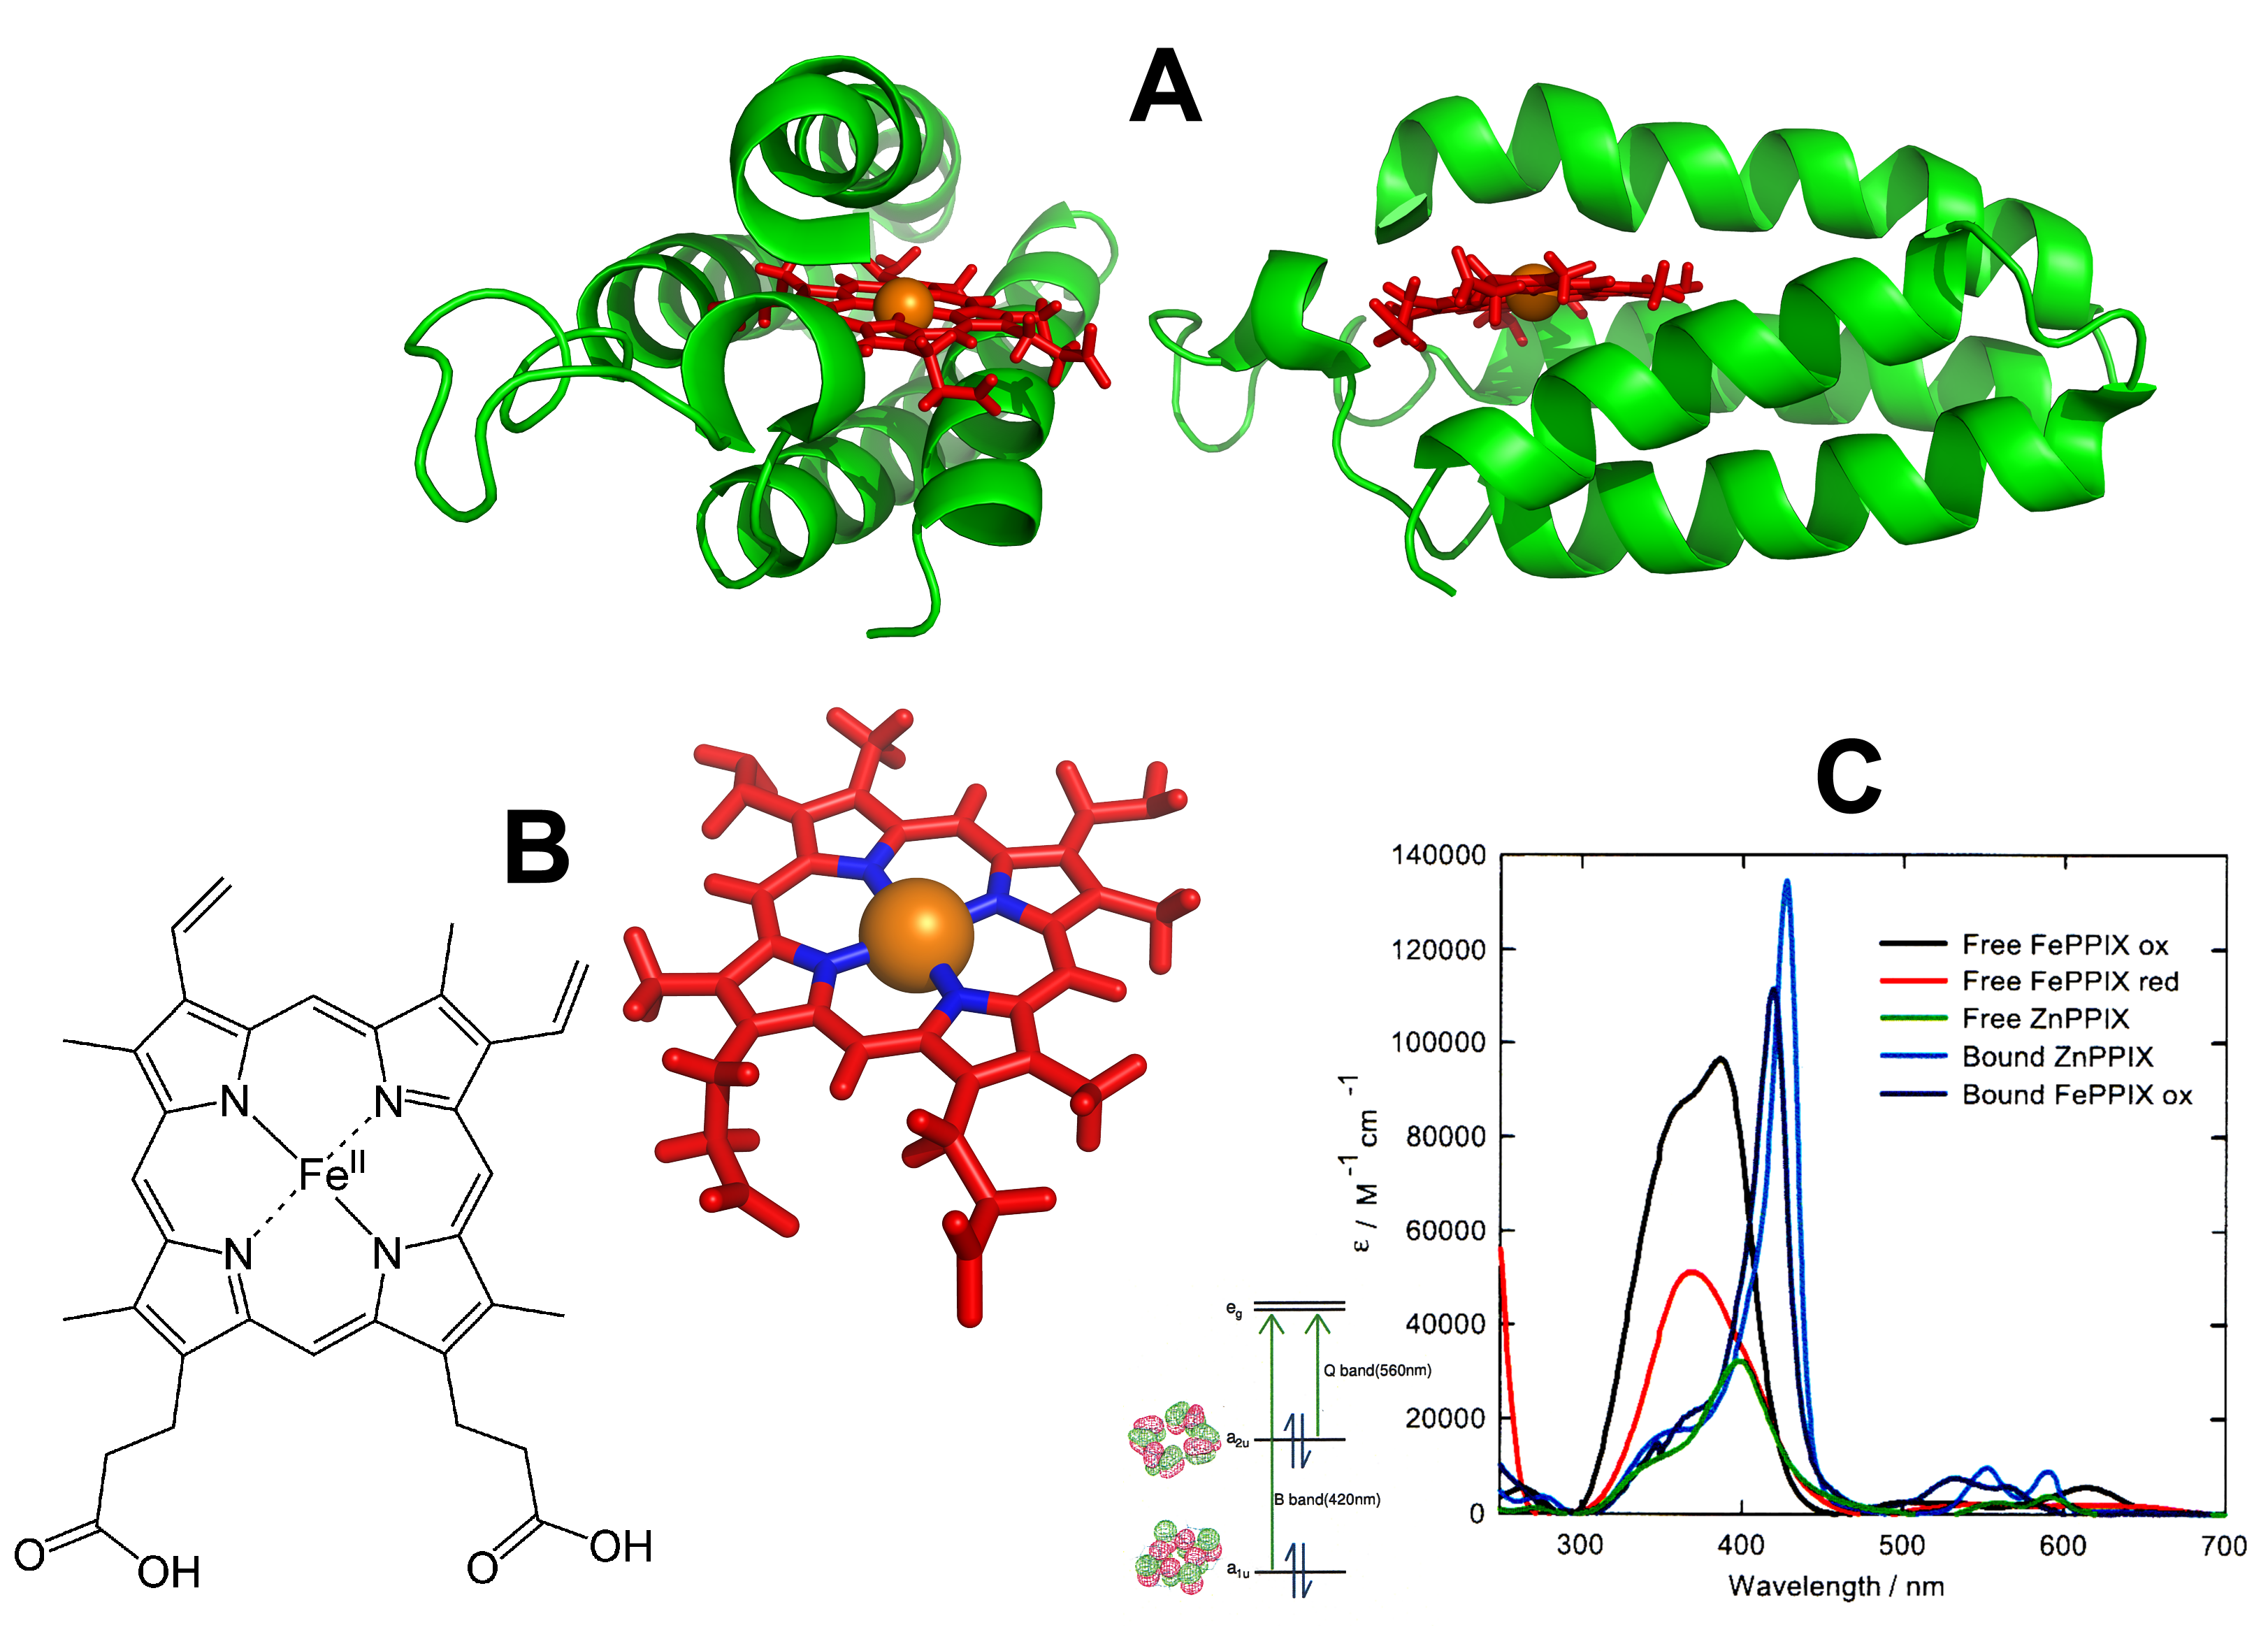
\includegraphics[width=137.4mm]{Images/haemStructure.png}
	\caption[Haem Structure]{A fancy image.}
	\label{fig:haemStructure}
\end{figure}
\end{verbatim}

\vspace{2ex}

\begin{figure}[!th]
	\centering
	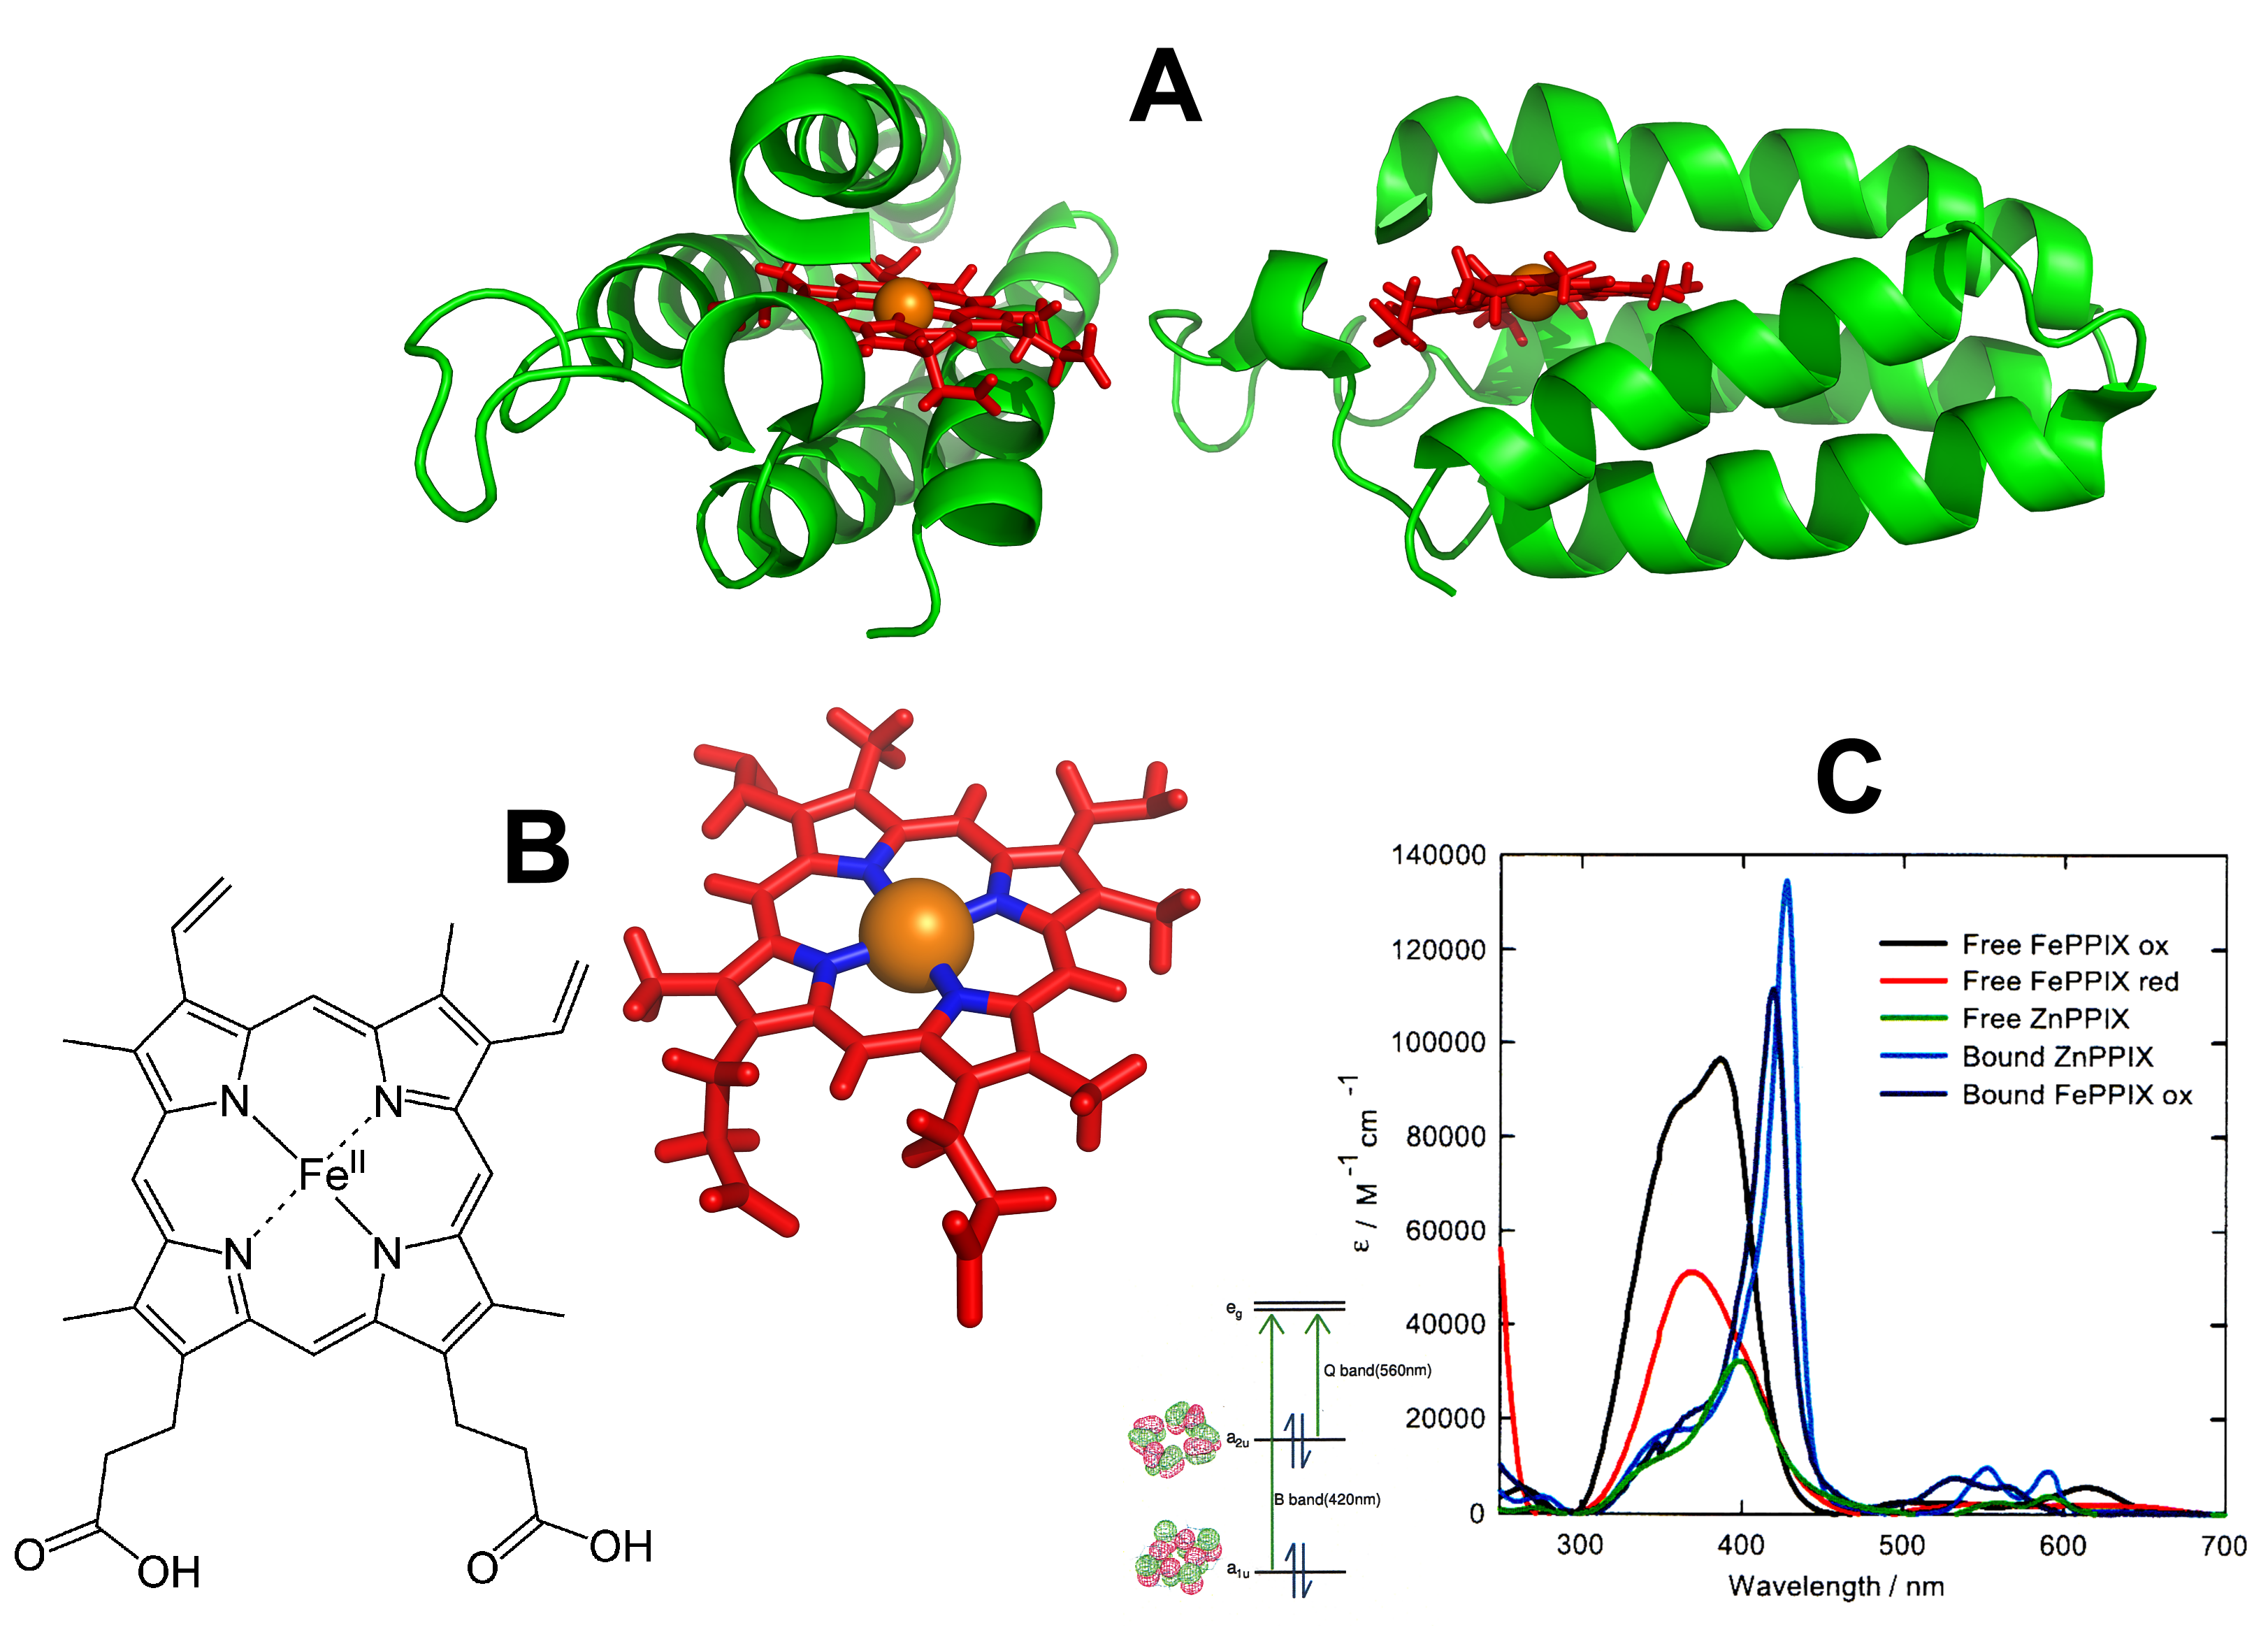
\includegraphics[width=137.4mm]{Images/haemStructure.png}
	\caption[Haem Structure]{A fancy image from Chris' Thesis.}
	\label{fig:haemStructure}
\end{figure}

In this example the command {\textbackslash}includegraphics tells LaTeX to look in the directory `Images' and incorporate the file called `haemStructure.png' into the final document while setting the width to 137.4mm.  This command can be used to resize a graphical file using the height or width parameter as shown. You must specify the units which can be pt, ex, em, mm, cm and so on. LaTeX recognises a very wide variety of standard units and graphics formats. The command is part of the graphicx package and so in the preamble you must include the command {\textbackslash}usepackage\{graphicx\}.

Many packages have been written to provide new commands. For example the `subfigure' package enables you to place separate images or files in the same figure side by side while giving them their own label. However, in this document we only concentrate on the very basics.

\section{Floating Environments}

Both tables and figures are examples of a `floating environments' which means LaTeX decides where to put them. 

The mysterious [!tbh] letters give guidance to LaTeX about roughly where the figure or table is  allowed to be, but in general they can move a long way from where you position them within your text file.  The letters in the square bracket can be t, h or b which stand for top, here or bottom.  If you don't specify any letters LaTeX defaults to [t].

LaTeX will always preserve the order in which figures appear.  If it cannot find a type setting solution, then it may move the float to it's own page, and combine it with other figures. If it still can't fit that in for some reason then it moves the float to the end of the document.  This has the effect of pushing all the remaining floating environments to the end of the document also.

The exclamation mark instructs LaTeX to ``try harder'' at putting the float where you told it to. Often you must play around to ensure the float positioning is acceptable, but usually this can be achieved by stretching or shrinking the image slightly using the size parameter, re-ordering text, judicial applications of the {\textbackslash}pagebreak command or by shouting loudly and slapping the computer monitor about. Note that it is better to resize the image using the original program that was used to create the image. Also using vector graphics can assist be useful (e.g. eps files) because they are designed to scale better.
\chapter{The Chapter on Making Chapters}
\label{sec:Chapters}

Right. LaTeX forces you to structure your document. There a series of simple commands for achieving this:

\vspace*{2ex}

{\textbackslash}chapter\{chapterName\}

{\textbackslash}section\{sectionName\}

{\textbackslash}subsection\{subsectionName\}

{\textbackslash}subsubsection\{subsubsectionName\}

\vspace*{2ex}

Easy enough. At the start of each chapter or section just issue one of these commands to name the section and LaTeX will present the chapter heading in the right style of font, which will be the same style of all the other heading names at that level of hierarchy throughout the document. In addition LaTeX assigns a number to that section. For example, this chapter was created using the command:

\vspace*{2ex}

{\textbackslash}chapter\{The Chapter on Making Chapters\} 

\vspace*{2ex}

LaTeX assigns the correct chapter number to each chapter in turn and then puts it in the table of contents, as you can see by looking at the table of contents! Easy.

\pagebreak
\section{The Section About Sections}
\label{sec:Section}
I think you're getting the hang of this. This section was created using the command {\textbackslash}section\{The Section About Sections\}. It appears in the table of contents as section \ref{sec:Section}.

\subsection{The Sub-Section About Sub-Sections}
\label{sec:SubSection}
Now you're really getting the hang of this. This subsection was created using the command {\textbackslash}subsection\{The Sub-Section About Sub-Sections\}. 

\subsubsection{The Sub-Sub-Section About Sub-Sub-Sections}
\label{sec:SubSubSection}
Now you're really getting the hang of this. but.. caught you out! This subsubsection doesn't have a number!  Ha Ha! It was created using the command {\textbackslash}subsubsection\{The Sub-Sub-Section About Sub-Sub-Sections\} in the same vein as all the other subsections/chapters etc. Here we have stopped the depth of the section numbering at the second level with the command:

\vspace*{2ex}

{\textbackslash}setcounter\{secnumdepth\}\{2\}

\vspace*{2ex}

Easy. WYSIWYM.  LaTeX does what you tell it to do. This is both a blessing and a curse.

\pagebreak
\section*{The Section About Sections That Don't Appear in the Table of Contents}
\label{sec:InvisibleSection}
Ok. Now we're throwing a spanner in the works. This section was created using the command:

\vspace*{2ex}

{\textbackslash}section*\{The Section About Sections That Don't Appear in the Table of Contents\}. 

\vspace*{2ex}

Notice how LaTeX has not assigned a number to the section and it doesn't appear in the table of contents. The effect of the * is to suppress the inclusion of a chapter, section or subsection in the automatic numbering. Easy. You can do this at any level. This is useful for things like prefaces, tables of contents or acknowledgements which you may or may not wish to have an entry in the main contents table. Up to you. It's your thesis. Don't just copy me.

\section{A Small Point About Numbering}

In this section notice how the numbering starts from where it left off before we suppressed the numbering on the previous section. Easy. WYSIWYM.
\pagebreak
\section{The Section About Internal Referencing}
\label{sec:InternalReferencing}

There are two related commands:

\vspace*{2ex}

{\textbackslash}label\{labelName\} 

{\textbackslash}ref\{labelName\}

\vspace*{2ex}


The {\textbackslash}label\{\} command allows you to create a label in a particular environment\footnote{That's right. Chapters, Sections and sub-sections etc are environments!}. The label won't appear in the final document. It's just a label which makes it easy to refer back to any particular environment elsewhere in the document. The {\textbackslash}ref\{\} command enables you to insert a reference anywhere in the document to any label in the document.  For example this is section \ref{sec:InternalReferencing}. The names you use in a label can be anything you like but musn't contain whitespace or special characters. I used the two commands:

\vspace*{2ex}

{\textbackslash}label\{sec:InternalReferencing\}

{\textbackslash}ref\{sec:InternalReferencing\}.

\vspace*{2ex}

The astute among you will realise that LaTeX has to read the document several times. Once to find the labels and then again to populate the references with the correct numbers. So you have to compile a latex document twice to get the referencing right. If there is a missing label or you refer to something that doesn't exist then latex inserts a convenient ? at that point. So hunting for queries is useful way of finding broken references. Latex issues warnings when it finds broken references.

As you create a document you will find yourself putting labels in all over the place so choose a sensible naming convention to help you remember the label names.

Each type of environment (equations, figures, tables, sections etc) has its own independent numbering system.  So when you choose your label name it's a good idea to have an identifier for that type of environment.  I have my own convention for label names which I use to help me remember references. E.g.   sec:SectionAboutCats. Eqn:EquationAboutCats,  Fig:FigureAboutCats and so on. This means you can differentiate between referring to the section or the figure more easily, even though they are about the same thing.

So Internal Referencing is a doddle. Easy!
\chapter{External Referencing}

Referencing is usually performed using a separate program called BibTex.  This program understands the file format .bib.

To create a reference within your document first you must create a .bib file by exporting your list of references from which ever referencing software you used, such as endnote, mendeley or whatever you use.

You can refer to an entry in the .bib file using the {\textbackslash}cite\{ref:Name\} command. the identifier `ref:Name' is the unique identifier which is the first line of each item included in your bibliography file.

For example, open the file LaTexCourseBib.bib in the bibliography directory. The first entry has the identifier `Horcas2007'.  This can be invoked as follows:


\begin{verbatim}
For example, this interesting fact\cite{Horcas2007}, is a cracking example.
\end{verbatim}

For example, this interesting fact\cite{Horcas2007}, is a cracking example.

During compilation latex and bibtex co-operate. During the first compilation latex generates a list of references that it needs.  During the second compilation bibtex populates the details from the .bib file into a shorter, ordered .bib file. The third compilation inserts markers at the right place in the main file and the fourth compilation generates the final list of references. Thus the compilation sequence is latex, bibtex, latex, latex.

The style of the referencing format can be changed using the command {\textbackslash}bibliographyStyle\{\}. e.g. the style used in this document is cjfthesisv1.bst which is invoked by 

\begin{verbatim}
\bibliographystyle{Bibliography/cjfthesisv1}
\end{verbatim}

The location of the list of references in the document is specified by issuing the {\textbackslash}bibliography\{\} command which also specifies the master bibliography file.

\begin{verbatim}
\bibliography{Bibliography/LaTeXCourseBib}
\end{verbatim}




\chapter{Organising Your Files}
One of the drawbacks of word is that the figures and tables are included within the document which becomes very very clunky quite quickly and once it reaches around 100Mb it becomes unwieldy and hard to export. One of that advantages of LaTeX is that the files are all text files and so are very light on resources and are easy to email around the place.

However, sometimes it can be difficult to navigate through a single text file, so if you had a huge document then it becomes difficult to find your way around.  One way of circumnavigating this problem is to break the file up into smaller files. As long as LaTeX knows where to look you can have a file for each logical sub-division of your document.

Therefore it is worth spending a bit of time at the beginning of a large project deciding how you wish to break up your LaTex Files and organise them neatly and tidily.  You can then tell LaTex where to look for the files using the following command:

\vspace*{2ex}
{\textbackslash}include\{fileName\}
\vspace*{2ex}

\pagebreak
\section{Linking a File}
We are now going to copy part of the tutorial file into a separate files and link it the main file.  Because this could go wrong it is sensible to back up tutorial.tex as something else. So save a copy called `tutorialOriginal.tex' for safe keeping. Then follow the following instructions.

\begin{enumerate}
\item Create a new file called MyFirstPage.tex
\item Select and Cut out the first chapter of Tutorial.Tex
\item Paste the first chapter into MyFirstPage.tex
\item Save both tutorial.tex and MyFirstPage.tex
\item Then add {\textbackslash}include\{MyFirstPage\} in tutorial.tex where the text used to be before you cut it out. We don't need to add the `.tex' because LaTeX can only include `.tex' files.
\item compile tutorial.tex and view the PDF
\end{enumerate}

The final PDF should look exactly the same as it was! except we now have a separate file for one of the chapters.

\pagebreak
\section{Creating A Class File}
We can also save our preamble in a separate file called a class file. This makes your main document much easier to understand.  To make it work we need to use the {\textbackslash}LoadClass\{\} command as follows: 

\begin{enumerate}
\item Create another new file and save it as TutorialStyle.cls
\item Copy the preamble of tutorial.tex into the new file. Starting with the {\textbackslash}documentclass{} command and copy right up to, but not including, the {\textbackslash}begin{document} command. Delete the preamble in the original document.
\item Save TutorialStyle.cls and tutorial.tex
\item Modify the first line of TutorialStyle.cls by replacing the word `document' with the word `Load'.
\item Add a new first line of tutorial.tex to use your new style class {\textbackslash}documentclass\{TutorialStyle\}
\item Save both files.
\end{enumerate}

\subsection{Sanity Check}

The first line of TutorialStyle.cls should now be:

\begin{verbatim}
\LoadClass[12pt, oneside, a4paper]{book}
\end{verbatim}
\vspace{2ex}

The first line of tutorial.tex should be:

\begin{verbatim}
\documentClass{TutorialStyle}
\end{verbatim}
\vspace{2ex}

We have just created what is called a style file. You can use this style file as a generic preamble for other documents as well. Compile tutorial.tex.  Nothing should have changed in the final PDF.


\pagebreak
\section{The Structure of this Document}

Lets now look at how I've organised this document. It is identical to my thesis because it started out life as my thesis. I usurped the structure and simply replaced the headings and content to make a kind of reference manual for this introductory course. This document therefore is three things:

\begin{enumerate}
\item An example thesis structure to work from.
\item The LaTeX files which were used to create it can be used as a template for a thesis.
\item It is also a convenient introductory latex manual!
\end{enumerate}

\vspace*{2ex}
Groovy huh?

\section{The Master File}

There is a master file where LaTeX begins the compilation procedure. This contains the {\textbackslash}documentclass command needed to set the ball rolling. Within the file there are a series of {\textbackslash}include\{\} commands, one for each Chapter, which tell LaTeX where to find the files containing each chapter.

The subfiles cannot be compiled on their own because they do not contain the {\textbackslash}documentclass, {\textbackslash}begin\{document\} or {\textbackslash}end\{document\} commands. Lets us look in more detail at the master file and we will learn some new LaTeX commands.

\singlespacing
\pagebreak
\begin{verbatim}
\documentclass{Style/LatexCourseStyle}

\begin{document}
\setcounter{secnumdepth}{2}
\setcounter{tocdepth}{1}

\frontmatter
\onehalfspacing
\include{Frontmatter/Titlepage}
\include{Frontmatter/Declaration}
\include{Frontmatter/Acknowledgements}
\include{Frontmatter/Summary}
\include{Frontmatter/Abbreviations}
\tableofcontents
\listoftables
\listoffigures

\mainmatter
\renewcommand{\sectionmark}[1]{\markright{\thesection \ #1}{}}
\include{Chapters/Overview}
\include{Chapters/MyFirstPage}
\include{Chapters/Lists}
\include{Chapters/mathsEquations}
\include{Chapters/ChemicalEquations}
\include{Chapters/Tables}
\include{Chapters/Figures}
\include{Chapters/Sectioning}
\include{Chapters/externalReferencing}
\include{Chapters/ThesisTemplateMainFile}
%\include{Chapters/ChapterThatIsNotCompiled}

\appendix
%\include{Appendices/UsefulWebsites}

\singlespacing

\backmatter
\addcontentsline{toc}{chapter}{References}
\bibliographystyle{Bibliography/cjfthesisv1}
\renewcommand{\bibname}{References}
\bibliography{Bibliography/LatexCourseBib}

\end{document}
\end{verbatim}
\onehalfspacing
\pagebreak

\section{Analysing the Master File}
Let us go through this file and observe the new commands. Most of it is self-explanatory.

\begin{verbatim}
\documentclass{Style/LaTeXCourseStyle}
\end{verbatim}

This command tells latex that the document class is the one defined in the the style file ''LaTeXCourseStyle'', which is in the sub directory ''style''.  Easy.

\begin{verbatim}
\setcounter{secnumdepth}{2}
\setcounter{tocdepth}{1}
\end{verbatim}

The first of these commands tells latex that the section depth number is 2. I.E. throughout the document only bother numbering sections, subsections and subsubsections down to the second level (such as section 1.2.3). The second command tells latex to only build the table of contents from section numbers down to the first level i.e. 1.1.  Easy enough.

The command {\textbackslash}frontmatter is exclusive to the book class, on which this style is based, and tells latex that within this section to number the pages using roman numerals, and not to include these numbers in the table of contents, just like in a book. The {\textbackslash}mainmatter and {\textbackslash}backmatter commands similarly delineate the other sections of the document.  

Childs play.  How long would it take you to figure out how to do that in word???? No idea. I've never tried.

Note that these rather cool commands are not available in every single class. So for a paper you would use the article class where such compartmentalisation of your document is not appropriate. In fact you can often download latex templates from the journal to wish to submit your paper, which is why I concentrate on the thesis template in this course.

\begin{verbatim}
\onehalfspacing
\end{verbatim}

Is obvious. ''From this point forward use line spacing of one and a half lines please. Thank you.'' How many hours have you spent clicking on paragraph indentations for each separate paragraphs in word? Nightmare. Want to change the standard in the whole document? Not a chance in word. In latex, you can do it with a single word, carefully placed in the master file.

\begin{verbatim}
\include{Frontmatter/Titlepage}
\include{Frontmatter/Declaration}
\include{Frontmatter/Acknowledgements}
\include{Frontmatter/Summary}
\include{Frontmatter/Abbreviations}
\end{verbatim}

The {\textbackslash}include\{\} command tells latex to include the specified .tex file at this point.  Thus it is a simple matter to break up a large document into sub components.  I have written each part of the front matter in a separate file and then grouped all the front matter into one directory called: Frontmatter.

See how the directory structure of my files reflects the structure of my book?

\begin{verbatim}
\tableofcontents
\listoftables
\listoffigures
\end{verbatim}

Again. This is easy. These commands mean: ''Please scan through the whole document and build for me a table of contents, a list of tables, a list of figures and then write down the entries along side their section numbers (as I have them ordered in this version of the document), as well as the page numbers on which they appear and create a nice little summary table and add them to the front matter of my document. Thanks.''.

How does latex do this?  remember the idea of environments?  Well each table, figure, equation etc is a defined environment.  LaTeX just counts them up and assigns numbers starting wherever you want and builds a table.  You can tell latex to ignore individual sections if you want to.

You can also control the look and feel of your table of contents with subtley and grace. Do you want to fill the white space with lines of dots to aid readability, even though the chapter titles are all different lengths? page numbers? How deep should the TOC been?  etc etc etc. How to do this is beyond the scope of this course, but now you know about it, go look it up. easy as $\pi$.

Ok.

Main matter we've done.

\begin{verbatim}
\renewcommand{\sectionmark}[1]{\markright{\thesection \ #1}{}}
\end{verbatim}

This command tells latex to 'renewcommand', i.e. change the meaning of the following command from this point in the document forward, over-riding previous definitions.
\begin{verbatim}
\sectionmark}[1]{\markright{\thesection \ #1}{}
\end{verbatim}

Is latex speak for ``please write the section heading at the top right hand side of each page. thanks''. This works in conjunction with a command in the style file which we'll talk about later. You have to tell latex to switch on headings as well as where to put them.

\begin{verbatim}
\include{Chapters/Overview}
\include{Chapters/MyFirstPage}
\include{Chapters/Lists}
\include{Chapters/mathsEquations}
\include{Chapters/ChemicalEquations}
\include{Chapters/Tables}
\include{Chapters/Figures}
\include{Chapters/Sectioning}
\include{Chapters/externalReferencing}
\include{Chapters/ThesisTemplateMainFile}
%\include{Chapters/ChapterThatIsNotCompiled}
\end{verbatim}

This is the include command again. You will notice that one of the include lines is commented out. This is a handy trick to only build certain parts of my thesis. Which can be useful if individual chapters are being reviewed.

\pagebreak

\begin{verbatim}
\appendix
%\include{Appendices/UsefulWebsites}

\singlespacing

\backmatter
\addcontentsline{toc}{chapter}{References}
\bibliographystyle{Bibliography/cjfthesisv1}
\renewcommand{\bibname}{References}
\bibliography{Bibliography/LatexCourseBib}
\end{verbatim}

The rest is easy. {\textbackslash}Appendix means we are in the appendix now and start labelling sections with A.1.2 instead of 1.2.3.  

{\textbackslash}addcontentsline means forcibly insert a contents line about the references into the contents table. 

{\textbackslash}\{bibliographystyle\{Bibliography/cjfthesisv1\}\} means use the biblography style defined in the file cjfthesisv1. Defining a bibliography style will be covered later if we have time. This is where you specify how the references will appear (names, journals, full stops, commas etc).

{\textbackslash}renewcommand\{{\textbackslash}bibname\}\{References\} means: rename the bibliography chapter as `References'

{\textbackslash}biblography means add the following bibliography.  You can reference entries in this bibliography file very easily.

The astute among you will realise that LaTeX will have to read the document several times before it can be compiled with all the references.  Hey ho. No problem. You can go and have a cuppa while LaTeX does your references for you in the style of your favorite journal... nice.




%\include{Chapters/ChapterThatIsNotCompiled}

\appendix
%\include{Appendices/UsefulWebsites}

\singlespacing

\backmatter
\addcontentsline{toc}{chapter}{References}
\bibliographystyle{Bibliography/cjfthesisv1}
\renewcommand{\bibname}{References}
\bibliography{Bibliography/LatexCourseBib}

\end{document}
\end{verbatim}
\onehalfspacing
\pagebreak

\section{Analysing the Master File}
Let us go through this file and observe the new commands. Most of it is self-explanatory.

\begin{verbatim}
\documentclass{Style/LaTeXCourseStyle}
\end{verbatim}

This command tells latex that the document class is the one defined in the the style file ''LaTeXCourseStyle'', which is in the sub directory ''style''.  Easy.

\begin{verbatim}
\setcounter{secnumdepth}{2}
\setcounter{tocdepth}{1}
\end{verbatim}

The first of these commands tells latex that the section depth number is 2. I.E. throughout the document only bother numbering sections, subsections and subsubsections down to the second level (such as section 1.2.3). The second command tells latex to only build the table of contents from section numbers down to the first level i.e. 1.1.  Easy enough.

The command {\textbackslash}frontmatter is exclusive to the book class, on which this style is based, and tells latex that within this section to number the pages using roman numerals, and not to include these numbers in the table of contents, just like in a book. The {\textbackslash}mainmatter and {\textbackslash}backmatter commands similarly delineate the other sections of the document.  

Childs play.  How long would it take you to figure out how to do that in word???? No idea. I've never tried.

Note that these rather cool commands are not available in every single class. So for a paper you would use the article class where such compartmentalisation of your document is not appropriate. In fact you can often download latex templates from the journal to wish to submit your paper, which is why I concentrate on the thesis template in this course.

\begin{verbatim}
\onehalfspacing
\end{verbatim}

Is obvious. ''From this point forward use line spacing of one and a half lines please. Thank you.'' How many hours have you spent clicking on paragraph indentations for each separate paragraphs in word? Nightmare. Want to change the standard in the whole document? Not a chance in word. In latex, you can do it with a single word, carefully placed in the master file.

\begin{verbatim}
\thispagestyle{empty}

\begin{center}
\vspace*{\stretch{1}}

\hrule height 2pt
\vspace*{2ex}
{\Huge\textbf{Towards the Ability to Make Super Duper LaTeX Documents}\par}
\vspace*{2ex}
\hrule height 2pt
\vspace*{10ex}
{
\includegraphics[height=40mm]{Images/UnivShield}\par}
\vspace*{10ex}
{\large\textbf{Christopher~James~Forman}\par}
\vspace*{2ex}
{\large{Department Of Chemistry}\par}
\vspace*{2ex}
{\large{University of Cambridge}\par}
\vspace*{5ex}
{\large{This dissertation is submitted for the degree of \textit{Doctor of Philosophy}}\par}
\vspace*{5ex}
{\large{\today}\par}

\vspace*{\stretch{2}}
\end{center}
\chapter*{Declaration}

\vfill

This dissertation is the result of my own work and includes nothing which is the outcome of work done in collaboration except where specifically indicated in the text. It is not substantially the same as any that I have submitted for a degree or diploma or other qualification at any other University and no part has already been, or is concurrently being, submitted for any degree, diploma, or other qualification. It does not exceed 60,000 words, including tables, footnotes, bibliography and appendices.\par

\vspace{10ex}

\begin{flushright}
Signature: \rule[0pt]{60mm}{0.5pt}

\vspace{5ex}

Date: \rule[0pt]{60mm}{0.5pt}
\end{flushright}

\vfill
\chapter*{Acknowledgments}
\subsection*{Family}
Mum. Dad. Pet Dog.

\subsection*{Scientific Collaborations}
Dr A.N.Other at uni of blah for samples and instrument time etc. My Amazing Lab Chums.

\subsection*{Scientific Support}
My amazing lab chums.

\subsection*{General Assistance}
Cleaner, My amazing lab chums.

\subsection*{Financial Support}
Bank, Tax payer. My amazing lab chums.

\subsection*{Moral Support}
My Amazing Lab chums.

\subsection*{Academic Inspiration}
Netwon, My super. My Amazing Lab Chums.

\subsection*{Everyone else}
My Amazing Lab Chums.

\chapter*{Summary}
This document is a handbook for introducing you to LaTeX. It contains a bit of background about the history and philosophy of LaTeX.  However, it concentrates on providing a guided practical introduction to the basic techniques such as 
\begin{itemize}
\item Lists
\item Mathematical and chemical equations
\item Tables
\item Figures
\item Chapters and Sections
\item Linking to other files in large documents
\item Referencing
\end{itemize}

The handbook is also presented in the style of a thesis. This means that source files provided on the introductory course and available from the department web page are a convenient template for a thesis.

More details on specific aspects of LaTeX can be found at the departmental LaTeX page which can be found here:

 http://www-ch-int.ch.private.cam.ac.uk/latex/about

\chapter*{Abbreviations}

\begin{longtable}{r >{\rule{0pt}{3ex}}l<{\rule[-1.5ex]{0pt}{0pt}}}
ADP & Adenosine Diphosphate\\
(nc/c)AFM & (non-contact/conducting) Atomic Force Microscopy\\
ATP & Adenosine Triphosphate \\
\end{longtable}
\end{verbatim}

The {\textbackslash}include\{\} command tells latex to include the specified .tex file at this point.  Thus it is a simple matter to break up a large document into sub components.  I have written each part of the front matter in a separate file and then grouped all the front matter into one directory called: Frontmatter.

See how the directory structure of my files reflects the structure of my book?

\begin{verbatim}
\tableofcontents
\listoftables
\listoffigures
\end{verbatim}

Again. This is easy. These commands mean: ''Please scan through the whole document and build for me a table of contents, a list of tables, a list of figures and then write down the entries along side their section numbers (as I have them ordered in this version of the document), as well as the page numbers on which they appear and create a nice little summary table and add them to the front matter of my document. Thanks.''.

How does latex do this?  remember the idea of environments?  Well each table, figure, equation etc is a defined environment.  LaTeX just counts them up and assigns numbers starting wherever you want and builds a table.  You can tell latex to ignore individual sections if you want to.

You can also control the look and feel of your table of contents with subtley and grace. Do you want to fill the white space with lines of dots to aid readability, even though the chapter titles are all different lengths? page numbers? How deep should the TOC been?  etc etc etc. How to do this is beyond the scope of this course, but now you know about it, go look it up. easy as $\pi$.

Ok.

Main matter we've done.

\begin{verbatim}
\renewcommand{\sectionmark}[1]{\markright{\thesection \ #1}{}}
\end{verbatim}

This command tells latex to 'renewcommand', i.e. change the meaning of the following command from this point in the document forward, over-riding previous definitions.
\begin{verbatim}
\sectionmark}[1]{\markright{\thesection \ #1}{}
\end{verbatim}

Is latex speak for ``please write the section heading at the top right hand side of each page. thanks''. This works in conjunction with a command in the style file which we'll talk about later. You have to tell latex to switch on headings as well as where to put them.

\begin{verbatim}
\chapter{Overview}
\label{chap:overview}
\section{LaTeX: The answer to everything.}
LaTeX is typsetting program that takes an input file of marked up text and then, with a user defined set of rules, typesets a beautifully crafted output file that can be easily printed (e.g. a pdf). 

\subsection{Advantages}

The advantages of this method are manifold:

\begin{itemize}

\item Use any text editor to view the source document.
\item More time can be spent working on the content and not worrying about how text or figures interact in the layout until later on.
\item LaTeX uses consistent rules throughout a document
\item LaTeX sorts out basic typesetting automatically
\item Changes can be introduced globally with very little effort
\item Document structure is explicit
\item Documents can be professionally typeset and look great
\item You are forced to structure your documents correctly.
\item Mathematical equations, like $E=mc^2$ or $\imath\hbar\frac{\partial}{\partial t}\Phi (x, t) = \hat{H}\Phi (x, t)$ can be produced almost as fast as typing (if you know the commands!).
\end{itemize}

\subsection{Disadvantages}
The disadvanatges of this method are also manifold:
\begin{itemize}
\item You don't see the output as you go.
\item Steep learning curve.
\item Documents are harder to edit by a second author (unless they are adept at LaTeX too). This can be mitigated using version control, which makes group authoring processes superior to word.
\item The program never works quite the way you want it to and learning how to influence it can be problematic and subtle.
\item Although intended to save work the principle of 'conservation of work' means that you simply transform problems associated with WYSISYG approaches to problems associated with WYSIWYM approaches!
\item You can go blind trying to determine the difference between wiggly and smooth brackets if your editors font isn't large enough.
\end{itemize}

\subsection{On balance?}
If it's so rubbish, why use LaTeX?

\begin{itemize}
\item Large documents are much more easily handled. 
\item In general it is quicker to debug a LaTeX document than typeset an entire thesis manually. 
\item Technical information such as tables, equations and figures are integrated much more smoothly than with word.
\end{itemize}

\section{How does it work?}

The raw text is interspersed with commands, preceded by a \textbackslash, which tell LaTeX what to do with the text. For example you can \textbf{make it bold}, \emph{italic}, or \underline{underlined} with the commands {\textbackslash}textbf\{\}, {\textbackslash}emph\{\} or {\textbackslash}underlined\{\}. More on commands in a moment...



\chapter{My First Page}

\section{The Very Beginning}
The very simplest LaTeX document might look like this:

\begin{verbatim}
\documentclass[a4paper,12pt]{article}
\begin{document}
Hello World.
\end{document}
\end{verbatim}

\pagebreak
\thispagestyle{empty}
Hello World.
\pagebreak
\subsection{Break Down}
What's all the gobbledegook around my simple message???

In LaTeX we intersperse text and commands.  Commands are preceded by a \textbackslash. For example the first line in a LaTeX document \underline{\textbf{\emph{must}}} be:

\begin{verbatim}
\documentclass[options]{class}
\end{verbatim}

Where the word ''class'' may be substituted for one of many things such as: article, proc, minimal, report, book, letter, memoir, slides, beamer.

Similarly, and completely generally in LaTeX speak, the square brackets denote the existence of optional parameters. Each individual command can take its own parameters and for the ''{\textbackslash}documentclass'' command there are options for controlling font size, font family, landscape, oneside, twosided, page size and so on. These options will persist throughout the entire document. For example the document class command for this document, (which is likely to be like the one you would use for a thesis), would be:

\begin{verbatim}
\documentclass[12pt, oneside, a4paper]{book}
\end{verbatim}

Other options include:

\begin{itemize}
\item {10pt, 11pt, 12pt (default is 10pt).}
\item {letterpaper, legalpaper, a4paper, executivepaper, a5paper, b5paper}
\end{itemize}
and so on.

\pagebreak
\section{Can I start typing please?}

After we have set up the document we can start actual work on our document. So we must tell LaTeX that what follows is to be interpreted as a document.  The command {\textbackslash}begin can take many different parameters and is a command to enter what is known, in LaTeX speak, as 'an environment'. Thus the commands:
\begin{verbatim}
\begin{document}

\end{document}
\end{verbatim}

tells LaTeX to enter and leave the document environment, and thus constitute the outer limits of our document file. Other environments include the equation environment, the itemize environment, the figure environment and so on. These will be encountered in due course.

Every part of the LaTeX file is therefore within an environment of specific type and the content within each environment consists of commands or text.

That's basically it.

So let's get on with it shall we...

\pagebreak
\section{The ground rules}
\begin{quote}
Hold on, hold on, hold on my son.

First the lessons.

Then the fun!
\end{quote}
Dr Seuss.

\subsection{Spaces}
Whitespace characters, such as blank or tab, are treated uniformly as space by LaTeX. Several consecutive whitespace characters are treated as one single space. Whitespace at the start of a line is generally ignored, and a single line break is treated as whitespace. An empty line between two lines of text defines the end of a paragraph. Several empty lines are treated the same as one empty line. The text below is an example.

\begin{verbatim}
It does not matter whether you
enter one or several             spaces
after a word. The final result will be typeset beautifully
according    to     precise rules.




An empty line starts a new
paragraph. Note the indentation on the first line of the paragraph, 
except at the beginning of the section. 
\end{verbatim}

\vspace*{2ex}
\vspace*{2ex}

It does not matter whether you
enter one or several             spaces
after a word. The final result will be typeset beautifully
according    to     specific rules.




An empty line starts a new
paragraph. Note the indentation on the first line of the paragraph, except at the beginning of the section. 

\pagebreak
\subsection{Special Characters}
The symbols 

\# \$ \% \textasciicircum{} \& \_ \{ \} \~{} \textbackslash

are reserved characters that either have a special meaning under LaTeX or are unavailable in all the fonts. If you enter them directly in your text, they will normally not print, but rather make LaTeX do strange things.

To overide the special meanings of these symbols and allow them to produced within your text you may use the following sequences:
\begin{verbatim}
\# \$ \% \textasciicircum{} \& \_ \{ \} \~{} \textbackslash
\end{verbatim}

Other symbols and many more can be printed with special commands in mathematical formulae or as accents.

The backslash character '\textbackslash' cannot be entered by adding another backslash in front of it ( \textbackslash\textbackslash); because this sequence means ''linebreak''.

The command \textbackslash\~{}\{\} produces a tilde which is placed over the next letter. For example \textbackslash\~{}\{n\} gives \~{n}. To produce just the character \~{}, use \textbackslash\~{}\{\} which places a \~{} over an empty box.

Similarly, the command \textbackslash\textasciicircum{} produces a hat over the next character, for example \textbackslash\textasciicircum\{o\} produces \^{o}.

\pagebreak
\section{Preamble}
After the {\textbackslash}documentclass command we add ''preamble''. Here we load special features that we will use throughout our document to expand on the basic capabilities of LaTex. These are contained in units called ''packages'' which we can tell our LaTeX compiler to download by using the command ''{\textbackslash}include\{packageName\}''. 

There are many repositories of such packages on the web. Your compiler generally knows where to look and most standard packages are included with any install. For example, to include a special set of typesetting instructions to handle chemical equations we can grow our simple document with a single command like this:

\begin{verbatim}
\documentclass[a4paper,12pt]{article}
\usepackage[version=3]{mhchem}
\begin{document}
Hello World!

We all need \ce{H2O}.

I'm less fussed about \ce{^{235}_{92}U+}.

\end{document}
\end{verbatim}

\vspace{2ex}

\pagebreak
\thispagestyle{empty}
Hello World!

We all need \ce{H2O}.

I'm less fussed about \ce{^{235}_{92}U+}.
\pagebreak

Here we have loaded a package called: "`mhchem"' which took the option ''[version=3]''. This is a package for drawing chemical equations easily and it has it's own instruction manual which you can follow easily. It is included in the bundle of files for this course.

Other things we can do in the premable within LaTeX are to redefine existing commands or create our own personal commands. These can be stored in a file called the 'style file' which we can load at the beginning of our document, in place of our documentclass. More about this later on...


\subsection{Comments}
It is often useful to comment your LaTeX documents. You can leave yourself amusing, sarcastic messages that won't get printed out in the final document. Use this to make your own notes as the course progresses.

To get a comment use the \% command, which tells LaTeX to ignore the rest of the line, the line break and all the white space at the beginning of the next line, for example, we may add to our continually evolving document...

\begin{verbatim}
\documentclass[a4paper,12pt]{article}
\usepackage[version=3]{mhchem}
\begin{document}
Hello World!

%All humans need water and I would like 
%to include this concept in my arguments.
We all need \ce{H2O}.

%Uranium 235 is toxic, which is why I don't want to consume it... 
I'm less fussed about \ce{^{235}_{92}U+}.

\end{document}
\end{verbatim}

\vspace{4ex}
Hello World!

%All humans need water and I would like to include this concept in my arguments.
We all need \ce{H2O}.

%Uranium 235 is toxic, which is why I don't want to consume it... 
I'm less fussed about \ce{^{235}_{92}U+}.

\pagebreak
\section{Compiling}
Once the document is finished you can compile it. Your compiler will depend on the platform that you use. In the PWF we are using winEDT to edit the documents (a LaTeX front end) and texlive2008 which is the compiler itself. I use MiKTex and the front end texCenter.  There is no need to use a front end. If you prefer you can use a simple text editor and a command line.

the recommended distributions are:
\begin{itemize}
\item MiKTeX or TeX Live for Windows
\item TeX Live for Unix/Linux
\item MacTeX or TeX Live for Mac OS.
\end{itemize}

Once you have installed your software and got it working, written your source code and tried to compile it, there will nearly always be something wrong with your file. 

Any errors will be highlighted in the console window or error output box of your front end.  Some front ends dump the running commentary which LaTeX produces into a text file for easy reading afterwards.

In a compile attempt (successful or otherwise) LaTeX may produce the following files:

projectname.aux

projectname.bbl

projectname.lof

projectname.lot

projectname.txt

projectname.toc

projectname.dvi

These are interim files (toc= table of contents, bbl = bibliography etc). To be honest I have no idea what half of these things contain.  You only need the .tex file and a compiler with the right packages installed to produce them again.

Some versions of LaTeX only produce DVI files and you then need to convert the dvi file to a PDF or download a dvi viewer. You can also convert DVI files to PS files and then view them.  The good thing about front ends is that you can set them up to produce PDFs directly.

OK. So we have now produced a silly document but we understand it.  Now lets get on with learning how to make our own documents.



\chapter{Lists}
Lists are great.  The command {\textbackslash}begin\{\} can be used to enter a list environment.  For example:

\begin{verbatim}
\begin{itemize}
\item cat
\item dog
\item horse
\end{itemize}
\end{verbatim}

Produces:

\begin{itemize}
\item cat
\item dog
\item horse
\end{itemize}

\pagebreak
We can also replace the bullet points with numbers using the enumerate keyword.

\begin{verbatim}
\begin{enumerate}
\item cat
\item dog
\item horse
\end{enumerate}
\end{verbatim}

\begin{enumerate}
\item cat
\item dog
\item horse
\end{enumerate}

\pagebreak
and we can use the description keyword which does this:
\begin{verbatim}
\begin{description}
\item[Cat] a lovely furry creature with a cute nose and whiskers.
\item[Dog] Another furry creature that smells rather well; 
           its olfactory power stems from its nasal dampness.
\item [Horse] A large stinky creature with sideways facing eyes.
\end{description}
\end{verbatim}

\begin{description}
\item[Cat] a lovely furry creature with a cute nose and whiskers.
\item[Dog] Another furry creature that smells rather well; its olfactory power stems from its nasal dampness.
\item [Horse] A large stinky creature with sideways facing eyes.
\end{description}
\chapter{Maths Equations}

\section{Producing Beautiful Looking Mathematics}

One of the best features about LaTeX is `maths mode'.  For example the schrodinger equation can be produced as follows:

\vspace*{2ex}

\begin{center}
\begin{math}
\imath\hbar\frac{\partial}{\partial t}\Phi (x, t) = \hat{H}\Phi (x, t)
\end{math}
\end{center}

\vspace*{2ex}

\begin{verbatim}
\begin{math}
\imath\hbar\frac{\partial}{\partial t}\Phi(x,t)=\hat{H}\Phi(x,t)
\end{math}
\end{verbatim}

There are a number of ways to switch on maths mode.  The first, as above, is with the {\textbackslash}begin\{math\} environment. You can also enter mathmode inline using the \$ symbol. For example typing in \$y=ax\textasciicircum{}2+bx+c\$ yields $y=ax^2+bx+c$.  Another way is to enter the equation environment which enables you to number equations so you can then refer to them later in the text.

\begin{equation}
y(t)= \sin \left(\frac{{\alpha}t}{2\pi} + \phi_0\right)
\label{eqn:MadeUpNonsense}
\end{equation}

\vspace*{2ex}
\begin{verbatim}
\begin{equation}
y(t)= \sin \left(\frac{{\alpha}t}{2\pi} + \phi_0\right)
\end{equation}
\end{verbatim}.

\section{Basic Maths Mode}
Once in maths mode there is a kind of text based code for writing down your equations.  Here are the most basic symbols to get you going.
\begin{center}
\begin{tabular}{cc}
\toprule
Final Result & LaTeX Code \\
\cmidrule(){1-2}
$a+b$ & a+b \\
$a-b$ & a-b \\
$ab$ & ab \\
$a*b$ & a*b \\
$a \times b$ & a {\textbackslash}times b \\
$a \cdot b$ & a {\textbackslash}cdot b \\
$\frac{a}{b}$ & {\textbackslash}frac\{a\}\{b\} \\ 
$a^b$ & a\textasciicircum{}b \\
$a_b$ & a\_b \\
$\sin a$ & {\textbackslash}sin a  (same for cos, tan)\\
$ sin a$ & sin a \\
$\sqrt{a}$ & {\textbackslash}sqrt\{a\} \\
$\left( a \right) $ & {\textbackslash}left( a {\textbackslash}right)\\ 
$\left[ a \right]$ & {\textbackslash}left[ a {\textbackslash}right]\\ 
$\alpha$ & {\textbackslash}alpha \\
$\pi$ & {\textbackslash}pi \\
\bottomrule
\end{tabular}
\end{center}

A full treatise on maths mode is not practical here. There are lots of online tutorials and summaries of symbols. It just takes a bit of practice and you can build up equations really easily. It's straight forward to learn new stuff once you've done it a few times.

\pagebreak
\section{Equation Arrays}
Sometimes you need to arrange several equations vertically, referencing individual lines separately and aligning the equations on the $=$ sign. This can be achieved with equation arrays as follows:

\begin{eqnarray}
A\left( x\right) & = & \frac{x^2+2x+1}{x+1} \\
& = & \frac{\left(x+1\right)\left(x+1\right)}{x+1} \nonumber\\
& = & x+1 \nonumber\\
B(x,t) & = & \frac{e^{\left(\imath\omega_0 t + kx\right)}}{4\pi\epsilon_0}
\end{eqnarray}

\begin{verbatim}
\begin{eqnarray}
A\left( x\right) & = & \frac{x^2+2x+1}{1+x} \\
& = & \frac{\left(x+1\right)\left(x+1\right)}{1+x} \nonumber\\
& = & x+1 \nonumber\\
B(x,t) & = & \frac{e^{\left(\imath\omega_0 t + kx\right)}}{4\pi\epsilon_0}
\end{eqnarray}
\end{verbatim}

\begin{itemize}
\item Note the \& symbols. This tells LaTeX where to align the equations. There must be the same number of \& symbols in each line.
\item Note the \textbackslash\textbackslash ~at the end of each line except the last one. This symbol tells LaTeX to add another row in the array.  If you put it on the last line you get an empty row at the bottom of the array.
\item Note the {\textbackslash}nonumber command which suppresses line numbering for that line.
\item Note that equation number carries on from equation \ref{eqn:MadeUpNonsense} in the previous section.
\end{itemize}

\section{Maths Packages}

Maths mode comes as standard in LaTeX, however you can download packages that buff up your maths symbol set. For example neat vector notation comes in the package `vector'. e.g. {\textbackslash}uuvec\{T\} yields $\uuvec{T}$.

\begin{verbatim}
\usepackage{amssymb}
\usepackage{amsmath}
\usepackage{vector}
\end{verbatim}


\chapter{Chemical Equations}
The mhchem package means you can do basic stuff very easily using {\textbackslash}ce\{\}. For example:

\vspace{2ex}
\begin{verbatim}
\ce{CO2 + C -> 2CO}
\ce{CO2 + C <- 2CO}
\ce{CO2 + C <=> 2CO}
\ce{A-B=C#D\sbond E\dbond F\tbond G}
\end{verbatim}
\vspace{2ex}
\begin{center}
\ce{CO2 + C -> 2CO}

\ce{CO2 + C <- 2CO}

\ce{CO2 + C <=> 2CO}

\ce{A-B=C#D\sbond E\dbond F\tbond G}
\end{center}

\vspace{2ex}
You can also use math mode within chemical equations.
\vspace{2ex}

\begin{center}
\ce{$x\,$ Na(NH4)HPO4 ->[\Delta] (NaPO3)_{$x$} + $x\,$ NH3 ^ + $x\,$ H2O}
\end{center}

\begin{verbatim}
\ce{$x\,$ Na(NH4)HPO4 ->[\Delta](NaPO3)_{$x$} + $x\,$ NH3 ^ + $x\,$ H2O}
\end{verbatim}

And you can number chemical reactions as well by using the math mode equation environment.

\begin{equation}
\ce{CO2 + C <=> 2CO}
\end{equation}

\begin{verbatim}
\begin{equation}
\ce{CO2 + C <=> 2CO}
\end{equation}
\end{verbatim}

However, this will number mathematical and chemical equations using the same number system. There is a discussion in the mhchem pdf which shows you how to number chemical and mathematical equations independently. It's a bit complex and involves you creating your own type of environment... bit beyond the intro level of this course...
\chapter{Tables}
Tables are big business in Latex.  I use these packages to help me.

\begin{verbatim}
\usepackage{multirow}
\usepackage{booktabs}
\usepackage{dcolumn}
\end{verbatim}

Here's an example table

\begin{table}[!hb]
 \centering
	\begin{tabular}{@{}rccc@{~}r@{.}l*3{r@{.}l@{~}r@{.}l}D{.}{\cdot}{2,1}}
	\toprule
	\multicolumn{1}{c}{Fibre Type}
	& N 
	& M 
	&\multicolumn{3}{c}{$L_t$ (nm)}
	&\multicolumn{4}{c}{$R_t$ (nm)}
	&\multicolumn{4}{c}{$d_t$ (nm)}
	&\multicolumn{4}{c}{${\Delta}Z_t$ (nm)}
	&\multicolumn{1}{c}{~}\\
\cmidrule(lr){1-1}
\cmidrule(lr){2-2}
\cmidrule(lr){3-3}
\cmidrule(lr){4-6}
\cmidrule(lr){7-10}
\cmidrule(lr){11-14}
\cmidrule(lr){15-18}
  SS Twisted & 5 & 4 & 313 &\multicolumn{2}{c}{(122)} & 5&7 &(1&6)  & 5&4 &(1&0)  &  150&5 &(63&1) &\multicolumn{1}{c}{~} \\
  \multicolumn{19}{c}{~}\\
  %\cmidrule(lr){3-18}
  &
  &
 	&\multicolumn{3}{c}{$L_s$ (nm)} 
 	&\multicolumn{4}{c}{$R_s$ (nm)}
 	&\multicolumn{4}{c}{$W_s$ (nm)}
 	&\multicolumn{4}{c}{${\Delta}Z_s$ (nm)}
 	&\multicolumn{1}{c}{${\Delta}Z_{e}$ (nm)}\\
\cmidrule(lr){4-6}
\cmidrule(lr){7-10}
\cmidrule(lr){11-14}
\cmidrule(lr){15-18}
\cmidrule(lr){19-19}
  SS Spiral& 32 & 7 &123&(31&6)&11&4&(3&3)&11&1&(2&6)&32&9&(22&2)&26.9\\
  SSB Spiral& 64&18 &106&(22&9)&10&8&(2&7)&9&8&(1&8)&28&2&(8&1)&22.7\\
	%\midrule
  BSS Spiral&37 &19 &110&(44&9)&13&4&(3&0)&12&9&(1&8)&27&1&(9&1)&21.5\\
	%\midrule
  SSSB Spiral&26& 6 &104&(23&9)&13&3&(2&6)&16&4&(3&4)&29&9&(11&1)&22.5\\
	\bottomrule
	\end{tabular}	
	\caption[Basic Fibre Dimensions by TEM]{A funky table from my thesis.}
	\label{tab:BasicXSBFibreDimensionsTEM}
\end{table}

\pagebreak
Here's what the code looks like:
\begin{verbatim}
\begin{table}[!hb]
 \centering
	\begin{tabular}{@{}rccc@{~}r@{.}l*3{r@{.}l@{~}r@{.}l}D{.}{\cdot}{2,1}}
	\toprule
	\multicolumn{1}{c}{Fibre Type}
	& N 
	& M 
	&\multicolumn{3}{c}{$L_t$ (nm)}
	&\multicolumn{4}{c}{$R_t$ (nm)}
	&\multicolumn{4}{c}{$d_t$ (nm)}
	&\multicolumn{4}{c}{${\Delta}Z_t$ (nm)}
	&\multicolumn{1}{c}{~}\\
\cmidrule(lr){1-1}
\cmidrule(lr){2-2}
\cmidrule(lr){3-3}
\cmidrule(lr){4-6}
\cmidrule(lr){7-10}
\cmidrule(lr){11-14}
\cmidrule(lr){15-18}
  SS Twisted & 5 & 4 & 313 &\multicolumn{2}{c}{(122)} & 5&7 &(1&6)  & 5&4 &(1&0)  &  150&5 &(63&1) &\multicolumn{1}{c}{~} \\
  \multicolumn{19}{c}{~}\\
  %\cmidrule(lr){3-18}
  &
  &
 	&\multicolumn{3}{c}{$L_s$ (nm)} 
 	&\multicolumn{4}{c}{$R_s$ (nm)}
 	&\multicolumn{4}{c}{$W_s$ (nm)}
 	&\multicolumn{4}{c}{${\Delta}Z_s$ (nm)}
 	&\multicolumn{1}{c}{${\Delta}Z_{e}$ (nm)}\\
\cmidrule(lr){4-6}
\cmidrule(lr){7-10}
\cmidrule(lr){11-14}
\cmidrule(lr){15-18}
\cmidrule(lr){19-19}
  SS Spiral& 32 & 7 &123&(31&6)&11&4&(3&3)&11&1&(2&6)&32&9&(22&2)&26.9\\
  SSB Spiral& 64&18 &106&(22&9)&10&8&(2&7)&9&8&(1&8)&28&2&(8&1)&22.7\\
	%\midrule
  BSS Spiral&37 &19 &110&(44&9)&13&4&(3&0)&12&9&(1&8)&27&1&(9&1)&21.5\\
	%\midrule
  SSSB Spiral&26& 6 &104&(23&9)&13&3&(2&6)&16&4&(3&4)&29&9&(11&1)&22.5\\
	\bottomrule
	\end{tabular}	
	\caption[Basic Fibre Dimensions by TEM]{A funky table from my thesis.}
	\label{tab:BasicXSBFibreDimensionsTEM}
\end{table}
\end{verbatim}

\pagebreak

\section{Tables Made Easy}
Here is a simple table followed by the code that produced it.

\begin{center}
\begin{tabular}{lcr}
anchovy & banana & carrot \\
dog & apple & fennel \\
goat & strawberry & potato
\end{tabular}

\vspace*{2ex}

\begin{verbatim}
\begin{tabular}{lcr}
anchovy & banana & carrot \\
dog & apple & fennel \\
goat & strawberry & potato
\end{tabular}
\end{verbatim}
\end{center}

\vspace*{2ex}

The tabular environment is a special case of the ''array'' environment for distributing content uniformly across a region of the page.  This ability has already been exploited to align mathematical equations. For now though look at the first line.

\vspace*{2ex}

\begin{verbatim}
\begin{tabular}{lcr}
\end{verbatim}

\vspace*{2ex}

This command tells LaTeX to enter the tabular environment. The letters l, c and r in the curly braces tell LaTeX to create a table with three columns in which the first column is left justified, the second column is centered and the third column is right justified. Lets add a fourth column and this time center justify all the columns.

\begin{center}
\begin{tabular}{cccc}
anchovy & banana & carrot & Johnny\\
dog & apple & fennel & Pete\\
goat & strawberry & potato &
\end{tabular}

\vspace*{2ex}

\begin{verbatim}
\begin{tabular}{cccc}
anchovy & banana & carrot & Johnny\\
dog & apple & fennel & Pete\\
goat & strawberry & potato &
\end{tabular}
\end{verbatim}
\end{center}

\vspace*{2ex}

Each row in the table is a list of items separated by the {\&} symbol. The end of each row is denoted by \textbackslash\textbackslash.  The last row in the table doesn't have a \textbackslash\textbackslash. You do not have to have data between the ampersands but you must have the right number of ampersands to match the number of columns that LaTeX is expecting.

\subsection{Adding Borders To Tables}
\label{sec:vertLines}
Tables should never have vertical lines. No professionally typeset table contains vertical lines. Do not put vertical lines in your tables. That said it is easy to do.

\begin{center}
\begin{tabular}{|c|c|c|c|}
anchovy & banana & carrot & Johnny\\
dog & apple & fennel & Pete\\
goat & strawberry & potato &
\end{tabular}

\vspace*{2ex}

\begin{verbatim}
\begin{tabular}{|c|c|c|c|}
anchovy & banana & carrot & Johnny\\
dog & apple & fennel & Pete\\
goat & strawberry & potato &
\end{tabular}
\end{verbatim}
\end{center}

\vspace*{2ex}

Tables should have neatly headed columns with the heading for each field separated from the data by horizontal lines. The {\textbackslash}toprule, {\textbackslash}cmidrule{} and {\textbackslash}bottomrule commands from the booktabs package are useful for controlling horizontal lines.

\begin{center}
\begin{tabular}{cccc}
\toprule
Ingredient 1 & Ingredient 2 & Ingredient 3 & Source \\
\cmidrule(){1-4}
anchovy & banana & carrot & Johnny\\
dog & apple & fennel & Pete\\
goat & strawberry & potato & \\
\bottomrule
\end{tabular}

\vspace*{2ex}

\begin{verbatim}
\begin{tabular}{cccc}
\toprule
Ingredient 1 & Ingredient 2 & Ingredient 3 & Source \\
\cmidrule(){1-4}
anchovy & banana & carrot & Johnny\\
dog & apple & fennel & Pete\\
goat & strawberry & potato & \\
\bottomrule
\end{tabular}
\end{verbatim}
\end{center}

Note that when using the {\textbackslash}bottomrule command you must add the \textbackslash\textbackslash ~symbol to the last line of data.  The last line of the table is now buried within the {\textbackslash}bottomrule command.

\pagebreak
\subsection{The {\textbackslash}cmidrule Command}
This useful and versatile command takes a bunch of options to control subtleties like only putting lines across some of the columns, or not quite making them cross the full width of the column. The (lr) option trims the left and right ends of the lines off. For example:

\begin{center}
\begin{tabular}{ccccc}
\toprule
Recipe Version & Ingredient 1 & Ingredient 2 & Ingredient 3 & Source \\
\cmidrule(lr){1-1}
\cmidrule(l){2-2}
\cmidrule(){3-3}
\cmidrule(r){4-4}
\cmidrule(lr){5-5}
10.1 & anchovy & banana & carrot & Johnny\\
1.34 & dog & apple & fennel & Pete\\
709.23 & goat & strawberry & potato & \\
\bottomrule
\end{tabular}

\vspace*{2ex}

\begin{verbatim}
\begin{tabular}{ccccc}
\toprule
Recipe Version & Ingredient 1 & Ingredient 2 & Ingredient 3 & Source \\
\cmidrule(lr){1-1}
\cmidrule(l){2-2}
\cmidrule(){3-3}
\cmidrule(r){4-4}
\cmidrule(lr){5-5}
10.1 & anchovy & banana & carrot & Johnny\\
1.34 & dog & apple & fennel & Pete\\
709.23 & goat & strawberry & potato & \\
\bottomrule
\end{tabular}
\end{verbatim}
\end{center}

\pagebreak
\subsection{Aligning Decimal Points}
Note that the decimal points don't line up in the new column ''Recipe Version'' in the previous section. There is a way round this with the DColumn package.

\begin{center}
\begin{tabular}{D{.}{\cdot}{4,4}cccc}
\toprule
Recipe Version & Ingredient 1 & Ingredient 2 & Ingredient 3 & Source \\
\cmidrule(lr){1-1}
\cmidrule(lr){2-2}
\cmidrule(lr){3-3}
\cmidrule(lr){4-4}
\cmidrule(lr){5-5}
10.1 & anchovy & banana & carrot & Johnny\\
1.34 & dog & apple & fennel & Pete\\
709.23 & goat & strawberry & potato & \\
\bottomrule
\end{tabular}

\vspace*{2ex}

\begin{verbatim}
\begin{center}
\begin{tabular}{D{.}{\cdot}{4,4}cccc}
\toprule
Recipe Version & Ingredient 1 & Ingredient 2 & Ingredient 3 & Source \\
\cmidrule(lr){1-2}
\cmidrule(lr){3-3}
\cmidrule(lr){4-4}
\cmidrule(lr){5-5}
\cmidrule(lr){6-6}
10.1 & anchovy & banana & carrot & Johnny\\
1.34 & dog & apple & fennel & Pete\\
709.23 & goat & strawberry & potato & \\
\bottomrule
\end{tabular}
\end{verbatim}
\end{center}

The DColumn package defines a new type of column which can be invoked placing a capital D in the {\textbackslash}tabular command which defines the table. If defined using a D, then the column is placed in mathmode. D takes four parameters: D\{a\}\{b\}\{c,d\} where a is the symbol which is to be aligned, b is the symbol with which to replace the aligning character, and {c,d} must be integers which indicate LaTeX should have up to c white space characters before the aligning character and d afterwards, thereby defining the position of the number within the column. The command {\textbackslash}cdot prints a special type of mathmode symbol which is a dot that is vertically shifted and larger than a normal period e.g.: $\cdot$ 

\pagebreak
\subsection{Final Table Trick}
DColumn forces the column to be in mathmode which is why the heading ''Recipe Version'' was typeset in italics in the previous section. Indeed LaTeX tried to interpret the heading of the table as a number to be aligned.  We can over ride this behaviour by using the {\textbackslash}multicolumn command to locally impose a different type of justification and temporarily disable mathmode as follows:

\begin{center}
\begin{tabular}{D{.}{\cdot}{4,4}cccc}
\toprule
\multicolumn{1}{c}{Recipe Version}& Ingredient 1 & Ingredient 2 & Ingredient 3 & Source \\
\cmidrule(lr){1-1}
\cmidrule(lr){2-2}
\cmidrule(lr){3-3}
\cmidrule(lr){4-4}
\cmidrule(lr){5-5}
10.1 & anchovy & banana & carrot & Johnny\\
1.34 & dog & apple & fennel & Pete\\
709.23 & goat & strawberry & potato & \\
\bottomrule
\end{tabular}

\vspace*{2ex}

\begin{verbatim}
\begin{tabular}{D{.}{\cdot}{4,4}cccc}
\toprule
\multicolumn{1}{c}{Recipe Version} & Ingredient 1 & Ingredient 2 & Ingredient 3 & Source \\
\cmidrule(lr){1-1}
\cmidrule(lr){2-2}
\cmidrule(lr){3-3}
\cmidrule(lr){4-4}
\cmidrule(lr){5-5}
10.1 & anchovy & banana & carrot & Johnny\\
1.34 & dog & apple & fennel & Pete\\
709.23 & goat & strawberry & potato & \\
\bottomrule
\end{tabular}
\end{verbatim}
\end{center}

This introduces you to the multicolumn command which you can use to span text over several columns.  The format is \textbackslash{multicolumn}\{n\}\{j\}\{text\} where n is the number of columns to span. j is the justification: either l,c or r and text is the text to add. There is also a similar command \textbackslash{multirow}.

\pagebreak
\section{Numbering Tables}
To tell LaTeX to assign a number to a table and add it to the list of tables you must use the {\textbackslash}begin\{table\} command to tell LaTeX to create a table environment as follows:

\begin{table}[!bh]
\centering
\begin{tabular}{D{.}{\cdot}{4,4}cccc}
\toprule
\multicolumn{1}{c}{Recipe Version}& Ingredient 1 & Ingredient 2 & Ingredient 3 & Source \\
\cmidrule(lr){1-1}
\cmidrule(lr){2-2}
\cmidrule(lr){3-3}
\cmidrule(lr){4-4}
\cmidrule(lr){5-5}
10.1 & anchovy & banana & carrot & Johnny\\
1.34 & dog & apple & fennel & Pete\\
709.23 & goat & strawberry & potato & \\
\bottomrule
\end{tabular}
\caption[Table of Banned Recipes]{Recipes that ought to be banned.}
\label{tab:Recipes}
\end{table}
\begin{verbatim}
\begin{table}[!bh]
\centering
\begin{tabular}{D{.}{\cdot}{4,4}cccc}
\toprule
\multicolumn{1}{c}{Recipe Version}& Ingredient 1 & Ingredient 2 & Ingredient 3 & Source \\
\cmidrule(lr){1-1}
\cmidrule(lr){2-2}
\cmidrule(lr){3-3}
\cmidrule(lr){4-4}
\cmidrule(lr){5-5}
10.1 & anchovy & banana & carrot & Johnny\\
1.34 & dog & apple & fennel & Pete\\
709.23 & goat & strawberry & potato & \\
\bottomrule
\end{tabular}
\caption[Table of Banned Recipes]{Recipes that ought to be banned.}
\label{tab:Recipes}
\end{table}
\end{verbatim}

In the table environment the {\textbackslash}caption[text1]\{text2\} command adds a caption, where text1 appears in the list of tables at the beginning of the document and text2 is the local caption.  The label command creates a label with which to reference the table e.g. Table \ref{tab:Recipes} is a table of recipes that have been made up to illustrate how to use tables in LaTeX. We also use the {\textbackslash}centering command to center the table and caption within the table environment. We could also use the {\textbackslash}begin\{center\} and {\textbackslash}end\{center\} commands.
\chapter{Adding Figures To Your Document}

\section{My First Figure}

Adding figures is easy in LaTeX. You just create a figure environment which is much the same as the table environment. For example:

\begin{verbatim}
\begin{figure}[!th]
	\centering
	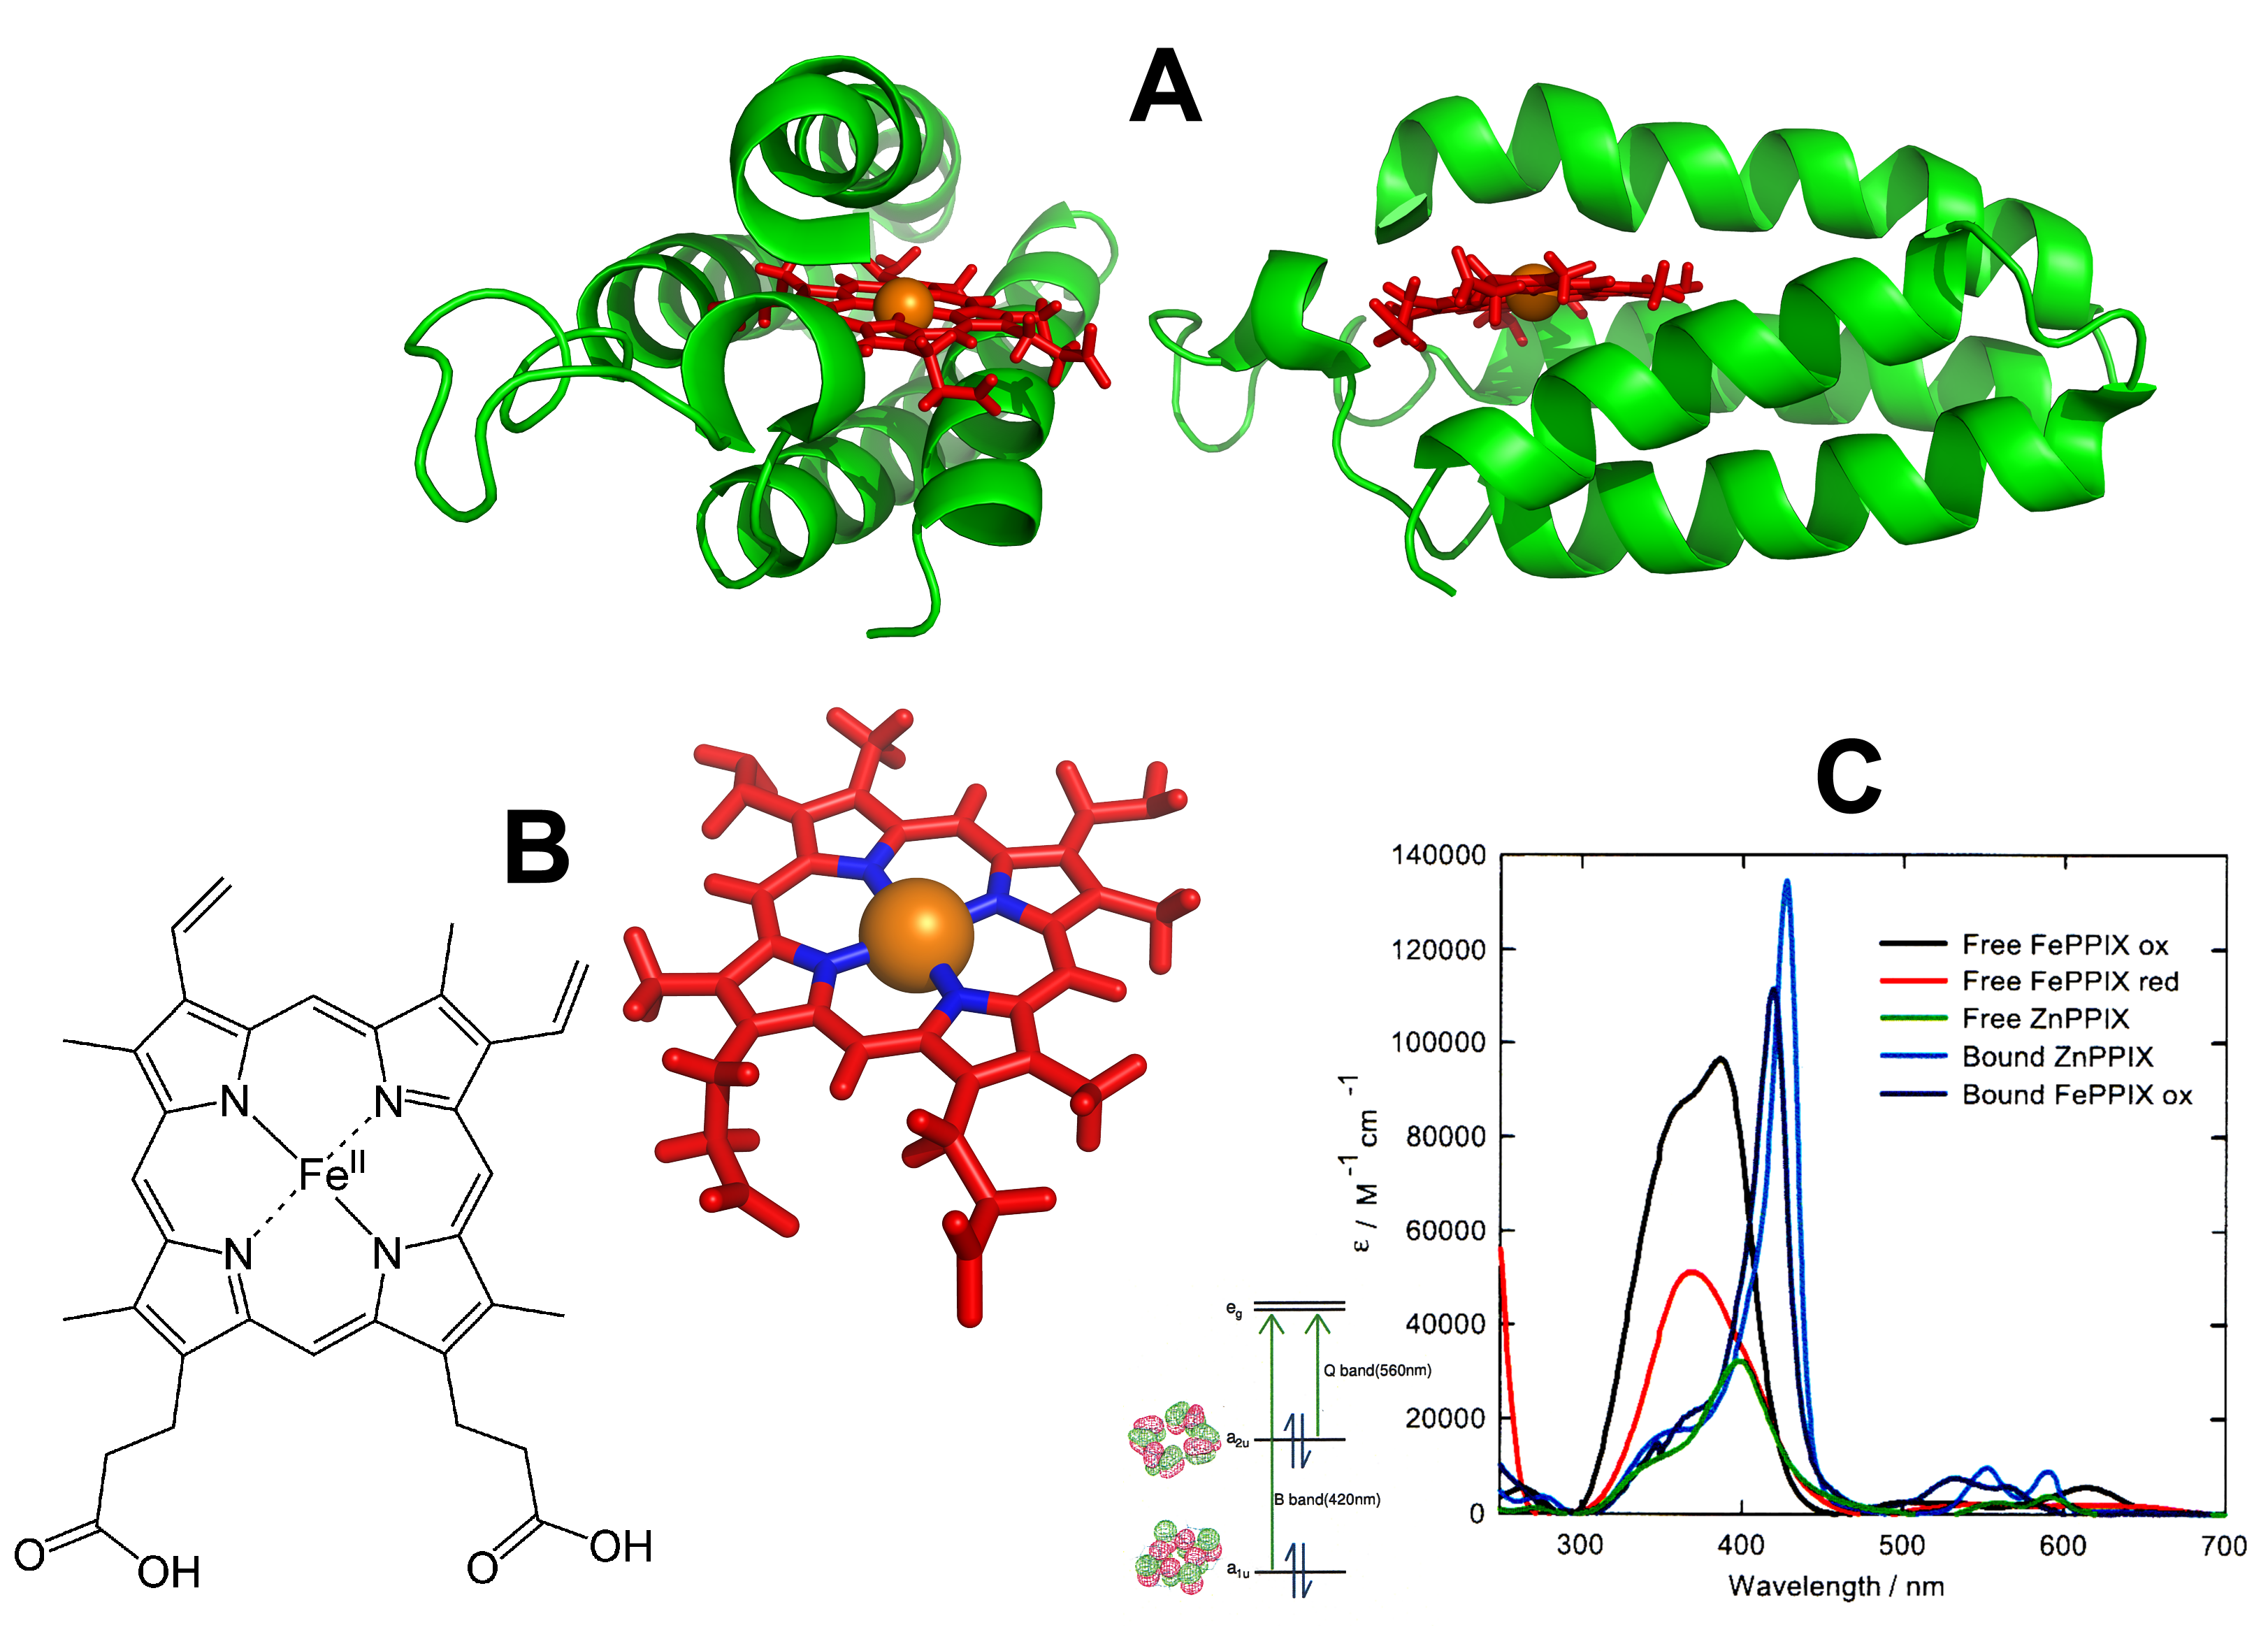
\includegraphics[width=137.4mm]{Images/haemStructure.png}
	\caption[Haem Structure]{A fancy image.}
	\label{fig:haemStructure}
\end{figure}
\end{verbatim}

\vspace{2ex}

\begin{figure}[!th]
	\centering
	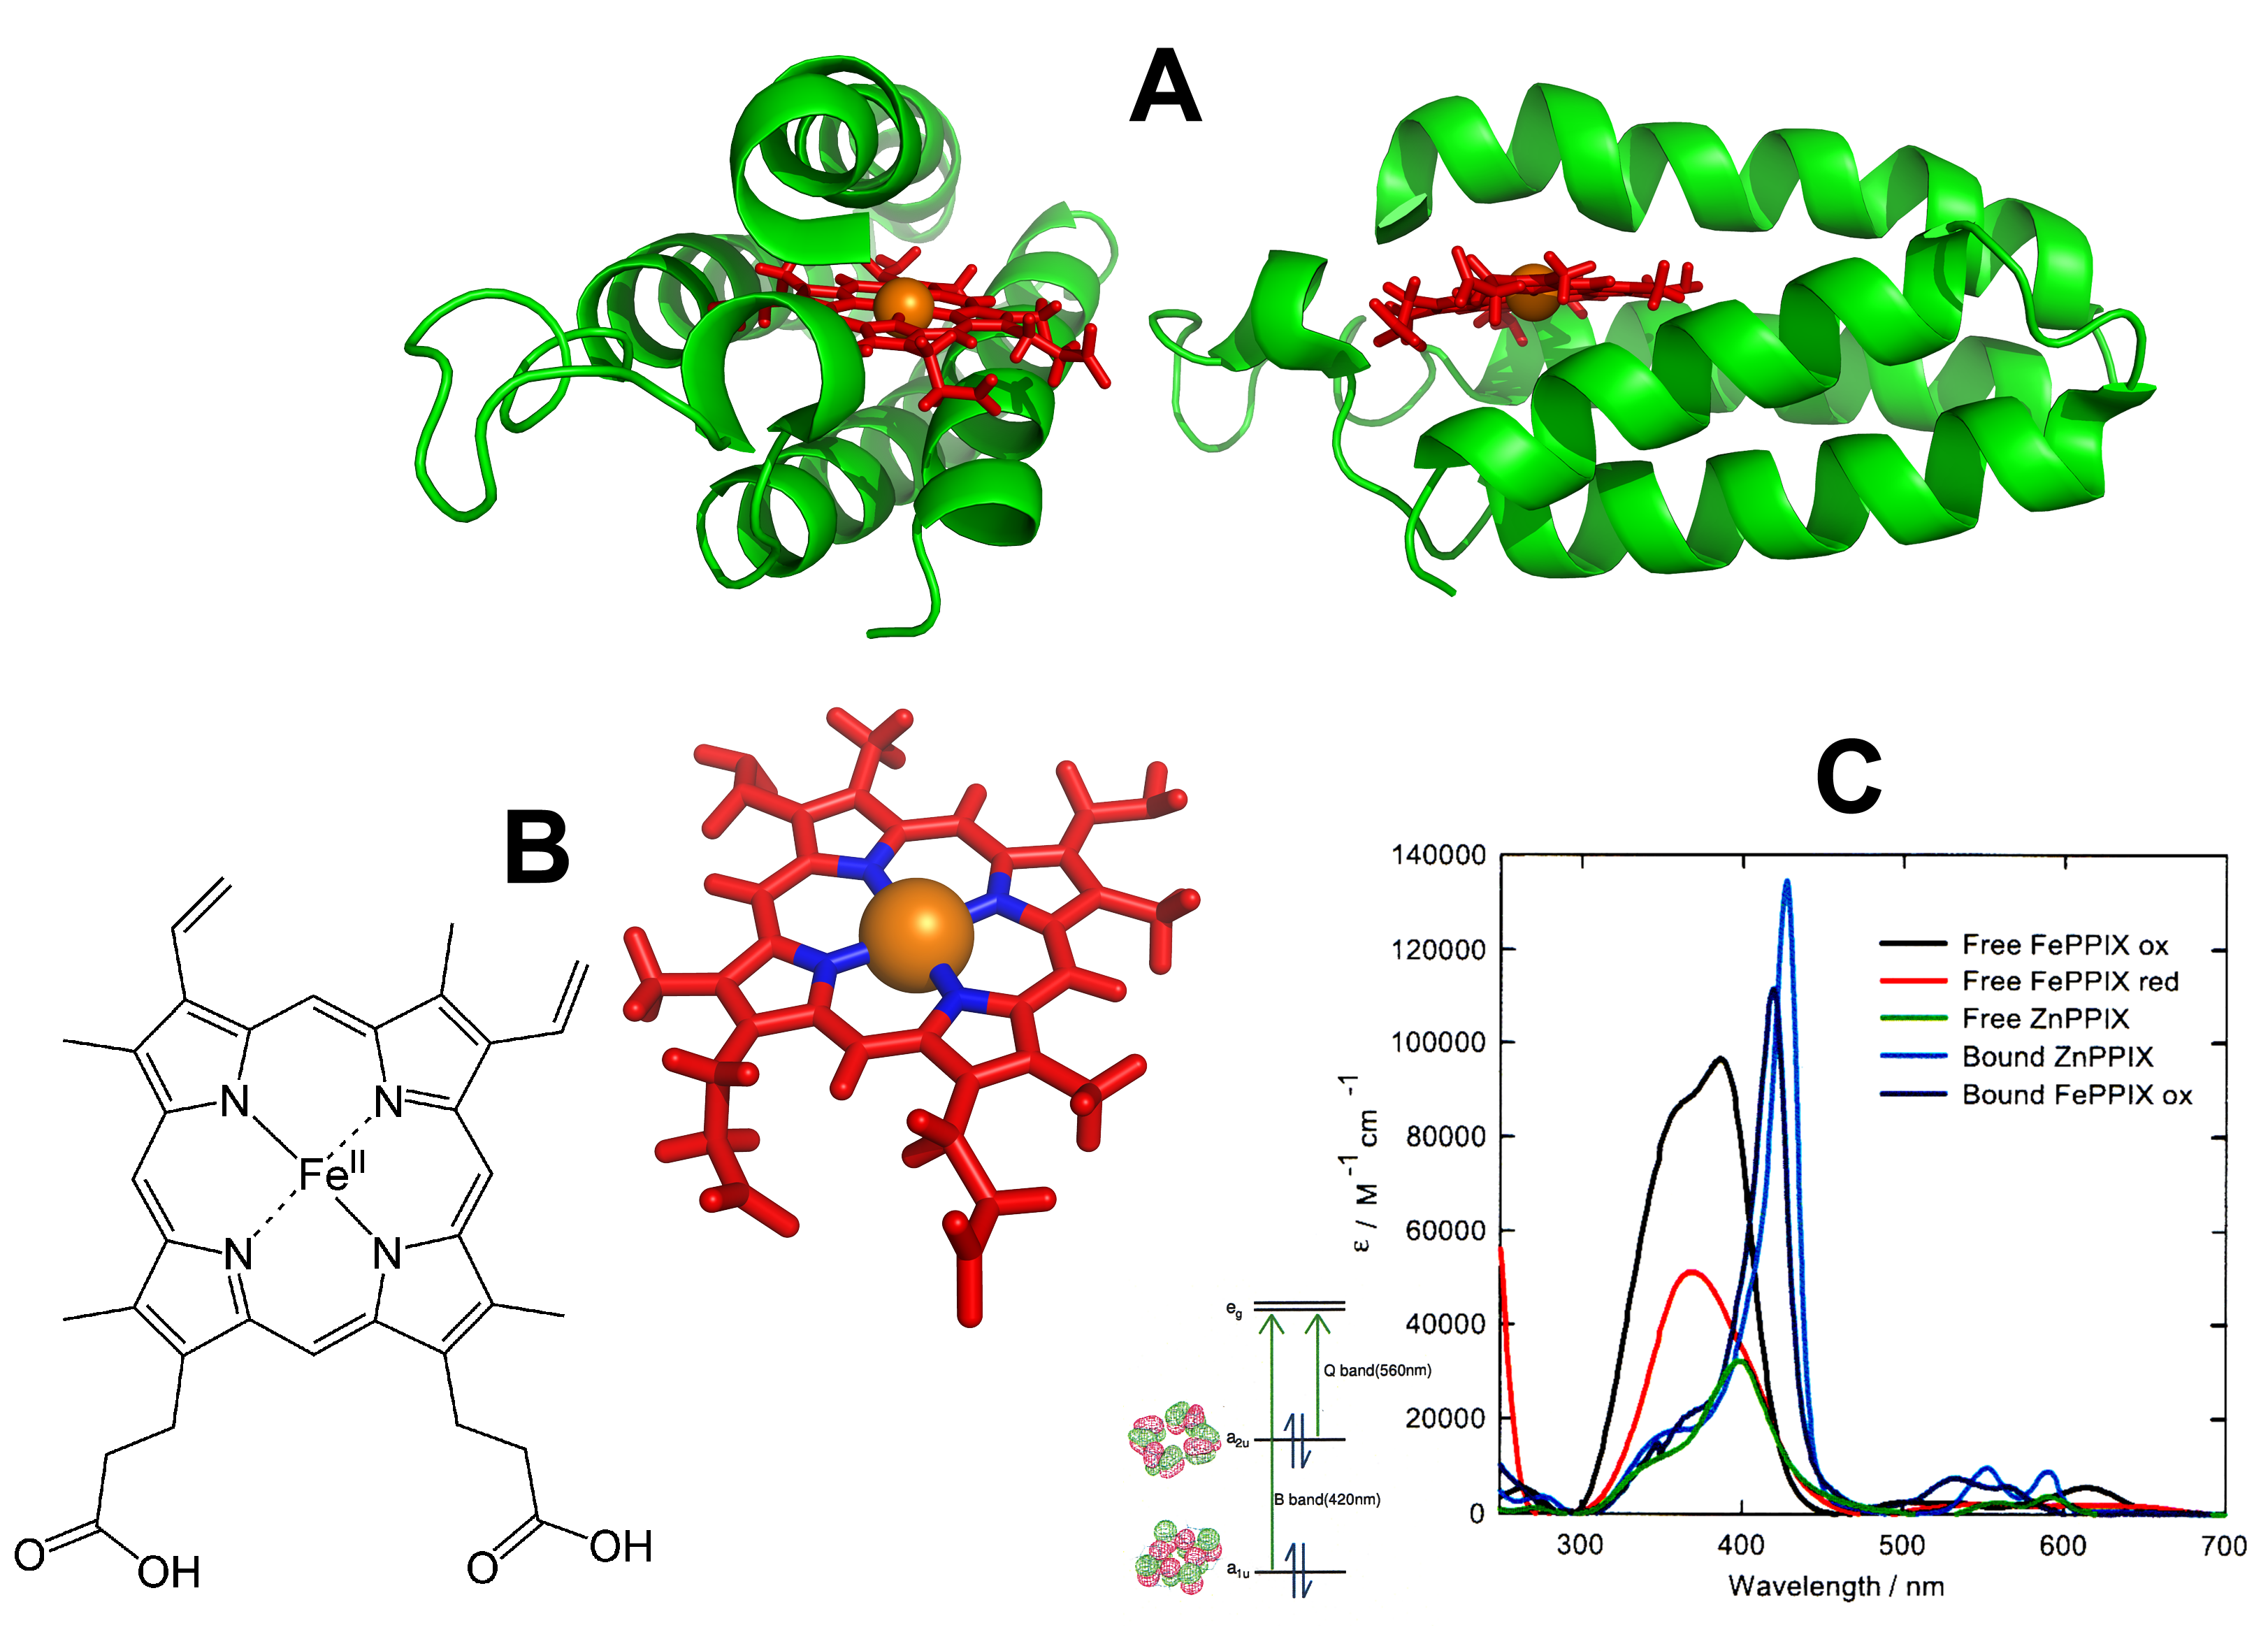
\includegraphics[width=137.4mm]{Images/haemStructure.png}
	\caption[Haem Structure]{A fancy image from Chris' Thesis.}
	\label{fig:haemStructure}
\end{figure}

In this example the command {\textbackslash}includegraphics tells LaTeX to look in the directory `Images' and incorporate the file called `haemStructure.png' into the final document while setting the width to 137.4mm.  This command can be used to resize a graphical file using the height or width parameter as shown. You must specify the units which can be pt, ex, em, mm, cm and so on. LaTeX recognises a very wide variety of standard units and graphics formats. The command is part of the graphicx package and so in the preamble you must include the command {\textbackslash}usepackage\{graphicx\}.

Many packages have been written to provide new commands. For example the `subfigure' package enables you to place separate images or files in the same figure side by side while giving them their own label. However, in this document we only concentrate on the very basics.

\section{Floating Environments}

Both tables and figures are examples of a `floating environments' which means LaTeX decides where to put them. 

The mysterious [!tbh] letters give guidance to LaTeX about roughly where the figure or table is  allowed to be, but in general they can move a long way from where you position them within your text file.  The letters in the square bracket can be t, h or b which stand for top, here or bottom.  If you don't specify any letters LaTeX defaults to [t].

LaTeX will always preserve the order in which figures appear.  If it cannot find a type setting solution, then it may move the float to it's own page, and combine it with other figures. If it still can't fit that in for some reason then it moves the float to the end of the document.  This has the effect of pushing all the remaining floating environments to the end of the document also.

The exclamation mark instructs LaTeX to ``try harder'' at putting the float where you told it to. Often you must play around to ensure the float positioning is acceptable, but usually this can be achieved by stretching or shrinking the image slightly using the size parameter, re-ordering text, judicial applications of the {\textbackslash}pagebreak command or by shouting loudly and slapping the computer monitor about. Note that it is better to resize the image using the original program that was used to create the image. Also using vector graphics can assist be useful (e.g. eps files) because they are designed to scale better.
\chapter{The Chapter on Making Chapters}
\label{sec:Chapters}

Right. LaTeX forces you to structure your document. There a series of simple commands for achieving this:

\vspace*{2ex}

{\textbackslash}chapter\{chapterName\}

{\textbackslash}section\{sectionName\}

{\textbackslash}subsection\{subsectionName\}

{\textbackslash}subsubsection\{subsubsectionName\}

\vspace*{2ex}

Easy enough. At the start of each chapter or section just issue one of these commands to name the section and LaTeX will present the chapter heading in the right style of font, which will be the same style of all the other heading names at that level of hierarchy throughout the document. In addition LaTeX assigns a number to that section. For example, this chapter was created using the command:

\vspace*{2ex}

{\textbackslash}chapter\{The Chapter on Making Chapters\} 

\vspace*{2ex}

LaTeX assigns the correct chapter number to each chapter in turn and then puts it in the table of contents, as you can see by looking at the table of contents! Easy.

\pagebreak
\section{The Section About Sections}
\label{sec:Section}
I think you're getting the hang of this. This section was created using the command {\textbackslash}section\{The Section About Sections\}. It appears in the table of contents as section \ref{sec:Section}.

\subsection{The Sub-Section About Sub-Sections}
\label{sec:SubSection}
Now you're really getting the hang of this. This subsection was created using the command {\textbackslash}subsection\{The Sub-Section About Sub-Sections\}. 

\subsubsection{The Sub-Sub-Section About Sub-Sub-Sections}
\label{sec:SubSubSection}
Now you're really getting the hang of this. but.. caught you out! This subsubsection doesn't have a number!  Ha Ha! It was created using the command {\textbackslash}subsubsection\{The Sub-Sub-Section About Sub-Sub-Sections\} in the same vein as all the other subsections/chapters etc. Here we have stopped the depth of the section numbering at the second level with the command:

\vspace*{2ex}

{\textbackslash}setcounter\{secnumdepth\}\{2\}

\vspace*{2ex}

Easy. WYSIWYM.  LaTeX does what you tell it to do. This is both a blessing and a curse.

\pagebreak
\section*{The Section About Sections That Don't Appear in the Table of Contents}
\label{sec:InvisibleSection}
Ok. Now we're throwing a spanner in the works. This section was created using the command:

\vspace*{2ex}

{\textbackslash}section*\{The Section About Sections That Don't Appear in the Table of Contents\}. 

\vspace*{2ex}

Notice how LaTeX has not assigned a number to the section and it doesn't appear in the table of contents. The effect of the * is to suppress the inclusion of a chapter, section or subsection in the automatic numbering. Easy. You can do this at any level. This is useful for things like prefaces, tables of contents or acknowledgements which you may or may not wish to have an entry in the main contents table. Up to you. It's your thesis. Don't just copy me.

\section{A Small Point About Numbering}

In this section notice how the numbering starts from where it left off before we suppressed the numbering on the previous section. Easy. WYSIWYM.
\pagebreak
\section{The Section About Internal Referencing}
\label{sec:InternalReferencing}

There are two related commands:

\vspace*{2ex}

{\textbackslash}label\{labelName\} 

{\textbackslash}ref\{labelName\}

\vspace*{2ex}


The {\textbackslash}label\{\} command allows you to create a label in a particular environment\footnote{That's right. Chapters, Sections and sub-sections etc are environments!}. The label won't appear in the final document. It's just a label which makes it easy to refer back to any particular environment elsewhere in the document. The {\textbackslash}ref\{\} command enables you to insert a reference anywhere in the document to any label in the document.  For example this is section \ref{sec:InternalReferencing}. The names you use in a label can be anything you like but musn't contain whitespace or special characters. I used the two commands:

\vspace*{2ex}

{\textbackslash}label\{sec:InternalReferencing\}

{\textbackslash}ref\{sec:InternalReferencing\}.

\vspace*{2ex}

The astute among you will realise that LaTeX has to read the document several times. Once to find the labels and then again to populate the references with the correct numbers. So you have to compile a latex document twice to get the referencing right. If there is a missing label or you refer to something that doesn't exist then latex inserts a convenient ? at that point. So hunting for queries is useful way of finding broken references. Latex issues warnings when it finds broken references.

As you create a document you will find yourself putting labels in all over the place so choose a sensible naming convention to help you remember the label names.

Each type of environment (equations, figures, tables, sections etc) has its own independent numbering system.  So when you choose your label name it's a good idea to have an identifier for that type of environment.  I have my own convention for label names which I use to help me remember references. E.g.   sec:SectionAboutCats. Eqn:EquationAboutCats,  Fig:FigureAboutCats and so on. This means you can differentiate between referring to the section or the figure more easily, even though they are about the same thing.

So Internal Referencing is a doddle. Easy!
\chapter{External Referencing}

Referencing is usually performed using a separate program called BibTex.  This program understands the file format .bib.

To create a reference within your document first you must create a .bib file by exporting your list of references from which ever referencing software you used, such as endnote, mendeley or whatever you use.

You can refer to an entry in the .bib file using the {\textbackslash}cite\{ref:Name\} command. the identifier `ref:Name' is the unique identifier which is the first line of each item included in your bibliography file.

For example, open the file LaTexCourseBib.bib in the bibliography directory. The first entry has the identifier `Horcas2007'.  This can be invoked as follows:


\begin{verbatim}
For example, this interesting fact\cite{Horcas2007}, is a cracking example.
\end{verbatim}

For example, this interesting fact\cite{Horcas2007}, is a cracking example.

During compilation latex and bibtex co-operate. During the first compilation latex generates a list of references that it needs.  During the second compilation bibtex populates the details from the .bib file into a shorter, ordered .bib file. The third compilation inserts markers at the right place in the main file and the fourth compilation generates the final list of references. Thus the compilation sequence is latex, bibtex, latex, latex.

The style of the referencing format can be changed using the command {\textbackslash}bibliographyStyle\{\}. e.g. the style used in this document is cjfthesisv1.bst which is invoked by 

\begin{verbatim}
\bibliographystyle{Bibliography/cjfthesisv1}
\end{verbatim}

The location of the list of references in the document is specified by issuing the {\textbackslash}bibliography\{\} command which also specifies the master bibliography file.

\begin{verbatim}
\bibliography{Bibliography/LaTeXCourseBib}
\end{verbatim}




\chapter{Organising Your Files}
One of the drawbacks of word is that the figures and tables are included within the document which becomes very very clunky quite quickly and once it reaches around 100Mb it becomes unwieldy and hard to export. One of that advantages of LaTeX is that the files are all text files and so are very light on resources and are easy to email around the place.

However, sometimes it can be difficult to navigate through a single text file, so if you had a huge document then it becomes difficult to find your way around.  One way of circumnavigating this problem is to break the file up into smaller files. As long as LaTeX knows where to look you can have a file for each logical sub-division of your document.

Therefore it is worth spending a bit of time at the beginning of a large project deciding how you wish to break up your LaTex Files and organise them neatly and tidily.  You can then tell LaTex where to look for the files using the following command:

\vspace*{2ex}
{\textbackslash}include\{fileName\}
\vspace*{2ex}

\pagebreak
\section{Linking a File}
We are now going to copy part of the tutorial file into a separate files and link it the main file.  Because this could go wrong it is sensible to back up tutorial.tex as something else. So save a copy called `tutorialOriginal.tex' for safe keeping. Then follow the following instructions.

\begin{enumerate}
\item Create a new file called MyFirstPage.tex
\item Select and Cut out the first chapter of Tutorial.Tex
\item Paste the first chapter into MyFirstPage.tex
\item Save both tutorial.tex and MyFirstPage.tex
\item Then add {\textbackslash}include\{MyFirstPage\} in tutorial.tex where the text used to be before you cut it out. We don't need to add the `.tex' because LaTeX can only include `.tex' files.
\item compile tutorial.tex and view the PDF
\end{enumerate}

The final PDF should look exactly the same as it was! except we now have a separate file for one of the chapters.

\pagebreak
\section{Creating A Class File}
We can also save our preamble in a separate file called a class file. This makes your main document much easier to understand.  To make it work we need to use the {\textbackslash}LoadClass\{\} command as follows: 

\begin{enumerate}
\item Create another new file and save it as TutorialStyle.cls
\item Copy the preamble of tutorial.tex into the new file. Starting with the {\textbackslash}documentclass{} command and copy right up to, but not including, the {\textbackslash}begin{document} command. Delete the preamble in the original document.
\item Save TutorialStyle.cls and tutorial.tex
\item Modify the first line of TutorialStyle.cls by replacing the word `document' with the word `Load'.
\item Add a new first line of tutorial.tex to use your new style class {\textbackslash}documentclass\{TutorialStyle\}
\item Save both files.
\end{enumerate}

\subsection{Sanity Check}

The first line of TutorialStyle.cls should now be:

\begin{verbatim}
\LoadClass[12pt, oneside, a4paper]{book}
\end{verbatim}
\vspace{2ex}

The first line of tutorial.tex should be:

\begin{verbatim}
\documentClass{TutorialStyle}
\end{verbatim}
\vspace{2ex}

We have just created what is called a style file. You can use this style file as a generic preamble for other documents as well. Compile tutorial.tex.  Nothing should have changed in the final PDF.


\pagebreak
\section{The Structure of this Document}

Lets now look at how I've organised this document. It is identical to my thesis because it started out life as my thesis. I usurped the structure and simply replaced the headings and content to make a kind of reference manual for this introductory course. This document therefore is three things:

\begin{enumerate}
\item An example thesis structure to work from.
\item The LaTeX files which were used to create it can be used as a template for a thesis.
\item It is also a convenient introductory latex manual!
\end{enumerate}

\vspace*{2ex}
Groovy huh?

\section{The Master File}

There is a master file where LaTeX begins the compilation procedure. This contains the {\textbackslash}documentclass command needed to set the ball rolling. Within the file there are a series of {\textbackslash}include\{\} commands, one for each Chapter, which tell LaTeX where to find the files containing each chapter.

The subfiles cannot be compiled on their own because they do not contain the {\textbackslash}documentclass, {\textbackslash}begin\{document\} or {\textbackslash}end\{document\} commands. Lets us look in more detail at the master file and we will learn some new LaTeX commands.

\singlespacing
\pagebreak
\begin{verbatim}
\documentclass{Style/LatexCourseStyle}

\begin{document}
\setcounter{secnumdepth}{2}
\setcounter{tocdepth}{1}

\frontmatter
\onehalfspacing
\include{Frontmatter/Titlepage}
\include{Frontmatter/Declaration}
\include{Frontmatter/Acknowledgements}
\include{Frontmatter/Summary}
\include{Frontmatter/Abbreviations}
\tableofcontents
\listoftables
\listoffigures

\mainmatter
\renewcommand{\sectionmark}[1]{\markright{\thesection \ #1}{}}
\include{Chapters/Overview}
\include{Chapters/MyFirstPage}
\include{Chapters/Lists}
\include{Chapters/mathsEquations}
\include{Chapters/ChemicalEquations}
\include{Chapters/Tables}
\include{Chapters/Figures}
\include{Chapters/Sectioning}
\include{Chapters/externalReferencing}
\include{Chapters/ThesisTemplateMainFile}
%\include{Chapters/ChapterThatIsNotCompiled}

\appendix
%\include{Appendices/UsefulWebsites}

\singlespacing

\backmatter
\addcontentsline{toc}{chapter}{References}
\bibliographystyle{Bibliography/cjfthesisv1}
\renewcommand{\bibname}{References}
\bibliography{Bibliography/LatexCourseBib}

\end{document}
\end{verbatim}
\onehalfspacing
\pagebreak

\section{Analysing the Master File}
Let us go through this file and observe the new commands. Most of it is self-explanatory.

\begin{verbatim}
\documentclass{Style/LaTeXCourseStyle}
\end{verbatim}

This command tells latex that the document class is the one defined in the the style file ''LaTeXCourseStyle'', which is in the sub directory ''style''.  Easy.

\begin{verbatim}
\setcounter{secnumdepth}{2}
\setcounter{tocdepth}{1}
\end{verbatim}

The first of these commands tells latex that the section depth number is 2. I.E. throughout the document only bother numbering sections, subsections and subsubsections down to the second level (such as section 1.2.3). The second command tells latex to only build the table of contents from section numbers down to the first level i.e. 1.1.  Easy enough.

The command {\textbackslash}frontmatter is exclusive to the book class, on which this style is based, and tells latex that within this section to number the pages using roman numerals, and not to include these numbers in the table of contents, just like in a book. The {\textbackslash}mainmatter and {\textbackslash}backmatter commands similarly delineate the other sections of the document.  

Childs play.  How long would it take you to figure out how to do that in word???? No idea. I've never tried.

Note that these rather cool commands are not available in every single class. So for a paper you would use the article class where such compartmentalisation of your document is not appropriate. In fact you can often download latex templates from the journal to wish to submit your paper, which is why I concentrate on the thesis template in this course.

\begin{verbatim}
\onehalfspacing
\end{verbatim}

Is obvious. ''From this point forward use line spacing of one and a half lines please. Thank you.'' How many hours have you spent clicking on paragraph indentations for each separate paragraphs in word? Nightmare. Want to change the standard in the whole document? Not a chance in word. In latex, you can do it with a single word, carefully placed in the master file.

\begin{verbatim}
\include{Frontmatter/Titlepage}
\include{Frontmatter/Declaration}
\include{Frontmatter/Acknowledgements}
\include{Frontmatter/Summary}
\include{Frontmatter/Abbreviations}
\end{verbatim}

The {\textbackslash}include\{\} command tells latex to include the specified .tex file at this point.  Thus it is a simple matter to break up a large document into sub components.  I have written each part of the front matter in a separate file and then grouped all the front matter into one directory called: Frontmatter.

See how the directory structure of my files reflects the structure of my book?

\begin{verbatim}
\tableofcontents
\listoftables
\listoffigures
\end{verbatim}

Again. This is easy. These commands mean: ''Please scan through the whole document and build for me a table of contents, a list of tables, a list of figures and then write down the entries along side their section numbers (as I have them ordered in this version of the document), as well as the page numbers on which they appear and create a nice little summary table and add them to the front matter of my document. Thanks.''.

How does latex do this?  remember the idea of environments?  Well each table, figure, equation etc is a defined environment.  LaTeX just counts them up and assigns numbers starting wherever you want and builds a table.  You can tell latex to ignore individual sections if you want to.

You can also control the look and feel of your table of contents with subtley and grace. Do you want to fill the white space with lines of dots to aid readability, even though the chapter titles are all different lengths? page numbers? How deep should the TOC been?  etc etc etc. How to do this is beyond the scope of this course, but now you know about it, go look it up. easy as $\pi$.

Ok.

Main matter we've done.

\begin{verbatim}
\renewcommand{\sectionmark}[1]{\markright{\thesection \ #1}{}}
\end{verbatim}

This command tells latex to 'renewcommand', i.e. change the meaning of the following command from this point in the document forward, over-riding previous definitions.
\begin{verbatim}
\sectionmark}[1]{\markright{\thesection \ #1}{}
\end{verbatim}

Is latex speak for ``please write the section heading at the top right hand side of each page. thanks''. This works in conjunction with a command in the style file which we'll talk about later. You have to tell latex to switch on headings as well as where to put them.

\begin{verbatim}
\include{Chapters/Overview}
\include{Chapters/MyFirstPage}
\include{Chapters/Lists}
\include{Chapters/mathsEquations}
\include{Chapters/ChemicalEquations}
\include{Chapters/Tables}
\include{Chapters/Figures}
\include{Chapters/Sectioning}
\include{Chapters/externalReferencing}
\include{Chapters/ThesisTemplateMainFile}
%\include{Chapters/ChapterThatIsNotCompiled}
\end{verbatim}

This is the include command again. You will notice that one of the include lines is commented out. This is a handy trick to only build certain parts of my thesis. Which can be useful if individual chapters are being reviewed.

\pagebreak

\begin{verbatim}
\appendix
%\include{Appendices/UsefulWebsites}

\singlespacing

\backmatter
\addcontentsline{toc}{chapter}{References}
\bibliographystyle{Bibliography/cjfthesisv1}
\renewcommand{\bibname}{References}
\bibliography{Bibliography/LatexCourseBib}
\end{verbatim}

The rest is easy. {\textbackslash}Appendix means we are in the appendix now and start labelling sections with A.1.2 instead of 1.2.3.  

{\textbackslash}addcontentsline means forcibly insert a contents line about the references into the contents table. 

{\textbackslash}\{bibliographystyle\{Bibliography/cjfthesisv1\}\} means use the biblography style defined in the file cjfthesisv1. Defining a bibliography style will be covered later if we have time. This is where you specify how the references will appear (names, journals, full stops, commas etc).

{\textbackslash}renewcommand\{{\textbackslash}bibname\}\{References\} means: rename the bibliography chapter as `References'

{\textbackslash}biblography means add the following bibliography.  You can reference entries in this bibliography file very easily.

The astute among you will realise that LaTeX will have to read the document several times before it can be compiled with all the references.  Hey ho. No problem. You can go and have a cuppa while LaTeX does your references for you in the style of your favorite journal... nice.




%\include{Chapters/ChapterThatIsNotCompiled}
\end{verbatim}

This is the include command again. You will notice that one of the include lines is commented out. This is a handy trick to only build certain parts of my thesis. Which can be useful if individual chapters are being reviewed.

\pagebreak

\begin{verbatim}
\appendix
%\include{Appendices/UsefulWebsites}

\singlespacing

\backmatter
\addcontentsline{toc}{chapter}{References}
\bibliographystyle{Bibliography/cjfthesisv1}
\renewcommand{\bibname}{References}
\bibliography{Bibliography/LatexCourseBib}
\end{verbatim}

The rest is easy. {\textbackslash}Appendix means we are in the appendix now and start labelling sections with A.1.2 instead of 1.2.3.  

{\textbackslash}addcontentsline means forcibly insert a contents line about the references into the contents table. 

{\textbackslash}\{bibliographystyle\{Bibliography/cjfthesisv1\}\} means use the biblography style defined in the file cjfthesisv1. Defining a bibliography style will be covered later if we have time. This is where you specify how the references will appear (names, journals, full stops, commas etc).

{\textbackslash}renewcommand\{{\textbackslash}bibname\}\{References\} means: rename the bibliography chapter as `References'

{\textbackslash}biblography means add the following bibliography.  You can reference entries in this bibliography file very easily.

The astute among you will realise that LaTeX will have to read the document several times before it can be compiled with all the references.  Hey ho. No problem. You can go and have a cuppa while LaTeX does your references for you in the style of your favorite journal... nice.




%\include{Chapters/ChapterThatIsNotCompiled}

\appendix
%\include{Appendices/UsefulWebsites}

\singlespacing

\backmatter
\addcontentsline{toc}{chapter}{References}
\bibliographystyle{Bibliography/cjfthesisv1}
\renewcommand{\bibname}{References}
\bibliography{Bibliography/LatexCourseBib}

\end{document}
\end{verbatim}
\onehalfspacing
\pagebreak

\section{Analysing the Master File}
Let us go through this file and observe the new commands. Most of it is self-explanatory.

\begin{verbatim}
\documentclass{Style/LaTeXCourseStyle}
\end{verbatim}

This command tells latex that the document class is the one defined in the the style file ''LaTeXCourseStyle'', which is in the sub directory ''style''.  Easy.

\begin{verbatim}
\setcounter{secnumdepth}{2}
\setcounter{tocdepth}{1}
\end{verbatim}

The first of these commands tells latex that the section depth number is 2. I.E. throughout the document only bother numbering sections, subsections and subsubsections down to the second level (such as section 1.2.3). The second command tells latex to only build the table of contents from section numbers down to the first level i.e. 1.1.  Easy enough.

The command {\textbackslash}frontmatter is exclusive to the book class, on which this style is based, and tells latex that within this section to number the pages using roman numerals, and not to include these numbers in the table of contents, just like in a book. The {\textbackslash}mainmatter and {\textbackslash}backmatter commands similarly delineate the other sections of the document.  

Childs play.  How long would it take you to figure out how to do that in word???? No idea. I've never tried.

Note that these rather cool commands are not available in every single class. So for a paper you would use the article class where such compartmentalisation of your document is not appropriate. In fact you can often download latex templates from the journal to wish to submit your paper, which is why I concentrate on the thesis template in this course.

\begin{verbatim}
\onehalfspacing
\end{verbatim}

Is obvious. ''From this point forward use line spacing of one and a half lines please. Thank you.'' How many hours have you spent clicking on paragraph indentations for each separate paragraphs in word? Nightmare. Want to change the standard in the whole document? Not a chance in word. In latex, you can do it with a single word, carefully placed in the master file.

\begin{verbatim}
\thispagestyle{empty}

\begin{center}
\vspace*{\stretch{1}}

\hrule height 2pt
\vspace*{2ex}
{\Huge\textbf{Towards the Ability to Make Super Duper LaTeX Documents}\par}
\vspace*{2ex}
\hrule height 2pt
\vspace*{10ex}
{
\includegraphics[height=40mm]{Images/UnivShield}\par}
\vspace*{10ex}
{\large\textbf{Christopher~James~Forman}\par}
\vspace*{2ex}
{\large{Department Of Chemistry}\par}
\vspace*{2ex}
{\large{University of Cambridge}\par}
\vspace*{5ex}
{\large{This dissertation is submitted for the degree of \textit{Doctor of Philosophy}}\par}
\vspace*{5ex}
{\large{\today}\par}

\vspace*{\stretch{2}}
\end{center}
\chapter*{Declaration}

\vfill

This dissertation is the result of my own work and includes nothing which is the outcome of work done in collaboration except where specifically indicated in the text. It is not substantially the same as any that I have submitted for a degree or diploma or other qualification at any other University and no part has already been, or is concurrently being, submitted for any degree, diploma, or other qualification. It does not exceed 60,000 words, including tables, footnotes, bibliography and appendices.\par

\vspace{10ex}

\begin{flushright}
Signature: \rule[0pt]{60mm}{0.5pt}

\vspace{5ex}

Date: \rule[0pt]{60mm}{0.5pt}
\end{flushright}

\vfill
\chapter*{Acknowledgments}
\subsection*{Family}
Mum. Dad. Pet Dog.

\subsection*{Scientific Collaborations}
Dr A.N.Other at uni of blah for samples and instrument time etc. My Amazing Lab Chums.

\subsection*{Scientific Support}
My amazing lab chums.

\subsection*{General Assistance}
Cleaner, My amazing lab chums.

\subsection*{Financial Support}
Bank, Tax payer. My amazing lab chums.

\subsection*{Moral Support}
My Amazing Lab chums.

\subsection*{Academic Inspiration}
Netwon, My super. My Amazing Lab Chums.

\subsection*{Everyone else}
My Amazing Lab Chums.

\chapter*{Summary}
This document is a handbook for introducing you to LaTeX. It contains a bit of background about the history and philosophy of LaTeX.  However, it concentrates on providing a guided practical introduction to the basic techniques such as 
\begin{itemize}
\item Lists
\item Mathematical and chemical equations
\item Tables
\item Figures
\item Chapters and Sections
\item Linking to other files in large documents
\item Referencing
\end{itemize}

The handbook is also presented in the style of a thesis. This means that source files provided on the introductory course and available from the department web page are a convenient template for a thesis.

More details on specific aspects of LaTeX can be found at the departmental LaTeX page which can be found here:

 http://www-ch-int.ch.private.cam.ac.uk/latex/about

\chapter*{Abbreviations}

\begin{longtable}{r >{\rule{0pt}{3ex}}l<{\rule[-1.5ex]{0pt}{0pt}}}
ADP & Adenosine Diphosphate\\
(nc/c)AFM & (non-contact/conducting) Atomic Force Microscopy\\
ATP & Adenosine Triphosphate \\
\end{longtable}
\end{verbatim}

The {\textbackslash}include\{\} command tells latex to include the specified .tex file at this point.  Thus it is a simple matter to break up a large document into sub components.  I have written each part of the front matter in a separate file and then grouped all the front matter into one directory called: Frontmatter.

See how the directory structure of my files reflects the structure of my book?

\begin{verbatim}
\tableofcontents
\listoftables
\listoffigures
\end{verbatim}

Again. This is easy. These commands mean: ''Please scan through the whole document and build for me a table of contents, a list of tables, a list of figures and then write down the entries along side their section numbers (as I have them ordered in this version of the document), as well as the page numbers on which they appear and create a nice little summary table and add them to the front matter of my document. Thanks.''.

How does latex do this?  remember the idea of environments?  Well each table, figure, equation etc is a defined environment.  LaTeX just counts them up and assigns numbers starting wherever you want and builds a table.  You can tell latex to ignore individual sections if you want to.

You can also control the look and feel of your table of contents with subtley and grace. Do you want to fill the white space with lines of dots to aid readability, even though the chapter titles are all different lengths? page numbers? How deep should the TOC been?  etc etc etc. How to do this is beyond the scope of this course, but now you know about it, go look it up. easy as $\pi$.

Ok.

Main matter we've done.

\begin{verbatim}
\renewcommand{\sectionmark}[1]{\markright{\thesection \ #1}{}}
\end{verbatim}

This command tells latex to 'renewcommand', i.e. change the meaning of the following command from this point in the document forward, over-riding previous definitions.
\begin{verbatim}
\sectionmark}[1]{\markright{\thesection \ #1}{}
\end{verbatim}

Is latex speak for ``please write the section heading at the top right hand side of each page. thanks''. This works in conjunction with a command in the style file which we'll talk about later. You have to tell latex to switch on headings as well as where to put them.

\begin{verbatim}
\chapter{Overview}
\label{chap:overview}
\section{LaTeX: The answer to everything.}
LaTeX is typsetting program that takes an input file of marked up text and then, with a user defined set of rules, typesets a beautifully crafted output file that can be easily printed (e.g. a pdf). 

\subsection{Advantages}

The advantages of this method are manifold:

\begin{itemize}

\item Use any text editor to view the source document.
\item More time can be spent working on the content and not worrying about how text or figures interact in the layout until later on.
\item LaTeX uses consistent rules throughout a document
\item LaTeX sorts out basic typesetting automatically
\item Changes can be introduced globally with very little effort
\item Document structure is explicit
\item Documents can be professionally typeset and look great
\item You are forced to structure your documents correctly.
\item Mathematical equations, like $E=mc^2$ or $\imath\hbar\frac{\partial}{\partial t}\Phi (x, t) = \hat{H}\Phi (x, t)$ can be produced almost as fast as typing (if you know the commands!).
\end{itemize}

\subsection{Disadvantages}
The disadvanatges of this method are also manifold:
\begin{itemize}
\item You don't see the output as you go.
\item Steep learning curve.
\item Documents are harder to edit by a second author (unless they are adept at LaTeX too). This can be mitigated using version control, which makes group authoring processes superior to word.
\item The program never works quite the way you want it to and learning how to influence it can be problematic and subtle.
\item Although intended to save work the principle of 'conservation of work' means that you simply transform problems associated with WYSISYG approaches to problems associated with WYSIWYM approaches!
\item You can go blind trying to determine the difference between wiggly and smooth brackets if your editors font isn't large enough.
\end{itemize}

\subsection{On balance?}
If it's so rubbish, why use LaTeX?

\begin{itemize}
\item Large documents are much more easily handled. 
\item In general it is quicker to debug a LaTeX document than typeset an entire thesis manually. 
\item Technical information such as tables, equations and figures are integrated much more smoothly than with word.
\end{itemize}

\section{How does it work?}

The raw text is interspersed with commands, preceded by a \textbackslash, which tell LaTeX what to do with the text. For example you can \textbf{make it bold}, \emph{italic}, or \underline{underlined} with the commands {\textbackslash}textbf\{\}, {\textbackslash}emph\{\} or {\textbackslash}underlined\{\}. More on commands in a moment...



\chapter{My First Page}

\section{The Very Beginning}
The very simplest LaTeX document might look like this:

\begin{verbatim}
\documentclass[a4paper,12pt]{article}
\begin{document}
Hello World.
\end{document}
\end{verbatim}

\pagebreak
\thispagestyle{empty}
Hello World.
\pagebreak
\subsection{Break Down}
What's all the gobbledegook around my simple message???

In LaTeX we intersperse text and commands.  Commands are preceded by a \textbackslash. For example the first line in a LaTeX document \underline{\textbf{\emph{must}}} be:

\begin{verbatim}
\documentclass[options]{class}
\end{verbatim}

Where the word ''class'' may be substituted for one of many things such as: article, proc, minimal, report, book, letter, memoir, slides, beamer.

Similarly, and completely generally in LaTeX speak, the square brackets denote the existence of optional parameters. Each individual command can take its own parameters and for the ''{\textbackslash}documentclass'' command there are options for controlling font size, font family, landscape, oneside, twosided, page size and so on. These options will persist throughout the entire document. For example the document class command for this document, (which is likely to be like the one you would use for a thesis), would be:

\begin{verbatim}
\documentclass[12pt, oneside, a4paper]{book}
\end{verbatim}

Other options include:

\begin{itemize}
\item {10pt, 11pt, 12pt (default is 10pt).}
\item {letterpaper, legalpaper, a4paper, executivepaper, a5paper, b5paper}
\end{itemize}
and so on.

\pagebreak
\section{Can I start typing please?}

After we have set up the document we can start actual work on our document. So we must tell LaTeX that what follows is to be interpreted as a document.  The command {\textbackslash}begin can take many different parameters and is a command to enter what is known, in LaTeX speak, as 'an environment'. Thus the commands:
\begin{verbatim}
\begin{document}

\end{document}
\end{verbatim}

tells LaTeX to enter and leave the document environment, and thus constitute the outer limits of our document file. Other environments include the equation environment, the itemize environment, the figure environment and so on. These will be encountered in due course.

Every part of the LaTeX file is therefore within an environment of specific type and the content within each environment consists of commands or text.

That's basically it.

So let's get on with it shall we...

\pagebreak
\section{The ground rules}
\begin{quote}
Hold on, hold on, hold on my son.

First the lessons.

Then the fun!
\end{quote}
Dr Seuss.

\subsection{Spaces}
Whitespace characters, such as blank or tab, are treated uniformly as space by LaTeX. Several consecutive whitespace characters are treated as one single space. Whitespace at the start of a line is generally ignored, and a single line break is treated as whitespace. An empty line between two lines of text defines the end of a paragraph. Several empty lines are treated the same as one empty line. The text below is an example.

\begin{verbatim}
It does not matter whether you
enter one or several             spaces
after a word. The final result will be typeset beautifully
according    to     precise rules.




An empty line starts a new
paragraph. Note the indentation on the first line of the paragraph, 
except at the beginning of the section. 
\end{verbatim}

\vspace*{2ex}
\vspace*{2ex}

It does not matter whether you
enter one or several             spaces
after a word. The final result will be typeset beautifully
according    to     specific rules.




An empty line starts a new
paragraph. Note the indentation on the first line of the paragraph, except at the beginning of the section. 

\pagebreak
\subsection{Special Characters}
The symbols 

\# \$ \% \textasciicircum{} \& \_ \{ \} \~{} \textbackslash

are reserved characters that either have a special meaning under LaTeX or are unavailable in all the fonts. If you enter them directly in your text, they will normally not print, but rather make LaTeX do strange things.

To overide the special meanings of these symbols and allow them to produced within your text you may use the following sequences:
\begin{verbatim}
\# \$ \% \textasciicircum{} \& \_ \{ \} \~{} \textbackslash
\end{verbatim}

Other symbols and many more can be printed with special commands in mathematical formulae or as accents.

The backslash character '\textbackslash' cannot be entered by adding another backslash in front of it ( \textbackslash\textbackslash); because this sequence means ''linebreak''.

The command \textbackslash\~{}\{\} produces a tilde which is placed over the next letter. For example \textbackslash\~{}\{n\} gives \~{n}. To produce just the character \~{}, use \textbackslash\~{}\{\} which places a \~{} over an empty box.

Similarly, the command \textbackslash\textasciicircum{} produces a hat over the next character, for example \textbackslash\textasciicircum\{o\} produces \^{o}.

\pagebreak
\section{Preamble}
After the {\textbackslash}documentclass command we add ''preamble''. Here we load special features that we will use throughout our document to expand on the basic capabilities of LaTex. These are contained in units called ''packages'' which we can tell our LaTeX compiler to download by using the command ''{\textbackslash}include\{packageName\}''. 

There are many repositories of such packages on the web. Your compiler generally knows where to look and most standard packages are included with any install. For example, to include a special set of typesetting instructions to handle chemical equations we can grow our simple document with a single command like this:

\begin{verbatim}
\documentclass[a4paper,12pt]{article}
\usepackage[version=3]{mhchem}
\begin{document}
Hello World!

We all need \ce{H2O}.

I'm less fussed about \ce{^{235}_{92}U+}.

\end{document}
\end{verbatim}

\vspace{2ex}

\pagebreak
\thispagestyle{empty}
Hello World!

We all need \ce{H2O}.

I'm less fussed about \ce{^{235}_{92}U+}.
\pagebreak

Here we have loaded a package called: "`mhchem"' which took the option ''[version=3]''. This is a package for drawing chemical equations easily and it has it's own instruction manual which you can follow easily. It is included in the bundle of files for this course.

Other things we can do in the premable within LaTeX are to redefine existing commands or create our own personal commands. These can be stored in a file called the 'style file' which we can load at the beginning of our document, in place of our documentclass. More about this later on...


\subsection{Comments}
It is often useful to comment your LaTeX documents. You can leave yourself amusing, sarcastic messages that won't get printed out in the final document. Use this to make your own notes as the course progresses.

To get a comment use the \% command, which tells LaTeX to ignore the rest of the line, the line break and all the white space at the beginning of the next line, for example, we may add to our continually evolving document...

\begin{verbatim}
\documentclass[a4paper,12pt]{article}
\usepackage[version=3]{mhchem}
\begin{document}
Hello World!

%All humans need water and I would like 
%to include this concept in my arguments.
We all need \ce{H2O}.

%Uranium 235 is toxic, which is why I don't want to consume it... 
I'm less fussed about \ce{^{235}_{92}U+}.

\end{document}
\end{verbatim}

\vspace{4ex}
Hello World!

%All humans need water and I would like to include this concept in my arguments.
We all need \ce{H2O}.

%Uranium 235 is toxic, which is why I don't want to consume it... 
I'm less fussed about \ce{^{235}_{92}U+}.

\pagebreak
\section{Compiling}
Once the document is finished you can compile it. Your compiler will depend on the platform that you use. In the PWF we are using winEDT to edit the documents (a LaTeX front end) and texlive2008 which is the compiler itself. I use MiKTex and the front end texCenter.  There is no need to use a front end. If you prefer you can use a simple text editor and a command line.

the recommended distributions are:
\begin{itemize}
\item MiKTeX or TeX Live for Windows
\item TeX Live for Unix/Linux
\item MacTeX or TeX Live for Mac OS.
\end{itemize}

Once you have installed your software and got it working, written your source code and tried to compile it, there will nearly always be something wrong with your file. 

Any errors will be highlighted in the console window or error output box of your front end.  Some front ends dump the running commentary which LaTeX produces into a text file for easy reading afterwards.

In a compile attempt (successful or otherwise) LaTeX may produce the following files:

projectname.aux

projectname.bbl

projectname.lof

projectname.lot

projectname.txt

projectname.toc

projectname.dvi

These are interim files (toc= table of contents, bbl = bibliography etc). To be honest I have no idea what half of these things contain.  You only need the .tex file and a compiler with the right packages installed to produce them again.

Some versions of LaTeX only produce DVI files and you then need to convert the dvi file to a PDF or download a dvi viewer. You can also convert DVI files to PS files and then view them.  The good thing about front ends is that you can set them up to produce PDFs directly.

OK. So we have now produced a silly document but we understand it.  Now lets get on with learning how to make our own documents.



\chapter{Lists}
Lists are great.  The command {\textbackslash}begin\{\} can be used to enter a list environment.  For example:

\begin{verbatim}
\begin{itemize}
\item cat
\item dog
\item horse
\end{itemize}
\end{verbatim}

Produces:

\begin{itemize}
\item cat
\item dog
\item horse
\end{itemize}

\pagebreak
We can also replace the bullet points with numbers using the enumerate keyword.

\begin{verbatim}
\begin{enumerate}
\item cat
\item dog
\item horse
\end{enumerate}
\end{verbatim}

\begin{enumerate}
\item cat
\item dog
\item horse
\end{enumerate}

\pagebreak
and we can use the description keyword which does this:
\begin{verbatim}
\begin{description}
\item[Cat] a lovely furry creature with a cute nose and whiskers.
\item[Dog] Another furry creature that smells rather well; 
           its olfactory power stems from its nasal dampness.
\item [Horse] A large stinky creature with sideways facing eyes.
\end{description}
\end{verbatim}

\begin{description}
\item[Cat] a lovely furry creature with a cute nose and whiskers.
\item[Dog] Another furry creature that smells rather well; its olfactory power stems from its nasal dampness.
\item [Horse] A large stinky creature with sideways facing eyes.
\end{description}
\chapter{Maths Equations}

\section{Producing Beautiful Looking Mathematics}

One of the best features about LaTeX is `maths mode'.  For example the schrodinger equation can be produced as follows:

\vspace*{2ex}

\begin{center}
\begin{math}
\imath\hbar\frac{\partial}{\partial t}\Phi (x, t) = \hat{H}\Phi (x, t)
\end{math}
\end{center}

\vspace*{2ex}

\begin{verbatim}
\begin{math}
\imath\hbar\frac{\partial}{\partial t}\Phi(x,t)=\hat{H}\Phi(x,t)
\end{math}
\end{verbatim}

There are a number of ways to switch on maths mode.  The first, as above, is with the {\textbackslash}begin\{math\} environment. You can also enter mathmode inline using the \$ symbol. For example typing in \$y=ax\textasciicircum{}2+bx+c\$ yields $y=ax^2+bx+c$.  Another way is to enter the equation environment which enables you to number equations so you can then refer to them later in the text.

\begin{equation}
y(t)= \sin \left(\frac{{\alpha}t}{2\pi} + \phi_0\right)
\label{eqn:MadeUpNonsense}
\end{equation}

\vspace*{2ex}
\begin{verbatim}
\begin{equation}
y(t)= \sin \left(\frac{{\alpha}t}{2\pi} + \phi_0\right)
\end{equation}
\end{verbatim}.

\section{Basic Maths Mode}
Once in maths mode there is a kind of text based code for writing down your equations.  Here are the most basic symbols to get you going.
\begin{center}
\begin{tabular}{cc}
\toprule
Final Result & LaTeX Code \\
\cmidrule(){1-2}
$a+b$ & a+b \\
$a-b$ & a-b \\
$ab$ & ab \\
$a*b$ & a*b \\
$a \times b$ & a {\textbackslash}times b \\
$a \cdot b$ & a {\textbackslash}cdot b \\
$\frac{a}{b}$ & {\textbackslash}frac\{a\}\{b\} \\ 
$a^b$ & a\textasciicircum{}b \\
$a_b$ & a\_b \\
$\sin a$ & {\textbackslash}sin a  (same for cos, tan)\\
$ sin a$ & sin a \\
$\sqrt{a}$ & {\textbackslash}sqrt\{a\} \\
$\left( a \right) $ & {\textbackslash}left( a {\textbackslash}right)\\ 
$\left[ a \right]$ & {\textbackslash}left[ a {\textbackslash}right]\\ 
$\alpha$ & {\textbackslash}alpha \\
$\pi$ & {\textbackslash}pi \\
\bottomrule
\end{tabular}
\end{center}

A full treatise on maths mode is not practical here. There are lots of online tutorials and summaries of symbols. It just takes a bit of practice and you can build up equations really easily. It's straight forward to learn new stuff once you've done it a few times.

\pagebreak
\section{Equation Arrays}
Sometimes you need to arrange several equations vertically, referencing individual lines separately and aligning the equations on the $=$ sign. This can be achieved with equation arrays as follows:

\begin{eqnarray}
A\left( x\right) & = & \frac{x^2+2x+1}{x+1} \\
& = & \frac{\left(x+1\right)\left(x+1\right)}{x+1} \nonumber\\
& = & x+1 \nonumber\\
B(x,t) & = & \frac{e^{\left(\imath\omega_0 t + kx\right)}}{4\pi\epsilon_0}
\end{eqnarray}

\begin{verbatim}
\begin{eqnarray}
A\left( x\right) & = & \frac{x^2+2x+1}{1+x} \\
& = & \frac{\left(x+1\right)\left(x+1\right)}{1+x} \nonumber\\
& = & x+1 \nonumber\\
B(x,t) & = & \frac{e^{\left(\imath\omega_0 t + kx\right)}}{4\pi\epsilon_0}
\end{eqnarray}
\end{verbatim}

\begin{itemize}
\item Note the \& symbols. This tells LaTeX where to align the equations. There must be the same number of \& symbols in each line.
\item Note the \textbackslash\textbackslash ~at the end of each line except the last one. This symbol tells LaTeX to add another row in the array.  If you put it on the last line you get an empty row at the bottom of the array.
\item Note the {\textbackslash}nonumber command which suppresses line numbering for that line.
\item Note that equation number carries on from equation \ref{eqn:MadeUpNonsense} in the previous section.
\end{itemize}

\section{Maths Packages}

Maths mode comes as standard in LaTeX, however you can download packages that buff up your maths symbol set. For example neat vector notation comes in the package `vector'. e.g. {\textbackslash}uuvec\{T\} yields $\uuvec{T}$.

\begin{verbatim}
\usepackage{amssymb}
\usepackage{amsmath}
\usepackage{vector}
\end{verbatim}


\chapter{Chemical Equations}
The mhchem package means you can do basic stuff very easily using {\textbackslash}ce\{\}. For example:

\vspace{2ex}
\begin{verbatim}
\ce{CO2 + C -> 2CO}
\ce{CO2 + C <- 2CO}
\ce{CO2 + C <=> 2CO}
\ce{A-B=C#D\sbond E\dbond F\tbond G}
\end{verbatim}
\vspace{2ex}
\begin{center}
\ce{CO2 + C -> 2CO}

\ce{CO2 + C <- 2CO}

\ce{CO2 + C <=> 2CO}

\ce{A-B=C#D\sbond E\dbond F\tbond G}
\end{center}

\vspace{2ex}
You can also use math mode within chemical equations.
\vspace{2ex}

\begin{center}
\ce{$x\,$ Na(NH4)HPO4 ->[\Delta] (NaPO3)_{$x$} + $x\,$ NH3 ^ + $x\,$ H2O}
\end{center}

\begin{verbatim}
\ce{$x\,$ Na(NH4)HPO4 ->[\Delta](NaPO3)_{$x$} + $x\,$ NH3 ^ + $x\,$ H2O}
\end{verbatim}

And you can number chemical reactions as well by using the math mode equation environment.

\begin{equation}
\ce{CO2 + C <=> 2CO}
\end{equation}

\begin{verbatim}
\begin{equation}
\ce{CO2 + C <=> 2CO}
\end{equation}
\end{verbatim}

However, this will number mathematical and chemical equations using the same number system. There is a discussion in the mhchem pdf which shows you how to number chemical and mathematical equations independently. It's a bit complex and involves you creating your own type of environment... bit beyond the intro level of this course...
\chapter{Tables}
Tables are big business in Latex.  I use these packages to help me.

\begin{verbatim}
\usepackage{multirow}
\usepackage{booktabs}
\usepackage{dcolumn}
\end{verbatim}

Here's an example table

\begin{table}[!hb]
 \centering
	\begin{tabular}{@{}rccc@{~}r@{.}l*3{r@{.}l@{~}r@{.}l}D{.}{\cdot}{2,1}}
	\toprule
	\multicolumn{1}{c}{Fibre Type}
	& N 
	& M 
	&\multicolumn{3}{c}{$L_t$ (nm)}
	&\multicolumn{4}{c}{$R_t$ (nm)}
	&\multicolumn{4}{c}{$d_t$ (nm)}
	&\multicolumn{4}{c}{${\Delta}Z_t$ (nm)}
	&\multicolumn{1}{c}{~}\\
\cmidrule(lr){1-1}
\cmidrule(lr){2-2}
\cmidrule(lr){3-3}
\cmidrule(lr){4-6}
\cmidrule(lr){7-10}
\cmidrule(lr){11-14}
\cmidrule(lr){15-18}
  SS Twisted & 5 & 4 & 313 &\multicolumn{2}{c}{(122)} & 5&7 &(1&6)  & 5&4 &(1&0)  &  150&5 &(63&1) &\multicolumn{1}{c}{~} \\
  \multicolumn{19}{c}{~}\\
  %\cmidrule(lr){3-18}
  &
  &
 	&\multicolumn{3}{c}{$L_s$ (nm)} 
 	&\multicolumn{4}{c}{$R_s$ (nm)}
 	&\multicolumn{4}{c}{$W_s$ (nm)}
 	&\multicolumn{4}{c}{${\Delta}Z_s$ (nm)}
 	&\multicolumn{1}{c}{${\Delta}Z_{e}$ (nm)}\\
\cmidrule(lr){4-6}
\cmidrule(lr){7-10}
\cmidrule(lr){11-14}
\cmidrule(lr){15-18}
\cmidrule(lr){19-19}
  SS Spiral& 32 & 7 &123&(31&6)&11&4&(3&3)&11&1&(2&6)&32&9&(22&2)&26.9\\
  SSB Spiral& 64&18 &106&(22&9)&10&8&(2&7)&9&8&(1&8)&28&2&(8&1)&22.7\\
	%\midrule
  BSS Spiral&37 &19 &110&(44&9)&13&4&(3&0)&12&9&(1&8)&27&1&(9&1)&21.5\\
	%\midrule
  SSSB Spiral&26& 6 &104&(23&9)&13&3&(2&6)&16&4&(3&4)&29&9&(11&1)&22.5\\
	\bottomrule
	\end{tabular}	
	\caption[Basic Fibre Dimensions by TEM]{A funky table from my thesis.}
	\label{tab:BasicXSBFibreDimensionsTEM}
\end{table}

\pagebreak
Here's what the code looks like:
\begin{verbatim}
\begin{table}[!hb]
 \centering
	\begin{tabular}{@{}rccc@{~}r@{.}l*3{r@{.}l@{~}r@{.}l}D{.}{\cdot}{2,1}}
	\toprule
	\multicolumn{1}{c}{Fibre Type}
	& N 
	& M 
	&\multicolumn{3}{c}{$L_t$ (nm)}
	&\multicolumn{4}{c}{$R_t$ (nm)}
	&\multicolumn{4}{c}{$d_t$ (nm)}
	&\multicolumn{4}{c}{${\Delta}Z_t$ (nm)}
	&\multicolumn{1}{c}{~}\\
\cmidrule(lr){1-1}
\cmidrule(lr){2-2}
\cmidrule(lr){3-3}
\cmidrule(lr){4-6}
\cmidrule(lr){7-10}
\cmidrule(lr){11-14}
\cmidrule(lr){15-18}
  SS Twisted & 5 & 4 & 313 &\multicolumn{2}{c}{(122)} & 5&7 &(1&6)  & 5&4 &(1&0)  &  150&5 &(63&1) &\multicolumn{1}{c}{~} \\
  \multicolumn{19}{c}{~}\\
  %\cmidrule(lr){3-18}
  &
  &
 	&\multicolumn{3}{c}{$L_s$ (nm)} 
 	&\multicolumn{4}{c}{$R_s$ (nm)}
 	&\multicolumn{4}{c}{$W_s$ (nm)}
 	&\multicolumn{4}{c}{${\Delta}Z_s$ (nm)}
 	&\multicolumn{1}{c}{${\Delta}Z_{e}$ (nm)}\\
\cmidrule(lr){4-6}
\cmidrule(lr){7-10}
\cmidrule(lr){11-14}
\cmidrule(lr){15-18}
\cmidrule(lr){19-19}
  SS Spiral& 32 & 7 &123&(31&6)&11&4&(3&3)&11&1&(2&6)&32&9&(22&2)&26.9\\
  SSB Spiral& 64&18 &106&(22&9)&10&8&(2&7)&9&8&(1&8)&28&2&(8&1)&22.7\\
	%\midrule
  BSS Spiral&37 &19 &110&(44&9)&13&4&(3&0)&12&9&(1&8)&27&1&(9&1)&21.5\\
	%\midrule
  SSSB Spiral&26& 6 &104&(23&9)&13&3&(2&6)&16&4&(3&4)&29&9&(11&1)&22.5\\
	\bottomrule
	\end{tabular}	
	\caption[Basic Fibre Dimensions by TEM]{A funky table from my thesis.}
	\label{tab:BasicXSBFibreDimensionsTEM}
\end{table}
\end{verbatim}

\pagebreak

\section{Tables Made Easy}
Here is a simple table followed by the code that produced it.

\begin{center}
\begin{tabular}{lcr}
anchovy & banana & carrot \\
dog & apple & fennel \\
goat & strawberry & potato
\end{tabular}

\vspace*{2ex}

\begin{verbatim}
\begin{tabular}{lcr}
anchovy & banana & carrot \\
dog & apple & fennel \\
goat & strawberry & potato
\end{tabular}
\end{verbatim}
\end{center}

\vspace*{2ex}

The tabular environment is a special case of the ''array'' environment for distributing content uniformly across a region of the page.  This ability has already been exploited to align mathematical equations. For now though look at the first line.

\vspace*{2ex}

\begin{verbatim}
\begin{tabular}{lcr}
\end{verbatim}

\vspace*{2ex}

This command tells LaTeX to enter the tabular environment. The letters l, c and r in the curly braces tell LaTeX to create a table with three columns in which the first column is left justified, the second column is centered and the third column is right justified. Lets add a fourth column and this time center justify all the columns.

\begin{center}
\begin{tabular}{cccc}
anchovy & banana & carrot & Johnny\\
dog & apple & fennel & Pete\\
goat & strawberry & potato &
\end{tabular}

\vspace*{2ex}

\begin{verbatim}
\begin{tabular}{cccc}
anchovy & banana & carrot & Johnny\\
dog & apple & fennel & Pete\\
goat & strawberry & potato &
\end{tabular}
\end{verbatim}
\end{center}

\vspace*{2ex}

Each row in the table is a list of items separated by the {\&} symbol. The end of each row is denoted by \textbackslash\textbackslash.  The last row in the table doesn't have a \textbackslash\textbackslash. You do not have to have data between the ampersands but you must have the right number of ampersands to match the number of columns that LaTeX is expecting.

\subsection{Adding Borders To Tables}
\label{sec:vertLines}
Tables should never have vertical lines. No professionally typeset table contains vertical lines. Do not put vertical lines in your tables. That said it is easy to do.

\begin{center}
\begin{tabular}{|c|c|c|c|}
anchovy & banana & carrot & Johnny\\
dog & apple & fennel & Pete\\
goat & strawberry & potato &
\end{tabular}

\vspace*{2ex}

\begin{verbatim}
\begin{tabular}{|c|c|c|c|}
anchovy & banana & carrot & Johnny\\
dog & apple & fennel & Pete\\
goat & strawberry & potato &
\end{tabular}
\end{verbatim}
\end{center}

\vspace*{2ex}

Tables should have neatly headed columns with the heading for each field separated from the data by horizontal lines. The {\textbackslash}toprule, {\textbackslash}cmidrule{} and {\textbackslash}bottomrule commands from the booktabs package are useful for controlling horizontal lines.

\begin{center}
\begin{tabular}{cccc}
\toprule
Ingredient 1 & Ingredient 2 & Ingredient 3 & Source \\
\cmidrule(){1-4}
anchovy & banana & carrot & Johnny\\
dog & apple & fennel & Pete\\
goat & strawberry & potato & \\
\bottomrule
\end{tabular}

\vspace*{2ex}

\begin{verbatim}
\begin{tabular}{cccc}
\toprule
Ingredient 1 & Ingredient 2 & Ingredient 3 & Source \\
\cmidrule(){1-4}
anchovy & banana & carrot & Johnny\\
dog & apple & fennel & Pete\\
goat & strawberry & potato & \\
\bottomrule
\end{tabular}
\end{verbatim}
\end{center}

Note that when using the {\textbackslash}bottomrule command you must add the \textbackslash\textbackslash ~symbol to the last line of data.  The last line of the table is now buried within the {\textbackslash}bottomrule command.

\pagebreak
\subsection{The {\textbackslash}cmidrule Command}
This useful and versatile command takes a bunch of options to control subtleties like only putting lines across some of the columns, or not quite making them cross the full width of the column. The (lr) option trims the left and right ends of the lines off. For example:

\begin{center}
\begin{tabular}{ccccc}
\toprule
Recipe Version & Ingredient 1 & Ingredient 2 & Ingredient 3 & Source \\
\cmidrule(lr){1-1}
\cmidrule(l){2-2}
\cmidrule(){3-3}
\cmidrule(r){4-4}
\cmidrule(lr){5-5}
10.1 & anchovy & banana & carrot & Johnny\\
1.34 & dog & apple & fennel & Pete\\
709.23 & goat & strawberry & potato & \\
\bottomrule
\end{tabular}

\vspace*{2ex}

\begin{verbatim}
\begin{tabular}{ccccc}
\toprule
Recipe Version & Ingredient 1 & Ingredient 2 & Ingredient 3 & Source \\
\cmidrule(lr){1-1}
\cmidrule(l){2-2}
\cmidrule(){3-3}
\cmidrule(r){4-4}
\cmidrule(lr){5-5}
10.1 & anchovy & banana & carrot & Johnny\\
1.34 & dog & apple & fennel & Pete\\
709.23 & goat & strawberry & potato & \\
\bottomrule
\end{tabular}
\end{verbatim}
\end{center}

\pagebreak
\subsection{Aligning Decimal Points}
Note that the decimal points don't line up in the new column ''Recipe Version'' in the previous section. There is a way round this with the DColumn package.

\begin{center}
\begin{tabular}{D{.}{\cdot}{4,4}cccc}
\toprule
Recipe Version & Ingredient 1 & Ingredient 2 & Ingredient 3 & Source \\
\cmidrule(lr){1-1}
\cmidrule(lr){2-2}
\cmidrule(lr){3-3}
\cmidrule(lr){4-4}
\cmidrule(lr){5-5}
10.1 & anchovy & banana & carrot & Johnny\\
1.34 & dog & apple & fennel & Pete\\
709.23 & goat & strawberry & potato & \\
\bottomrule
\end{tabular}

\vspace*{2ex}

\begin{verbatim}
\begin{center}
\begin{tabular}{D{.}{\cdot}{4,4}cccc}
\toprule
Recipe Version & Ingredient 1 & Ingredient 2 & Ingredient 3 & Source \\
\cmidrule(lr){1-2}
\cmidrule(lr){3-3}
\cmidrule(lr){4-4}
\cmidrule(lr){5-5}
\cmidrule(lr){6-6}
10.1 & anchovy & banana & carrot & Johnny\\
1.34 & dog & apple & fennel & Pete\\
709.23 & goat & strawberry & potato & \\
\bottomrule
\end{tabular}
\end{verbatim}
\end{center}

The DColumn package defines a new type of column which can be invoked placing a capital D in the {\textbackslash}tabular command which defines the table. If defined using a D, then the column is placed in mathmode. D takes four parameters: D\{a\}\{b\}\{c,d\} where a is the symbol which is to be aligned, b is the symbol with which to replace the aligning character, and {c,d} must be integers which indicate LaTeX should have up to c white space characters before the aligning character and d afterwards, thereby defining the position of the number within the column. The command {\textbackslash}cdot prints a special type of mathmode symbol which is a dot that is vertically shifted and larger than a normal period e.g.: $\cdot$ 

\pagebreak
\subsection{Final Table Trick}
DColumn forces the column to be in mathmode which is why the heading ''Recipe Version'' was typeset in italics in the previous section. Indeed LaTeX tried to interpret the heading of the table as a number to be aligned.  We can over ride this behaviour by using the {\textbackslash}multicolumn command to locally impose a different type of justification and temporarily disable mathmode as follows:

\begin{center}
\begin{tabular}{D{.}{\cdot}{4,4}cccc}
\toprule
\multicolumn{1}{c}{Recipe Version}& Ingredient 1 & Ingredient 2 & Ingredient 3 & Source \\
\cmidrule(lr){1-1}
\cmidrule(lr){2-2}
\cmidrule(lr){3-3}
\cmidrule(lr){4-4}
\cmidrule(lr){5-5}
10.1 & anchovy & banana & carrot & Johnny\\
1.34 & dog & apple & fennel & Pete\\
709.23 & goat & strawberry & potato & \\
\bottomrule
\end{tabular}

\vspace*{2ex}

\begin{verbatim}
\begin{tabular}{D{.}{\cdot}{4,4}cccc}
\toprule
\multicolumn{1}{c}{Recipe Version} & Ingredient 1 & Ingredient 2 & Ingredient 3 & Source \\
\cmidrule(lr){1-1}
\cmidrule(lr){2-2}
\cmidrule(lr){3-3}
\cmidrule(lr){4-4}
\cmidrule(lr){5-5}
10.1 & anchovy & banana & carrot & Johnny\\
1.34 & dog & apple & fennel & Pete\\
709.23 & goat & strawberry & potato & \\
\bottomrule
\end{tabular}
\end{verbatim}
\end{center}

This introduces you to the multicolumn command which you can use to span text over several columns.  The format is \textbackslash{multicolumn}\{n\}\{j\}\{text\} where n is the number of columns to span. j is the justification: either l,c or r and text is the text to add. There is also a similar command \textbackslash{multirow}.

\pagebreak
\section{Numbering Tables}
To tell LaTeX to assign a number to a table and add it to the list of tables you must use the {\textbackslash}begin\{table\} command to tell LaTeX to create a table environment as follows:

\begin{table}[!bh]
\centering
\begin{tabular}{D{.}{\cdot}{4,4}cccc}
\toprule
\multicolumn{1}{c}{Recipe Version}& Ingredient 1 & Ingredient 2 & Ingredient 3 & Source \\
\cmidrule(lr){1-1}
\cmidrule(lr){2-2}
\cmidrule(lr){3-3}
\cmidrule(lr){4-4}
\cmidrule(lr){5-5}
10.1 & anchovy & banana & carrot & Johnny\\
1.34 & dog & apple & fennel & Pete\\
709.23 & goat & strawberry & potato & \\
\bottomrule
\end{tabular}
\caption[Table of Banned Recipes]{Recipes that ought to be banned.}
\label{tab:Recipes}
\end{table}
\begin{verbatim}
\begin{table}[!bh]
\centering
\begin{tabular}{D{.}{\cdot}{4,4}cccc}
\toprule
\multicolumn{1}{c}{Recipe Version}& Ingredient 1 & Ingredient 2 & Ingredient 3 & Source \\
\cmidrule(lr){1-1}
\cmidrule(lr){2-2}
\cmidrule(lr){3-3}
\cmidrule(lr){4-4}
\cmidrule(lr){5-5}
10.1 & anchovy & banana & carrot & Johnny\\
1.34 & dog & apple & fennel & Pete\\
709.23 & goat & strawberry & potato & \\
\bottomrule
\end{tabular}
\caption[Table of Banned Recipes]{Recipes that ought to be banned.}
\label{tab:Recipes}
\end{table}
\end{verbatim}

In the table environment the {\textbackslash}caption[text1]\{text2\} command adds a caption, where text1 appears in the list of tables at the beginning of the document and text2 is the local caption.  The label command creates a label with which to reference the table e.g. Table \ref{tab:Recipes} is a table of recipes that have been made up to illustrate how to use tables in LaTeX. We also use the {\textbackslash}centering command to center the table and caption within the table environment. We could also use the {\textbackslash}begin\{center\} and {\textbackslash}end\{center\} commands.
\chapter{Adding Figures To Your Document}

\section{My First Figure}

Adding figures is easy in LaTeX. You just create a figure environment which is much the same as the table environment. For example:

\begin{verbatim}
\begin{figure}[!th]
	\centering
	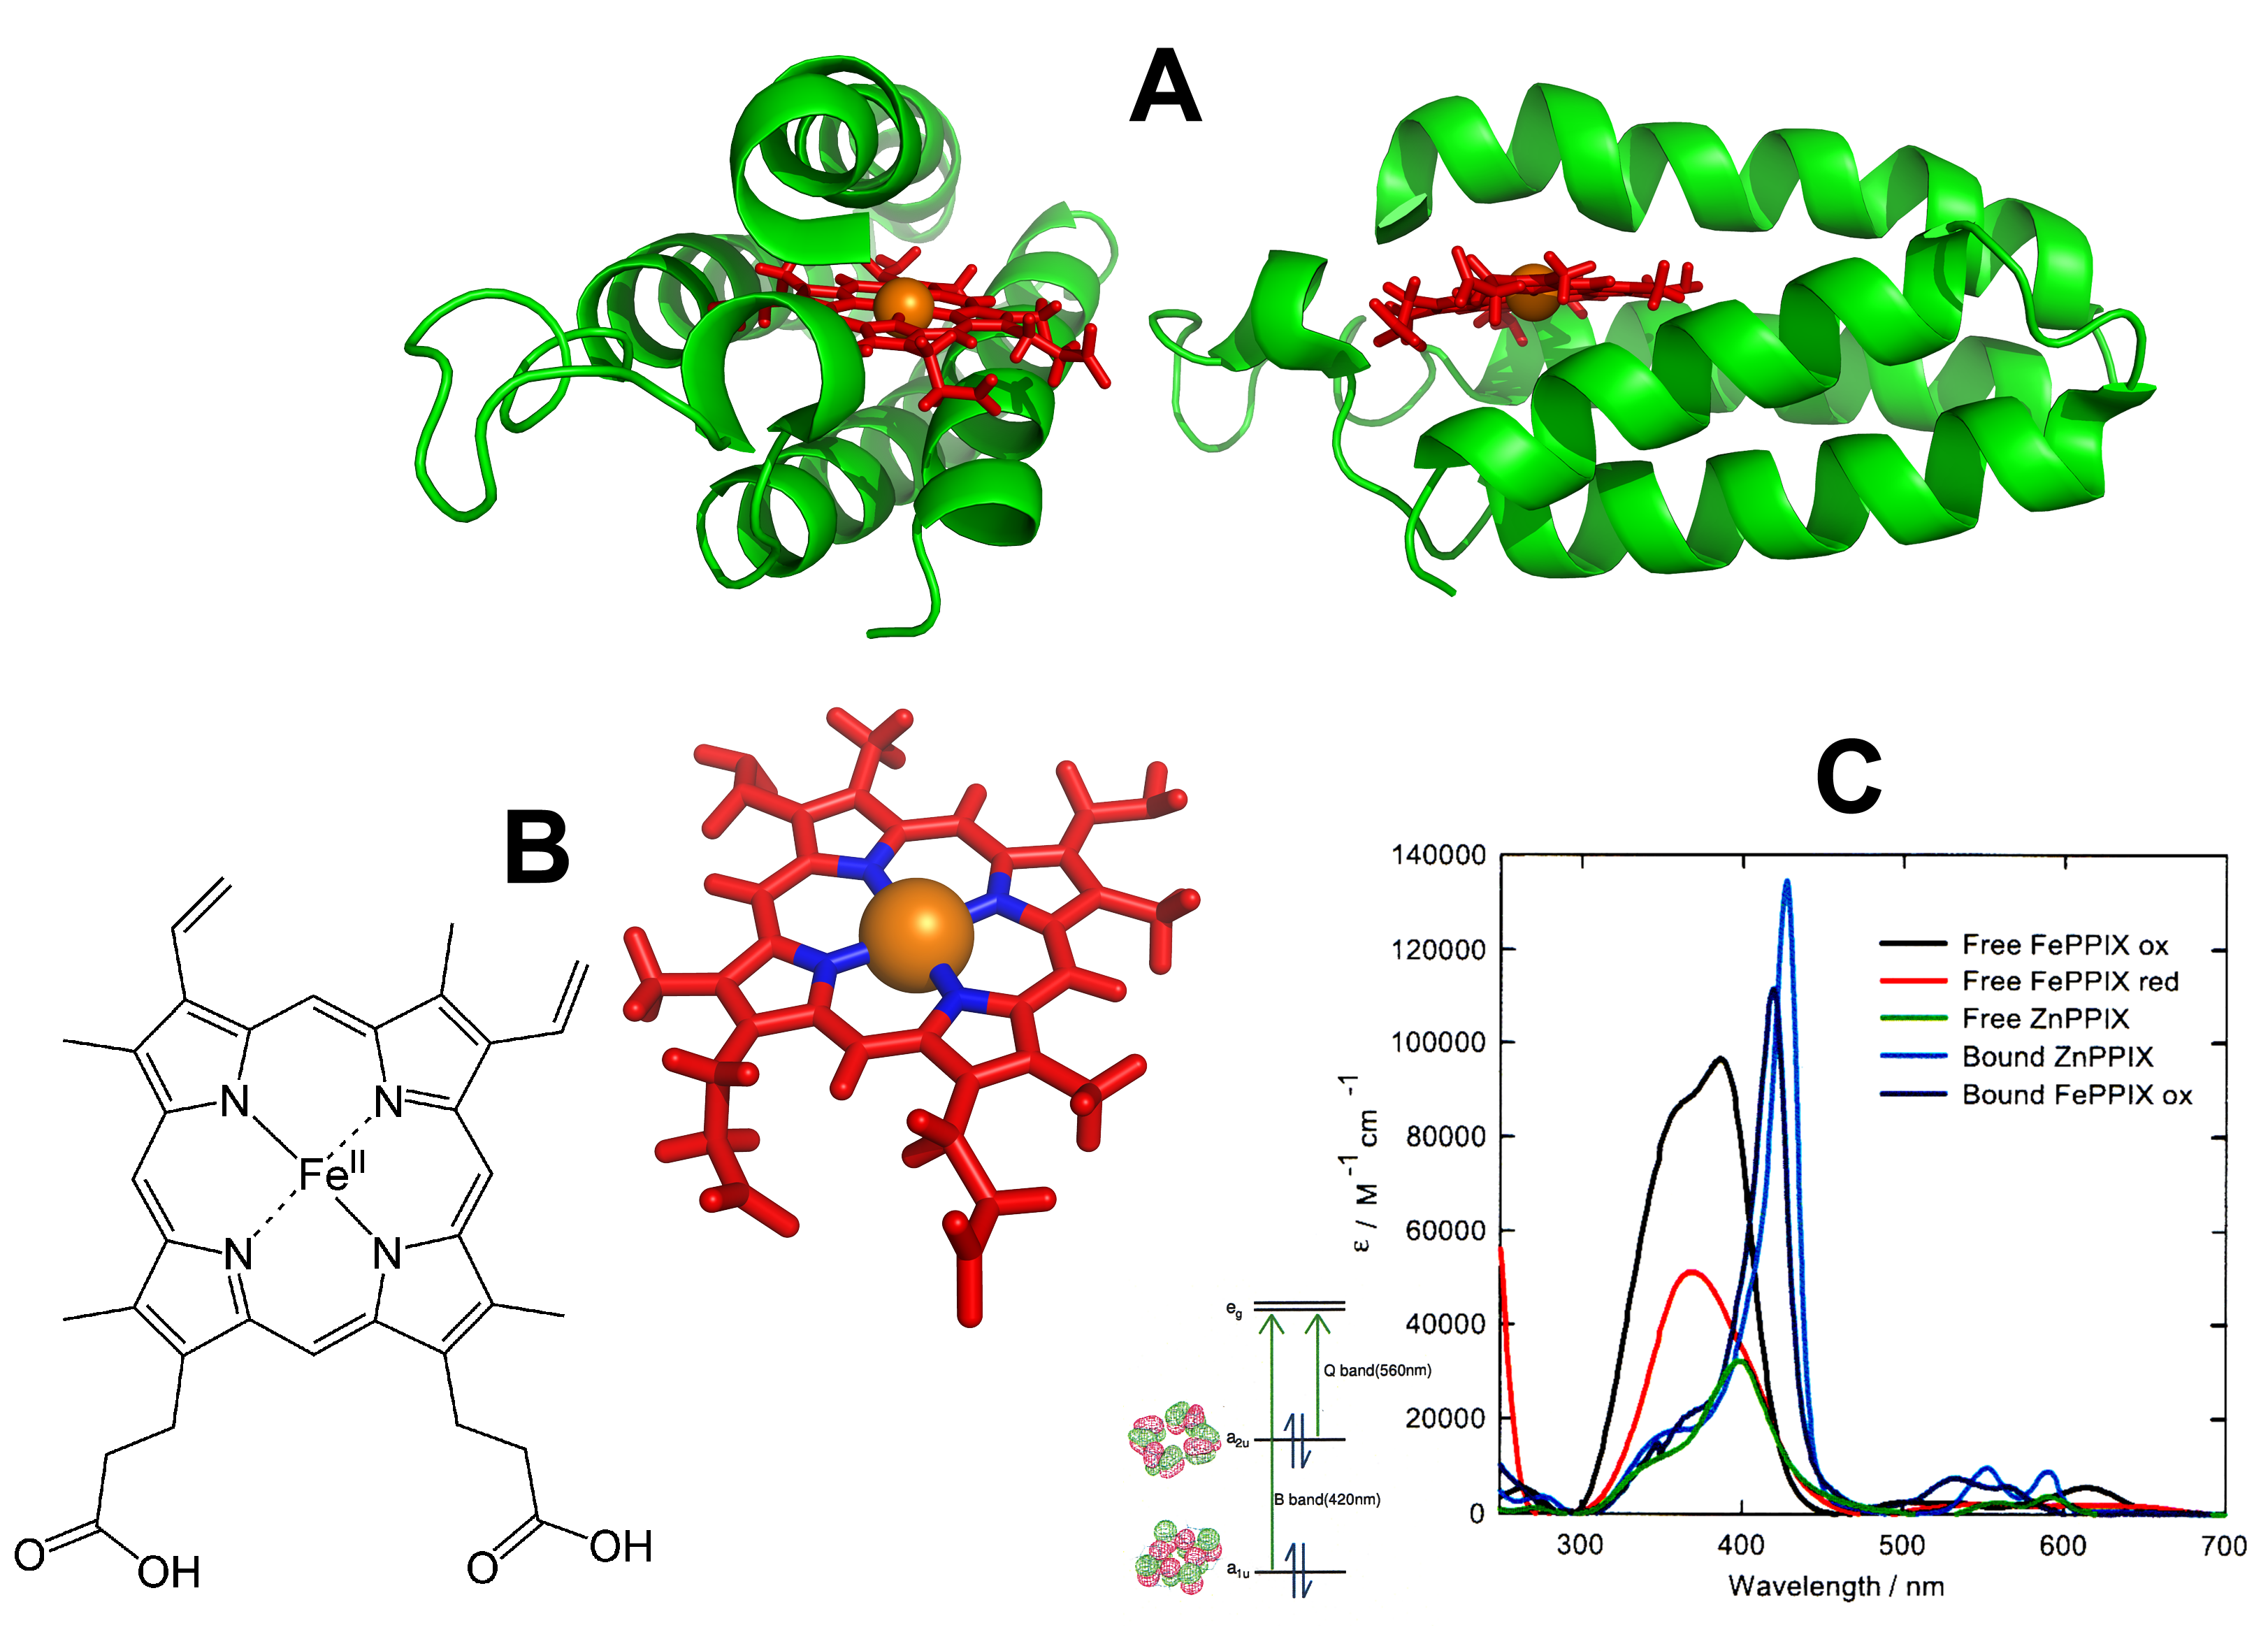
\includegraphics[width=137.4mm]{Images/haemStructure.png}
	\caption[Haem Structure]{A fancy image.}
	\label{fig:haemStructure}
\end{figure}
\end{verbatim}

\vspace{2ex}

\begin{figure}[!th]
	\centering
	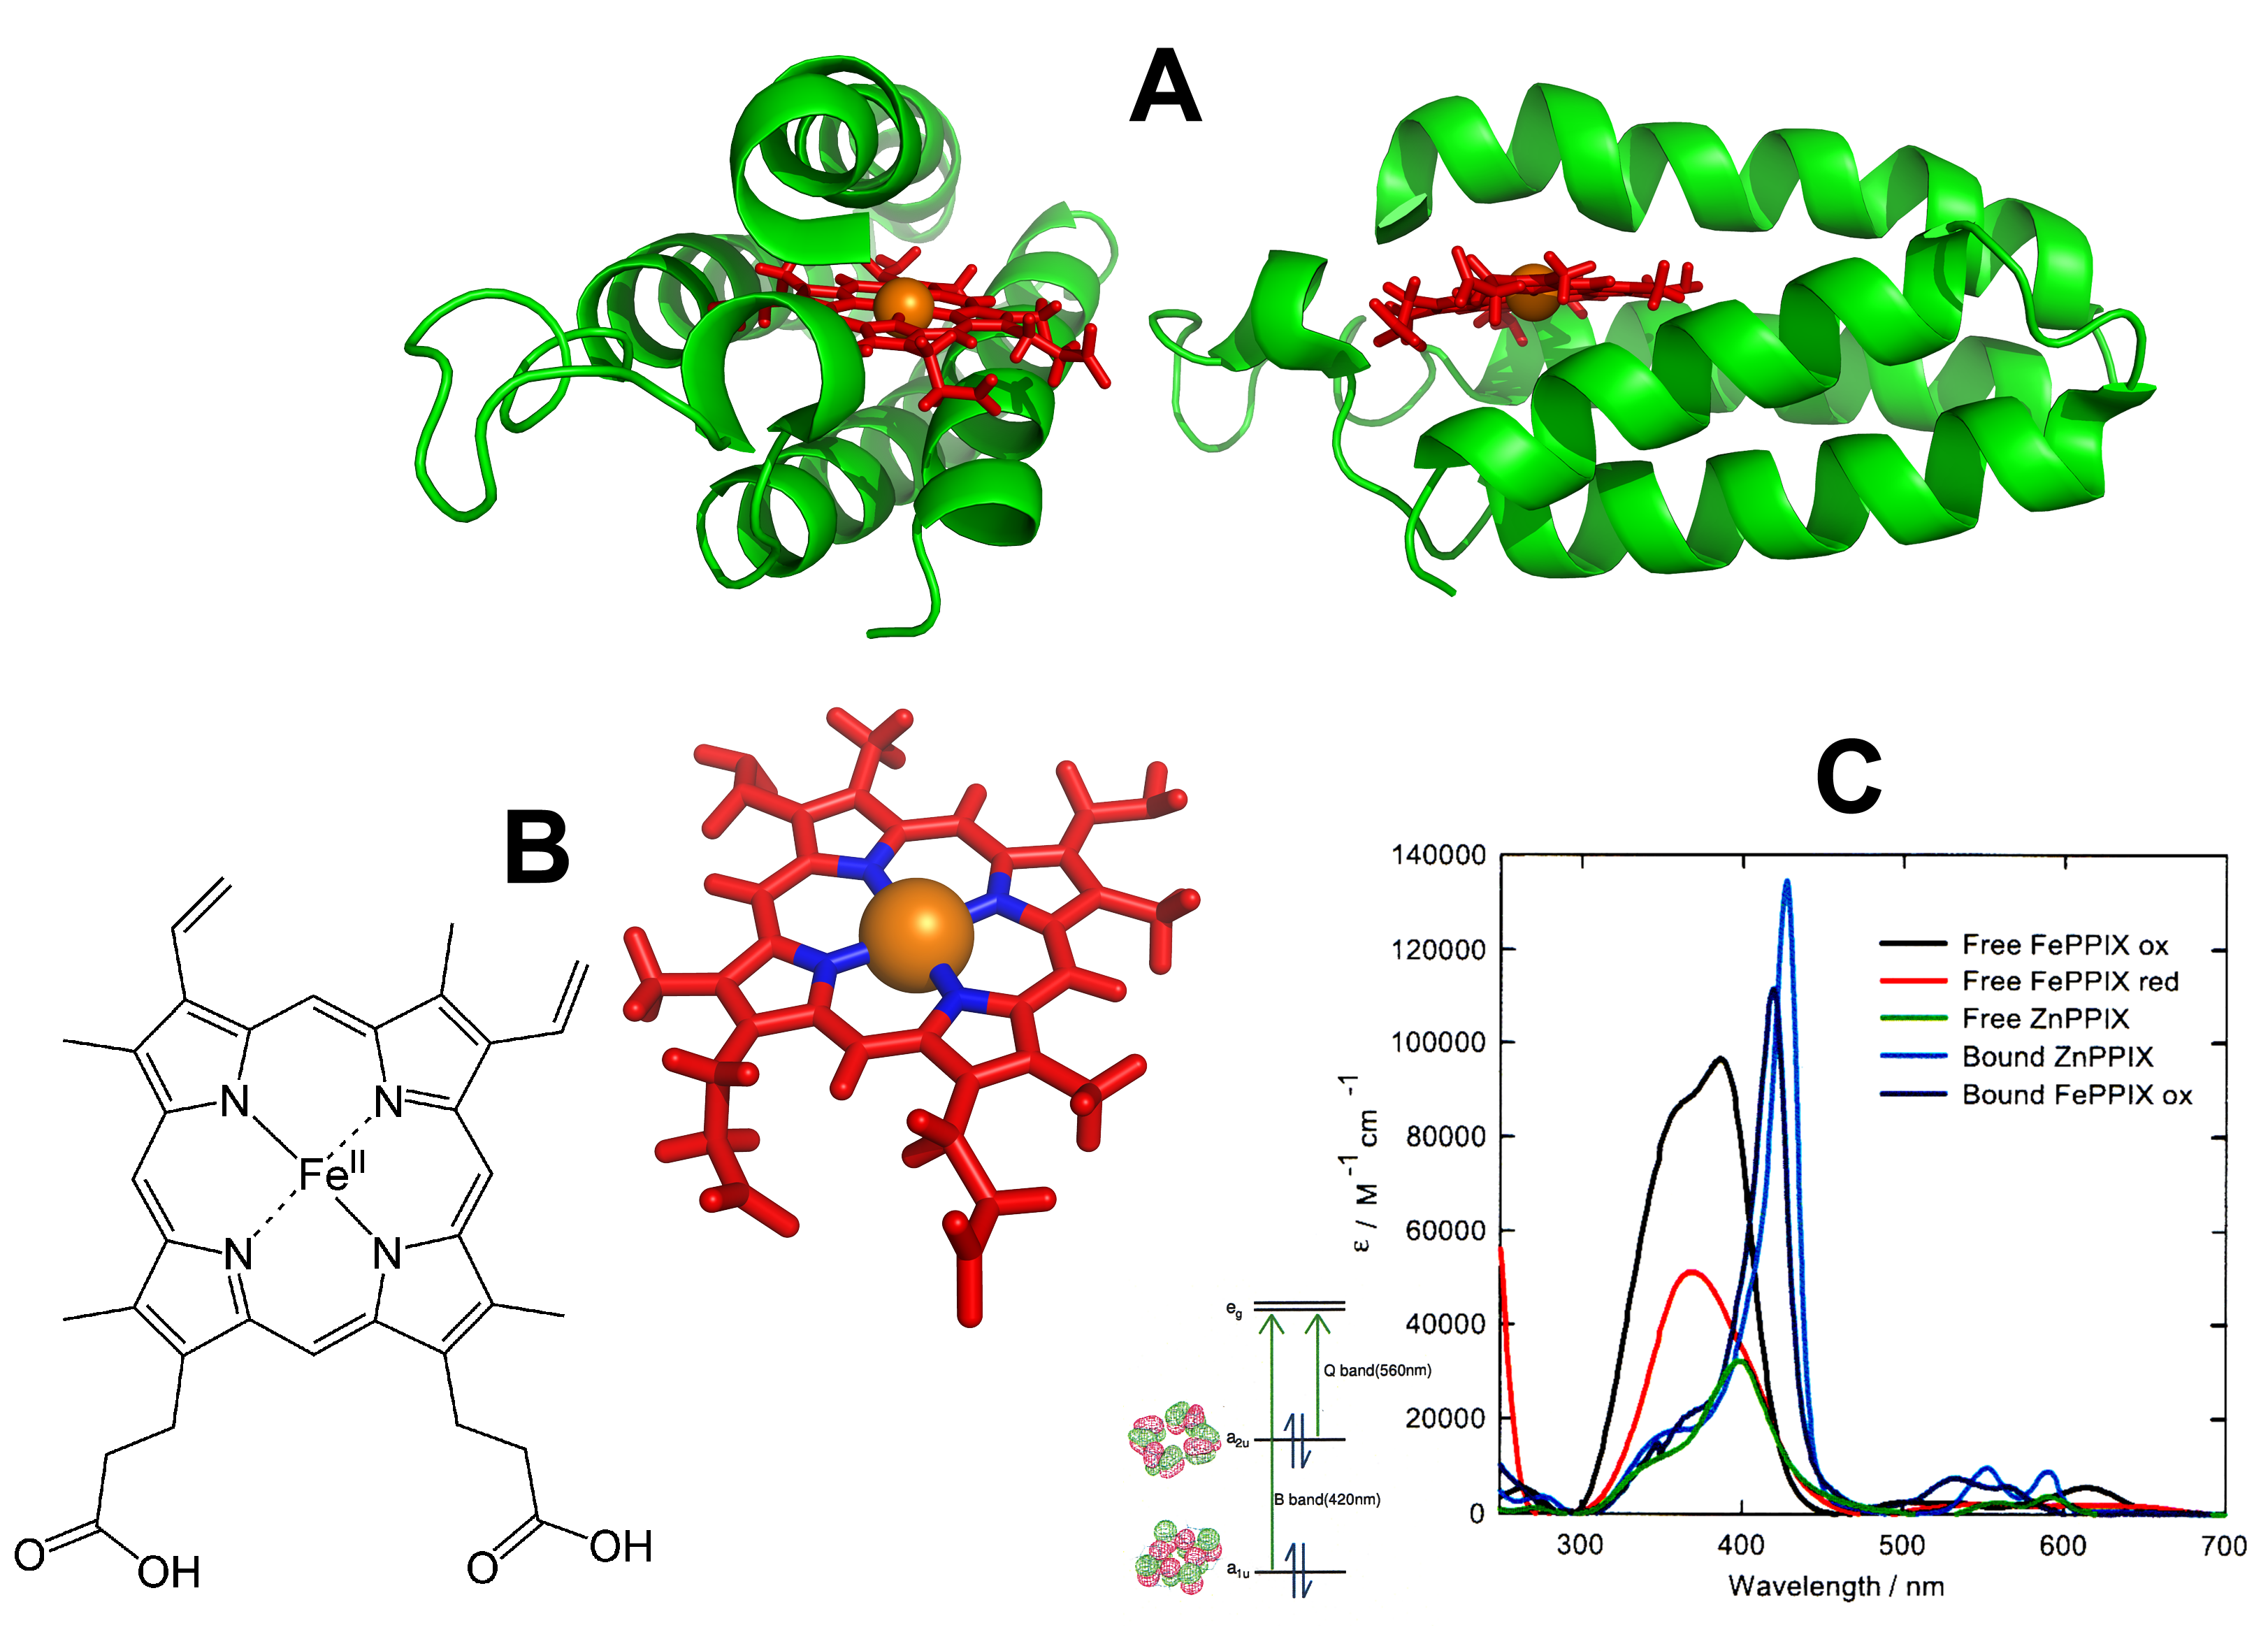
\includegraphics[width=137.4mm]{Images/haemStructure.png}
	\caption[Haem Structure]{A fancy image from Chris' Thesis.}
	\label{fig:haemStructure}
\end{figure}

In this example the command {\textbackslash}includegraphics tells LaTeX to look in the directory `Images' and incorporate the file called `haemStructure.png' into the final document while setting the width to 137.4mm.  This command can be used to resize a graphical file using the height or width parameter as shown. You must specify the units which can be pt, ex, em, mm, cm and so on. LaTeX recognises a very wide variety of standard units and graphics formats. The command is part of the graphicx package and so in the preamble you must include the command {\textbackslash}usepackage\{graphicx\}.

Many packages have been written to provide new commands. For example the `subfigure' package enables you to place separate images or files in the same figure side by side while giving them their own label. However, in this document we only concentrate on the very basics.

\section{Floating Environments}

Both tables and figures are examples of a `floating environments' which means LaTeX decides where to put them. 

The mysterious [!tbh] letters give guidance to LaTeX about roughly where the figure or table is  allowed to be, but in general they can move a long way from where you position them within your text file.  The letters in the square bracket can be t, h or b which stand for top, here or bottom.  If you don't specify any letters LaTeX defaults to [t].

LaTeX will always preserve the order in which figures appear.  If it cannot find a type setting solution, then it may move the float to it's own page, and combine it with other figures. If it still can't fit that in for some reason then it moves the float to the end of the document.  This has the effect of pushing all the remaining floating environments to the end of the document also.

The exclamation mark instructs LaTeX to ``try harder'' at putting the float where you told it to. Often you must play around to ensure the float positioning is acceptable, but usually this can be achieved by stretching or shrinking the image slightly using the size parameter, re-ordering text, judicial applications of the {\textbackslash}pagebreak command or by shouting loudly and slapping the computer monitor about. Note that it is better to resize the image using the original program that was used to create the image. Also using vector graphics can assist be useful (e.g. eps files) because they are designed to scale better.
\chapter{The Chapter on Making Chapters}
\label{sec:Chapters}

Right. LaTeX forces you to structure your document. There a series of simple commands for achieving this:

\vspace*{2ex}

{\textbackslash}chapter\{chapterName\}

{\textbackslash}section\{sectionName\}

{\textbackslash}subsection\{subsectionName\}

{\textbackslash}subsubsection\{subsubsectionName\}

\vspace*{2ex}

Easy enough. At the start of each chapter or section just issue one of these commands to name the section and LaTeX will present the chapter heading in the right style of font, which will be the same style of all the other heading names at that level of hierarchy throughout the document. In addition LaTeX assigns a number to that section. For example, this chapter was created using the command:

\vspace*{2ex}

{\textbackslash}chapter\{The Chapter on Making Chapters\} 

\vspace*{2ex}

LaTeX assigns the correct chapter number to each chapter in turn and then puts it in the table of contents, as you can see by looking at the table of contents! Easy.

\pagebreak
\section{The Section About Sections}
\label{sec:Section}
I think you're getting the hang of this. This section was created using the command {\textbackslash}section\{The Section About Sections\}. It appears in the table of contents as section \ref{sec:Section}.

\subsection{The Sub-Section About Sub-Sections}
\label{sec:SubSection}
Now you're really getting the hang of this. This subsection was created using the command {\textbackslash}subsection\{The Sub-Section About Sub-Sections\}. 

\subsubsection{The Sub-Sub-Section About Sub-Sub-Sections}
\label{sec:SubSubSection}
Now you're really getting the hang of this. but.. caught you out! This subsubsection doesn't have a number!  Ha Ha! It was created using the command {\textbackslash}subsubsection\{The Sub-Sub-Section About Sub-Sub-Sections\} in the same vein as all the other subsections/chapters etc. Here we have stopped the depth of the section numbering at the second level with the command:

\vspace*{2ex}

{\textbackslash}setcounter\{secnumdepth\}\{2\}

\vspace*{2ex}

Easy. WYSIWYM.  LaTeX does what you tell it to do. This is both a blessing and a curse.

\pagebreak
\section*{The Section About Sections That Don't Appear in the Table of Contents}
\label{sec:InvisibleSection}
Ok. Now we're throwing a spanner in the works. This section was created using the command:

\vspace*{2ex}

{\textbackslash}section*\{The Section About Sections That Don't Appear in the Table of Contents\}. 

\vspace*{2ex}

Notice how LaTeX has not assigned a number to the section and it doesn't appear in the table of contents. The effect of the * is to suppress the inclusion of a chapter, section or subsection in the automatic numbering. Easy. You can do this at any level. This is useful for things like prefaces, tables of contents or acknowledgements which you may or may not wish to have an entry in the main contents table. Up to you. It's your thesis. Don't just copy me.

\section{A Small Point About Numbering}

In this section notice how the numbering starts from where it left off before we suppressed the numbering on the previous section. Easy. WYSIWYM.
\pagebreak
\section{The Section About Internal Referencing}
\label{sec:InternalReferencing}

There are two related commands:

\vspace*{2ex}

{\textbackslash}label\{labelName\} 

{\textbackslash}ref\{labelName\}

\vspace*{2ex}


The {\textbackslash}label\{\} command allows you to create a label in a particular environment\footnote{That's right. Chapters, Sections and sub-sections etc are environments!}. The label won't appear in the final document. It's just a label which makes it easy to refer back to any particular environment elsewhere in the document. The {\textbackslash}ref\{\} command enables you to insert a reference anywhere in the document to any label in the document.  For example this is section \ref{sec:InternalReferencing}. The names you use in a label can be anything you like but musn't contain whitespace or special characters. I used the two commands:

\vspace*{2ex}

{\textbackslash}label\{sec:InternalReferencing\}

{\textbackslash}ref\{sec:InternalReferencing\}.

\vspace*{2ex}

The astute among you will realise that LaTeX has to read the document several times. Once to find the labels and then again to populate the references with the correct numbers. So you have to compile a latex document twice to get the referencing right. If there is a missing label or you refer to something that doesn't exist then latex inserts a convenient ? at that point. So hunting for queries is useful way of finding broken references. Latex issues warnings when it finds broken references.

As you create a document you will find yourself putting labels in all over the place so choose a sensible naming convention to help you remember the label names.

Each type of environment (equations, figures, tables, sections etc) has its own independent numbering system.  So when you choose your label name it's a good idea to have an identifier for that type of environment.  I have my own convention for label names which I use to help me remember references. E.g.   sec:SectionAboutCats. Eqn:EquationAboutCats,  Fig:FigureAboutCats and so on. This means you can differentiate between referring to the section or the figure more easily, even though they are about the same thing.

So Internal Referencing is a doddle. Easy!
\chapter{External Referencing}

Referencing is usually performed using a separate program called BibTex.  This program understands the file format .bib.

To create a reference within your document first you must create a .bib file by exporting your list of references from which ever referencing software you used, such as endnote, mendeley or whatever you use.

You can refer to an entry in the .bib file using the {\textbackslash}cite\{ref:Name\} command. the identifier `ref:Name' is the unique identifier which is the first line of each item included in your bibliography file.

For example, open the file LaTexCourseBib.bib in the bibliography directory. The first entry has the identifier `Horcas2007'.  This can be invoked as follows:


\begin{verbatim}
For example, this interesting fact\cite{Horcas2007}, is a cracking example.
\end{verbatim}

For example, this interesting fact\cite{Horcas2007}, is a cracking example.

During compilation latex and bibtex co-operate. During the first compilation latex generates a list of references that it needs.  During the second compilation bibtex populates the details from the .bib file into a shorter, ordered .bib file. The third compilation inserts markers at the right place in the main file and the fourth compilation generates the final list of references. Thus the compilation sequence is latex, bibtex, latex, latex.

The style of the referencing format can be changed using the command {\textbackslash}bibliographyStyle\{\}. e.g. the style used in this document is cjfthesisv1.bst which is invoked by 

\begin{verbatim}
\bibliographystyle{Bibliography/cjfthesisv1}
\end{verbatim}

The location of the list of references in the document is specified by issuing the {\textbackslash}bibliography\{\} command which also specifies the master bibliography file.

\begin{verbatim}
\bibliography{Bibliography/LaTeXCourseBib}
\end{verbatim}




\chapter{Organising Your Files}
One of the drawbacks of word is that the figures and tables are included within the document which becomes very very clunky quite quickly and once it reaches around 100Mb it becomes unwieldy and hard to export. One of that advantages of LaTeX is that the files are all text files and so are very light on resources and are easy to email around the place.

However, sometimes it can be difficult to navigate through a single text file, so if you had a huge document then it becomes difficult to find your way around.  One way of circumnavigating this problem is to break the file up into smaller files. As long as LaTeX knows where to look you can have a file for each logical sub-division of your document.

Therefore it is worth spending a bit of time at the beginning of a large project deciding how you wish to break up your LaTex Files and organise them neatly and tidily.  You can then tell LaTex where to look for the files using the following command:

\vspace*{2ex}
{\textbackslash}include\{fileName\}
\vspace*{2ex}

\pagebreak
\section{Linking a File}
We are now going to copy part of the tutorial file into a separate files and link it the main file.  Because this could go wrong it is sensible to back up tutorial.tex as something else. So save a copy called `tutorialOriginal.tex' for safe keeping. Then follow the following instructions.

\begin{enumerate}
\item Create a new file called MyFirstPage.tex
\item Select and Cut out the first chapter of Tutorial.Tex
\item Paste the first chapter into MyFirstPage.tex
\item Save both tutorial.tex and MyFirstPage.tex
\item Then add {\textbackslash}include\{MyFirstPage\} in tutorial.tex where the text used to be before you cut it out. We don't need to add the `.tex' because LaTeX can only include `.tex' files.
\item compile tutorial.tex and view the PDF
\end{enumerate}

The final PDF should look exactly the same as it was! except we now have a separate file for one of the chapters.

\pagebreak
\section{Creating A Class File}
We can also save our preamble in a separate file called a class file. This makes your main document much easier to understand.  To make it work we need to use the {\textbackslash}LoadClass\{\} command as follows: 

\begin{enumerate}
\item Create another new file and save it as TutorialStyle.cls
\item Copy the preamble of tutorial.tex into the new file. Starting with the {\textbackslash}documentclass{} command and copy right up to, but not including, the {\textbackslash}begin{document} command. Delete the preamble in the original document.
\item Save TutorialStyle.cls and tutorial.tex
\item Modify the first line of TutorialStyle.cls by replacing the word `document' with the word `Load'.
\item Add a new first line of tutorial.tex to use your new style class {\textbackslash}documentclass\{TutorialStyle\}
\item Save both files.
\end{enumerate}

\subsection{Sanity Check}

The first line of TutorialStyle.cls should now be:

\begin{verbatim}
\LoadClass[12pt, oneside, a4paper]{book}
\end{verbatim}
\vspace{2ex}

The first line of tutorial.tex should be:

\begin{verbatim}
\documentClass{TutorialStyle}
\end{verbatim}
\vspace{2ex}

We have just created what is called a style file. You can use this style file as a generic preamble for other documents as well. Compile tutorial.tex.  Nothing should have changed in the final PDF.


\pagebreak
\section{The Structure of this Document}

Lets now look at how I've organised this document. It is identical to my thesis because it started out life as my thesis. I usurped the structure and simply replaced the headings and content to make a kind of reference manual for this introductory course. This document therefore is three things:

\begin{enumerate}
\item An example thesis structure to work from.
\item The LaTeX files which were used to create it can be used as a template for a thesis.
\item It is also a convenient introductory latex manual!
\end{enumerate}

\vspace*{2ex}
Groovy huh?

\section{The Master File}

There is a master file where LaTeX begins the compilation procedure. This contains the {\textbackslash}documentclass command needed to set the ball rolling. Within the file there are a series of {\textbackslash}include\{\} commands, one for each Chapter, which tell LaTeX where to find the files containing each chapter.

The subfiles cannot be compiled on their own because they do not contain the {\textbackslash}documentclass, {\textbackslash}begin\{document\} or {\textbackslash}end\{document\} commands. Lets us look in more detail at the master file and we will learn some new LaTeX commands.

\singlespacing
\pagebreak
\begin{verbatim}
\documentclass{Style/LatexCourseStyle}

\begin{document}
\setcounter{secnumdepth}{2}
\setcounter{tocdepth}{1}

\frontmatter
\onehalfspacing
\thispagestyle{empty}

\begin{center}
\vspace*{\stretch{1}}

\hrule height 2pt
\vspace*{2ex}
{\Huge\textbf{Towards the Ability to Make Super Duper LaTeX Documents}\par}
\vspace*{2ex}
\hrule height 2pt
\vspace*{10ex}
{
\includegraphics[height=40mm]{Images/UnivShield}\par}
\vspace*{10ex}
{\large\textbf{Christopher~James~Forman}\par}
\vspace*{2ex}
{\large{Department Of Chemistry}\par}
\vspace*{2ex}
{\large{University of Cambridge}\par}
\vspace*{5ex}
{\large{This dissertation is submitted for the degree of \textit{Doctor of Philosophy}}\par}
\vspace*{5ex}
{\large{\today}\par}

\vspace*{\stretch{2}}
\end{center}
\chapter*{Declaration}

\vfill

This dissertation is the result of my own work and includes nothing which is the outcome of work done in collaboration except where specifically indicated in the text. It is not substantially the same as any that I have submitted for a degree or diploma or other qualification at any other University and no part has already been, or is concurrently being, submitted for any degree, diploma, or other qualification. It does not exceed 60,000 words, including tables, footnotes, bibliography and appendices.\par

\vspace{10ex}

\begin{flushright}
Signature: \rule[0pt]{60mm}{0.5pt}

\vspace{5ex}

Date: \rule[0pt]{60mm}{0.5pt}
\end{flushright}

\vfill
\chapter*{Acknowledgments}
\subsection*{Family}
Mum. Dad. Pet Dog.

\subsection*{Scientific Collaborations}
Dr A.N.Other at uni of blah for samples and instrument time etc. My Amazing Lab Chums.

\subsection*{Scientific Support}
My amazing lab chums.

\subsection*{General Assistance}
Cleaner, My amazing lab chums.

\subsection*{Financial Support}
Bank, Tax payer. My amazing lab chums.

\subsection*{Moral Support}
My Amazing Lab chums.

\subsection*{Academic Inspiration}
Netwon, My super. My Amazing Lab Chums.

\subsection*{Everyone else}
My Amazing Lab Chums.

\chapter*{Summary}
This document is a handbook for introducing you to LaTeX. It contains a bit of background about the history and philosophy of LaTeX.  However, it concentrates on providing a guided practical introduction to the basic techniques such as 
\begin{itemize}
\item Lists
\item Mathematical and chemical equations
\item Tables
\item Figures
\item Chapters and Sections
\item Linking to other files in large documents
\item Referencing
\end{itemize}

The handbook is also presented in the style of a thesis. This means that source files provided on the introductory course and available from the department web page are a convenient template for a thesis.

More details on specific aspects of LaTeX can be found at the departmental LaTeX page which can be found here:

 http://www-ch-int.ch.private.cam.ac.uk/latex/about

\chapter*{Abbreviations}

\begin{longtable}{r >{\rule{0pt}{3ex}}l<{\rule[-1.5ex]{0pt}{0pt}}}
ADP & Adenosine Diphosphate\\
(nc/c)AFM & (non-contact/conducting) Atomic Force Microscopy\\
ATP & Adenosine Triphosphate \\
\end{longtable}
\tableofcontents
\listoftables
\listoffigures

\mainmatter
\renewcommand{\sectionmark}[1]{\markright{\thesection \ #1}{}}
\chapter{Overview}
\label{chap:overview}
\section{LaTeX: The answer to everything.}
LaTeX is typsetting program that takes an input file of marked up text and then, with a user defined set of rules, typesets a beautifully crafted output file that can be easily printed (e.g. a pdf). 

\subsection{Advantages}

The advantages of this method are manifold:

\begin{itemize}

\item Use any text editor to view the source document.
\item More time can be spent working on the content and not worrying about how text or figures interact in the layout until later on.
\item LaTeX uses consistent rules throughout a document
\item LaTeX sorts out basic typesetting automatically
\item Changes can be introduced globally with very little effort
\item Document structure is explicit
\item Documents can be professionally typeset and look great
\item You are forced to structure your documents correctly.
\item Mathematical equations, like $E=mc^2$ or $\imath\hbar\frac{\partial}{\partial t}\Phi (x, t) = \hat{H}\Phi (x, t)$ can be produced almost as fast as typing (if you know the commands!).
\end{itemize}

\subsection{Disadvantages}
The disadvanatges of this method are also manifold:
\begin{itemize}
\item You don't see the output as you go.
\item Steep learning curve.
\item Documents are harder to edit by a second author (unless they are adept at LaTeX too). This can be mitigated using version control, which makes group authoring processes superior to word.
\item The program never works quite the way you want it to and learning how to influence it can be problematic and subtle.
\item Although intended to save work the principle of 'conservation of work' means that you simply transform problems associated with WYSISYG approaches to problems associated with WYSIWYM approaches!
\item You can go blind trying to determine the difference between wiggly and smooth brackets if your editors font isn't large enough.
\end{itemize}

\subsection{On balance?}
If it's so rubbish, why use LaTeX?

\begin{itemize}
\item Large documents are much more easily handled. 
\item In general it is quicker to debug a LaTeX document than typeset an entire thesis manually. 
\item Technical information such as tables, equations and figures are integrated much more smoothly than with word.
\end{itemize}

\section{How does it work?}

The raw text is interspersed with commands, preceded by a \textbackslash, which tell LaTeX what to do with the text. For example you can \textbf{make it bold}, \emph{italic}, or \underline{underlined} with the commands {\textbackslash}textbf\{\}, {\textbackslash}emph\{\} or {\textbackslash}underlined\{\}. More on commands in a moment...



\chapter{My First Page}

\section{The Very Beginning}
The very simplest LaTeX document might look like this:

\begin{verbatim}
\documentclass[a4paper,12pt]{article}
\begin{document}
Hello World.
\end{document}
\end{verbatim}

\pagebreak
\thispagestyle{empty}
Hello World.
\pagebreak
\subsection{Break Down}
What's all the gobbledegook around my simple message???

In LaTeX we intersperse text and commands.  Commands are preceded by a \textbackslash. For example the first line in a LaTeX document \underline{\textbf{\emph{must}}} be:

\begin{verbatim}
\documentclass[options]{class}
\end{verbatim}

Where the word ''class'' may be substituted for one of many things such as: article, proc, minimal, report, book, letter, memoir, slides, beamer.

Similarly, and completely generally in LaTeX speak, the square brackets denote the existence of optional parameters. Each individual command can take its own parameters and for the ''{\textbackslash}documentclass'' command there are options for controlling font size, font family, landscape, oneside, twosided, page size and so on. These options will persist throughout the entire document. For example the document class command for this document, (which is likely to be like the one you would use for a thesis), would be:

\begin{verbatim}
\documentclass[12pt, oneside, a4paper]{book}
\end{verbatim}

Other options include:

\begin{itemize}
\item {10pt, 11pt, 12pt (default is 10pt).}
\item {letterpaper, legalpaper, a4paper, executivepaper, a5paper, b5paper}
\end{itemize}
and so on.

\pagebreak
\section{Can I start typing please?}

After we have set up the document we can start actual work on our document. So we must tell LaTeX that what follows is to be interpreted as a document.  The command {\textbackslash}begin can take many different parameters and is a command to enter what is known, in LaTeX speak, as 'an environment'. Thus the commands:
\begin{verbatim}
\begin{document}

\end{document}
\end{verbatim}

tells LaTeX to enter and leave the document environment, and thus constitute the outer limits of our document file. Other environments include the equation environment, the itemize environment, the figure environment and so on. These will be encountered in due course.

Every part of the LaTeX file is therefore within an environment of specific type and the content within each environment consists of commands or text.

That's basically it.

So let's get on with it shall we...

\pagebreak
\section{The ground rules}
\begin{quote}
Hold on, hold on, hold on my son.

First the lessons.

Then the fun!
\end{quote}
Dr Seuss.

\subsection{Spaces}
Whitespace characters, such as blank or tab, are treated uniformly as space by LaTeX. Several consecutive whitespace characters are treated as one single space. Whitespace at the start of a line is generally ignored, and a single line break is treated as whitespace. An empty line between two lines of text defines the end of a paragraph. Several empty lines are treated the same as one empty line. The text below is an example.

\begin{verbatim}
It does not matter whether you
enter one or several             spaces
after a word. The final result will be typeset beautifully
according    to     precise rules.




An empty line starts a new
paragraph. Note the indentation on the first line of the paragraph, 
except at the beginning of the section. 
\end{verbatim}

\vspace*{2ex}
\vspace*{2ex}

It does not matter whether you
enter one or several             spaces
after a word. The final result will be typeset beautifully
according    to     specific rules.




An empty line starts a new
paragraph. Note the indentation on the first line of the paragraph, except at the beginning of the section. 

\pagebreak
\subsection{Special Characters}
The symbols 

\# \$ \% \textasciicircum{} \& \_ \{ \} \~{} \textbackslash

are reserved characters that either have a special meaning under LaTeX or are unavailable in all the fonts. If you enter them directly in your text, they will normally not print, but rather make LaTeX do strange things.

To overide the special meanings of these symbols and allow them to produced within your text you may use the following sequences:
\begin{verbatim}
\# \$ \% \textasciicircum{} \& \_ \{ \} \~{} \textbackslash
\end{verbatim}

Other symbols and many more can be printed with special commands in mathematical formulae or as accents.

The backslash character '\textbackslash' cannot be entered by adding another backslash in front of it ( \textbackslash\textbackslash); because this sequence means ''linebreak''.

The command \textbackslash\~{}\{\} produces a tilde which is placed over the next letter. For example \textbackslash\~{}\{n\} gives \~{n}. To produce just the character \~{}, use \textbackslash\~{}\{\} which places a \~{} over an empty box.

Similarly, the command \textbackslash\textasciicircum{} produces a hat over the next character, for example \textbackslash\textasciicircum\{o\} produces \^{o}.

\pagebreak
\section{Preamble}
After the {\textbackslash}documentclass command we add ''preamble''. Here we load special features that we will use throughout our document to expand on the basic capabilities of LaTex. These are contained in units called ''packages'' which we can tell our LaTeX compiler to download by using the command ''{\textbackslash}include\{packageName\}''. 

There are many repositories of such packages on the web. Your compiler generally knows where to look and most standard packages are included with any install. For example, to include a special set of typesetting instructions to handle chemical equations we can grow our simple document with a single command like this:

\begin{verbatim}
\documentclass[a4paper,12pt]{article}
\usepackage[version=3]{mhchem}
\begin{document}
Hello World!

We all need \ce{H2O}.

I'm less fussed about \ce{^{235}_{92}U+}.

\end{document}
\end{verbatim}

\vspace{2ex}

\pagebreak
\thispagestyle{empty}
Hello World!

We all need \ce{H2O}.

I'm less fussed about \ce{^{235}_{92}U+}.
\pagebreak

Here we have loaded a package called: "`mhchem"' which took the option ''[version=3]''. This is a package for drawing chemical equations easily and it has it's own instruction manual which you can follow easily. It is included in the bundle of files for this course.

Other things we can do in the premable within LaTeX are to redefine existing commands or create our own personal commands. These can be stored in a file called the 'style file' which we can load at the beginning of our document, in place of our documentclass. More about this later on...


\subsection{Comments}
It is often useful to comment your LaTeX documents. You can leave yourself amusing, sarcastic messages that won't get printed out in the final document. Use this to make your own notes as the course progresses.

To get a comment use the \% command, which tells LaTeX to ignore the rest of the line, the line break and all the white space at the beginning of the next line, for example, we may add to our continually evolving document...

\begin{verbatim}
\documentclass[a4paper,12pt]{article}
\usepackage[version=3]{mhchem}
\begin{document}
Hello World!

%All humans need water and I would like 
%to include this concept in my arguments.
We all need \ce{H2O}.

%Uranium 235 is toxic, which is why I don't want to consume it... 
I'm less fussed about \ce{^{235}_{92}U+}.

\end{document}
\end{verbatim}

\vspace{4ex}
Hello World!

%All humans need water and I would like to include this concept in my arguments.
We all need \ce{H2O}.

%Uranium 235 is toxic, which is why I don't want to consume it... 
I'm less fussed about \ce{^{235}_{92}U+}.

\pagebreak
\section{Compiling}
Once the document is finished you can compile it. Your compiler will depend on the platform that you use. In the PWF we are using winEDT to edit the documents (a LaTeX front end) and texlive2008 which is the compiler itself. I use MiKTex and the front end texCenter.  There is no need to use a front end. If you prefer you can use a simple text editor and a command line.

the recommended distributions are:
\begin{itemize}
\item MiKTeX or TeX Live for Windows
\item TeX Live for Unix/Linux
\item MacTeX or TeX Live for Mac OS.
\end{itemize}

Once you have installed your software and got it working, written your source code and tried to compile it, there will nearly always be something wrong with your file. 

Any errors will be highlighted in the console window or error output box of your front end.  Some front ends dump the running commentary which LaTeX produces into a text file for easy reading afterwards.

In a compile attempt (successful or otherwise) LaTeX may produce the following files:

projectname.aux

projectname.bbl

projectname.lof

projectname.lot

projectname.txt

projectname.toc

projectname.dvi

These are interim files (toc= table of contents, bbl = bibliography etc). To be honest I have no idea what half of these things contain.  You only need the .tex file and a compiler with the right packages installed to produce them again.

Some versions of LaTeX only produce DVI files and you then need to convert the dvi file to a PDF or download a dvi viewer. You can also convert DVI files to PS files and then view them.  The good thing about front ends is that you can set them up to produce PDFs directly.

OK. So we have now produced a silly document but we understand it.  Now lets get on with learning how to make our own documents.



\chapter{Lists}
Lists are great.  The command {\textbackslash}begin\{\} can be used to enter a list environment.  For example:

\begin{verbatim}
\begin{itemize}
\item cat
\item dog
\item horse
\end{itemize}
\end{verbatim}

Produces:

\begin{itemize}
\item cat
\item dog
\item horse
\end{itemize}

\pagebreak
We can also replace the bullet points with numbers using the enumerate keyword.

\begin{verbatim}
\begin{enumerate}
\item cat
\item dog
\item horse
\end{enumerate}
\end{verbatim}

\begin{enumerate}
\item cat
\item dog
\item horse
\end{enumerate}

\pagebreak
and we can use the description keyword which does this:
\begin{verbatim}
\begin{description}
\item[Cat] a lovely furry creature with a cute nose and whiskers.
\item[Dog] Another furry creature that smells rather well; 
           its olfactory power stems from its nasal dampness.
\item [Horse] A large stinky creature with sideways facing eyes.
\end{description}
\end{verbatim}

\begin{description}
\item[Cat] a lovely furry creature with a cute nose and whiskers.
\item[Dog] Another furry creature that smells rather well; its olfactory power stems from its nasal dampness.
\item [Horse] A large stinky creature with sideways facing eyes.
\end{description}
\chapter{Maths Equations}

\section{Producing Beautiful Looking Mathematics}

One of the best features about LaTeX is `maths mode'.  For example the schrodinger equation can be produced as follows:

\vspace*{2ex}

\begin{center}
\begin{math}
\imath\hbar\frac{\partial}{\partial t}\Phi (x, t) = \hat{H}\Phi (x, t)
\end{math}
\end{center}

\vspace*{2ex}

\begin{verbatim}
\begin{math}
\imath\hbar\frac{\partial}{\partial t}\Phi(x,t)=\hat{H}\Phi(x,t)
\end{math}
\end{verbatim}

There are a number of ways to switch on maths mode.  The first, as above, is with the {\textbackslash}begin\{math\} environment. You can also enter mathmode inline using the \$ symbol. For example typing in \$y=ax\textasciicircum{}2+bx+c\$ yields $y=ax^2+bx+c$.  Another way is to enter the equation environment which enables you to number equations so you can then refer to them later in the text.

\begin{equation}
y(t)= \sin \left(\frac{{\alpha}t}{2\pi} + \phi_0\right)
\label{eqn:MadeUpNonsense}
\end{equation}

\vspace*{2ex}
\begin{verbatim}
\begin{equation}
y(t)= \sin \left(\frac{{\alpha}t}{2\pi} + \phi_0\right)
\end{equation}
\end{verbatim}.

\section{Basic Maths Mode}
Once in maths mode there is a kind of text based code for writing down your equations.  Here are the most basic symbols to get you going.
\begin{center}
\begin{tabular}{cc}
\toprule
Final Result & LaTeX Code \\
\cmidrule(){1-2}
$a+b$ & a+b \\
$a-b$ & a-b \\
$ab$ & ab \\
$a*b$ & a*b \\
$a \times b$ & a {\textbackslash}times b \\
$a \cdot b$ & a {\textbackslash}cdot b \\
$\frac{a}{b}$ & {\textbackslash}frac\{a\}\{b\} \\ 
$a^b$ & a\textasciicircum{}b \\
$a_b$ & a\_b \\
$\sin a$ & {\textbackslash}sin a  (same for cos, tan)\\
$ sin a$ & sin a \\
$\sqrt{a}$ & {\textbackslash}sqrt\{a\} \\
$\left( a \right) $ & {\textbackslash}left( a {\textbackslash}right)\\ 
$\left[ a \right]$ & {\textbackslash}left[ a {\textbackslash}right]\\ 
$\alpha$ & {\textbackslash}alpha \\
$\pi$ & {\textbackslash}pi \\
\bottomrule
\end{tabular}
\end{center}

A full treatise on maths mode is not practical here. There are lots of online tutorials and summaries of symbols. It just takes a bit of practice and you can build up equations really easily. It's straight forward to learn new stuff once you've done it a few times.

\pagebreak
\section{Equation Arrays}
Sometimes you need to arrange several equations vertically, referencing individual lines separately and aligning the equations on the $=$ sign. This can be achieved with equation arrays as follows:

\begin{eqnarray}
A\left( x\right) & = & \frac{x^2+2x+1}{x+1} \\
& = & \frac{\left(x+1\right)\left(x+1\right)}{x+1} \nonumber\\
& = & x+1 \nonumber\\
B(x,t) & = & \frac{e^{\left(\imath\omega_0 t + kx\right)}}{4\pi\epsilon_0}
\end{eqnarray}

\begin{verbatim}
\begin{eqnarray}
A\left( x\right) & = & \frac{x^2+2x+1}{1+x} \\
& = & \frac{\left(x+1\right)\left(x+1\right)}{1+x} \nonumber\\
& = & x+1 \nonumber\\
B(x,t) & = & \frac{e^{\left(\imath\omega_0 t + kx\right)}}{4\pi\epsilon_0}
\end{eqnarray}
\end{verbatim}

\begin{itemize}
\item Note the \& symbols. This tells LaTeX where to align the equations. There must be the same number of \& symbols in each line.
\item Note the \textbackslash\textbackslash ~at the end of each line except the last one. This symbol tells LaTeX to add another row in the array.  If you put it on the last line you get an empty row at the bottom of the array.
\item Note the {\textbackslash}nonumber command which suppresses line numbering for that line.
\item Note that equation number carries on from equation \ref{eqn:MadeUpNonsense} in the previous section.
\end{itemize}

\section{Maths Packages}

Maths mode comes as standard in LaTeX, however you can download packages that buff up your maths symbol set. For example neat vector notation comes in the package `vector'. e.g. {\textbackslash}uuvec\{T\} yields $\uuvec{T}$.

\begin{verbatim}
\usepackage{amssymb}
\usepackage{amsmath}
\usepackage{vector}
\end{verbatim}


\chapter{Chemical Equations}
The mhchem package means you can do basic stuff very easily using {\textbackslash}ce\{\}. For example:

\vspace{2ex}
\begin{verbatim}
\ce{CO2 + C -> 2CO}
\ce{CO2 + C <- 2CO}
\ce{CO2 + C <=> 2CO}
\ce{A-B=C#D\sbond E\dbond F\tbond G}
\end{verbatim}
\vspace{2ex}
\begin{center}
\ce{CO2 + C -> 2CO}

\ce{CO2 + C <- 2CO}

\ce{CO2 + C <=> 2CO}

\ce{A-B=C#D\sbond E\dbond F\tbond G}
\end{center}

\vspace{2ex}
You can also use math mode within chemical equations.
\vspace{2ex}

\begin{center}
\ce{$x\,$ Na(NH4)HPO4 ->[\Delta] (NaPO3)_{$x$} + $x\,$ NH3 ^ + $x\,$ H2O}
\end{center}

\begin{verbatim}
\ce{$x\,$ Na(NH4)HPO4 ->[\Delta](NaPO3)_{$x$} + $x\,$ NH3 ^ + $x\,$ H2O}
\end{verbatim}

And you can number chemical reactions as well by using the math mode equation environment.

\begin{equation}
\ce{CO2 + C <=> 2CO}
\end{equation}

\begin{verbatim}
\begin{equation}
\ce{CO2 + C <=> 2CO}
\end{equation}
\end{verbatim}

However, this will number mathematical and chemical equations using the same number system. There is a discussion in the mhchem pdf which shows you how to number chemical and mathematical equations independently. It's a bit complex and involves you creating your own type of environment... bit beyond the intro level of this course...
\chapter{Tables}
Tables are big business in Latex.  I use these packages to help me.

\begin{verbatim}
\usepackage{multirow}
\usepackage{booktabs}
\usepackage{dcolumn}
\end{verbatim}

Here's an example table

\begin{table}[!hb]
 \centering
	\begin{tabular}{@{}rccc@{~}r@{.}l*3{r@{.}l@{~}r@{.}l}D{.}{\cdot}{2,1}}
	\toprule
	\multicolumn{1}{c}{Fibre Type}
	& N 
	& M 
	&\multicolumn{3}{c}{$L_t$ (nm)}
	&\multicolumn{4}{c}{$R_t$ (nm)}
	&\multicolumn{4}{c}{$d_t$ (nm)}
	&\multicolumn{4}{c}{${\Delta}Z_t$ (nm)}
	&\multicolumn{1}{c}{~}\\
\cmidrule(lr){1-1}
\cmidrule(lr){2-2}
\cmidrule(lr){3-3}
\cmidrule(lr){4-6}
\cmidrule(lr){7-10}
\cmidrule(lr){11-14}
\cmidrule(lr){15-18}
  SS Twisted & 5 & 4 & 313 &\multicolumn{2}{c}{(122)} & 5&7 &(1&6)  & 5&4 &(1&0)  &  150&5 &(63&1) &\multicolumn{1}{c}{~} \\
  \multicolumn{19}{c}{~}\\
  %\cmidrule(lr){3-18}
  &
  &
 	&\multicolumn{3}{c}{$L_s$ (nm)} 
 	&\multicolumn{4}{c}{$R_s$ (nm)}
 	&\multicolumn{4}{c}{$W_s$ (nm)}
 	&\multicolumn{4}{c}{${\Delta}Z_s$ (nm)}
 	&\multicolumn{1}{c}{${\Delta}Z_{e}$ (nm)}\\
\cmidrule(lr){4-6}
\cmidrule(lr){7-10}
\cmidrule(lr){11-14}
\cmidrule(lr){15-18}
\cmidrule(lr){19-19}
  SS Spiral& 32 & 7 &123&(31&6)&11&4&(3&3)&11&1&(2&6)&32&9&(22&2)&26.9\\
  SSB Spiral& 64&18 &106&(22&9)&10&8&(2&7)&9&8&(1&8)&28&2&(8&1)&22.7\\
	%\midrule
  BSS Spiral&37 &19 &110&(44&9)&13&4&(3&0)&12&9&(1&8)&27&1&(9&1)&21.5\\
	%\midrule
  SSSB Spiral&26& 6 &104&(23&9)&13&3&(2&6)&16&4&(3&4)&29&9&(11&1)&22.5\\
	\bottomrule
	\end{tabular}	
	\caption[Basic Fibre Dimensions by TEM]{A funky table from my thesis.}
	\label{tab:BasicXSBFibreDimensionsTEM}
\end{table}

\pagebreak
Here's what the code looks like:
\begin{verbatim}
\begin{table}[!hb]
 \centering
	\begin{tabular}{@{}rccc@{~}r@{.}l*3{r@{.}l@{~}r@{.}l}D{.}{\cdot}{2,1}}
	\toprule
	\multicolumn{1}{c}{Fibre Type}
	& N 
	& M 
	&\multicolumn{3}{c}{$L_t$ (nm)}
	&\multicolumn{4}{c}{$R_t$ (nm)}
	&\multicolumn{4}{c}{$d_t$ (nm)}
	&\multicolumn{4}{c}{${\Delta}Z_t$ (nm)}
	&\multicolumn{1}{c}{~}\\
\cmidrule(lr){1-1}
\cmidrule(lr){2-2}
\cmidrule(lr){3-3}
\cmidrule(lr){4-6}
\cmidrule(lr){7-10}
\cmidrule(lr){11-14}
\cmidrule(lr){15-18}
  SS Twisted & 5 & 4 & 313 &\multicolumn{2}{c}{(122)} & 5&7 &(1&6)  & 5&4 &(1&0)  &  150&5 &(63&1) &\multicolumn{1}{c}{~} \\
  \multicolumn{19}{c}{~}\\
  %\cmidrule(lr){3-18}
  &
  &
 	&\multicolumn{3}{c}{$L_s$ (nm)} 
 	&\multicolumn{4}{c}{$R_s$ (nm)}
 	&\multicolumn{4}{c}{$W_s$ (nm)}
 	&\multicolumn{4}{c}{${\Delta}Z_s$ (nm)}
 	&\multicolumn{1}{c}{${\Delta}Z_{e}$ (nm)}\\
\cmidrule(lr){4-6}
\cmidrule(lr){7-10}
\cmidrule(lr){11-14}
\cmidrule(lr){15-18}
\cmidrule(lr){19-19}
  SS Spiral& 32 & 7 &123&(31&6)&11&4&(3&3)&11&1&(2&6)&32&9&(22&2)&26.9\\
  SSB Spiral& 64&18 &106&(22&9)&10&8&(2&7)&9&8&(1&8)&28&2&(8&1)&22.7\\
	%\midrule
  BSS Spiral&37 &19 &110&(44&9)&13&4&(3&0)&12&9&(1&8)&27&1&(9&1)&21.5\\
	%\midrule
  SSSB Spiral&26& 6 &104&(23&9)&13&3&(2&6)&16&4&(3&4)&29&9&(11&1)&22.5\\
	\bottomrule
	\end{tabular}	
	\caption[Basic Fibre Dimensions by TEM]{A funky table from my thesis.}
	\label{tab:BasicXSBFibreDimensionsTEM}
\end{table}
\end{verbatim}

\pagebreak

\section{Tables Made Easy}
Here is a simple table followed by the code that produced it.

\begin{center}
\begin{tabular}{lcr}
anchovy & banana & carrot \\
dog & apple & fennel \\
goat & strawberry & potato
\end{tabular}

\vspace*{2ex}

\begin{verbatim}
\begin{tabular}{lcr}
anchovy & banana & carrot \\
dog & apple & fennel \\
goat & strawberry & potato
\end{tabular}
\end{verbatim}
\end{center}

\vspace*{2ex}

The tabular environment is a special case of the ''array'' environment for distributing content uniformly across a region of the page.  This ability has already been exploited to align mathematical equations. For now though look at the first line.

\vspace*{2ex}

\begin{verbatim}
\begin{tabular}{lcr}
\end{verbatim}

\vspace*{2ex}

This command tells LaTeX to enter the tabular environment. The letters l, c and r in the curly braces tell LaTeX to create a table with three columns in which the first column is left justified, the second column is centered and the third column is right justified. Lets add a fourth column and this time center justify all the columns.

\begin{center}
\begin{tabular}{cccc}
anchovy & banana & carrot & Johnny\\
dog & apple & fennel & Pete\\
goat & strawberry & potato &
\end{tabular}

\vspace*{2ex}

\begin{verbatim}
\begin{tabular}{cccc}
anchovy & banana & carrot & Johnny\\
dog & apple & fennel & Pete\\
goat & strawberry & potato &
\end{tabular}
\end{verbatim}
\end{center}

\vspace*{2ex}

Each row in the table is a list of items separated by the {\&} symbol. The end of each row is denoted by \textbackslash\textbackslash.  The last row in the table doesn't have a \textbackslash\textbackslash. You do not have to have data between the ampersands but you must have the right number of ampersands to match the number of columns that LaTeX is expecting.

\subsection{Adding Borders To Tables}
\label{sec:vertLines}
Tables should never have vertical lines. No professionally typeset table contains vertical lines. Do not put vertical lines in your tables. That said it is easy to do.

\begin{center}
\begin{tabular}{|c|c|c|c|}
anchovy & banana & carrot & Johnny\\
dog & apple & fennel & Pete\\
goat & strawberry & potato &
\end{tabular}

\vspace*{2ex}

\begin{verbatim}
\begin{tabular}{|c|c|c|c|}
anchovy & banana & carrot & Johnny\\
dog & apple & fennel & Pete\\
goat & strawberry & potato &
\end{tabular}
\end{verbatim}
\end{center}

\vspace*{2ex}

Tables should have neatly headed columns with the heading for each field separated from the data by horizontal lines. The {\textbackslash}toprule, {\textbackslash}cmidrule{} and {\textbackslash}bottomrule commands from the booktabs package are useful for controlling horizontal lines.

\begin{center}
\begin{tabular}{cccc}
\toprule
Ingredient 1 & Ingredient 2 & Ingredient 3 & Source \\
\cmidrule(){1-4}
anchovy & banana & carrot & Johnny\\
dog & apple & fennel & Pete\\
goat & strawberry & potato & \\
\bottomrule
\end{tabular}

\vspace*{2ex}

\begin{verbatim}
\begin{tabular}{cccc}
\toprule
Ingredient 1 & Ingredient 2 & Ingredient 3 & Source \\
\cmidrule(){1-4}
anchovy & banana & carrot & Johnny\\
dog & apple & fennel & Pete\\
goat & strawberry & potato & \\
\bottomrule
\end{tabular}
\end{verbatim}
\end{center}

Note that when using the {\textbackslash}bottomrule command you must add the \textbackslash\textbackslash ~symbol to the last line of data.  The last line of the table is now buried within the {\textbackslash}bottomrule command.

\pagebreak
\subsection{The {\textbackslash}cmidrule Command}
This useful and versatile command takes a bunch of options to control subtleties like only putting lines across some of the columns, or not quite making them cross the full width of the column. The (lr) option trims the left and right ends of the lines off. For example:

\begin{center}
\begin{tabular}{ccccc}
\toprule
Recipe Version & Ingredient 1 & Ingredient 2 & Ingredient 3 & Source \\
\cmidrule(lr){1-1}
\cmidrule(l){2-2}
\cmidrule(){3-3}
\cmidrule(r){4-4}
\cmidrule(lr){5-5}
10.1 & anchovy & banana & carrot & Johnny\\
1.34 & dog & apple & fennel & Pete\\
709.23 & goat & strawberry & potato & \\
\bottomrule
\end{tabular}

\vspace*{2ex}

\begin{verbatim}
\begin{tabular}{ccccc}
\toprule
Recipe Version & Ingredient 1 & Ingredient 2 & Ingredient 3 & Source \\
\cmidrule(lr){1-1}
\cmidrule(l){2-2}
\cmidrule(){3-3}
\cmidrule(r){4-4}
\cmidrule(lr){5-5}
10.1 & anchovy & banana & carrot & Johnny\\
1.34 & dog & apple & fennel & Pete\\
709.23 & goat & strawberry & potato & \\
\bottomrule
\end{tabular}
\end{verbatim}
\end{center}

\pagebreak
\subsection{Aligning Decimal Points}
Note that the decimal points don't line up in the new column ''Recipe Version'' in the previous section. There is a way round this with the DColumn package.

\begin{center}
\begin{tabular}{D{.}{\cdot}{4,4}cccc}
\toprule
Recipe Version & Ingredient 1 & Ingredient 2 & Ingredient 3 & Source \\
\cmidrule(lr){1-1}
\cmidrule(lr){2-2}
\cmidrule(lr){3-3}
\cmidrule(lr){4-4}
\cmidrule(lr){5-5}
10.1 & anchovy & banana & carrot & Johnny\\
1.34 & dog & apple & fennel & Pete\\
709.23 & goat & strawberry & potato & \\
\bottomrule
\end{tabular}

\vspace*{2ex}

\begin{verbatim}
\begin{center}
\begin{tabular}{D{.}{\cdot}{4,4}cccc}
\toprule
Recipe Version & Ingredient 1 & Ingredient 2 & Ingredient 3 & Source \\
\cmidrule(lr){1-2}
\cmidrule(lr){3-3}
\cmidrule(lr){4-4}
\cmidrule(lr){5-5}
\cmidrule(lr){6-6}
10.1 & anchovy & banana & carrot & Johnny\\
1.34 & dog & apple & fennel & Pete\\
709.23 & goat & strawberry & potato & \\
\bottomrule
\end{tabular}
\end{verbatim}
\end{center}

The DColumn package defines a new type of column which can be invoked placing a capital D in the {\textbackslash}tabular command which defines the table. If defined using a D, then the column is placed in mathmode. D takes four parameters: D\{a\}\{b\}\{c,d\} where a is the symbol which is to be aligned, b is the symbol with which to replace the aligning character, and {c,d} must be integers which indicate LaTeX should have up to c white space characters before the aligning character and d afterwards, thereby defining the position of the number within the column. The command {\textbackslash}cdot prints a special type of mathmode symbol which is a dot that is vertically shifted and larger than a normal period e.g.: $\cdot$ 

\pagebreak
\subsection{Final Table Trick}
DColumn forces the column to be in mathmode which is why the heading ''Recipe Version'' was typeset in italics in the previous section. Indeed LaTeX tried to interpret the heading of the table as a number to be aligned.  We can over ride this behaviour by using the {\textbackslash}multicolumn command to locally impose a different type of justification and temporarily disable mathmode as follows:

\begin{center}
\begin{tabular}{D{.}{\cdot}{4,4}cccc}
\toprule
\multicolumn{1}{c}{Recipe Version}& Ingredient 1 & Ingredient 2 & Ingredient 3 & Source \\
\cmidrule(lr){1-1}
\cmidrule(lr){2-2}
\cmidrule(lr){3-3}
\cmidrule(lr){4-4}
\cmidrule(lr){5-5}
10.1 & anchovy & banana & carrot & Johnny\\
1.34 & dog & apple & fennel & Pete\\
709.23 & goat & strawberry & potato & \\
\bottomrule
\end{tabular}

\vspace*{2ex}

\begin{verbatim}
\begin{tabular}{D{.}{\cdot}{4,4}cccc}
\toprule
\multicolumn{1}{c}{Recipe Version} & Ingredient 1 & Ingredient 2 & Ingredient 3 & Source \\
\cmidrule(lr){1-1}
\cmidrule(lr){2-2}
\cmidrule(lr){3-3}
\cmidrule(lr){4-4}
\cmidrule(lr){5-5}
10.1 & anchovy & banana & carrot & Johnny\\
1.34 & dog & apple & fennel & Pete\\
709.23 & goat & strawberry & potato & \\
\bottomrule
\end{tabular}
\end{verbatim}
\end{center}

This introduces you to the multicolumn command which you can use to span text over several columns.  The format is \textbackslash{multicolumn}\{n\}\{j\}\{text\} where n is the number of columns to span. j is the justification: either l,c or r and text is the text to add. There is also a similar command \textbackslash{multirow}.

\pagebreak
\section{Numbering Tables}
To tell LaTeX to assign a number to a table and add it to the list of tables you must use the {\textbackslash}begin\{table\} command to tell LaTeX to create a table environment as follows:

\begin{table}[!bh]
\centering
\begin{tabular}{D{.}{\cdot}{4,4}cccc}
\toprule
\multicolumn{1}{c}{Recipe Version}& Ingredient 1 & Ingredient 2 & Ingredient 3 & Source \\
\cmidrule(lr){1-1}
\cmidrule(lr){2-2}
\cmidrule(lr){3-3}
\cmidrule(lr){4-4}
\cmidrule(lr){5-5}
10.1 & anchovy & banana & carrot & Johnny\\
1.34 & dog & apple & fennel & Pete\\
709.23 & goat & strawberry & potato & \\
\bottomrule
\end{tabular}
\caption[Table of Banned Recipes]{Recipes that ought to be banned.}
\label{tab:Recipes}
\end{table}
\begin{verbatim}
\begin{table}[!bh]
\centering
\begin{tabular}{D{.}{\cdot}{4,4}cccc}
\toprule
\multicolumn{1}{c}{Recipe Version}& Ingredient 1 & Ingredient 2 & Ingredient 3 & Source \\
\cmidrule(lr){1-1}
\cmidrule(lr){2-2}
\cmidrule(lr){3-3}
\cmidrule(lr){4-4}
\cmidrule(lr){5-5}
10.1 & anchovy & banana & carrot & Johnny\\
1.34 & dog & apple & fennel & Pete\\
709.23 & goat & strawberry & potato & \\
\bottomrule
\end{tabular}
\caption[Table of Banned Recipes]{Recipes that ought to be banned.}
\label{tab:Recipes}
\end{table}
\end{verbatim}

In the table environment the {\textbackslash}caption[text1]\{text2\} command adds a caption, where text1 appears in the list of tables at the beginning of the document and text2 is the local caption.  The label command creates a label with which to reference the table e.g. Table \ref{tab:Recipes} is a table of recipes that have been made up to illustrate how to use tables in LaTeX. We also use the {\textbackslash}centering command to center the table and caption within the table environment. We could also use the {\textbackslash}begin\{center\} and {\textbackslash}end\{center\} commands.
\chapter{Adding Figures To Your Document}

\section{My First Figure}

Adding figures is easy in LaTeX. You just create a figure environment which is much the same as the table environment. For example:

\begin{verbatim}
\begin{figure}[!th]
	\centering
	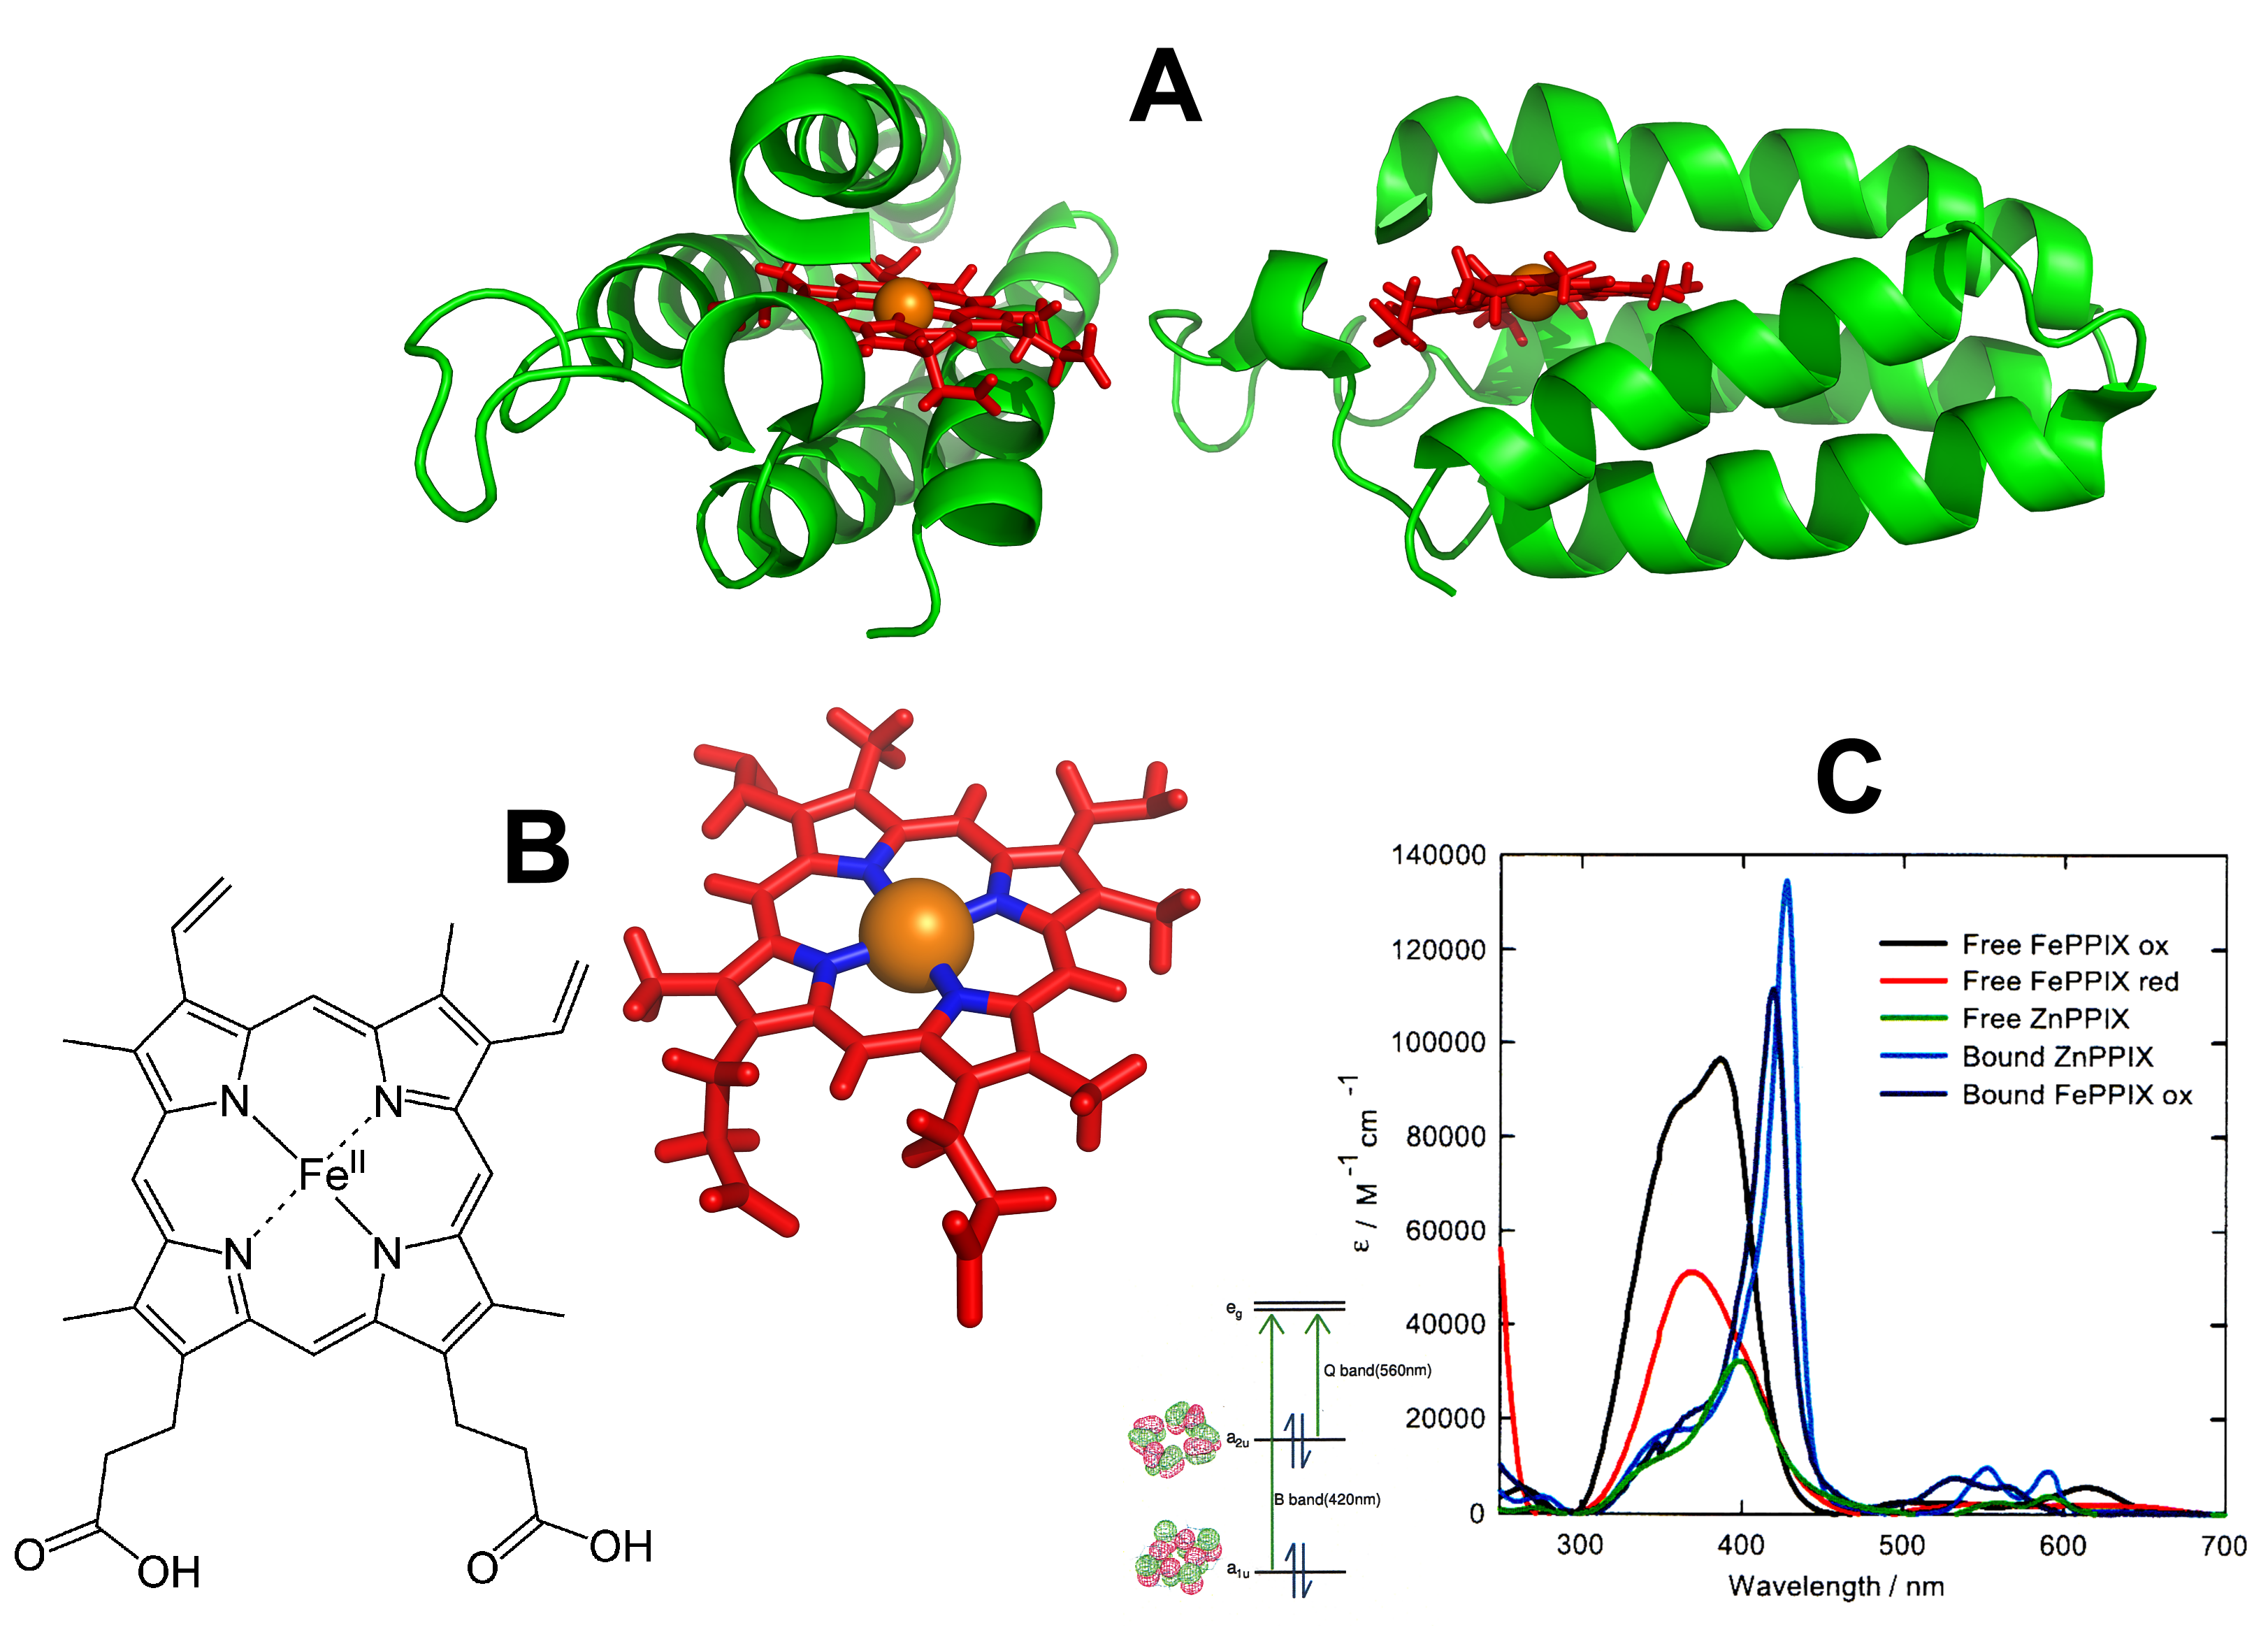
\includegraphics[width=137.4mm]{Images/haemStructure.png}
	\caption[Haem Structure]{A fancy image.}
	\label{fig:haemStructure}
\end{figure}
\end{verbatim}

\vspace{2ex}

\begin{figure}[!th]
	\centering
	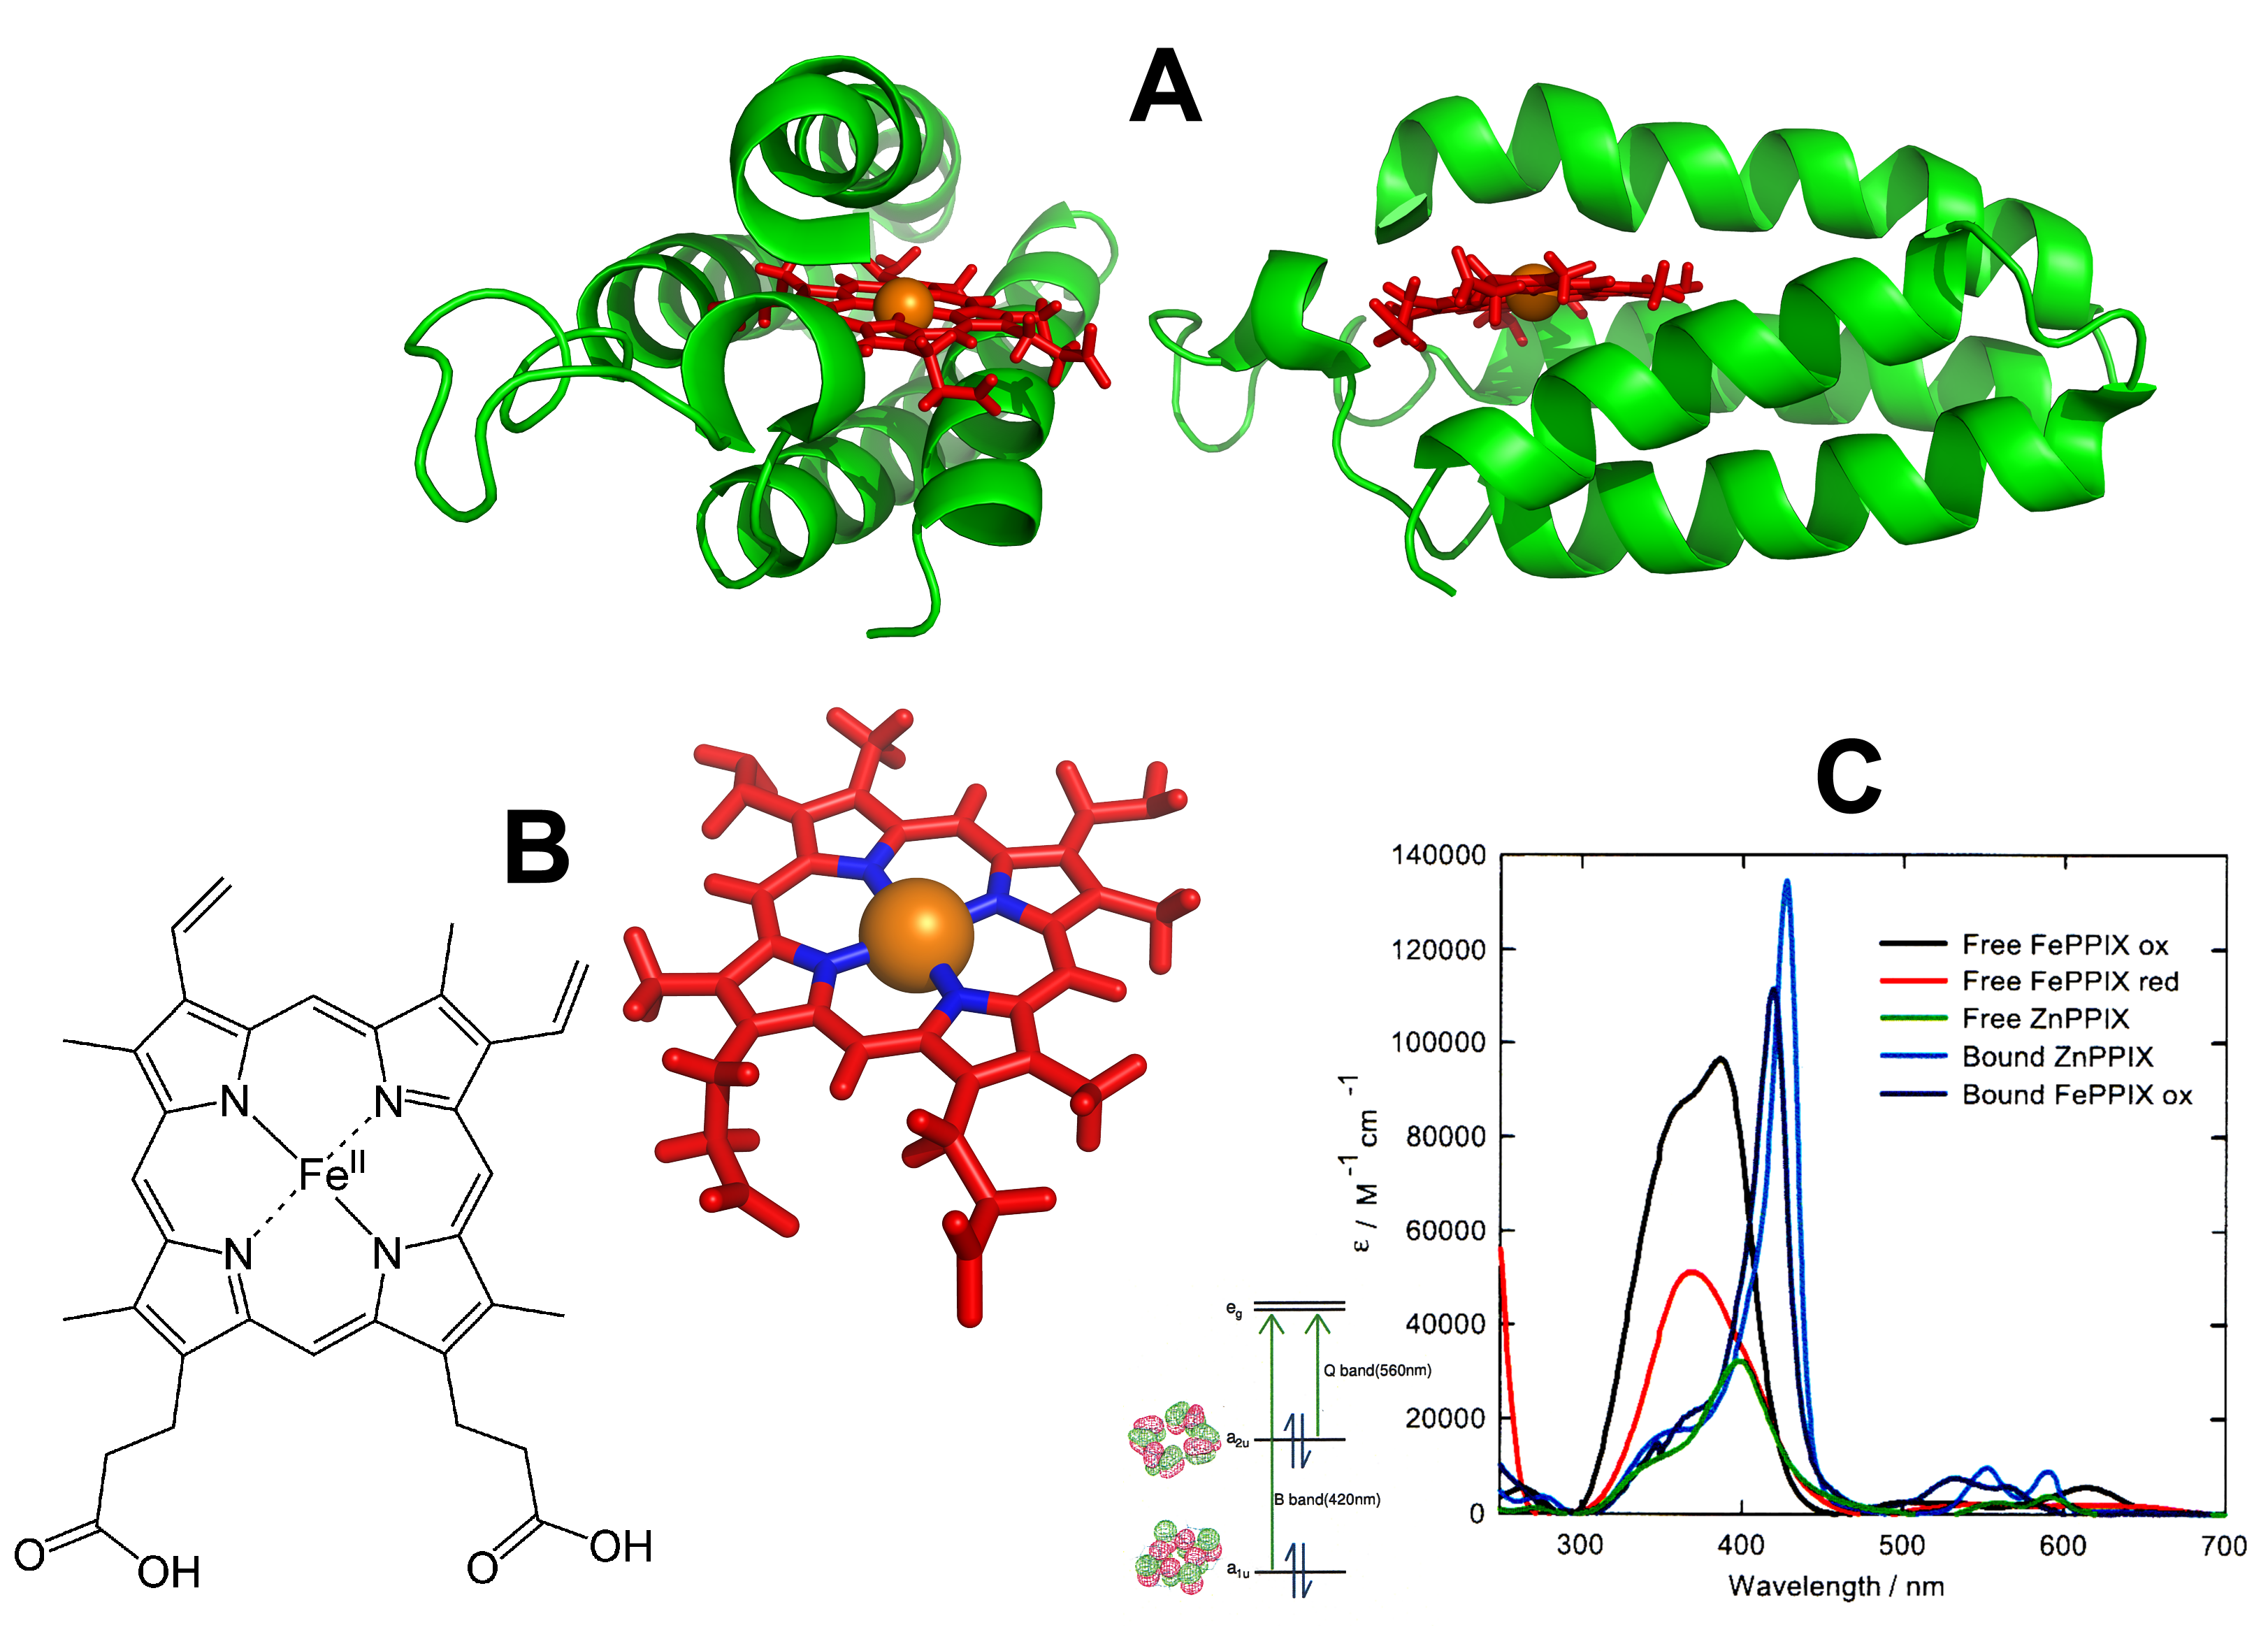
\includegraphics[width=137.4mm]{Images/haemStructure.png}
	\caption[Haem Structure]{A fancy image from Chris' Thesis.}
	\label{fig:haemStructure}
\end{figure}

In this example the command {\textbackslash}includegraphics tells LaTeX to look in the directory `Images' and incorporate the file called `haemStructure.png' into the final document while setting the width to 137.4mm.  This command can be used to resize a graphical file using the height or width parameter as shown. You must specify the units which can be pt, ex, em, mm, cm and so on. LaTeX recognises a very wide variety of standard units and graphics formats. The command is part of the graphicx package and so in the preamble you must include the command {\textbackslash}usepackage\{graphicx\}.

Many packages have been written to provide new commands. For example the `subfigure' package enables you to place separate images or files in the same figure side by side while giving them their own label. However, in this document we only concentrate on the very basics.

\section{Floating Environments}

Both tables and figures are examples of a `floating environments' which means LaTeX decides where to put them. 

The mysterious [!tbh] letters give guidance to LaTeX about roughly where the figure or table is  allowed to be, but in general they can move a long way from where you position them within your text file.  The letters in the square bracket can be t, h or b which stand for top, here or bottom.  If you don't specify any letters LaTeX defaults to [t].

LaTeX will always preserve the order in which figures appear.  If it cannot find a type setting solution, then it may move the float to it's own page, and combine it with other figures. If it still can't fit that in for some reason then it moves the float to the end of the document.  This has the effect of pushing all the remaining floating environments to the end of the document also.

The exclamation mark instructs LaTeX to ``try harder'' at putting the float where you told it to. Often you must play around to ensure the float positioning is acceptable, but usually this can be achieved by stretching or shrinking the image slightly using the size parameter, re-ordering text, judicial applications of the {\textbackslash}pagebreak command or by shouting loudly and slapping the computer monitor about. Note that it is better to resize the image using the original program that was used to create the image. Also using vector graphics can assist be useful (e.g. eps files) because they are designed to scale better.
\chapter{The Chapter on Making Chapters}
\label{sec:Chapters}

Right. LaTeX forces you to structure your document. There a series of simple commands for achieving this:

\vspace*{2ex}

{\textbackslash}chapter\{chapterName\}

{\textbackslash}section\{sectionName\}

{\textbackslash}subsection\{subsectionName\}

{\textbackslash}subsubsection\{subsubsectionName\}

\vspace*{2ex}

Easy enough. At the start of each chapter or section just issue one of these commands to name the section and LaTeX will present the chapter heading in the right style of font, which will be the same style of all the other heading names at that level of hierarchy throughout the document. In addition LaTeX assigns a number to that section. For example, this chapter was created using the command:

\vspace*{2ex}

{\textbackslash}chapter\{The Chapter on Making Chapters\} 

\vspace*{2ex}

LaTeX assigns the correct chapter number to each chapter in turn and then puts it in the table of contents, as you can see by looking at the table of contents! Easy.

\pagebreak
\section{The Section About Sections}
\label{sec:Section}
I think you're getting the hang of this. This section was created using the command {\textbackslash}section\{The Section About Sections\}. It appears in the table of contents as section \ref{sec:Section}.

\subsection{The Sub-Section About Sub-Sections}
\label{sec:SubSection}
Now you're really getting the hang of this. This subsection was created using the command {\textbackslash}subsection\{The Sub-Section About Sub-Sections\}. 

\subsubsection{The Sub-Sub-Section About Sub-Sub-Sections}
\label{sec:SubSubSection}
Now you're really getting the hang of this. but.. caught you out! This subsubsection doesn't have a number!  Ha Ha! It was created using the command {\textbackslash}subsubsection\{The Sub-Sub-Section About Sub-Sub-Sections\} in the same vein as all the other subsections/chapters etc. Here we have stopped the depth of the section numbering at the second level with the command:

\vspace*{2ex}

{\textbackslash}setcounter\{secnumdepth\}\{2\}

\vspace*{2ex}

Easy. WYSIWYM.  LaTeX does what you tell it to do. This is both a blessing and a curse.

\pagebreak
\section*{The Section About Sections That Don't Appear in the Table of Contents}
\label{sec:InvisibleSection}
Ok. Now we're throwing a spanner in the works. This section was created using the command:

\vspace*{2ex}

{\textbackslash}section*\{The Section About Sections That Don't Appear in the Table of Contents\}. 

\vspace*{2ex}

Notice how LaTeX has not assigned a number to the section and it doesn't appear in the table of contents. The effect of the * is to suppress the inclusion of a chapter, section or subsection in the automatic numbering. Easy. You can do this at any level. This is useful for things like prefaces, tables of contents or acknowledgements which you may or may not wish to have an entry in the main contents table. Up to you. It's your thesis. Don't just copy me.

\section{A Small Point About Numbering}

In this section notice how the numbering starts from where it left off before we suppressed the numbering on the previous section. Easy. WYSIWYM.
\pagebreak
\section{The Section About Internal Referencing}
\label{sec:InternalReferencing}

There are two related commands:

\vspace*{2ex}

{\textbackslash}label\{labelName\} 

{\textbackslash}ref\{labelName\}

\vspace*{2ex}


The {\textbackslash}label\{\} command allows you to create a label in a particular environment\footnote{That's right. Chapters, Sections and sub-sections etc are environments!}. The label won't appear in the final document. It's just a label which makes it easy to refer back to any particular environment elsewhere in the document. The {\textbackslash}ref\{\} command enables you to insert a reference anywhere in the document to any label in the document.  For example this is section \ref{sec:InternalReferencing}. The names you use in a label can be anything you like but musn't contain whitespace or special characters. I used the two commands:

\vspace*{2ex}

{\textbackslash}label\{sec:InternalReferencing\}

{\textbackslash}ref\{sec:InternalReferencing\}.

\vspace*{2ex}

The astute among you will realise that LaTeX has to read the document several times. Once to find the labels and then again to populate the references with the correct numbers. So you have to compile a latex document twice to get the referencing right. If there is a missing label or you refer to something that doesn't exist then latex inserts a convenient ? at that point. So hunting for queries is useful way of finding broken references. Latex issues warnings when it finds broken references.

As you create a document you will find yourself putting labels in all over the place so choose a sensible naming convention to help you remember the label names.

Each type of environment (equations, figures, tables, sections etc) has its own independent numbering system.  So when you choose your label name it's a good idea to have an identifier for that type of environment.  I have my own convention for label names which I use to help me remember references. E.g.   sec:SectionAboutCats. Eqn:EquationAboutCats,  Fig:FigureAboutCats and so on. This means you can differentiate between referring to the section or the figure more easily, even though they are about the same thing.

So Internal Referencing is a doddle. Easy!
\chapter{External Referencing}

Referencing is usually performed using a separate program called BibTex.  This program understands the file format .bib.

To create a reference within your document first you must create a .bib file by exporting your list of references from which ever referencing software you used, such as endnote, mendeley or whatever you use.

You can refer to an entry in the .bib file using the {\textbackslash}cite\{ref:Name\} command. the identifier `ref:Name' is the unique identifier which is the first line of each item included in your bibliography file.

For example, open the file LaTexCourseBib.bib in the bibliography directory. The first entry has the identifier `Horcas2007'.  This can be invoked as follows:


\begin{verbatim}
For example, this interesting fact\cite{Horcas2007}, is a cracking example.
\end{verbatim}

For example, this interesting fact\cite{Horcas2007}, is a cracking example.

During compilation latex and bibtex co-operate. During the first compilation latex generates a list of references that it needs.  During the second compilation bibtex populates the details from the .bib file into a shorter, ordered .bib file. The third compilation inserts markers at the right place in the main file and the fourth compilation generates the final list of references. Thus the compilation sequence is latex, bibtex, latex, latex.

The style of the referencing format can be changed using the command {\textbackslash}bibliographyStyle\{\}. e.g. the style used in this document is cjfthesisv1.bst which is invoked by 

\begin{verbatim}
\bibliographystyle{Bibliography/cjfthesisv1}
\end{verbatim}

The location of the list of references in the document is specified by issuing the {\textbackslash}bibliography\{\} command which also specifies the master bibliography file.

\begin{verbatim}
\bibliography{Bibliography/LaTeXCourseBib}
\end{verbatim}




\chapter{Organising Your Files}
One of the drawbacks of word is that the figures and tables are included within the document which becomes very very clunky quite quickly and once it reaches around 100Mb it becomes unwieldy and hard to export. One of that advantages of LaTeX is that the files are all text files and so are very light on resources and are easy to email around the place.

However, sometimes it can be difficult to navigate through a single text file, so if you had a huge document then it becomes difficult to find your way around.  One way of circumnavigating this problem is to break the file up into smaller files. As long as LaTeX knows where to look you can have a file for each logical sub-division of your document.

Therefore it is worth spending a bit of time at the beginning of a large project deciding how you wish to break up your LaTex Files and organise them neatly and tidily.  You can then tell LaTex where to look for the files using the following command:

\vspace*{2ex}
{\textbackslash}include\{fileName\}
\vspace*{2ex}

\pagebreak
\section{Linking a File}
We are now going to copy part of the tutorial file into a separate files and link it the main file.  Because this could go wrong it is sensible to back up tutorial.tex as something else. So save a copy called `tutorialOriginal.tex' for safe keeping. Then follow the following instructions.

\begin{enumerate}
\item Create a new file called MyFirstPage.tex
\item Select and Cut out the first chapter of Tutorial.Tex
\item Paste the first chapter into MyFirstPage.tex
\item Save both tutorial.tex and MyFirstPage.tex
\item Then add {\textbackslash}include\{MyFirstPage\} in tutorial.tex where the text used to be before you cut it out. We don't need to add the `.tex' because LaTeX can only include `.tex' files.
\item compile tutorial.tex and view the PDF
\end{enumerate}

The final PDF should look exactly the same as it was! except we now have a separate file for one of the chapters.

\pagebreak
\section{Creating A Class File}
We can also save our preamble in a separate file called a class file. This makes your main document much easier to understand.  To make it work we need to use the {\textbackslash}LoadClass\{\} command as follows: 

\begin{enumerate}
\item Create another new file and save it as TutorialStyle.cls
\item Copy the preamble of tutorial.tex into the new file. Starting with the {\textbackslash}documentclass{} command and copy right up to, but not including, the {\textbackslash}begin{document} command. Delete the preamble in the original document.
\item Save TutorialStyle.cls and tutorial.tex
\item Modify the first line of TutorialStyle.cls by replacing the word `document' with the word `Load'.
\item Add a new first line of tutorial.tex to use your new style class {\textbackslash}documentclass\{TutorialStyle\}
\item Save both files.
\end{enumerate}

\subsection{Sanity Check}

The first line of TutorialStyle.cls should now be:

\begin{verbatim}
\LoadClass[12pt, oneside, a4paper]{book}
\end{verbatim}
\vspace{2ex}

The first line of tutorial.tex should be:

\begin{verbatim}
\documentClass{TutorialStyle}
\end{verbatim}
\vspace{2ex}

We have just created what is called a style file. You can use this style file as a generic preamble for other documents as well. Compile tutorial.tex.  Nothing should have changed in the final PDF.


\pagebreak
\section{The Structure of this Document}

Lets now look at how I've organised this document. It is identical to my thesis because it started out life as my thesis. I usurped the structure and simply replaced the headings and content to make a kind of reference manual for this introductory course. This document therefore is three things:

\begin{enumerate}
\item An example thesis structure to work from.
\item The LaTeX files which were used to create it can be used as a template for a thesis.
\item It is also a convenient introductory latex manual!
\end{enumerate}

\vspace*{2ex}
Groovy huh?

\section{The Master File}

There is a master file where LaTeX begins the compilation procedure. This contains the {\textbackslash}documentclass command needed to set the ball rolling. Within the file there are a series of {\textbackslash}include\{\} commands, one for each Chapter, which tell LaTeX where to find the files containing each chapter.

The subfiles cannot be compiled on their own because they do not contain the {\textbackslash}documentclass, {\textbackslash}begin\{document\} or {\textbackslash}end\{document\} commands. Lets us look in more detail at the master file and we will learn some new LaTeX commands.

\singlespacing
\pagebreak
\begin{verbatim}
\documentclass{Style/LatexCourseStyle}

\begin{document}
\setcounter{secnumdepth}{2}
\setcounter{tocdepth}{1}

\frontmatter
\onehalfspacing
\include{Frontmatter/Titlepage}
\include{Frontmatter/Declaration}
\include{Frontmatter/Acknowledgements}
\include{Frontmatter/Summary}
\include{Frontmatter/Abbreviations}
\tableofcontents
\listoftables
\listoffigures

\mainmatter
\renewcommand{\sectionmark}[1]{\markright{\thesection \ #1}{}}
\include{Chapters/Overview}
\include{Chapters/MyFirstPage}
\include{Chapters/Lists}
\include{Chapters/mathsEquations}
\include{Chapters/ChemicalEquations}
\include{Chapters/Tables}
\include{Chapters/Figures}
\include{Chapters/Sectioning}
\include{Chapters/externalReferencing}
\include{Chapters/ThesisTemplateMainFile}
%\include{Chapters/ChapterThatIsNotCompiled}

\appendix
%\include{Appendices/UsefulWebsites}

\singlespacing

\backmatter
\addcontentsline{toc}{chapter}{References}
\bibliographystyle{Bibliography/cjfthesisv1}
\renewcommand{\bibname}{References}
\bibliography{Bibliography/LatexCourseBib}

\end{document}
\end{verbatim}
\onehalfspacing
\pagebreak

\section{Analysing the Master File}
Let us go through this file and observe the new commands. Most of it is self-explanatory.

\begin{verbatim}
\documentclass{Style/LaTeXCourseStyle}
\end{verbatim}

This command tells latex that the document class is the one defined in the the style file ''LaTeXCourseStyle'', which is in the sub directory ''style''.  Easy.

\begin{verbatim}
\setcounter{secnumdepth}{2}
\setcounter{tocdepth}{1}
\end{verbatim}

The first of these commands tells latex that the section depth number is 2. I.E. throughout the document only bother numbering sections, subsections and subsubsections down to the second level (such as section 1.2.3). The second command tells latex to only build the table of contents from section numbers down to the first level i.e. 1.1.  Easy enough.

The command {\textbackslash}frontmatter is exclusive to the book class, on which this style is based, and tells latex that within this section to number the pages using roman numerals, and not to include these numbers in the table of contents, just like in a book. The {\textbackslash}mainmatter and {\textbackslash}backmatter commands similarly delineate the other sections of the document.  

Childs play.  How long would it take you to figure out how to do that in word???? No idea. I've never tried.

Note that these rather cool commands are not available in every single class. So for a paper you would use the article class where such compartmentalisation of your document is not appropriate. In fact you can often download latex templates from the journal to wish to submit your paper, which is why I concentrate on the thesis template in this course.

\begin{verbatim}
\onehalfspacing
\end{verbatim}

Is obvious. ''From this point forward use line spacing of one and a half lines please. Thank you.'' How many hours have you spent clicking on paragraph indentations for each separate paragraphs in word? Nightmare. Want to change the standard in the whole document? Not a chance in word. In latex, you can do it with a single word, carefully placed in the master file.

\begin{verbatim}
\include{Frontmatter/Titlepage}
\include{Frontmatter/Declaration}
\include{Frontmatter/Acknowledgements}
\include{Frontmatter/Summary}
\include{Frontmatter/Abbreviations}
\end{verbatim}

The {\textbackslash}include\{\} command tells latex to include the specified .tex file at this point.  Thus it is a simple matter to break up a large document into sub components.  I have written each part of the front matter in a separate file and then grouped all the front matter into one directory called: Frontmatter.

See how the directory structure of my files reflects the structure of my book?

\begin{verbatim}
\tableofcontents
\listoftables
\listoffigures
\end{verbatim}

Again. This is easy. These commands mean: ''Please scan through the whole document and build for me a table of contents, a list of tables, a list of figures and then write down the entries along side their section numbers (as I have them ordered in this version of the document), as well as the page numbers on which they appear and create a nice little summary table and add them to the front matter of my document. Thanks.''.

How does latex do this?  remember the idea of environments?  Well each table, figure, equation etc is a defined environment.  LaTeX just counts them up and assigns numbers starting wherever you want and builds a table.  You can tell latex to ignore individual sections if you want to.

You can also control the look and feel of your table of contents with subtley and grace. Do you want to fill the white space with lines of dots to aid readability, even though the chapter titles are all different lengths? page numbers? How deep should the TOC been?  etc etc etc. How to do this is beyond the scope of this course, but now you know about it, go look it up. easy as $\pi$.

Ok.

Main matter we've done.

\begin{verbatim}
\renewcommand{\sectionmark}[1]{\markright{\thesection \ #1}{}}
\end{verbatim}

This command tells latex to 'renewcommand', i.e. change the meaning of the following command from this point in the document forward, over-riding previous definitions.
\begin{verbatim}
\sectionmark}[1]{\markright{\thesection \ #1}{}
\end{verbatim}

Is latex speak for ``please write the section heading at the top right hand side of each page. thanks''. This works in conjunction with a command in the style file which we'll talk about later. You have to tell latex to switch on headings as well as where to put them.

\begin{verbatim}
\include{Chapters/Overview}
\include{Chapters/MyFirstPage}
\include{Chapters/Lists}
\include{Chapters/mathsEquations}
\include{Chapters/ChemicalEquations}
\include{Chapters/Tables}
\include{Chapters/Figures}
\include{Chapters/Sectioning}
\include{Chapters/externalReferencing}
\include{Chapters/ThesisTemplateMainFile}
%\include{Chapters/ChapterThatIsNotCompiled}
\end{verbatim}

This is the include command again. You will notice that one of the include lines is commented out. This is a handy trick to only build certain parts of my thesis. Which can be useful if individual chapters are being reviewed.

\pagebreak

\begin{verbatim}
\appendix
%\include{Appendices/UsefulWebsites}

\singlespacing

\backmatter
\addcontentsline{toc}{chapter}{References}
\bibliographystyle{Bibliography/cjfthesisv1}
\renewcommand{\bibname}{References}
\bibliography{Bibliography/LatexCourseBib}
\end{verbatim}

The rest is easy. {\textbackslash}Appendix means we are in the appendix now and start labelling sections with A.1.2 instead of 1.2.3.  

{\textbackslash}addcontentsline means forcibly insert a contents line about the references into the contents table. 

{\textbackslash}\{bibliographystyle\{Bibliography/cjfthesisv1\}\} means use the biblography style defined in the file cjfthesisv1. Defining a bibliography style will be covered later if we have time. This is where you specify how the references will appear (names, journals, full stops, commas etc).

{\textbackslash}renewcommand\{{\textbackslash}bibname\}\{References\} means: rename the bibliography chapter as `References'

{\textbackslash}biblography means add the following bibliography.  You can reference entries in this bibliography file very easily.

The astute among you will realise that LaTeX will have to read the document several times before it can be compiled with all the references.  Hey ho. No problem. You can go and have a cuppa while LaTeX does your references for you in the style of your favorite journal... nice.




%\include{Chapters/ChapterThatIsNotCompiled}

\appendix
%\include{Appendices/UsefulWebsites}

\singlespacing

\backmatter
\addcontentsline{toc}{chapter}{References}
\bibliographystyle{Bibliography/cjfthesisv1}
\renewcommand{\bibname}{References}
\bibliography{Bibliography/LatexCourseBib}

\end{document}
\end{verbatim}
\onehalfspacing
\pagebreak

\section{Analysing the Master File}
Let us go through this file and observe the new commands. Most of it is self-explanatory.

\begin{verbatim}
\documentclass{Style/LaTeXCourseStyle}
\end{verbatim}

This command tells latex that the document class is the one defined in the the style file ''LaTeXCourseStyle'', which is in the sub directory ''style''.  Easy.

\begin{verbatim}
\setcounter{secnumdepth}{2}
\setcounter{tocdepth}{1}
\end{verbatim}

The first of these commands tells latex that the section depth number is 2. I.E. throughout the document only bother numbering sections, subsections and subsubsections down to the second level (such as section 1.2.3). The second command tells latex to only build the table of contents from section numbers down to the first level i.e. 1.1.  Easy enough.

The command {\textbackslash}frontmatter is exclusive to the book class, on which this style is based, and tells latex that within this section to number the pages using roman numerals, and not to include these numbers in the table of contents, just like in a book. The {\textbackslash}mainmatter and {\textbackslash}backmatter commands similarly delineate the other sections of the document.  

Childs play.  How long would it take you to figure out how to do that in word???? No idea. I've never tried.

Note that these rather cool commands are not available in every single class. So for a paper you would use the article class where such compartmentalisation of your document is not appropriate. In fact you can often download latex templates from the journal to wish to submit your paper, which is why I concentrate on the thesis template in this course.

\begin{verbatim}
\onehalfspacing
\end{verbatim}

Is obvious. ''From this point forward use line spacing of one and a half lines please. Thank you.'' How many hours have you spent clicking on paragraph indentations for each separate paragraphs in word? Nightmare. Want to change the standard in the whole document? Not a chance in word. In latex, you can do it with a single word, carefully placed in the master file.

\begin{verbatim}
\thispagestyle{empty}

\begin{center}
\vspace*{\stretch{1}}

\hrule height 2pt
\vspace*{2ex}
{\Huge\textbf{Towards the Ability to Make Super Duper LaTeX Documents}\par}
\vspace*{2ex}
\hrule height 2pt
\vspace*{10ex}
{
\includegraphics[height=40mm]{Images/UnivShield}\par}
\vspace*{10ex}
{\large\textbf{Christopher~James~Forman}\par}
\vspace*{2ex}
{\large{Department Of Chemistry}\par}
\vspace*{2ex}
{\large{University of Cambridge}\par}
\vspace*{5ex}
{\large{This dissertation is submitted for the degree of \textit{Doctor of Philosophy}}\par}
\vspace*{5ex}
{\large{\today}\par}

\vspace*{\stretch{2}}
\end{center}
\chapter*{Declaration}

\vfill

This dissertation is the result of my own work and includes nothing which is the outcome of work done in collaboration except where specifically indicated in the text. It is not substantially the same as any that I have submitted for a degree or diploma or other qualification at any other University and no part has already been, or is concurrently being, submitted for any degree, diploma, or other qualification. It does not exceed 60,000 words, including tables, footnotes, bibliography and appendices.\par

\vspace{10ex}

\begin{flushright}
Signature: \rule[0pt]{60mm}{0.5pt}

\vspace{5ex}

Date: \rule[0pt]{60mm}{0.5pt}
\end{flushright}

\vfill
\chapter*{Acknowledgments}
\subsection*{Family}
Mum. Dad. Pet Dog.

\subsection*{Scientific Collaborations}
Dr A.N.Other at uni of blah for samples and instrument time etc. My Amazing Lab Chums.

\subsection*{Scientific Support}
My amazing lab chums.

\subsection*{General Assistance}
Cleaner, My amazing lab chums.

\subsection*{Financial Support}
Bank, Tax payer. My amazing lab chums.

\subsection*{Moral Support}
My Amazing Lab chums.

\subsection*{Academic Inspiration}
Netwon, My super. My Amazing Lab Chums.

\subsection*{Everyone else}
My Amazing Lab Chums.

\chapter*{Summary}
This document is a handbook for introducing you to LaTeX. It contains a bit of background about the history and philosophy of LaTeX.  However, it concentrates on providing a guided practical introduction to the basic techniques such as 
\begin{itemize}
\item Lists
\item Mathematical and chemical equations
\item Tables
\item Figures
\item Chapters and Sections
\item Linking to other files in large documents
\item Referencing
\end{itemize}

The handbook is also presented in the style of a thesis. This means that source files provided on the introductory course and available from the department web page are a convenient template for a thesis.

More details on specific aspects of LaTeX can be found at the departmental LaTeX page which can be found here:

 http://www-ch-int.ch.private.cam.ac.uk/latex/about

\chapter*{Abbreviations}

\begin{longtable}{r >{\rule{0pt}{3ex}}l<{\rule[-1.5ex]{0pt}{0pt}}}
ADP & Adenosine Diphosphate\\
(nc/c)AFM & (non-contact/conducting) Atomic Force Microscopy\\
ATP & Adenosine Triphosphate \\
\end{longtable}
\end{verbatim}

The {\textbackslash}include\{\} command tells latex to include the specified .tex file at this point.  Thus it is a simple matter to break up a large document into sub components.  I have written each part of the front matter in a separate file and then grouped all the front matter into one directory called: Frontmatter.

See how the directory structure of my files reflects the structure of my book?

\begin{verbatim}
\tableofcontents
\listoftables
\listoffigures
\end{verbatim}

Again. This is easy. These commands mean: ''Please scan through the whole document and build for me a table of contents, a list of tables, a list of figures and then write down the entries along side their section numbers (as I have them ordered in this version of the document), as well as the page numbers on which they appear and create a nice little summary table and add them to the front matter of my document. Thanks.''.

How does latex do this?  remember the idea of environments?  Well each table, figure, equation etc is a defined environment.  LaTeX just counts them up and assigns numbers starting wherever you want and builds a table.  You can tell latex to ignore individual sections if you want to.

You can also control the look and feel of your table of contents with subtley and grace. Do you want to fill the white space with lines of dots to aid readability, even though the chapter titles are all different lengths? page numbers? How deep should the TOC been?  etc etc etc. How to do this is beyond the scope of this course, but now you know about it, go look it up. easy as $\pi$.

Ok.

Main matter we've done.

\begin{verbatim}
\renewcommand{\sectionmark}[1]{\markright{\thesection \ #1}{}}
\end{verbatim}

This command tells latex to 'renewcommand', i.e. change the meaning of the following command from this point in the document forward, over-riding previous definitions.
\begin{verbatim}
\sectionmark}[1]{\markright{\thesection \ #1}{}
\end{verbatim}

Is latex speak for ``please write the section heading at the top right hand side of each page. thanks''. This works in conjunction with a command in the style file which we'll talk about later. You have to tell latex to switch on headings as well as where to put them.

\begin{verbatim}
\chapter{Overview}
\label{chap:overview}
\section{LaTeX: The answer to everything.}
LaTeX is typsetting program that takes an input file of marked up text and then, with a user defined set of rules, typesets a beautifully crafted output file that can be easily printed (e.g. a pdf). 

\subsection{Advantages}

The advantages of this method are manifold:

\begin{itemize}

\item Use any text editor to view the source document.
\item More time can be spent working on the content and not worrying about how text or figures interact in the layout until later on.
\item LaTeX uses consistent rules throughout a document
\item LaTeX sorts out basic typesetting automatically
\item Changes can be introduced globally with very little effort
\item Document structure is explicit
\item Documents can be professionally typeset and look great
\item You are forced to structure your documents correctly.
\item Mathematical equations, like $E=mc^2$ or $\imath\hbar\frac{\partial}{\partial t}\Phi (x, t) = \hat{H}\Phi (x, t)$ can be produced almost as fast as typing (if you know the commands!).
\end{itemize}

\subsection{Disadvantages}
The disadvanatges of this method are also manifold:
\begin{itemize}
\item You don't see the output as you go.
\item Steep learning curve.
\item Documents are harder to edit by a second author (unless they are adept at LaTeX too). This can be mitigated using version control, which makes group authoring processes superior to word.
\item The program never works quite the way you want it to and learning how to influence it can be problematic and subtle.
\item Although intended to save work the principle of 'conservation of work' means that you simply transform problems associated with WYSISYG approaches to problems associated with WYSIWYM approaches!
\item You can go blind trying to determine the difference between wiggly and smooth brackets if your editors font isn't large enough.
\end{itemize}

\subsection{On balance?}
If it's so rubbish, why use LaTeX?

\begin{itemize}
\item Large documents are much more easily handled. 
\item In general it is quicker to debug a LaTeX document than typeset an entire thesis manually. 
\item Technical information such as tables, equations and figures are integrated much more smoothly than with word.
\end{itemize}

\section{How does it work?}

The raw text is interspersed with commands, preceded by a \textbackslash, which tell LaTeX what to do with the text. For example you can \textbf{make it bold}, \emph{italic}, or \underline{underlined} with the commands {\textbackslash}textbf\{\}, {\textbackslash}emph\{\} or {\textbackslash}underlined\{\}. More on commands in a moment...



\chapter{My First Page}

\section{The Very Beginning}
The very simplest LaTeX document might look like this:

\begin{verbatim}
\documentclass[a4paper,12pt]{article}
\begin{document}
Hello World.
\end{document}
\end{verbatim}

\pagebreak
\thispagestyle{empty}
Hello World.
\pagebreak
\subsection{Break Down}
What's all the gobbledegook around my simple message???

In LaTeX we intersperse text and commands.  Commands are preceded by a \textbackslash. For example the first line in a LaTeX document \underline{\textbf{\emph{must}}} be:

\begin{verbatim}
\documentclass[options]{class}
\end{verbatim}

Where the word ''class'' may be substituted for one of many things such as: article, proc, minimal, report, book, letter, memoir, slides, beamer.

Similarly, and completely generally in LaTeX speak, the square brackets denote the existence of optional parameters. Each individual command can take its own parameters and for the ''{\textbackslash}documentclass'' command there are options for controlling font size, font family, landscape, oneside, twosided, page size and so on. These options will persist throughout the entire document. For example the document class command for this document, (which is likely to be like the one you would use for a thesis), would be:

\begin{verbatim}
\documentclass[12pt, oneside, a4paper]{book}
\end{verbatim}

Other options include:

\begin{itemize}
\item {10pt, 11pt, 12pt (default is 10pt).}
\item {letterpaper, legalpaper, a4paper, executivepaper, a5paper, b5paper}
\end{itemize}
and so on.

\pagebreak
\section{Can I start typing please?}

After we have set up the document we can start actual work on our document. So we must tell LaTeX that what follows is to be interpreted as a document.  The command {\textbackslash}begin can take many different parameters and is a command to enter what is known, in LaTeX speak, as 'an environment'. Thus the commands:
\begin{verbatim}
\begin{document}

\end{document}
\end{verbatim}

tells LaTeX to enter and leave the document environment, and thus constitute the outer limits of our document file. Other environments include the equation environment, the itemize environment, the figure environment and so on. These will be encountered in due course.

Every part of the LaTeX file is therefore within an environment of specific type and the content within each environment consists of commands or text.

That's basically it.

So let's get on with it shall we...

\pagebreak
\section{The ground rules}
\begin{quote}
Hold on, hold on, hold on my son.

First the lessons.

Then the fun!
\end{quote}
Dr Seuss.

\subsection{Spaces}
Whitespace characters, such as blank or tab, are treated uniformly as space by LaTeX. Several consecutive whitespace characters are treated as one single space. Whitespace at the start of a line is generally ignored, and a single line break is treated as whitespace. An empty line between two lines of text defines the end of a paragraph. Several empty lines are treated the same as one empty line. The text below is an example.

\begin{verbatim}
It does not matter whether you
enter one or several             spaces
after a word. The final result will be typeset beautifully
according    to     precise rules.




An empty line starts a new
paragraph. Note the indentation on the first line of the paragraph, 
except at the beginning of the section. 
\end{verbatim}

\vspace*{2ex}
\vspace*{2ex}

It does not matter whether you
enter one or several             spaces
after a word. The final result will be typeset beautifully
according    to     specific rules.




An empty line starts a new
paragraph. Note the indentation on the first line of the paragraph, except at the beginning of the section. 

\pagebreak
\subsection{Special Characters}
The symbols 

\# \$ \% \textasciicircum{} \& \_ \{ \} \~{} \textbackslash

are reserved characters that either have a special meaning under LaTeX or are unavailable in all the fonts. If you enter them directly in your text, they will normally not print, but rather make LaTeX do strange things.

To overide the special meanings of these symbols and allow them to produced within your text you may use the following sequences:
\begin{verbatim}
\# \$ \% \textasciicircum{} \& \_ \{ \} \~{} \textbackslash
\end{verbatim}

Other symbols and many more can be printed with special commands in mathematical formulae or as accents.

The backslash character '\textbackslash' cannot be entered by adding another backslash in front of it ( \textbackslash\textbackslash); because this sequence means ''linebreak''.

The command \textbackslash\~{}\{\} produces a tilde which is placed over the next letter. For example \textbackslash\~{}\{n\} gives \~{n}. To produce just the character \~{}, use \textbackslash\~{}\{\} which places a \~{} over an empty box.

Similarly, the command \textbackslash\textasciicircum{} produces a hat over the next character, for example \textbackslash\textasciicircum\{o\} produces \^{o}.

\pagebreak
\section{Preamble}
After the {\textbackslash}documentclass command we add ''preamble''. Here we load special features that we will use throughout our document to expand on the basic capabilities of LaTex. These are contained in units called ''packages'' which we can tell our LaTeX compiler to download by using the command ''{\textbackslash}include\{packageName\}''. 

There are many repositories of such packages on the web. Your compiler generally knows where to look and most standard packages are included with any install. For example, to include a special set of typesetting instructions to handle chemical equations we can grow our simple document with a single command like this:

\begin{verbatim}
\documentclass[a4paper,12pt]{article}
\usepackage[version=3]{mhchem}
\begin{document}
Hello World!

We all need \ce{H2O}.

I'm less fussed about \ce{^{235}_{92}U+}.

\end{document}
\end{verbatim}

\vspace{2ex}

\pagebreak
\thispagestyle{empty}
Hello World!

We all need \ce{H2O}.

I'm less fussed about \ce{^{235}_{92}U+}.
\pagebreak

Here we have loaded a package called: "`mhchem"' which took the option ''[version=3]''. This is a package for drawing chemical equations easily and it has it's own instruction manual which you can follow easily. It is included in the bundle of files for this course.

Other things we can do in the premable within LaTeX are to redefine existing commands or create our own personal commands. These can be stored in a file called the 'style file' which we can load at the beginning of our document, in place of our documentclass. More about this later on...


\subsection{Comments}
It is often useful to comment your LaTeX documents. You can leave yourself amusing, sarcastic messages that won't get printed out in the final document. Use this to make your own notes as the course progresses.

To get a comment use the \% command, which tells LaTeX to ignore the rest of the line, the line break and all the white space at the beginning of the next line, for example, we may add to our continually evolving document...

\begin{verbatim}
\documentclass[a4paper,12pt]{article}
\usepackage[version=3]{mhchem}
\begin{document}
Hello World!

%All humans need water and I would like 
%to include this concept in my arguments.
We all need \ce{H2O}.

%Uranium 235 is toxic, which is why I don't want to consume it... 
I'm less fussed about \ce{^{235}_{92}U+}.

\end{document}
\end{verbatim}

\vspace{4ex}
Hello World!

%All humans need water and I would like to include this concept in my arguments.
We all need \ce{H2O}.

%Uranium 235 is toxic, which is why I don't want to consume it... 
I'm less fussed about \ce{^{235}_{92}U+}.

\pagebreak
\section{Compiling}
Once the document is finished you can compile it. Your compiler will depend on the platform that you use. In the PWF we are using winEDT to edit the documents (a LaTeX front end) and texlive2008 which is the compiler itself. I use MiKTex and the front end texCenter.  There is no need to use a front end. If you prefer you can use a simple text editor and a command line.

the recommended distributions are:
\begin{itemize}
\item MiKTeX or TeX Live for Windows
\item TeX Live for Unix/Linux
\item MacTeX or TeX Live for Mac OS.
\end{itemize}

Once you have installed your software and got it working, written your source code and tried to compile it, there will nearly always be something wrong with your file. 

Any errors will be highlighted in the console window or error output box of your front end.  Some front ends dump the running commentary which LaTeX produces into a text file for easy reading afterwards.

In a compile attempt (successful or otherwise) LaTeX may produce the following files:

projectname.aux

projectname.bbl

projectname.lof

projectname.lot

projectname.txt

projectname.toc

projectname.dvi

These are interim files (toc= table of contents, bbl = bibliography etc). To be honest I have no idea what half of these things contain.  You only need the .tex file and a compiler with the right packages installed to produce them again.

Some versions of LaTeX only produce DVI files and you then need to convert the dvi file to a PDF or download a dvi viewer. You can also convert DVI files to PS files and then view them.  The good thing about front ends is that you can set them up to produce PDFs directly.

OK. So we have now produced a silly document but we understand it.  Now lets get on with learning how to make our own documents.



\chapter{Lists}
Lists are great.  The command {\textbackslash}begin\{\} can be used to enter a list environment.  For example:

\begin{verbatim}
\begin{itemize}
\item cat
\item dog
\item horse
\end{itemize}
\end{verbatim}

Produces:

\begin{itemize}
\item cat
\item dog
\item horse
\end{itemize}

\pagebreak
We can also replace the bullet points with numbers using the enumerate keyword.

\begin{verbatim}
\begin{enumerate}
\item cat
\item dog
\item horse
\end{enumerate}
\end{verbatim}

\begin{enumerate}
\item cat
\item dog
\item horse
\end{enumerate}

\pagebreak
and we can use the description keyword which does this:
\begin{verbatim}
\begin{description}
\item[Cat] a lovely furry creature with a cute nose and whiskers.
\item[Dog] Another furry creature that smells rather well; 
           its olfactory power stems from its nasal dampness.
\item [Horse] A large stinky creature with sideways facing eyes.
\end{description}
\end{verbatim}

\begin{description}
\item[Cat] a lovely furry creature with a cute nose and whiskers.
\item[Dog] Another furry creature that smells rather well; its olfactory power stems from its nasal dampness.
\item [Horse] A large stinky creature with sideways facing eyes.
\end{description}
\chapter{Maths Equations}

\section{Producing Beautiful Looking Mathematics}

One of the best features about LaTeX is `maths mode'.  For example the schrodinger equation can be produced as follows:

\vspace*{2ex}

\begin{center}
\begin{math}
\imath\hbar\frac{\partial}{\partial t}\Phi (x, t) = \hat{H}\Phi (x, t)
\end{math}
\end{center}

\vspace*{2ex}

\begin{verbatim}
\begin{math}
\imath\hbar\frac{\partial}{\partial t}\Phi(x,t)=\hat{H}\Phi(x,t)
\end{math}
\end{verbatim}

There are a number of ways to switch on maths mode.  The first, as above, is with the {\textbackslash}begin\{math\} environment. You can also enter mathmode inline using the \$ symbol. For example typing in \$y=ax\textasciicircum{}2+bx+c\$ yields $y=ax^2+bx+c$.  Another way is to enter the equation environment which enables you to number equations so you can then refer to them later in the text.

\begin{equation}
y(t)= \sin \left(\frac{{\alpha}t}{2\pi} + \phi_0\right)
\label{eqn:MadeUpNonsense}
\end{equation}

\vspace*{2ex}
\begin{verbatim}
\begin{equation}
y(t)= \sin \left(\frac{{\alpha}t}{2\pi} + \phi_0\right)
\end{equation}
\end{verbatim}.

\section{Basic Maths Mode}
Once in maths mode there is a kind of text based code for writing down your equations.  Here are the most basic symbols to get you going.
\begin{center}
\begin{tabular}{cc}
\toprule
Final Result & LaTeX Code \\
\cmidrule(){1-2}
$a+b$ & a+b \\
$a-b$ & a-b \\
$ab$ & ab \\
$a*b$ & a*b \\
$a \times b$ & a {\textbackslash}times b \\
$a \cdot b$ & a {\textbackslash}cdot b \\
$\frac{a}{b}$ & {\textbackslash}frac\{a\}\{b\} \\ 
$a^b$ & a\textasciicircum{}b \\
$a_b$ & a\_b \\
$\sin a$ & {\textbackslash}sin a  (same for cos, tan)\\
$ sin a$ & sin a \\
$\sqrt{a}$ & {\textbackslash}sqrt\{a\} \\
$\left( a \right) $ & {\textbackslash}left( a {\textbackslash}right)\\ 
$\left[ a \right]$ & {\textbackslash}left[ a {\textbackslash}right]\\ 
$\alpha$ & {\textbackslash}alpha \\
$\pi$ & {\textbackslash}pi \\
\bottomrule
\end{tabular}
\end{center}

A full treatise on maths mode is not practical here. There are lots of online tutorials and summaries of symbols. It just takes a bit of practice and you can build up equations really easily. It's straight forward to learn new stuff once you've done it a few times.

\pagebreak
\section{Equation Arrays}
Sometimes you need to arrange several equations vertically, referencing individual lines separately and aligning the equations on the $=$ sign. This can be achieved with equation arrays as follows:

\begin{eqnarray}
A\left( x\right) & = & \frac{x^2+2x+1}{x+1} \\
& = & \frac{\left(x+1\right)\left(x+1\right)}{x+1} \nonumber\\
& = & x+1 \nonumber\\
B(x,t) & = & \frac{e^{\left(\imath\omega_0 t + kx\right)}}{4\pi\epsilon_0}
\end{eqnarray}

\begin{verbatim}
\begin{eqnarray}
A\left( x\right) & = & \frac{x^2+2x+1}{1+x} \\
& = & \frac{\left(x+1\right)\left(x+1\right)}{1+x} \nonumber\\
& = & x+1 \nonumber\\
B(x,t) & = & \frac{e^{\left(\imath\omega_0 t + kx\right)}}{4\pi\epsilon_0}
\end{eqnarray}
\end{verbatim}

\begin{itemize}
\item Note the \& symbols. This tells LaTeX where to align the equations. There must be the same number of \& symbols in each line.
\item Note the \textbackslash\textbackslash ~at the end of each line except the last one. This symbol tells LaTeX to add another row in the array.  If you put it on the last line you get an empty row at the bottom of the array.
\item Note the {\textbackslash}nonumber command which suppresses line numbering for that line.
\item Note that equation number carries on from equation \ref{eqn:MadeUpNonsense} in the previous section.
\end{itemize}

\section{Maths Packages}

Maths mode comes as standard in LaTeX, however you can download packages that buff up your maths symbol set. For example neat vector notation comes in the package `vector'. e.g. {\textbackslash}uuvec\{T\} yields $\uuvec{T}$.

\begin{verbatim}
\usepackage{amssymb}
\usepackage{amsmath}
\usepackage{vector}
\end{verbatim}


\chapter{Chemical Equations}
The mhchem package means you can do basic stuff very easily using {\textbackslash}ce\{\}. For example:

\vspace{2ex}
\begin{verbatim}
\ce{CO2 + C -> 2CO}
\ce{CO2 + C <- 2CO}
\ce{CO2 + C <=> 2CO}
\ce{A-B=C#D\sbond E\dbond F\tbond G}
\end{verbatim}
\vspace{2ex}
\begin{center}
\ce{CO2 + C -> 2CO}

\ce{CO2 + C <- 2CO}

\ce{CO2 + C <=> 2CO}

\ce{A-B=C#D\sbond E\dbond F\tbond G}
\end{center}

\vspace{2ex}
You can also use math mode within chemical equations.
\vspace{2ex}

\begin{center}
\ce{$x\,$ Na(NH4)HPO4 ->[\Delta] (NaPO3)_{$x$} + $x\,$ NH3 ^ + $x\,$ H2O}
\end{center}

\begin{verbatim}
\ce{$x\,$ Na(NH4)HPO4 ->[\Delta](NaPO3)_{$x$} + $x\,$ NH3 ^ + $x\,$ H2O}
\end{verbatim}

And you can number chemical reactions as well by using the math mode equation environment.

\begin{equation}
\ce{CO2 + C <=> 2CO}
\end{equation}

\begin{verbatim}
\begin{equation}
\ce{CO2 + C <=> 2CO}
\end{equation}
\end{verbatim}

However, this will number mathematical and chemical equations using the same number system. There is a discussion in the mhchem pdf which shows you how to number chemical and mathematical equations independently. It's a bit complex and involves you creating your own type of environment... bit beyond the intro level of this course...
\chapter{Tables}
Tables are big business in Latex.  I use these packages to help me.

\begin{verbatim}
\usepackage{multirow}
\usepackage{booktabs}
\usepackage{dcolumn}
\end{verbatim}

Here's an example table

\begin{table}[!hb]
 \centering
	\begin{tabular}{@{}rccc@{~}r@{.}l*3{r@{.}l@{~}r@{.}l}D{.}{\cdot}{2,1}}
	\toprule
	\multicolumn{1}{c}{Fibre Type}
	& N 
	& M 
	&\multicolumn{3}{c}{$L_t$ (nm)}
	&\multicolumn{4}{c}{$R_t$ (nm)}
	&\multicolumn{4}{c}{$d_t$ (nm)}
	&\multicolumn{4}{c}{${\Delta}Z_t$ (nm)}
	&\multicolumn{1}{c}{~}\\
\cmidrule(lr){1-1}
\cmidrule(lr){2-2}
\cmidrule(lr){3-3}
\cmidrule(lr){4-6}
\cmidrule(lr){7-10}
\cmidrule(lr){11-14}
\cmidrule(lr){15-18}
  SS Twisted & 5 & 4 & 313 &\multicolumn{2}{c}{(122)} & 5&7 &(1&6)  & 5&4 &(1&0)  &  150&5 &(63&1) &\multicolumn{1}{c}{~} \\
  \multicolumn{19}{c}{~}\\
  %\cmidrule(lr){3-18}
  &
  &
 	&\multicolumn{3}{c}{$L_s$ (nm)} 
 	&\multicolumn{4}{c}{$R_s$ (nm)}
 	&\multicolumn{4}{c}{$W_s$ (nm)}
 	&\multicolumn{4}{c}{${\Delta}Z_s$ (nm)}
 	&\multicolumn{1}{c}{${\Delta}Z_{e}$ (nm)}\\
\cmidrule(lr){4-6}
\cmidrule(lr){7-10}
\cmidrule(lr){11-14}
\cmidrule(lr){15-18}
\cmidrule(lr){19-19}
  SS Spiral& 32 & 7 &123&(31&6)&11&4&(3&3)&11&1&(2&6)&32&9&(22&2)&26.9\\
  SSB Spiral& 64&18 &106&(22&9)&10&8&(2&7)&9&8&(1&8)&28&2&(8&1)&22.7\\
	%\midrule
  BSS Spiral&37 &19 &110&(44&9)&13&4&(3&0)&12&9&(1&8)&27&1&(9&1)&21.5\\
	%\midrule
  SSSB Spiral&26& 6 &104&(23&9)&13&3&(2&6)&16&4&(3&4)&29&9&(11&1)&22.5\\
	\bottomrule
	\end{tabular}	
	\caption[Basic Fibre Dimensions by TEM]{A funky table from my thesis.}
	\label{tab:BasicXSBFibreDimensionsTEM}
\end{table}

\pagebreak
Here's what the code looks like:
\begin{verbatim}
\begin{table}[!hb]
 \centering
	\begin{tabular}{@{}rccc@{~}r@{.}l*3{r@{.}l@{~}r@{.}l}D{.}{\cdot}{2,1}}
	\toprule
	\multicolumn{1}{c}{Fibre Type}
	& N 
	& M 
	&\multicolumn{3}{c}{$L_t$ (nm)}
	&\multicolumn{4}{c}{$R_t$ (nm)}
	&\multicolumn{4}{c}{$d_t$ (nm)}
	&\multicolumn{4}{c}{${\Delta}Z_t$ (nm)}
	&\multicolumn{1}{c}{~}\\
\cmidrule(lr){1-1}
\cmidrule(lr){2-2}
\cmidrule(lr){3-3}
\cmidrule(lr){4-6}
\cmidrule(lr){7-10}
\cmidrule(lr){11-14}
\cmidrule(lr){15-18}
  SS Twisted & 5 & 4 & 313 &\multicolumn{2}{c}{(122)} & 5&7 &(1&6)  & 5&4 &(1&0)  &  150&5 &(63&1) &\multicolumn{1}{c}{~} \\
  \multicolumn{19}{c}{~}\\
  %\cmidrule(lr){3-18}
  &
  &
 	&\multicolumn{3}{c}{$L_s$ (nm)} 
 	&\multicolumn{4}{c}{$R_s$ (nm)}
 	&\multicolumn{4}{c}{$W_s$ (nm)}
 	&\multicolumn{4}{c}{${\Delta}Z_s$ (nm)}
 	&\multicolumn{1}{c}{${\Delta}Z_{e}$ (nm)}\\
\cmidrule(lr){4-6}
\cmidrule(lr){7-10}
\cmidrule(lr){11-14}
\cmidrule(lr){15-18}
\cmidrule(lr){19-19}
  SS Spiral& 32 & 7 &123&(31&6)&11&4&(3&3)&11&1&(2&6)&32&9&(22&2)&26.9\\
  SSB Spiral& 64&18 &106&(22&9)&10&8&(2&7)&9&8&(1&8)&28&2&(8&1)&22.7\\
	%\midrule
  BSS Spiral&37 &19 &110&(44&9)&13&4&(3&0)&12&9&(1&8)&27&1&(9&1)&21.5\\
	%\midrule
  SSSB Spiral&26& 6 &104&(23&9)&13&3&(2&6)&16&4&(3&4)&29&9&(11&1)&22.5\\
	\bottomrule
	\end{tabular}	
	\caption[Basic Fibre Dimensions by TEM]{A funky table from my thesis.}
	\label{tab:BasicXSBFibreDimensionsTEM}
\end{table}
\end{verbatim}

\pagebreak

\section{Tables Made Easy}
Here is a simple table followed by the code that produced it.

\begin{center}
\begin{tabular}{lcr}
anchovy & banana & carrot \\
dog & apple & fennel \\
goat & strawberry & potato
\end{tabular}

\vspace*{2ex}

\begin{verbatim}
\begin{tabular}{lcr}
anchovy & banana & carrot \\
dog & apple & fennel \\
goat & strawberry & potato
\end{tabular}
\end{verbatim}
\end{center}

\vspace*{2ex}

The tabular environment is a special case of the ''array'' environment for distributing content uniformly across a region of the page.  This ability has already been exploited to align mathematical equations. For now though look at the first line.

\vspace*{2ex}

\begin{verbatim}
\begin{tabular}{lcr}
\end{verbatim}

\vspace*{2ex}

This command tells LaTeX to enter the tabular environment. The letters l, c and r in the curly braces tell LaTeX to create a table with three columns in which the first column is left justified, the second column is centered and the third column is right justified. Lets add a fourth column and this time center justify all the columns.

\begin{center}
\begin{tabular}{cccc}
anchovy & banana & carrot & Johnny\\
dog & apple & fennel & Pete\\
goat & strawberry & potato &
\end{tabular}

\vspace*{2ex}

\begin{verbatim}
\begin{tabular}{cccc}
anchovy & banana & carrot & Johnny\\
dog & apple & fennel & Pete\\
goat & strawberry & potato &
\end{tabular}
\end{verbatim}
\end{center}

\vspace*{2ex}

Each row in the table is a list of items separated by the {\&} symbol. The end of each row is denoted by \textbackslash\textbackslash.  The last row in the table doesn't have a \textbackslash\textbackslash. You do not have to have data between the ampersands but you must have the right number of ampersands to match the number of columns that LaTeX is expecting.

\subsection{Adding Borders To Tables}
\label{sec:vertLines}
Tables should never have vertical lines. No professionally typeset table contains vertical lines. Do not put vertical lines in your tables. That said it is easy to do.

\begin{center}
\begin{tabular}{|c|c|c|c|}
anchovy & banana & carrot & Johnny\\
dog & apple & fennel & Pete\\
goat & strawberry & potato &
\end{tabular}

\vspace*{2ex}

\begin{verbatim}
\begin{tabular}{|c|c|c|c|}
anchovy & banana & carrot & Johnny\\
dog & apple & fennel & Pete\\
goat & strawberry & potato &
\end{tabular}
\end{verbatim}
\end{center}

\vspace*{2ex}

Tables should have neatly headed columns with the heading for each field separated from the data by horizontal lines. The {\textbackslash}toprule, {\textbackslash}cmidrule{} and {\textbackslash}bottomrule commands from the booktabs package are useful for controlling horizontal lines.

\begin{center}
\begin{tabular}{cccc}
\toprule
Ingredient 1 & Ingredient 2 & Ingredient 3 & Source \\
\cmidrule(){1-4}
anchovy & banana & carrot & Johnny\\
dog & apple & fennel & Pete\\
goat & strawberry & potato & \\
\bottomrule
\end{tabular}

\vspace*{2ex}

\begin{verbatim}
\begin{tabular}{cccc}
\toprule
Ingredient 1 & Ingredient 2 & Ingredient 3 & Source \\
\cmidrule(){1-4}
anchovy & banana & carrot & Johnny\\
dog & apple & fennel & Pete\\
goat & strawberry & potato & \\
\bottomrule
\end{tabular}
\end{verbatim}
\end{center}

Note that when using the {\textbackslash}bottomrule command you must add the \textbackslash\textbackslash ~symbol to the last line of data.  The last line of the table is now buried within the {\textbackslash}bottomrule command.

\pagebreak
\subsection{The {\textbackslash}cmidrule Command}
This useful and versatile command takes a bunch of options to control subtleties like only putting lines across some of the columns, or not quite making them cross the full width of the column. The (lr) option trims the left and right ends of the lines off. For example:

\begin{center}
\begin{tabular}{ccccc}
\toprule
Recipe Version & Ingredient 1 & Ingredient 2 & Ingredient 3 & Source \\
\cmidrule(lr){1-1}
\cmidrule(l){2-2}
\cmidrule(){3-3}
\cmidrule(r){4-4}
\cmidrule(lr){5-5}
10.1 & anchovy & banana & carrot & Johnny\\
1.34 & dog & apple & fennel & Pete\\
709.23 & goat & strawberry & potato & \\
\bottomrule
\end{tabular}

\vspace*{2ex}

\begin{verbatim}
\begin{tabular}{ccccc}
\toprule
Recipe Version & Ingredient 1 & Ingredient 2 & Ingredient 3 & Source \\
\cmidrule(lr){1-1}
\cmidrule(l){2-2}
\cmidrule(){3-3}
\cmidrule(r){4-4}
\cmidrule(lr){5-5}
10.1 & anchovy & banana & carrot & Johnny\\
1.34 & dog & apple & fennel & Pete\\
709.23 & goat & strawberry & potato & \\
\bottomrule
\end{tabular}
\end{verbatim}
\end{center}

\pagebreak
\subsection{Aligning Decimal Points}
Note that the decimal points don't line up in the new column ''Recipe Version'' in the previous section. There is a way round this with the DColumn package.

\begin{center}
\begin{tabular}{D{.}{\cdot}{4,4}cccc}
\toprule
Recipe Version & Ingredient 1 & Ingredient 2 & Ingredient 3 & Source \\
\cmidrule(lr){1-1}
\cmidrule(lr){2-2}
\cmidrule(lr){3-3}
\cmidrule(lr){4-4}
\cmidrule(lr){5-5}
10.1 & anchovy & banana & carrot & Johnny\\
1.34 & dog & apple & fennel & Pete\\
709.23 & goat & strawberry & potato & \\
\bottomrule
\end{tabular}

\vspace*{2ex}

\begin{verbatim}
\begin{center}
\begin{tabular}{D{.}{\cdot}{4,4}cccc}
\toprule
Recipe Version & Ingredient 1 & Ingredient 2 & Ingredient 3 & Source \\
\cmidrule(lr){1-2}
\cmidrule(lr){3-3}
\cmidrule(lr){4-4}
\cmidrule(lr){5-5}
\cmidrule(lr){6-6}
10.1 & anchovy & banana & carrot & Johnny\\
1.34 & dog & apple & fennel & Pete\\
709.23 & goat & strawberry & potato & \\
\bottomrule
\end{tabular}
\end{verbatim}
\end{center}

The DColumn package defines a new type of column which can be invoked placing a capital D in the {\textbackslash}tabular command which defines the table. If defined using a D, then the column is placed in mathmode. D takes four parameters: D\{a\}\{b\}\{c,d\} where a is the symbol which is to be aligned, b is the symbol with which to replace the aligning character, and {c,d} must be integers which indicate LaTeX should have up to c white space characters before the aligning character and d afterwards, thereby defining the position of the number within the column. The command {\textbackslash}cdot prints a special type of mathmode symbol which is a dot that is vertically shifted and larger than a normal period e.g.: $\cdot$ 

\pagebreak
\subsection{Final Table Trick}
DColumn forces the column to be in mathmode which is why the heading ''Recipe Version'' was typeset in italics in the previous section. Indeed LaTeX tried to interpret the heading of the table as a number to be aligned.  We can over ride this behaviour by using the {\textbackslash}multicolumn command to locally impose a different type of justification and temporarily disable mathmode as follows:

\begin{center}
\begin{tabular}{D{.}{\cdot}{4,4}cccc}
\toprule
\multicolumn{1}{c}{Recipe Version}& Ingredient 1 & Ingredient 2 & Ingredient 3 & Source \\
\cmidrule(lr){1-1}
\cmidrule(lr){2-2}
\cmidrule(lr){3-3}
\cmidrule(lr){4-4}
\cmidrule(lr){5-5}
10.1 & anchovy & banana & carrot & Johnny\\
1.34 & dog & apple & fennel & Pete\\
709.23 & goat & strawberry & potato & \\
\bottomrule
\end{tabular}

\vspace*{2ex}

\begin{verbatim}
\begin{tabular}{D{.}{\cdot}{4,4}cccc}
\toprule
\multicolumn{1}{c}{Recipe Version} & Ingredient 1 & Ingredient 2 & Ingredient 3 & Source \\
\cmidrule(lr){1-1}
\cmidrule(lr){2-2}
\cmidrule(lr){3-3}
\cmidrule(lr){4-4}
\cmidrule(lr){5-5}
10.1 & anchovy & banana & carrot & Johnny\\
1.34 & dog & apple & fennel & Pete\\
709.23 & goat & strawberry & potato & \\
\bottomrule
\end{tabular}
\end{verbatim}
\end{center}

This introduces you to the multicolumn command which you can use to span text over several columns.  The format is \textbackslash{multicolumn}\{n\}\{j\}\{text\} where n is the number of columns to span. j is the justification: either l,c or r and text is the text to add. There is also a similar command \textbackslash{multirow}.

\pagebreak
\section{Numbering Tables}
To tell LaTeX to assign a number to a table and add it to the list of tables you must use the {\textbackslash}begin\{table\} command to tell LaTeX to create a table environment as follows:

\begin{table}[!bh]
\centering
\begin{tabular}{D{.}{\cdot}{4,4}cccc}
\toprule
\multicolumn{1}{c}{Recipe Version}& Ingredient 1 & Ingredient 2 & Ingredient 3 & Source \\
\cmidrule(lr){1-1}
\cmidrule(lr){2-2}
\cmidrule(lr){3-3}
\cmidrule(lr){4-4}
\cmidrule(lr){5-5}
10.1 & anchovy & banana & carrot & Johnny\\
1.34 & dog & apple & fennel & Pete\\
709.23 & goat & strawberry & potato & \\
\bottomrule
\end{tabular}
\caption[Table of Banned Recipes]{Recipes that ought to be banned.}
\label{tab:Recipes}
\end{table}
\begin{verbatim}
\begin{table}[!bh]
\centering
\begin{tabular}{D{.}{\cdot}{4,4}cccc}
\toprule
\multicolumn{1}{c}{Recipe Version}& Ingredient 1 & Ingredient 2 & Ingredient 3 & Source \\
\cmidrule(lr){1-1}
\cmidrule(lr){2-2}
\cmidrule(lr){3-3}
\cmidrule(lr){4-4}
\cmidrule(lr){5-5}
10.1 & anchovy & banana & carrot & Johnny\\
1.34 & dog & apple & fennel & Pete\\
709.23 & goat & strawberry & potato & \\
\bottomrule
\end{tabular}
\caption[Table of Banned Recipes]{Recipes that ought to be banned.}
\label{tab:Recipes}
\end{table}
\end{verbatim}

In the table environment the {\textbackslash}caption[text1]\{text2\} command adds a caption, where text1 appears in the list of tables at the beginning of the document and text2 is the local caption.  The label command creates a label with which to reference the table e.g. Table \ref{tab:Recipes} is a table of recipes that have been made up to illustrate how to use tables in LaTeX. We also use the {\textbackslash}centering command to center the table and caption within the table environment. We could also use the {\textbackslash}begin\{center\} and {\textbackslash}end\{center\} commands.
\chapter{Adding Figures To Your Document}

\section{My First Figure}

Adding figures is easy in LaTeX. You just create a figure environment which is much the same as the table environment. For example:

\begin{verbatim}
\begin{figure}[!th]
	\centering
	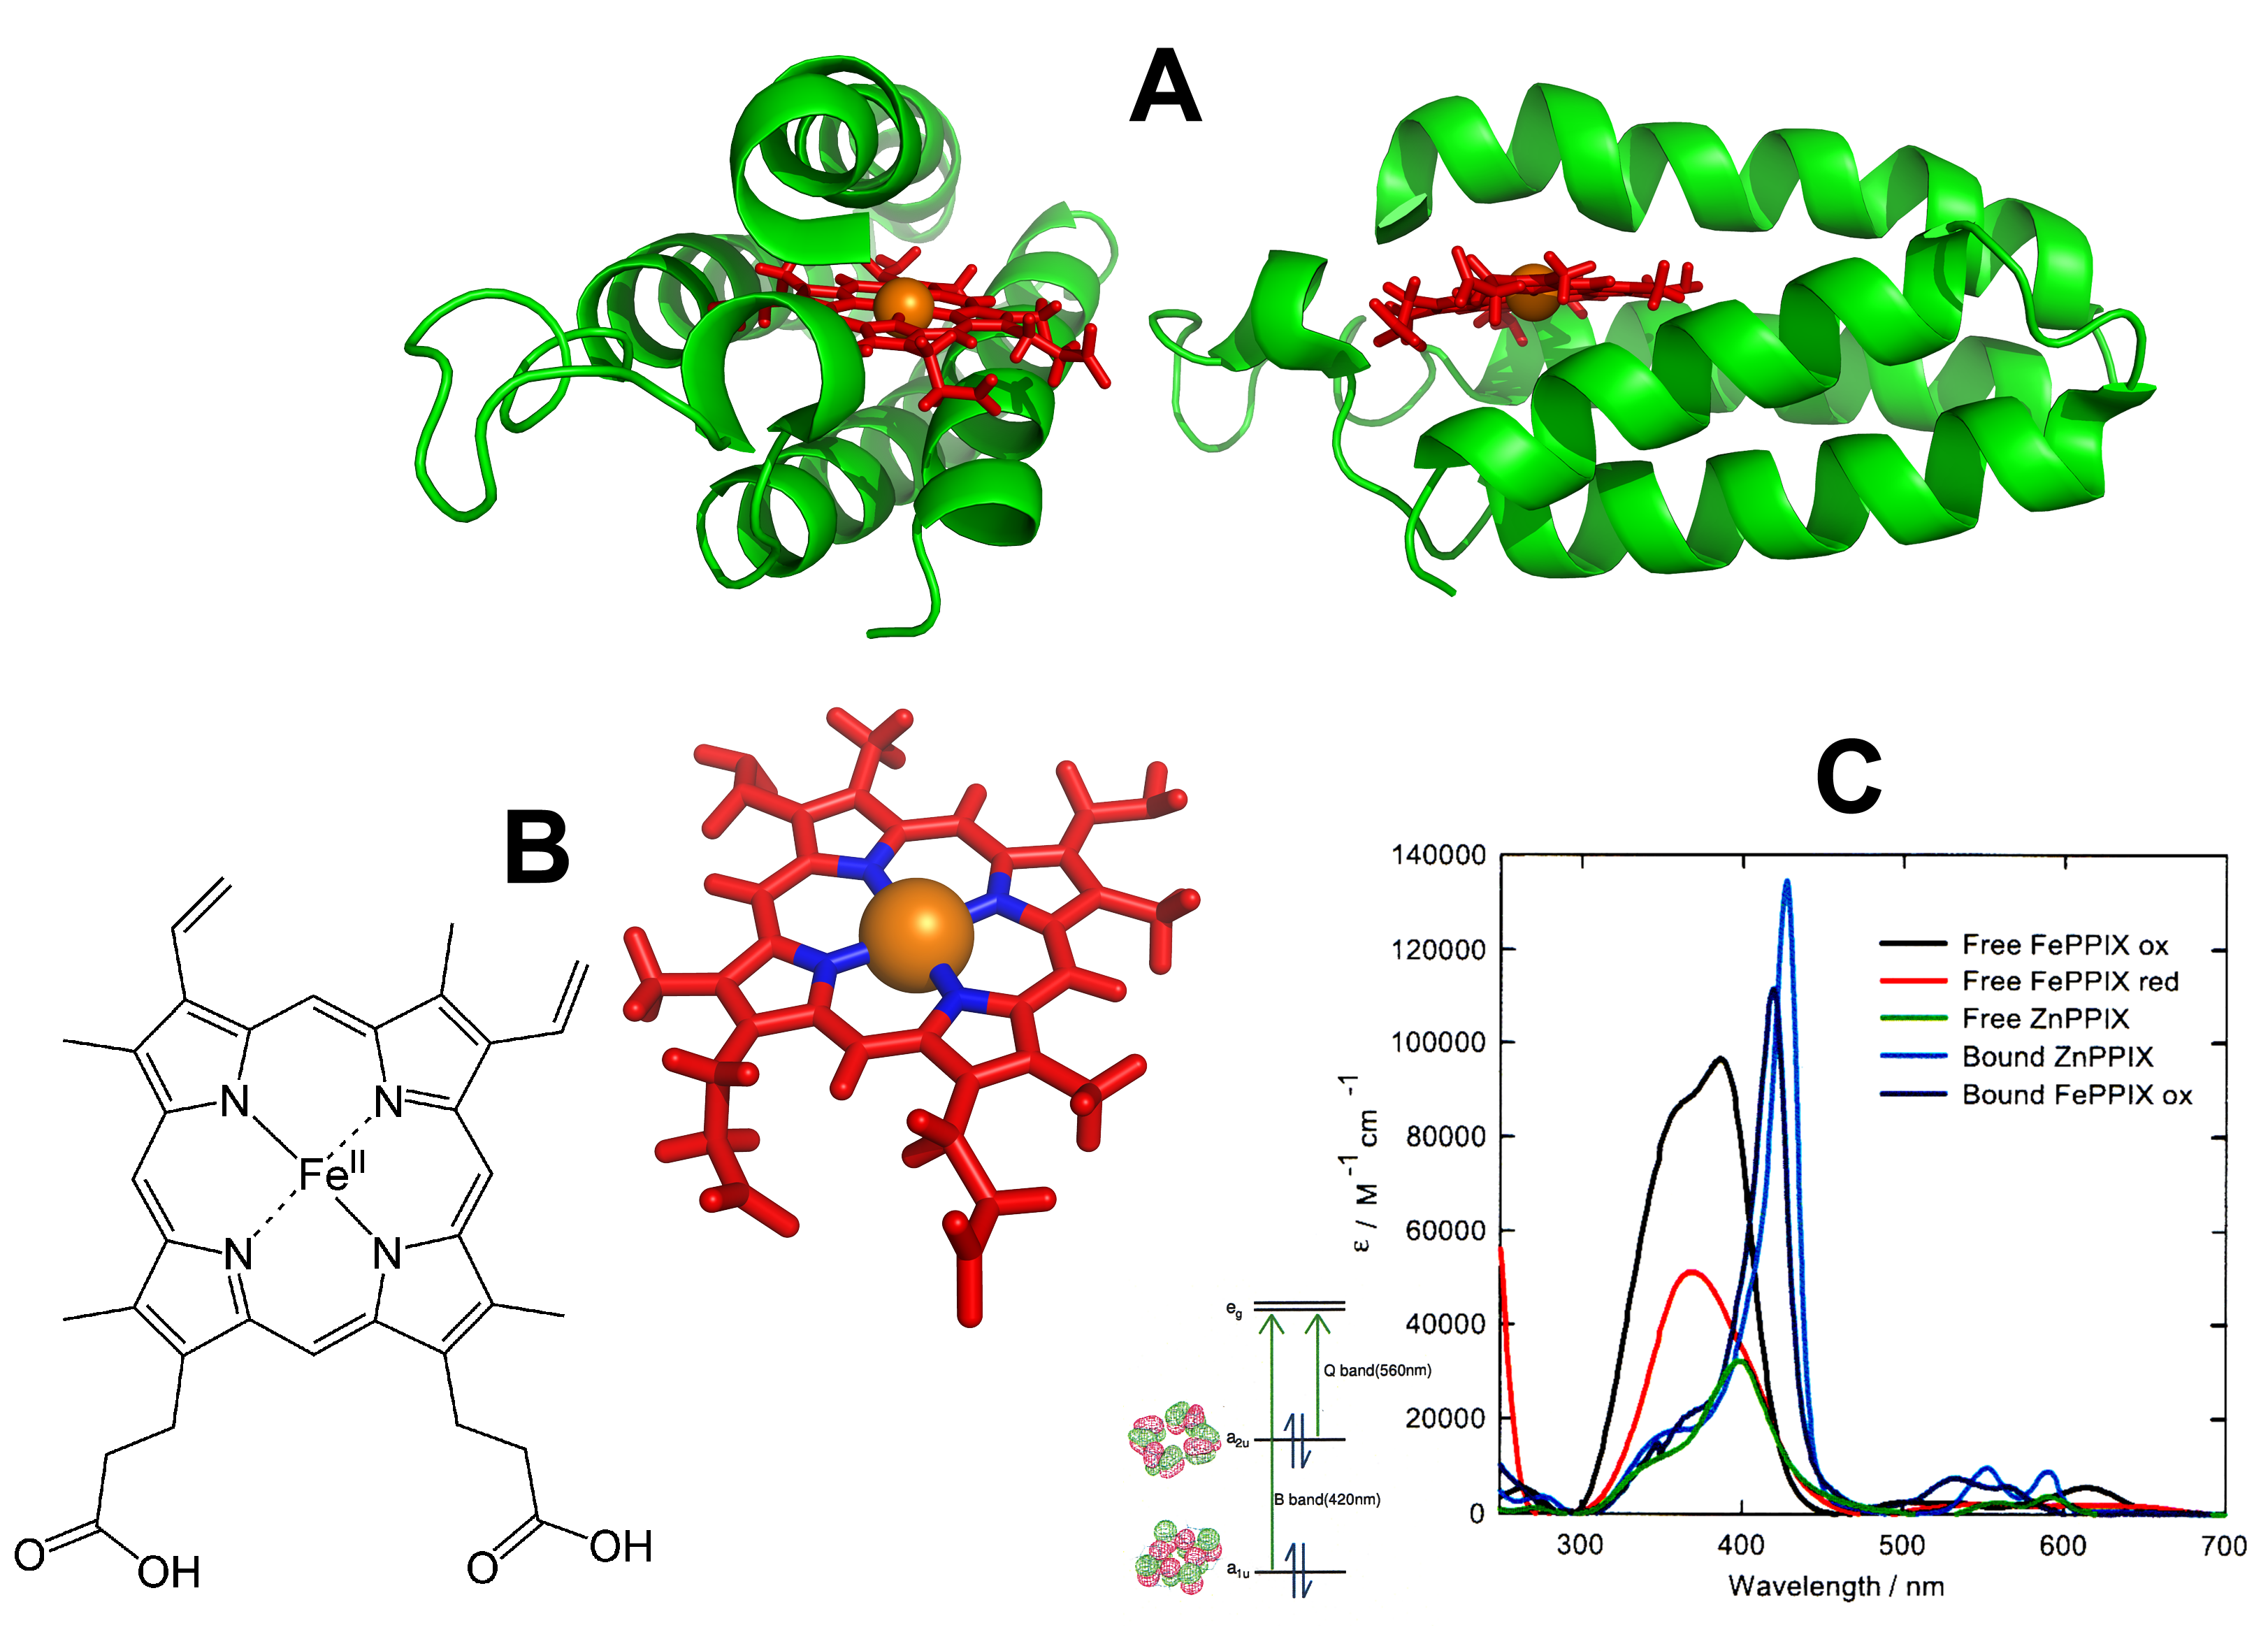
\includegraphics[width=137.4mm]{Images/haemStructure.png}
	\caption[Haem Structure]{A fancy image.}
	\label{fig:haemStructure}
\end{figure}
\end{verbatim}

\vspace{2ex}

\begin{figure}[!th]
	\centering
	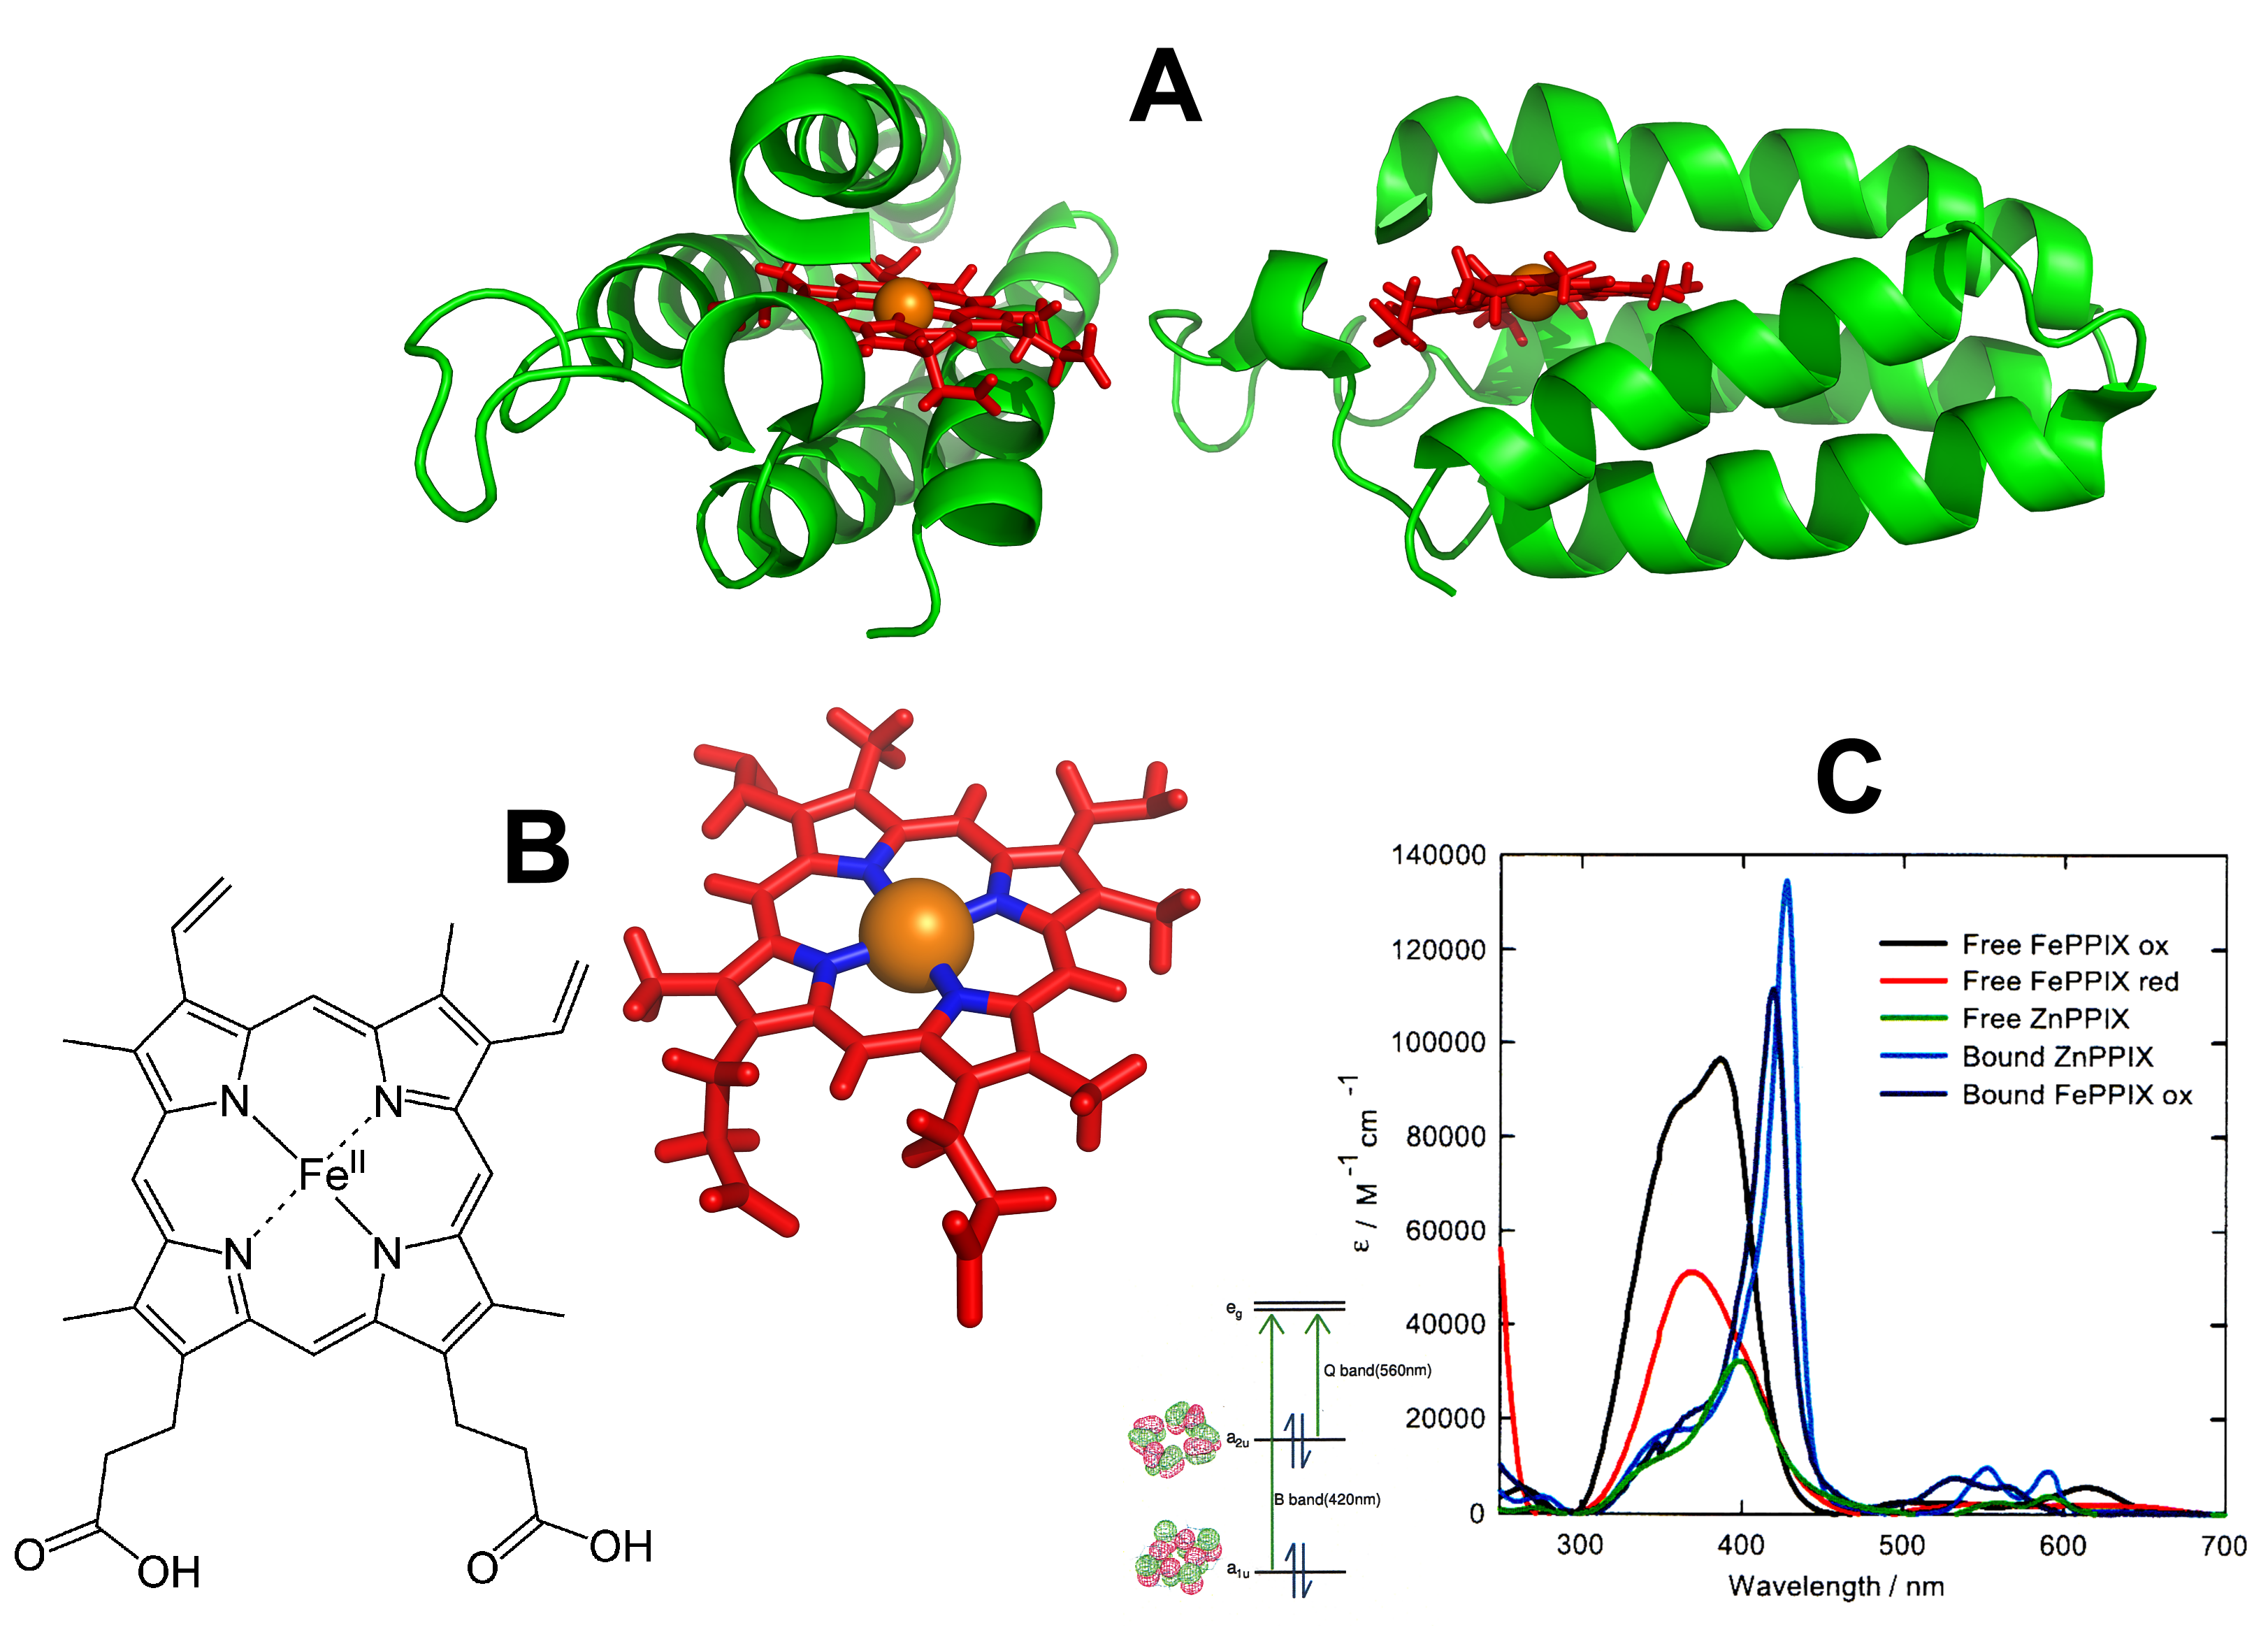
\includegraphics[width=137.4mm]{Images/haemStructure.png}
	\caption[Haem Structure]{A fancy image from Chris' Thesis.}
	\label{fig:haemStructure}
\end{figure}

In this example the command {\textbackslash}includegraphics tells LaTeX to look in the directory `Images' and incorporate the file called `haemStructure.png' into the final document while setting the width to 137.4mm.  This command can be used to resize a graphical file using the height or width parameter as shown. You must specify the units which can be pt, ex, em, mm, cm and so on. LaTeX recognises a very wide variety of standard units and graphics formats. The command is part of the graphicx package and so in the preamble you must include the command {\textbackslash}usepackage\{graphicx\}.

Many packages have been written to provide new commands. For example the `subfigure' package enables you to place separate images or files in the same figure side by side while giving them their own label. However, in this document we only concentrate on the very basics.

\section{Floating Environments}

Both tables and figures are examples of a `floating environments' which means LaTeX decides where to put them. 

The mysterious [!tbh] letters give guidance to LaTeX about roughly where the figure or table is  allowed to be, but in general they can move a long way from where you position them within your text file.  The letters in the square bracket can be t, h or b which stand for top, here or bottom.  If you don't specify any letters LaTeX defaults to [t].

LaTeX will always preserve the order in which figures appear.  If it cannot find a type setting solution, then it may move the float to it's own page, and combine it with other figures. If it still can't fit that in for some reason then it moves the float to the end of the document.  This has the effect of pushing all the remaining floating environments to the end of the document also.

The exclamation mark instructs LaTeX to ``try harder'' at putting the float where you told it to. Often you must play around to ensure the float positioning is acceptable, but usually this can be achieved by stretching or shrinking the image slightly using the size parameter, re-ordering text, judicial applications of the {\textbackslash}pagebreak command or by shouting loudly and slapping the computer monitor about. Note that it is better to resize the image using the original program that was used to create the image. Also using vector graphics can assist be useful (e.g. eps files) because they are designed to scale better.
\chapter{The Chapter on Making Chapters}
\label{sec:Chapters}

Right. LaTeX forces you to structure your document. There a series of simple commands for achieving this:

\vspace*{2ex}

{\textbackslash}chapter\{chapterName\}

{\textbackslash}section\{sectionName\}

{\textbackslash}subsection\{subsectionName\}

{\textbackslash}subsubsection\{subsubsectionName\}

\vspace*{2ex}

Easy enough. At the start of each chapter or section just issue one of these commands to name the section and LaTeX will present the chapter heading in the right style of font, which will be the same style of all the other heading names at that level of hierarchy throughout the document. In addition LaTeX assigns a number to that section. For example, this chapter was created using the command:

\vspace*{2ex}

{\textbackslash}chapter\{The Chapter on Making Chapters\} 

\vspace*{2ex}

LaTeX assigns the correct chapter number to each chapter in turn and then puts it in the table of contents, as you can see by looking at the table of contents! Easy.

\pagebreak
\section{The Section About Sections}
\label{sec:Section}
I think you're getting the hang of this. This section was created using the command {\textbackslash}section\{The Section About Sections\}. It appears in the table of contents as section \ref{sec:Section}.

\subsection{The Sub-Section About Sub-Sections}
\label{sec:SubSection}
Now you're really getting the hang of this. This subsection was created using the command {\textbackslash}subsection\{The Sub-Section About Sub-Sections\}. 

\subsubsection{The Sub-Sub-Section About Sub-Sub-Sections}
\label{sec:SubSubSection}
Now you're really getting the hang of this. but.. caught you out! This subsubsection doesn't have a number!  Ha Ha! It was created using the command {\textbackslash}subsubsection\{The Sub-Sub-Section About Sub-Sub-Sections\} in the same vein as all the other subsections/chapters etc. Here we have stopped the depth of the section numbering at the second level with the command:

\vspace*{2ex}

{\textbackslash}setcounter\{secnumdepth\}\{2\}

\vspace*{2ex}

Easy. WYSIWYM.  LaTeX does what you tell it to do. This is both a blessing and a curse.

\pagebreak
\section*{The Section About Sections That Don't Appear in the Table of Contents}
\label{sec:InvisibleSection}
Ok. Now we're throwing a spanner in the works. This section was created using the command:

\vspace*{2ex}

{\textbackslash}section*\{The Section About Sections That Don't Appear in the Table of Contents\}. 

\vspace*{2ex}

Notice how LaTeX has not assigned a number to the section and it doesn't appear in the table of contents. The effect of the * is to suppress the inclusion of a chapter, section or subsection in the automatic numbering. Easy. You can do this at any level. This is useful for things like prefaces, tables of contents or acknowledgements which you may or may not wish to have an entry in the main contents table. Up to you. It's your thesis. Don't just copy me.

\section{A Small Point About Numbering}

In this section notice how the numbering starts from where it left off before we suppressed the numbering on the previous section. Easy. WYSIWYM.
\pagebreak
\section{The Section About Internal Referencing}
\label{sec:InternalReferencing}

There are two related commands:

\vspace*{2ex}

{\textbackslash}label\{labelName\} 

{\textbackslash}ref\{labelName\}

\vspace*{2ex}


The {\textbackslash}label\{\} command allows you to create a label in a particular environment\footnote{That's right. Chapters, Sections and sub-sections etc are environments!}. The label won't appear in the final document. It's just a label which makes it easy to refer back to any particular environment elsewhere in the document. The {\textbackslash}ref\{\} command enables you to insert a reference anywhere in the document to any label in the document.  For example this is section \ref{sec:InternalReferencing}. The names you use in a label can be anything you like but musn't contain whitespace or special characters. I used the two commands:

\vspace*{2ex}

{\textbackslash}label\{sec:InternalReferencing\}

{\textbackslash}ref\{sec:InternalReferencing\}.

\vspace*{2ex}

The astute among you will realise that LaTeX has to read the document several times. Once to find the labels and then again to populate the references with the correct numbers. So you have to compile a latex document twice to get the referencing right. If there is a missing label or you refer to something that doesn't exist then latex inserts a convenient ? at that point. So hunting for queries is useful way of finding broken references. Latex issues warnings when it finds broken references.

As you create a document you will find yourself putting labels in all over the place so choose a sensible naming convention to help you remember the label names.

Each type of environment (equations, figures, tables, sections etc) has its own independent numbering system.  So when you choose your label name it's a good idea to have an identifier for that type of environment.  I have my own convention for label names which I use to help me remember references. E.g.   sec:SectionAboutCats. Eqn:EquationAboutCats,  Fig:FigureAboutCats and so on. This means you can differentiate between referring to the section or the figure more easily, even though they are about the same thing.

So Internal Referencing is a doddle. Easy!
\chapter{External Referencing}

Referencing is usually performed using a separate program called BibTex.  This program understands the file format .bib.

To create a reference within your document first you must create a .bib file by exporting your list of references from which ever referencing software you used, such as endnote, mendeley or whatever you use.

You can refer to an entry in the .bib file using the {\textbackslash}cite\{ref:Name\} command. the identifier `ref:Name' is the unique identifier which is the first line of each item included in your bibliography file.

For example, open the file LaTexCourseBib.bib in the bibliography directory. The first entry has the identifier `Horcas2007'.  This can be invoked as follows:


\begin{verbatim}
For example, this interesting fact\cite{Horcas2007}, is a cracking example.
\end{verbatim}

For example, this interesting fact\cite{Horcas2007}, is a cracking example.

During compilation latex and bibtex co-operate. During the first compilation latex generates a list of references that it needs.  During the second compilation bibtex populates the details from the .bib file into a shorter, ordered .bib file. The third compilation inserts markers at the right place in the main file and the fourth compilation generates the final list of references. Thus the compilation sequence is latex, bibtex, latex, latex.

The style of the referencing format can be changed using the command {\textbackslash}bibliographyStyle\{\}. e.g. the style used in this document is cjfthesisv1.bst which is invoked by 

\begin{verbatim}
\bibliographystyle{Bibliography/cjfthesisv1}
\end{verbatim}

The location of the list of references in the document is specified by issuing the {\textbackslash}bibliography\{\} command which also specifies the master bibliography file.

\begin{verbatim}
\bibliography{Bibliography/LaTeXCourseBib}
\end{verbatim}




\chapter{Organising Your Files}
One of the drawbacks of word is that the figures and tables are included within the document which becomes very very clunky quite quickly and once it reaches around 100Mb it becomes unwieldy and hard to export. One of that advantages of LaTeX is that the files are all text files and so are very light on resources and are easy to email around the place.

However, sometimes it can be difficult to navigate through a single text file, so if you had a huge document then it becomes difficult to find your way around.  One way of circumnavigating this problem is to break the file up into smaller files. As long as LaTeX knows where to look you can have a file for each logical sub-division of your document.

Therefore it is worth spending a bit of time at the beginning of a large project deciding how you wish to break up your LaTex Files and organise them neatly and tidily.  You can then tell LaTex where to look for the files using the following command:

\vspace*{2ex}
{\textbackslash}include\{fileName\}
\vspace*{2ex}

\pagebreak
\section{Linking a File}
We are now going to copy part of the tutorial file into a separate files and link it the main file.  Because this could go wrong it is sensible to back up tutorial.tex as something else. So save a copy called `tutorialOriginal.tex' for safe keeping. Then follow the following instructions.

\begin{enumerate}
\item Create a new file called MyFirstPage.tex
\item Select and Cut out the first chapter of Tutorial.Tex
\item Paste the first chapter into MyFirstPage.tex
\item Save both tutorial.tex and MyFirstPage.tex
\item Then add {\textbackslash}include\{MyFirstPage\} in tutorial.tex where the text used to be before you cut it out. We don't need to add the `.tex' because LaTeX can only include `.tex' files.
\item compile tutorial.tex and view the PDF
\end{enumerate}

The final PDF should look exactly the same as it was! except we now have a separate file for one of the chapters.

\pagebreak
\section{Creating A Class File}
We can also save our preamble in a separate file called a class file. This makes your main document much easier to understand.  To make it work we need to use the {\textbackslash}LoadClass\{\} command as follows: 

\begin{enumerate}
\item Create another new file and save it as TutorialStyle.cls
\item Copy the preamble of tutorial.tex into the new file. Starting with the {\textbackslash}documentclass{} command and copy right up to, but not including, the {\textbackslash}begin{document} command. Delete the preamble in the original document.
\item Save TutorialStyle.cls and tutorial.tex
\item Modify the first line of TutorialStyle.cls by replacing the word `document' with the word `Load'.
\item Add a new first line of tutorial.tex to use your new style class {\textbackslash}documentclass\{TutorialStyle\}
\item Save both files.
\end{enumerate}

\subsection{Sanity Check}

The first line of TutorialStyle.cls should now be:

\begin{verbatim}
\LoadClass[12pt, oneside, a4paper]{book}
\end{verbatim}
\vspace{2ex}

The first line of tutorial.tex should be:

\begin{verbatim}
\documentClass{TutorialStyle}
\end{verbatim}
\vspace{2ex}

We have just created what is called a style file. You can use this style file as a generic preamble for other documents as well. Compile tutorial.tex.  Nothing should have changed in the final PDF.


\pagebreak
\section{The Structure of this Document}

Lets now look at how I've organised this document. It is identical to my thesis because it started out life as my thesis. I usurped the structure and simply replaced the headings and content to make a kind of reference manual for this introductory course. This document therefore is three things:

\begin{enumerate}
\item An example thesis structure to work from.
\item The LaTeX files which were used to create it can be used as a template for a thesis.
\item It is also a convenient introductory latex manual!
\end{enumerate}

\vspace*{2ex}
Groovy huh?

\section{The Master File}

There is a master file where LaTeX begins the compilation procedure. This contains the {\textbackslash}documentclass command needed to set the ball rolling. Within the file there are a series of {\textbackslash}include\{\} commands, one for each Chapter, which tell LaTeX where to find the files containing each chapter.

The subfiles cannot be compiled on their own because they do not contain the {\textbackslash}documentclass, {\textbackslash}begin\{document\} or {\textbackslash}end\{document\} commands. Lets us look in more detail at the master file and we will learn some new LaTeX commands.

\singlespacing
\pagebreak
\begin{verbatim}
\documentclass{Style/LatexCourseStyle}

\begin{document}
\setcounter{secnumdepth}{2}
\setcounter{tocdepth}{1}

\frontmatter
\onehalfspacing
\include{Frontmatter/Titlepage}
\include{Frontmatter/Declaration}
\include{Frontmatter/Acknowledgements}
\include{Frontmatter/Summary}
\include{Frontmatter/Abbreviations}
\tableofcontents
\listoftables
\listoffigures

\mainmatter
\renewcommand{\sectionmark}[1]{\markright{\thesection \ #1}{}}
\include{Chapters/Overview}
\include{Chapters/MyFirstPage}
\include{Chapters/Lists}
\include{Chapters/mathsEquations}
\include{Chapters/ChemicalEquations}
\include{Chapters/Tables}
\include{Chapters/Figures}
\include{Chapters/Sectioning}
\include{Chapters/externalReferencing}
\include{Chapters/ThesisTemplateMainFile}
%\include{Chapters/ChapterThatIsNotCompiled}

\appendix
%\include{Appendices/UsefulWebsites}

\singlespacing

\backmatter
\addcontentsline{toc}{chapter}{References}
\bibliographystyle{Bibliography/cjfthesisv1}
\renewcommand{\bibname}{References}
\bibliography{Bibliography/LatexCourseBib}

\end{document}
\end{verbatim}
\onehalfspacing
\pagebreak

\section{Analysing the Master File}
Let us go through this file and observe the new commands. Most of it is self-explanatory.

\begin{verbatim}
\documentclass{Style/LaTeXCourseStyle}
\end{verbatim}

This command tells latex that the document class is the one defined in the the style file ''LaTeXCourseStyle'', which is in the sub directory ''style''.  Easy.

\begin{verbatim}
\setcounter{secnumdepth}{2}
\setcounter{tocdepth}{1}
\end{verbatim}

The first of these commands tells latex that the section depth number is 2. I.E. throughout the document only bother numbering sections, subsections and subsubsections down to the second level (such as section 1.2.3). The second command tells latex to only build the table of contents from section numbers down to the first level i.e. 1.1.  Easy enough.

The command {\textbackslash}frontmatter is exclusive to the book class, on which this style is based, and tells latex that within this section to number the pages using roman numerals, and not to include these numbers in the table of contents, just like in a book. The {\textbackslash}mainmatter and {\textbackslash}backmatter commands similarly delineate the other sections of the document.  

Childs play.  How long would it take you to figure out how to do that in word???? No idea. I've never tried.

Note that these rather cool commands are not available in every single class. So for a paper you would use the article class where such compartmentalisation of your document is not appropriate. In fact you can often download latex templates from the journal to wish to submit your paper, which is why I concentrate on the thesis template in this course.

\begin{verbatim}
\onehalfspacing
\end{verbatim}

Is obvious. ''From this point forward use line spacing of one and a half lines please. Thank you.'' How many hours have you spent clicking on paragraph indentations for each separate paragraphs in word? Nightmare. Want to change the standard in the whole document? Not a chance in word. In latex, you can do it with a single word, carefully placed in the master file.

\begin{verbatim}
\include{Frontmatter/Titlepage}
\include{Frontmatter/Declaration}
\include{Frontmatter/Acknowledgements}
\include{Frontmatter/Summary}
\include{Frontmatter/Abbreviations}
\end{verbatim}

The {\textbackslash}include\{\} command tells latex to include the specified .tex file at this point.  Thus it is a simple matter to break up a large document into sub components.  I have written each part of the front matter in a separate file and then grouped all the front matter into one directory called: Frontmatter.

See how the directory structure of my files reflects the structure of my book?

\begin{verbatim}
\tableofcontents
\listoftables
\listoffigures
\end{verbatim}

Again. This is easy. These commands mean: ''Please scan through the whole document and build for me a table of contents, a list of tables, a list of figures and then write down the entries along side their section numbers (as I have them ordered in this version of the document), as well as the page numbers on which they appear and create a nice little summary table and add them to the front matter of my document. Thanks.''.

How does latex do this?  remember the idea of environments?  Well each table, figure, equation etc is a defined environment.  LaTeX just counts them up and assigns numbers starting wherever you want and builds a table.  You can tell latex to ignore individual sections if you want to.

You can also control the look and feel of your table of contents with subtley and grace. Do you want to fill the white space with lines of dots to aid readability, even though the chapter titles are all different lengths? page numbers? How deep should the TOC been?  etc etc etc. How to do this is beyond the scope of this course, but now you know about it, go look it up. easy as $\pi$.

Ok.

Main matter we've done.

\begin{verbatim}
\renewcommand{\sectionmark}[1]{\markright{\thesection \ #1}{}}
\end{verbatim}

This command tells latex to 'renewcommand', i.e. change the meaning of the following command from this point in the document forward, over-riding previous definitions.
\begin{verbatim}
\sectionmark}[1]{\markright{\thesection \ #1}{}
\end{verbatim}

Is latex speak for ``please write the section heading at the top right hand side of each page. thanks''. This works in conjunction with a command in the style file which we'll talk about later. You have to tell latex to switch on headings as well as where to put them.

\begin{verbatim}
\include{Chapters/Overview}
\include{Chapters/MyFirstPage}
\include{Chapters/Lists}
\include{Chapters/mathsEquations}
\include{Chapters/ChemicalEquations}
\include{Chapters/Tables}
\include{Chapters/Figures}
\include{Chapters/Sectioning}
\include{Chapters/externalReferencing}
\include{Chapters/ThesisTemplateMainFile}
%\include{Chapters/ChapterThatIsNotCompiled}
\end{verbatim}

This is the include command again. You will notice that one of the include lines is commented out. This is a handy trick to only build certain parts of my thesis. Which can be useful if individual chapters are being reviewed.

\pagebreak

\begin{verbatim}
\appendix
%\include{Appendices/UsefulWebsites}

\singlespacing

\backmatter
\addcontentsline{toc}{chapter}{References}
\bibliographystyle{Bibliography/cjfthesisv1}
\renewcommand{\bibname}{References}
\bibliography{Bibliography/LatexCourseBib}
\end{verbatim}

The rest is easy. {\textbackslash}Appendix means we are in the appendix now and start labelling sections with A.1.2 instead of 1.2.3.  

{\textbackslash}addcontentsline means forcibly insert a contents line about the references into the contents table. 

{\textbackslash}\{bibliographystyle\{Bibliography/cjfthesisv1\}\} means use the biblography style defined in the file cjfthesisv1. Defining a bibliography style will be covered later if we have time. This is where you specify how the references will appear (names, journals, full stops, commas etc).

{\textbackslash}renewcommand\{{\textbackslash}bibname\}\{References\} means: rename the bibliography chapter as `References'

{\textbackslash}biblography means add the following bibliography.  You can reference entries in this bibliography file very easily.

The astute among you will realise that LaTeX will have to read the document several times before it can be compiled with all the references.  Hey ho. No problem. You can go and have a cuppa while LaTeX does your references for you in the style of your favorite journal... nice.




%\include{Chapters/ChapterThatIsNotCompiled}
\end{verbatim}

This is the include command again. You will notice that one of the include lines is commented out. This is a handy trick to only build certain parts of my thesis. Which can be useful if individual chapters are being reviewed.

\pagebreak

\begin{verbatim}
\appendix
%\include{Appendices/UsefulWebsites}

\singlespacing

\backmatter
\addcontentsline{toc}{chapter}{References}
\bibliographystyle{Bibliography/cjfthesisv1}
\renewcommand{\bibname}{References}
\bibliography{Bibliography/LatexCourseBib}
\end{verbatim}

The rest is easy. {\textbackslash}Appendix means we are in the appendix now and start labelling sections with A.1.2 instead of 1.2.3.  

{\textbackslash}addcontentsline means forcibly insert a contents line about the references into the contents table. 

{\textbackslash}\{bibliographystyle\{Bibliography/cjfthesisv1\}\} means use the biblography style defined in the file cjfthesisv1. Defining a bibliography style will be covered later if we have time. This is where you specify how the references will appear (names, journals, full stops, commas etc).

{\textbackslash}renewcommand\{{\textbackslash}bibname\}\{References\} means: rename the bibliography chapter as `References'

{\textbackslash}biblography means add the following bibliography.  You can reference entries in this bibliography file very easily.

The astute among you will realise that LaTeX will have to read the document several times before it can be compiled with all the references.  Hey ho. No problem. You can go and have a cuppa while LaTeX does your references for you in the style of your favorite journal... nice.




%\include{Chapters/ChapterThatIsNotCompiled}
\end{verbatim}

This is the include command again. You will notice that one of the include lines is commented out. This is a handy trick to only build certain parts of my thesis. Which can be useful if individual chapters are being reviewed.

\pagebreak

\begin{verbatim}
\appendix
%\include{Appendices/UsefulWebsites}

\singlespacing

\backmatter
\addcontentsline{toc}{chapter}{References}
\bibliographystyle{Bibliography/cjfthesisv1}
\renewcommand{\bibname}{References}
\bibliography{Bibliography/LatexCourseBib}
\end{verbatim}

The rest is easy. {\textbackslash}Appendix means we are in the appendix now and start labelling sections with A.1.2 instead of 1.2.3.  

{\textbackslash}addcontentsline means forcibly insert a contents line about the references into the contents table. 

{\textbackslash}\{bibliographystyle\{Bibliography/cjfthesisv1\}\} means use the biblography style defined in the file cjfthesisv1. Defining a bibliography style will be covered later if we have time. This is where you specify how the references will appear (names, journals, full stops, commas etc).

{\textbackslash}renewcommand\{{\textbackslash}bibname\}\{References\} means: rename the bibliography chapter as `References'

{\textbackslash}biblography means add the following bibliography.  You can reference entries in this bibliography file very easily.

The astute among you will realise that LaTeX will have to read the document several times before it can be compiled with all the references.  Hey ho. No problem. You can go and have a cuppa while LaTeX does your references for you in the style of your favorite journal... nice.




%\include{Chapters/External Referencing}

\appendix
%\include{Appendices/UsefulWebsites}

\singlespacing

\backmatter
%\addcontentsline{toc}{chapter}{References}
%\bibliographystyle{Bibliography/cjfthesisv1}
%\renewcommand{\bibname}{References}
%\bibliography{Bibliography/LatexCourseBib}

\end{document}  
\end{verbatim}
\onehalfspacing
\pagebreak

\section{Analysing the Master File}
Let us go through this file and observe the new commands. Most of it is self-explanatory.

\begin{verbatim}
\documentclass{Style/LaTeXCourseStyle}
\end{verbatim}

This command tells latex that the document class is the one defined in the the style file ''LaTeXCourseStyle'', which is in the sub directory ''style''.  Easy.

\begin{verbatim}
\setcounter{secnumdepth}{2}
\setcounter{tocdepth}{1}
\end{verbatim}

The first of these commands tells latex that the section depth number is 2. I.E. throughout the document only bother numbering sections, subsections and subsubsections down to the second level (such as section 1.2.3). The second command tells latex to only build the table of contents from section numbers down to the first level i.e. 1.1.  Easy enough.

The command {\textbackslash}frontmatter is exclusive to the book class, on which this style is based, and tells latex that within this section to number the pages using roman numerals, and not to include these numbers in the table of contents, just like in a book. The {\textbackslash}mainmatter and {\textbackslash}backmatter commands similarly delineate the other sections of the document.  

Childs play.  How long would it take you to figure out how to do that in word???? No idea. I've never tried.

Note that these rather cool commands are not available in every single class. So for a paper you would use the article class where such compartmentalisation of your document is not appropriate. In fact you can often download latex templates from the journal to wish to submit your paper, which is why I concentrate on the thesis template in this course.

\begin{verbatim}
\onehalfspacing
\end{verbatim}

Is obvious. ''From this point forward use line spacing of one and a half lines please. Thank you.'' How many hours have you spent clicking on paragraph indentations for each separate paragraphs in word? Nightmare. Want to change the standard in the whole document? Not a chance in word. In latex, you can do it with a single word, carefully placed in the master file. Grace personified. 

In fact in general in latex you can override global settings locally.  This is v. useful. Just switch it on and off at will as required.

\begin{verbatim}
\thispagestyle{empty}

\begin{center}
\vspace*{\stretch{1}}

\hrule height 2pt
\vspace*{2ex}
{\Huge\textbf{Towards the Ability to Make Super Duper LaTeX Documents}\par}
\vspace*{2ex}
\hrule height 2pt
\vspace*{10ex}
{
\includegraphics[height=40mm]{Images/UnivShield}\par}
\vspace*{10ex}
{\large\textbf{Christopher~James~Forman}\par}
\vspace*{2ex}
{\large{Department Of Chemistry}\par}
\vspace*{2ex}
{\large{University of Cambridge}\par}
\vspace*{5ex}
{\large{This dissertation is submitted for the degree of \textit{Doctor of Philosophy}}\par}
\vspace*{5ex}
{\large{\today}\par}

\vspace*{\stretch{2}}
\end{center}
\chapter*{Declaration}

\vfill

This dissertation is the result of my own work and includes nothing which is the outcome of work done in collaboration except where specifically indicated in the text. It is not substantially the same as any that I have submitted for a degree or diploma or other qualification at any other University and no part has already been, or is concurrently being, submitted for any degree, diploma, or other qualification. It does not exceed 60,000 words, including tables, footnotes, bibliography and appendices.\par

\vspace{10ex}

\begin{flushright}
Signature: \rule[0pt]{60mm}{0.5pt}

\vspace{5ex}

Date: \rule[0pt]{60mm}{0.5pt}
\end{flushright}

\vfill
\chapter*{Acknowledgments}
\subsection*{Family}
Mum. Dad. Pet Dog.

\subsection*{Scientific Collaborations}
Dr A.N.Other at uni of blah for samples and instrument time etc. My Amazing Lab Chums.

\subsection*{Scientific Support}
My amazing lab chums.

\subsection*{General Assistance}
Cleaner, My amazing lab chums.

\subsection*{Financial Support}
Bank, Tax payer. My amazing lab chums.

\subsection*{Moral Support}
My Amazing Lab chums.

\subsection*{Academic Inspiration}
Netwon, My super. My Amazing Lab Chums.

\subsection*{Everyone else}
My Amazing Lab Chums.

\chapter*{Summary}
This document is a handbook for introducing you to LaTeX. It contains a bit of background about the history and philosophy of LaTeX.  However, it concentrates on providing a guided practical introduction to the basic techniques such as 
\begin{itemize}
\item Lists
\item Mathematical and chemical equations
\item Tables
\item Figures
\item Chapters and Sections
\item Linking to other files in large documents
\item Referencing
\end{itemize}

The handbook is also presented in the style of a thesis. This means that source files provided on the introductory course and available from the department web page are a convenient template for a thesis.

More details on specific aspects of LaTeX can be found at the departmental LaTeX page which can be found here:

 http://www-ch-int.ch.private.cam.ac.uk/latex/about

\chapter*{Abbreviations}

\begin{longtable}{r >{\rule{0pt}{3ex}}l<{\rule[-1.5ex]{0pt}{0pt}}}
ADP & Adenosine Diphosphate\\
(nc/c)AFM & (non-contact/conducting) Atomic Force Microscopy\\
ATP & Adenosine Triphosphate \\
\end{longtable}
\end{verbatim}

The {\textbackslash}include\{\} command tells latex to include the specified .tex file at this point.  Thus it is a simple matter to break up a large document into sub components.  I have written each part of the front matter in a separate file and then grouped all the front matter into one directory called: Frontmatter.

See how the directory structure of my files reflects the structure of my book?

This is so easy and flexible it's unbelievable that humans are smart enough to come up with this stuff...

\begin{verbatim}
\tableofcontents
\listoftables
\listoffigures
\end{verbatim}

Again. This is easy. These commands mean: ''Please LaTeX, at this point in the creation of my document could you scan through the whole document and build for me a table of contents, a list of tables, a list of figures and then write down the entries along side their section numbers (as I have them ordered in this version of the document), as well as the page numbers on which they appear and create a nice little summary table and add them to the front matter of my document. Thanks.''.

How does latex do this?  remember the idea of environments?  Well each table, figure, equation etc is a defined environment.  LaTeX just counts them up and assigns numbers starting wherever you want and builds a table.  You can tell latex to ignore individual sections if you want to.

You can also control the look and feel of your table of contents with subtley and grace. Do you want to fill the white space with lines of dots to aid readability, even though the chapter titles are all different lengths? page numbers? How deep should the TOC been?  etc etc etc. How to do this is beyond the scope of this course, but now you know about it, go look it up. easy as pie.

Ok.

Main matter we've done.

\begin{verbatim}
\renewcommand{\sectionmark}[1]{\markright{\thesection \ #1}{}}
\end{verbatim}

This command tells latex to 'renewcommand', i.e. change the meaning of the following command from this point in the document forward, over-riding previous definitions.
\begin{verbatim}
\sectionmark}[1]{\markright{\thesection \ #1}{}
\end{verbatim}

Is latex speak for ``please write the section heading at the top right hand side of each page. thanks''. This works in conjunction with a command in the style file which we'll talk about later. You have to tell latex to switch on headings as well as where to put them.

\begin{verbatim}
\chapter{Overview}
\label{chap:overview}
\section{LaTeX: The answer to everything.}
LaTeX is typsetting program that takes an input file of marked up text and then, with a user defined set of rules, typesets a beautifully crafted output file that can be easily printed (e.g. a pdf). 

\subsection{Advantages}

The advantages of this method are manifold:

\begin{itemize}

\item Use any text editor to view the source document.
\item More time can be spent working on the content and not worrying about how text or figures interact in the layout until later on.
\item LaTeX uses consistent rules throughout a document
\item LaTeX sorts out basic typesetting automatically
\item Changes can be introduced globally with very little effort
\item Document structure is explicit
\item Documents can be professionally typeset and look great
\item You are forced to structure your documents correctly.
\item Mathematical equations, like $E=mc^2$ or $\imath\hbar\frac{\partial}{\partial t}\Phi (x, t) = \hat{H}\Phi (x, t)$ can be produced almost as fast as typing (if you know the commands!).
\end{itemize}

\subsection{Disadvantages}
The disadvanatges of this method are also manifold:
\begin{itemize}
\item You don't see the output as you go.
\item Steep learning curve.
\item Documents are harder to edit by a second author (unless they are adept at LaTeX too). This can be mitigated using version control, which makes group authoring processes superior to word.
\item The program never works quite the way you want it to and learning how to influence it can be problematic and subtle.
\item Although intended to save work the principle of 'conservation of work' means that you simply transform problems associated with WYSISYG approaches to problems associated with WYSIWYM approaches!
\item You can go blind trying to determine the difference between wiggly and smooth brackets if your editors font isn't large enough.
\end{itemize}

\subsection{On balance?}
If it's so rubbish, why use LaTeX?

\begin{itemize}
\item Large documents are much more easily handled. 
\item In general it is quicker to debug a LaTeX document than typeset an entire thesis manually. 
\item Technical information such as tables, equations and figures are integrated much more smoothly than with word.
\end{itemize}

\section{How does it work?}

The raw text is interspersed with commands, preceded by a \textbackslash, which tell LaTeX what to do with the text. For example you can \textbf{make it bold}, \emph{italic}, or \underline{underlined} with the commands {\textbackslash}textbf\{\}, {\textbackslash}emph\{\} or {\textbackslash}underlined\{\}. More on commands in a moment...



\chapter{My First Page}

\section{The Very Beginning}
The very simplest LaTeX document might look like this:

\begin{verbatim}
\documentclass[a4paper,12pt]{article}
\begin{document}
Hello World.
\end{document}
\end{verbatim}

\pagebreak
\thispagestyle{empty}
Hello World.
\pagebreak
\subsection{Break Down}
What's all the gobbledegook around my simple message???

In LaTeX we intersperse text and commands.  Commands are preceded by a \textbackslash. For example the first line in a LaTeX document \underline{\textbf{\emph{must}}} be:

\begin{verbatim}
\documentclass[options]{class}
\end{verbatim}

Where the word ''class'' may be substituted for one of many things such as: article, proc, minimal, report, book, letter, memoir, slides, beamer.

Similarly, and completely generally in LaTeX speak, the square brackets denote the existence of optional parameters. Each individual command can take its own parameters and for the ''{\textbackslash}documentclass'' command there are options for controlling font size, font family, landscape, oneside, twosided, page size and so on. These options will persist throughout the entire document. For example the document class command for this document, (which is likely to be like the one you would use for a thesis), would be:

\begin{verbatim}
\documentclass[12pt, oneside, a4paper]{book}
\end{verbatim}

Other options include:

\begin{itemize}
\item {10pt, 11pt, 12pt (default is 10pt).}
\item {letterpaper, legalpaper, a4paper, executivepaper, a5paper, b5paper}
\end{itemize}
and so on.

\pagebreak
\section{Can I start typing please?}

After we have set up the document we can start actual work on our document. So we must tell LaTeX that what follows is to be interpreted as a document.  The command {\textbackslash}begin can take many different parameters and is a command to enter what is known, in LaTeX speak, as 'an environment'. Thus the commands:
\begin{verbatim}
\begin{document}

\end{document}
\end{verbatim}

tells LaTeX to enter and leave the document environment, and thus constitute the outer limits of our document file. Other environments include the equation environment, the itemize environment, the figure environment and so on. These will be encountered in due course.

Every part of the LaTeX file is therefore within an environment of specific type and the content within each environment consists of commands or text.

That's basically it.

So let's get on with it shall we...

\pagebreak
\section{The ground rules}
\begin{quote}
Hold on, hold on, hold on my son.

First the lessons.

Then the fun!
\end{quote}
Dr Seuss.

\subsection{Spaces}
Whitespace characters, such as blank or tab, are treated uniformly as space by LaTeX. Several consecutive whitespace characters are treated as one single space. Whitespace at the start of a line is generally ignored, and a single line break is treated as whitespace. An empty line between two lines of text defines the end of a paragraph. Several empty lines are treated the same as one empty line. The text below is an example.

\begin{verbatim}
It does not matter whether you
enter one or several             spaces
after a word. The final result will be typeset beautifully
according    to     precise rules.




An empty line starts a new
paragraph. Note the indentation on the first line of the paragraph, 
except at the beginning of the section. 
\end{verbatim}

\vspace*{2ex}
\vspace*{2ex}

It does not matter whether you
enter one or several             spaces
after a word. The final result will be typeset beautifully
according    to     specific rules.




An empty line starts a new
paragraph. Note the indentation on the first line of the paragraph, except at the beginning of the section. 

\pagebreak
\subsection{Special Characters}
The symbols 

\# \$ \% \textasciicircum{} \& \_ \{ \} \~{} \textbackslash

are reserved characters that either have a special meaning under LaTeX or are unavailable in all the fonts. If you enter them directly in your text, they will normally not print, but rather make LaTeX do strange things.

To overide the special meanings of these symbols and allow them to produced within your text you may use the following sequences:
\begin{verbatim}
\# \$ \% \textasciicircum{} \& \_ \{ \} \~{} \textbackslash
\end{verbatim}

Other symbols and many more can be printed with special commands in mathematical formulae or as accents.

The backslash character '\textbackslash' cannot be entered by adding another backslash in front of it ( \textbackslash\textbackslash); because this sequence means ''linebreak''.

The command \textbackslash\~{}\{\} produces a tilde which is placed over the next letter. For example \textbackslash\~{}\{n\} gives \~{n}. To produce just the character \~{}, use \textbackslash\~{}\{\} which places a \~{} over an empty box.

Similarly, the command \textbackslash\textasciicircum{} produces a hat over the next character, for example \textbackslash\textasciicircum\{o\} produces \^{o}.

\pagebreak
\section{Preamble}
After the {\textbackslash}documentclass command we add ''preamble''. Here we load special features that we will use throughout our document to expand on the basic capabilities of LaTex. These are contained in units called ''packages'' which we can tell our LaTeX compiler to download by using the command ''{\textbackslash}include\{packageName\}''. 

There are many repositories of such packages on the web. Your compiler generally knows where to look and most standard packages are included with any install. For example, to include a special set of typesetting instructions to handle chemical equations we can grow our simple document with a single command like this:

\begin{verbatim}
\documentclass[a4paper,12pt]{article}
\usepackage[version=3]{mhchem}
\begin{document}
Hello World!

We all need \ce{H2O}.

I'm less fussed about \ce{^{235}_{92}U+}.

\end{document}
\end{verbatim}

\vspace{2ex}

\pagebreak
\thispagestyle{empty}
Hello World!

We all need \ce{H2O}.

I'm less fussed about \ce{^{235}_{92}U+}.
\pagebreak

Here we have loaded a package called: "`mhchem"' which took the option ''[version=3]''. This is a package for drawing chemical equations easily and it has it's own instruction manual which you can follow easily. It is included in the bundle of files for this course.

Other things we can do in the premable within LaTeX are to redefine existing commands or create our own personal commands. These can be stored in a file called the 'style file' which we can load at the beginning of our document, in place of our documentclass. More about this later on...


\subsection{Comments}
It is often useful to comment your LaTeX documents. You can leave yourself amusing, sarcastic messages that won't get printed out in the final document. Use this to make your own notes as the course progresses.

To get a comment use the \% command, which tells LaTeX to ignore the rest of the line, the line break and all the white space at the beginning of the next line, for example, we may add to our continually evolving document...

\begin{verbatim}
\documentclass[a4paper,12pt]{article}
\usepackage[version=3]{mhchem}
\begin{document}
Hello World!

%All humans need water and I would like 
%to include this concept in my arguments.
We all need \ce{H2O}.

%Uranium 235 is toxic, which is why I don't want to consume it... 
I'm less fussed about \ce{^{235}_{92}U+}.

\end{document}
\end{verbatim}

\vspace{4ex}
Hello World!

%All humans need water and I would like to include this concept in my arguments.
We all need \ce{H2O}.

%Uranium 235 is toxic, which is why I don't want to consume it... 
I'm less fussed about \ce{^{235}_{92}U+}.

\pagebreak
\section{Compiling}
Once the document is finished you can compile it. Your compiler will depend on the platform that you use. In the PWF we are using winEDT to edit the documents (a LaTeX front end) and texlive2008 which is the compiler itself. I use MiKTex and the front end texCenter.  There is no need to use a front end. If you prefer you can use a simple text editor and a command line.

the recommended distributions are:
\begin{itemize}
\item MiKTeX or TeX Live for Windows
\item TeX Live for Unix/Linux
\item MacTeX or TeX Live for Mac OS.
\end{itemize}

Once you have installed your software and got it working, written your source code and tried to compile it, there will nearly always be something wrong with your file. 

Any errors will be highlighted in the console window or error output box of your front end.  Some front ends dump the running commentary which LaTeX produces into a text file for easy reading afterwards.

In a compile attempt (successful or otherwise) LaTeX may produce the following files:

projectname.aux

projectname.bbl

projectname.lof

projectname.lot

projectname.txt

projectname.toc

projectname.dvi

These are interim files (toc= table of contents, bbl = bibliography etc). To be honest I have no idea what half of these things contain.  You only need the .tex file and a compiler with the right packages installed to produce them again.

Some versions of LaTeX only produce DVI files and you then need to convert the dvi file to a PDF or download a dvi viewer. You can also convert DVI files to PS files and then view them.  The good thing about front ends is that you can set them up to produce PDFs directly.

OK. So we have now produced a silly document but we understand it.  Now lets get on with learning how to make our own documents.



\chapter{Lists}
Lists are great.  The command {\textbackslash}begin\{\} can be used to enter a list environment.  For example:

\begin{verbatim}
\begin{itemize}
\item cat
\item dog
\item horse
\end{itemize}
\end{verbatim}

Produces:

\begin{itemize}
\item cat
\item dog
\item horse
\end{itemize}

\pagebreak
We can also replace the bullet points with numbers using the enumerate keyword.

\begin{verbatim}
\begin{enumerate}
\item cat
\item dog
\item horse
\end{enumerate}
\end{verbatim}

\begin{enumerate}
\item cat
\item dog
\item horse
\end{enumerate}

\pagebreak
and we can use the description keyword which does this:
\begin{verbatim}
\begin{description}
\item[Cat] a lovely furry creature with a cute nose and whiskers.
\item[Dog] Another furry creature that smells rather well; 
           its olfactory power stems from its nasal dampness.
\item [Horse] A large stinky creature with sideways facing eyes.
\end{description}
\end{verbatim}

\begin{description}
\item[Cat] a lovely furry creature with a cute nose and whiskers.
\item[Dog] Another furry creature that smells rather well; its olfactory power stems from its nasal dampness.
\item [Horse] A large stinky creature with sideways facing eyes.
\end{description}
\chapter{Tables}
Tables are big business in Latex.  I use these packages to help me.

\begin{verbatim}
\usepackage{multirow}
\usepackage{booktabs}
\usepackage{dcolumn}
\end{verbatim}

Here's an example table

\begin{table}[!hb]
 \centering
	\begin{tabular}{@{}rccc@{~}r@{.}l*3{r@{.}l@{~}r@{.}l}D{.}{\cdot}{2,1}}
	\toprule
	\multicolumn{1}{c}{Fibre Type}
	& N 
	& M 
	&\multicolumn{3}{c}{$L_t$ (nm)}
	&\multicolumn{4}{c}{$R_t$ (nm)}
	&\multicolumn{4}{c}{$d_t$ (nm)}
	&\multicolumn{4}{c}{${\Delta}Z_t$ (nm)}
	&\multicolumn{1}{c}{~}\\
\cmidrule(lr){1-1}
\cmidrule(lr){2-2}
\cmidrule(lr){3-3}
\cmidrule(lr){4-6}
\cmidrule(lr){7-10}
\cmidrule(lr){11-14}
\cmidrule(lr){15-18}
  SS Twisted & 5 & 4 & 313 &\multicolumn{2}{c}{(122)} & 5&7 &(1&6)  & 5&4 &(1&0)  &  150&5 &(63&1) &\multicolumn{1}{c}{~} \\
  \multicolumn{19}{c}{~}\\
  %\cmidrule(lr){3-18}
  &
  &
 	&\multicolumn{3}{c}{$L_s$ (nm)} 
 	&\multicolumn{4}{c}{$R_s$ (nm)}
 	&\multicolumn{4}{c}{$W_s$ (nm)}
 	&\multicolumn{4}{c}{${\Delta}Z_s$ (nm)}
 	&\multicolumn{1}{c}{${\Delta}Z_{e}$ (nm)}\\
\cmidrule(lr){4-6}
\cmidrule(lr){7-10}
\cmidrule(lr){11-14}
\cmidrule(lr){15-18}
\cmidrule(lr){19-19}
  SS Spiral& 32 & 7 &123&(31&6)&11&4&(3&3)&11&1&(2&6)&32&9&(22&2)&26.9\\
  SSB Spiral& 64&18 &106&(22&9)&10&8&(2&7)&9&8&(1&8)&28&2&(8&1)&22.7\\
	%\midrule
  BSS Spiral&37 &19 &110&(44&9)&13&4&(3&0)&12&9&(1&8)&27&1&(9&1)&21.5\\
	%\midrule
  SSSB Spiral&26& 6 &104&(23&9)&13&3&(2&6)&16&4&(3&4)&29&9&(11&1)&22.5\\
	\bottomrule
	\end{tabular}	
	\caption[Basic Fibre Dimensions by TEM]{A funky table from my thesis.}
	\label{tab:BasicXSBFibreDimensionsTEM}
\end{table}

\pagebreak
Here's what the code looks like:
\begin{verbatim}
\begin{table}[!hb]
 \centering
	\begin{tabular}{@{}rccc@{~}r@{.}l*3{r@{.}l@{~}r@{.}l}D{.}{\cdot}{2,1}}
	\toprule
	\multicolumn{1}{c}{Fibre Type}
	& N 
	& M 
	&\multicolumn{3}{c}{$L_t$ (nm)}
	&\multicolumn{4}{c}{$R_t$ (nm)}
	&\multicolumn{4}{c}{$d_t$ (nm)}
	&\multicolumn{4}{c}{${\Delta}Z_t$ (nm)}
	&\multicolumn{1}{c}{~}\\
\cmidrule(lr){1-1}
\cmidrule(lr){2-2}
\cmidrule(lr){3-3}
\cmidrule(lr){4-6}
\cmidrule(lr){7-10}
\cmidrule(lr){11-14}
\cmidrule(lr){15-18}
  SS Twisted & 5 & 4 & 313 &\multicolumn{2}{c}{(122)} & 5&7 &(1&6)  & 5&4 &(1&0)  &  150&5 &(63&1) &\multicolumn{1}{c}{~} \\
  \multicolumn{19}{c}{~}\\
  %\cmidrule(lr){3-18}
  &
  &
 	&\multicolumn{3}{c}{$L_s$ (nm)} 
 	&\multicolumn{4}{c}{$R_s$ (nm)}
 	&\multicolumn{4}{c}{$W_s$ (nm)}
 	&\multicolumn{4}{c}{${\Delta}Z_s$ (nm)}
 	&\multicolumn{1}{c}{${\Delta}Z_{e}$ (nm)}\\
\cmidrule(lr){4-6}
\cmidrule(lr){7-10}
\cmidrule(lr){11-14}
\cmidrule(lr){15-18}
\cmidrule(lr){19-19}
  SS Spiral& 32 & 7 &123&(31&6)&11&4&(3&3)&11&1&(2&6)&32&9&(22&2)&26.9\\
  SSB Spiral& 64&18 &106&(22&9)&10&8&(2&7)&9&8&(1&8)&28&2&(8&1)&22.7\\
	%\midrule
  BSS Spiral&37 &19 &110&(44&9)&13&4&(3&0)&12&9&(1&8)&27&1&(9&1)&21.5\\
	%\midrule
  SSSB Spiral&26& 6 &104&(23&9)&13&3&(2&6)&16&4&(3&4)&29&9&(11&1)&22.5\\
	\bottomrule
	\end{tabular}	
	\caption[Basic Fibre Dimensions by TEM]{A funky table from my thesis.}
	\label{tab:BasicXSBFibreDimensionsTEM}
\end{table}
\end{verbatim}

\pagebreak

\section{Tables Made Easy}
Here is a simple table followed by the code that produced it.

\begin{center}
\begin{tabular}{lcr}
anchovy & banana & carrot \\
dog & apple & fennel \\
goat & strawberry & potato
\end{tabular}

\vspace*{2ex}

\begin{verbatim}
\begin{tabular}{lcr}
anchovy & banana & carrot \\
dog & apple & fennel \\
goat & strawberry & potato
\end{tabular}
\end{verbatim}
\end{center}

\vspace*{2ex}

The tabular environment is a special case of the ''array'' environment for distributing content uniformly across a region of the page.  This ability has already been exploited to align mathematical equations. For now though look at the first line.

\vspace*{2ex}

\begin{verbatim}
\begin{tabular}{lcr}
\end{verbatim}

\vspace*{2ex}

This command tells LaTeX to enter the tabular environment. The letters l, c and r in the curly braces tell LaTeX to create a table with three columns in which the first column is left justified, the second column is centered and the third column is right justified. Lets add a fourth column and this time center justify all the columns.

\begin{center}
\begin{tabular}{cccc}
anchovy & banana & carrot & Johnny\\
dog & apple & fennel & Pete\\
goat & strawberry & potato &
\end{tabular}

\vspace*{2ex}

\begin{verbatim}
\begin{tabular}{cccc}
anchovy & banana & carrot & Johnny\\
dog & apple & fennel & Pete\\
goat & strawberry & potato &
\end{tabular}
\end{verbatim}
\end{center}

\vspace*{2ex}

Each row in the table is a list of items separated by the {\&} symbol. The end of each row is denoted by \textbackslash\textbackslash.  The last row in the table doesn't have a \textbackslash\textbackslash. You do not have to have data between the ampersands but you must have the right number of ampersands to match the number of columns that LaTeX is expecting.

\subsection{Adding Borders To Tables}
\label{sec:vertLines}
Tables should never have vertical lines. No professionally typeset table contains vertical lines. Do not put vertical lines in your tables. That said it is easy to do.

\begin{center}
\begin{tabular}{|c|c|c|c|}
anchovy & banana & carrot & Johnny\\
dog & apple & fennel & Pete\\
goat & strawberry & potato &
\end{tabular}

\vspace*{2ex}

\begin{verbatim}
\begin{tabular}{|c|c|c|c|}
anchovy & banana & carrot & Johnny\\
dog & apple & fennel & Pete\\
goat & strawberry & potato &
\end{tabular}
\end{verbatim}
\end{center}

\vspace*{2ex}

Tables should have neatly headed columns with the heading for each field separated from the data by horizontal lines. The {\textbackslash}toprule, {\textbackslash}cmidrule{} and {\textbackslash}bottomrule commands from the booktabs package are useful for controlling horizontal lines.

\begin{center}
\begin{tabular}{cccc}
\toprule
Ingredient 1 & Ingredient 2 & Ingredient 3 & Source \\
\cmidrule(){1-4}
anchovy & banana & carrot & Johnny\\
dog & apple & fennel & Pete\\
goat & strawberry & potato & \\
\bottomrule
\end{tabular}

\vspace*{2ex}

\begin{verbatim}
\begin{tabular}{cccc}
\toprule
Ingredient 1 & Ingredient 2 & Ingredient 3 & Source \\
\cmidrule(){1-4}
anchovy & banana & carrot & Johnny\\
dog & apple & fennel & Pete\\
goat & strawberry & potato & \\
\bottomrule
\end{tabular}
\end{verbatim}
\end{center}

Note that when using the {\textbackslash}bottomrule command you must add the \textbackslash\textbackslash ~symbol to the last line of data.  The last line of the table is now buried within the {\textbackslash}bottomrule command.

\pagebreak
\subsection{The {\textbackslash}cmidrule Command}
This useful and versatile command takes a bunch of options to control subtleties like only putting lines across some of the columns, or not quite making them cross the full width of the column. The (lr) option trims the left and right ends of the lines off. For example:

\begin{center}
\begin{tabular}{ccccc}
\toprule
Recipe Version & Ingredient 1 & Ingredient 2 & Ingredient 3 & Source \\
\cmidrule(lr){1-1}
\cmidrule(l){2-2}
\cmidrule(){3-3}
\cmidrule(r){4-4}
\cmidrule(lr){5-5}
10.1 & anchovy & banana & carrot & Johnny\\
1.34 & dog & apple & fennel & Pete\\
709.23 & goat & strawberry & potato & \\
\bottomrule
\end{tabular}

\vspace*{2ex}

\begin{verbatim}
\begin{tabular}{ccccc}
\toprule
Recipe Version & Ingredient 1 & Ingredient 2 & Ingredient 3 & Source \\
\cmidrule(lr){1-1}
\cmidrule(l){2-2}
\cmidrule(){3-3}
\cmidrule(r){4-4}
\cmidrule(lr){5-5}
10.1 & anchovy & banana & carrot & Johnny\\
1.34 & dog & apple & fennel & Pete\\
709.23 & goat & strawberry & potato & \\
\bottomrule
\end{tabular}
\end{verbatim}
\end{center}

\pagebreak
\subsection{Aligning Decimal Points}
Note that the decimal points don't line up in the new column ''Recipe Version'' in the previous section. There is a way round this with the DColumn package.

\begin{center}
\begin{tabular}{D{.}{\cdot}{4,4}cccc}
\toprule
Recipe Version & Ingredient 1 & Ingredient 2 & Ingredient 3 & Source \\
\cmidrule(lr){1-1}
\cmidrule(lr){2-2}
\cmidrule(lr){3-3}
\cmidrule(lr){4-4}
\cmidrule(lr){5-5}
10.1 & anchovy & banana & carrot & Johnny\\
1.34 & dog & apple & fennel & Pete\\
709.23 & goat & strawberry & potato & \\
\bottomrule
\end{tabular}

\vspace*{2ex}

\begin{verbatim}
\begin{center}
\begin{tabular}{D{.}{\cdot}{4,4}cccc}
\toprule
Recipe Version & Ingredient 1 & Ingredient 2 & Ingredient 3 & Source \\
\cmidrule(lr){1-2}
\cmidrule(lr){3-3}
\cmidrule(lr){4-4}
\cmidrule(lr){5-5}
\cmidrule(lr){6-6}
10.1 & anchovy & banana & carrot & Johnny\\
1.34 & dog & apple & fennel & Pete\\
709.23 & goat & strawberry & potato & \\
\bottomrule
\end{tabular}
\end{verbatim}
\end{center}

The DColumn package defines a new type of column which can be invoked placing a capital D in the {\textbackslash}tabular command which defines the table. If defined using a D, then the column is placed in mathmode. D takes four parameters: D\{a\}\{b\}\{c,d\} where a is the symbol which is to be aligned, b is the symbol with which to replace the aligning character, and {c,d} must be integers which indicate LaTeX should have up to c white space characters before the aligning character and d afterwards, thereby defining the position of the number within the column. The command {\textbackslash}cdot prints a special type of mathmode symbol which is a dot that is vertically shifted and larger than a normal period e.g.: $\cdot$ 

\pagebreak
\subsection{Final Table Trick}
DColumn forces the column to be in mathmode which is why the heading ''Recipe Version'' was typeset in italics in the previous section. Indeed LaTeX tried to interpret the heading of the table as a number to be aligned.  We can over ride this behaviour by using the {\textbackslash}multicolumn command to locally impose a different type of justification and temporarily disable mathmode as follows:

\begin{center}
\begin{tabular}{D{.}{\cdot}{4,4}cccc}
\toprule
\multicolumn{1}{c}{Recipe Version}& Ingredient 1 & Ingredient 2 & Ingredient 3 & Source \\
\cmidrule(lr){1-1}
\cmidrule(lr){2-2}
\cmidrule(lr){3-3}
\cmidrule(lr){4-4}
\cmidrule(lr){5-5}
10.1 & anchovy & banana & carrot & Johnny\\
1.34 & dog & apple & fennel & Pete\\
709.23 & goat & strawberry & potato & \\
\bottomrule
\end{tabular}

\vspace*{2ex}

\begin{verbatim}
\begin{tabular}{D{.}{\cdot}{4,4}cccc}
\toprule
\multicolumn{1}{c}{Recipe Version} & Ingredient 1 & Ingredient 2 & Ingredient 3 & Source \\
\cmidrule(lr){1-1}
\cmidrule(lr){2-2}
\cmidrule(lr){3-3}
\cmidrule(lr){4-4}
\cmidrule(lr){5-5}
10.1 & anchovy & banana & carrot & Johnny\\
1.34 & dog & apple & fennel & Pete\\
709.23 & goat & strawberry & potato & \\
\bottomrule
\end{tabular}
\end{verbatim}
\end{center}

This introduces you to the multicolumn command which you can use to span text over several columns.  The format is \textbackslash{multicolumn}\{n\}\{j\}\{text\} where n is the number of columns to span. j is the justification: either l,c or r and text is the text to add. There is also a similar command \textbackslash{multirow}.

\pagebreak
\section{Numbering Tables}
To tell LaTeX to assign a number to a table and add it to the list of tables you must use the {\textbackslash}begin\{table\} command to tell LaTeX to create a table environment as follows:

\begin{table}[!bh]
\centering
\begin{tabular}{D{.}{\cdot}{4,4}cccc}
\toprule
\multicolumn{1}{c}{Recipe Version}& Ingredient 1 & Ingredient 2 & Ingredient 3 & Source \\
\cmidrule(lr){1-1}
\cmidrule(lr){2-2}
\cmidrule(lr){3-3}
\cmidrule(lr){4-4}
\cmidrule(lr){5-5}
10.1 & anchovy & banana & carrot & Johnny\\
1.34 & dog & apple & fennel & Pete\\
709.23 & goat & strawberry & potato & \\
\bottomrule
\end{tabular}
\caption[Table of Banned Recipes]{Recipes that ought to be banned.}
\label{tab:Recipes}
\end{table}
\begin{verbatim}
\begin{table}[!bh]
\centering
\begin{tabular}{D{.}{\cdot}{4,4}cccc}
\toprule
\multicolumn{1}{c}{Recipe Version}& Ingredient 1 & Ingredient 2 & Ingredient 3 & Source \\
\cmidrule(lr){1-1}
\cmidrule(lr){2-2}
\cmidrule(lr){3-3}
\cmidrule(lr){4-4}
\cmidrule(lr){5-5}
10.1 & anchovy & banana & carrot & Johnny\\
1.34 & dog & apple & fennel & Pete\\
709.23 & goat & strawberry & potato & \\
\bottomrule
\end{tabular}
\caption[Table of Banned Recipes]{Recipes that ought to be banned.}
\label{tab:Recipes}
\end{table}
\end{verbatim}

In the table environment the {\textbackslash}caption[text1]\{text2\} command adds a caption, where text1 appears in the list of tables at the beginning of the document and text2 is the local caption.  The label command creates a label with which to reference the table e.g. Table \ref{tab:Recipes} is a table of recipes that have been made up to illustrate how to use tables in LaTeX. We also use the {\textbackslash}centering command to center the table and caption within the table environment. We could also use the {\textbackslash}begin\{center\} and {\textbackslash}end\{center\} commands.
\chapter{Adding Figures To Your Document}

\section{My First Figure}

Adding figures is easy in LaTeX. You just create a figure environment which is much the same as the table environment. For example:

\begin{verbatim}
\begin{figure}[!th]
	\centering
	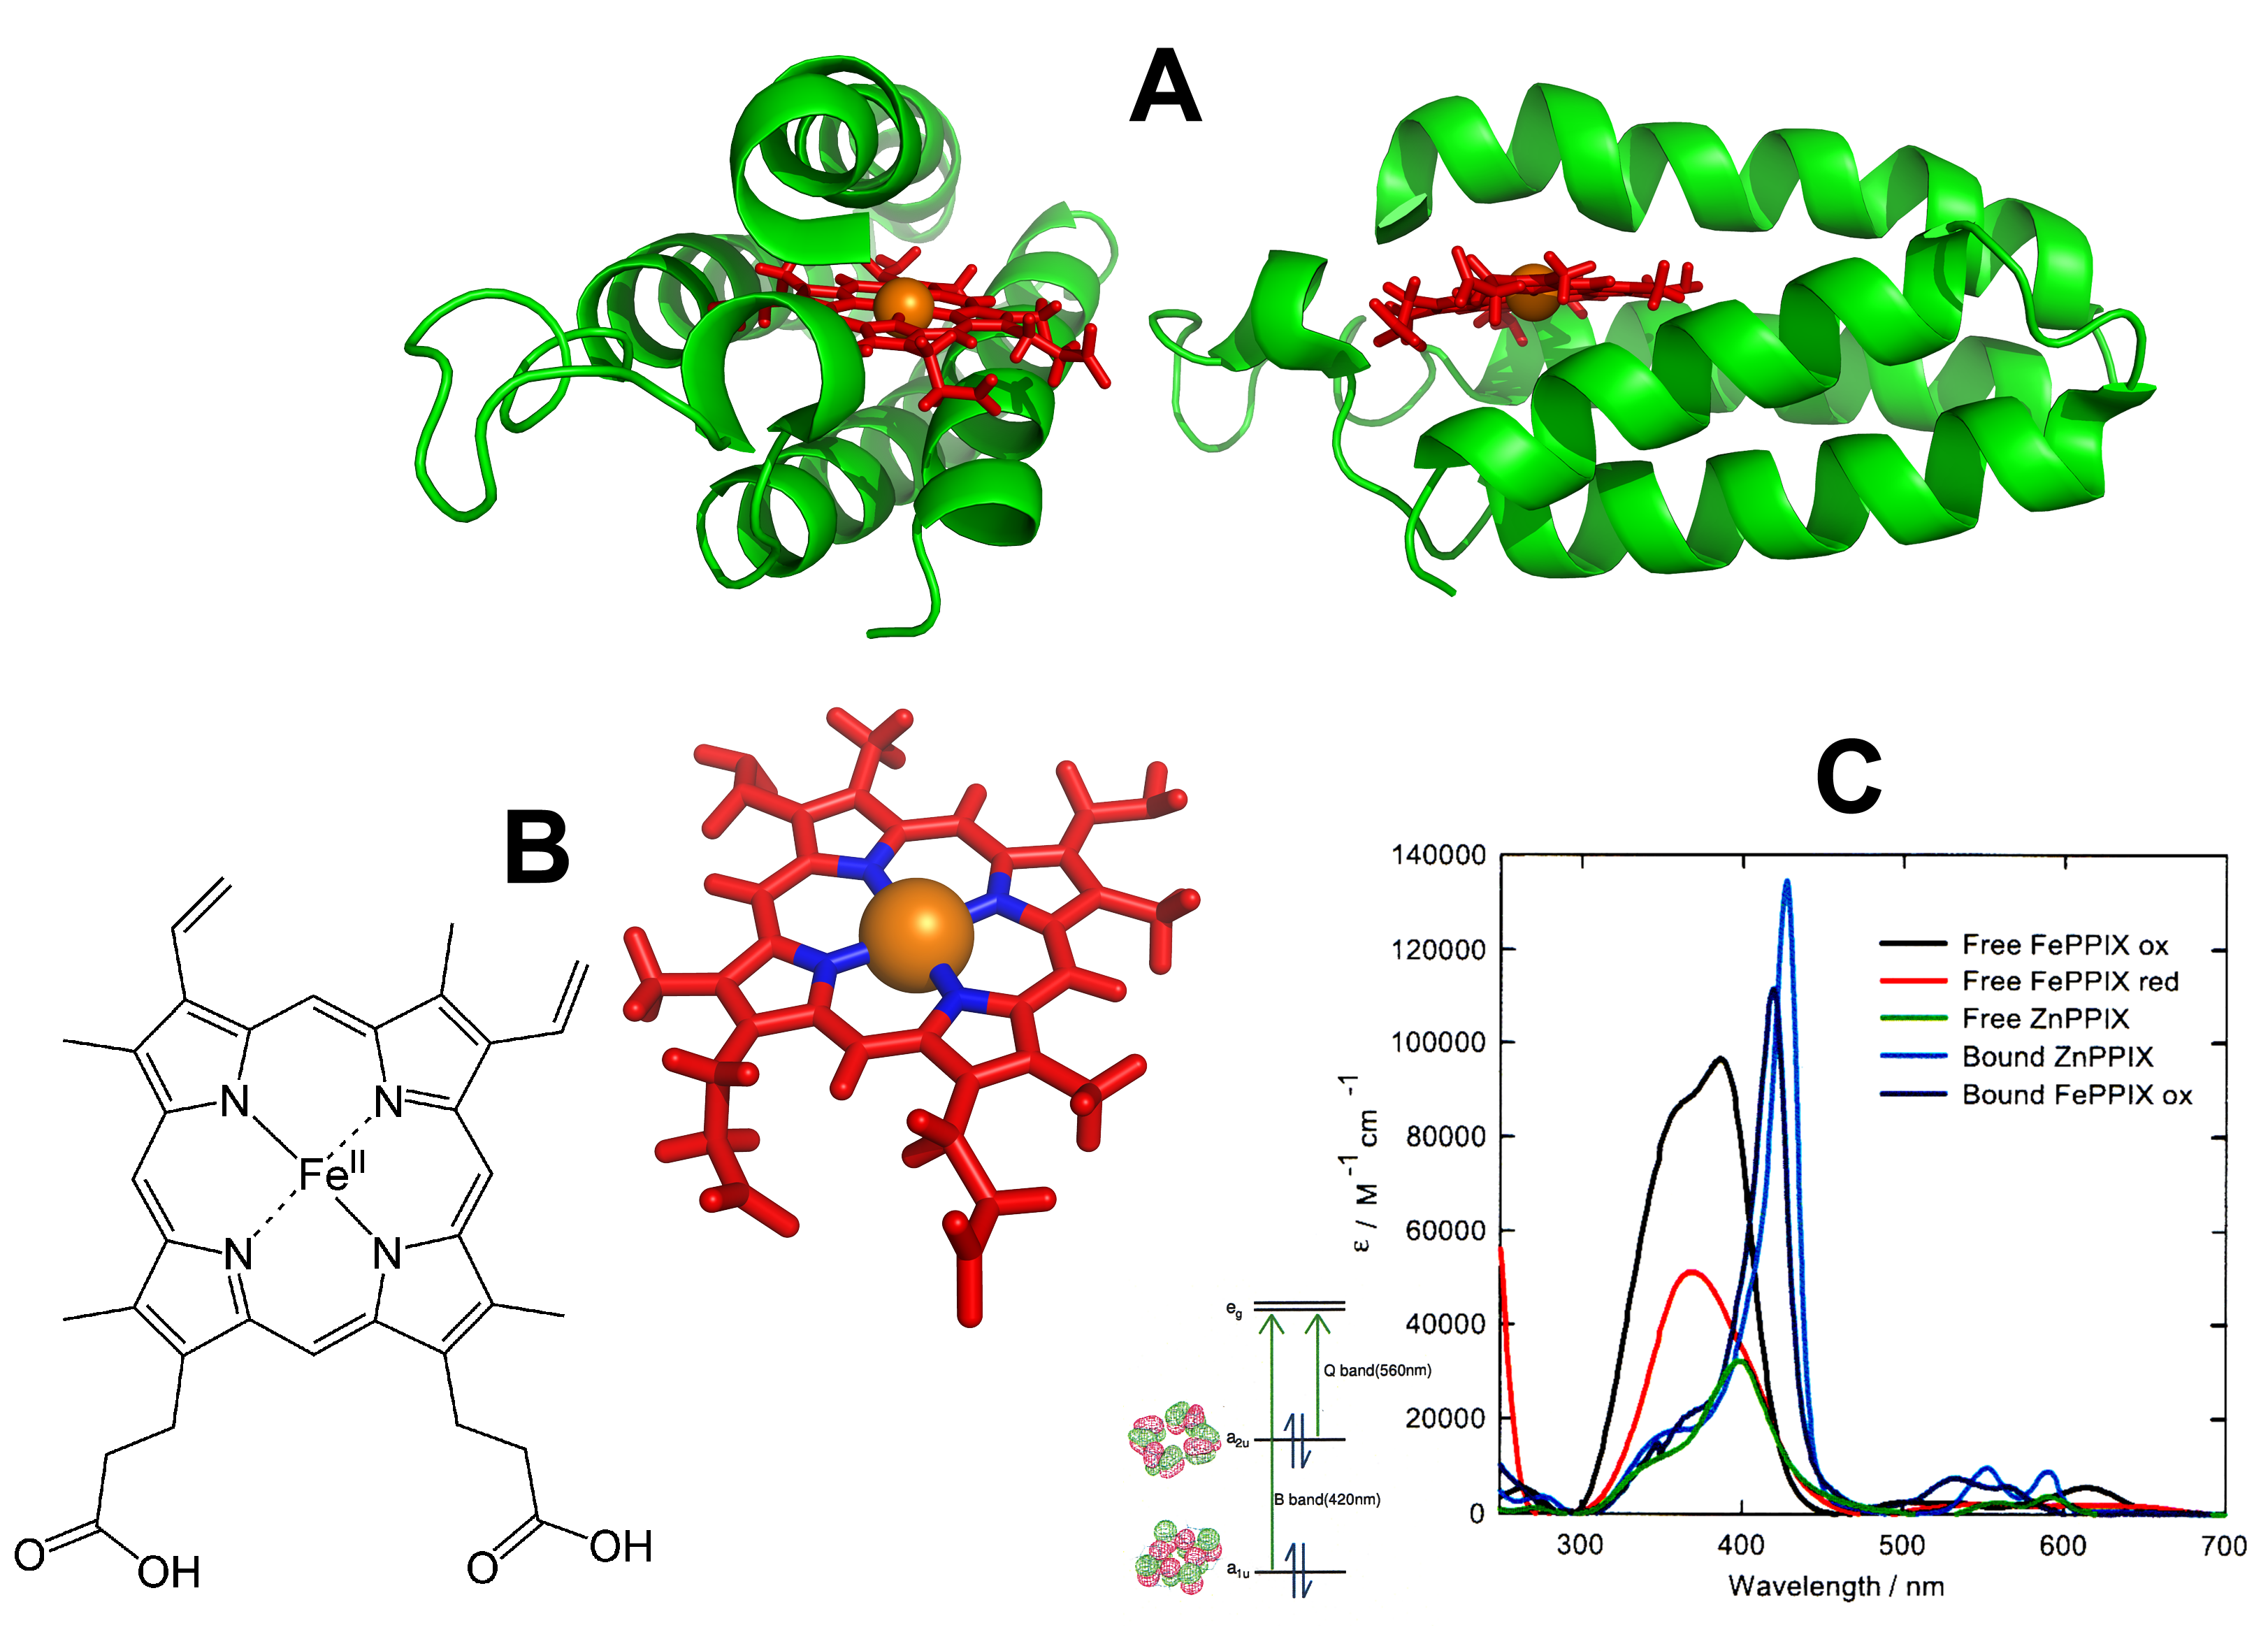
\includegraphics[width=137.4mm]{Images/haemStructure.png}
	\caption[Haem Structure]{A fancy image.}
	\label{fig:haemStructure}
\end{figure}
\end{verbatim}

\vspace{2ex}

\begin{figure}[!th]
	\centering
	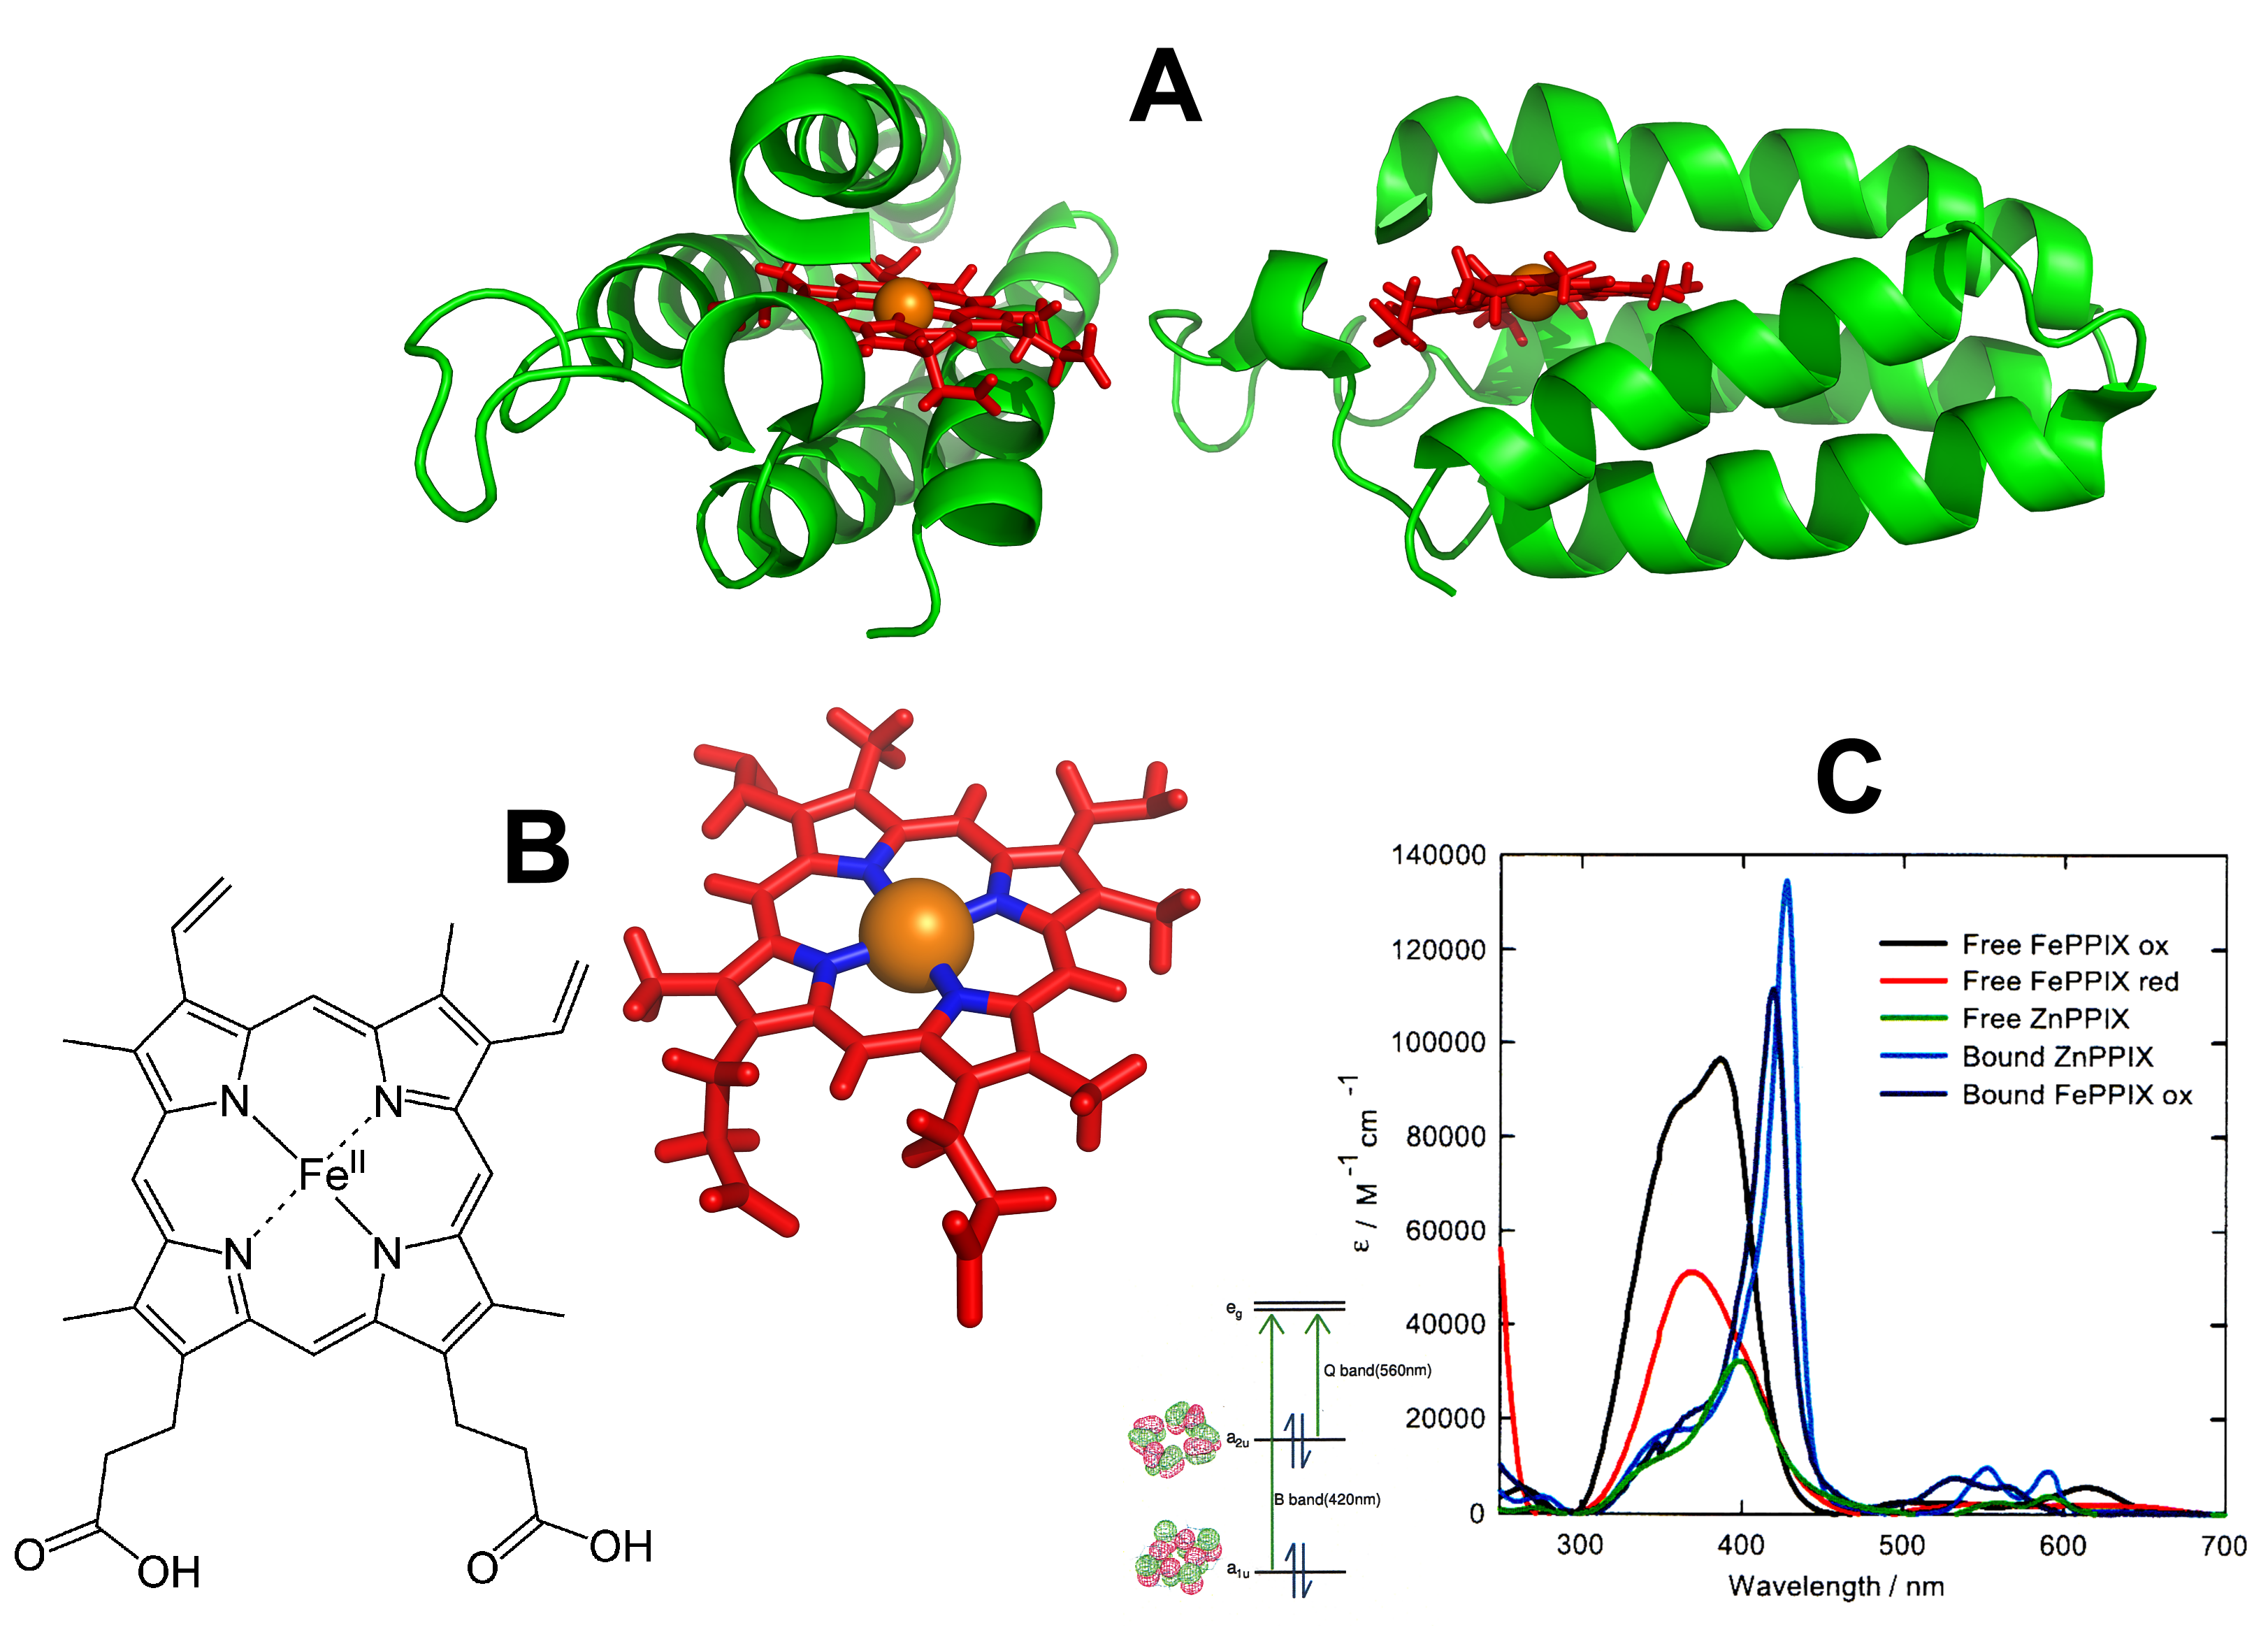
\includegraphics[width=137.4mm]{Images/haemStructure.png}
	\caption[Haem Structure]{A fancy image from Chris' Thesis.}
	\label{fig:haemStructure}
\end{figure}

In this example the command {\textbackslash}includegraphics tells LaTeX to look in the directory `Images' and incorporate the file called `haemStructure.png' into the final document while setting the width to 137.4mm.  This command can be used to resize a graphical file using the height or width parameter as shown. You must specify the units which can be pt, ex, em, mm, cm and so on. LaTeX recognises a very wide variety of standard units and graphics formats. The command is part of the graphicx package and so in the preamble you must include the command {\textbackslash}usepackage\{graphicx\}.

Many packages have been written to provide new commands. For example the `subfigure' package enables you to place separate images or files in the same figure side by side while giving them their own label. However, in this document we only concentrate on the very basics.

\section{Floating Environments}

Both tables and figures are examples of a `floating environments' which means LaTeX decides where to put them. 

The mysterious [!tbh] letters give guidance to LaTeX about roughly where the figure or table is  allowed to be, but in general they can move a long way from where you position them within your text file.  The letters in the square bracket can be t, h or b which stand for top, here or bottom.  If you don't specify any letters LaTeX defaults to [t].

LaTeX will always preserve the order in which figures appear.  If it cannot find a type setting solution, then it may move the float to it's own page, and combine it with other figures. If it still can't fit that in for some reason then it moves the float to the end of the document.  This has the effect of pushing all the remaining floating environments to the end of the document also.

The exclamation mark instructs LaTeX to ``try harder'' at putting the float where you told it to. Often you must play around to ensure the float positioning is acceptable, but usually this can be achieved by stretching or shrinking the image slightly using the size parameter, re-ordering text, judicial applications of the {\textbackslash}pagebreak command or by shouting loudly and slapping the computer monitor about. Note that it is better to resize the image using the original program that was used to create the image. Also using vector graphics can assist be useful (e.g. eps files) because they are designed to scale better.
\include{Chapters/Maths Equations}
\include{Chapters/Chemical Equations}
\chapter{Organising Your Files}
One of the drawbacks of word is that the figures and tables are included within the document which becomes very very clunky quite quickly and once it reaches around 100Mb it becomes unwieldy and hard to export. One of that advantages of LaTeX is that the files are all text files and so are very light on resources and are easy to email around the place.

However, sometimes it can be difficult to navigate through a single text file, so if you had a huge document then it becomes difficult to find your way around.  One way of circumnavigating this problem is to break the file up into smaller files. As long as LaTeX knows where to look you can have a file for each logical sub-division of your document.

Therefore it is worth spending a bit of time at the beginning of a large project deciding how you wish to break up your LaTex Files and organise them neatly and tidily.  You can then tell LaTex where to look for the files using the following command:

\vspace*{2ex}
{\textbackslash}include\{fileName\}
\vspace*{2ex}

\pagebreak
\section{Linking a File}
We are now going to copy part of the tutorial file into a separate files and link it the main file.  Because this could go wrong it is sensible to back up tutorial.tex as something else. So save a copy called `tutorialOriginal.tex' for safe keeping. Then follow the following instructions.

\begin{enumerate}
\item Create a new file called MyFirstPage.tex
\item Select and Cut out the first chapter of Tutorial.Tex
\item Paste the first chapter into MyFirstPage.tex
\item Save both tutorial.tex and MyFirstPage.tex
\item Then add {\textbackslash}include\{MyFirstPage\} in tutorial.tex where the text used to be before you cut it out. We don't need to add the `.tex' because LaTeX can only include `.tex' files.
\item compile tutorial.tex and view the PDF
\end{enumerate}

The final PDF should look exactly the same as it was! except we now have a separate file for one of the chapters.

\pagebreak
\section{Creating A Class File}
We can also save our preamble in a separate file called a class file. This makes your main document much easier to understand.  To make it work we need to use the {\textbackslash}LoadClass\{\} command as follows: 

\begin{enumerate}
\item Create another new file and save it as TutorialStyle.cls
\item Copy the preamble of tutorial.tex into the new file. Starting with the {\textbackslash}documentclass{} command and copy right up to, but not including, the {\textbackslash}begin{document} command. Delete the preamble in the original document.
\item Save TutorialStyle.cls and tutorial.tex
\item Modify the first line of TutorialStyle.cls by replacing the word `document' with the word `Load'.
\item Add a new first line of tutorial.tex to use your new style class {\textbackslash}documentclass\{TutorialStyle\}
\item Save both files.
\end{enumerate}

\subsection{Sanity Check}

The first line of TutorialStyle.cls should now be:

\begin{verbatim}
\LoadClass[12pt, oneside, a4paper]{book}
\end{verbatim}
\vspace{2ex}

The first line of tutorial.tex should be:

\begin{verbatim}
\documentClass{TutorialStyle}
\end{verbatim}
\vspace{2ex}

We have just created what is called a style file. You can use this style file as a generic preamble for other documents as well. Compile tutorial.tex.  Nothing should have changed in the final PDF.


\pagebreak
\section{The Structure of this Document}

Lets now look at how I've organised this document. It is identical to my thesis because it started out life as my thesis. I usurped the structure and simply replaced the headings and content to make a kind of reference manual for this introductory course. This document therefore is three things:

\begin{enumerate}
\item An example thesis structure to work from.
\item The LaTeX files which were used to create it can be used as a template for a thesis.
\item It is also a convenient introductory latex manual!
\end{enumerate}

\vspace*{2ex}
Groovy huh?

\section{The Master File}

There is a master file where LaTeX begins the compilation procedure. This contains the {\textbackslash}documentclass command needed to set the ball rolling. Within the file there are a series of {\textbackslash}include\{\} commands, one for each Chapter, which tell LaTeX where to find the files containing each chapter.

The subfiles cannot be compiled on their own because they do not contain the {\textbackslash}documentclass, {\textbackslash}begin\{document\} or {\textbackslash}end\{document\} commands. Lets us look in more detail at the master file and we will learn some new LaTeX commands.

\singlespacing
\pagebreak
\begin{verbatim}
\documentclass{Style/LatexCourseStyle}

\begin{document}
\setcounter{secnumdepth}{2}
\setcounter{tocdepth}{1}

\frontmatter
\onehalfspacing
\thispagestyle{empty}

\begin{center}
\vspace*{\stretch{1}}

\hrule height 2pt
\vspace*{2ex}
{\Huge\textbf{Towards the Ability to Make Super Duper LaTeX Documents}\par}
\vspace*{2ex}
\hrule height 2pt
\vspace*{10ex}
{
\includegraphics[height=40mm]{Images/UnivShield}\par}
\vspace*{10ex}
{\large\textbf{Christopher~James~Forman}\par}
\vspace*{2ex}
{\large{Department Of Chemistry}\par}
\vspace*{2ex}
{\large{University of Cambridge}\par}
\vspace*{5ex}
{\large{This dissertation is submitted for the degree of \textit{Doctor of Philosophy}}\par}
\vspace*{5ex}
{\large{\today}\par}

\vspace*{\stretch{2}}
\end{center}
\chapter*{Declaration}

\vfill

This dissertation is the result of my own work and includes nothing which is the outcome of work done in collaboration except where specifically indicated in the text. It is not substantially the same as any that I have submitted for a degree or diploma or other qualification at any other University and no part has already been, or is concurrently being, submitted for any degree, diploma, or other qualification. It does not exceed 60,000 words, including tables, footnotes, bibliography and appendices.\par

\vspace{10ex}

\begin{flushright}
Signature: \rule[0pt]{60mm}{0.5pt}

\vspace{5ex}

Date: \rule[0pt]{60mm}{0.5pt}
\end{flushright}

\vfill
\chapter*{Acknowledgments}
\subsection*{Family}
Mum. Dad. Pet Dog.

\subsection*{Scientific Collaborations}
Dr A.N.Other at uni of blah for samples and instrument time etc. My Amazing Lab Chums.

\subsection*{Scientific Support}
My amazing lab chums.

\subsection*{General Assistance}
Cleaner, My amazing lab chums.

\subsection*{Financial Support}
Bank, Tax payer. My amazing lab chums.

\subsection*{Moral Support}
My Amazing Lab chums.

\subsection*{Academic Inspiration}
Netwon, My super. My Amazing Lab Chums.

\subsection*{Everyone else}
My Amazing Lab Chums.

\chapter*{Summary}
This document is a handbook for introducing you to LaTeX. It contains a bit of background about the history and philosophy of LaTeX.  However, it concentrates on providing a guided practical introduction to the basic techniques such as 
\begin{itemize}
\item Lists
\item Mathematical and chemical equations
\item Tables
\item Figures
\item Chapters and Sections
\item Linking to other files in large documents
\item Referencing
\end{itemize}

The handbook is also presented in the style of a thesis. This means that source files provided on the introductory course and available from the department web page are a convenient template for a thesis.

More details on specific aspects of LaTeX can be found at the departmental LaTeX page which can be found here:

 http://www-ch-int.ch.private.cam.ac.uk/latex/about

\chapter*{Abbreviations}

\begin{longtable}{r >{\rule{0pt}{3ex}}l<{\rule[-1.5ex]{0pt}{0pt}}}
ADP & Adenosine Diphosphate\\
(nc/c)AFM & (non-contact/conducting) Atomic Force Microscopy\\
ATP & Adenosine Triphosphate \\
\end{longtable}
\tableofcontents
\listoftables
\listoffigures

\mainmatter
\renewcommand{\sectionmark}[1]{\markright{\thesection \ #1}{}}
\chapter{Overview}
\label{chap:overview}
\section{LaTeX: The answer to everything.}
LaTeX is typsetting program that takes an input file of marked up text and then, with a user defined set of rules, typesets a beautifully crafted output file that can be easily printed (e.g. a pdf). 

\subsection{Advantages}

The advantages of this method are manifold:

\begin{itemize}

\item Use any text editor to view the source document.
\item More time can be spent working on the content and not worrying about how text or figures interact in the layout until later on.
\item LaTeX uses consistent rules throughout a document
\item LaTeX sorts out basic typesetting automatically
\item Changes can be introduced globally with very little effort
\item Document structure is explicit
\item Documents can be professionally typeset and look great
\item You are forced to structure your documents correctly.
\item Mathematical equations, like $E=mc^2$ or $\imath\hbar\frac{\partial}{\partial t}\Phi (x, t) = \hat{H}\Phi (x, t)$ can be produced almost as fast as typing (if you know the commands!).
\end{itemize}

\subsection{Disadvantages}
The disadvanatges of this method are also manifold:
\begin{itemize}
\item You don't see the output as you go.
\item Steep learning curve.
\item Documents are harder to edit by a second author (unless they are adept at LaTeX too). This can be mitigated using version control, which makes group authoring processes superior to word.
\item The program never works quite the way you want it to and learning how to influence it can be problematic and subtle.
\item Although intended to save work the principle of 'conservation of work' means that you simply transform problems associated with WYSISYG approaches to problems associated with WYSIWYM approaches!
\item You can go blind trying to determine the difference between wiggly and smooth brackets if your editors font isn't large enough.
\end{itemize}

\subsection{On balance?}
If it's so rubbish, why use LaTeX?

\begin{itemize}
\item Large documents are much more easily handled. 
\item In general it is quicker to debug a LaTeX document than typeset an entire thesis manually. 
\item Technical information such as tables, equations and figures are integrated much more smoothly than with word.
\end{itemize}

\section{How does it work?}

The raw text is interspersed with commands, preceded by a \textbackslash, which tell LaTeX what to do with the text. For example you can \textbf{make it bold}, \emph{italic}, or \underline{underlined} with the commands {\textbackslash}textbf\{\}, {\textbackslash}emph\{\} or {\textbackslash}underlined\{\}. More on commands in a moment...



\chapter{My First Page}

\section{The Very Beginning}
The very simplest LaTeX document might look like this:

\begin{verbatim}
\documentclass[a4paper,12pt]{article}
\begin{document}
Hello World.
\end{document}
\end{verbatim}

\pagebreak
\thispagestyle{empty}
Hello World.
\pagebreak
\subsection{Break Down}
What's all the gobbledegook around my simple message???

In LaTeX we intersperse text and commands.  Commands are preceded by a \textbackslash. For example the first line in a LaTeX document \underline{\textbf{\emph{must}}} be:

\begin{verbatim}
\documentclass[options]{class}
\end{verbatim}

Where the word ''class'' may be substituted for one of many things such as: article, proc, minimal, report, book, letter, memoir, slides, beamer.

Similarly, and completely generally in LaTeX speak, the square brackets denote the existence of optional parameters. Each individual command can take its own parameters and for the ''{\textbackslash}documentclass'' command there are options for controlling font size, font family, landscape, oneside, twosided, page size and so on. These options will persist throughout the entire document. For example the document class command for this document, (which is likely to be like the one you would use for a thesis), would be:

\begin{verbatim}
\documentclass[12pt, oneside, a4paper]{book}
\end{verbatim}

Other options include:

\begin{itemize}
\item {10pt, 11pt, 12pt (default is 10pt).}
\item {letterpaper, legalpaper, a4paper, executivepaper, a5paper, b5paper}
\end{itemize}
and so on.

\pagebreak
\section{Can I start typing please?}

After we have set up the document we can start actual work on our document. So we must tell LaTeX that what follows is to be interpreted as a document.  The command {\textbackslash}begin can take many different parameters and is a command to enter what is known, in LaTeX speak, as 'an environment'. Thus the commands:
\begin{verbatim}
\begin{document}

\end{document}
\end{verbatim}

tells LaTeX to enter and leave the document environment, and thus constitute the outer limits of our document file. Other environments include the equation environment, the itemize environment, the figure environment and so on. These will be encountered in due course.

Every part of the LaTeX file is therefore within an environment of specific type and the content within each environment consists of commands or text.

That's basically it.

So let's get on with it shall we...

\pagebreak
\section{The ground rules}
\begin{quote}
Hold on, hold on, hold on my son.

First the lessons.

Then the fun!
\end{quote}
Dr Seuss.

\subsection{Spaces}
Whitespace characters, such as blank or tab, are treated uniformly as space by LaTeX. Several consecutive whitespace characters are treated as one single space. Whitespace at the start of a line is generally ignored, and a single line break is treated as whitespace. An empty line between two lines of text defines the end of a paragraph. Several empty lines are treated the same as one empty line. The text below is an example.

\begin{verbatim}
It does not matter whether you
enter one or several             spaces
after a word. The final result will be typeset beautifully
according    to     precise rules.




An empty line starts a new
paragraph. Note the indentation on the first line of the paragraph, 
except at the beginning of the section. 
\end{verbatim}

\vspace*{2ex}
\vspace*{2ex}

It does not matter whether you
enter one or several             spaces
after a word. The final result will be typeset beautifully
according    to     specific rules.




An empty line starts a new
paragraph. Note the indentation on the first line of the paragraph, except at the beginning of the section. 

\pagebreak
\subsection{Special Characters}
The symbols 

\# \$ \% \textasciicircum{} \& \_ \{ \} \~{} \textbackslash

are reserved characters that either have a special meaning under LaTeX or are unavailable in all the fonts. If you enter them directly in your text, they will normally not print, but rather make LaTeX do strange things.

To overide the special meanings of these symbols and allow them to produced within your text you may use the following sequences:
\begin{verbatim}
\# \$ \% \textasciicircum{} \& \_ \{ \} \~{} \textbackslash
\end{verbatim}

Other symbols and many more can be printed with special commands in mathematical formulae or as accents.

The backslash character '\textbackslash' cannot be entered by adding another backslash in front of it ( \textbackslash\textbackslash); because this sequence means ''linebreak''.

The command \textbackslash\~{}\{\} produces a tilde which is placed over the next letter. For example \textbackslash\~{}\{n\} gives \~{n}. To produce just the character \~{}, use \textbackslash\~{}\{\} which places a \~{} over an empty box.

Similarly, the command \textbackslash\textasciicircum{} produces a hat over the next character, for example \textbackslash\textasciicircum\{o\} produces \^{o}.

\pagebreak
\section{Preamble}
After the {\textbackslash}documentclass command we add ''preamble''. Here we load special features that we will use throughout our document to expand on the basic capabilities of LaTex. These are contained in units called ''packages'' which we can tell our LaTeX compiler to download by using the command ''{\textbackslash}include\{packageName\}''. 

There are many repositories of such packages on the web. Your compiler generally knows where to look and most standard packages are included with any install. For example, to include a special set of typesetting instructions to handle chemical equations we can grow our simple document with a single command like this:

\begin{verbatim}
\documentclass[a4paper,12pt]{article}
\usepackage[version=3]{mhchem}
\begin{document}
Hello World!

We all need \ce{H2O}.

I'm less fussed about \ce{^{235}_{92}U+}.

\end{document}
\end{verbatim}

\vspace{2ex}

\pagebreak
\thispagestyle{empty}
Hello World!

We all need \ce{H2O}.

I'm less fussed about \ce{^{235}_{92}U+}.
\pagebreak

Here we have loaded a package called: "`mhchem"' which took the option ''[version=3]''. This is a package for drawing chemical equations easily and it has it's own instruction manual which you can follow easily. It is included in the bundle of files for this course.

Other things we can do in the premable within LaTeX are to redefine existing commands or create our own personal commands. These can be stored in a file called the 'style file' which we can load at the beginning of our document, in place of our documentclass. More about this later on...


\subsection{Comments}
It is often useful to comment your LaTeX documents. You can leave yourself amusing, sarcastic messages that won't get printed out in the final document. Use this to make your own notes as the course progresses.

To get a comment use the \% command, which tells LaTeX to ignore the rest of the line, the line break and all the white space at the beginning of the next line, for example, we may add to our continually evolving document...

\begin{verbatim}
\documentclass[a4paper,12pt]{article}
\usepackage[version=3]{mhchem}
\begin{document}
Hello World!

%All humans need water and I would like 
%to include this concept in my arguments.
We all need \ce{H2O}.

%Uranium 235 is toxic, which is why I don't want to consume it... 
I'm less fussed about \ce{^{235}_{92}U+}.

\end{document}
\end{verbatim}

\vspace{4ex}
Hello World!

%All humans need water and I would like to include this concept in my arguments.
We all need \ce{H2O}.

%Uranium 235 is toxic, which is why I don't want to consume it... 
I'm less fussed about \ce{^{235}_{92}U+}.

\pagebreak
\section{Compiling}
Once the document is finished you can compile it. Your compiler will depend on the platform that you use. In the PWF we are using winEDT to edit the documents (a LaTeX front end) and texlive2008 which is the compiler itself. I use MiKTex and the front end texCenter.  There is no need to use a front end. If you prefer you can use a simple text editor and a command line.

the recommended distributions are:
\begin{itemize}
\item MiKTeX or TeX Live for Windows
\item TeX Live for Unix/Linux
\item MacTeX or TeX Live for Mac OS.
\end{itemize}

Once you have installed your software and got it working, written your source code and tried to compile it, there will nearly always be something wrong with your file. 

Any errors will be highlighted in the console window or error output box of your front end.  Some front ends dump the running commentary which LaTeX produces into a text file for easy reading afterwards.

In a compile attempt (successful or otherwise) LaTeX may produce the following files:

projectname.aux

projectname.bbl

projectname.lof

projectname.lot

projectname.txt

projectname.toc

projectname.dvi

These are interim files (toc= table of contents, bbl = bibliography etc). To be honest I have no idea what half of these things contain.  You only need the .tex file and a compiler with the right packages installed to produce them again.

Some versions of LaTeX only produce DVI files and you then need to convert the dvi file to a PDF or download a dvi viewer. You can also convert DVI files to PS files and then view them.  The good thing about front ends is that you can set them up to produce PDFs directly.

OK. So we have now produced a silly document but we understand it.  Now lets get on with learning how to make our own documents.



\chapter{Lists}
Lists are great.  The command {\textbackslash}begin\{\} can be used to enter a list environment.  For example:

\begin{verbatim}
\begin{itemize}
\item cat
\item dog
\item horse
\end{itemize}
\end{verbatim}

Produces:

\begin{itemize}
\item cat
\item dog
\item horse
\end{itemize}

\pagebreak
We can also replace the bullet points with numbers using the enumerate keyword.

\begin{verbatim}
\begin{enumerate}
\item cat
\item dog
\item horse
\end{enumerate}
\end{verbatim}

\begin{enumerate}
\item cat
\item dog
\item horse
\end{enumerate}

\pagebreak
and we can use the description keyword which does this:
\begin{verbatim}
\begin{description}
\item[Cat] a lovely furry creature with a cute nose and whiskers.
\item[Dog] Another furry creature that smells rather well; 
           its olfactory power stems from its nasal dampness.
\item [Horse] A large stinky creature with sideways facing eyes.
\end{description}
\end{verbatim}

\begin{description}
\item[Cat] a lovely furry creature with a cute nose and whiskers.
\item[Dog] Another furry creature that smells rather well; its olfactory power stems from its nasal dampness.
\item [Horse] A large stinky creature with sideways facing eyes.
\end{description}
\chapter{Maths Equations}

\section{Producing Beautiful Looking Mathematics}

One of the best features about LaTeX is `maths mode'.  For example the schrodinger equation can be produced as follows:

\vspace*{2ex}

\begin{center}
\begin{math}
\imath\hbar\frac{\partial}{\partial t}\Phi (x, t) = \hat{H}\Phi (x, t)
\end{math}
\end{center}

\vspace*{2ex}

\begin{verbatim}
\begin{math}
\imath\hbar\frac{\partial}{\partial t}\Phi(x,t)=\hat{H}\Phi(x,t)
\end{math}
\end{verbatim}

There are a number of ways to switch on maths mode.  The first, as above, is with the {\textbackslash}begin\{math\} environment. You can also enter mathmode inline using the \$ symbol. For example typing in \$y=ax\textasciicircum{}2+bx+c\$ yields $y=ax^2+bx+c$.  Another way is to enter the equation environment which enables you to number equations so you can then refer to them later in the text.

\begin{equation}
y(t)= \sin \left(\frac{{\alpha}t}{2\pi} + \phi_0\right)
\label{eqn:MadeUpNonsense}
\end{equation}

\vspace*{2ex}
\begin{verbatim}
\begin{equation}
y(t)= \sin \left(\frac{{\alpha}t}{2\pi} + \phi_0\right)
\end{equation}
\end{verbatim}.

\section{Basic Maths Mode}
Once in maths mode there is a kind of text based code for writing down your equations.  Here are the most basic symbols to get you going.
\begin{center}
\begin{tabular}{cc}
\toprule
Final Result & LaTeX Code \\
\cmidrule(){1-2}
$a+b$ & a+b \\
$a-b$ & a-b \\
$ab$ & ab \\
$a*b$ & a*b \\
$a \times b$ & a {\textbackslash}times b \\
$a \cdot b$ & a {\textbackslash}cdot b \\
$\frac{a}{b}$ & {\textbackslash}frac\{a\}\{b\} \\ 
$a^b$ & a\textasciicircum{}b \\
$a_b$ & a\_b \\
$\sin a$ & {\textbackslash}sin a  (same for cos, tan)\\
$ sin a$ & sin a \\
$\sqrt{a}$ & {\textbackslash}sqrt\{a\} \\
$\left( a \right) $ & {\textbackslash}left( a {\textbackslash}right)\\ 
$\left[ a \right]$ & {\textbackslash}left[ a {\textbackslash}right]\\ 
$\alpha$ & {\textbackslash}alpha \\
$\pi$ & {\textbackslash}pi \\
\bottomrule
\end{tabular}
\end{center}

A full treatise on maths mode is not practical here. There are lots of online tutorials and summaries of symbols. It just takes a bit of practice and you can build up equations really easily. It's straight forward to learn new stuff once you've done it a few times.

\pagebreak
\section{Equation Arrays}
Sometimes you need to arrange several equations vertically, referencing individual lines separately and aligning the equations on the $=$ sign. This can be achieved with equation arrays as follows:

\begin{eqnarray}
A\left( x\right) & = & \frac{x^2+2x+1}{x+1} \\
& = & \frac{\left(x+1\right)\left(x+1\right)}{x+1} \nonumber\\
& = & x+1 \nonumber\\
B(x,t) & = & \frac{e^{\left(\imath\omega_0 t + kx\right)}}{4\pi\epsilon_0}
\end{eqnarray}

\begin{verbatim}
\begin{eqnarray}
A\left( x\right) & = & \frac{x^2+2x+1}{1+x} \\
& = & \frac{\left(x+1\right)\left(x+1\right)}{1+x} \nonumber\\
& = & x+1 \nonumber\\
B(x,t) & = & \frac{e^{\left(\imath\omega_0 t + kx\right)}}{4\pi\epsilon_0}
\end{eqnarray}
\end{verbatim}

\begin{itemize}
\item Note the \& symbols. This tells LaTeX where to align the equations. There must be the same number of \& symbols in each line.
\item Note the \textbackslash\textbackslash ~at the end of each line except the last one. This symbol tells LaTeX to add another row in the array.  If you put it on the last line you get an empty row at the bottom of the array.
\item Note the {\textbackslash}nonumber command which suppresses line numbering for that line.
\item Note that equation number carries on from equation \ref{eqn:MadeUpNonsense} in the previous section.
\end{itemize}

\section{Maths Packages}

Maths mode comes as standard in LaTeX, however you can download packages that buff up your maths symbol set. For example neat vector notation comes in the package `vector'. e.g. {\textbackslash}uuvec\{T\} yields $\uuvec{T}$.

\begin{verbatim}
\usepackage{amssymb}
\usepackage{amsmath}
\usepackage{vector}
\end{verbatim}


\chapter{Chemical Equations}
The mhchem package means you can do basic stuff very easily using {\textbackslash}ce\{\}. For example:

\vspace{2ex}
\begin{verbatim}
\ce{CO2 + C -> 2CO}
\ce{CO2 + C <- 2CO}
\ce{CO2 + C <=> 2CO}
\ce{A-B=C#D\sbond E\dbond F\tbond G}
\end{verbatim}
\vspace{2ex}
\begin{center}
\ce{CO2 + C -> 2CO}

\ce{CO2 + C <- 2CO}

\ce{CO2 + C <=> 2CO}

\ce{A-B=C#D\sbond E\dbond F\tbond G}
\end{center}

\vspace{2ex}
You can also use math mode within chemical equations.
\vspace{2ex}

\begin{center}
\ce{$x\,$ Na(NH4)HPO4 ->[\Delta] (NaPO3)_{$x$} + $x\,$ NH3 ^ + $x\,$ H2O}
\end{center}

\begin{verbatim}
\ce{$x\,$ Na(NH4)HPO4 ->[\Delta](NaPO3)_{$x$} + $x\,$ NH3 ^ + $x\,$ H2O}
\end{verbatim}

And you can number chemical reactions as well by using the math mode equation environment.

\begin{equation}
\ce{CO2 + C <=> 2CO}
\end{equation}

\begin{verbatim}
\begin{equation}
\ce{CO2 + C <=> 2CO}
\end{equation}
\end{verbatim}

However, this will number mathematical and chemical equations using the same number system. There is a discussion in the mhchem pdf which shows you how to number chemical and mathematical equations independently. It's a bit complex and involves you creating your own type of environment... bit beyond the intro level of this course...
\chapter{Tables}
Tables are big business in Latex.  I use these packages to help me.

\begin{verbatim}
\usepackage{multirow}
\usepackage{booktabs}
\usepackage{dcolumn}
\end{verbatim}

Here's an example table

\begin{table}[!hb]
 \centering
	\begin{tabular}{@{}rccc@{~}r@{.}l*3{r@{.}l@{~}r@{.}l}D{.}{\cdot}{2,1}}
	\toprule
	\multicolumn{1}{c}{Fibre Type}
	& N 
	& M 
	&\multicolumn{3}{c}{$L_t$ (nm)}
	&\multicolumn{4}{c}{$R_t$ (nm)}
	&\multicolumn{4}{c}{$d_t$ (nm)}
	&\multicolumn{4}{c}{${\Delta}Z_t$ (nm)}
	&\multicolumn{1}{c}{~}\\
\cmidrule(lr){1-1}
\cmidrule(lr){2-2}
\cmidrule(lr){3-3}
\cmidrule(lr){4-6}
\cmidrule(lr){7-10}
\cmidrule(lr){11-14}
\cmidrule(lr){15-18}
  SS Twisted & 5 & 4 & 313 &\multicolumn{2}{c}{(122)} & 5&7 &(1&6)  & 5&4 &(1&0)  &  150&5 &(63&1) &\multicolumn{1}{c}{~} \\
  \multicolumn{19}{c}{~}\\
  %\cmidrule(lr){3-18}
  &
  &
 	&\multicolumn{3}{c}{$L_s$ (nm)} 
 	&\multicolumn{4}{c}{$R_s$ (nm)}
 	&\multicolumn{4}{c}{$W_s$ (nm)}
 	&\multicolumn{4}{c}{${\Delta}Z_s$ (nm)}
 	&\multicolumn{1}{c}{${\Delta}Z_{e}$ (nm)}\\
\cmidrule(lr){4-6}
\cmidrule(lr){7-10}
\cmidrule(lr){11-14}
\cmidrule(lr){15-18}
\cmidrule(lr){19-19}
  SS Spiral& 32 & 7 &123&(31&6)&11&4&(3&3)&11&1&(2&6)&32&9&(22&2)&26.9\\
  SSB Spiral& 64&18 &106&(22&9)&10&8&(2&7)&9&8&(1&8)&28&2&(8&1)&22.7\\
	%\midrule
  BSS Spiral&37 &19 &110&(44&9)&13&4&(3&0)&12&9&(1&8)&27&1&(9&1)&21.5\\
	%\midrule
  SSSB Spiral&26& 6 &104&(23&9)&13&3&(2&6)&16&4&(3&4)&29&9&(11&1)&22.5\\
	\bottomrule
	\end{tabular}	
	\caption[Basic Fibre Dimensions by TEM]{A funky table from my thesis.}
	\label{tab:BasicXSBFibreDimensionsTEM}
\end{table}

\pagebreak
Here's what the code looks like:
\begin{verbatim}
\begin{table}[!hb]
 \centering
	\begin{tabular}{@{}rccc@{~}r@{.}l*3{r@{.}l@{~}r@{.}l}D{.}{\cdot}{2,1}}
	\toprule
	\multicolumn{1}{c}{Fibre Type}
	& N 
	& M 
	&\multicolumn{3}{c}{$L_t$ (nm)}
	&\multicolumn{4}{c}{$R_t$ (nm)}
	&\multicolumn{4}{c}{$d_t$ (nm)}
	&\multicolumn{4}{c}{${\Delta}Z_t$ (nm)}
	&\multicolumn{1}{c}{~}\\
\cmidrule(lr){1-1}
\cmidrule(lr){2-2}
\cmidrule(lr){3-3}
\cmidrule(lr){4-6}
\cmidrule(lr){7-10}
\cmidrule(lr){11-14}
\cmidrule(lr){15-18}
  SS Twisted & 5 & 4 & 313 &\multicolumn{2}{c}{(122)} & 5&7 &(1&6)  & 5&4 &(1&0)  &  150&5 &(63&1) &\multicolumn{1}{c}{~} \\
  \multicolumn{19}{c}{~}\\
  %\cmidrule(lr){3-18}
  &
  &
 	&\multicolumn{3}{c}{$L_s$ (nm)} 
 	&\multicolumn{4}{c}{$R_s$ (nm)}
 	&\multicolumn{4}{c}{$W_s$ (nm)}
 	&\multicolumn{4}{c}{${\Delta}Z_s$ (nm)}
 	&\multicolumn{1}{c}{${\Delta}Z_{e}$ (nm)}\\
\cmidrule(lr){4-6}
\cmidrule(lr){7-10}
\cmidrule(lr){11-14}
\cmidrule(lr){15-18}
\cmidrule(lr){19-19}
  SS Spiral& 32 & 7 &123&(31&6)&11&4&(3&3)&11&1&(2&6)&32&9&(22&2)&26.9\\
  SSB Spiral& 64&18 &106&(22&9)&10&8&(2&7)&9&8&(1&8)&28&2&(8&1)&22.7\\
	%\midrule
  BSS Spiral&37 &19 &110&(44&9)&13&4&(3&0)&12&9&(1&8)&27&1&(9&1)&21.5\\
	%\midrule
  SSSB Spiral&26& 6 &104&(23&9)&13&3&(2&6)&16&4&(3&4)&29&9&(11&1)&22.5\\
	\bottomrule
	\end{tabular}	
	\caption[Basic Fibre Dimensions by TEM]{A funky table from my thesis.}
	\label{tab:BasicXSBFibreDimensionsTEM}
\end{table}
\end{verbatim}

\pagebreak

\section{Tables Made Easy}
Here is a simple table followed by the code that produced it.

\begin{center}
\begin{tabular}{lcr}
anchovy & banana & carrot \\
dog & apple & fennel \\
goat & strawberry & potato
\end{tabular}

\vspace*{2ex}

\begin{verbatim}
\begin{tabular}{lcr}
anchovy & banana & carrot \\
dog & apple & fennel \\
goat & strawberry & potato
\end{tabular}
\end{verbatim}
\end{center}

\vspace*{2ex}

The tabular environment is a special case of the ''array'' environment for distributing content uniformly across a region of the page.  This ability has already been exploited to align mathematical equations. For now though look at the first line.

\vspace*{2ex}

\begin{verbatim}
\begin{tabular}{lcr}
\end{verbatim}

\vspace*{2ex}

This command tells LaTeX to enter the tabular environment. The letters l, c and r in the curly braces tell LaTeX to create a table with three columns in which the first column is left justified, the second column is centered and the third column is right justified. Lets add a fourth column and this time center justify all the columns.

\begin{center}
\begin{tabular}{cccc}
anchovy & banana & carrot & Johnny\\
dog & apple & fennel & Pete\\
goat & strawberry & potato &
\end{tabular}

\vspace*{2ex}

\begin{verbatim}
\begin{tabular}{cccc}
anchovy & banana & carrot & Johnny\\
dog & apple & fennel & Pete\\
goat & strawberry & potato &
\end{tabular}
\end{verbatim}
\end{center}

\vspace*{2ex}

Each row in the table is a list of items separated by the {\&} symbol. The end of each row is denoted by \textbackslash\textbackslash.  The last row in the table doesn't have a \textbackslash\textbackslash. You do not have to have data between the ampersands but you must have the right number of ampersands to match the number of columns that LaTeX is expecting.

\subsection{Adding Borders To Tables}
\label{sec:vertLines}
Tables should never have vertical lines. No professionally typeset table contains vertical lines. Do not put vertical lines in your tables. That said it is easy to do.

\begin{center}
\begin{tabular}{|c|c|c|c|}
anchovy & banana & carrot & Johnny\\
dog & apple & fennel & Pete\\
goat & strawberry & potato &
\end{tabular}

\vspace*{2ex}

\begin{verbatim}
\begin{tabular}{|c|c|c|c|}
anchovy & banana & carrot & Johnny\\
dog & apple & fennel & Pete\\
goat & strawberry & potato &
\end{tabular}
\end{verbatim}
\end{center}

\vspace*{2ex}

Tables should have neatly headed columns with the heading for each field separated from the data by horizontal lines. The {\textbackslash}toprule, {\textbackslash}cmidrule{} and {\textbackslash}bottomrule commands from the booktabs package are useful for controlling horizontal lines.

\begin{center}
\begin{tabular}{cccc}
\toprule
Ingredient 1 & Ingredient 2 & Ingredient 3 & Source \\
\cmidrule(){1-4}
anchovy & banana & carrot & Johnny\\
dog & apple & fennel & Pete\\
goat & strawberry & potato & \\
\bottomrule
\end{tabular}

\vspace*{2ex}

\begin{verbatim}
\begin{tabular}{cccc}
\toprule
Ingredient 1 & Ingredient 2 & Ingredient 3 & Source \\
\cmidrule(){1-4}
anchovy & banana & carrot & Johnny\\
dog & apple & fennel & Pete\\
goat & strawberry & potato & \\
\bottomrule
\end{tabular}
\end{verbatim}
\end{center}

Note that when using the {\textbackslash}bottomrule command you must add the \textbackslash\textbackslash ~symbol to the last line of data.  The last line of the table is now buried within the {\textbackslash}bottomrule command.

\pagebreak
\subsection{The {\textbackslash}cmidrule Command}
This useful and versatile command takes a bunch of options to control subtleties like only putting lines across some of the columns, or not quite making them cross the full width of the column. The (lr) option trims the left and right ends of the lines off. For example:

\begin{center}
\begin{tabular}{ccccc}
\toprule
Recipe Version & Ingredient 1 & Ingredient 2 & Ingredient 3 & Source \\
\cmidrule(lr){1-1}
\cmidrule(l){2-2}
\cmidrule(){3-3}
\cmidrule(r){4-4}
\cmidrule(lr){5-5}
10.1 & anchovy & banana & carrot & Johnny\\
1.34 & dog & apple & fennel & Pete\\
709.23 & goat & strawberry & potato & \\
\bottomrule
\end{tabular}

\vspace*{2ex}

\begin{verbatim}
\begin{tabular}{ccccc}
\toprule
Recipe Version & Ingredient 1 & Ingredient 2 & Ingredient 3 & Source \\
\cmidrule(lr){1-1}
\cmidrule(l){2-2}
\cmidrule(){3-3}
\cmidrule(r){4-4}
\cmidrule(lr){5-5}
10.1 & anchovy & banana & carrot & Johnny\\
1.34 & dog & apple & fennel & Pete\\
709.23 & goat & strawberry & potato & \\
\bottomrule
\end{tabular}
\end{verbatim}
\end{center}

\pagebreak
\subsection{Aligning Decimal Points}
Note that the decimal points don't line up in the new column ''Recipe Version'' in the previous section. There is a way round this with the DColumn package.

\begin{center}
\begin{tabular}{D{.}{\cdot}{4,4}cccc}
\toprule
Recipe Version & Ingredient 1 & Ingredient 2 & Ingredient 3 & Source \\
\cmidrule(lr){1-1}
\cmidrule(lr){2-2}
\cmidrule(lr){3-3}
\cmidrule(lr){4-4}
\cmidrule(lr){5-5}
10.1 & anchovy & banana & carrot & Johnny\\
1.34 & dog & apple & fennel & Pete\\
709.23 & goat & strawberry & potato & \\
\bottomrule
\end{tabular}

\vspace*{2ex}

\begin{verbatim}
\begin{center}
\begin{tabular}{D{.}{\cdot}{4,4}cccc}
\toprule
Recipe Version & Ingredient 1 & Ingredient 2 & Ingredient 3 & Source \\
\cmidrule(lr){1-2}
\cmidrule(lr){3-3}
\cmidrule(lr){4-4}
\cmidrule(lr){5-5}
\cmidrule(lr){6-6}
10.1 & anchovy & banana & carrot & Johnny\\
1.34 & dog & apple & fennel & Pete\\
709.23 & goat & strawberry & potato & \\
\bottomrule
\end{tabular}
\end{verbatim}
\end{center}

The DColumn package defines a new type of column which can be invoked placing a capital D in the {\textbackslash}tabular command which defines the table. If defined using a D, then the column is placed in mathmode. D takes four parameters: D\{a\}\{b\}\{c,d\} where a is the symbol which is to be aligned, b is the symbol with which to replace the aligning character, and {c,d} must be integers which indicate LaTeX should have up to c white space characters before the aligning character and d afterwards, thereby defining the position of the number within the column. The command {\textbackslash}cdot prints a special type of mathmode symbol which is a dot that is vertically shifted and larger than a normal period e.g.: $\cdot$ 

\pagebreak
\subsection{Final Table Trick}
DColumn forces the column to be in mathmode which is why the heading ''Recipe Version'' was typeset in italics in the previous section. Indeed LaTeX tried to interpret the heading of the table as a number to be aligned.  We can over ride this behaviour by using the {\textbackslash}multicolumn command to locally impose a different type of justification and temporarily disable mathmode as follows:

\begin{center}
\begin{tabular}{D{.}{\cdot}{4,4}cccc}
\toprule
\multicolumn{1}{c}{Recipe Version}& Ingredient 1 & Ingredient 2 & Ingredient 3 & Source \\
\cmidrule(lr){1-1}
\cmidrule(lr){2-2}
\cmidrule(lr){3-3}
\cmidrule(lr){4-4}
\cmidrule(lr){5-5}
10.1 & anchovy & banana & carrot & Johnny\\
1.34 & dog & apple & fennel & Pete\\
709.23 & goat & strawberry & potato & \\
\bottomrule
\end{tabular}

\vspace*{2ex}

\begin{verbatim}
\begin{tabular}{D{.}{\cdot}{4,4}cccc}
\toprule
\multicolumn{1}{c}{Recipe Version} & Ingredient 1 & Ingredient 2 & Ingredient 3 & Source \\
\cmidrule(lr){1-1}
\cmidrule(lr){2-2}
\cmidrule(lr){3-3}
\cmidrule(lr){4-4}
\cmidrule(lr){5-5}
10.1 & anchovy & banana & carrot & Johnny\\
1.34 & dog & apple & fennel & Pete\\
709.23 & goat & strawberry & potato & \\
\bottomrule
\end{tabular}
\end{verbatim}
\end{center}

This introduces you to the multicolumn command which you can use to span text over several columns.  The format is \textbackslash{multicolumn}\{n\}\{j\}\{text\} where n is the number of columns to span. j is the justification: either l,c or r and text is the text to add. There is also a similar command \textbackslash{multirow}.

\pagebreak
\section{Numbering Tables}
To tell LaTeX to assign a number to a table and add it to the list of tables you must use the {\textbackslash}begin\{table\} command to tell LaTeX to create a table environment as follows:

\begin{table}[!bh]
\centering
\begin{tabular}{D{.}{\cdot}{4,4}cccc}
\toprule
\multicolumn{1}{c}{Recipe Version}& Ingredient 1 & Ingredient 2 & Ingredient 3 & Source \\
\cmidrule(lr){1-1}
\cmidrule(lr){2-2}
\cmidrule(lr){3-3}
\cmidrule(lr){4-4}
\cmidrule(lr){5-5}
10.1 & anchovy & banana & carrot & Johnny\\
1.34 & dog & apple & fennel & Pete\\
709.23 & goat & strawberry & potato & \\
\bottomrule
\end{tabular}
\caption[Table of Banned Recipes]{Recipes that ought to be banned.}
\label{tab:Recipes}
\end{table}
\begin{verbatim}
\begin{table}[!bh]
\centering
\begin{tabular}{D{.}{\cdot}{4,4}cccc}
\toprule
\multicolumn{1}{c}{Recipe Version}& Ingredient 1 & Ingredient 2 & Ingredient 3 & Source \\
\cmidrule(lr){1-1}
\cmidrule(lr){2-2}
\cmidrule(lr){3-3}
\cmidrule(lr){4-4}
\cmidrule(lr){5-5}
10.1 & anchovy & banana & carrot & Johnny\\
1.34 & dog & apple & fennel & Pete\\
709.23 & goat & strawberry & potato & \\
\bottomrule
\end{tabular}
\caption[Table of Banned Recipes]{Recipes that ought to be banned.}
\label{tab:Recipes}
\end{table}
\end{verbatim}

In the table environment the {\textbackslash}caption[text1]\{text2\} command adds a caption, where text1 appears in the list of tables at the beginning of the document and text2 is the local caption.  The label command creates a label with which to reference the table e.g. Table \ref{tab:Recipes} is a table of recipes that have been made up to illustrate how to use tables in LaTeX. We also use the {\textbackslash}centering command to center the table and caption within the table environment. We could also use the {\textbackslash}begin\{center\} and {\textbackslash}end\{center\} commands.
\chapter{Adding Figures To Your Document}

\section{My First Figure}

Adding figures is easy in LaTeX. You just create a figure environment which is much the same as the table environment. For example:

\begin{verbatim}
\begin{figure}[!th]
	\centering
	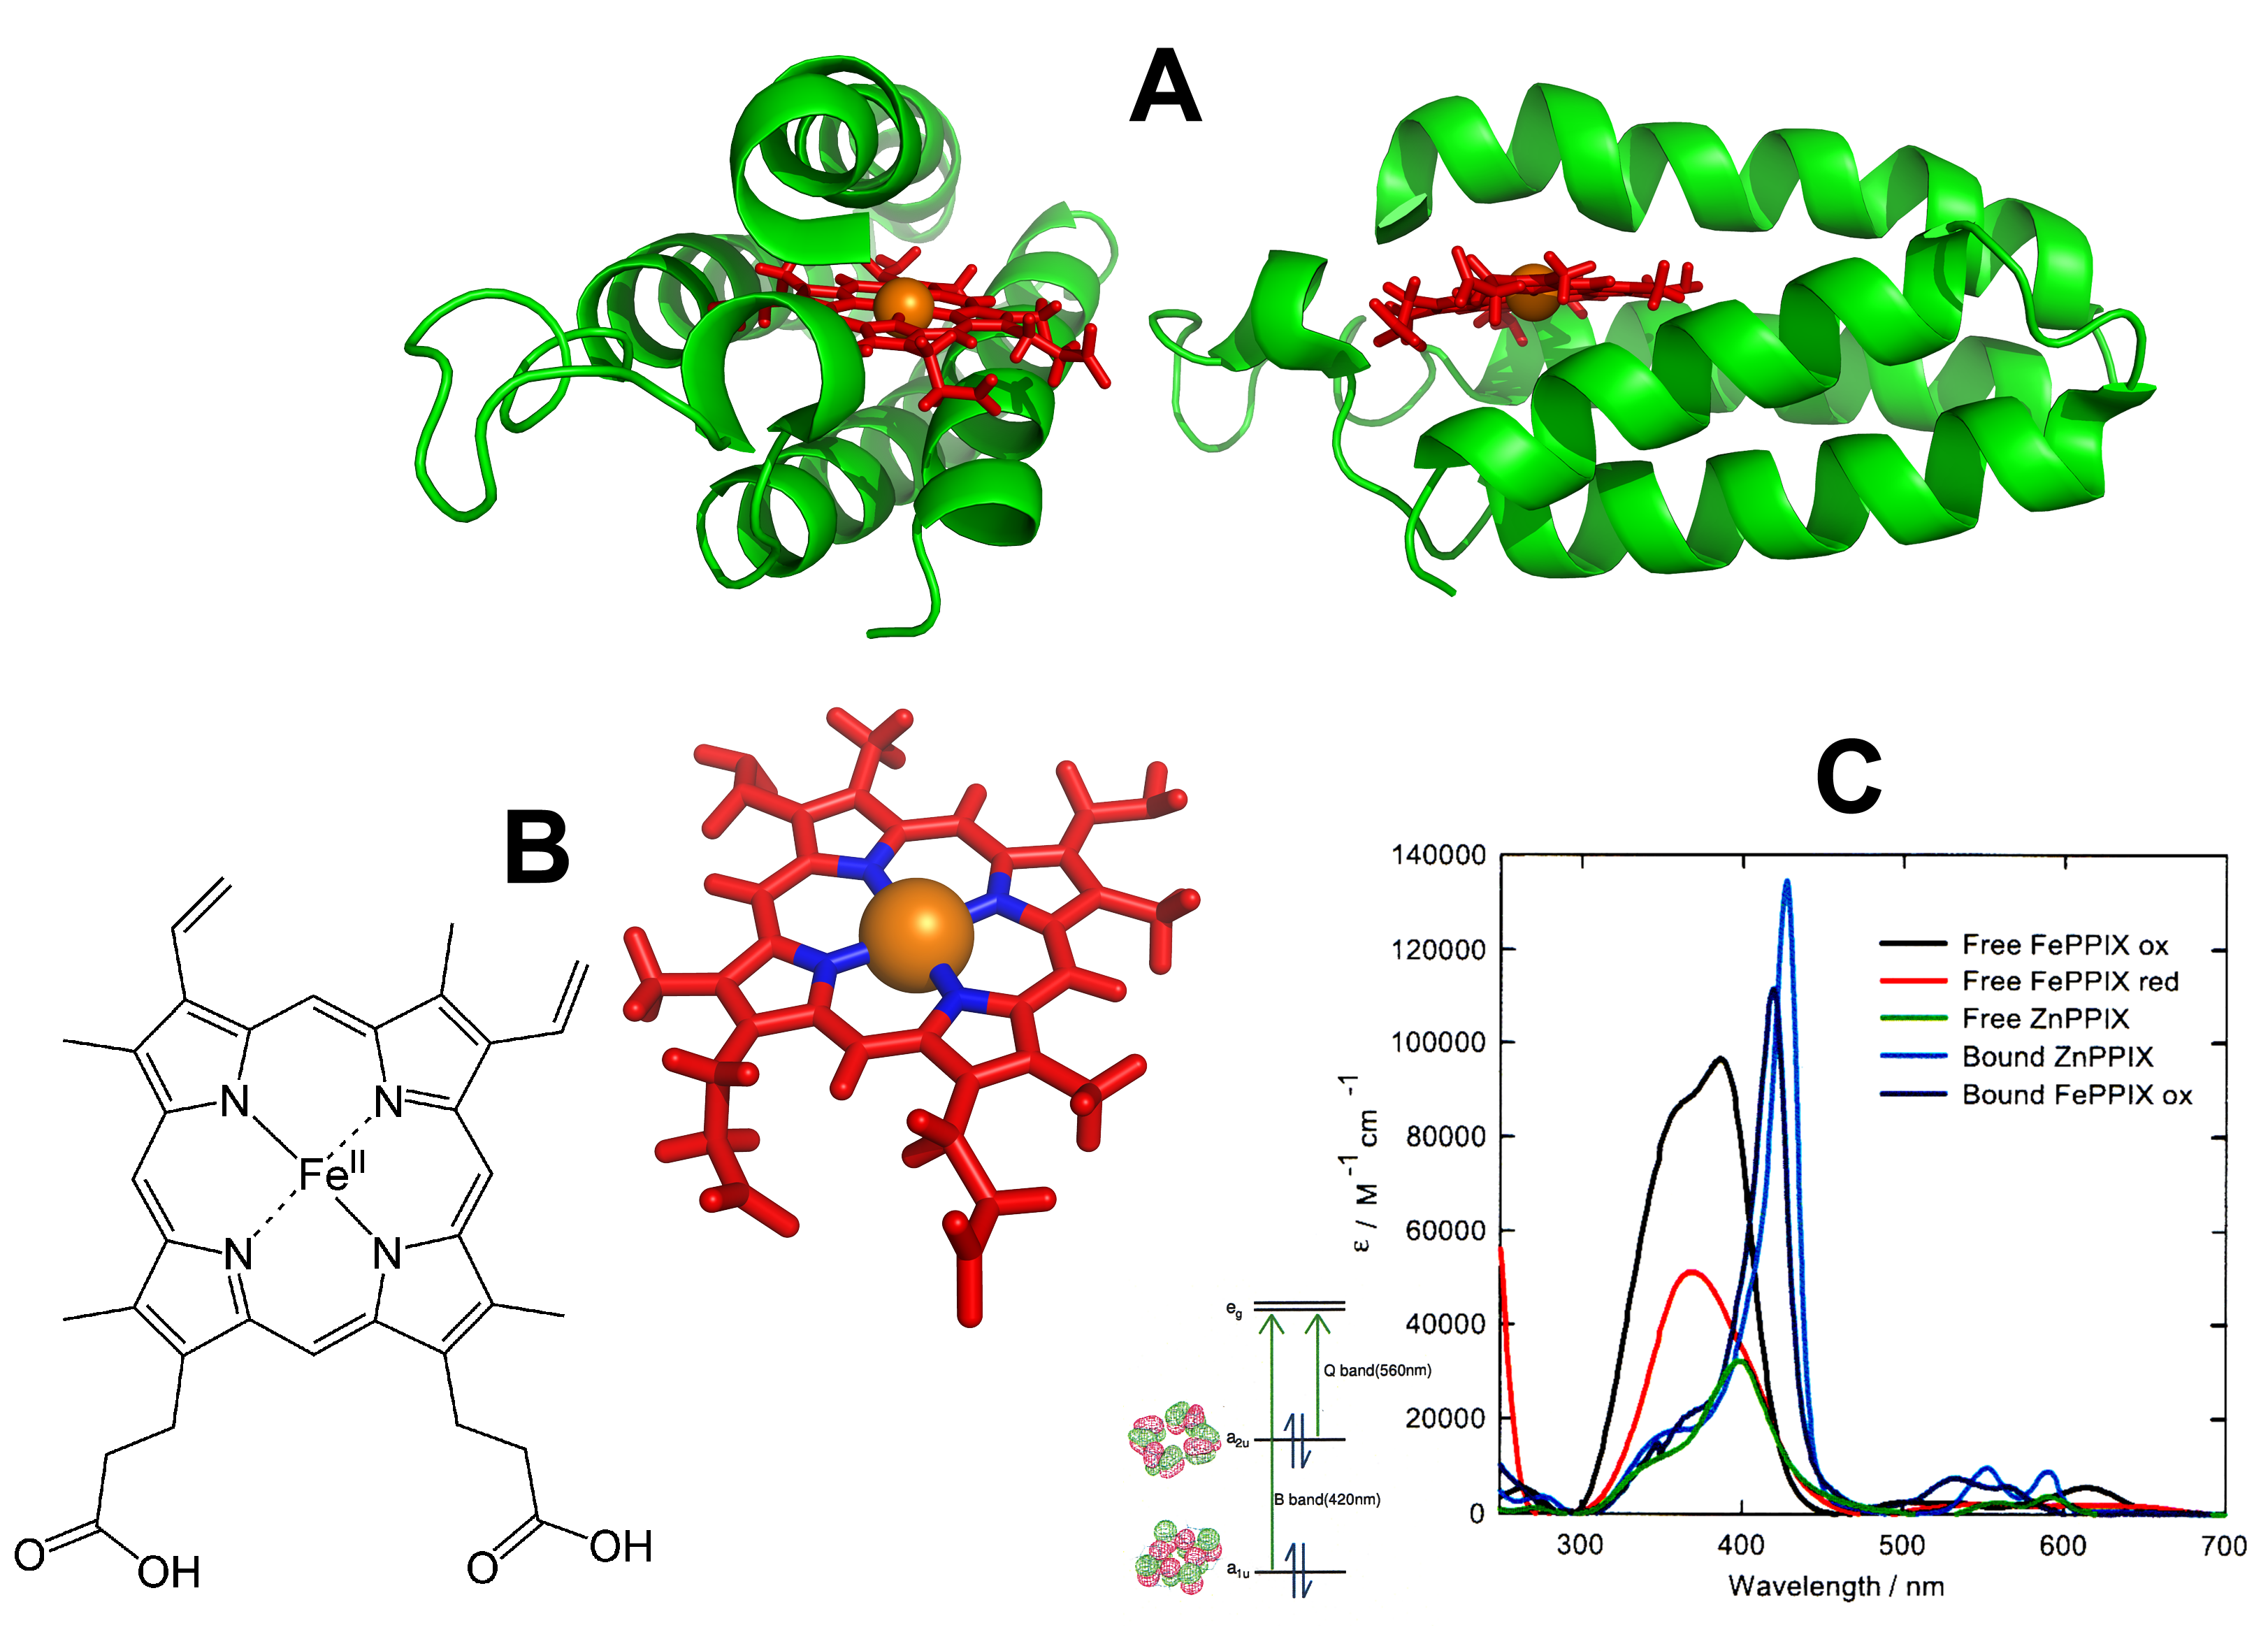
\includegraphics[width=137.4mm]{Images/haemStructure.png}
	\caption[Haem Structure]{A fancy image.}
	\label{fig:haemStructure}
\end{figure}
\end{verbatim}

\vspace{2ex}

\begin{figure}[!th]
	\centering
	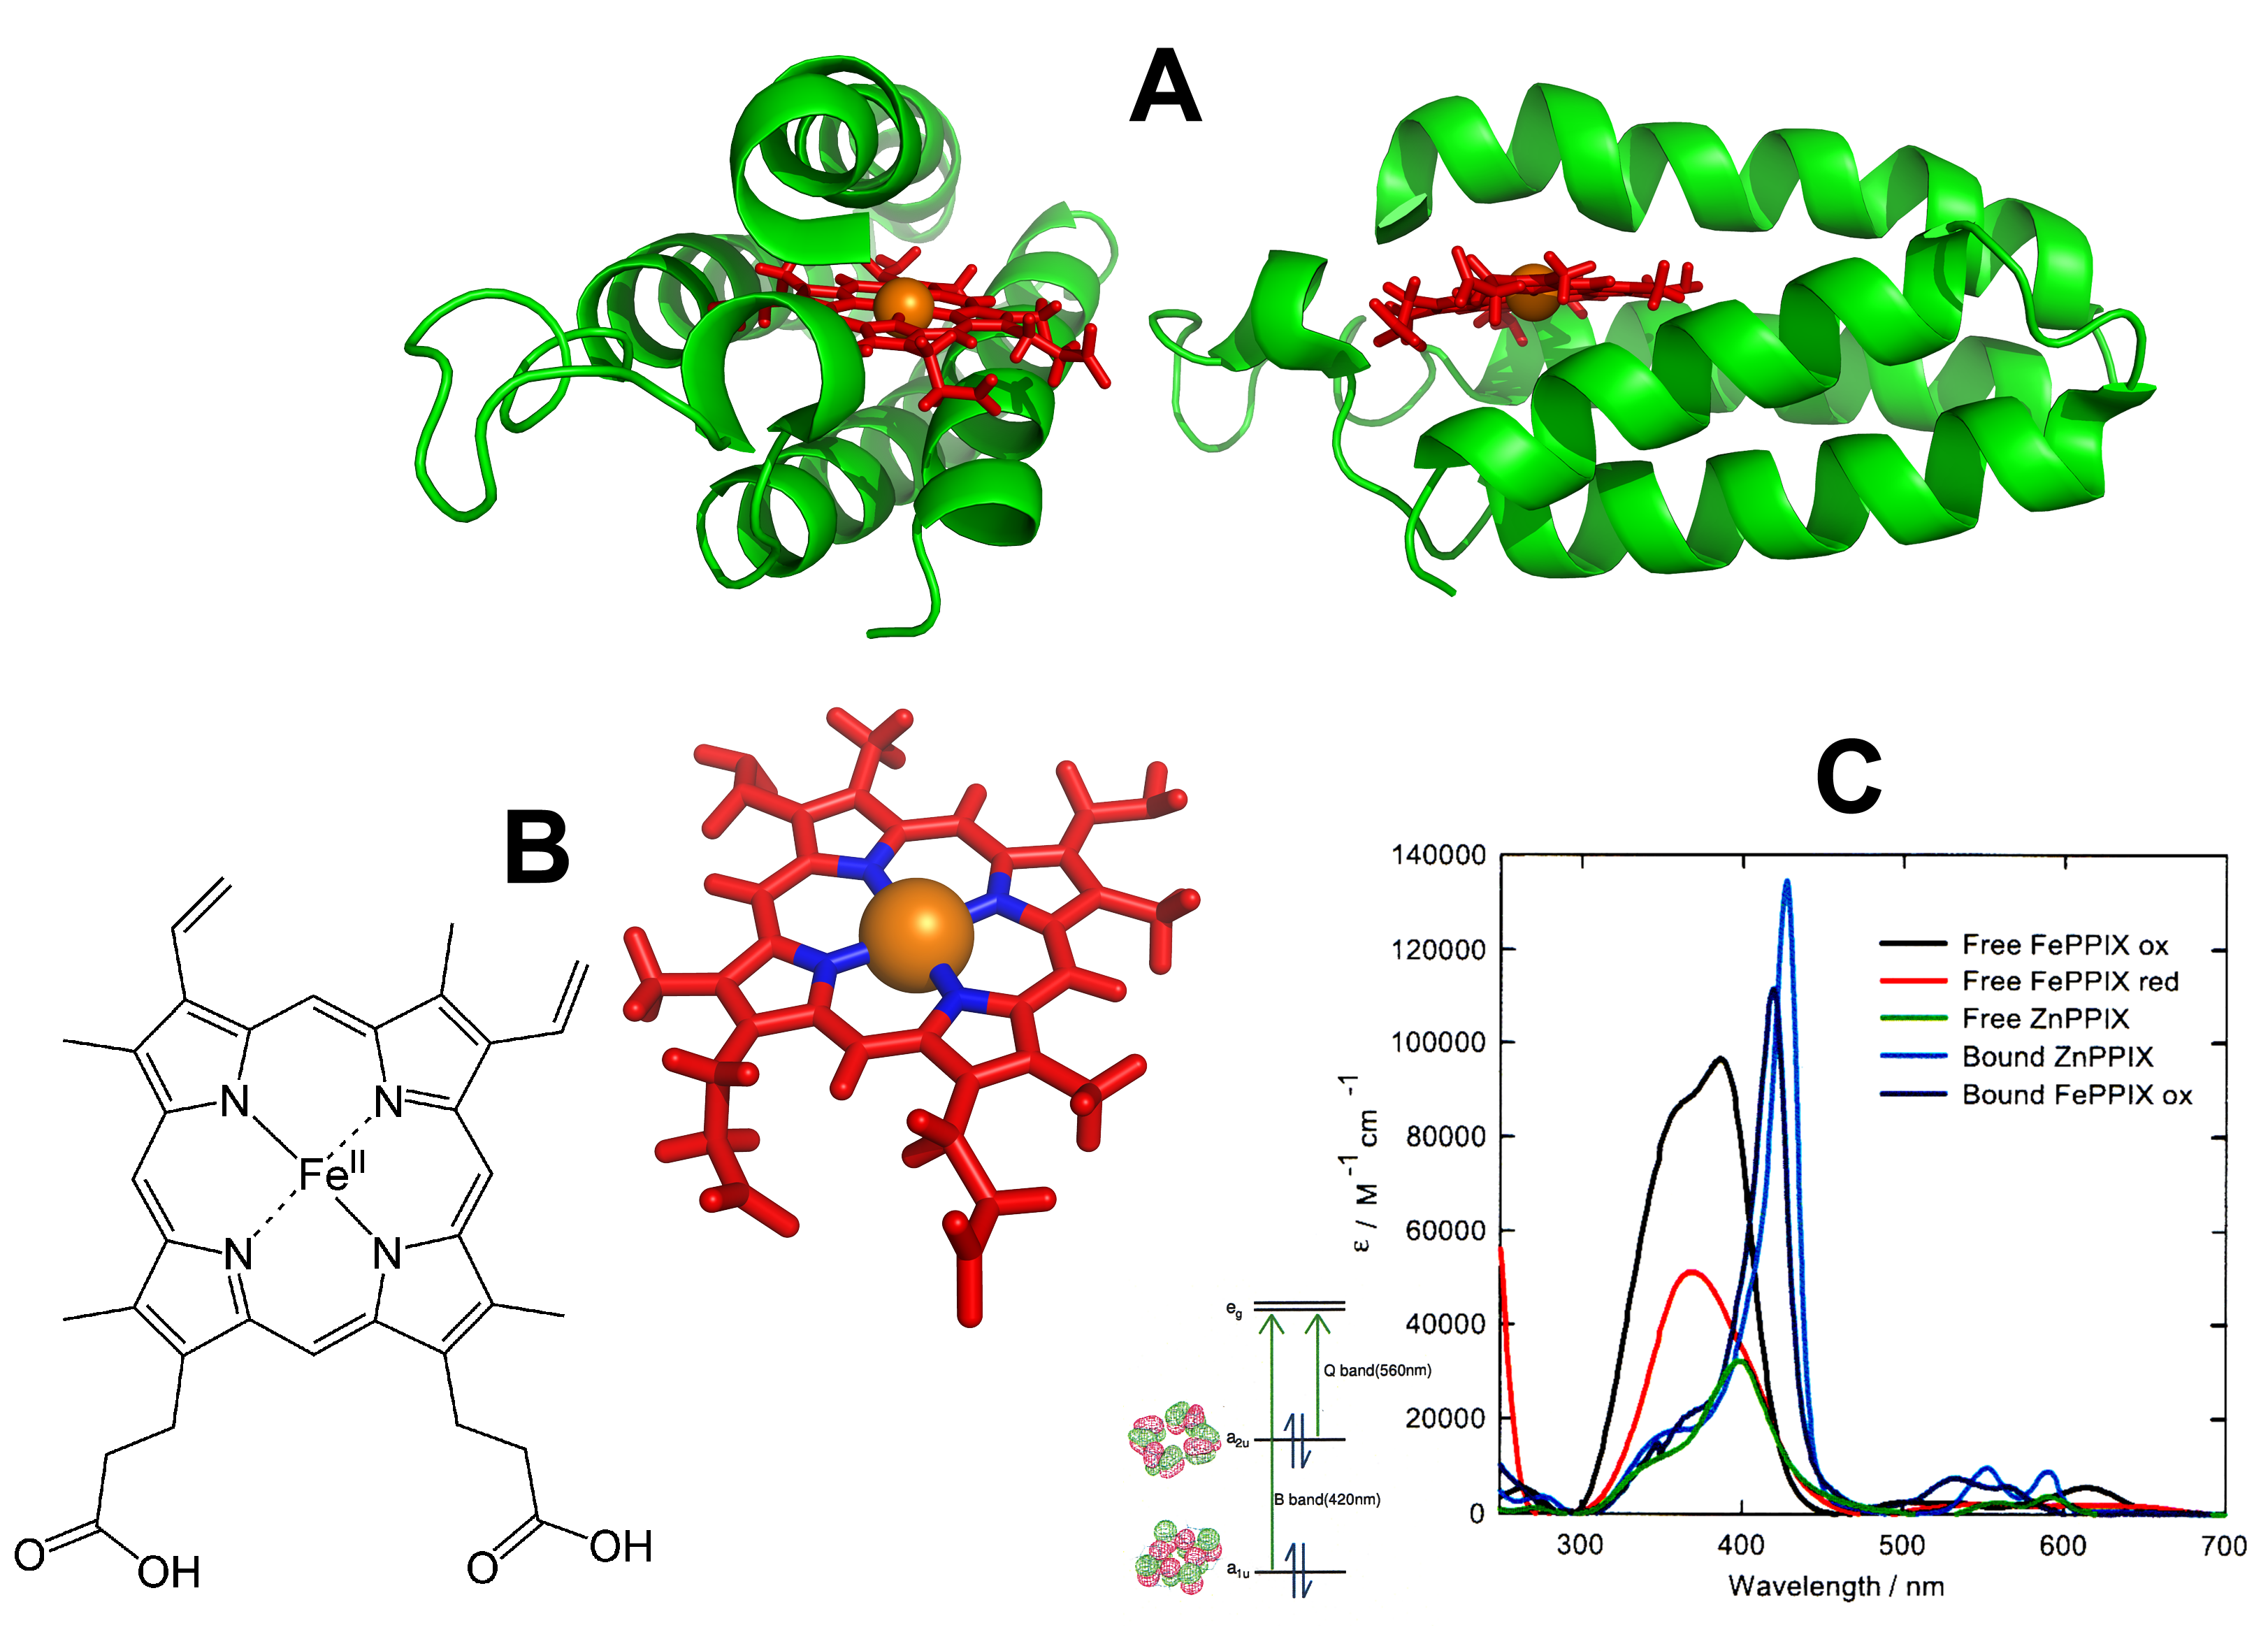
\includegraphics[width=137.4mm]{Images/haemStructure.png}
	\caption[Haem Structure]{A fancy image from Chris' Thesis.}
	\label{fig:haemStructure}
\end{figure}

In this example the command {\textbackslash}includegraphics tells LaTeX to look in the directory `Images' and incorporate the file called `haemStructure.png' into the final document while setting the width to 137.4mm.  This command can be used to resize a graphical file using the height or width parameter as shown. You must specify the units which can be pt, ex, em, mm, cm and so on. LaTeX recognises a very wide variety of standard units and graphics formats. The command is part of the graphicx package and so in the preamble you must include the command {\textbackslash}usepackage\{graphicx\}.

Many packages have been written to provide new commands. For example the `subfigure' package enables you to place separate images or files in the same figure side by side while giving them their own label. However, in this document we only concentrate on the very basics.

\section{Floating Environments}

Both tables and figures are examples of a `floating environments' which means LaTeX decides where to put them. 

The mysterious [!tbh] letters give guidance to LaTeX about roughly where the figure or table is  allowed to be, but in general they can move a long way from where you position them within your text file.  The letters in the square bracket can be t, h or b which stand for top, here or bottom.  If you don't specify any letters LaTeX defaults to [t].

LaTeX will always preserve the order in which figures appear.  If it cannot find a type setting solution, then it may move the float to it's own page, and combine it with other figures. If it still can't fit that in for some reason then it moves the float to the end of the document.  This has the effect of pushing all the remaining floating environments to the end of the document also.

The exclamation mark instructs LaTeX to ``try harder'' at putting the float where you told it to. Often you must play around to ensure the float positioning is acceptable, but usually this can be achieved by stretching or shrinking the image slightly using the size parameter, re-ordering text, judicial applications of the {\textbackslash}pagebreak command or by shouting loudly and slapping the computer monitor about. Note that it is better to resize the image using the original program that was used to create the image. Also using vector graphics can assist be useful (e.g. eps files) because they are designed to scale better.
\chapter{The Chapter on Making Chapters}
\label{sec:Chapters}

Right. LaTeX forces you to structure your document. There a series of simple commands for achieving this:

\vspace*{2ex}

{\textbackslash}chapter\{chapterName\}

{\textbackslash}section\{sectionName\}

{\textbackslash}subsection\{subsectionName\}

{\textbackslash}subsubsection\{subsubsectionName\}

\vspace*{2ex}

Easy enough. At the start of each chapter or section just issue one of these commands to name the section and LaTeX will present the chapter heading in the right style of font, which will be the same style of all the other heading names at that level of hierarchy throughout the document. In addition LaTeX assigns a number to that section. For example, this chapter was created using the command:

\vspace*{2ex}

{\textbackslash}chapter\{The Chapter on Making Chapters\} 

\vspace*{2ex}

LaTeX assigns the correct chapter number to each chapter in turn and then puts it in the table of contents, as you can see by looking at the table of contents! Easy.

\pagebreak
\section{The Section About Sections}
\label{sec:Section}
I think you're getting the hang of this. This section was created using the command {\textbackslash}section\{The Section About Sections\}. It appears in the table of contents as section \ref{sec:Section}.

\subsection{The Sub-Section About Sub-Sections}
\label{sec:SubSection}
Now you're really getting the hang of this. This subsection was created using the command {\textbackslash}subsection\{The Sub-Section About Sub-Sections\}. 

\subsubsection{The Sub-Sub-Section About Sub-Sub-Sections}
\label{sec:SubSubSection}
Now you're really getting the hang of this. but.. caught you out! This subsubsection doesn't have a number!  Ha Ha! It was created using the command {\textbackslash}subsubsection\{The Sub-Sub-Section About Sub-Sub-Sections\} in the same vein as all the other subsections/chapters etc. Here we have stopped the depth of the section numbering at the second level with the command:

\vspace*{2ex}

{\textbackslash}setcounter\{secnumdepth\}\{2\}

\vspace*{2ex}

Easy. WYSIWYM.  LaTeX does what you tell it to do. This is both a blessing and a curse.

\pagebreak
\section*{The Section About Sections That Don't Appear in the Table of Contents}
\label{sec:InvisibleSection}
Ok. Now we're throwing a spanner in the works. This section was created using the command:

\vspace*{2ex}

{\textbackslash}section*\{The Section About Sections That Don't Appear in the Table of Contents\}. 

\vspace*{2ex}

Notice how LaTeX has not assigned a number to the section and it doesn't appear in the table of contents. The effect of the * is to suppress the inclusion of a chapter, section or subsection in the automatic numbering. Easy. You can do this at any level. This is useful for things like prefaces, tables of contents or acknowledgements which you may or may not wish to have an entry in the main contents table. Up to you. It's your thesis. Don't just copy me.

\section{A Small Point About Numbering}

In this section notice how the numbering starts from where it left off before we suppressed the numbering on the previous section. Easy. WYSIWYM.
\pagebreak
\section{The Section About Internal Referencing}
\label{sec:InternalReferencing}

There are two related commands:

\vspace*{2ex}

{\textbackslash}label\{labelName\} 

{\textbackslash}ref\{labelName\}

\vspace*{2ex}


The {\textbackslash}label\{\} command allows you to create a label in a particular environment\footnote{That's right. Chapters, Sections and sub-sections etc are environments!}. The label won't appear in the final document. It's just a label which makes it easy to refer back to any particular environment elsewhere in the document. The {\textbackslash}ref\{\} command enables you to insert a reference anywhere in the document to any label in the document.  For example this is section \ref{sec:InternalReferencing}. The names you use in a label can be anything you like but musn't contain whitespace or special characters. I used the two commands:

\vspace*{2ex}

{\textbackslash}label\{sec:InternalReferencing\}

{\textbackslash}ref\{sec:InternalReferencing\}.

\vspace*{2ex}

The astute among you will realise that LaTeX has to read the document several times. Once to find the labels and then again to populate the references with the correct numbers. So you have to compile a latex document twice to get the referencing right. If there is a missing label or you refer to something that doesn't exist then latex inserts a convenient ? at that point. So hunting for queries is useful way of finding broken references. Latex issues warnings when it finds broken references.

As you create a document you will find yourself putting labels in all over the place so choose a sensible naming convention to help you remember the label names.

Each type of environment (equations, figures, tables, sections etc) has its own independent numbering system.  So when you choose your label name it's a good idea to have an identifier for that type of environment.  I have my own convention for label names which I use to help me remember references. E.g.   sec:SectionAboutCats. Eqn:EquationAboutCats,  Fig:FigureAboutCats and so on. This means you can differentiate between referring to the section or the figure more easily, even though they are about the same thing.

So Internal Referencing is a doddle. Easy!
\chapter{External Referencing}

Referencing is usually performed using a separate program called BibTex.  This program understands the file format .bib.

To create a reference within your document first you must create a .bib file by exporting your list of references from which ever referencing software you used, such as endnote, mendeley or whatever you use.

You can refer to an entry in the .bib file using the {\textbackslash}cite\{ref:Name\} command. the identifier `ref:Name' is the unique identifier which is the first line of each item included in your bibliography file.

For example, open the file LaTexCourseBib.bib in the bibliography directory. The first entry has the identifier `Horcas2007'.  This can be invoked as follows:


\begin{verbatim}
For example, this interesting fact\cite{Horcas2007}, is a cracking example.
\end{verbatim}

For example, this interesting fact\cite{Horcas2007}, is a cracking example.

During compilation latex and bibtex co-operate. During the first compilation latex generates a list of references that it needs.  During the second compilation bibtex populates the details from the .bib file into a shorter, ordered .bib file. The third compilation inserts markers at the right place in the main file and the fourth compilation generates the final list of references. Thus the compilation sequence is latex, bibtex, latex, latex.

The style of the referencing format can be changed using the command {\textbackslash}bibliographyStyle\{\}. e.g. the style used in this document is cjfthesisv1.bst which is invoked by 

\begin{verbatim}
\bibliographystyle{Bibliography/cjfthesisv1}
\end{verbatim}

The location of the list of references in the document is specified by issuing the {\textbackslash}bibliography\{\} command which also specifies the master bibliography file.

\begin{verbatim}
\bibliography{Bibliography/LaTeXCourseBib}
\end{verbatim}




\chapter{Organising Your Files}
One of the drawbacks of word is that the figures and tables are included within the document which becomes very very clunky quite quickly and once it reaches around 100Mb it becomes unwieldy and hard to export. One of that advantages of LaTeX is that the files are all text files and so are very light on resources and are easy to email around the place.

However, sometimes it can be difficult to navigate through a single text file, so if you had a huge document then it becomes difficult to find your way around.  One way of circumnavigating this problem is to break the file up into smaller files. As long as LaTeX knows where to look you can have a file for each logical sub-division of your document.

Therefore it is worth spending a bit of time at the beginning of a large project deciding how you wish to break up your LaTex Files and organise them neatly and tidily.  You can then tell LaTex where to look for the files using the following command:

\vspace*{2ex}
{\textbackslash}include\{fileName\}
\vspace*{2ex}

\pagebreak
\section{Linking a File}
We are now going to copy part of the tutorial file into a separate files and link it the main file.  Because this could go wrong it is sensible to back up tutorial.tex as something else. So save a copy called `tutorialOriginal.tex' for safe keeping. Then follow the following instructions.

\begin{enumerate}
\item Create a new file called MyFirstPage.tex
\item Select and Cut out the first chapter of Tutorial.Tex
\item Paste the first chapter into MyFirstPage.tex
\item Save both tutorial.tex and MyFirstPage.tex
\item Then add {\textbackslash}include\{MyFirstPage\} in tutorial.tex where the text used to be before you cut it out. We don't need to add the `.tex' because LaTeX can only include `.tex' files.
\item compile tutorial.tex and view the PDF
\end{enumerate}

The final PDF should look exactly the same as it was! except we now have a separate file for one of the chapters.

\pagebreak
\section{Creating A Class File}
We can also save our preamble in a separate file called a class file. This makes your main document much easier to understand.  To make it work we need to use the {\textbackslash}LoadClass\{\} command as follows: 

\begin{enumerate}
\item Create another new file and save it as TutorialStyle.cls
\item Copy the preamble of tutorial.tex into the new file. Starting with the {\textbackslash}documentclass{} command and copy right up to, but not including, the {\textbackslash}begin{document} command. Delete the preamble in the original document.
\item Save TutorialStyle.cls and tutorial.tex
\item Modify the first line of TutorialStyle.cls by replacing the word `document' with the word `Load'.
\item Add a new first line of tutorial.tex to use your new style class {\textbackslash}documentclass\{TutorialStyle\}
\item Save both files.
\end{enumerate}

\subsection{Sanity Check}

The first line of TutorialStyle.cls should now be:

\begin{verbatim}
\LoadClass[12pt, oneside, a4paper]{book}
\end{verbatim}
\vspace{2ex}

The first line of tutorial.tex should be:

\begin{verbatim}
\documentClass{TutorialStyle}
\end{verbatim}
\vspace{2ex}

We have just created what is called a style file. You can use this style file as a generic preamble for other documents as well. Compile tutorial.tex.  Nothing should have changed in the final PDF.


\pagebreak
\section{The Structure of this Document}

Lets now look at how I've organised this document. It is identical to my thesis because it started out life as my thesis. I usurped the structure and simply replaced the headings and content to make a kind of reference manual for this introductory course. This document therefore is three things:

\begin{enumerate}
\item An example thesis structure to work from.
\item The LaTeX files which were used to create it can be used as a template for a thesis.
\item It is also a convenient introductory latex manual!
\end{enumerate}

\vspace*{2ex}
Groovy huh?

\section{The Master File}

There is a master file where LaTeX begins the compilation procedure. This contains the {\textbackslash}documentclass command needed to set the ball rolling. Within the file there are a series of {\textbackslash}include\{\} commands, one for each Chapter, which tell LaTeX where to find the files containing each chapter.

The subfiles cannot be compiled on their own because they do not contain the {\textbackslash}documentclass, {\textbackslash}begin\{document\} or {\textbackslash}end\{document\} commands. Lets us look in more detail at the master file and we will learn some new LaTeX commands.

\singlespacing
\pagebreak
\begin{verbatim}
\documentclass{Style/LatexCourseStyle}

\begin{document}
\setcounter{secnumdepth}{2}
\setcounter{tocdepth}{1}

\frontmatter
\onehalfspacing
\thispagestyle{empty}

\begin{center}
\vspace*{\stretch{1}}

\hrule height 2pt
\vspace*{2ex}
{\Huge\textbf{Towards the Ability to Make Super Duper LaTeX Documents}\par}
\vspace*{2ex}
\hrule height 2pt
\vspace*{10ex}
{
\includegraphics[height=40mm]{Images/UnivShield}\par}
\vspace*{10ex}
{\large\textbf{Christopher~James~Forman}\par}
\vspace*{2ex}
{\large{Department Of Chemistry}\par}
\vspace*{2ex}
{\large{University of Cambridge}\par}
\vspace*{5ex}
{\large{This dissertation is submitted for the degree of \textit{Doctor of Philosophy}}\par}
\vspace*{5ex}
{\large{\today}\par}

\vspace*{\stretch{2}}
\end{center}
\chapter*{Declaration}

\vfill

This dissertation is the result of my own work and includes nothing which is the outcome of work done in collaboration except where specifically indicated in the text. It is not substantially the same as any that I have submitted for a degree or diploma or other qualification at any other University and no part has already been, or is concurrently being, submitted for any degree, diploma, or other qualification. It does not exceed 60,000 words, including tables, footnotes, bibliography and appendices.\par

\vspace{10ex}

\begin{flushright}
Signature: \rule[0pt]{60mm}{0.5pt}

\vspace{5ex}

Date: \rule[0pt]{60mm}{0.5pt}
\end{flushright}

\vfill
\chapter*{Acknowledgments}
\subsection*{Family}
Mum. Dad. Pet Dog.

\subsection*{Scientific Collaborations}
Dr A.N.Other at uni of blah for samples and instrument time etc. My Amazing Lab Chums.

\subsection*{Scientific Support}
My amazing lab chums.

\subsection*{General Assistance}
Cleaner, My amazing lab chums.

\subsection*{Financial Support}
Bank, Tax payer. My amazing lab chums.

\subsection*{Moral Support}
My Amazing Lab chums.

\subsection*{Academic Inspiration}
Netwon, My super. My Amazing Lab Chums.

\subsection*{Everyone else}
My Amazing Lab Chums.

\chapter*{Summary}
This document is a handbook for introducing you to LaTeX. It contains a bit of background about the history and philosophy of LaTeX.  However, it concentrates on providing a guided practical introduction to the basic techniques such as 
\begin{itemize}
\item Lists
\item Mathematical and chemical equations
\item Tables
\item Figures
\item Chapters and Sections
\item Linking to other files in large documents
\item Referencing
\end{itemize}

The handbook is also presented in the style of a thesis. This means that source files provided on the introductory course and available from the department web page are a convenient template for a thesis.

More details on specific aspects of LaTeX can be found at the departmental LaTeX page which can be found here:

 http://www-ch-int.ch.private.cam.ac.uk/latex/about

\chapter*{Abbreviations}

\begin{longtable}{r >{\rule{0pt}{3ex}}l<{\rule[-1.5ex]{0pt}{0pt}}}
ADP & Adenosine Diphosphate\\
(nc/c)AFM & (non-contact/conducting) Atomic Force Microscopy\\
ATP & Adenosine Triphosphate \\
\end{longtable}
\tableofcontents
\listoftables
\listoffigures

\mainmatter
\renewcommand{\sectionmark}[1]{\markright{\thesection \ #1}{}}
\chapter{Overview}
\label{chap:overview}
\section{LaTeX: The answer to everything.}
LaTeX is typsetting program that takes an input file of marked up text and then, with a user defined set of rules, typesets a beautifully crafted output file that can be easily printed (e.g. a pdf). 

\subsection{Advantages}

The advantages of this method are manifold:

\begin{itemize}

\item Use any text editor to view the source document.
\item More time can be spent working on the content and not worrying about how text or figures interact in the layout until later on.
\item LaTeX uses consistent rules throughout a document
\item LaTeX sorts out basic typesetting automatically
\item Changes can be introduced globally with very little effort
\item Document structure is explicit
\item Documents can be professionally typeset and look great
\item You are forced to structure your documents correctly.
\item Mathematical equations, like $E=mc^2$ or $\imath\hbar\frac{\partial}{\partial t}\Phi (x, t) = \hat{H}\Phi (x, t)$ can be produced almost as fast as typing (if you know the commands!).
\end{itemize}

\subsection{Disadvantages}
The disadvanatges of this method are also manifold:
\begin{itemize}
\item You don't see the output as you go.
\item Steep learning curve.
\item Documents are harder to edit by a second author (unless they are adept at LaTeX too). This can be mitigated using version control, which makes group authoring processes superior to word.
\item The program never works quite the way you want it to and learning how to influence it can be problematic and subtle.
\item Although intended to save work the principle of 'conservation of work' means that you simply transform problems associated with WYSISYG approaches to problems associated with WYSIWYM approaches!
\item You can go blind trying to determine the difference between wiggly and smooth brackets if your editors font isn't large enough.
\end{itemize}

\subsection{On balance?}
If it's so rubbish, why use LaTeX?

\begin{itemize}
\item Large documents are much more easily handled. 
\item In general it is quicker to debug a LaTeX document than typeset an entire thesis manually. 
\item Technical information such as tables, equations and figures are integrated much more smoothly than with word.
\end{itemize}

\section{How does it work?}

The raw text is interspersed with commands, preceded by a \textbackslash, which tell LaTeX what to do with the text. For example you can \textbf{make it bold}, \emph{italic}, or \underline{underlined} with the commands {\textbackslash}textbf\{\}, {\textbackslash}emph\{\} or {\textbackslash}underlined\{\}. More on commands in a moment...



\chapter{My First Page}

\section{The Very Beginning}
The very simplest LaTeX document might look like this:

\begin{verbatim}
\documentclass[a4paper,12pt]{article}
\begin{document}
Hello World.
\end{document}
\end{verbatim}

\pagebreak
\thispagestyle{empty}
Hello World.
\pagebreak
\subsection{Break Down}
What's all the gobbledegook around my simple message???

In LaTeX we intersperse text and commands.  Commands are preceded by a \textbackslash. For example the first line in a LaTeX document \underline{\textbf{\emph{must}}} be:

\begin{verbatim}
\documentclass[options]{class}
\end{verbatim}

Where the word ''class'' may be substituted for one of many things such as: article, proc, minimal, report, book, letter, memoir, slides, beamer.

Similarly, and completely generally in LaTeX speak, the square brackets denote the existence of optional parameters. Each individual command can take its own parameters and for the ''{\textbackslash}documentclass'' command there are options for controlling font size, font family, landscape, oneside, twosided, page size and so on. These options will persist throughout the entire document. For example the document class command for this document, (which is likely to be like the one you would use for a thesis), would be:

\begin{verbatim}
\documentclass[12pt, oneside, a4paper]{book}
\end{verbatim}

Other options include:

\begin{itemize}
\item {10pt, 11pt, 12pt (default is 10pt).}
\item {letterpaper, legalpaper, a4paper, executivepaper, a5paper, b5paper}
\end{itemize}
and so on.

\pagebreak
\section{Can I start typing please?}

After we have set up the document we can start actual work on our document. So we must tell LaTeX that what follows is to be interpreted as a document.  The command {\textbackslash}begin can take many different parameters and is a command to enter what is known, in LaTeX speak, as 'an environment'. Thus the commands:
\begin{verbatim}
\begin{document}

\end{document}
\end{verbatim}

tells LaTeX to enter and leave the document environment, and thus constitute the outer limits of our document file. Other environments include the equation environment, the itemize environment, the figure environment and so on. These will be encountered in due course.

Every part of the LaTeX file is therefore within an environment of specific type and the content within each environment consists of commands or text.

That's basically it.

So let's get on with it shall we...

\pagebreak
\section{The ground rules}
\begin{quote}
Hold on, hold on, hold on my son.

First the lessons.

Then the fun!
\end{quote}
Dr Seuss.

\subsection{Spaces}
Whitespace characters, such as blank or tab, are treated uniformly as space by LaTeX. Several consecutive whitespace characters are treated as one single space. Whitespace at the start of a line is generally ignored, and a single line break is treated as whitespace. An empty line between two lines of text defines the end of a paragraph. Several empty lines are treated the same as one empty line. The text below is an example.

\begin{verbatim}
It does not matter whether you
enter one or several             spaces
after a word. The final result will be typeset beautifully
according    to     precise rules.




An empty line starts a new
paragraph. Note the indentation on the first line of the paragraph, 
except at the beginning of the section. 
\end{verbatim}

\vspace*{2ex}
\vspace*{2ex}

It does not matter whether you
enter one or several             spaces
after a word. The final result will be typeset beautifully
according    to     specific rules.




An empty line starts a new
paragraph. Note the indentation on the first line of the paragraph, except at the beginning of the section. 

\pagebreak
\subsection{Special Characters}
The symbols 

\# \$ \% \textasciicircum{} \& \_ \{ \} \~{} \textbackslash

are reserved characters that either have a special meaning under LaTeX or are unavailable in all the fonts. If you enter them directly in your text, they will normally not print, but rather make LaTeX do strange things.

To overide the special meanings of these symbols and allow them to produced within your text you may use the following sequences:
\begin{verbatim}
\# \$ \% \textasciicircum{} \& \_ \{ \} \~{} \textbackslash
\end{verbatim}

Other symbols and many more can be printed with special commands in mathematical formulae or as accents.

The backslash character '\textbackslash' cannot be entered by adding another backslash in front of it ( \textbackslash\textbackslash); because this sequence means ''linebreak''.

The command \textbackslash\~{}\{\} produces a tilde which is placed over the next letter. For example \textbackslash\~{}\{n\} gives \~{n}. To produce just the character \~{}, use \textbackslash\~{}\{\} which places a \~{} over an empty box.

Similarly, the command \textbackslash\textasciicircum{} produces a hat over the next character, for example \textbackslash\textasciicircum\{o\} produces \^{o}.

\pagebreak
\section{Preamble}
After the {\textbackslash}documentclass command we add ''preamble''. Here we load special features that we will use throughout our document to expand on the basic capabilities of LaTex. These are contained in units called ''packages'' which we can tell our LaTeX compiler to download by using the command ''{\textbackslash}include\{packageName\}''. 

There are many repositories of such packages on the web. Your compiler generally knows where to look and most standard packages are included with any install. For example, to include a special set of typesetting instructions to handle chemical equations we can grow our simple document with a single command like this:

\begin{verbatim}
\documentclass[a4paper,12pt]{article}
\usepackage[version=3]{mhchem}
\begin{document}
Hello World!

We all need \ce{H2O}.

I'm less fussed about \ce{^{235}_{92}U+}.

\end{document}
\end{verbatim}

\vspace{2ex}

\pagebreak
\thispagestyle{empty}
Hello World!

We all need \ce{H2O}.

I'm less fussed about \ce{^{235}_{92}U+}.
\pagebreak

Here we have loaded a package called: "`mhchem"' which took the option ''[version=3]''. This is a package for drawing chemical equations easily and it has it's own instruction manual which you can follow easily. It is included in the bundle of files for this course.

Other things we can do in the premable within LaTeX are to redefine existing commands or create our own personal commands. These can be stored in a file called the 'style file' which we can load at the beginning of our document, in place of our documentclass. More about this later on...


\subsection{Comments}
It is often useful to comment your LaTeX documents. You can leave yourself amusing, sarcastic messages that won't get printed out in the final document. Use this to make your own notes as the course progresses.

To get a comment use the \% command, which tells LaTeX to ignore the rest of the line, the line break and all the white space at the beginning of the next line, for example, we may add to our continually evolving document...

\begin{verbatim}
\documentclass[a4paper,12pt]{article}
\usepackage[version=3]{mhchem}
\begin{document}
Hello World!

%All humans need water and I would like 
%to include this concept in my arguments.
We all need \ce{H2O}.

%Uranium 235 is toxic, which is why I don't want to consume it... 
I'm less fussed about \ce{^{235}_{92}U+}.

\end{document}
\end{verbatim}

\vspace{4ex}
Hello World!

%All humans need water and I would like to include this concept in my arguments.
We all need \ce{H2O}.

%Uranium 235 is toxic, which is why I don't want to consume it... 
I'm less fussed about \ce{^{235}_{92}U+}.

\pagebreak
\section{Compiling}
Once the document is finished you can compile it. Your compiler will depend on the platform that you use. In the PWF we are using winEDT to edit the documents (a LaTeX front end) and texlive2008 which is the compiler itself. I use MiKTex and the front end texCenter.  There is no need to use a front end. If you prefer you can use a simple text editor and a command line.

the recommended distributions are:
\begin{itemize}
\item MiKTeX or TeX Live for Windows
\item TeX Live for Unix/Linux
\item MacTeX or TeX Live for Mac OS.
\end{itemize}

Once you have installed your software and got it working, written your source code and tried to compile it, there will nearly always be something wrong with your file. 

Any errors will be highlighted in the console window or error output box of your front end.  Some front ends dump the running commentary which LaTeX produces into a text file for easy reading afterwards.

In a compile attempt (successful or otherwise) LaTeX may produce the following files:

projectname.aux

projectname.bbl

projectname.lof

projectname.lot

projectname.txt

projectname.toc

projectname.dvi

These are interim files (toc= table of contents, bbl = bibliography etc). To be honest I have no idea what half of these things contain.  You only need the .tex file and a compiler with the right packages installed to produce them again.

Some versions of LaTeX only produce DVI files and you then need to convert the dvi file to a PDF or download a dvi viewer. You can also convert DVI files to PS files and then view them.  The good thing about front ends is that you can set them up to produce PDFs directly.

OK. So we have now produced a silly document but we understand it.  Now lets get on with learning how to make our own documents.



\chapter{Lists}
Lists are great.  The command {\textbackslash}begin\{\} can be used to enter a list environment.  For example:

\begin{verbatim}
\begin{itemize}
\item cat
\item dog
\item horse
\end{itemize}
\end{verbatim}

Produces:

\begin{itemize}
\item cat
\item dog
\item horse
\end{itemize}

\pagebreak
We can also replace the bullet points with numbers using the enumerate keyword.

\begin{verbatim}
\begin{enumerate}
\item cat
\item dog
\item horse
\end{enumerate}
\end{verbatim}

\begin{enumerate}
\item cat
\item dog
\item horse
\end{enumerate}

\pagebreak
and we can use the description keyword which does this:
\begin{verbatim}
\begin{description}
\item[Cat] a lovely furry creature with a cute nose and whiskers.
\item[Dog] Another furry creature that smells rather well; 
           its olfactory power stems from its nasal dampness.
\item [Horse] A large stinky creature with sideways facing eyes.
\end{description}
\end{verbatim}

\begin{description}
\item[Cat] a lovely furry creature with a cute nose and whiskers.
\item[Dog] Another furry creature that smells rather well; its olfactory power stems from its nasal dampness.
\item [Horse] A large stinky creature with sideways facing eyes.
\end{description}
\chapter{Maths Equations}

\section{Producing Beautiful Looking Mathematics}

One of the best features about LaTeX is `maths mode'.  For example the schrodinger equation can be produced as follows:

\vspace*{2ex}

\begin{center}
\begin{math}
\imath\hbar\frac{\partial}{\partial t}\Phi (x, t) = \hat{H}\Phi (x, t)
\end{math}
\end{center}

\vspace*{2ex}

\begin{verbatim}
\begin{math}
\imath\hbar\frac{\partial}{\partial t}\Phi(x,t)=\hat{H}\Phi(x,t)
\end{math}
\end{verbatim}

There are a number of ways to switch on maths mode.  The first, as above, is with the {\textbackslash}begin\{math\} environment. You can also enter mathmode inline using the \$ symbol. For example typing in \$y=ax\textasciicircum{}2+bx+c\$ yields $y=ax^2+bx+c$.  Another way is to enter the equation environment which enables you to number equations so you can then refer to them later in the text.

\begin{equation}
y(t)= \sin \left(\frac{{\alpha}t}{2\pi} + \phi_0\right)
\label{eqn:MadeUpNonsense}
\end{equation}

\vspace*{2ex}
\begin{verbatim}
\begin{equation}
y(t)= \sin \left(\frac{{\alpha}t}{2\pi} + \phi_0\right)
\end{equation}
\end{verbatim}.

\section{Basic Maths Mode}
Once in maths mode there is a kind of text based code for writing down your equations.  Here are the most basic symbols to get you going.
\begin{center}
\begin{tabular}{cc}
\toprule
Final Result & LaTeX Code \\
\cmidrule(){1-2}
$a+b$ & a+b \\
$a-b$ & a-b \\
$ab$ & ab \\
$a*b$ & a*b \\
$a \times b$ & a {\textbackslash}times b \\
$a \cdot b$ & a {\textbackslash}cdot b \\
$\frac{a}{b}$ & {\textbackslash}frac\{a\}\{b\} \\ 
$a^b$ & a\textasciicircum{}b \\
$a_b$ & a\_b \\
$\sin a$ & {\textbackslash}sin a  (same for cos, tan)\\
$ sin a$ & sin a \\
$\sqrt{a}$ & {\textbackslash}sqrt\{a\} \\
$\left( a \right) $ & {\textbackslash}left( a {\textbackslash}right)\\ 
$\left[ a \right]$ & {\textbackslash}left[ a {\textbackslash}right]\\ 
$\alpha$ & {\textbackslash}alpha \\
$\pi$ & {\textbackslash}pi \\
\bottomrule
\end{tabular}
\end{center}

A full treatise on maths mode is not practical here. There are lots of online tutorials and summaries of symbols. It just takes a bit of practice and you can build up equations really easily. It's straight forward to learn new stuff once you've done it a few times.

\pagebreak
\section{Equation Arrays}
Sometimes you need to arrange several equations vertically, referencing individual lines separately and aligning the equations on the $=$ sign. This can be achieved with equation arrays as follows:

\begin{eqnarray}
A\left( x\right) & = & \frac{x^2+2x+1}{x+1} \\
& = & \frac{\left(x+1\right)\left(x+1\right)}{x+1} \nonumber\\
& = & x+1 \nonumber\\
B(x,t) & = & \frac{e^{\left(\imath\omega_0 t + kx\right)}}{4\pi\epsilon_0}
\end{eqnarray}

\begin{verbatim}
\begin{eqnarray}
A\left( x\right) & = & \frac{x^2+2x+1}{1+x} \\
& = & \frac{\left(x+1\right)\left(x+1\right)}{1+x} \nonumber\\
& = & x+1 \nonumber\\
B(x,t) & = & \frac{e^{\left(\imath\omega_0 t + kx\right)}}{4\pi\epsilon_0}
\end{eqnarray}
\end{verbatim}

\begin{itemize}
\item Note the \& symbols. This tells LaTeX where to align the equations. There must be the same number of \& symbols in each line.
\item Note the \textbackslash\textbackslash ~at the end of each line except the last one. This symbol tells LaTeX to add another row in the array.  If you put it on the last line you get an empty row at the bottom of the array.
\item Note the {\textbackslash}nonumber command which suppresses line numbering for that line.
\item Note that equation number carries on from equation \ref{eqn:MadeUpNonsense} in the previous section.
\end{itemize}

\section{Maths Packages}

Maths mode comes as standard in LaTeX, however you can download packages that buff up your maths symbol set. For example neat vector notation comes in the package `vector'. e.g. {\textbackslash}uuvec\{T\} yields $\uuvec{T}$.

\begin{verbatim}
\usepackage{amssymb}
\usepackage{amsmath}
\usepackage{vector}
\end{verbatim}


\chapter{Chemical Equations}
The mhchem package means you can do basic stuff very easily using {\textbackslash}ce\{\}. For example:

\vspace{2ex}
\begin{verbatim}
\ce{CO2 + C -> 2CO}
\ce{CO2 + C <- 2CO}
\ce{CO2 + C <=> 2CO}
\ce{A-B=C#D\sbond E\dbond F\tbond G}
\end{verbatim}
\vspace{2ex}
\begin{center}
\ce{CO2 + C -> 2CO}

\ce{CO2 + C <- 2CO}

\ce{CO2 + C <=> 2CO}

\ce{A-B=C#D\sbond E\dbond F\tbond G}
\end{center}

\vspace{2ex}
You can also use math mode within chemical equations.
\vspace{2ex}

\begin{center}
\ce{$x\,$ Na(NH4)HPO4 ->[\Delta] (NaPO3)_{$x$} + $x\,$ NH3 ^ + $x\,$ H2O}
\end{center}

\begin{verbatim}
\ce{$x\,$ Na(NH4)HPO4 ->[\Delta](NaPO3)_{$x$} + $x\,$ NH3 ^ + $x\,$ H2O}
\end{verbatim}

And you can number chemical reactions as well by using the math mode equation environment.

\begin{equation}
\ce{CO2 + C <=> 2CO}
\end{equation}

\begin{verbatim}
\begin{equation}
\ce{CO2 + C <=> 2CO}
\end{equation}
\end{verbatim}

However, this will number mathematical and chemical equations using the same number system. There is a discussion in the mhchem pdf which shows you how to number chemical and mathematical equations independently. It's a bit complex and involves you creating your own type of environment... bit beyond the intro level of this course...
\chapter{Tables}
Tables are big business in Latex.  I use these packages to help me.

\begin{verbatim}
\usepackage{multirow}
\usepackage{booktabs}
\usepackage{dcolumn}
\end{verbatim}

Here's an example table

\begin{table}[!hb]
 \centering
	\begin{tabular}{@{}rccc@{~}r@{.}l*3{r@{.}l@{~}r@{.}l}D{.}{\cdot}{2,1}}
	\toprule
	\multicolumn{1}{c}{Fibre Type}
	& N 
	& M 
	&\multicolumn{3}{c}{$L_t$ (nm)}
	&\multicolumn{4}{c}{$R_t$ (nm)}
	&\multicolumn{4}{c}{$d_t$ (nm)}
	&\multicolumn{4}{c}{${\Delta}Z_t$ (nm)}
	&\multicolumn{1}{c}{~}\\
\cmidrule(lr){1-1}
\cmidrule(lr){2-2}
\cmidrule(lr){3-3}
\cmidrule(lr){4-6}
\cmidrule(lr){7-10}
\cmidrule(lr){11-14}
\cmidrule(lr){15-18}
  SS Twisted & 5 & 4 & 313 &\multicolumn{2}{c}{(122)} & 5&7 &(1&6)  & 5&4 &(1&0)  &  150&5 &(63&1) &\multicolumn{1}{c}{~} \\
  \multicolumn{19}{c}{~}\\
  %\cmidrule(lr){3-18}
  &
  &
 	&\multicolumn{3}{c}{$L_s$ (nm)} 
 	&\multicolumn{4}{c}{$R_s$ (nm)}
 	&\multicolumn{4}{c}{$W_s$ (nm)}
 	&\multicolumn{4}{c}{${\Delta}Z_s$ (nm)}
 	&\multicolumn{1}{c}{${\Delta}Z_{e}$ (nm)}\\
\cmidrule(lr){4-6}
\cmidrule(lr){7-10}
\cmidrule(lr){11-14}
\cmidrule(lr){15-18}
\cmidrule(lr){19-19}
  SS Spiral& 32 & 7 &123&(31&6)&11&4&(3&3)&11&1&(2&6)&32&9&(22&2)&26.9\\
  SSB Spiral& 64&18 &106&(22&9)&10&8&(2&7)&9&8&(1&8)&28&2&(8&1)&22.7\\
	%\midrule
  BSS Spiral&37 &19 &110&(44&9)&13&4&(3&0)&12&9&(1&8)&27&1&(9&1)&21.5\\
	%\midrule
  SSSB Spiral&26& 6 &104&(23&9)&13&3&(2&6)&16&4&(3&4)&29&9&(11&1)&22.5\\
	\bottomrule
	\end{tabular}	
	\caption[Basic Fibre Dimensions by TEM]{A funky table from my thesis.}
	\label{tab:BasicXSBFibreDimensionsTEM}
\end{table}

\pagebreak
Here's what the code looks like:
\begin{verbatim}
\begin{table}[!hb]
 \centering
	\begin{tabular}{@{}rccc@{~}r@{.}l*3{r@{.}l@{~}r@{.}l}D{.}{\cdot}{2,1}}
	\toprule
	\multicolumn{1}{c}{Fibre Type}
	& N 
	& M 
	&\multicolumn{3}{c}{$L_t$ (nm)}
	&\multicolumn{4}{c}{$R_t$ (nm)}
	&\multicolumn{4}{c}{$d_t$ (nm)}
	&\multicolumn{4}{c}{${\Delta}Z_t$ (nm)}
	&\multicolumn{1}{c}{~}\\
\cmidrule(lr){1-1}
\cmidrule(lr){2-2}
\cmidrule(lr){3-3}
\cmidrule(lr){4-6}
\cmidrule(lr){7-10}
\cmidrule(lr){11-14}
\cmidrule(lr){15-18}
  SS Twisted & 5 & 4 & 313 &\multicolumn{2}{c}{(122)} & 5&7 &(1&6)  & 5&4 &(1&0)  &  150&5 &(63&1) &\multicolumn{1}{c}{~} \\
  \multicolumn{19}{c}{~}\\
  %\cmidrule(lr){3-18}
  &
  &
 	&\multicolumn{3}{c}{$L_s$ (nm)} 
 	&\multicolumn{4}{c}{$R_s$ (nm)}
 	&\multicolumn{4}{c}{$W_s$ (nm)}
 	&\multicolumn{4}{c}{${\Delta}Z_s$ (nm)}
 	&\multicolumn{1}{c}{${\Delta}Z_{e}$ (nm)}\\
\cmidrule(lr){4-6}
\cmidrule(lr){7-10}
\cmidrule(lr){11-14}
\cmidrule(lr){15-18}
\cmidrule(lr){19-19}
  SS Spiral& 32 & 7 &123&(31&6)&11&4&(3&3)&11&1&(2&6)&32&9&(22&2)&26.9\\
  SSB Spiral& 64&18 &106&(22&9)&10&8&(2&7)&9&8&(1&8)&28&2&(8&1)&22.7\\
	%\midrule
  BSS Spiral&37 &19 &110&(44&9)&13&4&(3&0)&12&9&(1&8)&27&1&(9&1)&21.5\\
	%\midrule
  SSSB Spiral&26& 6 &104&(23&9)&13&3&(2&6)&16&4&(3&4)&29&9&(11&1)&22.5\\
	\bottomrule
	\end{tabular}	
	\caption[Basic Fibre Dimensions by TEM]{A funky table from my thesis.}
	\label{tab:BasicXSBFibreDimensionsTEM}
\end{table}
\end{verbatim}

\pagebreak

\section{Tables Made Easy}
Here is a simple table followed by the code that produced it.

\begin{center}
\begin{tabular}{lcr}
anchovy & banana & carrot \\
dog & apple & fennel \\
goat & strawberry & potato
\end{tabular}

\vspace*{2ex}

\begin{verbatim}
\begin{tabular}{lcr}
anchovy & banana & carrot \\
dog & apple & fennel \\
goat & strawberry & potato
\end{tabular}
\end{verbatim}
\end{center}

\vspace*{2ex}

The tabular environment is a special case of the ''array'' environment for distributing content uniformly across a region of the page.  This ability has already been exploited to align mathematical equations. For now though look at the first line.

\vspace*{2ex}

\begin{verbatim}
\begin{tabular}{lcr}
\end{verbatim}

\vspace*{2ex}

This command tells LaTeX to enter the tabular environment. The letters l, c and r in the curly braces tell LaTeX to create a table with three columns in which the first column is left justified, the second column is centered and the third column is right justified. Lets add a fourth column and this time center justify all the columns.

\begin{center}
\begin{tabular}{cccc}
anchovy & banana & carrot & Johnny\\
dog & apple & fennel & Pete\\
goat & strawberry & potato &
\end{tabular}

\vspace*{2ex}

\begin{verbatim}
\begin{tabular}{cccc}
anchovy & banana & carrot & Johnny\\
dog & apple & fennel & Pete\\
goat & strawberry & potato &
\end{tabular}
\end{verbatim}
\end{center}

\vspace*{2ex}

Each row in the table is a list of items separated by the {\&} symbol. The end of each row is denoted by \textbackslash\textbackslash.  The last row in the table doesn't have a \textbackslash\textbackslash. You do not have to have data between the ampersands but you must have the right number of ampersands to match the number of columns that LaTeX is expecting.

\subsection{Adding Borders To Tables}
\label{sec:vertLines}
Tables should never have vertical lines. No professionally typeset table contains vertical lines. Do not put vertical lines in your tables. That said it is easy to do.

\begin{center}
\begin{tabular}{|c|c|c|c|}
anchovy & banana & carrot & Johnny\\
dog & apple & fennel & Pete\\
goat & strawberry & potato &
\end{tabular}

\vspace*{2ex}

\begin{verbatim}
\begin{tabular}{|c|c|c|c|}
anchovy & banana & carrot & Johnny\\
dog & apple & fennel & Pete\\
goat & strawberry & potato &
\end{tabular}
\end{verbatim}
\end{center}

\vspace*{2ex}

Tables should have neatly headed columns with the heading for each field separated from the data by horizontal lines. The {\textbackslash}toprule, {\textbackslash}cmidrule{} and {\textbackslash}bottomrule commands from the booktabs package are useful for controlling horizontal lines.

\begin{center}
\begin{tabular}{cccc}
\toprule
Ingredient 1 & Ingredient 2 & Ingredient 3 & Source \\
\cmidrule(){1-4}
anchovy & banana & carrot & Johnny\\
dog & apple & fennel & Pete\\
goat & strawberry & potato & \\
\bottomrule
\end{tabular}

\vspace*{2ex}

\begin{verbatim}
\begin{tabular}{cccc}
\toprule
Ingredient 1 & Ingredient 2 & Ingredient 3 & Source \\
\cmidrule(){1-4}
anchovy & banana & carrot & Johnny\\
dog & apple & fennel & Pete\\
goat & strawberry & potato & \\
\bottomrule
\end{tabular}
\end{verbatim}
\end{center}

Note that when using the {\textbackslash}bottomrule command you must add the \textbackslash\textbackslash ~symbol to the last line of data.  The last line of the table is now buried within the {\textbackslash}bottomrule command.

\pagebreak
\subsection{The {\textbackslash}cmidrule Command}
This useful and versatile command takes a bunch of options to control subtleties like only putting lines across some of the columns, or not quite making them cross the full width of the column. The (lr) option trims the left and right ends of the lines off. For example:

\begin{center}
\begin{tabular}{ccccc}
\toprule
Recipe Version & Ingredient 1 & Ingredient 2 & Ingredient 3 & Source \\
\cmidrule(lr){1-1}
\cmidrule(l){2-2}
\cmidrule(){3-3}
\cmidrule(r){4-4}
\cmidrule(lr){5-5}
10.1 & anchovy & banana & carrot & Johnny\\
1.34 & dog & apple & fennel & Pete\\
709.23 & goat & strawberry & potato & \\
\bottomrule
\end{tabular}

\vspace*{2ex}

\begin{verbatim}
\begin{tabular}{ccccc}
\toprule
Recipe Version & Ingredient 1 & Ingredient 2 & Ingredient 3 & Source \\
\cmidrule(lr){1-1}
\cmidrule(l){2-2}
\cmidrule(){3-3}
\cmidrule(r){4-4}
\cmidrule(lr){5-5}
10.1 & anchovy & banana & carrot & Johnny\\
1.34 & dog & apple & fennel & Pete\\
709.23 & goat & strawberry & potato & \\
\bottomrule
\end{tabular}
\end{verbatim}
\end{center}

\pagebreak
\subsection{Aligning Decimal Points}
Note that the decimal points don't line up in the new column ''Recipe Version'' in the previous section. There is a way round this with the DColumn package.

\begin{center}
\begin{tabular}{D{.}{\cdot}{4,4}cccc}
\toprule
Recipe Version & Ingredient 1 & Ingredient 2 & Ingredient 3 & Source \\
\cmidrule(lr){1-1}
\cmidrule(lr){2-2}
\cmidrule(lr){3-3}
\cmidrule(lr){4-4}
\cmidrule(lr){5-5}
10.1 & anchovy & banana & carrot & Johnny\\
1.34 & dog & apple & fennel & Pete\\
709.23 & goat & strawberry & potato & \\
\bottomrule
\end{tabular}

\vspace*{2ex}

\begin{verbatim}
\begin{center}
\begin{tabular}{D{.}{\cdot}{4,4}cccc}
\toprule
Recipe Version & Ingredient 1 & Ingredient 2 & Ingredient 3 & Source \\
\cmidrule(lr){1-2}
\cmidrule(lr){3-3}
\cmidrule(lr){4-4}
\cmidrule(lr){5-5}
\cmidrule(lr){6-6}
10.1 & anchovy & banana & carrot & Johnny\\
1.34 & dog & apple & fennel & Pete\\
709.23 & goat & strawberry & potato & \\
\bottomrule
\end{tabular}
\end{verbatim}
\end{center}

The DColumn package defines a new type of column which can be invoked placing a capital D in the {\textbackslash}tabular command which defines the table. If defined using a D, then the column is placed in mathmode. D takes four parameters: D\{a\}\{b\}\{c,d\} where a is the symbol which is to be aligned, b is the symbol with which to replace the aligning character, and {c,d} must be integers which indicate LaTeX should have up to c white space characters before the aligning character and d afterwards, thereby defining the position of the number within the column. The command {\textbackslash}cdot prints a special type of mathmode symbol which is a dot that is vertically shifted and larger than a normal period e.g.: $\cdot$ 

\pagebreak
\subsection{Final Table Trick}
DColumn forces the column to be in mathmode which is why the heading ''Recipe Version'' was typeset in italics in the previous section. Indeed LaTeX tried to interpret the heading of the table as a number to be aligned.  We can over ride this behaviour by using the {\textbackslash}multicolumn command to locally impose a different type of justification and temporarily disable mathmode as follows:

\begin{center}
\begin{tabular}{D{.}{\cdot}{4,4}cccc}
\toprule
\multicolumn{1}{c}{Recipe Version}& Ingredient 1 & Ingredient 2 & Ingredient 3 & Source \\
\cmidrule(lr){1-1}
\cmidrule(lr){2-2}
\cmidrule(lr){3-3}
\cmidrule(lr){4-4}
\cmidrule(lr){5-5}
10.1 & anchovy & banana & carrot & Johnny\\
1.34 & dog & apple & fennel & Pete\\
709.23 & goat & strawberry & potato & \\
\bottomrule
\end{tabular}

\vspace*{2ex}

\begin{verbatim}
\begin{tabular}{D{.}{\cdot}{4,4}cccc}
\toprule
\multicolumn{1}{c}{Recipe Version} & Ingredient 1 & Ingredient 2 & Ingredient 3 & Source \\
\cmidrule(lr){1-1}
\cmidrule(lr){2-2}
\cmidrule(lr){3-3}
\cmidrule(lr){4-4}
\cmidrule(lr){5-5}
10.1 & anchovy & banana & carrot & Johnny\\
1.34 & dog & apple & fennel & Pete\\
709.23 & goat & strawberry & potato & \\
\bottomrule
\end{tabular}
\end{verbatim}
\end{center}

This introduces you to the multicolumn command which you can use to span text over several columns.  The format is \textbackslash{multicolumn}\{n\}\{j\}\{text\} where n is the number of columns to span. j is the justification: either l,c or r and text is the text to add. There is also a similar command \textbackslash{multirow}.

\pagebreak
\section{Numbering Tables}
To tell LaTeX to assign a number to a table and add it to the list of tables you must use the {\textbackslash}begin\{table\} command to tell LaTeX to create a table environment as follows:

\begin{table}[!bh]
\centering
\begin{tabular}{D{.}{\cdot}{4,4}cccc}
\toprule
\multicolumn{1}{c}{Recipe Version}& Ingredient 1 & Ingredient 2 & Ingredient 3 & Source \\
\cmidrule(lr){1-1}
\cmidrule(lr){2-2}
\cmidrule(lr){3-3}
\cmidrule(lr){4-4}
\cmidrule(lr){5-5}
10.1 & anchovy & banana & carrot & Johnny\\
1.34 & dog & apple & fennel & Pete\\
709.23 & goat & strawberry & potato & \\
\bottomrule
\end{tabular}
\caption[Table of Banned Recipes]{Recipes that ought to be banned.}
\label{tab:Recipes}
\end{table}
\begin{verbatim}
\begin{table}[!bh]
\centering
\begin{tabular}{D{.}{\cdot}{4,4}cccc}
\toprule
\multicolumn{1}{c}{Recipe Version}& Ingredient 1 & Ingredient 2 & Ingredient 3 & Source \\
\cmidrule(lr){1-1}
\cmidrule(lr){2-2}
\cmidrule(lr){3-3}
\cmidrule(lr){4-4}
\cmidrule(lr){5-5}
10.1 & anchovy & banana & carrot & Johnny\\
1.34 & dog & apple & fennel & Pete\\
709.23 & goat & strawberry & potato & \\
\bottomrule
\end{tabular}
\caption[Table of Banned Recipes]{Recipes that ought to be banned.}
\label{tab:Recipes}
\end{table}
\end{verbatim}

In the table environment the {\textbackslash}caption[text1]\{text2\} command adds a caption, where text1 appears in the list of tables at the beginning of the document and text2 is the local caption.  The label command creates a label with which to reference the table e.g. Table \ref{tab:Recipes} is a table of recipes that have been made up to illustrate how to use tables in LaTeX. We also use the {\textbackslash}centering command to center the table and caption within the table environment. We could also use the {\textbackslash}begin\{center\} and {\textbackslash}end\{center\} commands.
\chapter{Adding Figures To Your Document}

\section{My First Figure}

Adding figures is easy in LaTeX. You just create a figure environment which is much the same as the table environment. For example:

\begin{verbatim}
\begin{figure}[!th]
	\centering
	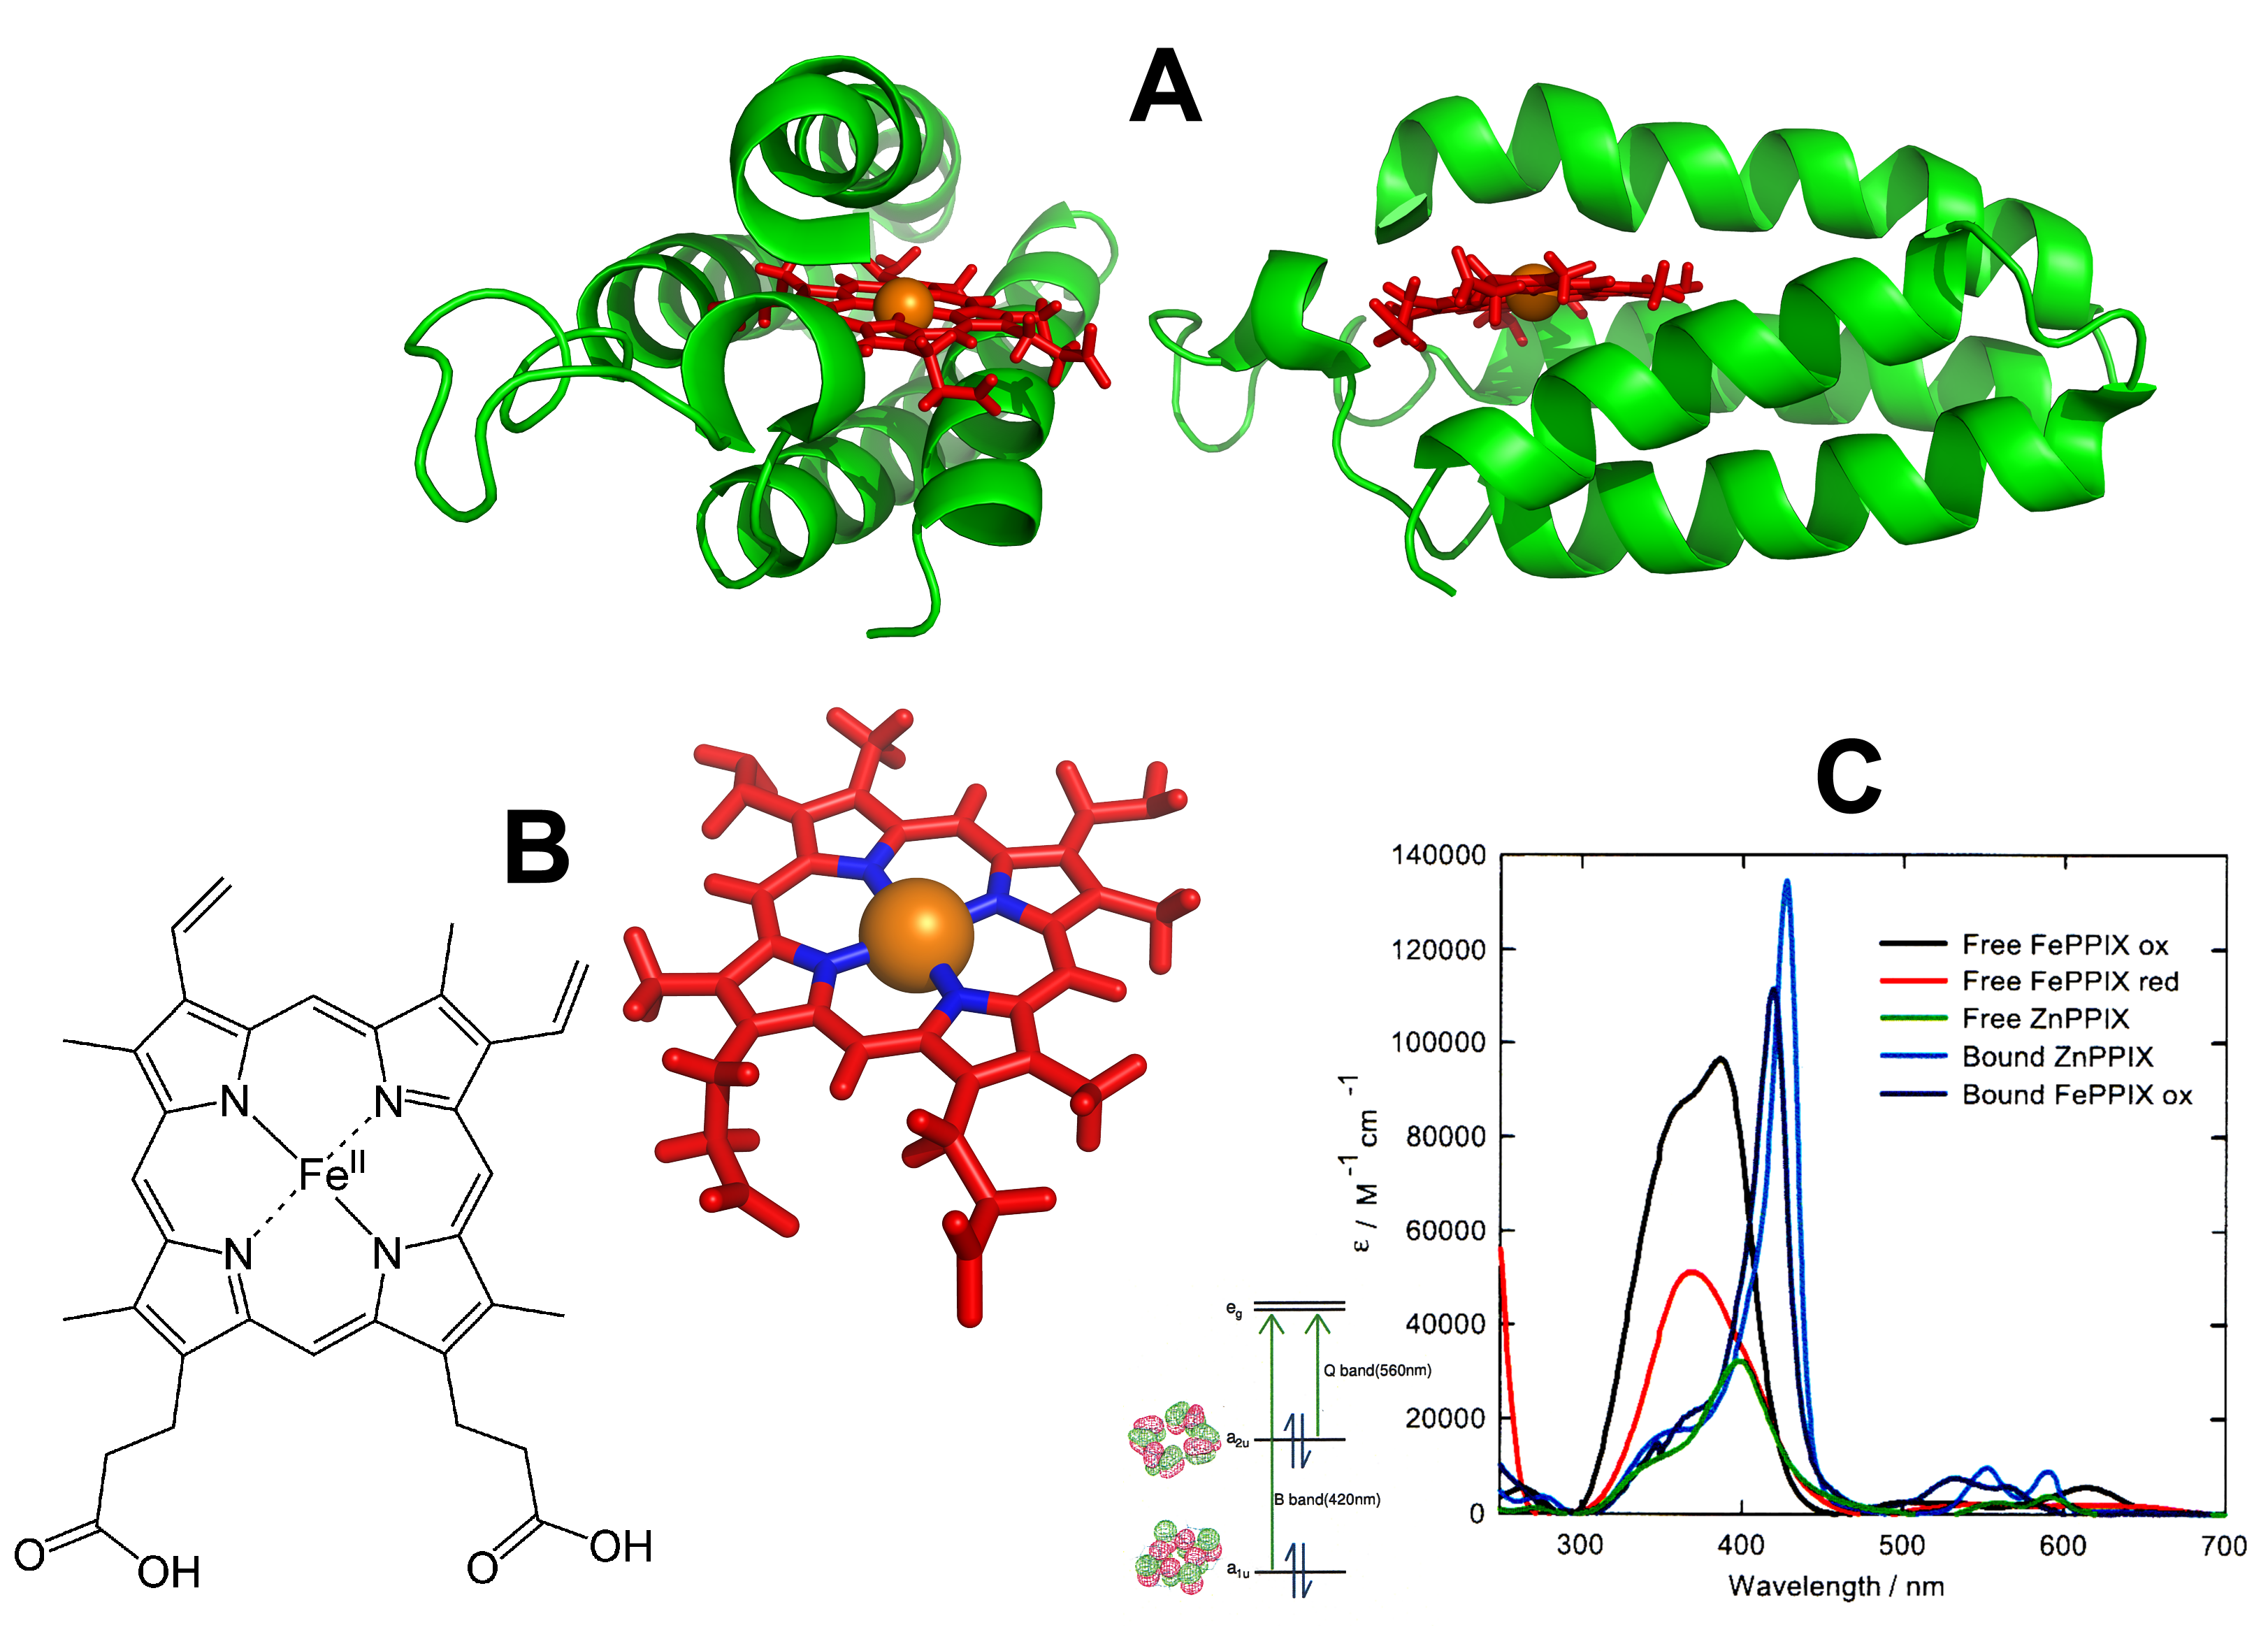
\includegraphics[width=137.4mm]{Images/haemStructure.png}
	\caption[Haem Structure]{A fancy image.}
	\label{fig:haemStructure}
\end{figure}
\end{verbatim}

\vspace{2ex}

\begin{figure}[!th]
	\centering
	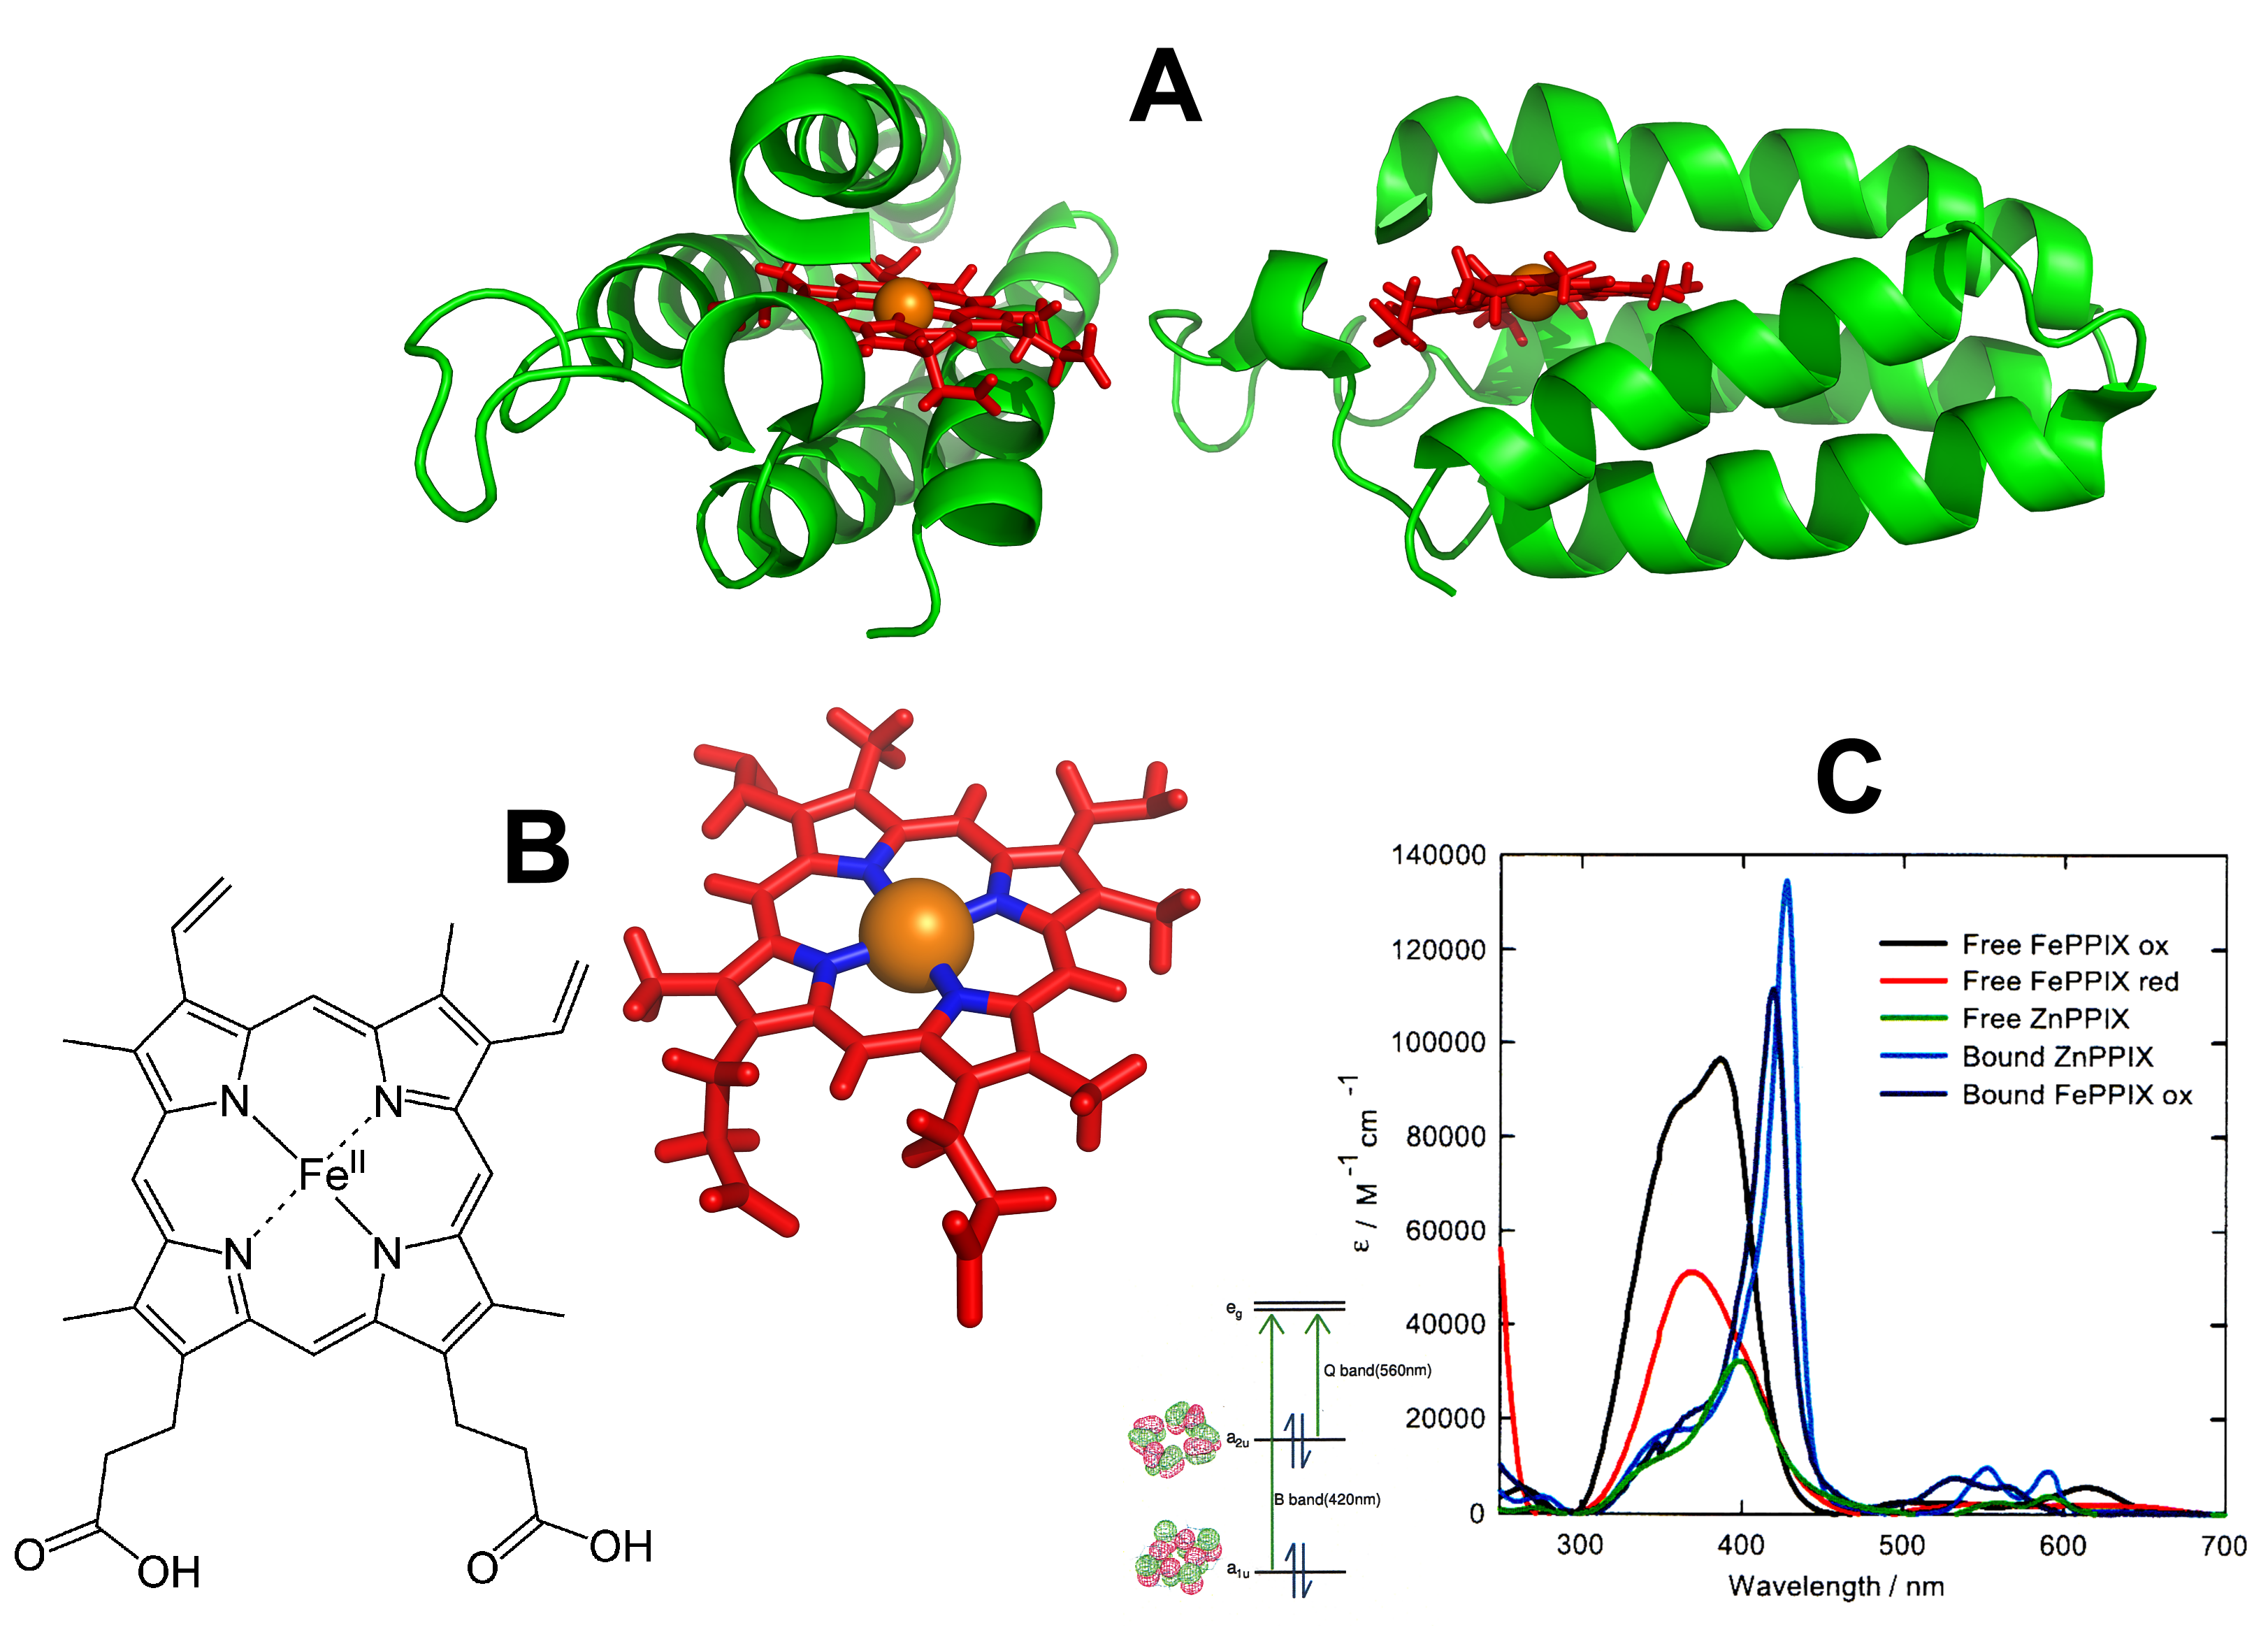
\includegraphics[width=137.4mm]{Images/haemStructure.png}
	\caption[Haem Structure]{A fancy image from Chris' Thesis.}
	\label{fig:haemStructure}
\end{figure}

In this example the command {\textbackslash}includegraphics tells LaTeX to look in the directory `Images' and incorporate the file called `haemStructure.png' into the final document while setting the width to 137.4mm.  This command can be used to resize a graphical file using the height or width parameter as shown. You must specify the units which can be pt, ex, em, mm, cm and so on. LaTeX recognises a very wide variety of standard units and graphics formats. The command is part of the graphicx package and so in the preamble you must include the command {\textbackslash}usepackage\{graphicx\}.

Many packages have been written to provide new commands. For example the `subfigure' package enables you to place separate images or files in the same figure side by side while giving them their own label. However, in this document we only concentrate on the very basics.

\section{Floating Environments}

Both tables and figures are examples of a `floating environments' which means LaTeX decides where to put them. 

The mysterious [!tbh] letters give guidance to LaTeX about roughly where the figure or table is  allowed to be, but in general they can move a long way from where you position them within your text file.  The letters in the square bracket can be t, h or b which stand for top, here or bottom.  If you don't specify any letters LaTeX defaults to [t].

LaTeX will always preserve the order in which figures appear.  If it cannot find a type setting solution, then it may move the float to it's own page, and combine it with other figures. If it still can't fit that in for some reason then it moves the float to the end of the document.  This has the effect of pushing all the remaining floating environments to the end of the document also.

The exclamation mark instructs LaTeX to ``try harder'' at putting the float where you told it to. Often you must play around to ensure the float positioning is acceptable, but usually this can be achieved by stretching or shrinking the image slightly using the size parameter, re-ordering text, judicial applications of the {\textbackslash}pagebreak command or by shouting loudly and slapping the computer monitor about. Note that it is better to resize the image using the original program that was used to create the image. Also using vector graphics can assist be useful (e.g. eps files) because they are designed to scale better.
\chapter{The Chapter on Making Chapters}
\label{sec:Chapters}

Right. LaTeX forces you to structure your document. There a series of simple commands for achieving this:

\vspace*{2ex}

{\textbackslash}chapter\{chapterName\}

{\textbackslash}section\{sectionName\}

{\textbackslash}subsection\{subsectionName\}

{\textbackslash}subsubsection\{subsubsectionName\}

\vspace*{2ex}

Easy enough. At the start of each chapter or section just issue one of these commands to name the section and LaTeX will present the chapter heading in the right style of font, which will be the same style of all the other heading names at that level of hierarchy throughout the document. In addition LaTeX assigns a number to that section. For example, this chapter was created using the command:

\vspace*{2ex}

{\textbackslash}chapter\{The Chapter on Making Chapters\} 

\vspace*{2ex}

LaTeX assigns the correct chapter number to each chapter in turn and then puts it in the table of contents, as you can see by looking at the table of contents! Easy.

\pagebreak
\section{The Section About Sections}
\label{sec:Section}
I think you're getting the hang of this. This section was created using the command {\textbackslash}section\{The Section About Sections\}. It appears in the table of contents as section \ref{sec:Section}.

\subsection{The Sub-Section About Sub-Sections}
\label{sec:SubSection}
Now you're really getting the hang of this. This subsection was created using the command {\textbackslash}subsection\{The Sub-Section About Sub-Sections\}. 

\subsubsection{The Sub-Sub-Section About Sub-Sub-Sections}
\label{sec:SubSubSection}
Now you're really getting the hang of this. but.. caught you out! This subsubsection doesn't have a number!  Ha Ha! It was created using the command {\textbackslash}subsubsection\{The Sub-Sub-Section About Sub-Sub-Sections\} in the same vein as all the other subsections/chapters etc. Here we have stopped the depth of the section numbering at the second level with the command:

\vspace*{2ex}

{\textbackslash}setcounter\{secnumdepth\}\{2\}

\vspace*{2ex}

Easy. WYSIWYM.  LaTeX does what you tell it to do. This is both a blessing and a curse.

\pagebreak
\section*{The Section About Sections That Don't Appear in the Table of Contents}
\label{sec:InvisibleSection}
Ok. Now we're throwing a spanner in the works. This section was created using the command:

\vspace*{2ex}

{\textbackslash}section*\{The Section About Sections That Don't Appear in the Table of Contents\}. 

\vspace*{2ex}

Notice how LaTeX has not assigned a number to the section and it doesn't appear in the table of contents. The effect of the * is to suppress the inclusion of a chapter, section or subsection in the automatic numbering. Easy. You can do this at any level. This is useful for things like prefaces, tables of contents or acknowledgements which you may or may not wish to have an entry in the main contents table. Up to you. It's your thesis. Don't just copy me.

\section{A Small Point About Numbering}

In this section notice how the numbering starts from where it left off before we suppressed the numbering on the previous section. Easy. WYSIWYM.
\pagebreak
\section{The Section About Internal Referencing}
\label{sec:InternalReferencing}

There are two related commands:

\vspace*{2ex}

{\textbackslash}label\{labelName\} 

{\textbackslash}ref\{labelName\}

\vspace*{2ex}


The {\textbackslash}label\{\} command allows you to create a label in a particular environment\footnote{That's right. Chapters, Sections and sub-sections etc are environments!}. The label won't appear in the final document. It's just a label which makes it easy to refer back to any particular environment elsewhere in the document. The {\textbackslash}ref\{\} command enables you to insert a reference anywhere in the document to any label in the document.  For example this is section \ref{sec:InternalReferencing}. The names you use in a label can be anything you like but musn't contain whitespace or special characters. I used the two commands:

\vspace*{2ex}

{\textbackslash}label\{sec:InternalReferencing\}

{\textbackslash}ref\{sec:InternalReferencing\}.

\vspace*{2ex}

The astute among you will realise that LaTeX has to read the document several times. Once to find the labels and then again to populate the references with the correct numbers. So you have to compile a latex document twice to get the referencing right. If there is a missing label or you refer to something that doesn't exist then latex inserts a convenient ? at that point. So hunting for queries is useful way of finding broken references. Latex issues warnings when it finds broken references.

As you create a document you will find yourself putting labels in all over the place so choose a sensible naming convention to help you remember the label names.

Each type of environment (equations, figures, tables, sections etc) has its own independent numbering system.  So when you choose your label name it's a good idea to have an identifier for that type of environment.  I have my own convention for label names which I use to help me remember references. E.g.   sec:SectionAboutCats. Eqn:EquationAboutCats,  Fig:FigureAboutCats and so on. This means you can differentiate between referring to the section or the figure more easily, even though they are about the same thing.

So Internal Referencing is a doddle. Easy!
\chapter{External Referencing}

Referencing is usually performed using a separate program called BibTex.  This program understands the file format .bib.

To create a reference within your document first you must create a .bib file by exporting your list of references from which ever referencing software you used, such as endnote, mendeley or whatever you use.

You can refer to an entry in the .bib file using the {\textbackslash}cite\{ref:Name\} command. the identifier `ref:Name' is the unique identifier which is the first line of each item included in your bibliography file.

For example, open the file LaTexCourseBib.bib in the bibliography directory. The first entry has the identifier `Horcas2007'.  This can be invoked as follows:


\begin{verbatim}
For example, this interesting fact\cite{Horcas2007}, is a cracking example.
\end{verbatim}

For example, this interesting fact\cite{Horcas2007}, is a cracking example.

During compilation latex and bibtex co-operate. During the first compilation latex generates a list of references that it needs.  During the second compilation bibtex populates the details from the .bib file into a shorter, ordered .bib file. The third compilation inserts markers at the right place in the main file and the fourth compilation generates the final list of references. Thus the compilation sequence is latex, bibtex, latex, latex.

The style of the referencing format can be changed using the command {\textbackslash}bibliographyStyle\{\}. e.g. the style used in this document is cjfthesisv1.bst which is invoked by 

\begin{verbatim}
\bibliographystyle{Bibliography/cjfthesisv1}
\end{verbatim}

The location of the list of references in the document is specified by issuing the {\textbackslash}bibliography\{\} command which also specifies the master bibliography file.

\begin{verbatim}
\bibliography{Bibliography/LaTeXCourseBib}
\end{verbatim}




\chapter{Organising Your Files}
One of the drawbacks of word is that the figures and tables are included within the document which becomes very very clunky quite quickly and once it reaches around 100Mb it becomes unwieldy and hard to export. One of that advantages of LaTeX is that the files are all text files and so are very light on resources and are easy to email around the place.

However, sometimes it can be difficult to navigate through a single text file, so if you had a huge document then it becomes difficult to find your way around.  One way of circumnavigating this problem is to break the file up into smaller files. As long as LaTeX knows where to look you can have a file for each logical sub-division of your document.

Therefore it is worth spending a bit of time at the beginning of a large project deciding how you wish to break up your LaTex Files and organise them neatly and tidily.  You can then tell LaTex where to look for the files using the following command:

\vspace*{2ex}
{\textbackslash}include\{fileName\}
\vspace*{2ex}

\pagebreak
\section{Linking a File}
We are now going to copy part of the tutorial file into a separate files and link it the main file.  Because this could go wrong it is sensible to back up tutorial.tex as something else. So save a copy called `tutorialOriginal.tex' for safe keeping. Then follow the following instructions.

\begin{enumerate}
\item Create a new file called MyFirstPage.tex
\item Select and Cut out the first chapter of Tutorial.Tex
\item Paste the first chapter into MyFirstPage.tex
\item Save both tutorial.tex and MyFirstPage.tex
\item Then add {\textbackslash}include\{MyFirstPage\} in tutorial.tex where the text used to be before you cut it out. We don't need to add the `.tex' because LaTeX can only include `.tex' files.
\item compile tutorial.tex and view the PDF
\end{enumerate}

The final PDF should look exactly the same as it was! except we now have a separate file for one of the chapters.

\pagebreak
\section{Creating A Class File}
We can also save our preamble in a separate file called a class file. This makes your main document much easier to understand.  To make it work we need to use the {\textbackslash}LoadClass\{\} command as follows: 

\begin{enumerate}
\item Create another new file and save it as TutorialStyle.cls
\item Copy the preamble of tutorial.tex into the new file. Starting with the {\textbackslash}documentclass{} command and copy right up to, but not including, the {\textbackslash}begin{document} command. Delete the preamble in the original document.
\item Save TutorialStyle.cls and tutorial.tex
\item Modify the first line of TutorialStyle.cls by replacing the word `document' with the word `Load'.
\item Add a new first line of tutorial.tex to use your new style class {\textbackslash}documentclass\{TutorialStyle\}
\item Save both files.
\end{enumerate}

\subsection{Sanity Check}

The first line of TutorialStyle.cls should now be:

\begin{verbatim}
\LoadClass[12pt, oneside, a4paper]{book}
\end{verbatim}
\vspace{2ex}

The first line of tutorial.tex should be:

\begin{verbatim}
\documentClass{TutorialStyle}
\end{verbatim}
\vspace{2ex}

We have just created what is called a style file. You can use this style file as a generic preamble for other documents as well. Compile tutorial.tex.  Nothing should have changed in the final PDF.


\pagebreak
\section{The Structure of this Document}

Lets now look at how I've organised this document. It is identical to my thesis because it started out life as my thesis. I usurped the structure and simply replaced the headings and content to make a kind of reference manual for this introductory course. This document therefore is three things:

\begin{enumerate}
\item An example thesis structure to work from.
\item The LaTeX files which were used to create it can be used as a template for a thesis.
\item It is also a convenient introductory latex manual!
\end{enumerate}

\vspace*{2ex}
Groovy huh?

\section{The Master File}

There is a master file where LaTeX begins the compilation procedure. This contains the {\textbackslash}documentclass command needed to set the ball rolling. Within the file there are a series of {\textbackslash}include\{\} commands, one for each Chapter, which tell LaTeX where to find the files containing each chapter.

The subfiles cannot be compiled on their own because they do not contain the {\textbackslash}documentclass, {\textbackslash}begin\{document\} or {\textbackslash}end\{document\} commands. Lets us look in more detail at the master file and we will learn some new LaTeX commands.

\singlespacing
\pagebreak
\begin{verbatim}
\documentclass{Style/LatexCourseStyle}

\begin{document}
\setcounter{secnumdepth}{2}
\setcounter{tocdepth}{1}

\frontmatter
\onehalfspacing
\include{Frontmatter/Titlepage}
\include{Frontmatter/Declaration}
\include{Frontmatter/Acknowledgements}
\include{Frontmatter/Summary}
\include{Frontmatter/Abbreviations}
\tableofcontents
\listoftables
\listoffigures

\mainmatter
\renewcommand{\sectionmark}[1]{\markright{\thesection \ #1}{}}
\include{Chapters/Overview}
\include{Chapters/MyFirstPage}
\include{Chapters/Lists}
\include{Chapters/mathsEquations}
\include{Chapters/ChemicalEquations}
\include{Chapters/Tables}
\include{Chapters/Figures}
\include{Chapters/Sectioning}
\include{Chapters/externalReferencing}
\include{Chapters/ThesisTemplateMainFile}
%\include{Chapters/ChapterThatIsNotCompiled}

\appendix
%\include{Appendices/UsefulWebsites}

\singlespacing

\backmatter
\addcontentsline{toc}{chapter}{References}
\bibliographystyle{Bibliography/cjfthesisv1}
\renewcommand{\bibname}{References}
\bibliography{Bibliography/LatexCourseBib}

\end{document}
\end{verbatim}
\onehalfspacing
\pagebreak

\section{Analysing the Master File}
Let us go through this file and observe the new commands. Most of it is self-explanatory.

\begin{verbatim}
\documentclass{Style/LaTeXCourseStyle}
\end{verbatim}

This command tells latex that the document class is the one defined in the the style file ''LaTeXCourseStyle'', which is in the sub directory ''style''.  Easy.

\begin{verbatim}
\setcounter{secnumdepth}{2}
\setcounter{tocdepth}{1}
\end{verbatim}

The first of these commands tells latex that the section depth number is 2. I.E. throughout the document only bother numbering sections, subsections and subsubsections down to the second level (such as section 1.2.3). The second command tells latex to only build the table of contents from section numbers down to the first level i.e. 1.1.  Easy enough.

The command {\textbackslash}frontmatter is exclusive to the book class, on which this style is based, and tells latex that within this section to number the pages using roman numerals, and not to include these numbers in the table of contents, just like in a book. The {\textbackslash}mainmatter and {\textbackslash}backmatter commands similarly delineate the other sections of the document.  

Childs play.  How long would it take you to figure out how to do that in word???? No idea. I've never tried.

Note that these rather cool commands are not available in every single class. So for a paper you would use the article class where such compartmentalisation of your document is not appropriate. In fact you can often download latex templates from the journal to wish to submit your paper, which is why I concentrate on the thesis template in this course.

\begin{verbatim}
\onehalfspacing
\end{verbatim}

Is obvious. ''From this point forward use line spacing of one and a half lines please. Thank you.'' How many hours have you spent clicking on paragraph indentations for each separate paragraphs in word? Nightmare. Want to change the standard in the whole document? Not a chance in word. In latex, you can do it with a single word, carefully placed in the master file.

\begin{verbatim}
\include{Frontmatter/Titlepage}
\include{Frontmatter/Declaration}
\include{Frontmatter/Acknowledgements}
\include{Frontmatter/Summary}
\include{Frontmatter/Abbreviations}
\end{verbatim}

The {\textbackslash}include\{\} command tells latex to include the specified .tex file at this point.  Thus it is a simple matter to break up a large document into sub components.  I have written each part of the front matter in a separate file and then grouped all the front matter into one directory called: Frontmatter.

See how the directory structure of my files reflects the structure of my book?

\begin{verbatim}
\tableofcontents
\listoftables
\listoffigures
\end{verbatim}

Again. This is easy. These commands mean: ''Please scan through the whole document and build for me a table of contents, a list of tables, a list of figures and then write down the entries along side their section numbers (as I have them ordered in this version of the document), as well as the page numbers on which they appear and create a nice little summary table and add them to the front matter of my document. Thanks.''.

How does latex do this?  remember the idea of environments?  Well each table, figure, equation etc is a defined environment.  LaTeX just counts them up and assigns numbers starting wherever you want and builds a table.  You can tell latex to ignore individual sections if you want to.

You can also control the look and feel of your table of contents with subtley and grace. Do you want to fill the white space with lines of dots to aid readability, even though the chapter titles are all different lengths? page numbers? How deep should the TOC been?  etc etc etc. How to do this is beyond the scope of this course, but now you know about it, go look it up. easy as $\pi$.

Ok.

Main matter we've done.

\begin{verbatim}
\renewcommand{\sectionmark}[1]{\markright{\thesection \ #1}{}}
\end{verbatim}

This command tells latex to 'renewcommand', i.e. change the meaning of the following command from this point in the document forward, over-riding previous definitions.
\begin{verbatim}
\sectionmark}[1]{\markright{\thesection \ #1}{}
\end{verbatim}

Is latex speak for ``please write the section heading at the top right hand side of each page. thanks''. This works in conjunction with a command in the style file which we'll talk about later. You have to tell latex to switch on headings as well as where to put them.

\begin{verbatim}
\include{Chapters/Overview}
\include{Chapters/MyFirstPage}
\include{Chapters/Lists}
\include{Chapters/mathsEquations}
\include{Chapters/ChemicalEquations}
\include{Chapters/Tables}
\include{Chapters/Figures}
\include{Chapters/Sectioning}
\include{Chapters/externalReferencing}
\include{Chapters/ThesisTemplateMainFile}
%\include{Chapters/ChapterThatIsNotCompiled}
\end{verbatim}

This is the include command again. You will notice that one of the include lines is commented out. This is a handy trick to only build certain parts of my thesis. Which can be useful if individual chapters are being reviewed.

\pagebreak

\begin{verbatim}
\appendix
%\include{Appendices/UsefulWebsites}

\singlespacing

\backmatter
\addcontentsline{toc}{chapter}{References}
\bibliographystyle{Bibliography/cjfthesisv1}
\renewcommand{\bibname}{References}
\bibliography{Bibliography/LatexCourseBib}
\end{verbatim}

The rest is easy. {\textbackslash}Appendix means we are in the appendix now and start labelling sections with A.1.2 instead of 1.2.3.  

{\textbackslash}addcontentsline means forcibly insert a contents line about the references into the contents table. 

{\textbackslash}\{bibliographystyle\{Bibliography/cjfthesisv1\}\} means use the biblography style defined in the file cjfthesisv1. Defining a bibliography style will be covered later if we have time. This is where you specify how the references will appear (names, journals, full stops, commas etc).

{\textbackslash}renewcommand\{{\textbackslash}bibname\}\{References\} means: rename the bibliography chapter as `References'

{\textbackslash}biblography means add the following bibliography.  You can reference entries in this bibliography file very easily.

The astute among you will realise that LaTeX will have to read the document several times before it can be compiled with all the references.  Hey ho. No problem. You can go and have a cuppa while LaTeX does your references for you in the style of your favorite journal... nice.




%\include{Chapters/ChapterThatIsNotCompiled}

\appendix
%\include{Appendices/UsefulWebsites}

\singlespacing

\backmatter
\addcontentsline{toc}{chapter}{References}
\bibliographystyle{Bibliography/cjfthesisv1}
\renewcommand{\bibname}{References}
\bibliography{Bibliography/LatexCourseBib}

\end{document}
\end{verbatim}
\onehalfspacing
\pagebreak

\section{Analysing the Master File}
Let us go through this file and observe the new commands. Most of it is self-explanatory.

\begin{verbatim}
\documentclass{Style/LaTeXCourseStyle}
\end{verbatim}

This command tells latex that the document class is the one defined in the the style file ''LaTeXCourseStyle'', which is in the sub directory ''style''.  Easy.

\begin{verbatim}
\setcounter{secnumdepth}{2}
\setcounter{tocdepth}{1}
\end{verbatim}

The first of these commands tells latex that the section depth number is 2. I.E. throughout the document only bother numbering sections, subsections and subsubsections down to the second level (such as section 1.2.3). The second command tells latex to only build the table of contents from section numbers down to the first level i.e. 1.1.  Easy enough.

The command {\textbackslash}frontmatter is exclusive to the book class, on which this style is based, and tells latex that within this section to number the pages using roman numerals, and not to include these numbers in the table of contents, just like in a book. The {\textbackslash}mainmatter and {\textbackslash}backmatter commands similarly delineate the other sections of the document.  

Childs play.  How long would it take you to figure out how to do that in word???? No idea. I've never tried.

Note that these rather cool commands are not available in every single class. So for a paper you would use the article class where such compartmentalisation of your document is not appropriate. In fact you can often download latex templates from the journal to wish to submit your paper, which is why I concentrate on the thesis template in this course.

\begin{verbatim}
\onehalfspacing
\end{verbatim}

Is obvious. ''From this point forward use line spacing of one and a half lines please. Thank you.'' How many hours have you spent clicking on paragraph indentations for each separate paragraphs in word? Nightmare. Want to change the standard in the whole document? Not a chance in word. In latex, you can do it with a single word, carefully placed in the master file.

\begin{verbatim}
\thispagestyle{empty}

\begin{center}
\vspace*{\stretch{1}}

\hrule height 2pt
\vspace*{2ex}
{\Huge\textbf{Towards the Ability to Make Super Duper LaTeX Documents}\par}
\vspace*{2ex}
\hrule height 2pt
\vspace*{10ex}
{
\includegraphics[height=40mm]{Images/UnivShield}\par}
\vspace*{10ex}
{\large\textbf{Christopher~James~Forman}\par}
\vspace*{2ex}
{\large{Department Of Chemistry}\par}
\vspace*{2ex}
{\large{University of Cambridge}\par}
\vspace*{5ex}
{\large{This dissertation is submitted for the degree of \textit{Doctor of Philosophy}}\par}
\vspace*{5ex}
{\large{\today}\par}

\vspace*{\stretch{2}}
\end{center}
\chapter*{Declaration}

\vfill

This dissertation is the result of my own work and includes nothing which is the outcome of work done in collaboration except where specifically indicated in the text. It is not substantially the same as any that I have submitted for a degree or diploma or other qualification at any other University and no part has already been, or is concurrently being, submitted for any degree, diploma, or other qualification. It does not exceed 60,000 words, including tables, footnotes, bibliography and appendices.\par

\vspace{10ex}

\begin{flushright}
Signature: \rule[0pt]{60mm}{0.5pt}

\vspace{5ex}

Date: \rule[0pt]{60mm}{0.5pt}
\end{flushright}

\vfill
\chapter*{Acknowledgments}
\subsection*{Family}
Mum. Dad. Pet Dog.

\subsection*{Scientific Collaborations}
Dr A.N.Other at uni of blah for samples and instrument time etc. My Amazing Lab Chums.

\subsection*{Scientific Support}
My amazing lab chums.

\subsection*{General Assistance}
Cleaner, My amazing lab chums.

\subsection*{Financial Support}
Bank, Tax payer. My amazing lab chums.

\subsection*{Moral Support}
My Amazing Lab chums.

\subsection*{Academic Inspiration}
Netwon, My super. My Amazing Lab Chums.

\subsection*{Everyone else}
My Amazing Lab Chums.

\chapter*{Summary}
This document is a handbook for introducing you to LaTeX. It contains a bit of background about the history and philosophy of LaTeX.  However, it concentrates on providing a guided practical introduction to the basic techniques such as 
\begin{itemize}
\item Lists
\item Mathematical and chemical equations
\item Tables
\item Figures
\item Chapters and Sections
\item Linking to other files in large documents
\item Referencing
\end{itemize}

The handbook is also presented in the style of a thesis. This means that source files provided on the introductory course and available from the department web page are a convenient template for a thesis.

More details on specific aspects of LaTeX can be found at the departmental LaTeX page which can be found here:

 http://www-ch-int.ch.private.cam.ac.uk/latex/about

\chapter*{Abbreviations}

\begin{longtable}{r >{\rule{0pt}{3ex}}l<{\rule[-1.5ex]{0pt}{0pt}}}
ADP & Adenosine Diphosphate\\
(nc/c)AFM & (non-contact/conducting) Atomic Force Microscopy\\
ATP & Adenosine Triphosphate \\
\end{longtable}
\end{verbatim}

The {\textbackslash}include\{\} command tells latex to include the specified .tex file at this point.  Thus it is a simple matter to break up a large document into sub components.  I have written each part of the front matter in a separate file and then grouped all the front matter into one directory called: Frontmatter.

See how the directory structure of my files reflects the structure of my book?

\begin{verbatim}
\tableofcontents
\listoftables
\listoffigures
\end{verbatim}

Again. This is easy. These commands mean: ''Please scan through the whole document and build for me a table of contents, a list of tables, a list of figures and then write down the entries along side their section numbers (as I have them ordered in this version of the document), as well as the page numbers on which they appear and create a nice little summary table and add them to the front matter of my document. Thanks.''.

How does latex do this?  remember the idea of environments?  Well each table, figure, equation etc is a defined environment.  LaTeX just counts them up and assigns numbers starting wherever you want and builds a table.  You can tell latex to ignore individual sections if you want to.

You can also control the look and feel of your table of contents with subtley and grace. Do you want to fill the white space with lines of dots to aid readability, even though the chapter titles are all different lengths? page numbers? How deep should the TOC been?  etc etc etc. How to do this is beyond the scope of this course, but now you know about it, go look it up. easy as $\pi$.

Ok.

Main matter we've done.

\begin{verbatim}
\renewcommand{\sectionmark}[1]{\markright{\thesection \ #1}{}}
\end{verbatim}

This command tells latex to 'renewcommand', i.e. change the meaning of the following command from this point in the document forward, over-riding previous definitions.
\begin{verbatim}
\sectionmark}[1]{\markright{\thesection \ #1}{}
\end{verbatim}

Is latex speak for ``please write the section heading at the top right hand side of each page. thanks''. This works in conjunction with a command in the style file which we'll talk about later. You have to tell latex to switch on headings as well as where to put them.

\begin{verbatim}
\chapter{Overview}
\label{chap:overview}
\section{LaTeX: The answer to everything.}
LaTeX is typsetting program that takes an input file of marked up text and then, with a user defined set of rules, typesets a beautifully crafted output file that can be easily printed (e.g. a pdf). 

\subsection{Advantages}

The advantages of this method are manifold:

\begin{itemize}

\item Use any text editor to view the source document.
\item More time can be spent working on the content and not worrying about how text or figures interact in the layout until later on.
\item LaTeX uses consistent rules throughout a document
\item LaTeX sorts out basic typesetting automatically
\item Changes can be introduced globally with very little effort
\item Document structure is explicit
\item Documents can be professionally typeset and look great
\item You are forced to structure your documents correctly.
\item Mathematical equations, like $E=mc^2$ or $\imath\hbar\frac{\partial}{\partial t}\Phi (x, t) = \hat{H}\Phi (x, t)$ can be produced almost as fast as typing (if you know the commands!).
\end{itemize}

\subsection{Disadvantages}
The disadvanatges of this method are also manifold:
\begin{itemize}
\item You don't see the output as you go.
\item Steep learning curve.
\item Documents are harder to edit by a second author (unless they are adept at LaTeX too). This can be mitigated using version control, which makes group authoring processes superior to word.
\item The program never works quite the way you want it to and learning how to influence it can be problematic and subtle.
\item Although intended to save work the principle of 'conservation of work' means that you simply transform problems associated with WYSISYG approaches to problems associated with WYSIWYM approaches!
\item You can go blind trying to determine the difference between wiggly and smooth brackets if your editors font isn't large enough.
\end{itemize}

\subsection{On balance?}
If it's so rubbish, why use LaTeX?

\begin{itemize}
\item Large documents are much more easily handled. 
\item In general it is quicker to debug a LaTeX document than typeset an entire thesis manually. 
\item Technical information such as tables, equations and figures are integrated much more smoothly than with word.
\end{itemize}

\section{How does it work?}

The raw text is interspersed with commands, preceded by a \textbackslash, which tell LaTeX what to do with the text. For example you can \textbf{make it bold}, \emph{italic}, or \underline{underlined} with the commands {\textbackslash}textbf\{\}, {\textbackslash}emph\{\} or {\textbackslash}underlined\{\}. More on commands in a moment...



\chapter{My First Page}

\section{The Very Beginning}
The very simplest LaTeX document might look like this:

\begin{verbatim}
\documentclass[a4paper,12pt]{article}
\begin{document}
Hello World.
\end{document}
\end{verbatim}

\pagebreak
\thispagestyle{empty}
Hello World.
\pagebreak
\subsection{Break Down}
What's all the gobbledegook around my simple message???

In LaTeX we intersperse text and commands.  Commands are preceded by a \textbackslash. For example the first line in a LaTeX document \underline{\textbf{\emph{must}}} be:

\begin{verbatim}
\documentclass[options]{class}
\end{verbatim}

Where the word ''class'' may be substituted for one of many things such as: article, proc, minimal, report, book, letter, memoir, slides, beamer.

Similarly, and completely generally in LaTeX speak, the square brackets denote the existence of optional parameters. Each individual command can take its own parameters and for the ''{\textbackslash}documentclass'' command there are options for controlling font size, font family, landscape, oneside, twosided, page size and so on. These options will persist throughout the entire document. For example the document class command for this document, (which is likely to be like the one you would use for a thesis), would be:

\begin{verbatim}
\documentclass[12pt, oneside, a4paper]{book}
\end{verbatim}

Other options include:

\begin{itemize}
\item {10pt, 11pt, 12pt (default is 10pt).}
\item {letterpaper, legalpaper, a4paper, executivepaper, a5paper, b5paper}
\end{itemize}
and so on.

\pagebreak
\section{Can I start typing please?}

After we have set up the document we can start actual work on our document. So we must tell LaTeX that what follows is to be interpreted as a document.  The command {\textbackslash}begin can take many different parameters and is a command to enter what is known, in LaTeX speak, as 'an environment'. Thus the commands:
\begin{verbatim}
\begin{document}

\end{document}
\end{verbatim}

tells LaTeX to enter and leave the document environment, and thus constitute the outer limits of our document file. Other environments include the equation environment, the itemize environment, the figure environment and so on. These will be encountered in due course.

Every part of the LaTeX file is therefore within an environment of specific type and the content within each environment consists of commands or text.

That's basically it.

So let's get on with it shall we...

\pagebreak
\section{The ground rules}
\begin{quote}
Hold on, hold on, hold on my son.

First the lessons.

Then the fun!
\end{quote}
Dr Seuss.

\subsection{Spaces}
Whitespace characters, such as blank or tab, are treated uniformly as space by LaTeX. Several consecutive whitespace characters are treated as one single space. Whitespace at the start of a line is generally ignored, and a single line break is treated as whitespace. An empty line between two lines of text defines the end of a paragraph. Several empty lines are treated the same as one empty line. The text below is an example.

\begin{verbatim}
It does not matter whether you
enter one or several             spaces
after a word. The final result will be typeset beautifully
according    to     precise rules.




An empty line starts a new
paragraph. Note the indentation on the first line of the paragraph, 
except at the beginning of the section. 
\end{verbatim}

\vspace*{2ex}
\vspace*{2ex}

It does not matter whether you
enter one or several             spaces
after a word. The final result will be typeset beautifully
according    to     specific rules.




An empty line starts a new
paragraph. Note the indentation on the first line of the paragraph, except at the beginning of the section. 

\pagebreak
\subsection{Special Characters}
The symbols 

\# \$ \% \textasciicircum{} \& \_ \{ \} \~{} \textbackslash

are reserved characters that either have a special meaning under LaTeX or are unavailable in all the fonts. If you enter them directly in your text, they will normally not print, but rather make LaTeX do strange things.

To overide the special meanings of these symbols and allow them to produced within your text you may use the following sequences:
\begin{verbatim}
\# \$ \% \textasciicircum{} \& \_ \{ \} \~{} \textbackslash
\end{verbatim}

Other symbols and many more can be printed with special commands in mathematical formulae or as accents.

The backslash character '\textbackslash' cannot be entered by adding another backslash in front of it ( \textbackslash\textbackslash); because this sequence means ''linebreak''.

The command \textbackslash\~{}\{\} produces a tilde which is placed over the next letter. For example \textbackslash\~{}\{n\} gives \~{n}. To produce just the character \~{}, use \textbackslash\~{}\{\} which places a \~{} over an empty box.

Similarly, the command \textbackslash\textasciicircum{} produces a hat over the next character, for example \textbackslash\textasciicircum\{o\} produces \^{o}.

\pagebreak
\section{Preamble}
After the {\textbackslash}documentclass command we add ''preamble''. Here we load special features that we will use throughout our document to expand on the basic capabilities of LaTex. These are contained in units called ''packages'' which we can tell our LaTeX compiler to download by using the command ''{\textbackslash}include\{packageName\}''. 

There are many repositories of such packages on the web. Your compiler generally knows where to look and most standard packages are included with any install. For example, to include a special set of typesetting instructions to handle chemical equations we can grow our simple document with a single command like this:

\begin{verbatim}
\documentclass[a4paper,12pt]{article}
\usepackage[version=3]{mhchem}
\begin{document}
Hello World!

We all need \ce{H2O}.

I'm less fussed about \ce{^{235}_{92}U+}.

\end{document}
\end{verbatim}

\vspace{2ex}

\pagebreak
\thispagestyle{empty}
Hello World!

We all need \ce{H2O}.

I'm less fussed about \ce{^{235}_{92}U+}.
\pagebreak

Here we have loaded a package called: "`mhchem"' which took the option ''[version=3]''. This is a package for drawing chemical equations easily and it has it's own instruction manual which you can follow easily. It is included in the bundle of files for this course.

Other things we can do in the premable within LaTeX are to redefine existing commands or create our own personal commands. These can be stored in a file called the 'style file' which we can load at the beginning of our document, in place of our documentclass. More about this later on...


\subsection{Comments}
It is often useful to comment your LaTeX documents. You can leave yourself amusing, sarcastic messages that won't get printed out in the final document. Use this to make your own notes as the course progresses.

To get a comment use the \% command, which tells LaTeX to ignore the rest of the line, the line break and all the white space at the beginning of the next line, for example, we may add to our continually evolving document...

\begin{verbatim}
\documentclass[a4paper,12pt]{article}
\usepackage[version=3]{mhchem}
\begin{document}
Hello World!

%All humans need water and I would like 
%to include this concept in my arguments.
We all need \ce{H2O}.

%Uranium 235 is toxic, which is why I don't want to consume it... 
I'm less fussed about \ce{^{235}_{92}U+}.

\end{document}
\end{verbatim}

\vspace{4ex}
Hello World!

%All humans need water and I would like to include this concept in my arguments.
We all need \ce{H2O}.

%Uranium 235 is toxic, which is why I don't want to consume it... 
I'm less fussed about \ce{^{235}_{92}U+}.

\pagebreak
\section{Compiling}
Once the document is finished you can compile it. Your compiler will depend on the platform that you use. In the PWF we are using winEDT to edit the documents (a LaTeX front end) and texlive2008 which is the compiler itself. I use MiKTex and the front end texCenter.  There is no need to use a front end. If you prefer you can use a simple text editor and a command line.

the recommended distributions are:
\begin{itemize}
\item MiKTeX or TeX Live for Windows
\item TeX Live for Unix/Linux
\item MacTeX or TeX Live for Mac OS.
\end{itemize}

Once you have installed your software and got it working, written your source code and tried to compile it, there will nearly always be something wrong with your file. 

Any errors will be highlighted in the console window or error output box of your front end.  Some front ends dump the running commentary which LaTeX produces into a text file for easy reading afterwards.

In a compile attempt (successful or otherwise) LaTeX may produce the following files:

projectname.aux

projectname.bbl

projectname.lof

projectname.lot

projectname.txt

projectname.toc

projectname.dvi

These are interim files (toc= table of contents, bbl = bibliography etc). To be honest I have no idea what half of these things contain.  You only need the .tex file and a compiler with the right packages installed to produce them again.

Some versions of LaTeX only produce DVI files and you then need to convert the dvi file to a PDF or download a dvi viewer. You can also convert DVI files to PS files and then view them.  The good thing about front ends is that you can set them up to produce PDFs directly.

OK. So we have now produced a silly document but we understand it.  Now lets get on with learning how to make our own documents.



\chapter{Lists}
Lists are great.  The command {\textbackslash}begin\{\} can be used to enter a list environment.  For example:

\begin{verbatim}
\begin{itemize}
\item cat
\item dog
\item horse
\end{itemize}
\end{verbatim}

Produces:

\begin{itemize}
\item cat
\item dog
\item horse
\end{itemize}

\pagebreak
We can also replace the bullet points with numbers using the enumerate keyword.

\begin{verbatim}
\begin{enumerate}
\item cat
\item dog
\item horse
\end{enumerate}
\end{verbatim}

\begin{enumerate}
\item cat
\item dog
\item horse
\end{enumerate}

\pagebreak
and we can use the description keyword which does this:
\begin{verbatim}
\begin{description}
\item[Cat] a lovely furry creature with a cute nose and whiskers.
\item[Dog] Another furry creature that smells rather well; 
           its olfactory power stems from its nasal dampness.
\item [Horse] A large stinky creature with sideways facing eyes.
\end{description}
\end{verbatim}

\begin{description}
\item[Cat] a lovely furry creature with a cute nose and whiskers.
\item[Dog] Another furry creature that smells rather well; its olfactory power stems from its nasal dampness.
\item [Horse] A large stinky creature with sideways facing eyes.
\end{description}
\chapter{Maths Equations}

\section{Producing Beautiful Looking Mathematics}

One of the best features about LaTeX is `maths mode'.  For example the schrodinger equation can be produced as follows:

\vspace*{2ex}

\begin{center}
\begin{math}
\imath\hbar\frac{\partial}{\partial t}\Phi (x, t) = \hat{H}\Phi (x, t)
\end{math}
\end{center}

\vspace*{2ex}

\begin{verbatim}
\begin{math}
\imath\hbar\frac{\partial}{\partial t}\Phi(x,t)=\hat{H}\Phi(x,t)
\end{math}
\end{verbatim}

There are a number of ways to switch on maths mode.  The first, as above, is with the {\textbackslash}begin\{math\} environment. You can also enter mathmode inline using the \$ symbol. For example typing in \$y=ax\textasciicircum{}2+bx+c\$ yields $y=ax^2+bx+c$.  Another way is to enter the equation environment which enables you to number equations so you can then refer to them later in the text.

\begin{equation}
y(t)= \sin \left(\frac{{\alpha}t}{2\pi} + \phi_0\right)
\label{eqn:MadeUpNonsense}
\end{equation}

\vspace*{2ex}
\begin{verbatim}
\begin{equation}
y(t)= \sin \left(\frac{{\alpha}t}{2\pi} + \phi_0\right)
\end{equation}
\end{verbatim}.

\section{Basic Maths Mode}
Once in maths mode there is a kind of text based code for writing down your equations.  Here are the most basic symbols to get you going.
\begin{center}
\begin{tabular}{cc}
\toprule
Final Result & LaTeX Code \\
\cmidrule(){1-2}
$a+b$ & a+b \\
$a-b$ & a-b \\
$ab$ & ab \\
$a*b$ & a*b \\
$a \times b$ & a {\textbackslash}times b \\
$a \cdot b$ & a {\textbackslash}cdot b \\
$\frac{a}{b}$ & {\textbackslash}frac\{a\}\{b\} \\ 
$a^b$ & a\textasciicircum{}b \\
$a_b$ & a\_b \\
$\sin a$ & {\textbackslash}sin a  (same for cos, tan)\\
$ sin a$ & sin a \\
$\sqrt{a}$ & {\textbackslash}sqrt\{a\} \\
$\left( a \right) $ & {\textbackslash}left( a {\textbackslash}right)\\ 
$\left[ a \right]$ & {\textbackslash}left[ a {\textbackslash}right]\\ 
$\alpha$ & {\textbackslash}alpha \\
$\pi$ & {\textbackslash}pi \\
\bottomrule
\end{tabular}
\end{center}

A full treatise on maths mode is not practical here. There are lots of online tutorials and summaries of symbols. It just takes a bit of practice and you can build up equations really easily. It's straight forward to learn new stuff once you've done it a few times.

\pagebreak
\section{Equation Arrays}
Sometimes you need to arrange several equations vertically, referencing individual lines separately and aligning the equations on the $=$ sign. This can be achieved with equation arrays as follows:

\begin{eqnarray}
A\left( x\right) & = & \frac{x^2+2x+1}{x+1} \\
& = & \frac{\left(x+1\right)\left(x+1\right)}{x+1} \nonumber\\
& = & x+1 \nonumber\\
B(x,t) & = & \frac{e^{\left(\imath\omega_0 t + kx\right)}}{4\pi\epsilon_0}
\end{eqnarray}

\begin{verbatim}
\begin{eqnarray}
A\left( x\right) & = & \frac{x^2+2x+1}{1+x} \\
& = & \frac{\left(x+1\right)\left(x+1\right)}{1+x} \nonumber\\
& = & x+1 \nonumber\\
B(x,t) & = & \frac{e^{\left(\imath\omega_0 t + kx\right)}}{4\pi\epsilon_0}
\end{eqnarray}
\end{verbatim}

\begin{itemize}
\item Note the \& symbols. This tells LaTeX where to align the equations. There must be the same number of \& symbols in each line.
\item Note the \textbackslash\textbackslash ~at the end of each line except the last one. This symbol tells LaTeX to add another row in the array.  If you put it on the last line you get an empty row at the bottom of the array.
\item Note the {\textbackslash}nonumber command which suppresses line numbering for that line.
\item Note that equation number carries on from equation \ref{eqn:MadeUpNonsense} in the previous section.
\end{itemize}

\section{Maths Packages}

Maths mode comes as standard in LaTeX, however you can download packages that buff up your maths symbol set. For example neat vector notation comes in the package `vector'. e.g. {\textbackslash}uuvec\{T\} yields $\uuvec{T}$.

\begin{verbatim}
\usepackage{amssymb}
\usepackage{amsmath}
\usepackage{vector}
\end{verbatim}


\chapter{Chemical Equations}
The mhchem package means you can do basic stuff very easily using {\textbackslash}ce\{\}. For example:

\vspace{2ex}
\begin{verbatim}
\ce{CO2 + C -> 2CO}
\ce{CO2 + C <- 2CO}
\ce{CO2 + C <=> 2CO}
\ce{A-B=C#D\sbond E\dbond F\tbond G}
\end{verbatim}
\vspace{2ex}
\begin{center}
\ce{CO2 + C -> 2CO}

\ce{CO2 + C <- 2CO}

\ce{CO2 + C <=> 2CO}

\ce{A-B=C#D\sbond E\dbond F\tbond G}
\end{center}

\vspace{2ex}
You can also use math mode within chemical equations.
\vspace{2ex}

\begin{center}
\ce{$x\,$ Na(NH4)HPO4 ->[\Delta] (NaPO3)_{$x$} + $x\,$ NH3 ^ + $x\,$ H2O}
\end{center}

\begin{verbatim}
\ce{$x\,$ Na(NH4)HPO4 ->[\Delta](NaPO3)_{$x$} + $x\,$ NH3 ^ + $x\,$ H2O}
\end{verbatim}

And you can number chemical reactions as well by using the math mode equation environment.

\begin{equation}
\ce{CO2 + C <=> 2CO}
\end{equation}

\begin{verbatim}
\begin{equation}
\ce{CO2 + C <=> 2CO}
\end{equation}
\end{verbatim}

However, this will number mathematical and chemical equations using the same number system. There is a discussion in the mhchem pdf which shows you how to number chemical and mathematical equations independently. It's a bit complex and involves you creating your own type of environment... bit beyond the intro level of this course...
\chapter{Tables}
Tables are big business in Latex.  I use these packages to help me.

\begin{verbatim}
\usepackage{multirow}
\usepackage{booktabs}
\usepackage{dcolumn}
\end{verbatim}

Here's an example table

\begin{table}[!hb]
 \centering
	\begin{tabular}{@{}rccc@{~}r@{.}l*3{r@{.}l@{~}r@{.}l}D{.}{\cdot}{2,1}}
	\toprule
	\multicolumn{1}{c}{Fibre Type}
	& N 
	& M 
	&\multicolumn{3}{c}{$L_t$ (nm)}
	&\multicolumn{4}{c}{$R_t$ (nm)}
	&\multicolumn{4}{c}{$d_t$ (nm)}
	&\multicolumn{4}{c}{${\Delta}Z_t$ (nm)}
	&\multicolumn{1}{c}{~}\\
\cmidrule(lr){1-1}
\cmidrule(lr){2-2}
\cmidrule(lr){3-3}
\cmidrule(lr){4-6}
\cmidrule(lr){7-10}
\cmidrule(lr){11-14}
\cmidrule(lr){15-18}
  SS Twisted & 5 & 4 & 313 &\multicolumn{2}{c}{(122)} & 5&7 &(1&6)  & 5&4 &(1&0)  &  150&5 &(63&1) &\multicolumn{1}{c}{~} \\
  \multicolumn{19}{c}{~}\\
  %\cmidrule(lr){3-18}
  &
  &
 	&\multicolumn{3}{c}{$L_s$ (nm)} 
 	&\multicolumn{4}{c}{$R_s$ (nm)}
 	&\multicolumn{4}{c}{$W_s$ (nm)}
 	&\multicolumn{4}{c}{${\Delta}Z_s$ (nm)}
 	&\multicolumn{1}{c}{${\Delta}Z_{e}$ (nm)}\\
\cmidrule(lr){4-6}
\cmidrule(lr){7-10}
\cmidrule(lr){11-14}
\cmidrule(lr){15-18}
\cmidrule(lr){19-19}
  SS Spiral& 32 & 7 &123&(31&6)&11&4&(3&3)&11&1&(2&6)&32&9&(22&2)&26.9\\
  SSB Spiral& 64&18 &106&(22&9)&10&8&(2&7)&9&8&(1&8)&28&2&(8&1)&22.7\\
	%\midrule
  BSS Spiral&37 &19 &110&(44&9)&13&4&(3&0)&12&9&(1&8)&27&1&(9&1)&21.5\\
	%\midrule
  SSSB Spiral&26& 6 &104&(23&9)&13&3&(2&6)&16&4&(3&4)&29&9&(11&1)&22.5\\
	\bottomrule
	\end{tabular}	
	\caption[Basic Fibre Dimensions by TEM]{A funky table from my thesis.}
	\label{tab:BasicXSBFibreDimensionsTEM}
\end{table}

\pagebreak
Here's what the code looks like:
\begin{verbatim}
\begin{table}[!hb]
 \centering
	\begin{tabular}{@{}rccc@{~}r@{.}l*3{r@{.}l@{~}r@{.}l}D{.}{\cdot}{2,1}}
	\toprule
	\multicolumn{1}{c}{Fibre Type}
	& N 
	& M 
	&\multicolumn{3}{c}{$L_t$ (nm)}
	&\multicolumn{4}{c}{$R_t$ (nm)}
	&\multicolumn{4}{c}{$d_t$ (nm)}
	&\multicolumn{4}{c}{${\Delta}Z_t$ (nm)}
	&\multicolumn{1}{c}{~}\\
\cmidrule(lr){1-1}
\cmidrule(lr){2-2}
\cmidrule(lr){3-3}
\cmidrule(lr){4-6}
\cmidrule(lr){7-10}
\cmidrule(lr){11-14}
\cmidrule(lr){15-18}
  SS Twisted & 5 & 4 & 313 &\multicolumn{2}{c}{(122)} & 5&7 &(1&6)  & 5&4 &(1&0)  &  150&5 &(63&1) &\multicolumn{1}{c}{~} \\
  \multicolumn{19}{c}{~}\\
  %\cmidrule(lr){3-18}
  &
  &
 	&\multicolumn{3}{c}{$L_s$ (nm)} 
 	&\multicolumn{4}{c}{$R_s$ (nm)}
 	&\multicolumn{4}{c}{$W_s$ (nm)}
 	&\multicolumn{4}{c}{${\Delta}Z_s$ (nm)}
 	&\multicolumn{1}{c}{${\Delta}Z_{e}$ (nm)}\\
\cmidrule(lr){4-6}
\cmidrule(lr){7-10}
\cmidrule(lr){11-14}
\cmidrule(lr){15-18}
\cmidrule(lr){19-19}
  SS Spiral& 32 & 7 &123&(31&6)&11&4&(3&3)&11&1&(2&6)&32&9&(22&2)&26.9\\
  SSB Spiral& 64&18 &106&(22&9)&10&8&(2&7)&9&8&(1&8)&28&2&(8&1)&22.7\\
	%\midrule
  BSS Spiral&37 &19 &110&(44&9)&13&4&(3&0)&12&9&(1&8)&27&1&(9&1)&21.5\\
	%\midrule
  SSSB Spiral&26& 6 &104&(23&9)&13&3&(2&6)&16&4&(3&4)&29&9&(11&1)&22.5\\
	\bottomrule
	\end{tabular}	
	\caption[Basic Fibre Dimensions by TEM]{A funky table from my thesis.}
	\label{tab:BasicXSBFibreDimensionsTEM}
\end{table}
\end{verbatim}

\pagebreak

\section{Tables Made Easy}
Here is a simple table followed by the code that produced it.

\begin{center}
\begin{tabular}{lcr}
anchovy & banana & carrot \\
dog & apple & fennel \\
goat & strawberry & potato
\end{tabular}

\vspace*{2ex}

\begin{verbatim}
\begin{tabular}{lcr}
anchovy & banana & carrot \\
dog & apple & fennel \\
goat & strawberry & potato
\end{tabular}
\end{verbatim}
\end{center}

\vspace*{2ex}

The tabular environment is a special case of the ''array'' environment for distributing content uniformly across a region of the page.  This ability has already been exploited to align mathematical equations. For now though look at the first line.

\vspace*{2ex}

\begin{verbatim}
\begin{tabular}{lcr}
\end{verbatim}

\vspace*{2ex}

This command tells LaTeX to enter the tabular environment. The letters l, c and r in the curly braces tell LaTeX to create a table with three columns in which the first column is left justified, the second column is centered and the third column is right justified. Lets add a fourth column and this time center justify all the columns.

\begin{center}
\begin{tabular}{cccc}
anchovy & banana & carrot & Johnny\\
dog & apple & fennel & Pete\\
goat & strawberry & potato &
\end{tabular}

\vspace*{2ex}

\begin{verbatim}
\begin{tabular}{cccc}
anchovy & banana & carrot & Johnny\\
dog & apple & fennel & Pete\\
goat & strawberry & potato &
\end{tabular}
\end{verbatim}
\end{center}

\vspace*{2ex}

Each row in the table is a list of items separated by the {\&} symbol. The end of each row is denoted by \textbackslash\textbackslash.  The last row in the table doesn't have a \textbackslash\textbackslash. You do not have to have data between the ampersands but you must have the right number of ampersands to match the number of columns that LaTeX is expecting.

\subsection{Adding Borders To Tables}
\label{sec:vertLines}
Tables should never have vertical lines. No professionally typeset table contains vertical lines. Do not put vertical lines in your tables. That said it is easy to do.

\begin{center}
\begin{tabular}{|c|c|c|c|}
anchovy & banana & carrot & Johnny\\
dog & apple & fennel & Pete\\
goat & strawberry & potato &
\end{tabular}

\vspace*{2ex}

\begin{verbatim}
\begin{tabular}{|c|c|c|c|}
anchovy & banana & carrot & Johnny\\
dog & apple & fennel & Pete\\
goat & strawberry & potato &
\end{tabular}
\end{verbatim}
\end{center}

\vspace*{2ex}

Tables should have neatly headed columns with the heading for each field separated from the data by horizontal lines. The {\textbackslash}toprule, {\textbackslash}cmidrule{} and {\textbackslash}bottomrule commands from the booktabs package are useful for controlling horizontal lines.

\begin{center}
\begin{tabular}{cccc}
\toprule
Ingredient 1 & Ingredient 2 & Ingredient 3 & Source \\
\cmidrule(){1-4}
anchovy & banana & carrot & Johnny\\
dog & apple & fennel & Pete\\
goat & strawberry & potato & \\
\bottomrule
\end{tabular}

\vspace*{2ex}

\begin{verbatim}
\begin{tabular}{cccc}
\toprule
Ingredient 1 & Ingredient 2 & Ingredient 3 & Source \\
\cmidrule(){1-4}
anchovy & banana & carrot & Johnny\\
dog & apple & fennel & Pete\\
goat & strawberry & potato & \\
\bottomrule
\end{tabular}
\end{verbatim}
\end{center}

Note that when using the {\textbackslash}bottomrule command you must add the \textbackslash\textbackslash ~symbol to the last line of data.  The last line of the table is now buried within the {\textbackslash}bottomrule command.

\pagebreak
\subsection{The {\textbackslash}cmidrule Command}
This useful and versatile command takes a bunch of options to control subtleties like only putting lines across some of the columns, or not quite making them cross the full width of the column. The (lr) option trims the left and right ends of the lines off. For example:

\begin{center}
\begin{tabular}{ccccc}
\toprule
Recipe Version & Ingredient 1 & Ingredient 2 & Ingredient 3 & Source \\
\cmidrule(lr){1-1}
\cmidrule(l){2-2}
\cmidrule(){3-3}
\cmidrule(r){4-4}
\cmidrule(lr){5-5}
10.1 & anchovy & banana & carrot & Johnny\\
1.34 & dog & apple & fennel & Pete\\
709.23 & goat & strawberry & potato & \\
\bottomrule
\end{tabular}

\vspace*{2ex}

\begin{verbatim}
\begin{tabular}{ccccc}
\toprule
Recipe Version & Ingredient 1 & Ingredient 2 & Ingredient 3 & Source \\
\cmidrule(lr){1-1}
\cmidrule(l){2-2}
\cmidrule(){3-3}
\cmidrule(r){4-4}
\cmidrule(lr){5-5}
10.1 & anchovy & banana & carrot & Johnny\\
1.34 & dog & apple & fennel & Pete\\
709.23 & goat & strawberry & potato & \\
\bottomrule
\end{tabular}
\end{verbatim}
\end{center}

\pagebreak
\subsection{Aligning Decimal Points}
Note that the decimal points don't line up in the new column ''Recipe Version'' in the previous section. There is a way round this with the DColumn package.

\begin{center}
\begin{tabular}{D{.}{\cdot}{4,4}cccc}
\toprule
Recipe Version & Ingredient 1 & Ingredient 2 & Ingredient 3 & Source \\
\cmidrule(lr){1-1}
\cmidrule(lr){2-2}
\cmidrule(lr){3-3}
\cmidrule(lr){4-4}
\cmidrule(lr){5-5}
10.1 & anchovy & banana & carrot & Johnny\\
1.34 & dog & apple & fennel & Pete\\
709.23 & goat & strawberry & potato & \\
\bottomrule
\end{tabular}

\vspace*{2ex}

\begin{verbatim}
\begin{center}
\begin{tabular}{D{.}{\cdot}{4,4}cccc}
\toprule
Recipe Version & Ingredient 1 & Ingredient 2 & Ingredient 3 & Source \\
\cmidrule(lr){1-2}
\cmidrule(lr){3-3}
\cmidrule(lr){4-4}
\cmidrule(lr){5-5}
\cmidrule(lr){6-6}
10.1 & anchovy & banana & carrot & Johnny\\
1.34 & dog & apple & fennel & Pete\\
709.23 & goat & strawberry & potato & \\
\bottomrule
\end{tabular}
\end{verbatim}
\end{center}

The DColumn package defines a new type of column which can be invoked placing a capital D in the {\textbackslash}tabular command which defines the table. If defined using a D, then the column is placed in mathmode. D takes four parameters: D\{a\}\{b\}\{c,d\} where a is the symbol which is to be aligned, b is the symbol with which to replace the aligning character, and {c,d} must be integers which indicate LaTeX should have up to c white space characters before the aligning character and d afterwards, thereby defining the position of the number within the column. The command {\textbackslash}cdot prints a special type of mathmode symbol which is a dot that is vertically shifted and larger than a normal period e.g.: $\cdot$ 

\pagebreak
\subsection{Final Table Trick}
DColumn forces the column to be in mathmode which is why the heading ''Recipe Version'' was typeset in italics in the previous section. Indeed LaTeX tried to interpret the heading of the table as a number to be aligned.  We can over ride this behaviour by using the {\textbackslash}multicolumn command to locally impose a different type of justification and temporarily disable mathmode as follows:

\begin{center}
\begin{tabular}{D{.}{\cdot}{4,4}cccc}
\toprule
\multicolumn{1}{c}{Recipe Version}& Ingredient 1 & Ingredient 2 & Ingredient 3 & Source \\
\cmidrule(lr){1-1}
\cmidrule(lr){2-2}
\cmidrule(lr){3-3}
\cmidrule(lr){4-4}
\cmidrule(lr){5-5}
10.1 & anchovy & banana & carrot & Johnny\\
1.34 & dog & apple & fennel & Pete\\
709.23 & goat & strawberry & potato & \\
\bottomrule
\end{tabular}

\vspace*{2ex}

\begin{verbatim}
\begin{tabular}{D{.}{\cdot}{4,4}cccc}
\toprule
\multicolumn{1}{c}{Recipe Version} & Ingredient 1 & Ingredient 2 & Ingredient 3 & Source \\
\cmidrule(lr){1-1}
\cmidrule(lr){2-2}
\cmidrule(lr){3-3}
\cmidrule(lr){4-4}
\cmidrule(lr){5-5}
10.1 & anchovy & banana & carrot & Johnny\\
1.34 & dog & apple & fennel & Pete\\
709.23 & goat & strawberry & potato & \\
\bottomrule
\end{tabular}
\end{verbatim}
\end{center}

This introduces you to the multicolumn command which you can use to span text over several columns.  The format is \textbackslash{multicolumn}\{n\}\{j\}\{text\} where n is the number of columns to span. j is the justification: either l,c or r and text is the text to add. There is also a similar command \textbackslash{multirow}.

\pagebreak
\section{Numbering Tables}
To tell LaTeX to assign a number to a table and add it to the list of tables you must use the {\textbackslash}begin\{table\} command to tell LaTeX to create a table environment as follows:

\begin{table}[!bh]
\centering
\begin{tabular}{D{.}{\cdot}{4,4}cccc}
\toprule
\multicolumn{1}{c}{Recipe Version}& Ingredient 1 & Ingredient 2 & Ingredient 3 & Source \\
\cmidrule(lr){1-1}
\cmidrule(lr){2-2}
\cmidrule(lr){3-3}
\cmidrule(lr){4-4}
\cmidrule(lr){5-5}
10.1 & anchovy & banana & carrot & Johnny\\
1.34 & dog & apple & fennel & Pete\\
709.23 & goat & strawberry & potato & \\
\bottomrule
\end{tabular}
\caption[Table of Banned Recipes]{Recipes that ought to be banned.}
\label{tab:Recipes}
\end{table}
\begin{verbatim}
\begin{table}[!bh]
\centering
\begin{tabular}{D{.}{\cdot}{4,4}cccc}
\toprule
\multicolumn{1}{c}{Recipe Version}& Ingredient 1 & Ingredient 2 & Ingredient 3 & Source \\
\cmidrule(lr){1-1}
\cmidrule(lr){2-2}
\cmidrule(lr){3-3}
\cmidrule(lr){4-4}
\cmidrule(lr){5-5}
10.1 & anchovy & banana & carrot & Johnny\\
1.34 & dog & apple & fennel & Pete\\
709.23 & goat & strawberry & potato & \\
\bottomrule
\end{tabular}
\caption[Table of Banned Recipes]{Recipes that ought to be banned.}
\label{tab:Recipes}
\end{table}
\end{verbatim}

In the table environment the {\textbackslash}caption[text1]\{text2\} command adds a caption, where text1 appears in the list of tables at the beginning of the document and text2 is the local caption.  The label command creates a label with which to reference the table e.g. Table \ref{tab:Recipes} is a table of recipes that have been made up to illustrate how to use tables in LaTeX. We also use the {\textbackslash}centering command to center the table and caption within the table environment. We could also use the {\textbackslash}begin\{center\} and {\textbackslash}end\{center\} commands.
\chapter{Adding Figures To Your Document}

\section{My First Figure}

Adding figures is easy in LaTeX. You just create a figure environment which is much the same as the table environment. For example:

\begin{verbatim}
\begin{figure}[!th]
	\centering
	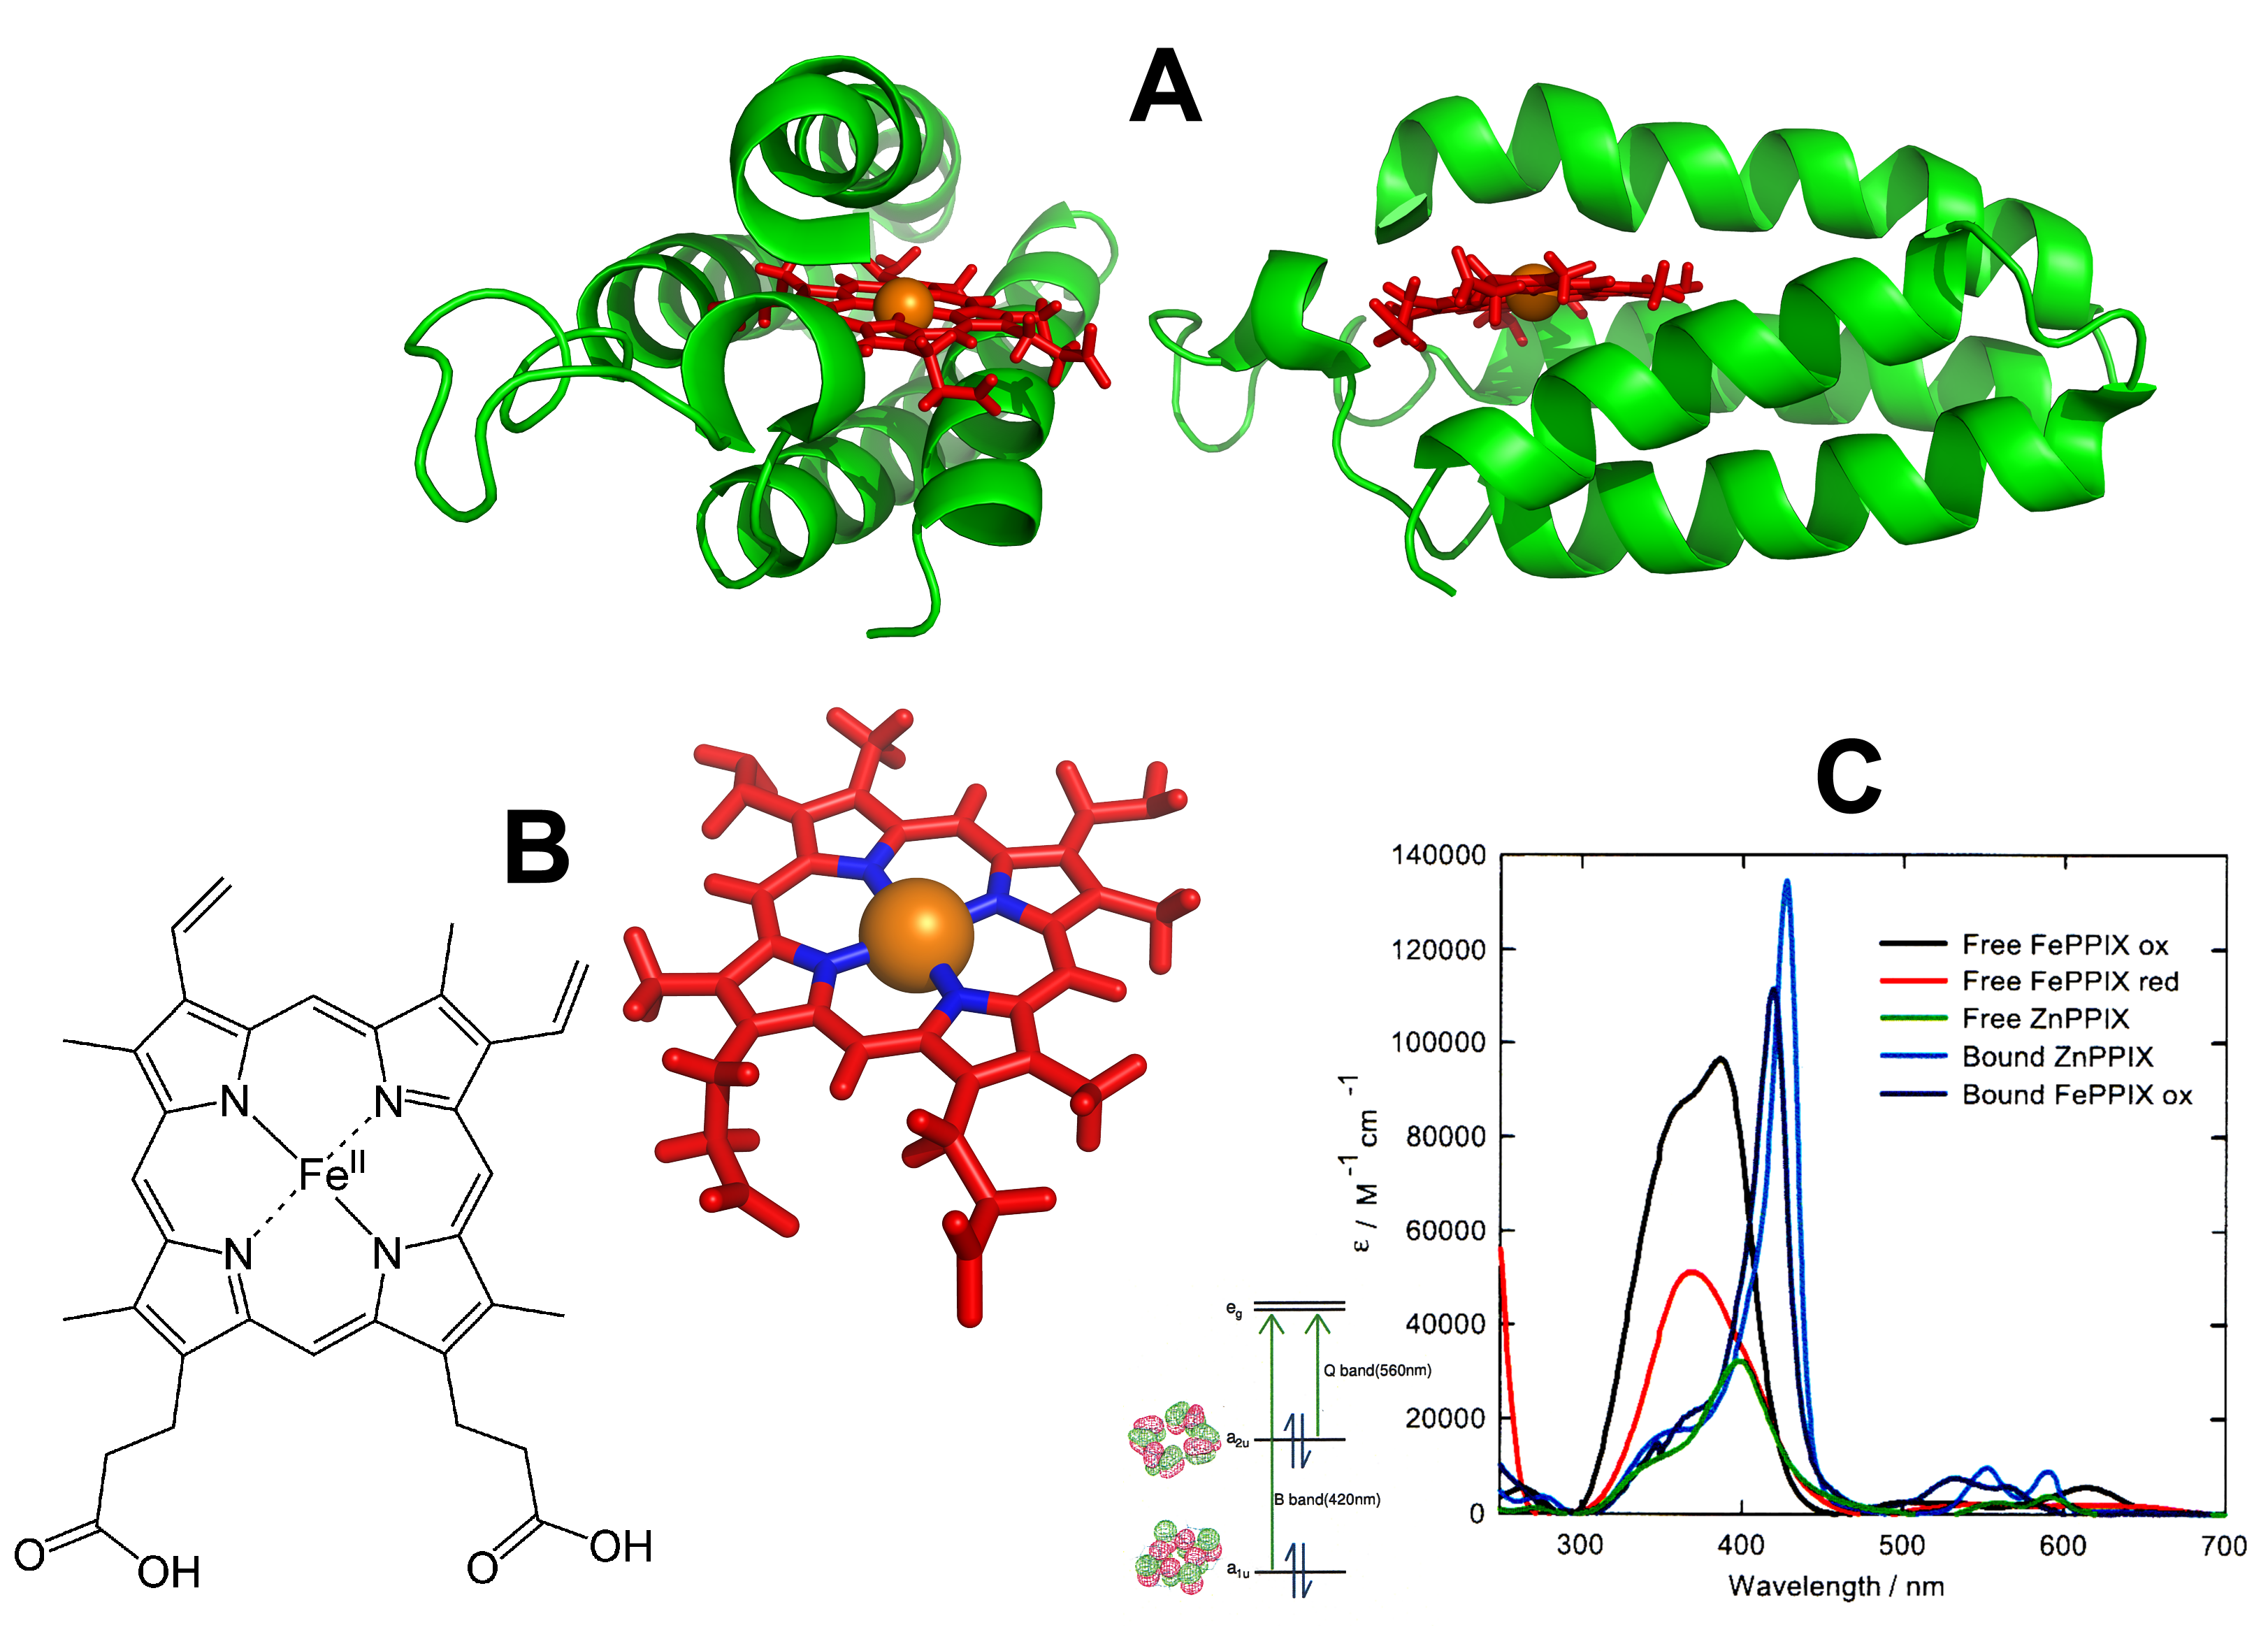
\includegraphics[width=137.4mm]{Images/haemStructure.png}
	\caption[Haem Structure]{A fancy image.}
	\label{fig:haemStructure}
\end{figure}
\end{verbatim}

\vspace{2ex}

\begin{figure}[!th]
	\centering
	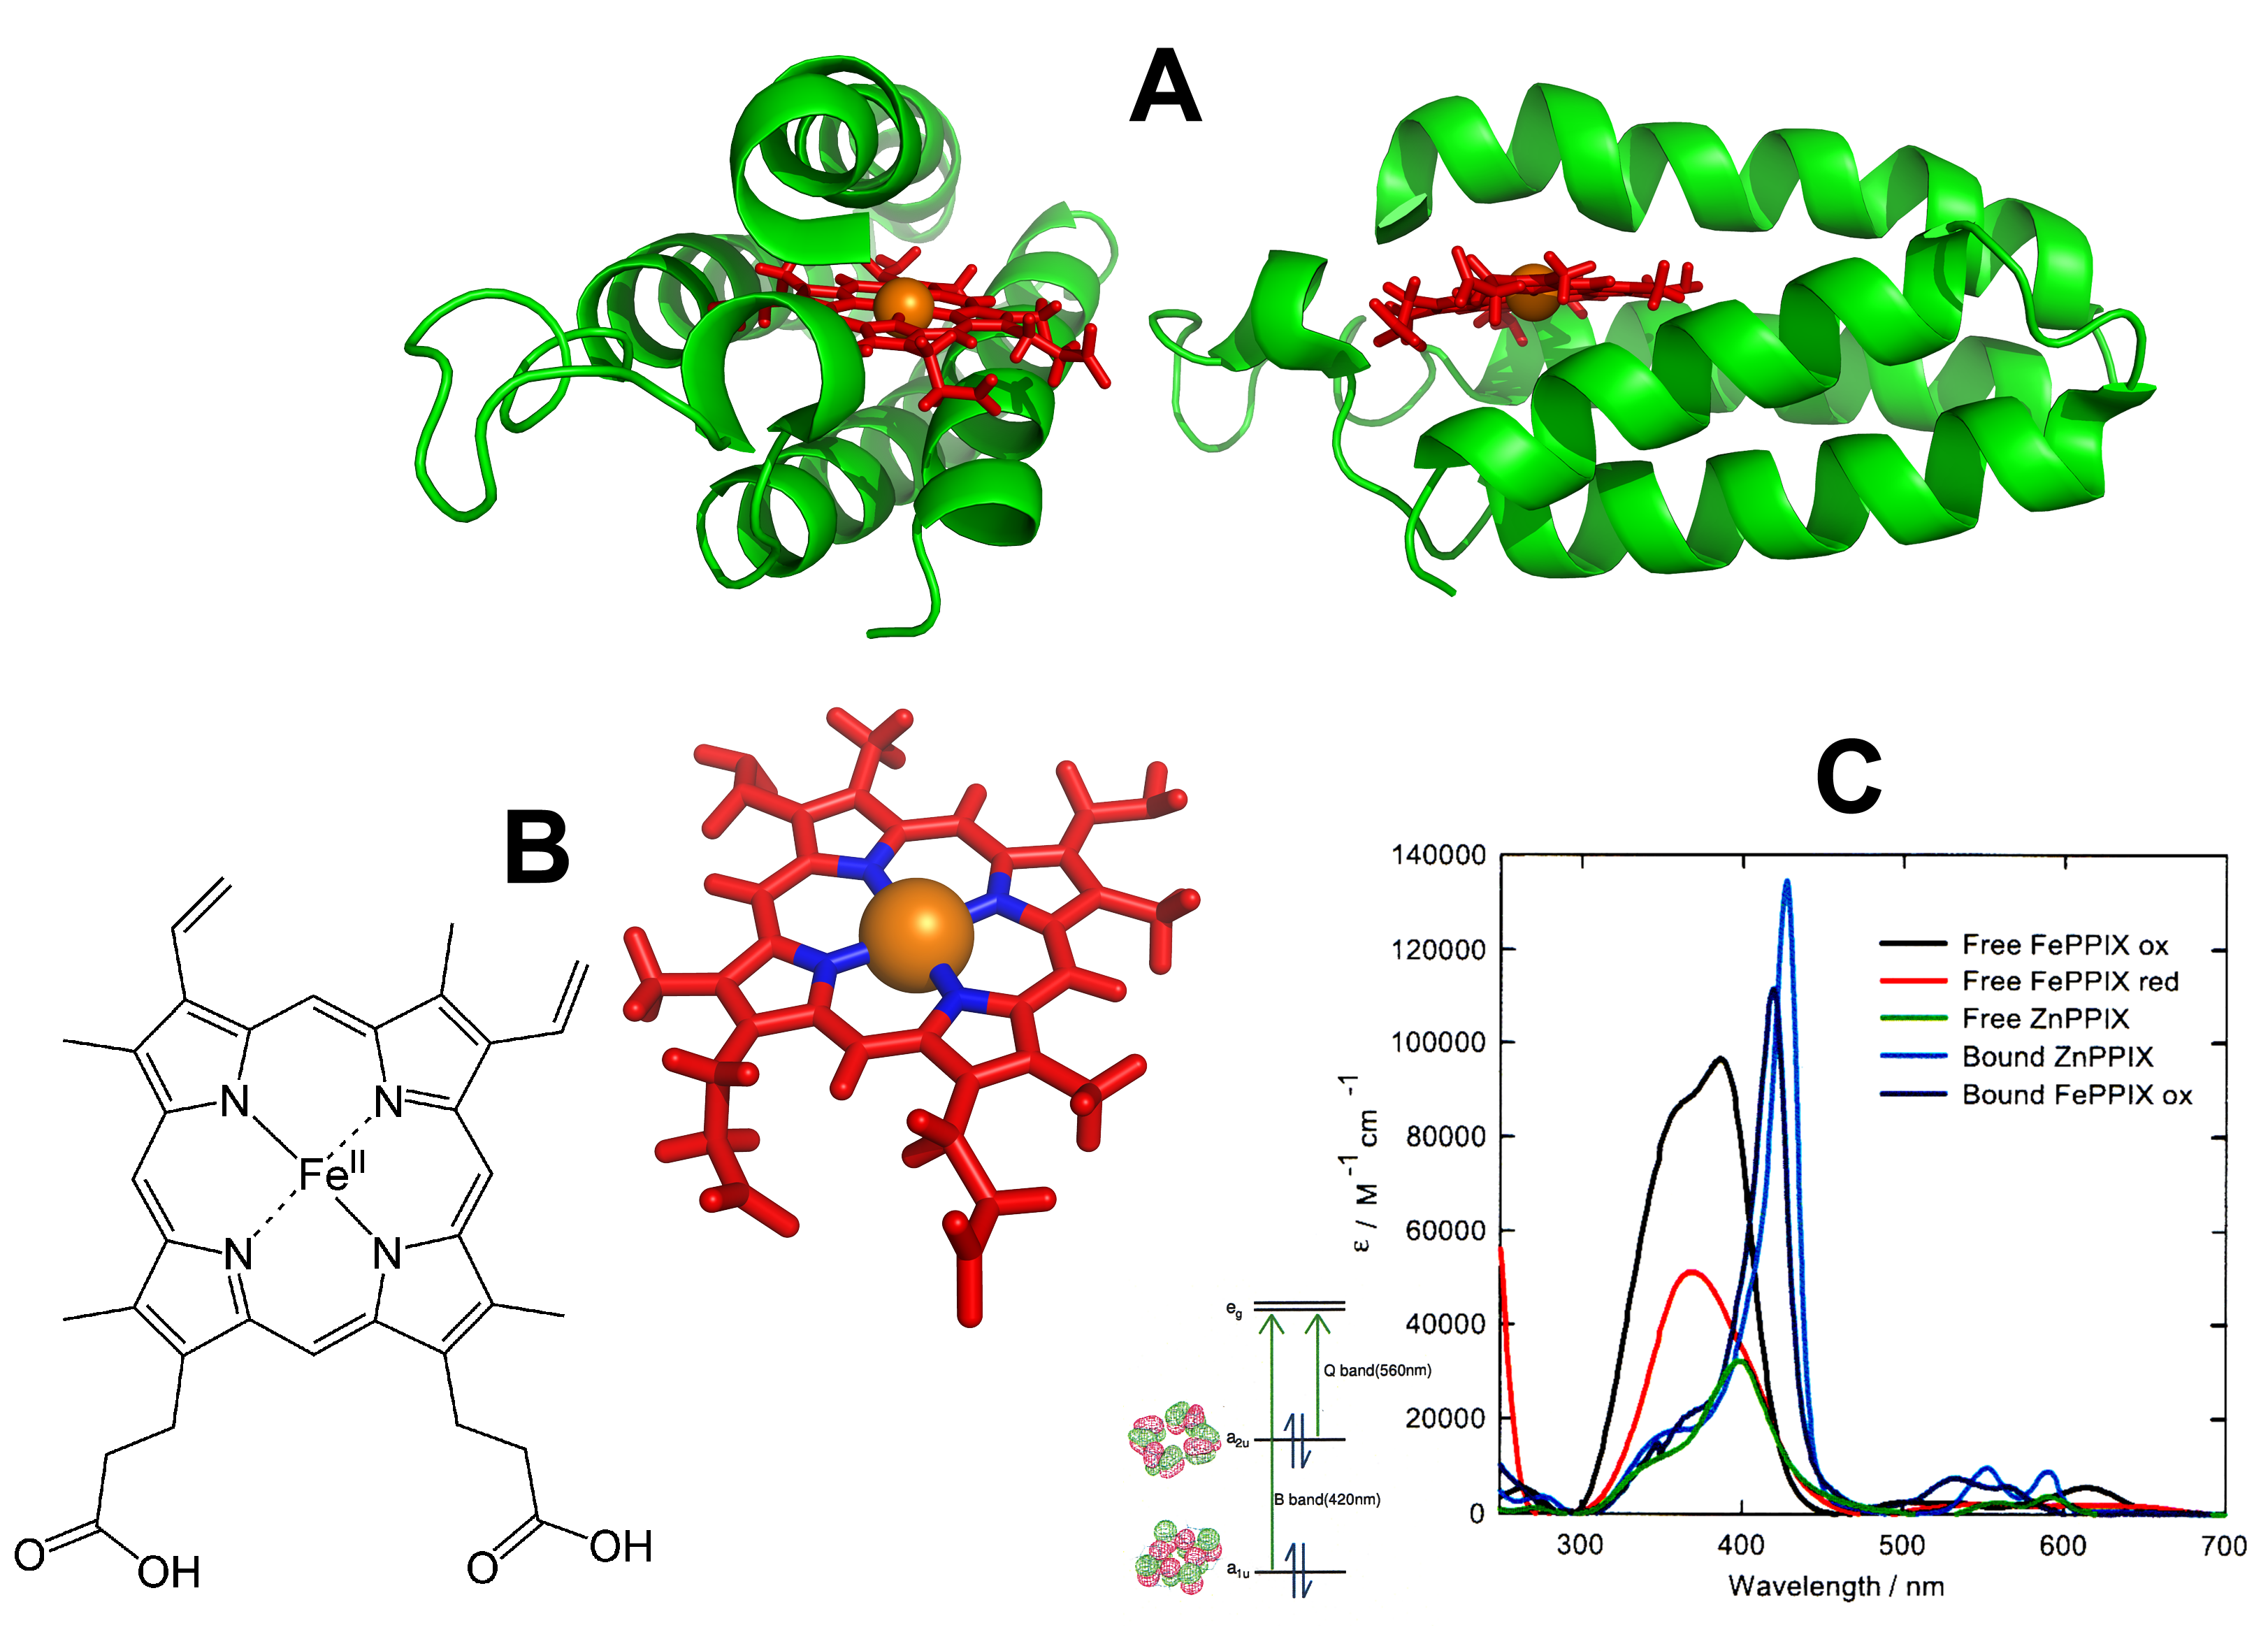
\includegraphics[width=137.4mm]{Images/haemStructure.png}
	\caption[Haem Structure]{A fancy image from Chris' Thesis.}
	\label{fig:haemStructure}
\end{figure}

In this example the command {\textbackslash}includegraphics tells LaTeX to look in the directory `Images' and incorporate the file called `haemStructure.png' into the final document while setting the width to 137.4mm.  This command can be used to resize a graphical file using the height or width parameter as shown. You must specify the units which can be pt, ex, em, mm, cm and so on. LaTeX recognises a very wide variety of standard units and graphics formats. The command is part of the graphicx package and so in the preamble you must include the command {\textbackslash}usepackage\{graphicx\}.

Many packages have been written to provide new commands. For example the `subfigure' package enables you to place separate images or files in the same figure side by side while giving them their own label. However, in this document we only concentrate on the very basics.

\section{Floating Environments}

Both tables and figures are examples of a `floating environments' which means LaTeX decides where to put them. 

The mysterious [!tbh] letters give guidance to LaTeX about roughly where the figure or table is  allowed to be, but in general they can move a long way from where you position them within your text file.  The letters in the square bracket can be t, h or b which stand for top, here or bottom.  If you don't specify any letters LaTeX defaults to [t].

LaTeX will always preserve the order in which figures appear.  If it cannot find a type setting solution, then it may move the float to it's own page, and combine it with other figures. If it still can't fit that in for some reason then it moves the float to the end of the document.  This has the effect of pushing all the remaining floating environments to the end of the document also.

The exclamation mark instructs LaTeX to ``try harder'' at putting the float where you told it to. Often you must play around to ensure the float positioning is acceptable, but usually this can be achieved by stretching or shrinking the image slightly using the size parameter, re-ordering text, judicial applications of the {\textbackslash}pagebreak command or by shouting loudly and slapping the computer monitor about. Note that it is better to resize the image using the original program that was used to create the image. Also using vector graphics can assist be useful (e.g. eps files) because they are designed to scale better.
\chapter{The Chapter on Making Chapters}
\label{sec:Chapters}

Right. LaTeX forces you to structure your document. There a series of simple commands for achieving this:

\vspace*{2ex}

{\textbackslash}chapter\{chapterName\}

{\textbackslash}section\{sectionName\}

{\textbackslash}subsection\{subsectionName\}

{\textbackslash}subsubsection\{subsubsectionName\}

\vspace*{2ex}

Easy enough. At the start of each chapter or section just issue one of these commands to name the section and LaTeX will present the chapter heading in the right style of font, which will be the same style of all the other heading names at that level of hierarchy throughout the document. In addition LaTeX assigns a number to that section. For example, this chapter was created using the command:

\vspace*{2ex}

{\textbackslash}chapter\{The Chapter on Making Chapters\} 

\vspace*{2ex}

LaTeX assigns the correct chapter number to each chapter in turn and then puts it in the table of contents, as you can see by looking at the table of contents! Easy.

\pagebreak
\section{The Section About Sections}
\label{sec:Section}
I think you're getting the hang of this. This section was created using the command {\textbackslash}section\{The Section About Sections\}. It appears in the table of contents as section \ref{sec:Section}.

\subsection{The Sub-Section About Sub-Sections}
\label{sec:SubSection}
Now you're really getting the hang of this. This subsection was created using the command {\textbackslash}subsection\{The Sub-Section About Sub-Sections\}. 

\subsubsection{The Sub-Sub-Section About Sub-Sub-Sections}
\label{sec:SubSubSection}
Now you're really getting the hang of this. but.. caught you out! This subsubsection doesn't have a number!  Ha Ha! It was created using the command {\textbackslash}subsubsection\{The Sub-Sub-Section About Sub-Sub-Sections\} in the same vein as all the other subsections/chapters etc. Here we have stopped the depth of the section numbering at the second level with the command:

\vspace*{2ex}

{\textbackslash}setcounter\{secnumdepth\}\{2\}

\vspace*{2ex}

Easy. WYSIWYM.  LaTeX does what you tell it to do. This is both a blessing and a curse.

\pagebreak
\section*{The Section About Sections That Don't Appear in the Table of Contents}
\label{sec:InvisibleSection}
Ok. Now we're throwing a spanner in the works. This section was created using the command:

\vspace*{2ex}

{\textbackslash}section*\{The Section About Sections That Don't Appear in the Table of Contents\}. 

\vspace*{2ex}

Notice how LaTeX has not assigned a number to the section and it doesn't appear in the table of contents. The effect of the * is to suppress the inclusion of a chapter, section or subsection in the automatic numbering. Easy. You can do this at any level. This is useful for things like prefaces, tables of contents or acknowledgements which you may or may not wish to have an entry in the main contents table. Up to you. It's your thesis. Don't just copy me.

\section{A Small Point About Numbering}

In this section notice how the numbering starts from where it left off before we suppressed the numbering on the previous section. Easy. WYSIWYM.
\pagebreak
\section{The Section About Internal Referencing}
\label{sec:InternalReferencing}

There are two related commands:

\vspace*{2ex}

{\textbackslash}label\{labelName\} 

{\textbackslash}ref\{labelName\}

\vspace*{2ex}


The {\textbackslash}label\{\} command allows you to create a label in a particular environment\footnote{That's right. Chapters, Sections and sub-sections etc are environments!}. The label won't appear in the final document. It's just a label which makes it easy to refer back to any particular environment elsewhere in the document. The {\textbackslash}ref\{\} command enables you to insert a reference anywhere in the document to any label in the document.  For example this is section \ref{sec:InternalReferencing}. The names you use in a label can be anything you like but musn't contain whitespace or special characters. I used the two commands:

\vspace*{2ex}

{\textbackslash}label\{sec:InternalReferencing\}

{\textbackslash}ref\{sec:InternalReferencing\}.

\vspace*{2ex}

The astute among you will realise that LaTeX has to read the document several times. Once to find the labels and then again to populate the references with the correct numbers. So you have to compile a latex document twice to get the referencing right. If there is a missing label or you refer to something that doesn't exist then latex inserts a convenient ? at that point. So hunting for queries is useful way of finding broken references. Latex issues warnings when it finds broken references.

As you create a document you will find yourself putting labels in all over the place so choose a sensible naming convention to help you remember the label names.

Each type of environment (equations, figures, tables, sections etc) has its own independent numbering system.  So when you choose your label name it's a good idea to have an identifier for that type of environment.  I have my own convention for label names which I use to help me remember references. E.g.   sec:SectionAboutCats. Eqn:EquationAboutCats,  Fig:FigureAboutCats and so on. This means you can differentiate between referring to the section or the figure more easily, even though they are about the same thing.

So Internal Referencing is a doddle. Easy!
\chapter{External Referencing}

Referencing is usually performed using a separate program called BibTex.  This program understands the file format .bib.

To create a reference within your document first you must create a .bib file by exporting your list of references from which ever referencing software you used, such as endnote, mendeley or whatever you use.

You can refer to an entry in the .bib file using the {\textbackslash}cite\{ref:Name\} command. the identifier `ref:Name' is the unique identifier which is the first line of each item included in your bibliography file.

For example, open the file LaTexCourseBib.bib in the bibliography directory. The first entry has the identifier `Horcas2007'.  This can be invoked as follows:


\begin{verbatim}
For example, this interesting fact\cite{Horcas2007}, is a cracking example.
\end{verbatim}

For example, this interesting fact\cite{Horcas2007}, is a cracking example.

During compilation latex and bibtex co-operate. During the first compilation latex generates a list of references that it needs.  During the second compilation bibtex populates the details from the .bib file into a shorter, ordered .bib file. The third compilation inserts markers at the right place in the main file and the fourth compilation generates the final list of references. Thus the compilation sequence is latex, bibtex, latex, latex.

The style of the referencing format can be changed using the command {\textbackslash}bibliographyStyle\{\}. e.g. the style used in this document is cjfthesisv1.bst which is invoked by 

\begin{verbatim}
\bibliographystyle{Bibliography/cjfthesisv1}
\end{verbatim}

The location of the list of references in the document is specified by issuing the {\textbackslash}bibliography\{\} command which also specifies the master bibliography file.

\begin{verbatim}
\bibliography{Bibliography/LaTeXCourseBib}
\end{verbatim}




\chapter{Organising Your Files}
One of the drawbacks of word is that the figures and tables are included within the document which becomes very very clunky quite quickly and once it reaches around 100Mb it becomes unwieldy and hard to export. One of that advantages of LaTeX is that the files are all text files and so are very light on resources and are easy to email around the place.

However, sometimes it can be difficult to navigate through a single text file, so if you had a huge document then it becomes difficult to find your way around.  One way of circumnavigating this problem is to break the file up into smaller files. As long as LaTeX knows where to look you can have a file for each logical sub-division of your document.

Therefore it is worth spending a bit of time at the beginning of a large project deciding how you wish to break up your LaTex Files and organise them neatly and tidily.  You can then tell LaTex where to look for the files using the following command:

\vspace*{2ex}
{\textbackslash}include\{fileName\}
\vspace*{2ex}

\pagebreak
\section{Linking a File}
We are now going to copy part of the tutorial file into a separate files and link it the main file.  Because this could go wrong it is sensible to back up tutorial.tex as something else. So save a copy called `tutorialOriginal.tex' for safe keeping. Then follow the following instructions.

\begin{enumerate}
\item Create a new file called MyFirstPage.tex
\item Select and Cut out the first chapter of Tutorial.Tex
\item Paste the first chapter into MyFirstPage.tex
\item Save both tutorial.tex and MyFirstPage.tex
\item Then add {\textbackslash}include\{MyFirstPage\} in tutorial.tex where the text used to be before you cut it out. We don't need to add the `.tex' because LaTeX can only include `.tex' files.
\item compile tutorial.tex and view the PDF
\end{enumerate}

The final PDF should look exactly the same as it was! except we now have a separate file for one of the chapters.

\pagebreak
\section{Creating A Class File}
We can also save our preamble in a separate file called a class file. This makes your main document much easier to understand.  To make it work we need to use the {\textbackslash}LoadClass\{\} command as follows: 

\begin{enumerate}
\item Create another new file and save it as TutorialStyle.cls
\item Copy the preamble of tutorial.tex into the new file. Starting with the {\textbackslash}documentclass{} command and copy right up to, but not including, the {\textbackslash}begin{document} command. Delete the preamble in the original document.
\item Save TutorialStyle.cls and tutorial.tex
\item Modify the first line of TutorialStyle.cls by replacing the word `document' with the word `Load'.
\item Add a new first line of tutorial.tex to use your new style class {\textbackslash}documentclass\{TutorialStyle\}
\item Save both files.
\end{enumerate}

\subsection{Sanity Check}

The first line of TutorialStyle.cls should now be:

\begin{verbatim}
\LoadClass[12pt, oneside, a4paper]{book}
\end{verbatim}
\vspace{2ex}

The first line of tutorial.tex should be:

\begin{verbatim}
\documentClass{TutorialStyle}
\end{verbatim}
\vspace{2ex}

We have just created what is called a style file. You can use this style file as a generic preamble for other documents as well. Compile tutorial.tex.  Nothing should have changed in the final PDF.


\pagebreak
\section{The Structure of this Document}

Lets now look at how I've organised this document. It is identical to my thesis because it started out life as my thesis. I usurped the structure and simply replaced the headings and content to make a kind of reference manual for this introductory course. This document therefore is three things:

\begin{enumerate}
\item An example thesis structure to work from.
\item The LaTeX files which were used to create it can be used as a template for a thesis.
\item It is also a convenient introductory latex manual!
\end{enumerate}

\vspace*{2ex}
Groovy huh?

\section{The Master File}

There is a master file where LaTeX begins the compilation procedure. This contains the {\textbackslash}documentclass command needed to set the ball rolling. Within the file there are a series of {\textbackslash}include\{\} commands, one for each Chapter, which tell LaTeX where to find the files containing each chapter.

The subfiles cannot be compiled on their own because they do not contain the {\textbackslash}documentclass, {\textbackslash}begin\{document\} or {\textbackslash}end\{document\} commands. Lets us look in more detail at the master file and we will learn some new LaTeX commands.

\singlespacing
\pagebreak
\begin{verbatim}
\documentclass{Style/LatexCourseStyle}

\begin{document}
\setcounter{secnumdepth}{2}
\setcounter{tocdepth}{1}

\frontmatter
\onehalfspacing
\include{Frontmatter/Titlepage}
\include{Frontmatter/Declaration}
\include{Frontmatter/Acknowledgements}
\include{Frontmatter/Summary}
\include{Frontmatter/Abbreviations}
\tableofcontents
\listoftables
\listoffigures

\mainmatter
\renewcommand{\sectionmark}[1]{\markright{\thesection \ #1}{}}
\include{Chapters/Overview}
\include{Chapters/MyFirstPage}
\include{Chapters/Lists}
\include{Chapters/mathsEquations}
\include{Chapters/ChemicalEquations}
\include{Chapters/Tables}
\include{Chapters/Figures}
\include{Chapters/Sectioning}
\include{Chapters/externalReferencing}
\include{Chapters/ThesisTemplateMainFile}
%\include{Chapters/ChapterThatIsNotCompiled}

\appendix
%\include{Appendices/UsefulWebsites}

\singlespacing

\backmatter
\addcontentsline{toc}{chapter}{References}
\bibliographystyle{Bibliography/cjfthesisv1}
\renewcommand{\bibname}{References}
\bibliography{Bibliography/LatexCourseBib}

\end{document}
\end{verbatim}
\onehalfspacing
\pagebreak

\section{Analysing the Master File}
Let us go through this file and observe the new commands. Most of it is self-explanatory.

\begin{verbatim}
\documentclass{Style/LaTeXCourseStyle}
\end{verbatim}

This command tells latex that the document class is the one defined in the the style file ''LaTeXCourseStyle'', which is in the sub directory ''style''.  Easy.

\begin{verbatim}
\setcounter{secnumdepth}{2}
\setcounter{tocdepth}{1}
\end{verbatim}

The first of these commands tells latex that the section depth number is 2. I.E. throughout the document only bother numbering sections, subsections and subsubsections down to the second level (such as section 1.2.3). The second command tells latex to only build the table of contents from section numbers down to the first level i.e. 1.1.  Easy enough.

The command {\textbackslash}frontmatter is exclusive to the book class, on which this style is based, and tells latex that within this section to number the pages using roman numerals, and not to include these numbers in the table of contents, just like in a book. The {\textbackslash}mainmatter and {\textbackslash}backmatter commands similarly delineate the other sections of the document.  

Childs play.  How long would it take you to figure out how to do that in word???? No idea. I've never tried.

Note that these rather cool commands are not available in every single class. So for a paper you would use the article class where such compartmentalisation of your document is not appropriate. In fact you can often download latex templates from the journal to wish to submit your paper, which is why I concentrate on the thesis template in this course.

\begin{verbatim}
\onehalfspacing
\end{verbatim}

Is obvious. ''From this point forward use line spacing of one and a half lines please. Thank you.'' How many hours have you spent clicking on paragraph indentations for each separate paragraphs in word? Nightmare. Want to change the standard in the whole document? Not a chance in word. In latex, you can do it with a single word, carefully placed in the master file.

\begin{verbatim}
\include{Frontmatter/Titlepage}
\include{Frontmatter/Declaration}
\include{Frontmatter/Acknowledgements}
\include{Frontmatter/Summary}
\include{Frontmatter/Abbreviations}
\end{verbatim}

The {\textbackslash}include\{\} command tells latex to include the specified .tex file at this point.  Thus it is a simple matter to break up a large document into sub components.  I have written each part of the front matter in a separate file and then grouped all the front matter into one directory called: Frontmatter.

See how the directory structure of my files reflects the structure of my book?

\begin{verbatim}
\tableofcontents
\listoftables
\listoffigures
\end{verbatim}

Again. This is easy. These commands mean: ''Please scan through the whole document and build for me a table of contents, a list of tables, a list of figures and then write down the entries along side their section numbers (as I have them ordered in this version of the document), as well as the page numbers on which they appear and create a nice little summary table and add them to the front matter of my document. Thanks.''.

How does latex do this?  remember the idea of environments?  Well each table, figure, equation etc is a defined environment.  LaTeX just counts them up and assigns numbers starting wherever you want and builds a table.  You can tell latex to ignore individual sections if you want to.

You can also control the look and feel of your table of contents with subtley and grace. Do you want to fill the white space with lines of dots to aid readability, even though the chapter titles are all different lengths? page numbers? How deep should the TOC been?  etc etc etc. How to do this is beyond the scope of this course, but now you know about it, go look it up. easy as $\pi$.

Ok.

Main matter we've done.

\begin{verbatim}
\renewcommand{\sectionmark}[1]{\markright{\thesection \ #1}{}}
\end{verbatim}

This command tells latex to 'renewcommand', i.e. change the meaning of the following command from this point in the document forward, over-riding previous definitions.
\begin{verbatim}
\sectionmark}[1]{\markright{\thesection \ #1}{}
\end{verbatim}

Is latex speak for ``please write the section heading at the top right hand side of each page. thanks''. This works in conjunction with a command in the style file which we'll talk about later. You have to tell latex to switch on headings as well as where to put them.

\begin{verbatim}
\include{Chapters/Overview}
\include{Chapters/MyFirstPage}
\include{Chapters/Lists}
\include{Chapters/mathsEquations}
\include{Chapters/ChemicalEquations}
\include{Chapters/Tables}
\include{Chapters/Figures}
\include{Chapters/Sectioning}
\include{Chapters/externalReferencing}
\include{Chapters/ThesisTemplateMainFile}
%\include{Chapters/ChapterThatIsNotCompiled}
\end{verbatim}

This is the include command again. You will notice that one of the include lines is commented out. This is a handy trick to only build certain parts of my thesis. Which can be useful if individual chapters are being reviewed.

\pagebreak

\begin{verbatim}
\appendix
%\include{Appendices/UsefulWebsites}

\singlespacing

\backmatter
\addcontentsline{toc}{chapter}{References}
\bibliographystyle{Bibliography/cjfthesisv1}
\renewcommand{\bibname}{References}
\bibliography{Bibliography/LatexCourseBib}
\end{verbatim}

The rest is easy. {\textbackslash}Appendix means we are in the appendix now and start labelling sections with A.1.2 instead of 1.2.3.  

{\textbackslash}addcontentsline means forcibly insert a contents line about the references into the contents table. 

{\textbackslash}\{bibliographystyle\{Bibliography/cjfthesisv1\}\} means use the biblography style defined in the file cjfthesisv1. Defining a bibliography style will be covered later if we have time. This is where you specify how the references will appear (names, journals, full stops, commas etc).

{\textbackslash}renewcommand\{{\textbackslash}bibname\}\{References\} means: rename the bibliography chapter as `References'

{\textbackslash}biblography means add the following bibliography.  You can reference entries in this bibliography file very easily.

The astute among you will realise that LaTeX will have to read the document several times before it can be compiled with all the references.  Hey ho. No problem. You can go and have a cuppa while LaTeX does your references for you in the style of your favorite journal... nice.




%\include{Chapters/ChapterThatIsNotCompiled}
\end{verbatim}

This is the include command again. You will notice that one of the include lines is commented out. This is a handy trick to only build certain parts of my thesis. Which can be useful if individual chapters are being reviewed.

\pagebreak

\begin{verbatim}
\appendix
%\include{Appendices/UsefulWebsites}

\singlespacing

\backmatter
\addcontentsline{toc}{chapter}{References}
\bibliographystyle{Bibliography/cjfthesisv1}
\renewcommand{\bibname}{References}
\bibliography{Bibliography/LatexCourseBib}
\end{verbatim}

The rest is easy. {\textbackslash}Appendix means we are in the appendix now and start labelling sections with A.1.2 instead of 1.2.3.  

{\textbackslash}addcontentsline means forcibly insert a contents line about the references into the contents table. 

{\textbackslash}\{bibliographystyle\{Bibliography/cjfthesisv1\}\} means use the biblography style defined in the file cjfthesisv1. Defining a bibliography style will be covered later if we have time. This is where you specify how the references will appear (names, journals, full stops, commas etc).

{\textbackslash}renewcommand\{{\textbackslash}bibname\}\{References\} means: rename the bibliography chapter as `References'

{\textbackslash}biblography means add the following bibliography.  You can reference entries in this bibliography file very easily.

The astute among you will realise that LaTeX will have to read the document several times before it can be compiled with all the references.  Hey ho. No problem. You can go and have a cuppa while LaTeX does your references for you in the style of your favorite journal... nice.




%\include{Chapters/ChapterThatIsNotCompiled}

\appendix
%\include{Appendices/UsefulWebsites}

\singlespacing

\backmatter
\addcontentsline{toc}{chapter}{References}
\bibliographystyle{Bibliography/cjfthesisv1}
\renewcommand{\bibname}{References}
\bibliography{Bibliography/LatexCourseBib}

\end{document}
\end{verbatim}
\onehalfspacing
\pagebreak

\section{Analysing the Master File}
Let us go through this file and observe the new commands. Most of it is self-explanatory.

\begin{verbatim}
\documentclass{Style/LaTeXCourseStyle}
\end{verbatim}

This command tells latex that the document class is the one defined in the the style file ''LaTeXCourseStyle'', which is in the sub directory ''style''.  Easy.

\begin{verbatim}
\setcounter{secnumdepth}{2}
\setcounter{tocdepth}{1}
\end{verbatim}

The first of these commands tells latex that the section depth number is 2. I.E. throughout the document only bother numbering sections, subsections and subsubsections down to the second level (such as section 1.2.3). The second command tells latex to only build the table of contents from section numbers down to the first level i.e. 1.1.  Easy enough.

The command {\textbackslash}frontmatter is exclusive to the book class, on which this style is based, and tells latex that within this section to number the pages using roman numerals, and not to include these numbers in the table of contents, just like in a book. The {\textbackslash}mainmatter and {\textbackslash}backmatter commands similarly delineate the other sections of the document.  

Childs play.  How long would it take you to figure out how to do that in word???? No idea. I've never tried.

Note that these rather cool commands are not available in every single class. So for a paper you would use the article class where such compartmentalisation of your document is not appropriate. In fact you can often download latex templates from the journal to wish to submit your paper, which is why I concentrate on the thesis template in this course.

\begin{verbatim}
\onehalfspacing
\end{verbatim}

Is obvious. ''From this point forward use line spacing of one and a half lines please. Thank you.'' How many hours have you spent clicking on paragraph indentations for each separate paragraphs in word? Nightmare. Want to change the standard in the whole document? Not a chance in word. In latex, you can do it with a single word, carefully placed in the master file.

\begin{verbatim}
\thispagestyle{empty}

\begin{center}
\vspace*{\stretch{1}}

\hrule height 2pt
\vspace*{2ex}
{\Huge\textbf{Towards the Ability to Make Super Duper LaTeX Documents}\par}
\vspace*{2ex}
\hrule height 2pt
\vspace*{10ex}
{
\includegraphics[height=40mm]{Images/UnivShield}\par}
\vspace*{10ex}
{\large\textbf{Christopher~James~Forman}\par}
\vspace*{2ex}
{\large{Department Of Chemistry}\par}
\vspace*{2ex}
{\large{University of Cambridge}\par}
\vspace*{5ex}
{\large{This dissertation is submitted for the degree of \textit{Doctor of Philosophy}}\par}
\vspace*{5ex}
{\large{\today}\par}

\vspace*{\stretch{2}}
\end{center}
\chapter*{Declaration}

\vfill

This dissertation is the result of my own work and includes nothing which is the outcome of work done in collaboration except where specifically indicated in the text. It is not substantially the same as any that I have submitted for a degree or diploma or other qualification at any other University and no part has already been, or is concurrently being, submitted for any degree, diploma, or other qualification. It does not exceed 60,000 words, including tables, footnotes, bibliography and appendices.\par

\vspace{10ex}

\begin{flushright}
Signature: \rule[0pt]{60mm}{0.5pt}

\vspace{5ex}

Date: \rule[0pt]{60mm}{0.5pt}
\end{flushright}

\vfill
\chapter*{Acknowledgments}
\subsection*{Family}
Mum. Dad. Pet Dog.

\subsection*{Scientific Collaborations}
Dr A.N.Other at uni of blah for samples and instrument time etc. My Amazing Lab Chums.

\subsection*{Scientific Support}
My amazing lab chums.

\subsection*{General Assistance}
Cleaner, My amazing lab chums.

\subsection*{Financial Support}
Bank, Tax payer. My amazing lab chums.

\subsection*{Moral Support}
My Amazing Lab chums.

\subsection*{Academic Inspiration}
Netwon, My super. My Amazing Lab Chums.

\subsection*{Everyone else}
My Amazing Lab Chums.

\chapter*{Summary}
This document is a handbook for introducing you to LaTeX. It contains a bit of background about the history and philosophy of LaTeX.  However, it concentrates on providing a guided practical introduction to the basic techniques such as 
\begin{itemize}
\item Lists
\item Mathematical and chemical equations
\item Tables
\item Figures
\item Chapters and Sections
\item Linking to other files in large documents
\item Referencing
\end{itemize}

The handbook is also presented in the style of a thesis. This means that source files provided on the introductory course and available from the department web page are a convenient template for a thesis.

More details on specific aspects of LaTeX can be found at the departmental LaTeX page which can be found here:

 http://www-ch-int.ch.private.cam.ac.uk/latex/about

\chapter*{Abbreviations}

\begin{longtable}{r >{\rule{0pt}{3ex}}l<{\rule[-1.5ex]{0pt}{0pt}}}
ADP & Adenosine Diphosphate\\
(nc/c)AFM & (non-contact/conducting) Atomic Force Microscopy\\
ATP & Adenosine Triphosphate \\
\end{longtable}
\end{verbatim}

The {\textbackslash}include\{\} command tells latex to include the specified .tex file at this point.  Thus it is a simple matter to break up a large document into sub components.  I have written each part of the front matter in a separate file and then grouped all the front matter into one directory called: Frontmatter.

See how the directory structure of my files reflects the structure of my book?

\begin{verbatim}
\tableofcontents
\listoftables
\listoffigures
\end{verbatim}

Again. This is easy. These commands mean: ''Please scan through the whole document and build for me a table of contents, a list of tables, a list of figures and then write down the entries along side their section numbers (as I have them ordered in this version of the document), as well as the page numbers on which they appear and create a nice little summary table and add them to the front matter of my document. Thanks.''.

How does latex do this?  remember the idea of environments?  Well each table, figure, equation etc is a defined environment.  LaTeX just counts them up and assigns numbers starting wherever you want and builds a table.  You can tell latex to ignore individual sections if you want to.

You can also control the look and feel of your table of contents with subtley and grace. Do you want to fill the white space with lines of dots to aid readability, even though the chapter titles are all different lengths? page numbers? How deep should the TOC been?  etc etc etc. How to do this is beyond the scope of this course, but now you know about it, go look it up. easy as $\pi$.

Ok.

Main matter we've done.

\begin{verbatim}
\renewcommand{\sectionmark}[1]{\markright{\thesection \ #1}{}}
\end{verbatim}

This command tells latex to 'renewcommand', i.e. change the meaning of the following command from this point in the document forward, over-riding previous definitions.
\begin{verbatim}
\sectionmark}[1]{\markright{\thesection \ #1}{}
\end{verbatim}

Is latex speak for ``please write the section heading at the top right hand side of each page. thanks''. This works in conjunction with a command in the style file which we'll talk about later. You have to tell latex to switch on headings as well as where to put them.

\begin{verbatim}
\chapter{Overview}
\label{chap:overview}
\section{LaTeX: The answer to everything.}
LaTeX is typsetting program that takes an input file of marked up text and then, with a user defined set of rules, typesets a beautifully crafted output file that can be easily printed (e.g. a pdf). 

\subsection{Advantages}

The advantages of this method are manifold:

\begin{itemize}

\item Use any text editor to view the source document.
\item More time can be spent working on the content and not worrying about how text or figures interact in the layout until later on.
\item LaTeX uses consistent rules throughout a document
\item LaTeX sorts out basic typesetting automatically
\item Changes can be introduced globally with very little effort
\item Document structure is explicit
\item Documents can be professionally typeset and look great
\item You are forced to structure your documents correctly.
\item Mathematical equations, like $E=mc^2$ or $\imath\hbar\frac{\partial}{\partial t}\Phi (x, t) = \hat{H}\Phi (x, t)$ can be produced almost as fast as typing (if you know the commands!).
\end{itemize}

\subsection{Disadvantages}
The disadvanatges of this method are also manifold:
\begin{itemize}
\item You don't see the output as you go.
\item Steep learning curve.
\item Documents are harder to edit by a second author (unless they are adept at LaTeX too). This can be mitigated using version control, which makes group authoring processes superior to word.
\item The program never works quite the way you want it to and learning how to influence it can be problematic and subtle.
\item Although intended to save work the principle of 'conservation of work' means that you simply transform problems associated with WYSISYG approaches to problems associated with WYSIWYM approaches!
\item You can go blind trying to determine the difference between wiggly and smooth brackets if your editors font isn't large enough.
\end{itemize}

\subsection{On balance?}
If it's so rubbish, why use LaTeX?

\begin{itemize}
\item Large documents are much more easily handled. 
\item In general it is quicker to debug a LaTeX document than typeset an entire thesis manually. 
\item Technical information such as tables, equations and figures are integrated much more smoothly than with word.
\end{itemize}

\section{How does it work?}

The raw text is interspersed with commands, preceded by a \textbackslash, which tell LaTeX what to do with the text. For example you can \textbf{make it bold}, \emph{italic}, or \underline{underlined} with the commands {\textbackslash}textbf\{\}, {\textbackslash}emph\{\} or {\textbackslash}underlined\{\}. More on commands in a moment...



\chapter{My First Page}

\section{The Very Beginning}
The very simplest LaTeX document might look like this:

\begin{verbatim}
\documentclass[a4paper,12pt]{article}
\begin{document}
Hello World.
\end{document}
\end{verbatim}

\pagebreak
\thispagestyle{empty}
Hello World.
\pagebreak
\subsection{Break Down}
What's all the gobbledegook around my simple message???

In LaTeX we intersperse text and commands.  Commands are preceded by a \textbackslash. For example the first line in a LaTeX document \underline{\textbf{\emph{must}}} be:

\begin{verbatim}
\documentclass[options]{class}
\end{verbatim}

Where the word ''class'' may be substituted for one of many things such as: article, proc, minimal, report, book, letter, memoir, slides, beamer.

Similarly, and completely generally in LaTeX speak, the square brackets denote the existence of optional parameters. Each individual command can take its own parameters and for the ''{\textbackslash}documentclass'' command there are options for controlling font size, font family, landscape, oneside, twosided, page size and so on. These options will persist throughout the entire document. For example the document class command for this document, (which is likely to be like the one you would use for a thesis), would be:

\begin{verbatim}
\documentclass[12pt, oneside, a4paper]{book}
\end{verbatim}

Other options include:

\begin{itemize}
\item {10pt, 11pt, 12pt (default is 10pt).}
\item {letterpaper, legalpaper, a4paper, executivepaper, a5paper, b5paper}
\end{itemize}
and so on.

\pagebreak
\section{Can I start typing please?}

After we have set up the document we can start actual work on our document. So we must tell LaTeX that what follows is to be interpreted as a document.  The command {\textbackslash}begin can take many different parameters and is a command to enter what is known, in LaTeX speak, as 'an environment'. Thus the commands:
\begin{verbatim}
\begin{document}

\end{document}
\end{verbatim}

tells LaTeX to enter and leave the document environment, and thus constitute the outer limits of our document file. Other environments include the equation environment, the itemize environment, the figure environment and so on. These will be encountered in due course.

Every part of the LaTeX file is therefore within an environment of specific type and the content within each environment consists of commands or text.

That's basically it.

So let's get on with it shall we...

\pagebreak
\section{The ground rules}
\begin{quote}
Hold on, hold on, hold on my son.

First the lessons.

Then the fun!
\end{quote}
Dr Seuss.

\subsection{Spaces}
Whitespace characters, such as blank or tab, are treated uniformly as space by LaTeX. Several consecutive whitespace characters are treated as one single space. Whitespace at the start of a line is generally ignored, and a single line break is treated as whitespace. An empty line between two lines of text defines the end of a paragraph. Several empty lines are treated the same as one empty line. The text below is an example.

\begin{verbatim}
It does not matter whether you
enter one or several             spaces
after a word. The final result will be typeset beautifully
according    to     precise rules.




An empty line starts a new
paragraph. Note the indentation on the first line of the paragraph, 
except at the beginning of the section. 
\end{verbatim}

\vspace*{2ex}
\vspace*{2ex}

It does not matter whether you
enter one or several             spaces
after a word. The final result will be typeset beautifully
according    to     specific rules.




An empty line starts a new
paragraph. Note the indentation on the first line of the paragraph, except at the beginning of the section. 

\pagebreak
\subsection{Special Characters}
The symbols 

\# \$ \% \textasciicircum{} \& \_ \{ \} \~{} \textbackslash

are reserved characters that either have a special meaning under LaTeX or are unavailable in all the fonts. If you enter them directly in your text, they will normally not print, but rather make LaTeX do strange things.

To overide the special meanings of these symbols and allow them to produced within your text you may use the following sequences:
\begin{verbatim}
\# \$ \% \textasciicircum{} \& \_ \{ \} \~{} \textbackslash
\end{verbatim}

Other symbols and many more can be printed with special commands in mathematical formulae or as accents.

The backslash character '\textbackslash' cannot be entered by adding another backslash in front of it ( \textbackslash\textbackslash); because this sequence means ''linebreak''.

The command \textbackslash\~{}\{\} produces a tilde which is placed over the next letter. For example \textbackslash\~{}\{n\} gives \~{n}. To produce just the character \~{}, use \textbackslash\~{}\{\} which places a \~{} over an empty box.

Similarly, the command \textbackslash\textasciicircum{} produces a hat over the next character, for example \textbackslash\textasciicircum\{o\} produces \^{o}.

\pagebreak
\section{Preamble}
After the {\textbackslash}documentclass command we add ''preamble''. Here we load special features that we will use throughout our document to expand on the basic capabilities of LaTex. These are contained in units called ''packages'' which we can tell our LaTeX compiler to download by using the command ''{\textbackslash}include\{packageName\}''. 

There are many repositories of such packages on the web. Your compiler generally knows where to look and most standard packages are included with any install. For example, to include a special set of typesetting instructions to handle chemical equations we can grow our simple document with a single command like this:

\begin{verbatim}
\documentclass[a4paper,12pt]{article}
\usepackage[version=3]{mhchem}
\begin{document}
Hello World!

We all need \ce{H2O}.

I'm less fussed about \ce{^{235}_{92}U+}.

\end{document}
\end{verbatim}

\vspace{2ex}

\pagebreak
\thispagestyle{empty}
Hello World!

We all need \ce{H2O}.

I'm less fussed about \ce{^{235}_{92}U+}.
\pagebreak

Here we have loaded a package called: "`mhchem"' which took the option ''[version=3]''. This is a package for drawing chemical equations easily and it has it's own instruction manual which you can follow easily. It is included in the bundle of files for this course.

Other things we can do in the premable within LaTeX are to redefine existing commands or create our own personal commands. These can be stored in a file called the 'style file' which we can load at the beginning of our document, in place of our documentclass. More about this later on...


\subsection{Comments}
It is often useful to comment your LaTeX documents. You can leave yourself amusing, sarcastic messages that won't get printed out in the final document. Use this to make your own notes as the course progresses.

To get a comment use the \% command, which tells LaTeX to ignore the rest of the line, the line break and all the white space at the beginning of the next line, for example, we may add to our continually evolving document...

\begin{verbatim}
\documentclass[a4paper,12pt]{article}
\usepackage[version=3]{mhchem}
\begin{document}
Hello World!

%All humans need water and I would like 
%to include this concept in my arguments.
We all need \ce{H2O}.

%Uranium 235 is toxic, which is why I don't want to consume it... 
I'm less fussed about \ce{^{235}_{92}U+}.

\end{document}
\end{verbatim}

\vspace{4ex}
Hello World!

%All humans need water and I would like to include this concept in my arguments.
We all need \ce{H2O}.

%Uranium 235 is toxic, which is why I don't want to consume it... 
I'm less fussed about \ce{^{235}_{92}U+}.

\pagebreak
\section{Compiling}
Once the document is finished you can compile it. Your compiler will depend on the platform that you use. In the PWF we are using winEDT to edit the documents (a LaTeX front end) and texlive2008 which is the compiler itself. I use MiKTex and the front end texCenter.  There is no need to use a front end. If you prefer you can use a simple text editor and a command line.

the recommended distributions are:
\begin{itemize}
\item MiKTeX or TeX Live for Windows
\item TeX Live for Unix/Linux
\item MacTeX or TeX Live for Mac OS.
\end{itemize}

Once you have installed your software and got it working, written your source code and tried to compile it, there will nearly always be something wrong with your file. 

Any errors will be highlighted in the console window or error output box of your front end.  Some front ends dump the running commentary which LaTeX produces into a text file for easy reading afterwards.

In a compile attempt (successful or otherwise) LaTeX may produce the following files:

projectname.aux

projectname.bbl

projectname.lof

projectname.lot

projectname.txt

projectname.toc

projectname.dvi

These are interim files (toc= table of contents, bbl = bibliography etc). To be honest I have no idea what half of these things contain.  You only need the .tex file and a compiler with the right packages installed to produce them again.

Some versions of LaTeX only produce DVI files and you then need to convert the dvi file to a PDF or download a dvi viewer. You can also convert DVI files to PS files and then view them.  The good thing about front ends is that you can set them up to produce PDFs directly.

OK. So we have now produced a silly document but we understand it.  Now lets get on with learning how to make our own documents.



\chapter{Lists}
Lists are great.  The command {\textbackslash}begin\{\} can be used to enter a list environment.  For example:

\begin{verbatim}
\begin{itemize}
\item cat
\item dog
\item horse
\end{itemize}
\end{verbatim}

Produces:

\begin{itemize}
\item cat
\item dog
\item horse
\end{itemize}

\pagebreak
We can also replace the bullet points with numbers using the enumerate keyword.

\begin{verbatim}
\begin{enumerate}
\item cat
\item dog
\item horse
\end{enumerate}
\end{verbatim}

\begin{enumerate}
\item cat
\item dog
\item horse
\end{enumerate}

\pagebreak
and we can use the description keyword which does this:
\begin{verbatim}
\begin{description}
\item[Cat] a lovely furry creature with a cute nose and whiskers.
\item[Dog] Another furry creature that smells rather well; 
           its olfactory power stems from its nasal dampness.
\item [Horse] A large stinky creature with sideways facing eyes.
\end{description}
\end{verbatim}

\begin{description}
\item[Cat] a lovely furry creature with a cute nose and whiskers.
\item[Dog] Another furry creature that smells rather well; its olfactory power stems from its nasal dampness.
\item [Horse] A large stinky creature with sideways facing eyes.
\end{description}
\chapter{Maths Equations}

\section{Producing Beautiful Looking Mathematics}

One of the best features about LaTeX is `maths mode'.  For example the schrodinger equation can be produced as follows:

\vspace*{2ex}

\begin{center}
\begin{math}
\imath\hbar\frac{\partial}{\partial t}\Phi (x, t) = \hat{H}\Phi (x, t)
\end{math}
\end{center}

\vspace*{2ex}

\begin{verbatim}
\begin{math}
\imath\hbar\frac{\partial}{\partial t}\Phi(x,t)=\hat{H}\Phi(x,t)
\end{math}
\end{verbatim}

There are a number of ways to switch on maths mode.  The first, as above, is with the {\textbackslash}begin\{math\} environment. You can also enter mathmode inline using the \$ symbol. For example typing in \$y=ax\textasciicircum{}2+bx+c\$ yields $y=ax^2+bx+c$.  Another way is to enter the equation environment which enables you to number equations so you can then refer to them later in the text.

\begin{equation}
y(t)= \sin \left(\frac{{\alpha}t}{2\pi} + \phi_0\right)
\label{eqn:MadeUpNonsense}
\end{equation}

\vspace*{2ex}
\begin{verbatim}
\begin{equation}
y(t)= \sin \left(\frac{{\alpha}t}{2\pi} + \phi_0\right)
\end{equation}
\end{verbatim}.

\section{Basic Maths Mode}
Once in maths mode there is a kind of text based code for writing down your equations.  Here are the most basic symbols to get you going.
\begin{center}
\begin{tabular}{cc}
\toprule
Final Result & LaTeX Code \\
\cmidrule(){1-2}
$a+b$ & a+b \\
$a-b$ & a-b \\
$ab$ & ab \\
$a*b$ & a*b \\
$a \times b$ & a {\textbackslash}times b \\
$a \cdot b$ & a {\textbackslash}cdot b \\
$\frac{a}{b}$ & {\textbackslash}frac\{a\}\{b\} \\ 
$a^b$ & a\textasciicircum{}b \\
$a_b$ & a\_b \\
$\sin a$ & {\textbackslash}sin a  (same for cos, tan)\\
$ sin a$ & sin a \\
$\sqrt{a}$ & {\textbackslash}sqrt\{a\} \\
$\left( a \right) $ & {\textbackslash}left( a {\textbackslash}right)\\ 
$\left[ a \right]$ & {\textbackslash}left[ a {\textbackslash}right]\\ 
$\alpha$ & {\textbackslash}alpha \\
$\pi$ & {\textbackslash}pi \\
\bottomrule
\end{tabular}
\end{center}

A full treatise on maths mode is not practical here. There are lots of online tutorials and summaries of symbols. It just takes a bit of practice and you can build up equations really easily. It's straight forward to learn new stuff once you've done it a few times.

\pagebreak
\section{Equation Arrays}
Sometimes you need to arrange several equations vertically, referencing individual lines separately and aligning the equations on the $=$ sign. This can be achieved with equation arrays as follows:

\begin{eqnarray}
A\left( x\right) & = & \frac{x^2+2x+1}{x+1} \\
& = & \frac{\left(x+1\right)\left(x+1\right)}{x+1} \nonumber\\
& = & x+1 \nonumber\\
B(x,t) & = & \frac{e^{\left(\imath\omega_0 t + kx\right)}}{4\pi\epsilon_0}
\end{eqnarray}

\begin{verbatim}
\begin{eqnarray}
A\left( x\right) & = & \frac{x^2+2x+1}{1+x} \\
& = & \frac{\left(x+1\right)\left(x+1\right)}{1+x} \nonumber\\
& = & x+1 \nonumber\\
B(x,t) & = & \frac{e^{\left(\imath\omega_0 t + kx\right)}}{4\pi\epsilon_0}
\end{eqnarray}
\end{verbatim}

\begin{itemize}
\item Note the \& symbols. This tells LaTeX where to align the equations. There must be the same number of \& symbols in each line.
\item Note the \textbackslash\textbackslash ~at the end of each line except the last one. This symbol tells LaTeX to add another row in the array.  If you put it on the last line you get an empty row at the bottom of the array.
\item Note the {\textbackslash}nonumber command which suppresses line numbering for that line.
\item Note that equation number carries on from equation \ref{eqn:MadeUpNonsense} in the previous section.
\end{itemize}

\section{Maths Packages}

Maths mode comes as standard in LaTeX, however you can download packages that buff up your maths symbol set. For example neat vector notation comes in the package `vector'. e.g. {\textbackslash}uuvec\{T\} yields $\uuvec{T}$.

\begin{verbatim}
\usepackage{amssymb}
\usepackage{amsmath}
\usepackage{vector}
\end{verbatim}


\chapter{Chemical Equations}
The mhchem package means you can do basic stuff very easily using {\textbackslash}ce\{\}. For example:

\vspace{2ex}
\begin{verbatim}
\ce{CO2 + C -> 2CO}
\ce{CO2 + C <- 2CO}
\ce{CO2 + C <=> 2CO}
\ce{A-B=C#D\sbond E\dbond F\tbond G}
\end{verbatim}
\vspace{2ex}
\begin{center}
\ce{CO2 + C -> 2CO}

\ce{CO2 + C <- 2CO}

\ce{CO2 + C <=> 2CO}

\ce{A-B=C#D\sbond E\dbond F\tbond G}
\end{center}

\vspace{2ex}
You can also use math mode within chemical equations.
\vspace{2ex}

\begin{center}
\ce{$x\,$ Na(NH4)HPO4 ->[\Delta] (NaPO3)_{$x$} + $x\,$ NH3 ^ + $x\,$ H2O}
\end{center}

\begin{verbatim}
\ce{$x\,$ Na(NH4)HPO4 ->[\Delta](NaPO3)_{$x$} + $x\,$ NH3 ^ + $x\,$ H2O}
\end{verbatim}

And you can number chemical reactions as well by using the math mode equation environment.

\begin{equation}
\ce{CO2 + C <=> 2CO}
\end{equation}

\begin{verbatim}
\begin{equation}
\ce{CO2 + C <=> 2CO}
\end{equation}
\end{verbatim}

However, this will number mathematical and chemical equations using the same number system. There is a discussion in the mhchem pdf which shows you how to number chemical and mathematical equations independently. It's a bit complex and involves you creating your own type of environment... bit beyond the intro level of this course...
\chapter{Tables}
Tables are big business in Latex.  I use these packages to help me.

\begin{verbatim}
\usepackage{multirow}
\usepackage{booktabs}
\usepackage{dcolumn}
\end{verbatim}

Here's an example table

\begin{table}[!hb]
 \centering
	\begin{tabular}{@{}rccc@{~}r@{.}l*3{r@{.}l@{~}r@{.}l}D{.}{\cdot}{2,1}}
	\toprule
	\multicolumn{1}{c}{Fibre Type}
	& N 
	& M 
	&\multicolumn{3}{c}{$L_t$ (nm)}
	&\multicolumn{4}{c}{$R_t$ (nm)}
	&\multicolumn{4}{c}{$d_t$ (nm)}
	&\multicolumn{4}{c}{${\Delta}Z_t$ (nm)}
	&\multicolumn{1}{c}{~}\\
\cmidrule(lr){1-1}
\cmidrule(lr){2-2}
\cmidrule(lr){3-3}
\cmidrule(lr){4-6}
\cmidrule(lr){7-10}
\cmidrule(lr){11-14}
\cmidrule(lr){15-18}
  SS Twisted & 5 & 4 & 313 &\multicolumn{2}{c}{(122)} & 5&7 &(1&6)  & 5&4 &(1&0)  &  150&5 &(63&1) &\multicolumn{1}{c}{~} \\
  \multicolumn{19}{c}{~}\\
  %\cmidrule(lr){3-18}
  &
  &
 	&\multicolumn{3}{c}{$L_s$ (nm)} 
 	&\multicolumn{4}{c}{$R_s$ (nm)}
 	&\multicolumn{4}{c}{$W_s$ (nm)}
 	&\multicolumn{4}{c}{${\Delta}Z_s$ (nm)}
 	&\multicolumn{1}{c}{${\Delta}Z_{e}$ (nm)}\\
\cmidrule(lr){4-6}
\cmidrule(lr){7-10}
\cmidrule(lr){11-14}
\cmidrule(lr){15-18}
\cmidrule(lr){19-19}
  SS Spiral& 32 & 7 &123&(31&6)&11&4&(3&3)&11&1&(2&6)&32&9&(22&2)&26.9\\
  SSB Spiral& 64&18 &106&(22&9)&10&8&(2&7)&9&8&(1&8)&28&2&(8&1)&22.7\\
	%\midrule
  BSS Spiral&37 &19 &110&(44&9)&13&4&(3&0)&12&9&(1&8)&27&1&(9&1)&21.5\\
	%\midrule
  SSSB Spiral&26& 6 &104&(23&9)&13&3&(2&6)&16&4&(3&4)&29&9&(11&1)&22.5\\
	\bottomrule
	\end{tabular}	
	\caption[Basic Fibre Dimensions by TEM]{A funky table from my thesis.}
	\label{tab:BasicXSBFibreDimensionsTEM}
\end{table}

\pagebreak
Here's what the code looks like:
\begin{verbatim}
\begin{table}[!hb]
 \centering
	\begin{tabular}{@{}rccc@{~}r@{.}l*3{r@{.}l@{~}r@{.}l}D{.}{\cdot}{2,1}}
	\toprule
	\multicolumn{1}{c}{Fibre Type}
	& N 
	& M 
	&\multicolumn{3}{c}{$L_t$ (nm)}
	&\multicolumn{4}{c}{$R_t$ (nm)}
	&\multicolumn{4}{c}{$d_t$ (nm)}
	&\multicolumn{4}{c}{${\Delta}Z_t$ (nm)}
	&\multicolumn{1}{c}{~}\\
\cmidrule(lr){1-1}
\cmidrule(lr){2-2}
\cmidrule(lr){3-3}
\cmidrule(lr){4-6}
\cmidrule(lr){7-10}
\cmidrule(lr){11-14}
\cmidrule(lr){15-18}
  SS Twisted & 5 & 4 & 313 &\multicolumn{2}{c}{(122)} & 5&7 &(1&6)  & 5&4 &(1&0)  &  150&5 &(63&1) &\multicolumn{1}{c}{~} \\
  \multicolumn{19}{c}{~}\\
  %\cmidrule(lr){3-18}
  &
  &
 	&\multicolumn{3}{c}{$L_s$ (nm)} 
 	&\multicolumn{4}{c}{$R_s$ (nm)}
 	&\multicolumn{4}{c}{$W_s$ (nm)}
 	&\multicolumn{4}{c}{${\Delta}Z_s$ (nm)}
 	&\multicolumn{1}{c}{${\Delta}Z_{e}$ (nm)}\\
\cmidrule(lr){4-6}
\cmidrule(lr){7-10}
\cmidrule(lr){11-14}
\cmidrule(lr){15-18}
\cmidrule(lr){19-19}
  SS Spiral& 32 & 7 &123&(31&6)&11&4&(3&3)&11&1&(2&6)&32&9&(22&2)&26.9\\
  SSB Spiral& 64&18 &106&(22&9)&10&8&(2&7)&9&8&(1&8)&28&2&(8&1)&22.7\\
	%\midrule
  BSS Spiral&37 &19 &110&(44&9)&13&4&(3&0)&12&9&(1&8)&27&1&(9&1)&21.5\\
	%\midrule
  SSSB Spiral&26& 6 &104&(23&9)&13&3&(2&6)&16&4&(3&4)&29&9&(11&1)&22.5\\
	\bottomrule
	\end{tabular}	
	\caption[Basic Fibre Dimensions by TEM]{A funky table from my thesis.}
	\label{tab:BasicXSBFibreDimensionsTEM}
\end{table}
\end{verbatim}

\pagebreak

\section{Tables Made Easy}
Here is a simple table followed by the code that produced it.

\begin{center}
\begin{tabular}{lcr}
anchovy & banana & carrot \\
dog & apple & fennel \\
goat & strawberry & potato
\end{tabular}

\vspace*{2ex}

\begin{verbatim}
\begin{tabular}{lcr}
anchovy & banana & carrot \\
dog & apple & fennel \\
goat & strawberry & potato
\end{tabular}
\end{verbatim}
\end{center}

\vspace*{2ex}

The tabular environment is a special case of the ''array'' environment for distributing content uniformly across a region of the page.  This ability has already been exploited to align mathematical equations. For now though look at the first line.

\vspace*{2ex}

\begin{verbatim}
\begin{tabular}{lcr}
\end{verbatim}

\vspace*{2ex}

This command tells LaTeX to enter the tabular environment. The letters l, c and r in the curly braces tell LaTeX to create a table with three columns in which the first column is left justified, the second column is centered and the third column is right justified. Lets add a fourth column and this time center justify all the columns.

\begin{center}
\begin{tabular}{cccc}
anchovy & banana & carrot & Johnny\\
dog & apple & fennel & Pete\\
goat & strawberry & potato &
\end{tabular}

\vspace*{2ex}

\begin{verbatim}
\begin{tabular}{cccc}
anchovy & banana & carrot & Johnny\\
dog & apple & fennel & Pete\\
goat & strawberry & potato &
\end{tabular}
\end{verbatim}
\end{center}

\vspace*{2ex}

Each row in the table is a list of items separated by the {\&} symbol. The end of each row is denoted by \textbackslash\textbackslash.  The last row in the table doesn't have a \textbackslash\textbackslash. You do not have to have data between the ampersands but you must have the right number of ampersands to match the number of columns that LaTeX is expecting.

\subsection{Adding Borders To Tables}
\label{sec:vertLines}
Tables should never have vertical lines. No professionally typeset table contains vertical lines. Do not put vertical lines in your tables. That said it is easy to do.

\begin{center}
\begin{tabular}{|c|c|c|c|}
anchovy & banana & carrot & Johnny\\
dog & apple & fennel & Pete\\
goat & strawberry & potato &
\end{tabular}

\vspace*{2ex}

\begin{verbatim}
\begin{tabular}{|c|c|c|c|}
anchovy & banana & carrot & Johnny\\
dog & apple & fennel & Pete\\
goat & strawberry & potato &
\end{tabular}
\end{verbatim}
\end{center}

\vspace*{2ex}

Tables should have neatly headed columns with the heading for each field separated from the data by horizontal lines. The {\textbackslash}toprule, {\textbackslash}cmidrule{} and {\textbackslash}bottomrule commands from the booktabs package are useful for controlling horizontal lines.

\begin{center}
\begin{tabular}{cccc}
\toprule
Ingredient 1 & Ingredient 2 & Ingredient 3 & Source \\
\cmidrule(){1-4}
anchovy & banana & carrot & Johnny\\
dog & apple & fennel & Pete\\
goat & strawberry & potato & \\
\bottomrule
\end{tabular}

\vspace*{2ex}

\begin{verbatim}
\begin{tabular}{cccc}
\toprule
Ingredient 1 & Ingredient 2 & Ingredient 3 & Source \\
\cmidrule(){1-4}
anchovy & banana & carrot & Johnny\\
dog & apple & fennel & Pete\\
goat & strawberry & potato & \\
\bottomrule
\end{tabular}
\end{verbatim}
\end{center}

Note that when using the {\textbackslash}bottomrule command you must add the \textbackslash\textbackslash ~symbol to the last line of data.  The last line of the table is now buried within the {\textbackslash}bottomrule command.

\pagebreak
\subsection{The {\textbackslash}cmidrule Command}
This useful and versatile command takes a bunch of options to control subtleties like only putting lines across some of the columns, or not quite making them cross the full width of the column. The (lr) option trims the left and right ends of the lines off. For example:

\begin{center}
\begin{tabular}{ccccc}
\toprule
Recipe Version & Ingredient 1 & Ingredient 2 & Ingredient 3 & Source \\
\cmidrule(lr){1-1}
\cmidrule(l){2-2}
\cmidrule(){3-3}
\cmidrule(r){4-4}
\cmidrule(lr){5-5}
10.1 & anchovy & banana & carrot & Johnny\\
1.34 & dog & apple & fennel & Pete\\
709.23 & goat & strawberry & potato & \\
\bottomrule
\end{tabular}

\vspace*{2ex}

\begin{verbatim}
\begin{tabular}{ccccc}
\toprule
Recipe Version & Ingredient 1 & Ingredient 2 & Ingredient 3 & Source \\
\cmidrule(lr){1-1}
\cmidrule(l){2-2}
\cmidrule(){3-3}
\cmidrule(r){4-4}
\cmidrule(lr){5-5}
10.1 & anchovy & banana & carrot & Johnny\\
1.34 & dog & apple & fennel & Pete\\
709.23 & goat & strawberry & potato & \\
\bottomrule
\end{tabular}
\end{verbatim}
\end{center}

\pagebreak
\subsection{Aligning Decimal Points}
Note that the decimal points don't line up in the new column ''Recipe Version'' in the previous section. There is a way round this with the DColumn package.

\begin{center}
\begin{tabular}{D{.}{\cdot}{4,4}cccc}
\toprule
Recipe Version & Ingredient 1 & Ingredient 2 & Ingredient 3 & Source \\
\cmidrule(lr){1-1}
\cmidrule(lr){2-2}
\cmidrule(lr){3-3}
\cmidrule(lr){4-4}
\cmidrule(lr){5-5}
10.1 & anchovy & banana & carrot & Johnny\\
1.34 & dog & apple & fennel & Pete\\
709.23 & goat & strawberry & potato & \\
\bottomrule
\end{tabular}

\vspace*{2ex}

\begin{verbatim}
\begin{center}
\begin{tabular}{D{.}{\cdot}{4,4}cccc}
\toprule
Recipe Version & Ingredient 1 & Ingredient 2 & Ingredient 3 & Source \\
\cmidrule(lr){1-2}
\cmidrule(lr){3-3}
\cmidrule(lr){4-4}
\cmidrule(lr){5-5}
\cmidrule(lr){6-6}
10.1 & anchovy & banana & carrot & Johnny\\
1.34 & dog & apple & fennel & Pete\\
709.23 & goat & strawberry & potato & \\
\bottomrule
\end{tabular}
\end{verbatim}
\end{center}

The DColumn package defines a new type of column which can be invoked placing a capital D in the {\textbackslash}tabular command which defines the table. If defined using a D, then the column is placed in mathmode. D takes four parameters: D\{a\}\{b\}\{c,d\} where a is the symbol which is to be aligned, b is the symbol with which to replace the aligning character, and {c,d} must be integers which indicate LaTeX should have up to c white space characters before the aligning character and d afterwards, thereby defining the position of the number within the column. The command {\textbackslash}cdot prints a special type of mathmode symbol which is a dot that is vertically shifted and larger than a normal period e.g.: $\cdot$ 

\pagebreak
\subsection{Final Table Trick}
DColumn forces the column to be in mathmode which is why the heading ''Recipe Version'' was typeset in italics in the previous section. Indeed LaTeX tried to interpret the heading of the table as a number to be aligned.  We can over ride this behaviour by using the {\textbackslash}multicolumn command to locally impose a different type of justification and temporarily disable mathmode as follows:

\begin{center}
\begin{tabular}{D{.}{\cdot}{4,4}cccc}
\toprule
\multicolumn{1}{c}{Recipe Version}& Ingredient 1 & Ingredient 2 & Ingredient 3 & Source \\
\cmidrule(lr){1-1}
\cmidrule(lr){2-2}
\cmidrule(lr){3-3}
\cmidrule(lr){4-4}
\cmidrule(lr){5-5}
10.1 & anchovy & banana & carrot & Johnny\\
1.34 & dog & apple & fennel & Pete\\
709.23 & goat & strawberry & potato & \\
\bottomrule
\end{tabular}

\vspace*{2ex}

\begin{verbatim}
\begin{tabular}{D{.}{\cdot}{4,4}cccc}
\toprule
\multicolumn{1}{c}{Recipe Version} & Ingredient 1 & Ingredient 2 & Ingredient 3 & Source \\
\cmidrule(lr){1-1}
\cmidrule(lr){2-2}
\cmidrule(lr){3-3}
\cmidrule(lr){4-4}
\cmidrule(lr){5-5}
10.1 & anchovy & banana & carrot & Johnny\\
1.34 & dog & apple & fennel & Pete\\
709.23 & goat & strawberry & potato & \\
\bottomrule
\end{tabular}
\end{verbatim}
\end{center}

This introduces you to the multicolumn command which you can use to span text over several columns.  The format is \textbackslash{multicolumn}\{n\}\{j\}\{text\} where n is the number of columns to span. j is the justification: either l,c or r and text is the text to add. There is also a similar command \textbackslash{multirow}.

\pagebreak
\section{Numbering Tables}
To tell LaTeX to assign a number to a table and add it to the list of tables you must use the {\textbackslash}begin\{table\} command to tell LaTeX to create a table environment as follows:

\begin{table}[!bh]
\centering
\begin{tabular}{D{.}{\cdot}{4,4}cccc}
\toprule
\multicolumn{1}{c}{Recipe Version}& Ingredient 1 & Ingredient 2 & Ingredient 3 & Source \\
\cmidrule(lr){1-1}
\cmidrule(lr){2-2}
\cmidrule(lr){3-3}
\cmidrule(lr){4-4}
\cmidrule(lr){5-5}
10.1 & anchovy & banana & carrot & Johnny\\
1.34 & dog & apple & fennel & Pete\\
709.23 & goat & strawberry & potato & \\
\bottomrule
\end{tabular}
\caption[Table of Banned Recipes]{Recipes that ought to be banned.}
\label{tab:Recipes}
\end{table}
\begin{verbatim}
\begin{table}[!bh]
\centering
\begin{tabular}{D{.}{\cdot}{4,4}cccc}
\toprule
\multicolumn{1}{c}{Recipe Version}& Ingredient 1 & Ingredient 2 & Ingredient 3 & Source \\
\cmidrule(lr){1-1}
\cmidrule(lr){2-2}
\cmidrule(lr){3-3}
\cmidrule(lr){4-4}
\cmidrule(lr){5-5}
10.1 & anchovy & banana & carrot & Johnny\\
1.34 & dog & apple & fennel & Pete\\
709.23 & goat & strawberry & potato & \\
\bottomrule
\end{tabular}
\caption[Table of Banned Recipes]{Recipes that ought to be banned.}
\label{tab:Recipes}
\end{table}
\end{verbatim}

In the table environment the {\textbackslash}caption[text1]\{text2\} command adds a caption, where text1 appears in the list of tables at the beginning of the document and text2 is the local caption.  The label command creates a label with which to reference the table e.g. Table \ref{tab:Recipes} is a table of recipes that have been made up to illustrate how to use tables in LaTeX. We also use the {\textbackslash}centering command to center the table and caption within the table environment. We could also use the {\textbackslash}begin\{center\} and {\textbackslash}end\{center\} commands.
\chapter{Adding Figures To Your Document}

\section{My First Figure}

Adding figures is easy in LaTeX. You just create a figure environment which is much the same as the table environment. For example:

\begin{verbatim}
\begin{figure}[!th]
	\centering
	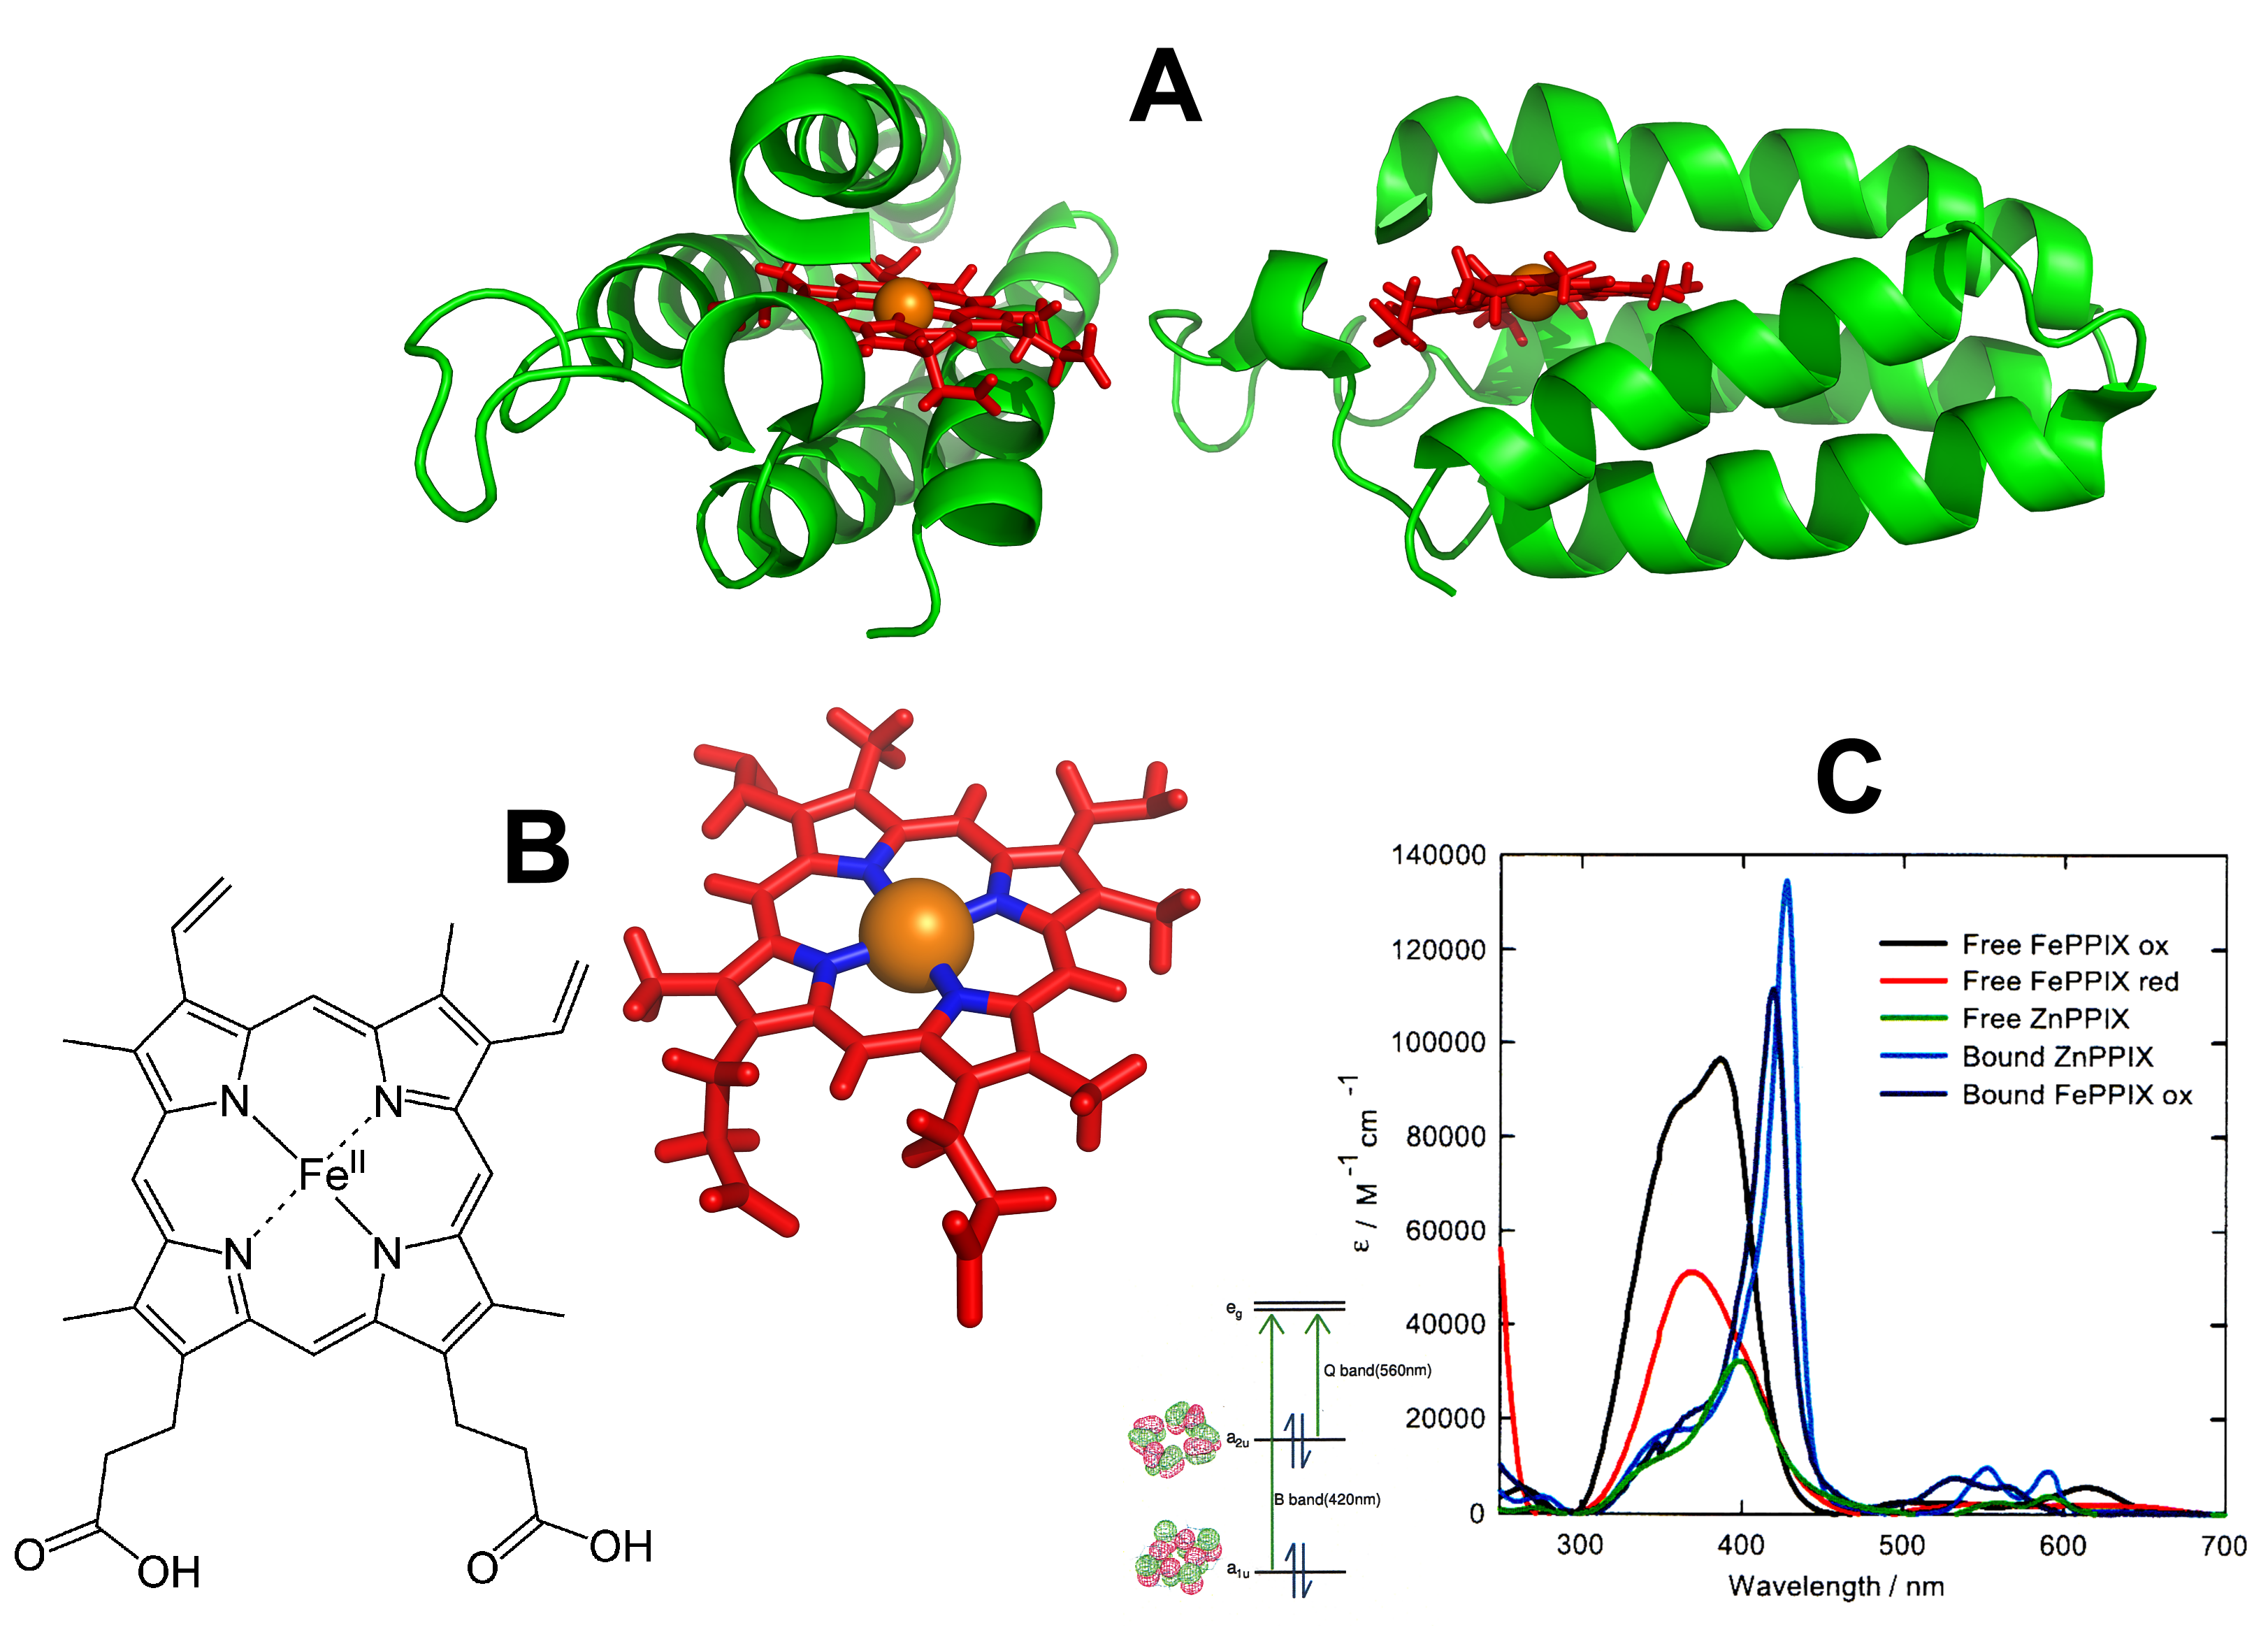
\includegraphics[width=137.4mm]{Images/haemStructure.png}
	\caption[Haem Structure]{A fancy image.}
	\label{fig:haemStructure}
\end{figure}
\end{verbatim}

\vspace{2ex}

\begin{figure}[!th]
	\centering
	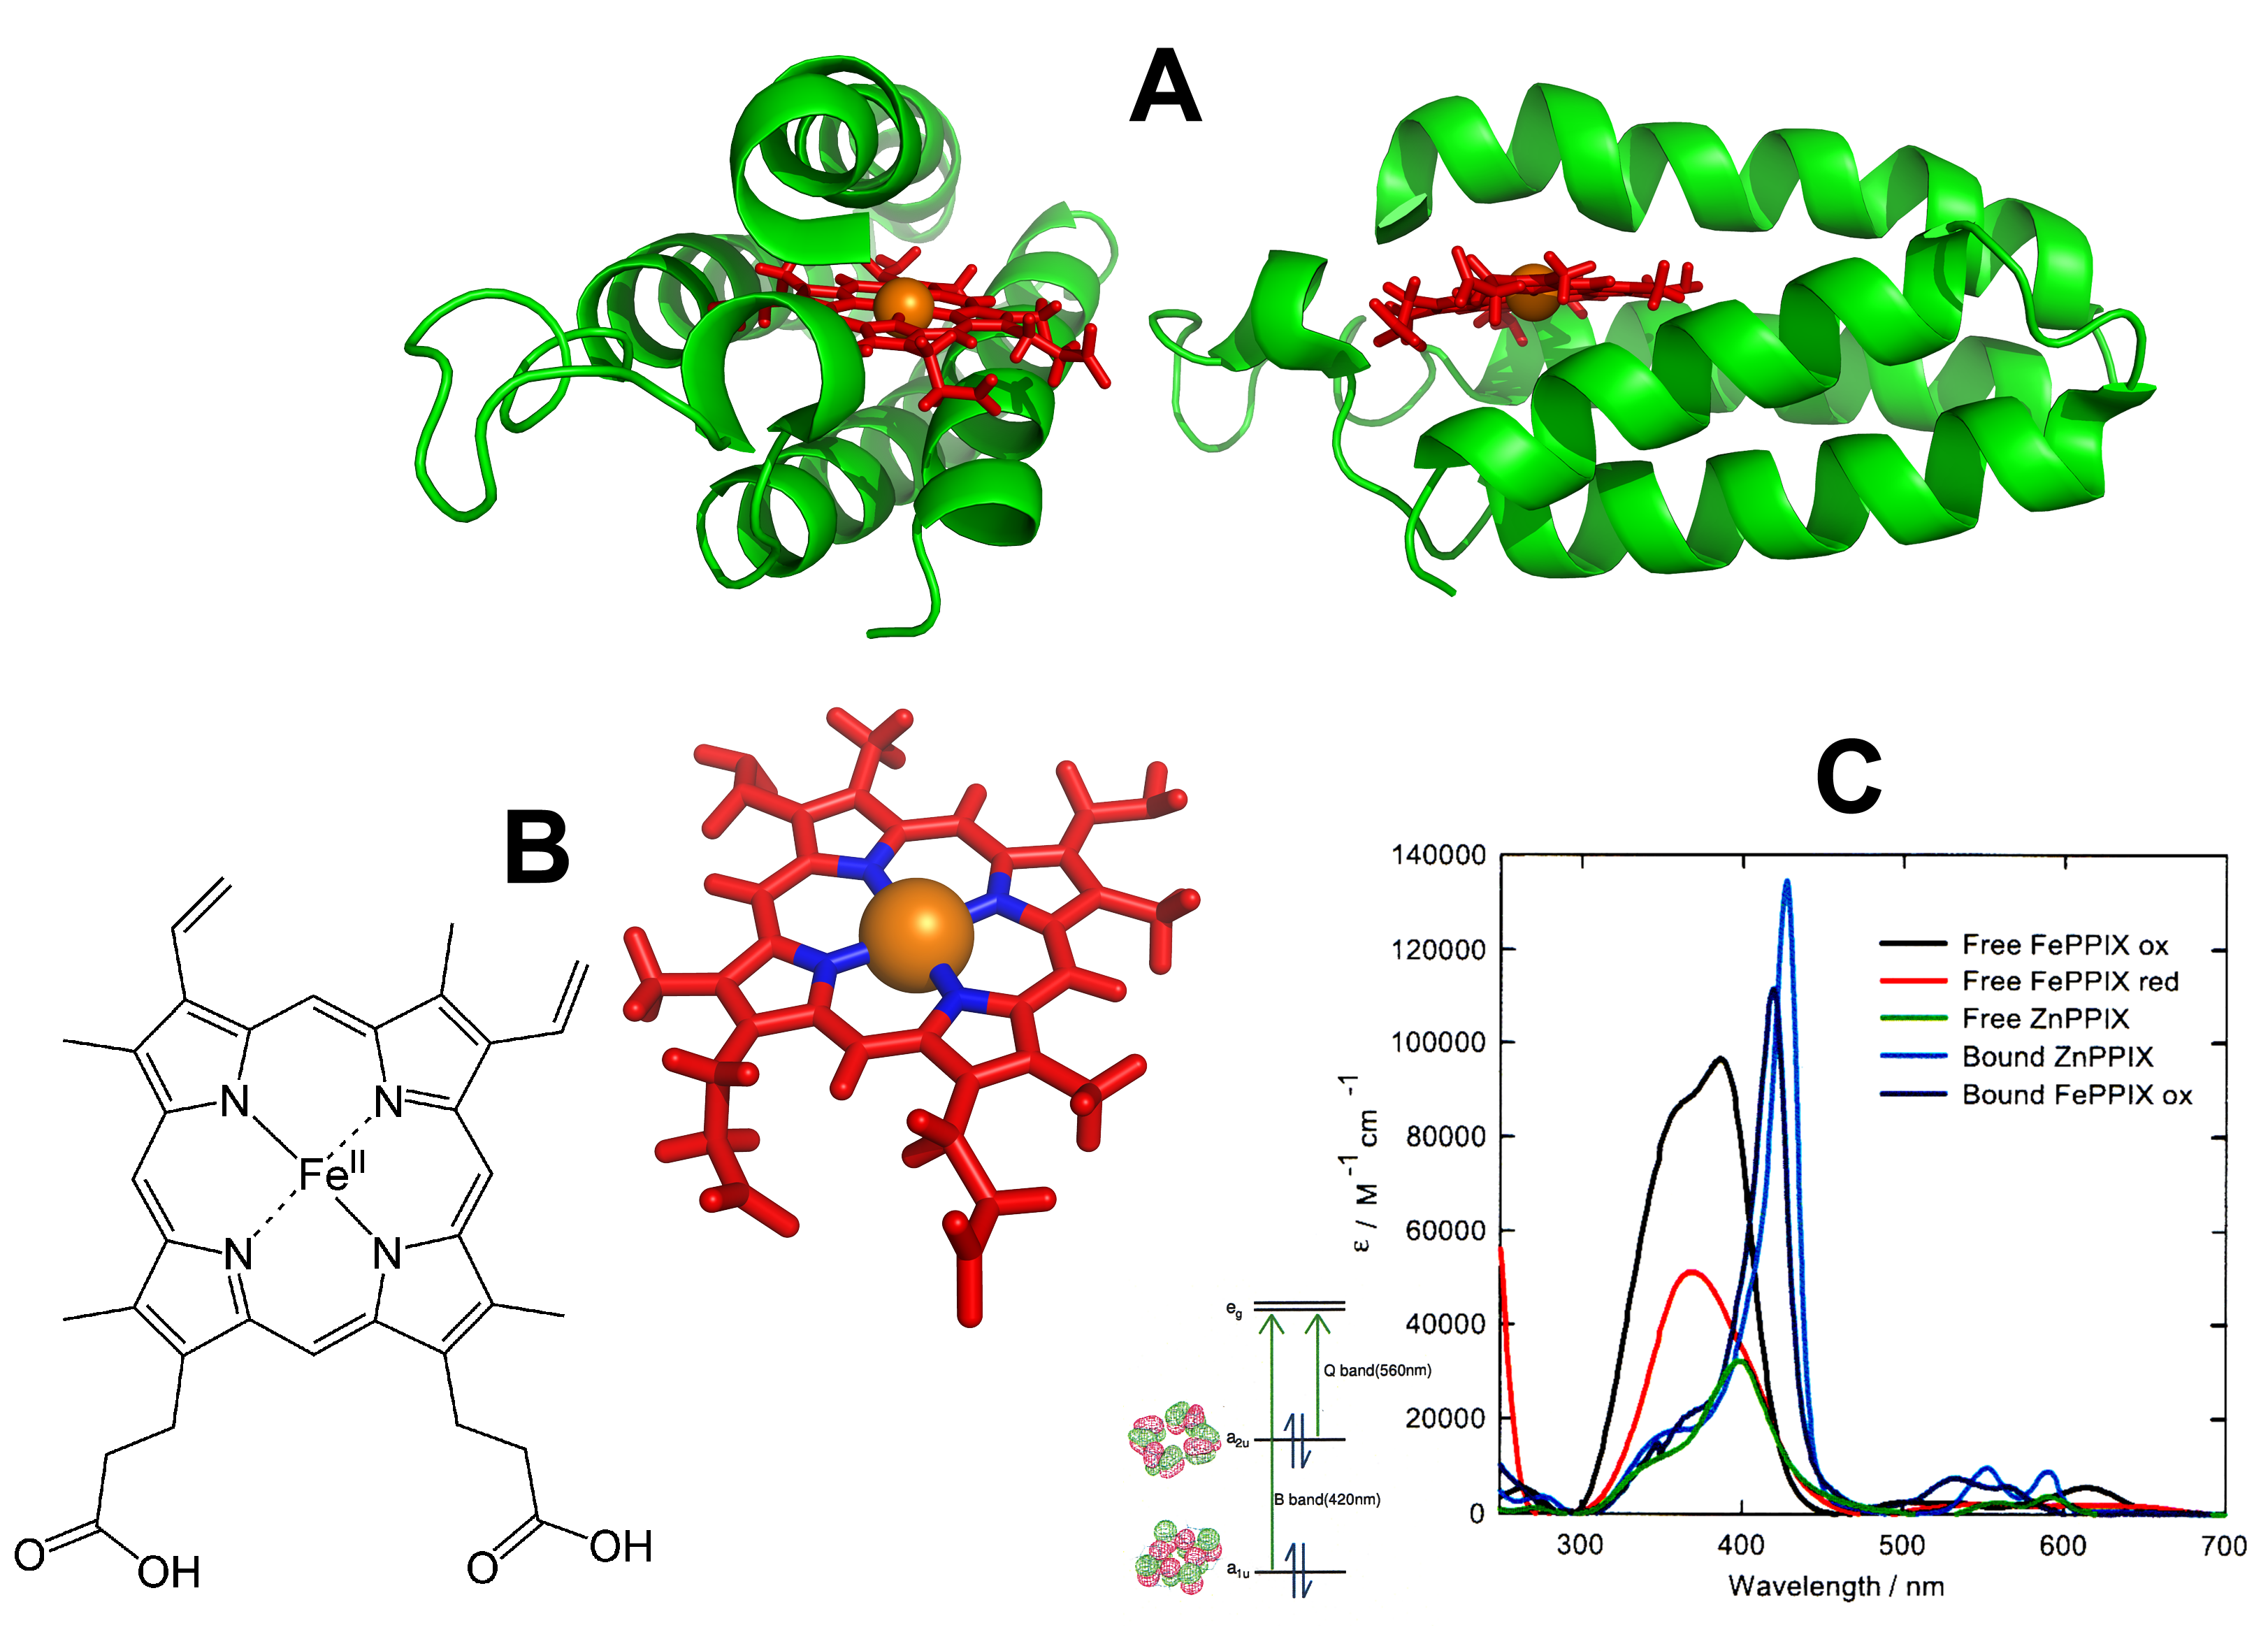
\includegraphics[width=137.4mm]{Images/haemStructure.png}
	\caption[Haem Structure]{A fancy image from Chris' Thesis.}
	\label{fig:haemStructure}
\end{figure}

In this example the command {\textbackslash}includegraphics tells LaTeX to look in the directory `Images' and incorporate the file called `haemStructure.png' into the final document while setting the width to 137.4mm.  This command can be used to resize a graphical file using the height or width parameter as shown. You must specify the units which can be pt, ex, em, mm, cm and so on. LaTeX recognises a very wide variety of standard units and graphics formats. The command is part of the graphicx package and so in the preamble you must include the command {\textbackslash}usepackage\{graphicx\}.

Many packages have been written to provide new commands. For example the `subfigure' package enables you to place separate images or files in the same figure side by side while giving them their own label. However, in this document we only concentrate on the very basics.

\section{Floating Environments}

Both tables and figures are examples of a `floating environments' which means LaTeX decides where to put them. 

The mysterious [!tbh] letters give guidance to LaTeX about roughly where the figure or table is  allowed to be, but in general they can move a long way from where you position them within your text file.  The letters in the square bracket can be t, h or b which stand for top, here or bottom.  If you don't specify any letters LaTeX defaults to [t].

LaTeX will always preserve the order in which figures appear.  If it cannot find a type setting solution, then it may move the float to it's own page, and combine it with other figures. If it still can't fit that in for some reason then it moves the float to the end of the document.  This has the effect of pushing all the remaining floating environments to the end of the document also.

The exclamation mark instructs LaTeX to ``try harder'' at putting the float where you told it to. Often you must play around to ensure the float positioning is acceptable, but usually this can be achieved by stretching or shrinking the image slightly using the size parameter, re-ordering text, judicial applications of the {\textbackslash}pagebreak command or by shouting loudly and slapping the computer monitor about. Note that it is better to resize the image using the original program that was used to create the image. Also using vector graphics can assist be useful (e.g. eps files) because they are designed to scale better.
\chapter{The Chapter on Making Chapters}
\label{sec:Chapters}

Right. LaTeX forces you to structure your document. There a series of simple commands for achieving this:

\vspace*{2ex}

{\textbackslash}chapter\{chapterName\}

{\textbackslash}section\{sectionName\}

{\textbackslash}subsection\{subsectionName\}

{\textbackslash}subsubsection\{subsubsectionName\}

\vspace*{2ex}

Easy enough. At the start of each chapter or section just issue one of these commands to name the section and LaTeX will present the chapter heading in the right style of font, which will be the same style of all the other heading names at that level of hierarchy throughout the document. In addition LaTeX assigns a number to that section. For example, this chapter was created using the command:

\vspace*{2ex}

{\textbackslash}chapter\{The Chapter on Making Chapters\} 

\vspace*{2ex}

LaTeX assigns the correct chapter number to each chapter in turn and then puts it in the table of contents, as you can see by looking at the table of contents! Easy.

\pagebreak
\section{The Section About Sections}
\label{sec:Section}
I think you're getting the hang of this. This section was created using the command {\textbackslash}section\{The Section About Sections\}. It appears in the table of contents as section \ref{sec:Section}.

\subsection{The Sub-Section About Sub-Sections}
\label{sec:SubSection}
Now you're really getting the hang of this. This subsection was created using the command {\textbackslash}subsection\{The Sub-Section About Sub-Sections\}. 

\subsubsection{The Sub-Sub-Section About Sub-Sub-Sections}
\label{sec:SubSubSection}
Now you're really getting the hang of this. but.. caught you out! This subsubsection doesn't have a number!  Ha Ha! It was created using the command {\textbackslash}subsubsection\{The Sub-Sub-Section About Sub-Sub-Sections\} in the same vein as all the other subsections/chapters etc. Here we have stopped the depth of the section numbering at the second level with the command:

\vspace*{2ex}

{\textbackslash}setcounter\{secnumdepth\}\{2\}

\vspace*{2ex}

Easy. WYSIWYM.  LaTeX does what you tell it to do. This is both a blessing and a curse.

\pagebreak
\section*{The Section About Sections That Don't Appear in the Table of Contents}
\label{sec:InvisibleSection}
Ok. Now we're throwing a spanner in the works. This section was created using the command:

\vspace*{2ex}

{\textbackslash}section*\{The Section About Sections That Don't Appear in the Table of Contents\}. 

\vspace*{2ex}

Notice how LaTeX has not assigned a number to the section and it doesn't appear in the table of contents. The effect of the * is to suppress the inclusion of a chapter, section or subsection in the automatic numbering. Easy. You can do this at any level. This is useful for things like prefaces, tables of contents or acknowledgements which you may or may not wish to have an entry in the main contents table. Up to you. It's your thesis. Don't just copy me.

\section{A Small Point About Numbering}

In this section notice how the numbering starts from where it left off before we suppressed the numbering on the previous section. Easy. WYSIWYM.
\pagebreak
\section{The Section About Internal Referencing}
\label{sec:InternalReferencing}

There are two related commands:

\vspace*{2ex}

{\textbackslash}label\{labelName\} 

{\textbackslash}ref\{labelName\}

\vspace*{2ex}


The {\textbackslash}label\{\} command allows you to create a label in a particular environment\footnote{That's right. Chapters, Sections and sub-sections etc are environments!}. The label won't appear in the final document. It's just a label which makes it easy to refer back to any particular environment elsewhere in the document. The {\textbackslash}ref\{\} command enables you to insert a reference anywhere in the document to any label in the document.  For example this is section \ref{sec:InternalReferencing}. The names you use in a label can be anything you like but musn't contain whitespace or special characters. I used the two commands:

\vspace*{2ex}

{\textbackslash}label\{sec:InternalReferencing\}

{\textbackslash}ref\{sec:InternalReferencing\}.

\vspace*{2ex}

The astute among you will realise that LaTeX has to read the document several times. Once to find the labels and then again to populate the references with the correct numbers. So you have to compile a latex document twice to get the referencing right. If there is a missing label or you refer to something that doesn't exist then latex inserts a convenient ? at that point. So hunting for queries is useful way of finding broken references. Latex issues warnings when it finds broken references.

As you create a document you will find yourself putting labels in all over the place so choose a sensible naming convention to help you remember the label names.

Each type of environment (equations, figures, tables, sections etc) has its own independent numbering system.  So when you choose your label name it's a good idea to have an identifier for that type of environment.  I have my own convention for label names which I use to help me remember references. E.g.   sec:SectionAboutCats. Eqn:EquationAboutCats,  Fig:FigureAboutCats and so on. This means you can differentiate between referring to the section or the figure more easily, even though they are about the same thing.

So Internal Referencing is a doddle. Easy!
\chapter{External Referencing}

Referencing is usually performed using a separate program called BibTex.  This program understands the file format .bib.

To create a reference within your document first you must create a .bib file by exporting your list of references from which ever referencing software you used, such as endnote, mendeley or whatever you use.

You can refer to an entry in the .bib file using the {\textbackslash}cite\{ref:Name\} command. the identifier `ref:Name' is the unique identifier which is the first line of each item included in your bibliography file.

For example, open the file LaTexCourseBib.bib in the bibliography directory. The first entry has the identifier `Horcas2007'.  This can be invoked as follows:


\begin{verbatim}
For example, this interesting fact\cite{Horcas2007}, is a cracking example.
\end{verbatim}

For example, this interesting fact\cite{Horcas2007}, is a cracking example.

During compilation latex and bibtex co-operate. During the first compilation latex generates a list of references that it needs.  During the second compilation bibtex populates the details from the .bib file into a shorter, ordered .bib file. The third compilation inserts markers at the right place in the main file and the fourth compilation generates the final list of references. Thus the compilation sequence is latex, bibtex, latex, latex.

The style of the referencing format can be changed using the command {\textbackslash}bibliographyStyle\{\}. e.g. the style used in this document is cjfthesisv1.bst which is invoked by 

\begin{verbatim}
\bibliographystyle{Bibliography/cjfthesisv1}
\end{verbatim}

The location of the list of references in the document is specified by issuing the {\textbackslash}bibliography\{\} command which also specifies the master bibliography file.

\begin{verbatim}
\bibliography{Bibliography/LaTeXCourseBib}
\end{verbatim}




\chapter{Organising Your Files}
One of the drawbacks of word is that the figures and tables are included within the document which becomes very very clunky quite quickly and once it reaches around 100Mb it becomes unwieldy and hard to export. One of that advantages of LaTeX is that the files are all text files and so are very light on resources and are easy to email around the place.

However, sometimes it can be difficult to navigate through a single text file, so if you had a huge document then it becomes difficult to find your way around.  One way of circumnavigating this problem is to break the file up into smaller files. As long as LaTeX knows where to look you can have a file for each logical sub-division of your document.

Therefore it is worth spending a bit of time at the beginning of a large project deciding how you wish to break up your LaTex Files and organise them neatly and tidily.  You can then tell LaTex where to look for the files using the following command:

\vspace*{2ex}
{\textbackslash}include\{fileName\}
\vspace*{2ex}

\pagebreak
\section{Linking a File}
We are now going to copy part of the tutorial file into a separate files and link it the main file.  Because this could go wrong it is sensible to back up tutorial.tex as something else. So save a copy called `tutorialOriginal.tex' for safe keeping. Then follow the following instructions.

\begin{enumerate}
\item Create a new file called MyFirstPage.tex
\item Select and Cut out the first chapter of Tutorial.Tex
\item Paste the first chapter into MyFirstPage.tex
\item Save both tutorial.tex and MyFirstPage.tex
\item Then add {\textbackslash}include\{MyFirstPage\} in tutorial.tex where the text used to be before you cut it out. We don't need to add the `.tex' because LaTeX can only include `.tex' files.
\item compile tutorial.tex and view the PDF
\end{enumerate}

The final PDF should look exactly the same as it was! except we now have a separate file for one of the chapters.

\pagebreak
\section{Creating A Class File}
We can also save our preamble in a separate file called a class file. This makes your main document much easier to understand.  To make it work we need to use the {\textbackslash}LoadClass\{\} command as follows: 

\begin{enumerate}
\item Create another new file and save it as TutorialStyle.cls
\item Copy the preamble of tutorial.tex into the new file. Starting with the {\textbackslash}documentclass{} command and copy right up to, but not including, the {\textbackslash}begin{document} command. Delete the preamble in the original document.
\item Save TutorialStyle.cls and tutorial.tex
\item Modify the first line of TutorialStyle.cls by replacing the word `document' with the word `Load'.
\item Add a new first line of tutorial.tex to use your new style class {\textbackslash}documentclass\{TutorialStyle\}
\item Save both files.
\end{enumerate}

\subsection{Sanity Check}

The first line of TutorialStyle.cls should now be:

\begin{verbatim}
\LoadClass[12pt, oneside, a4paper]{book}
\end{verbatim}
\vspace{2ex}

The first line of tutorial.tex should be:

\begin{verbatim}
\documentClass{TutorialStyle}
\end{verbatim}
\vspace{2ex}

We have just created what is called a style file. You can use this style file as a generic preamble for other documents as well. Compile tutorial.tex.  Nothing should have changed in the final PDF.


\pagebreak
\section{The Structure of this Document}

Lets now look at how I've organised this document. It is identical to my thesis because it started out life as my thesis. I usurped the structure and simply replaced the headings and content to make a kind of reference manual for this introductory course. This document therefore is three things:

\begin{enumerate}
\item An example thesis structure to work from.
\item The LaTeX files which were used to create it can be used as a template for a thesis.
\item It is also a convenient introductory latex manual!
\end{enumerate}

\vspace*{2ex}
Groovy huh?

\section{The Master File}

There is a master file where LaTeX begins the compilation procedure. This contains the {\textbackslash}documentclass command needed to set the ball rolling. Within the file there are a series of {\textbackslash}include\{\} commands, one for each Chapter, which tell LaTeX where to find the files containing each chapter.

The subfiles cannot be compiled on their own because they do not contain the {\textbackslash}documentclass, {\textbackslash}begin\{document\} or {\textbackslash}end\{document\} commands. Lets us look in more detail at the master file and we will learn some new LaTeX commands.

\singlespacing
\pagebreak
\begin{verbatim}
\documentclass{Style/LatexCourseStyle}

\begin{document}
\setcounter{secnumdepth}{2}
\setcounter{tocdepth}{1}

\frontmatter
\onehalfspacing
\thispagestyle{empty}

\begin{center}
\vspace*{\stretch{1}}

\hrule height 2pt
\vspace*{2ex}
{\Huge\textbf{Towards the Ability to Make Super Duper LaTeX Documents}\par}
\vspace*{2ex}
\hrule height 2pt
\vspace*{10ex}
{
\includegraphics[height=40mm]{Images/UnivShield}\par}
\vspace*{10ex}
{\large\textbf{Christopher~James~Forman}\par}
\vspace*{2ex}
{\large{Department Of Chemistry}\par}
\vspace*{2ex}
{\large{University of Cambridge}\par}
\vspace*{5ex}
{\large{This dissertation is submitted for the degree of \textit{Doctor of Philosophy}}\par}
\vspace*{5ex}
{\large{\today}\par}

\vspace*{\stretch{2}}
\end{center}
\chapter*{Declaration}

\vfill

This dissertation is the result of my own work and includes nothing which is the outcome of work done in collaboration except where specifically indicated in the text. It is not substantially the same as any that I have submitted for a degree or diploma or other qualification at any other University and no part has already been, or is concurrently being, submitted for any degree, diploma, or other qualification. It does not exceed 60,000 words, including tables, footnotes, bibliography and appendices.\par

\vspace{10ex}

\begin{flushright}
Signature: \rule[0pt]{60mm}{0.5pt}

\vspace{5ex}

Date: \rule[0pt]{60mm}{0.5pt}
\end{flushright}

\vfill
\chapter*{Acknowledgments}
\subsection*{Family}
Mum. Dad. Pet Dog.

\subsection*{Scientific Collaborations}
Dr A.N.Other at uni of blah for samples and instrument time etc. My Amazing Lab Chums.

\subsection*{Scientific Support}
My amazing lab chums.

\subsection*{General Assistance}
Cleaner, My amazing lab chums.

\subsection*{Financial Support}
Bank, Tax payer. My amazing lab chums.

\subsection*{Moral Support}
My Amazing Lab chums.

\subsection*{Academic Inspiration}
Netwon, My super. My Amazing Lab Chums.

\subsection*{Everyone else}
My Amazing Lab Chums.

\chapter*{Summary}
This document is a handbook for introducing you to LaTeX. It contains a bit of background about the history and philosophy of LaTeX.  However, it concentrates on providing a guided practical introduction to the basic techniques such as 
\begin{itemize}
\item Lists
\item Mathematical and chemical equations
\item Tables
\item Figures
\item Chapters and Sections
\item Linking to other files in large documents
\item Referencing
\end{itemize}

The handbook is also presented in the style of a thesis. This means that source files provided on the introductory course and available from the department web page are a convenient template for a thesis.

More details on specific aspects of LaTeX can be found at the departmental LaTeX page which can be found here:

 http://www-ch-int.ch.private.cam.ac.uk/latex/about

\chapter*{Abbreviations}

\begin{longtable}{r >{\rule{0pt}{3ex}}l<{\rule[-1.5ex]{0pt}{0pt}}}
ADP & Adenosine Diphosphate\\
(nc/c)AFM & (non-contact/conducting) Atomic Force Microscopy\\
ATP & Adenosine Triphosphate \\
\end{longtable}
\tableofcontents
\listoftables
\listoffigures

\mainmatter
\renewcommand{\sectionmark}[1]{\markright{\thesection \ #1}{}}
\chapter{Overview}
\label{chap:overview}
\section{LaTeX: The answer to everything.}
LaTeX is typsetting program that takes an input file of marked up text and then, with a user defined set of rules, typesets a beautifully crafted output file that can be easily printed (e.g. a pdf). 

\subsection{Advantages}

The advantages of this method are manifold:

\begin{itemize}

\item Use any text editor to view the source document.
\item More time can be spent working on the content and not worrying about how text or figures interact in the layout until later on.
\item LaTeX uses consistent rules throughout a document
\item LaTeX sorts out basic typesetting automatically
\item Changes can be introduced globally with very little effort
\item Document structure is explicit
\item Documents can be professionally typeset and look great
\item You are forced to structure your documents correctly.
\item Mathematical equations, like $E=mc^2$ or $\imath\hbar\frac{\partial}{\partial t}\Phi (x, t) = \hat{H}\Phi (x, t)$ can be produced almost as fast as typing (if you know the commands!).
\end{itemize}

\subsection{Disadvantages}
The disadvanatges of this method are also manifold:
\begin{itemize}
\item You don't see the output as you go.
\item Steep learning curve.
\item Documents are harder to edit by a second author (unless they are adept at LaTeX too). This can be mitigated using version control, which makes group authoring processes superior to word.
\item The program never works quite the way you want it to and learning how to influence it can be problematic and subtle.
\item Although intended to save work the principle of 'conservation of work' means that you simply transform problems associated with WYSISYG approaches to problems associated with WYSIWYM approaches!
\item You can go blind trying to determine the difference between wiggly and smooth brackets if your editors font isn't large enough.
\end{itemize}

\subsection{On balance?}
If it's so rubbish, why use LaTeX?

\begin{itemize}
\item Large documents are much more easily handled. 
\item In general it is quicker to debug a LaTeX document than typeset an entire thesis manually. 
\item Technical information such as tables, equations and figures are integrated much more smoothly than with word.
\end{itemize}

\section{How does it work?}

The raw text is interspersed with commands, preceded by a \textbackslash, which tell LaTeX what to do with the text. For example you can \textbf{make it bold}, \emph{italic}, or \underline{underlined} with the commands {\textbackslash}textbf\{\}, {\textbackslash}emph\{\} or {\textbackslash}underlined\{\}. More on commands in a moment...



\chapter{My First Page}

\section{The Very Beginning}
The very simplest LaTeX document might look like this:

\begin{verbatim}
\documentclass[a4paper,12pt]{article}
\begin{document}
Hello World.
\end{document}
\end{verbatim}

\pagebreak
\thispagestyle{empty}
Hello World.
\pagebreak
\subsection{Break Down}
What's all the gobbledegook around my simple message???

In LaTeX we intersperse text and commands.  Commands are preceded by a \textbackslash. For example the first line in a LaTeX document \underline{\textbf{\emph{must}}} be:

\begin{verbatim}
\documentclass[options]{class}
\end{verbatim}

Where the word ''class'' may be substituted for one of many things such as: article, proc, minimal, report, book, letter, memoir, slides, beamer.

Similarly, and completely generally in LaTeX speak, the square brackets denote the existence of optional parameters. Each individual command can take its own parameters and for the ''{\textbackslash}documentclass'' command there are options for controlling font size, font family, landscape, oneside, twosided, page size and so on. These options will persist throughout the entire document. For example the document class command for this document, (which is likely to be like the one you would use for a thesis), would be:

\begin{verbatim}
\documentclass[12pt, oneside, a4paper]{book}
\end{verbatim}

Other options include:

\begin{itemize}
\item {10pt, 11pt, 12pt (default is 10pt).}
\item {letterpaper, legalpaper, a4paper, executivepaper, a5paper, b5paper}
\end{itemize}
and so on.

\pagebreak
\section{Can I start typing please?}

After we have set up the document we can start actual work on our document. So we must tell LaTeX that what follows is to be interpreted as a document.  The command {\textbackslash}begin can take many different parameters and is a command to enter what is known, in LaTeX speak, as 'an environment'. Thus the commands:
\begin{verbatim}
\begin{document}

\end{document}
\end{verbatim}

tells LaTeX to enter and leave the document environment, and thus constitute the outer limits of our document file. Other environments include the equation environment, the itemize environment, the figure environment and so on. These will be encountered in due course.

Every part of the LaTeX file is therefore within an environment of specific type and the content within each environment consists of commands or text.

That's basically it.

So let's get on with it shall we...

\pagebreak
\section{The ground rules}
\begin{quote}
Hold on, hold on, hold on my son.

First the lessons.

Then the fun!
\end{quote}
Dr Seuss.

\subsection{Spaces}
Whitespace characters, such as blank or tab, are treated uniformly as space by LaTeX. Several consecutive whitespace characters are treated as one single space. Whitespace at the start of a line is generally ignored, and a single line break is treated as whitespace. An empty line between two lines of text defines the end of a paragraph. Several empty lines are treated the same as one empty line. The text below is an example.

\begin{verbatim}
It does not matter whether you
enter one or several             spaces
after a word. The final result will be typeset beautifully
according    to     precise rules.




An empty line starts a new
paragraph. Note the indentation on the first line of the paragraph, 
except at the beginning of the section. 
\end{verbatim}

\vspace*{2ex}
\vspace*{2ex}

It does not matter whether you
enter one or several             spaces
after a word. The final result will be typeset beautifully
according    to     specific rules.




An empty line starts a new
paragraph. Note the indentation on the first line of the paragraph, except at the beginning of the section. 

\pagebreak
\subsection{Special Characters}
The symbols 

\# \$ \% \textasciicircum{} \& \_ \{ \} \~{} \textbackslash

are reserved characters that either have a special meaning under LaTeX or are unavailable in all the fonts. If you enter them directly in your text, they will normally not print, but rather make LaTeX do strange things.

To overide the special meanings of these symbols and allow them to produced within your text you may use the following sequences:
\begin{verbatim}
\# \$ \% \textasciicircum{} \& \_ \{ \} \~{} \textbackslash
\end{verbatim}

Other symbols and many more can be printed with special commands in mathematical formulae or as accents.

The backslash character '\textbackslash' cannot be entered by adding another backslash in front of it ( \textbackslash\textbackslash); because this sequence means ''linebreak''.

The command \textbackslash\~{}\{\} produces a tilde which is placed over the next letter. For example \textbackslash\~{}\{n\} gives \~{n}. To produce just the character \~{}, use \textbackslash\~{}\{\} which places a \~{} over an empty box.

Similarly, the command \textbackslash\textasciicircum{} produces a hat over the next character, for example \textbackslash\textasciicircum\{o\} produces \^{o}.

\pagebreak
\section{Preamble}
After the {\textbackslash}documentclass command we add ''preamble''. Here we load special features that we will use throughout our document to expand on the basic capabilities of LaTex. These are contained in units called ''packages'' which we can tell our LaTeX compiler to download by using the command ''{\textbackslash}include\{packageName\}''. 

There are many repositories of such packages on the web. Your compiler generally knows where to look and most standard packages are included with any install. For example, to include a special set of typesetting instructions to handle chemical equations we can grow our simple document with a single command like this:

\begin{verbatim}
\documentclass[a4paper,12pt]{article}
\usepackage[version=3]{mhchem}
\begin{document}
Hello World!

We all need \ce{H2O}.

I'm less fussed about \ce{^{235}_{92}U+}.

\end{document}
\end{verbatim}

\vspace{2ex}

\pagebreak
\thispagestyle{empty}
Hello World!

We all need \ce{H2O}.

I'm less fussed about \ce{^{235}_{92}U+}.
\pagebreak

Here we have loaded a package called: "`mhchem"' which took the option ''[version=3]''. This is a package for drawing chemical equations easily and it has it's own instruction manual which you can follow easily. It is included in the bundle of files for this course.

Other things we can do in the premable within LaTeX are to redefine existing commands or create our own personal commands. These can be stored in a file called the 'style file' which we can load at the beginning of our document, in place of our documentclass. More about this later on...


\subsection{Comments}
It is often useful to comment your LaTeX documents. You can leave yourself amusing, sarcastic messages that won't get printed out in the final document. Use this to make your own notes as the course progresses.

To get a comment use the \% command, which tells LaTeX to ignore the rest of the line, the line break and all the white space at the beginning of the next line, for example, we may add to our continually evolving document...

\begin{verbatim}
\documentclass[a4paper,12pt]{article}
\usepackage[version=3]{mhchem}
\begin{document}
Hello World!

%All humans need water and I would like 
%to include this concept in my arguments.
We all need \ce{H2O}.

%Uranium 235 is toxic, which is why I don't want to consume it... 
I'm less fussed about \ce{^{235}_{92}U+}.

\end{document}
\end{verbatim}

\vspace{4ex}
Hello World!

%All humans need water and I would like to include this concept in my arguments.
We all need \ce{H2O}.

%Uranium 235 is toxic, which is why I don't want to consume it... 
I'm less fussed about \ce{^{235}_{92}U+}.

\pagebreak
\section{Compiling}
Once the document is finished you can compile it. Your compiler will depend on the platform that you use. In the PWF we are using winEDT to edit the documents (a LaTeX front end) and texlive2008 which is the compiler itself. I use MiKTex and the front end texCenter.  There is no need to use a front end. If you prefer you can use a simple text editor and a command line.

the recommended distributions are:
\begin{itemize}
\item MiKTeX or TeX Live for Windows
\item TeX Live for Unix/Linux
\item MacTeX or TeX Live for Mac OS.
\end{itemize}

Once you have installed your software and got it working, written your source code and tried to compile it, there will nearly always be something wrong with your file. 

Any errors will be highlighted in the console window or error output box of your front end.  Some front ends dump the running commentary which LaTeX produces into a text file for easy reading afterwards.

In a compile attempt (successful or otherwise) LaTeX may produce the following files:

projectname.aux

projectname.bbl

projectname.lof

projectname.lot

projectname.txt

projectname.toc

projectname.dvi

These are interim files (toc= table of contents, bbl = bibliography etc). To be honest I have no idea what half of these things contain.  You only need the .tex file and a compiler with the right packages installed to produce them again.

Some versions of LaTeX only produce DVI files and you then need to convert the dvi file to a PDF or download a dvi viewer. You can also convert DVI files to PS files and then view them.  The good thing about front ends is that you can set them up to produce PDFs directly.

OK. So we have now produced a silly document but we understand it.  Now lets get on with learning how to make our own documents.



\chapter{Lists}
Lists are great.  The command {\textbackslash}begin\{\} can be used to enter a list environment.  For example:

\begin{verbatim}
\begin{itemize}
\item cat
\item dog
\item horse
\end{itemize}
\end{verbatim}

Produces:

\begin{itemize}
\item cat
\item dog
\item horse
\end{itemize}

\pagebreak
We can also replace the bullet points with numbers using the enumerate keyword.

\begin{verbatim}
\begin{enumerate}
\item cat
\item dog
\item horse
\end{enumerate}
\end{verbatim}

\begin{enumerate}
\item cat
\item dog
\item horse
\end{enumerate}

\pagebreak
and we can use the description keyword which does this:
\begin{verbatim}
\begin{description}
\item[Cat] a lovely furry creature with a cute nose and whiskers.
\item[Dog] Another furry creature that smells rather well; 
           its olfactory power stems from its nasal dampness.
\item [Horse] A large stinky creature with sideways facing eyes.
\end{description}
\end{verbatim}

\begin{description}
\item[Cat] a lovely furry creature with a cute nose and whiskers.
\item[Dog] Another furry creature that smells rather well; its olfactory power stems from its nasal dampness.
\item [Horse] A large stinky creature with sideways facing eyes.
\end{description}
\chapter{Maths Equations}

\section{Producing Beautiful Looking Mathematics}

One of the best features about LaTeX is `maths mode'.  For example the schrodinger equation can be produced as follows:

\vspace*{2ex}

\begin{center}
\begin{math}
\imath\hbar\frac{\partial}{\partial t}\Phi (x, t) = \hat{H}\Phi (x, t)
\end{math}
\end{center}

\vspace*{2ex}

\begin{verbatim}
\begin{math}
\imath\hbar\frac{\partial}{\partial t}\Phi(x,t)=\hat{H}\Phi(x,t)
\end{math}
\end{verbatim}

There are a number of ways to switch on maths mode.  The first, as above, is with the {\textbackslash}begin\{math\} environment. You can also enter mathmode inline using the \$ symbol. For example typing in \$y=ax\textasciicircum{}2+bx+c\$ yields $y=ax^2+bx+c$.  Another way is to enter the equation environment which enables you to number equations so you can then refer to them later in the text.

\begin{equation}
y(t)= \sin \left(\frac{{\alpha}t}{2\pi} + \phi_0\right)
\label{eqn:MadeUpNonsense}
\end{equation}

\vspace*{2ex}
\begin{verbatim}
\begin{equation}
y(t)= \sin \left(\frac{{\alpha}t}{2\pi} + \phi_0\right)
\end{equation}
\end{verbatim}.

\section{Basic Maths Mode}
Once in maths mode there is a kind of text based code for writing down your equations.  Here are the most basic symbols to get you going.
\begin{center}
\begin{tabular}{cc}
\toprule
Final Result & LaTeX Code \\
\cmidrule(){1-2}
$a+b$ & a+b \\
$a-b$ & a-b \\
$ab$ & ab \\
$a*b$ & a*b \\
$a \times b$ & a {\textbackslash}times b \\
$a \cdot b$ & a {\textbackslash}cdot b \\
$\frac{a}{b}$ & {\textbackslash}frac\{a\}\{b\} \\ 
$a^b$ & a\textasciicircum{}b \\
$a_b$ & a\_b \\
$\sin a$ & {\textbackslash}sin a  (same for cos, tan)\\
$ sin a$ & sin a \\
$\sqrt{a}$ & {\textbackslash}sqrt\{a\} \\
$\left( a \right) $ & {\textbackslash}left( a {\textbackslash}right)\\ 
$\left[ a \right]$ & {\textbackslash}left[ a {\textbackslash}right]\\ 
$\alpha$ & {\textbackslash}alpha \\
$\pi$ & {\textbackslash}pi \\
\bottomrule
\end{tabular}
\end{center}

A full treatise on maths mode is not practical here. There are lots of online tutorials and summaries of symbols. It just takes a bit of practice and you can build up equations really easily. It's straight forward to learn new stuff once you've done it a few times.

\pagebreak
\section{Equation Arrays}
Sometimes you need to arrange several equations vertically, referencing individual lines separately and aligning the equations on the $=$ sign. This can be achieved with equation arrays as follows:

\begin{eqnarray}
A\left( x\right) & = & \frac{x^2+2x+1}{x+1} \\
& = & \frac{\left(x+1\right)\left(x+1\right)}{x+1} \nonumber\\
& = & x+1 \nonumber\\
B(x,t) & = & \frac{e^{\left(\imath\omega_0 t + kx\right)}}{4\pi\epsilon_0}
\end{eqnarray}

\begin{verbatim}
\begin{eqnarray}
A\left( x\right) & = & \frac{x^2+2x+1}{1+x} \\
& = & \frac{\left(x+1\right)\left(x+1\right)}{1+x} \nonumber\\
& = & x+1 \nonumber\\
B(x,t) & = & \frac{e^{\left(\imath\omega_0 t + kx\right)}}{4\pi\epsilon_0}
\end{eqnarray}
\end{verbatim}

\begin{itemize}
\item Note the \& symbols. This tells LaTeX where to align the equations. There must be the same number of \& symbols in each line.
\item Note the \textbackslash\textbackslash ~at the end of each line except the last one. This symbol tells LaTeX to add another row in the array.  If you put it on the last line you get an empty row at the bottom of the array.
\item Note the {\textbackslash}nonumber command which suppresses line numbering for that line.
\item Note that equation number carries on from equation \ref{eqn:MadeUpNonsense} in the previous section.
\end{itemize}

\section{Maths Packages}

Maths mode comes as standard in LaTeX, however you can download packages that buff up your maths symbol set. For example neat vector notation comes in the package `vector'. e.g. {\textbackslash}uuvec\{T\} yields $\uuvec{T}$.

\begin{verbatim}
\usepackage{amssymb}
\usepackage{amsmath}
\usepackage{vector}
\end{verbatim}


\chapter{Chemical Equations}
The mhchem package means you can do basic stuff very easily using {\textbackslash}ce\{\}. For example:

\vspace{2ex}
\begin{verbatim}
\ce{CO2 + C -> 2CO}
\ce{CO2 + C <- 2CO}
\ce{CO2 + C <=> 2CO}
\ce{A-B=C#D\sbond E\dbond F\tbond G}
\end{verbatim}
\vspace{2ex}
\begin{center}
\ce{CO2 + C -> 2CO}

\ce{CO2 + C <- 2CO}

\ce{CO2 + C <=> 2CO}

\ce{A-B=C#D\sbond E\dbond F\tbond G}
\end{center}

\vspace{2ex}
You can also use math mode within chemical equations.
\vspace{2ex}

\begin{center}
\ce{$x\,$ Na(NH4)HPO4 ->[\Delta] (NaPO3)_{$x$} + $x\,$ NH3 ^ + $x\,$ H2O}
\end{center}

\begin{verbatim}
\ce{$x\,$ Na(NH4)HPO4 ->[\Delta](NaPO3)_{$x$} + $x\,$ NH3 ^ + $x\,$ H2O}
\end{verbatim}

And you can number chemical reactions as well by using the math mode equation environment.

\begin{equation}
\ce{CO2 + C <=> 2CO}
\end{equation}

\begin{verbatim}
\begin{equation}
\ce{CO2 + C <=> 2CO}
\end{equation}
\end{verbatim}

However, this will number mathematical and chemical equations using the same number system. There is a discussion in the mhchem pdf which shows you how to number chemical and mathematical equations independently. It's a bit complex and involves you creating your own type of environment... bit beyond the intro level of this course...
\chapter{Tables}
Tables are big business in Latex.  I use these packages to help me.

\begin{verbatim}
\usepackage{multirow}
\usepackage{booktabs}
\usepackage{dcolumn}
\end{verbatim}

Here's an example table

\begin{table}[!hb]
 \centering
	\begin{tabular}{@{}rccc@{~}r@{.}l*3{r@{.}l@{~}r@{.}l}D{.}{\cdot}{2,1}}
	\toprule
	\multicolumn{1}{c}{Fibre Type}
	& N 
	& M 
	&\multicolumn{3}{c}{$L_t$ (nm)}
	&\multicolumn{4}{c}{$R_t$ (nm)}
	&\multicolumn{4}{c}{$d_t$ (nm)}
	&\multicolumn{4}{c}{${\Delta}Z_t$ (nm)}
	&\multicolumn{1}{c}{~}\\
\cmidrule(lr){1-1}
\cmidrule(lr){2-2}
\cmidrule(lr){3-3}
\cmidrule(lr){4-6}
\cmidrule(lr){7-10}
\cmidrule(lr){11-14}
\cmidrule(lr){15-18}
  SS Twisted & 5 & 4 & 313 &\multicolumn{2}{c}{(122)} & 5&7 &(1&6)  & 5&4 &(1&0)  &  150&5 &(63&1) &\multicolumn{1}{c}{~} \\
  \multicolumn{19}{c}{~}\\
  %\cmidrule(lr){3-18}
  &
  &
 	&\multicolumn{3}{c}{$L_s$ (nm)} 
 	&\multicolumn{4}{c}{$R_s$ (nm)}
 	&\multicolumn{4}{c}{$W_s$ (nm)}
 	&\multicolumn{4}{c}{${\Delta}Z_s$ (nm)}
 	&\multicolumn{1}{c}{${\Delta}Z_{e}$ (nm)}\\
\cmidrule(lr){4-6}
\cmidrule(lr){7-10}
\cmidrule(lr){11-14}
\cmidrule(lr){15-18}
\cmidrule(lr){19-19}
  SS Spiral& 32 & 7 &123&(31&6)&11&4&(3&3)&11&1&(2&6)&32&9&(22&2)&26.9\\
  SSB Spiral& 64&18 &106&(22&9)&10&8&(2&7)&9&8&(1&8)&28&2&(8&1)&22.7\\
	%\midrule
  BSS Spiral&37 &19 &110&(44&9)&13&4&(3&0)&12&9&(1&8)&27&1&(9&1)&21.5\\
	%\midrule
  SSSB Spiral&26& 6 &104&(23&9)&13&3&(2&6)&16&4&(3&4)&29&9&(11&1)&22.5\\
	\bottomrule
	\end{tabular}	
	\caption[Basic Fibre Dimensions by TEM]{A funky table from my thesis.}
	\label{tab:BasicXSBFibreDimensionsTEM}
\end{table}

\pagebreak
Here's what the code looks like:
\begin{verbatim}
\begin{table}[!hb]
 \centering
	\begin{tabular}{@{}rccc@{~}r@{.}l*3{r@{.}l@{~}r@{.}l}D{.}{\cdot}{2,1}}
	\toprule
	\multicolumn{1}{c}{Fibre Type}
	& N 
	& M 
	&\multicolumn{3}{c}{$L_t$ (nm)}
	&\multicolumn{4}{c}{$R_t$ (nm)}
	&\multicolumn{4}{c}{$d_t$ (nm)}
	&\multicolumn{4}{c}{${\Delta}Z_t$ (nm)}
	&\multicolumn{1}{c}{~}\\
\cmidrule(lr){1-1}
\cmidrule(lr){2-2}
\cmidrule(lr){3-3}
\cmidrule(lr){4-6}
\cmidrule(lr){7-10}
\cmidrule(lr){11-14}
\cmidrule(lr){15-18}
  SS Twisted & 5 & 4 & 313 &\multicolumn{2}{c}{(122)} & 5&7 &(1&6)  & 5&4 &(1&0)  &  150&5 &(63&1) &\multicolumn{1}{c}{~} \\
  \multicolumn{19}{c}{~}\\
  %\cmidrule(lr){3-18}
  &
  &
 	&\multicolumn{3}{c}{$L_s$ (nm)} 
 	&\multicolumn{4}{c}{$R_s$ (nm)}
 	&\multicolumn{4}{c}{$W_s$ (nm)}
 	&\multicolumn{4}{c}{${\Delta}Z_s$ (nm)}
 	&\multicolumn{1}{c}{${\Delta}Z_{e}$ (nm)}\\
\cmidrule(lr){4-6}
\cmidrule(lr){7-10}
\cmidrule(lr){11-14}
\cmidrule(lr){15-18}
\cmidrule(lr){19-19}
  SS Spiral& 32 & 7 &123&(31&6)&11&4&(3&3)&11&1&(2&6)&32&9&(22&2)&26.9\\
  SSB Spiral& 64&18 &106&(22&9)&10&8&(2&7)&9&8&(1&8)&28&2&(8&1)&22.7\\
	%\midrule
  BSS Spiral&37 &19 &110&(44&9)&13&4&(3&0)&12&9&(1&8)&27&1&(9&1)&21.5\\
	%\midrule
  SSSB Spiral&26& 6 &104&(23&9)&13&3&(2&6)&16&4&(3&4)&29&9&(11&1)&22.5\\
	\bottomrule
	\end{tabular}	
	\caption[Basic Fibre Dimensions by TEM]{A funky table from my thesis.}
	\label{tab:BasicXSBFibreDimensionsTEM}
\end{table}
\end{verbatim}

\pagebreak

\section{Tables Made Easy}
Here is a simple table followed by the code that produced it.

\begin{center}
\begin{tabular}{lcr}
anchovy & banana & carrot \\
dog & apple & fennel \\
goat & strawberry & potato
\end{tabular}

\vspace*{2ex}

\begin{verbatim}
\begin{tabular}{lcr}
anchovy & banana & carrot \\
dog & apple & fennel \\
goat & strawberry & potato
\end{tabular}
\end{verbatim}
\end{center}

\vspace*{2ex}

The tabular environment is a special case of the ''array'' environment for distributing content uniformly across a region of the page.  This ability has already been exploited to align mathematical equations. For now though look at the first line.

\vspace*{2ex}

\begin{verbatim}
\begin{tabular}{lcr}
\end{verbatim}

\vspace*{2ex}

This command tells LaTeX to enter the tabular environment. The letters l, c and r in the curly braces tell LaTeX to create a table with three columns in which the first column is left justified, the second column is centered and the third column is right justified. Lets add a fourth column and this time center justify all the columns.

\begin{center}
\begin{tabular}{cccc}
anchovy & banana & carrot & Johnny\\
dog & apple & fennel & Pete\\
goat & strawberry & potato &
\end{tabular}

\vspace*{2ex}

\begin{verbatim}
\begin{tabular}{cccc}
anchovy & banana & carrot & Johnny\\
dog & apple & fennel & Pete\\
goat & strawberry & potato &
\end{tabular}
\end{verbatim}
\end{center}

\vspace*{2ex}

Each row in the table is a list of items separated by the {\&} symbol. The end of each row is denoted by \textbackslash\textbackslash.  The last row in the table doesn't have a \textbackslash\textbackslash. You do not have to have data between the ampersands but you must have the right number of ampersands to match the number of columns that LaTeX is expecting.

\subsection{Adding Borders To Tables}
\label{sec:vertLines}
Tables should never have vertical lines. No professionally typeset table contains vertical lines. Do not put vertical lines in your tables. That said it is easy to do.

\begin{center}
\begin{tabular}{|c|c|c|c|}
anchovy & banana & carrot & Johnny\\
dog & apple & fennel & Pete\\
goat & strawberry & potato &
\end{tabular}

\vspace*{2ex}

\begin{verbatim}
\begin{tabular}{|c|c|c|c|}
anchovy & banana & carrot & Johnny\\
dog & apple & fennel & Pete\\
goat & strawberry & potato &
\end{tabular}
\end{verbatim}
\end{center}

\vspace*{2ex}

Tables should have neatly headed columns with the heading for each field separated from the data by horizontal lines. The {\textbackslash}toprule, {\textbackslash}cmidrule{} and {\textbackslash}bottomrule commands from the booktabs package are useful for controlling horizontal lines.

\begin{center}
\begin{tabular}{cccc}
\toprule
Ingredient 1 & Ingredient 2 & Ingredient 3 & Source \\
\cmidrule(){1-4}
anchovy & banana & carrot & Johnny\\
dog & apple & fennel & Pete\\
goat & strawberry & potato & \\
\bottomrule
\end{tabular}

\vspace*{2ex}

\begin{verbatim}
\begin{tabular}{cccc}
\toprule
Ingredient 1 & Ingredient 2 & Ingredient 3 & Source \\
\cmidrule(){1-4}
anchovy & banana & carrot & Johnny\\
dog & apple & fennel & Pete\\
goat & strawberry & potato & \\
\bottomrule
\end{tabular}
\end{verbatim}
\end{center}

Note that when using the {\textbackslash}bottomrule command you must add the \textbackslash\textbackslash ~symbol to the last line of data.  The last line of the table is now buried within the {\textbackslash}bottomrule command.

\pagebreak
\subsection{The {\textbackslash}cmidrule Command}
This useful and versatile command takes a bunch of options to control subtleties like only putting lines across some of the columns, or not quite making them cross the full width of the column. The (lr) option trims the left and right ends of the lines off. For example:

\begin{center}
\begin{tabular}{ccccc}
\toprule
Recipe Version & Ingredient 1 & Ingredient 2 & Ingredient 3 & Source \\
\cmidrule(lr){1-1}
\cmidrule(l){2-2}
\cmidrule(){3-3}
\cmidrule(r){4-4}
\cmidrule(lr){5-5}
10.1 & anchovy & banana & carrot & Johnny\\
1.34 & dog & apple & fennel & Pete\\
709.23 & goat & strawberry & potato & \\
\bottomrule
\end{tabular}

\vspace*{2ex}

\begin{verbatim}
\begin{tabular}{ccccc}
\toprule
Recipe Version & Ingredient 1 & Ingredient 2 & Ingredient 3 & Source \\
\cmidrule(lr){1-1}
\cmidrule(l){2-2}
\cmidrule(){3-3}
\cmidrule(r){4-4}
\cmidrule(lr){5-5}
10.1 & anchovy & banana & carrot & Johnny\\
1.34 & dog & apple & fennel & Pete\\
709.23 & goat & strawberry & potato & \\
\bottomrule
\end{tabular}
\end{verbatim}
\end{center}

\pagebreak
\subsection{Aligning Decimal Points}
Note that the decimal points don't line up in the new column ''Recipe Version'' in the previous section. There is a way round this with the DColumn package.

\begin{center}
\begin{tabular}{D{.}{\cdot}{4,4}cccc}
\toprule
Recipe Version & Ingredient 1 & Ingredient 2 & Ingredient 3 & Source \\
\cmidrule(lr){1-1}
\cmidrule(lr){2-2}
\cmidrule(lr){3-3}
\cmidrule(lr){4-4}
\cmidrule(lr){5-5}
10.1 & anchovy & banana & carrot & Johnny\\
1.34 & dog & apple & fennel & Pete\\
709.23 & goat & strawberry & potato & \\
\bottomrule
\end{tabular}

\vspace*{2ex}

\begin{verbatim}
\begin{center}
\begin{tabular}{D{.}{\cdot}{4,4}cccc}
\toprule
Recipe Version & Ingredient 1 & Ingredient 2 & Ingredient 3 & Source \\
\cmidrule(lr){1-2}
\cmidrule(lr){3-3}
\cmidrule(lr){4-4}
\cmidrule(lr){5-5}
\cmidrule(lr){6-6}
10.1 & anchovy & banana & carrot & Johnny\\
1.34 & dog & apple & fennel & Pete\\
709.23 & goat & strawberry & potato & \\
\bottomrule
\end{tabular}
\end{verbatim}
\end{center}

The DColumn package defines a new type of column which can be invoked placing a capital D in the {\textbackslash}tabular command which defines the table. If defined using a D, then the column is placed in mathmode. D takes four parameters: D\{a\}\{b\}\{c,d\} where a is the symbol which is to be aligned, b is the symbol with which to replace the aligning character, and {c,d} must be integers which indicate LaTeX should have up to c white space characters before the aligning character and d afterwards, thereby defining the position of the number within the column. The command {\textbackslash}cdot prints a special type of mathmode symbol which is a dot that is vertically shifted and larger than a normal period e.g.: $\cdot$ 

\pagebreak
\subsection{Final Table Trick}
DColumn forces the column to be in mathmode which is why the heading ''Recipe Version'' was typeset in italics in the previous section. Indeed LaTeX tried to interpret the heading of the table as a number to be aligned.  We can over ride this behaviour by using the {\textbackslash}multicolumn command to locally impose a different type of justification and temporarily disable mathmode as follows:

\begin{center}
\begin{tabular}{D{.}{\cdot}{4,4}cccc}
\toprule
\multicolumn{1}{c}{Recipe Version}& Ingredient 1 & Ingredient 2 & Ingredient 3 & Source \\
\cmidrule(lr){1-1}
\cmidrule(lr){2-2}
\cmidrule(lr){3-3}
\cmidrule(lr){4-4}
\cmidrule(lr){5-5}
10.1 & anchovy & banana & carrot & Johnny\\
1.34 & dog & apple & fennel & Pete\\
709.23 & goat & strawberry & potato & \\
\bottomrule
\end{tabular}

\vspace*{2ex}

\begin{verbatim}
\begin{tabular}{D{.}{\cdot}{4,4}cccc}
\toprule
\multicolumn{1}{c}{Recipe Version} & Ingredient 1 & Ingredient 2 & Ingredient 3 & Source \\
\cmidrule(lr){1-1}
\cmidrule(lr){2-2}
\cmidrule(lr){3-3}
\cmidrule(lr){4-4}
\cmidrule(lr){5-5}
10.1 & anchovy & banana & carrot & Johnny\\
1.34 & dog & apple & fennel & Pete\\
709.23 & goat & strawberry & potato & \\
\bottomrule
\end{tabular}
\end{verbatim}
\end{center}

This introduces you to the multicolumn command which you can use to span text over several columns.  The format is \textbackslash{multicolumn}\{n\}\{j\}\{text\} where n is the number of columns to span. j is the justification: either l,c or r and text is the text to add. There is also a similar command \textbackslash{multirow}.

\pagebreak
\section{Numbering Tables}
To tell LaTeX to assign a number to a table and add it to the list of tables you must use the {\textbackslash}begin\{table\} command to tell LaTeX to create a table environment as follows:

\begin{table}[!bh]
\centering
\begin{tabular}{D{.}{\cdot}{4,4}cccc}
\toprule
\multicolumn{1}{c}{Recipe Version}& Ingredient 1 & Ingredient 2 & Ingredient 3 & Source \\
\cmidrule(lr){1-1}
\cmidrule(lr){2-2}
\cmidrule(lr){3-3}
\cmidrule(lr){4-4}
\cmidrule(lr){5-5}
10.1 & anchovy & banana & carrot & Johnny\\
1.34 & dog & apple & fennel & Pete\\
709.23 & goat & strawberry & potato & \\
\bottomrule
\end{tabular}
\caption[Table of Banned Recipes]{Recipes that ought to be banned.}
\label{tab:Recipes}
\end{table}
\begin{verbatim}
\begin{table}[!bh]
\centering
\begin{tabular}{D{.}{\cdot}{4,4}cccc}
\toprule
\multicolumn{1}{c}{Recipe Version}& Ingredient 1 & Ingredient 2 & Ingredient 3 & Source \\
\cmidrule(lr){1-1}
\cmidrule(lr){2-2}
\cmidrule(lr){3-3}
\cmidrule(lr){4-4}
\cmidrule(lr){5-5}
10.1 & anchovy & banana & carrot & Johnny\\
1.34 & dog & apple & fennel & Pete\\
709.23 & goat & strawberry & potato & \\
\bottomrule
\end{tabular}
\caption[Table of Banned Recipes]{Recipes that ought to be banned.}
\label{tab:Recipes}
\end{table}
\end{verbatim}

In the table environment the {\textbackslash}caption[text1]\{text2\} command adds a caption, where text1 appears in the list of tables at the beginning of the document and text2 is the local caption.  The label command creates a label with which to reference the table e.g. Table \ref{tab:Recipes} is a table of recipes that have been made up to illustrate how to use tables in LaTeX. We also use the {\textbackslash}centering command to center the table and caption within the table environment. We could also use the {\textbackslash}begin\{center\} and {\textbackslash}end\{center\} commands.
\chapter{Adding Figures To Your Document}

\section{My First Figure}

Adding figures is easy in LaTeX. You just create a figure environment which is much the same as the table environment. For example:

\begin{verbatim}
\begin{figure}[!th]
	\centering
	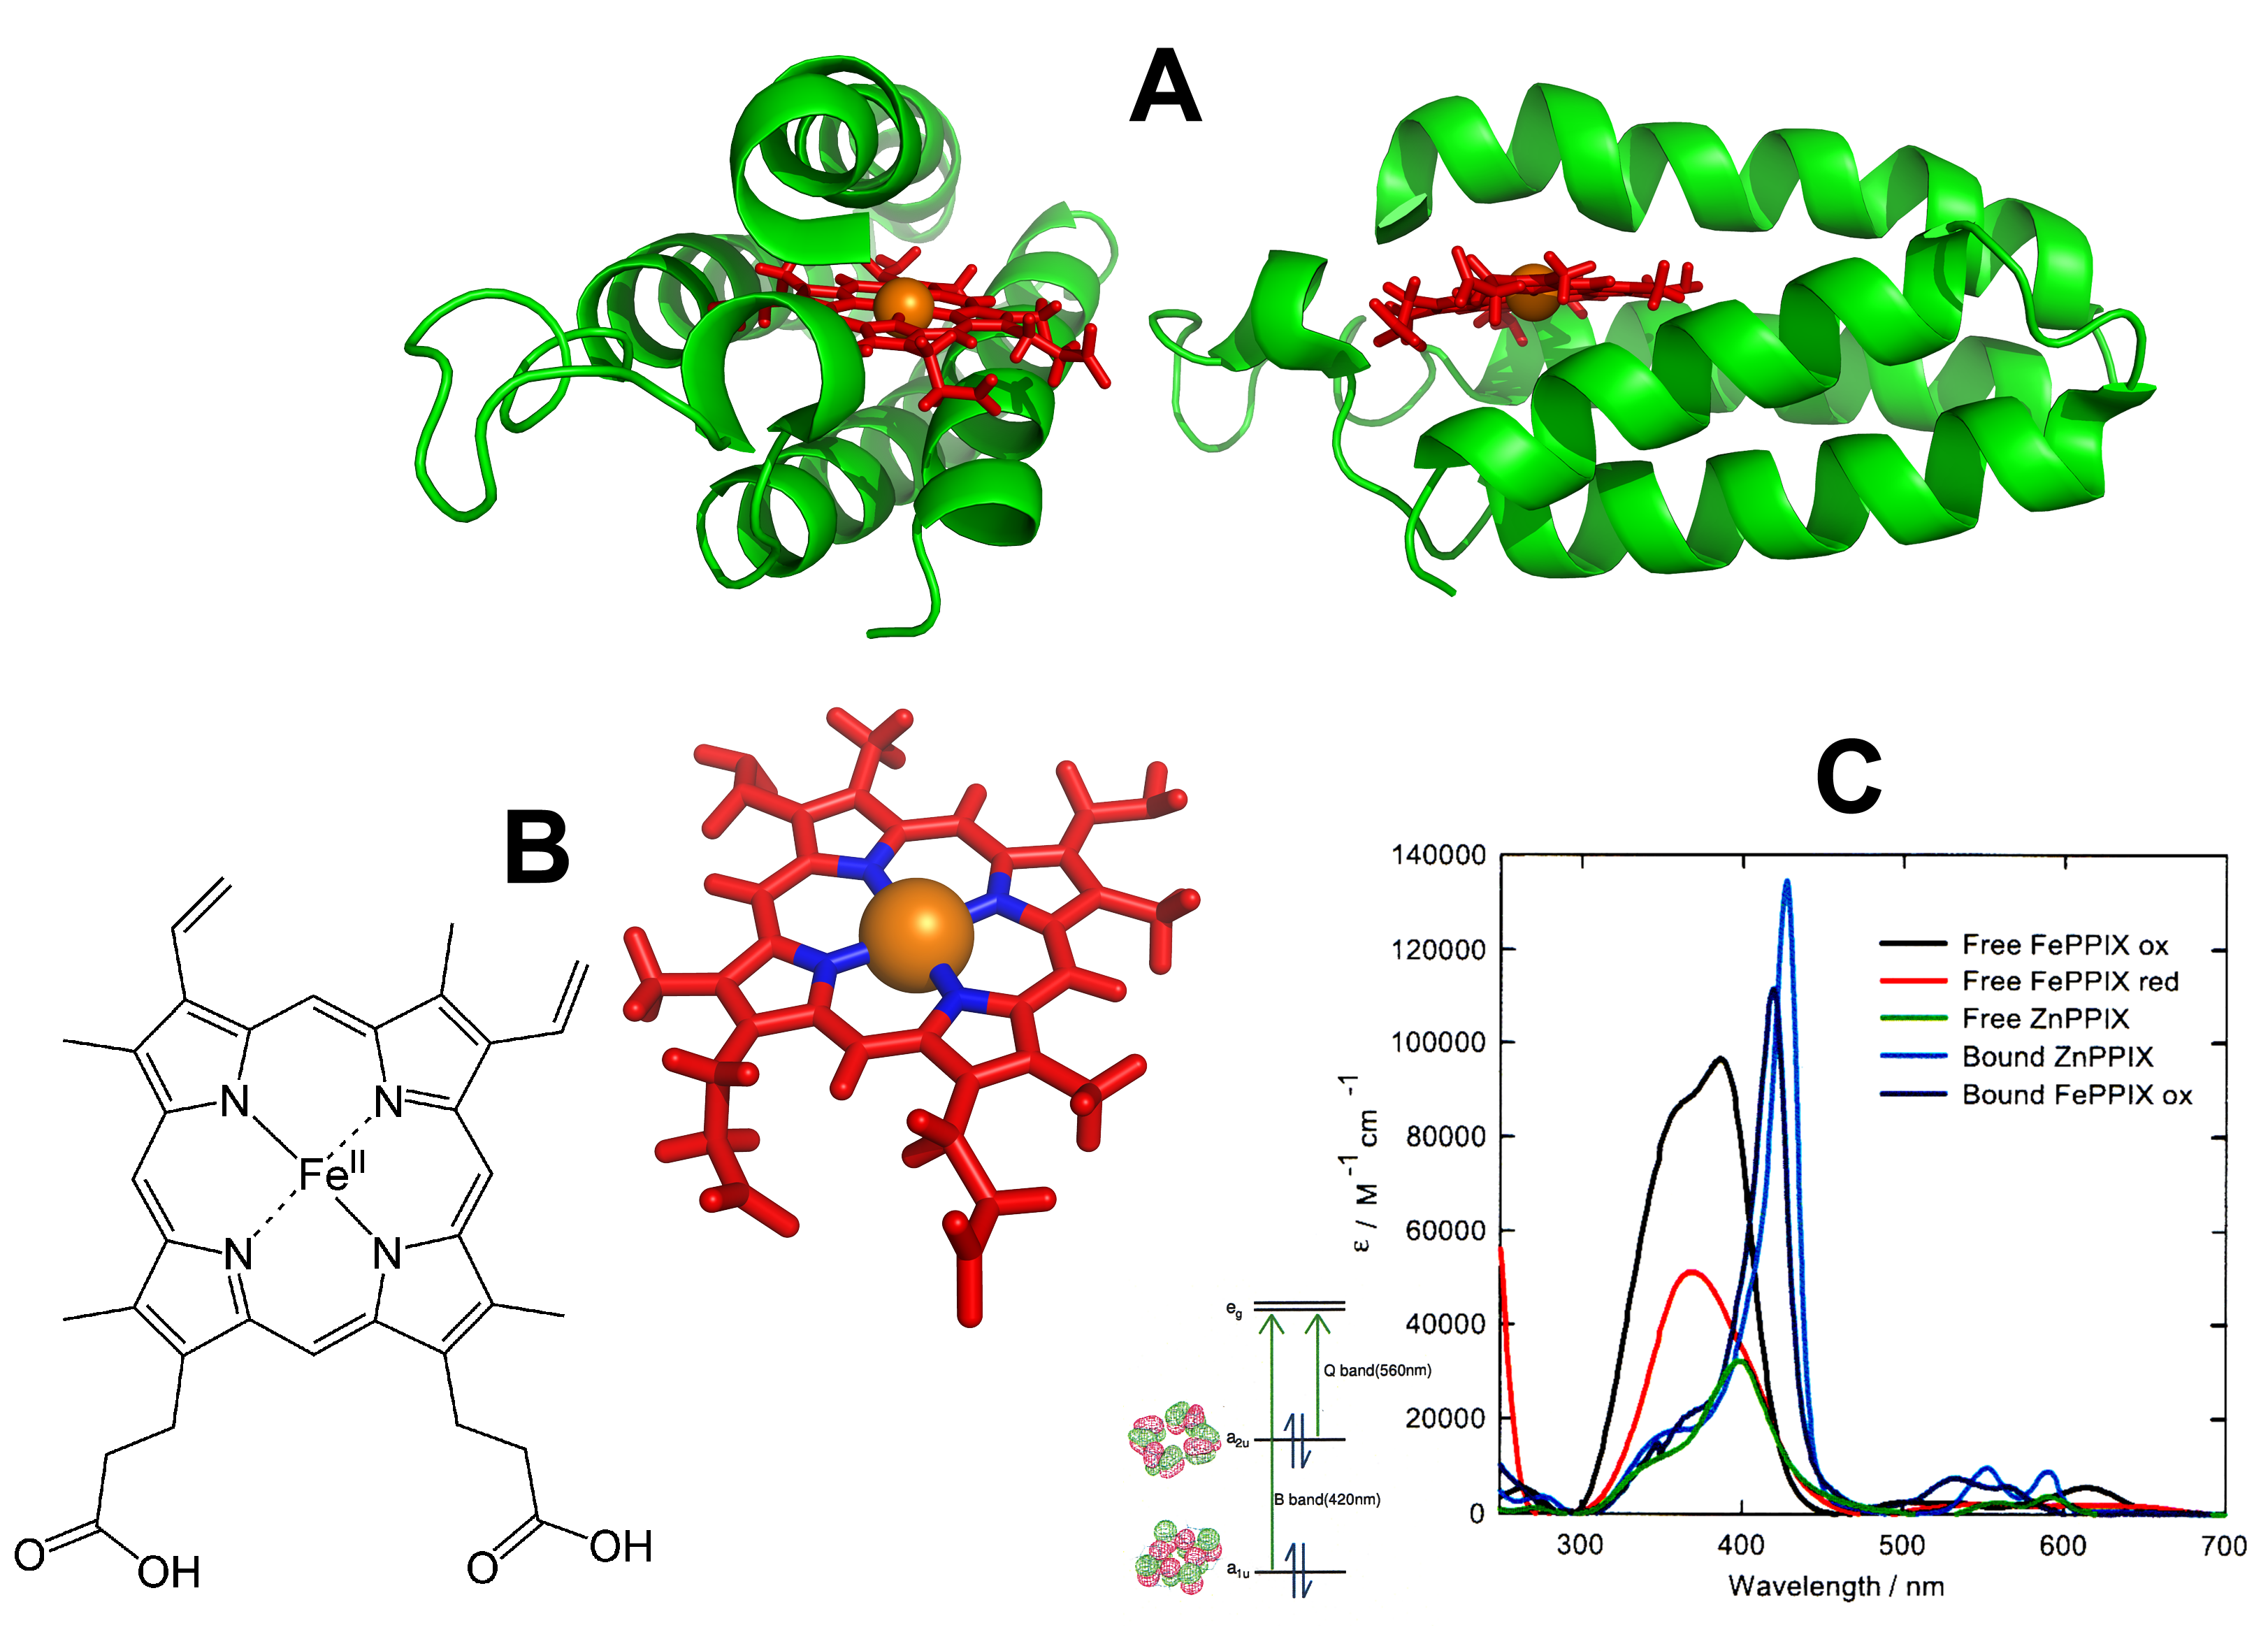
\includegraphics[width=137.4mm]{Images/haemStructure.png}
	\caption[Haem Structure]{A fancy image.}
	\label{fig:haemStructure}
\end{figure}
\end{verbatim}

\vspace{2ex}

\begin{figure}[!th]
	\centering
	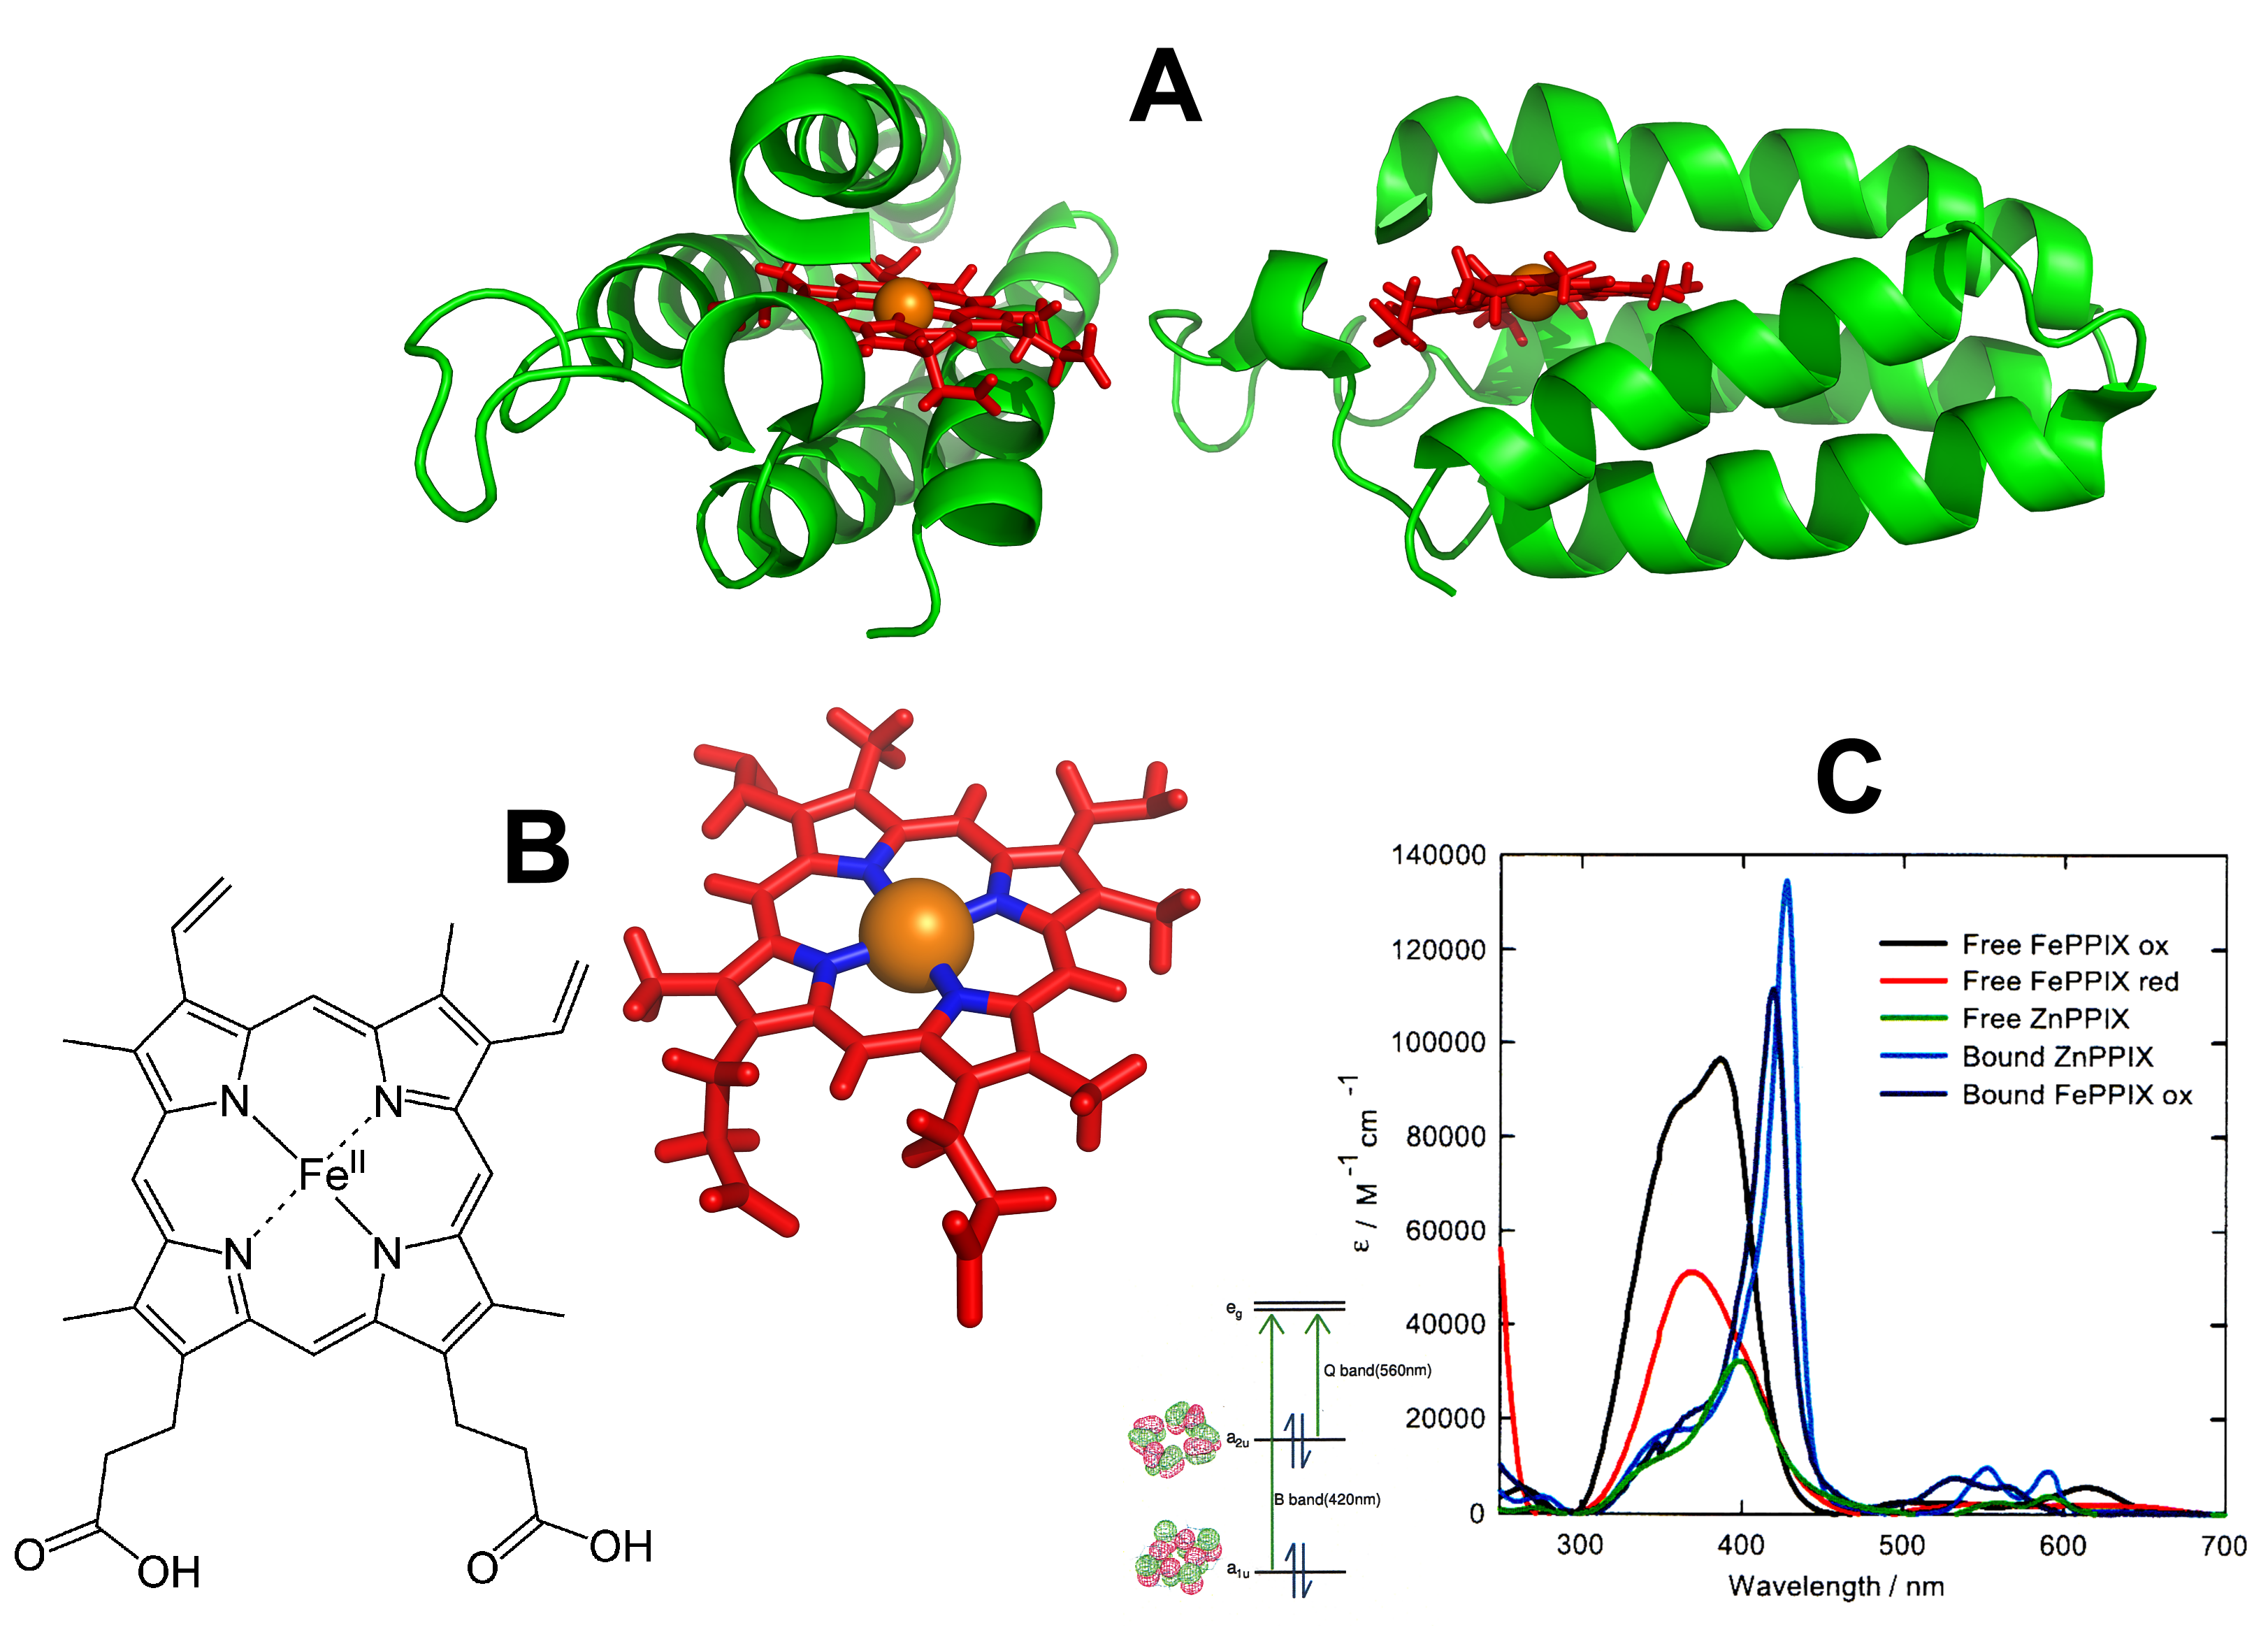
\includegraphics[width=137.4mm]{Images/haemStructure.png}
	\caption[Haem Structure]{A fancy image from Chris' Thesis.}
	\label{fig:haemStructure}
\end{figure}

In this example the command {\textbackslash}includegraphics tells LaTeX to look in the directory `Images' and incorporate the file called `haemStructure.png' into the final document while setting the width to 137.4mm.  This command can be used to resize a graphical file using the height or width parameter as shown. You must specify the units which can be pt, ex, em, mm, cm and so on. LaTeX recognises a very wide variety of standard units and graphics formats. The command is part of the graphicx package and so in the preamble you must include the command {\textbackslash}usepackage\{graphicx\}.

Many packages have been written to provide new commands. For example the `subfigure' package enables you to place separate images or files in the same figure side by side while giving them their own label. However, in this document we only concentrate on the very basics.

\section{Floating Environments}

Both tables and figures are examples of a `floating environments' which means LaTeX decides where to put them. 

The mysterious [!tbh] letters give guidance to LaTeX about roughly where the figure or table is  allowed to be, but in general they can move a long way from where you position them within your text file.  The letters in the square bracket can be t, h or b which stand for top, here or bottom.  If you don't specify any letters LaTeX defaults to [t].

LaTeX will always preserve the order in which figures appear.  If it cannot find a type setting solution, then it may move the float to it's own page, and combine it with other figures. If it still can't fit that in for some reason then it moves the float to the end of the document.  This has the effect of pushing all the remaining floating environments to the end of the document also.

The exclamation mark instructs LaTeX to ``try harder'' at putting the float where you told it to. Often you must play around to ensure the float positioning is acceptable, but usually this can be achieved by stretching or shrinking the image slightly using the size parameter, re-ordering text, judicial applications of the {\textbackslash}pagebreak command or by shouting loudly and slapping the computer monitor about. Note that it is better to resize the image using the original program that was used to create the image. Also using vector graphics can assist be useful (e.g. eps files) because they are designed to scale better.
\chapter{The Chapter on Making Chapters}
\label{sec:Chapters}

Right. LaTeX forces you to structure your document. There a series of simple commands for achieving this:

\vspace*{2ex}

{\textbackslash}chapter\{chapterName\}

{\textbackslash}section\{sectionName\}

{\textbackslash}subsection\{subsectionName\}

{\textbackslash}subsubsection\{subsubsectionName\}

\vspace*{2ex}

Easy enough. At the start of each chapter or section just issue one of these commands to name the section and LaTeX will present the chapter heading in the right style of font, which will be the same style of all the other heading names at that level of hierarchy throughout the document. In addition LaTeX assigns a number to that section. For example, this chapter was created using the command:

\vspace*{2ex}

{\textbackslash}chapter\{The Chapter on Making Chapters\} 

\vspace*{2ex}

LaTeX assigns the correct chapter number to each chapter in turn and then puts it in the table of contents, as you can see by looking at the table of contents! Easy.

\pagebreak
\section{The Section About Sections}
\label{sec:Section}
I think you're getting the hang of this. This section was created using the command {\textbackslash}section\{The Section About Sections\}. It appears in the table of contents as section \ref{sec:Section}.

\subsection{The Sub-Section About Sub-Sections}
\label{sec:SubSection}
Now you're really getting the hang of this. This subsection was created using the command {\textbackslash}subsection\{The Sub-Section About Sub-Sections\}. 

\subsubsection{The Sub-Sub-Section About Sub-Sub-Sections}
\label{sec:SubSubSection}
Now you're really getting the hang of this. but.. caught you out! This subsubsection doesn't have a number!  Ha Ha! It was created using the command {\textbackslash}subsubsection\{The Sub-Sub-Section About Sub-Sub-Sections\} in the same vein as all the other subsections/chapters etc. Here we have stopped the depth of the section numbering at the second level with the command:

\vspace*{2ex}

{\textbackslash}setcounter\{secnumdepth\}\{2\}

\vspace*{2ex}

Easy. WYSIWYM.  LaTeX does what you tell it to do. This is both a blessing and a curse.

\pagebreak
\section*{The Section About Sections That Don't Appear in the Table of Contents}
\label{sec:InvisibleSection}
Ok. Now we're throwing a spanner in the works. This section was created using the command:

\vspace*{2ex}

{\textbackslash}section*\{The Section About Sections That Don't Appear in the Table of Contents\}. 

\vspace*{2ex}

Notice how LaTeX has not assigned a number to the section and it doesn't appear in the table of contents. The effect of the * is to suppress the inclusion of a chapter, section or subsection in the automatic numbering. Easy. You can do this at any level. This is useful for things like prefaces, tables of contents or acknowledgements which you may or may not wish to have an entry in the main contents table. Up to you. It's your thesis. Don't just copy me.

\section{A Small Point About Numbering}

In this section notice how the numbering starts from where it left off before we suppressed the numbering on the previous section. Easy. WYSIWYM.
\pagebreak
\section{The Section About Internal Referencing}
\label{sec:InternalReferencing}

There are two related commands:

\vspace*{2ex}

{\textbackslash}label\{labelName\} 

{\textbackslash}ref\{labelName\}

\vspace*{2ex}


The {\textbackslash}label\{\} command allows you to create a label in a particular environment\footnote{That's right. Chapters, Sections and sub-sections etc are environments!}. The label won't appear in the final document. It's just a label which makes it easy to refer back to any particular environment elsewhere in the document. The {\textbackslash}ref\{\} command enables you to insert a reference anywhere in the document to any label in the document.  For example this is section \ref{sec:InternalReferencing}. The names you use in a label can be anything you like but musn't contain whitespace or special characters. I used the two commands:

\vspace*{2ex}

{\textbackslash}label\{sec:InternalReferencing\}

{\textbackslash}ref\{sec:InternalReferencing\}.

\vspace*{2ex}

The astute among you will realise that LaTeX has to read the document several times. Once to find the labels and then again to populate the references with the correct numbers. So you have to compile a latex document twice to get the referencing right. If there is a missing label or you refer to something that doesn't exist then latex inserts a convenient ? at that point. So hunting for queries is useful way of finding broken references. Latex issues warnings when it finds broken references.

As you create a document you will find yourself putting labels in all over the place so choose a sensible naming convention to help you remember the label names.

Each type of environment (equations, figures, tables, sections etc) has its own independent numbering system.  So when you choose your label name it's a good idea to have an identifier for that type of environment.  I have my own convention for label names which I use to help me remember references. E.g.   sec:SectionAboutCats. Eqn:EquationAboutCats,  Fig:FigureAboutCats and so on. This means you can differentiate between referring to the section or the figure more easily, even though they are about the same thing.

So Internal Referencing is a doddle. Easy!
\chapter{External Referencing}

Referencing is usually performed using a separate program called BibTex.  This program understands the file format .bib.

To create a reference within your document first you must create a .bib file by exporting your list of references from which ever referencing software you used, such as endnote, mendeley or whatever you use.

You can refer to an entry in the .bib file using the {\textbackslash}cite\{ref:Name\} command. the identifier `ref:Name' is the unique identifier which is the first line of each item included in your bibliography file.

For example, open the file LaTexCourseBib.bib in the bibliography directory. The first entry has the identifier `Horcas2007'.  This can be invoked as follows:


\begin{verbatim}
For example, this interesting fact\cite{Horcas2007}, is a cracking example.
\end{verbatim}

For example, this interesting fact\cite{Horcas2007}, is a cracking example.

During compilation latex and bibtex co-operate. During the first compilation latex generates a list of references that it needs.  During the second compilation bibtex populates the details from the .bib file into a shorter, ordered .bib file. The third compilation inserts markers at the right place in the main file and the fourth compilation generates the final list of references. Thus the compilation sequence is latex, bibtex, latex, latex.

The style of the referencing format can be changed using the command {\textbackslash}bibliographyStyle\{\}. e.g. the style used in this document is cjfthesisv1.bst which is invoked by 

\begin{verbatim}
\bibliographystyle{Bibliography/cjfthesisv1}
\end{verbatim}

The location of the list of references in the document is specified by issuing the {\textbackslash}bibliography\{\} command which also specifies the master bibliography file.

\begin{verbatim}
\bibliography{Bibliography/LaTeXCourseBib}
\end{verbatim}




\chapter{Organising Your Files}
One of the drawbacks of word is that the figures and tables are included within the document which becomes very very clunky quite quickly and once it reaches around 100Mb it becomes unwieldy and hard to export. One of that advantages of LaTeX is that the files are all text files and so are very light on resources and are easy to email around the place.

However, sometimes it can be difficult to navigate through a single text file, so if you had a huge document then it becomes difficult to find your way around.  One way of circumnavigating this problem is to break the file up into smaller files. As long as LaTeX knows where to look you can have a file for each logical sub-division of your document.

Therefore it is worth spending a bit of time at the beginning of a large project deciding how you wish to break up your LaTex Files and organise them neatly and tidily.  You can then tell LaTex where to look for the files using the following command:

\vspace*{2ex}
{\textbackslash}include\{fileName\}
\vspace*{2ex}

\pagebreak
\section{Linking a File}
We are now going to copy part of the tutorial file into a separate files and link it the main file.  Because this could go wrong it is sensible to back up tutorial.tex as something else. So save a copy called `tutorialOriginal.tex' for safe keeping. Then follow the following instructions.

\begin{enumerate}
\item Create a new file called MyFirstPage.tex
\item Select and Cut out the first chapter of Tutorial.Tex
\item Paste the first chapter into MyFirstPage.tex
\item Save both tutorial.tex and MyFirstPage.tex
\item Then add {\textbackslash}include\{MyFirstPage\} in tutorial.tex where the text used to be before you cut it out. We don't need to add the `.tex' because LaTeX can only include `.tex' files.
\item compile tutorial.tex and view the PDF
\end{enumerate}

The final PDF should look exactly the same as it was! except we now have a separate file for one of the chapters.

\pagebreak
\section{Creating A Class File}
We can also save our preamble in a separate file called a class file. This makes your main document much easier to understand.  To make it work we need to use the {\textbackslash}LoadClass\{\} command as follows: 

\begin{enumerate}
\item Create another new file and save it as TutorialStyle.cls
\item Copy the preamble of tutorial.tex into the new file. Starting with the {\textbackslash}documentclass{} command and copy right up to, but not including, the {\textbackslash}begin{document} command. Delete the preamble in the original document.
\item Save TutorialStyle.cls and tutorial.tex
\item Modify the first line of TutorialStyle.cls by replacing the word `document' with the word `Load'.
\item Add a new first line of tutorial.tex to use your new style class {\textbackslash}documentclass\{TutorialStyle\}
\item Save both files.
\end{enumerate}

\subsection{Sanity Check}

The first line of TutorialStyle.cls should now be:

\begin{verbatim}
\LoadClass[12pt, oneside, a4paper]{book}
\end{verbatim}
\vspace{2ex}

The first line of tutorial.tex should be:

\begin{verbatim}
\documentClass{TutorialStyle}
\end{verbatim}
\vspace{2ex}

We have just created what is called a style file. You can use this style file as a generic preamble for other documents as well. Compile tutorial.tex.  Nothing should have changed in the final PDF.


\pagebreak
\section{The Structure of this Document}

Lets now look at how I've organised this document. It is identical to my thesis because it started out life as my thesis. I usurped the structure and simply replaced the headings and content to make a kind of reference manual for this introductory course. This document therefore is three things:

\begin{enumerate}
\item An example thesis structure to work from.
\item The LaTeX files which were used to create it can be used as a template for a thesis.
\item It is also a convenient introductory latex manual!
\end{enumerate}

\vspace*{2ex}
Groovy huh?

\section{The Master File}

There is a master file where LaTeX begins the compilation procedure. This contains the {\textbackslash}documentclass command needed to set the ball rolling. Within the file there are a series of {\textbackslash}include\{\} commands, one for each Chapter, which tell LaTeX where to find the files containing each chapter.

The subfiles cannot be compiled on their own because they do not contain the {\textbackslash}documentclass, {\textbackslash}begin\{document\} or {\textbackslash}end\{document\} commands. Lets us look in more detail at the master file and we will learn some new LaTeX commands.

\singlespacing
\pagebreak
\begin{verbatim}
\documentclass{Style/LatexCourseStyle}

\begin{document}
\setcounter{secnumdepth}{2}
\setcounter{tocdepth}{1}

\frontmatter
\onehalfspacing
\include{Frontmatter/Titlepage}
\include{Frontmatter/Declaration}
\include{Frontmatter/Acknowledgements}
\include{Frontmatter/Summary}
\include{Frontmatter/Abbreviations}
\tableofcontents
\listoftables
\listoffigures

\mainmatter
\renewcommand{\sectionmark}[1]{\markright{\thesection \ #1}{}}
\include{Chapters/Overview}
\include{Chapters/MyFirstPage}
\include{Chapters/Lists}
\include{Chapters/mathsEquations}
\include{Chapters/ChemicalEquations}
\include{Chapters/Tables}
\include{Chapters/Figures}
\include{Chapters/Sectioning}
\include{Chapters/externalReferencing}
\include{Chapters/ThesisTemplateMainFile}
%\include{Chapters/ChapterThatIsNotCompiled}

\appendix
%\include{Appendices/UsefulWebsites}

\singlespacing

\backmatter
\addcontentsline{toc}{chapter}{References}
\bibliographystyle{Bibliography/cjfthesisv1}
\renewcommand{\bibname}{References}
\bibliography{Bibliography/LatexCourseBib}

\end{document}
\end{verbatim}
\onehalfspacing
\pagebreak

\section{Analysing the Master File}
Let us go through this file and observe the new commands. Most of it is self-explanatory.

\begin{verbatim}
\documentclass{Style/LaTeXCourseStyle}
\end{verbatim}

This command tells latex that the document class is the one defined in the the style file ''LaTeXCourseStyle'', which is in the sub directory ''style''.  Easy.

\begin{verbatim}
\setcounter{secnumdepth}{2}
\setcounter{tocdepth}{1}
\end{verbatim}

The first of these commands tells latex that the section depth number is 2. I.E. throughout the document only bother numbering sections, subsections and subsubsections down to the second level (such as section 1.2.3). The second command tells latex to only build the table of contents from section numbers down to the first level i.e. 1.1.  Easy enough.

The command {\textbackslash}frontmatter is exclusive to the book class, on which this style is based, and tells latex that within this section to number the pages using roman numerals, and not to include these numbers in the table of contents, just like in a book. The {\textbackslash}mainmatter and {\textbackslash}backmatter commands similarly delineate the other sections of the document.  

Childs play.  How long would it take you to figure out how to do that in word???? No idea. I've never tried.

Note that these rather cool commands are not available in every single class. So for a paper you would use the article class where such compartmentalisation of your document is not appropriate. In fact you can often download latex templates from the journal to wish to submit your paper, which is why I concentrate on the thesis template in this course.

\begin{verbatim}
\onehalfspacing
\end{verbatim}

Is obvious. ''From this point forward use line spacing of one and a half lines please. Thank you.'' How many hours have you spent clicking on paragraph indentations for each separate paragraphs in word? Nightmare. Want to change the standard in the whole document? Not a chance in word. In latex, you can do it with a single word, carefully placed in the master file.

\begin{verbatim}
\include{Frontmatter/Titlepage}
\include{Frontmatter/Declaration}
\include{Frontmatter/Acknowledgements}
\include{Frontmatter/Summary}
\include{Frontmatter/Abbreviations}
\end{verbatim}

The {\textbackslash}include\{\} command tells latex to include the specified .tex file at this point.  Thus it is a simple matter to break up a large document into sub components.  I have written each part of the front matter in a separate file and then grouped all the front matter into one directory called: Frontmatter.

See how the directory structure of my files reflects the structure of my book?

\begin{verbatim}
\tableofcontents
\listoftables
\listoffigures
\end{verbatim}

Again. This is easy. These commands mean: ''Please scan through the whole document and build for me a table of contents, a list of tables, a list of figures and then write down the entries along side their section numbers (as I have them ordered in this version of the document), as well as the page numbers on which they appear and create a nice little summary table and add them to the front matter of my document. Thanks.''.

How does latex do this?  remember the idea of environments?  Well each table, figure, equation etc is a defined environment.  LaTeX just counts them up and assigns numbers starting wherever you want and builds a table.  You can tell latex to ignore individual sections if you want to.

You can also control the look and feel of your table of contents with subtley and grace. Do you want to fill the white space with lines of dots to aid readability, even though the chapter titles are all different lengths? page numbers? How deep should the TOC been?  etc etc etc. How to do this is beyond the scope of this course, but now you know about it, go look it up. easy as $\pi$.

Ok.

Main matter we've done.

\begin{verbatim}
\renewcommand{\sectionmark}[1]{\markright{\thesection \ #1}{}}
\end{verbatim}

This command tells latex to 'renewcommand', i.e. change the meaning of the following command from this point in the document forward, over-riding previous definitions.
\begin{verbatim}
\sectionmark}[1]{\markright{\thesection \ #1}{}
\end{verbatim}

Is latex speak for ``please write the section heading at the top right hand side of each page. thanks''. This works in conjunction with a command in the style file which we'll talk about later. You have to tell latex to switch on headings as well as where to put them.

\begin{verbatim}
\include{Chapters/Overview}
\include{Chapters/MyFirstPage}
\include{Chapters/Lists}
\include{Chapters/mathsEquations}
\include{Chapters/ChemicalEquations}
\include{Chapters/Tables}
\include{Chapters/Figures}
\include{Chapters/Sectioning}
\include{Chapters/externalReferencing}
\include{Chapters/ThesisTemplateMainFile}
%\include{Chapters/ChapterThatIsNotCompiled}
\end{verbatim}

This is the include command again. You will notice that one of the include lines is commented out. This is a handy trick to only build certain parts of my thesis. Which can be useful if individual chapters are being reviewed.

\pagebreak

\begin{verbatim}
\appendix
%\include{Appendices/UsefulWebsites}

\singlespacing

\backmatter
\addcontentsline{toc}{chapter}{References}
\bibliographystyle{Bibliography/cjfthesisv1}
\renewcommand{\bibname}{References}
\bibliography{Bibliography/LatexCourseBib}
\end{verbatim}

The rest is easy. {\textbackslash}Appendix means we are in the appendix now and start labelling sections with A.1.2 instead of 1.2.3.  

{\textbackslash}addcontentsline means forcibly insert a contents line about the references into the contents table. 

{\textbackslash}\{bibliographystyle\{Bibliography/cjfthesisv1\}\} means use the biblography style defined in the file cjfthesisv1. Defining a bibliography style will be covered later if we have time. This is where you specify how the references will appear (names, journals, full stops, commas etc).

{\textbackslash}renewcommand\{{\textbackslash}bibname\}\{References\} means: rename the bibliography chapter as `References'

{\textbackslash}biblography means add the following bibliography.  You can reference entries in this bibliography file very easily.

The astute among you will realise that LaTeX will have to read the document several times before it can be compiled with all the references.  Hey ho. No problem. You can go and have a cuppa while LaTeX does your references for you in the style of your favorite journal... nice.




%\include{Chapters/ChapterThatIsNotCompiled}

\appendix
%\include{Appendices/UsefulWebsites}

\singlespacing

\backmatter
\addcontentsline{toc}{chapter}{References}
\bibliographystyle{Bibliography/cjfthesisv1}
\renewcommand{\bibname}{References}
\bibliography{Bibliography/LatexCourseBib}

\end{document}
\end{verbatim}
\onehalfspacing
\pagebreak

\section{Analysing the Master File}
Let us go through this file and observe the new commands. Most of it is self-explanatory.

\begin{verbatim}
\documentclass{Style/LaTeXCourseStyle}
\end{verbatim}

This command tells latex that the document class is the one defined in the the style file ''LaTeXCourseStyle'', which is in the sub directory ''style''.  Easy.

\begin{verbatim}
\setcounter{secnumdepth}{2}
\setcounter{tocdepth}{1}
\end{verbatim}

The first of these commands tells latex that the section depth number is 2. I.E. throughout the document only bother numbering sections, subsections and subsubsections down to the second level (such as section 1.2.3). The second command tells latex to only build the table of contents from section numbers down to the first level i.e. 1.1.  Easy enough.

The command {\textbackslash}frontmatter is exclusive to the book class, on which this style is based, and tells latex that within this section to number the pages using roman numerals, and not to include these numbers in the table of contents, just like in a book. The {\textbackslash}mainmatter and {\textbackslash}backmatter commands similarly delineate the other sections of the document.  

Childs play.  How long would it take you to figure out how to do that in word???? No idea. I've never tried.

Note that these rather cool commands are not available in every single class. So for a paper you would use the article class where such compartmentalisation of your document is not appropriate. In fact you can often download latex templates from the journal to wish to submit your paper, which is why I concentrate on the thesis template in this course.

\begin{verbatim}
\onehalfspacing
\end{verbatim}

Is obvious. ''From this point forward use line spacing of one and a half lines please. Thank you.'' How many hours have you spent clicking on paragraph indentations for each separate paragraphs in word? Nightmare. Want to change the standard in the whole document? Not a chance in word. In latex, you can do it with a single word, carefully placed in the master file.

\begin{verbatim}
\thispagestyle{empty}

\begin{center}
\vspace*{\stretch{1}}

\hrule height 2pt
\vspace*{2ex}
{\Huge\textbf{Towards the Ability to Make Super Duper LaTeX Documents}\par}
\vspace*{2ex}
\hrule height 2pt
\vspace*{10ex}
{
\includegraphics[height=40mm]{Images/UnivShield}\par}
\vspace*{10ex}
{\large\textbf{Christopher~James~Forman}\par}
\vspace*{2ex}
{\large{Department Of Chemistry}\par}
\vspace*{2ex}
{\large{University of Cambridge}\par}
\vspace*{5ex}
{\large{This dissertation is submitted for the degree of \textit{Doctor of Philosophy}}\par}
\vspace*{5ex}
{\large{\today}\par}

\vspace*{\stretch{2}}
\end{center}
\chapter*{Declaration}

\vfill

This dissertation is the result of my own work and includes nothing which is the outcome of work done in collaboration except where specifically indicated in the text. It is not substantially the same as any that I have submitted for a degree or diploma or other qualification at any other University and no part has already been, or is concurrently being, submitted for any degree, diploma, or other qualification. It does not exceed 60,000 words, including tables, footnotes, bibliography and appendices.\par

\vspace{10ex}

\begin{flushright}
Signature: \rule[0pt]{60mm}{0.5pt}

\vspace{5ex}

Date: \rule[0pt]{60mm}{0.5pt}
\end{flushright}

\vfill
\chapter*{Acknowledgments}
\subsection*{Family}
Mum. Dad. Pet Dog.

\subsection*{Scientific Collaborations}
Dr A.N.Other at uni of blah for samples and instrument time etc. My Amazing Lab Chums.

\subsection*{Scientific Support}
My amazing lab chums.

\subsection*{General Assistance}
Cleaner, My amazing lab chums.

\subsection*{Financial Support}
Bank, Tax payer. My amazing lab chums.

\subsection*{Moral Support}
My Amazing Lab chums.

\subsection*{Academic Inspiration}
Netwon, My super. My Amazing Lab Chums.

\subsection*{Everyone else}
My Amazing Lab Chums.

\chapter*{Summary}
This document is a handbook for introducing you to LaTeX. It contains a bit of background about the history and philosophy of LaTeX.  However, it concentrates on providing a guided practical introduction to the basic techniques such as 
\begin{itemize}
\item Lists
\item Mathematical and chemical equations
\item Tables
\item Figures
\item Chapters and Sections
\item Linking to other files in large documents
\item Referencing
\end{itemize}

The handbook is also presented in the style of a thesis. This means that source files provided on the introductory course and available from the department web page are a convenient template for a thesis.

More details on specific aspects of LaTeX can be found at the departmental LaTeX page which can be found here:

 http://www-ch-int.ch.private.cam.ac.uk/latex/about

\chapter*{Abbreviations}

\begin{longtable}{r >{\rule{0pt}{3ex}}l<{\rule[-1.5ex]{0pt}{0pt}}}
ADP & Adenosine Diphosphate\\
(nc/c)AFM & (non-contact/conducting) Atomic Force Microscopy\\
ATP & Adenosine Triphosphate \\
\end{longtable}
\end{verbatim}

The {\textbackslash}include\{\} command tells latex to include the specified .tex file at this point.  Thus it is a simple matter to break up a large document into sub components.  I have written each part of the front matter in a separate file and then grouped all the front matter into one directory called: Frontmatter.

See how the directory structure of my files reflects the structure of my book?

\begin{verbatim}
\tableofcontents
\listoftables
\listoffigures
\end{verbatim}

Again. This is easy. These commands mean: ''Please scan through the whole document and build for me a table of contents, a list of tables, a list of figures and then write down the entries along side their section numbers (as I have them ordered in this version of the document), as well as the page numbers on which they appear and create a nice little summary table and add them to the front matter of my document. Thanks.''.

How does latex do this?  remember the idea of environments?  Well each table, figure, equation etc is a defined environment.  LaTeX just counts them up and assigns numbers starting wherever you want and builds a table.  You can tell latex to ignore individual sections if you want to.

You can also control the look and feel of your table of contents with subtley and grace. Do you want to fill the white space with lines of dots to aid readability, even though the chapter titles are all different lengths? page numbers? How deep should the TOC been?  etc etc etc. How to do this is beyond the scope of this course, but now you know about it, go look it up. easy as $\pi$.

Ok.

Main matter we've done.

\begin{verbatim}
\renewcommand{\sectionmark}[1]{\markright{\thesection \ #1}{}}
\end{verbatim}

This command tells latex to 'renewcommand', i.e. change the meaning of the following command from this point in the document forward, over-riding previous definitions.
\begin{verbatim}
\sectionmark}[1]{\markright{\thesection \ #1}{}
\end{verbatim}

Is latex speak for ``please write the section heading at the top right hand side of each page. thanks''. This works in conjunction with a command in the style file which we'll talk about later. You have to tell latex to switch on headings as well as where to put them.

\begin{verbatim}
\chapter{Overview}
\label{chap:overview}
\section{LaTeX: The answer to everything.}
LaTeX is typsetting program that takes an input file of marked up text and then, with a user defined set of rules, typesets a beautifully crafted output file that can be easily printed (e.g. a pdf). 

\subsection{Advantages}

The advantages of this method are manifold:

\begin{itemize}

\item Use any text editor to view the source document.
\item More time can be spent working on the content and not worrying about how text or figures interact in the layout until later on.
\item LaTeX uses consistent rules throughout a document
\item LaTeX sorts out basic typesetting automatically
\item Changes can be introduced globally with very little effort
\item Document structure is explicit
\item Documents can be professionally typeset and look great
\item You are forced to structure your documents correctly.
\item Mathematical equations, like $E=mc^2$ or $\imath\hbar\frac{\partial}{\partial t}\Phi (x, t) = \hat{H}\Phi (x, t)$ can be produced almost as fast as typing (if you know the commands!).
\end{itemize}

\subsection{Disadvantages}
The disadvanatges of this method are also manifold:
\begin{itemize}
\item You don't see the output as you go.
\item Steep learning curve.
\item Documents are harder to edit by a second author (unless they are adept at LaTeX too). This can be mitigated using version control, which makes group authoring processes superior to word.
\item The program never works quite the way you want it to and learning how to influence it can be problematic and subtle.
\item Although intended to save work the principle of 'conservation of work' means that you simply transform problems associated with WYSISYG approaches to problems associated with WYSIWYM approaches!
\item You can go blind trying to determine the difference between wiggly and smooth brackets if your editors font isn't large enough.
\end{itemize}

\subsection{On balance?}
If it's so rubbish, why use LaTeX?

\begin{itemize}
\item Large documents are much more easily handled. 
\item In general it is quicker to debug a LaTeX document than typeset an entire thesis manually. 
\item Technical information such as tables, equations and figures are integrated much more smoothly than with word.
\end{itemize}

\section{How does it work?}

The raw text is interspersed with commands, preceded by a \textbackslash, which tell LaTeX what to do with the text. For example you can \textbf{make it bold}, \emph{italic}, or \underline{underlined} with the commands {\textbackslash}textbf\{\}, {\textbackslash}emph\{\} or {\textbackslash}underlined\{\}. More on commands in a moment...



\chapter{My First Page}

\section{The Very Beginning}
The very simplest LaTeX document might look like this:

\begin{verbatim}
\documentclass[a4paper,12pt]{article}
\begin{document}
Hello World.
\end{document}
\end{verbatim}

\pagebreak
\thispagestyle{empty}
Hello World.
\pagebreak
\subsection{Break Down}
What's all the gobbledegook around my simple message???

In LaTeX we intersperse text and commands.  Commands are preceded by a \textbackslash. For example the first line in a LaTeX document \underline{\textbf{\emph{must}}} be:

\begin{verbatim}
\documentclass[options]{class}
\end{verbatim}

Where the word ''class'' may be substituted for one of many things such as: article, proc, minimal, report, book, letter, memoir, slides, beamer.

Similarly, and completely generally in LaTeX speak, the square brackets denote the existence of optional parameters. Each individual command can take its own parameters and for the ''{\textbackslash}documentclass'' command there are options for controlling font size, font family, landscape, oneside, twosided, page size and so on. These options will persist throughout the entire document. For example the document class command for this document, (which is likely to be like the one you would use for a thesis), would be:

\begin{verbatim}
\documentclass[12pt, oneside, a4paper]{book}
\end{verbatim}

Other options include:

\begin{itemize}
\item {10pt, 11pt, 12pt (default is 10pt).}
\item {letterpaper, legalpaper, a4paper, executivepaper, a5paper, b5paper}
\end{itemize}
and so on.

\pagebreak
\section{Can I start typing please?}

After we have set up the document we can start actual work on our document. So we must tell LaTeX that what follows is to be interpreted as a document.  The command {\textbackslash}begin can take many different parameters and is a command to enter what is known, in LaTeX speak, as 'an environment'. Thus the commands:
\begin{verbatim}
\begin{document}

\end{document}
\end{verbatim}

tells LaTeX to enter and leave the document environment, and thus constitute the outer limits of our document file. Other environments include the equation environment, the itemize environment, the figure environment and so on. These will be encountered in due course.

Every part of the LaTeX file is therefore within an environment of specific type and the content within each environment consists of commands or text.

That's basically it.

So let's get on with it shall we...

\pagebreak
\section{The ground rules}
\begin{quote}
Hold on, hold on, hold on my son.

First the lessons.

Then the fun!
\end{quote}
Dr Seuss.

\subsection{Spaces}
Whitespace characters, such as blank or tab, are treated uniformly as space by LaTeX. Several consecutive whitespace characters are treated as one single space. Whitespace at the start of a line is generally ignored, and a single line break is treated as whitespace. An empty line between two lines of text defines the end of a paragraph. Several empty lines are treated the same as one empty line. The text below is an example.

\begin{verbatim}
It does not matter whether you
enter one or several             spaces
after a word. The final result will be typeset beautifully
according    to     precise rules.




An empty line starts a new
paragraph. Note the indentation on the first line of the paragraph, 
except at the beginning of the section. 
\end{verbatim}

\vspace*{2ex}
\vspace*{2ex}

It does not matter whether you
enter one or several             spaces
after a word. The final result will be typeset beautifully
according    to     specific rules.




An empty line starts a new
paragraph. Note the indentation on the first line of the paragraph, except at the beginning of the section. 

\pagebreak
\subsection{Special Characters}
The symbols 

\# \$ \% \textasciicircum{} \& \_ \{ \} \~{} \textbackslash

are reserved characters that either have a special meaning under LaTeX or are unavailable in all the fonts. If you enter them directly in your text, they will normally not print, but rather make LaTeX do strange things.

To overide the special meanings of these symbols and allow them to produced within your text you may use the following sequences:
\begin{verbatim}
\# \$ \% \textasciicircum{} \& \_ \{ \} \~{} \textbackslash
\end{verbatim}

Other symbols and many more can be printed with special commands in mathematical formulae or as accents.

The backslash character '\textbackslash' cannot be entered by adding another backslash in front of it ( \textbackslash\textbackslash); because this sequence means ''linebreak''.

The command \textbackslash\~{}\{\} produces a tilde which is placed over the next letter. For example \textbackslash\~{}\{n\} gives \~{n}. To produce just the character \~{}, use \textbackslash\~{}\{\} which places a \~{} over an empty box.

Similarly, the command \textbackslash\textasciicircum{} produces a hat over the next character, for example \textbackslash\textasciicircum\{o\} produces \^{o}.

\pagebreak
\section{Preamble}
After the {\textbackslash}documentclass command we add ''preamble''. Here we load special features that we will use throughout our document to expand on the basic capabilities of LaTex. These are contained in units called ''packages'' which we can tell our LaTeX compiler to download by using the command ''{\textbackslash}include\{packageName\}''. 

There are many repositories of such packages on the web. Your compiler generally knows where to look and most standard packages are included with any install. For example, to include a special set of typesetting instructions to handle chemical equations we can grow our simple document with a single command like this:

\begin{verbatim}
\documentclass[a4paper,12pt]{article}
\usepackage[version=3]{mhchem}
\begin{document}
Hello World!

We all need \ce{H2O}.

I'm less fussed about \ce{^{235}_{92}U+}.

\end{document}
\end{verbatim}

\vspace{2ex}

\pagebreak
\thispagestyle{empty}
Hello World!

We all need \ce{H2O}.

I'm less fussed about \ce{^{235}_{92}U+}.
\pagebreak

Here we have loaded a package called: "`mhchem"' which took the option ''[version=3]''. This is a package for drawing chemical equations easily and it has it's own instruction manual which you can follow easily. It is included in the bundle of files for this course.

Other things we can do in the premable within LaTeX are to redefine existing commands or create our own personal commands. These can be stored in a file called the 'style file' which we can load at the beginning of our document, in place of our documentclass. More about this later on...


\subsection{Comments}
It is often useful to comment your LaTeX documents. You can leave yourself amusing, sarcastic messages that won't get printed out in the final document. Use this to make your own notes as the course progresses.

To get a comment use the \% command, which tells LaTeX to ignore the rest of the line, the line break and all the white space at the beginning of the next line, for example, we may add to our continually evolving document...

\begin{verbatim}
\documentclass[a4paper,12pt]{article}
\usepackage[version=3]{mhchem}
\begin{document}
Hello World!

%All humans need water and I would like 
%to include this concept in my arguments.
We all need \ce{H2O}.

%Uranium 235 is toxic, which is why I don't want to consume it... 
I'm less fussed about \ce{^{235}_{92}U+}.

\end{document}
\end{verbatim}

\vspace{4ex}
Hello World!

%All humans need water and I would like to include this concept in my arguments.
We all need \ce{H2O}.

%Uranium 235 is toxic, which is why I don't want to consume it... 
I'm less fussed about \ce{^{235}_{92}U+}.

\pagebreak
\section{Compiling}
Once the document is finished you can compile it. Your compiler will depend on the platform that you use. In the PWF we are using winEDT to edit the documents (a LaTeX front end) and texlive2008 which is the compiler itself. I use MiKTex and the front end texCenter.  There is no need to use a front end. If you prefer you can use a simple text editor and a command line.

the recommended distributions are:
\begin{itemize}
\item MiKTeX or TeX Live for Windows
\item TeX Live for Unix/Linux
\item MacTeX or TeX Live for Mac OS.
\end{itemize}

Once you have installed your software and got it working, written your source code and tried to compile it, there will nearly always be something wrong with your file. 

Any errors will be highlighted in the console window or error output box of your front end.  Some front ends dump the running commentary which LaTeX produces into a text file for easy reading afterwards.

In a compile attempt (successful or otherwise) LaTeX may produce the following files:

projectname.aux

projectname.bbl

projectname.lof

projectname.lot

projectname.txt

projectname.toc

projectname.dvi

These are interim files (toc= table of contents, bbl = bibliography etc). To be honest I have no idea what half of these things contain.  You only need the .tex file and a compiler with the right packages installed to produce them again.

Some versions of LaTeX only produce DVI files and you then need to convert the dvi file to a PDF or download a dvi viewer. You can also convert DVI files to PS files and then view them.  The good thing about front ends is that you can set them up to produce PDFs directly.

OK. So we have now produced a silly document but we understand it.  Now lets get on with learning how to make our own documents.



\chapter{Lists}
Lists are great.  The command {\textbackslash}begin\{\} can be used to enter a list environment.  For example:

\begin{verbatim}
\begin{itemize}
\item cat
\item dog
\item horse
\end{itemize}
\end{verbatim}

Produces:

\begin{itemize}
\item cat
\item dog
\item horse
\end{itemize}

\pagebreak
We can also replace the bullet points with numbers using the enumerate keyword.

\begin{verbatim}
\begin{enumerate}
\item cat
\item dog
\item horse
\end{enumerate}
\end{verbatim}

\begin{enumerate}
\item cat
\item dog
\item horse
\end{enumerate}

\pagebreak
and we can use the description keyword which does this:
\begin{verbatim}
\begin{description}
\item[Cat] a lovely furry creature with a cute nose and whiskers.
\item[Dog] Another furry creature that smells rather well; 
           its olfactory power stems from its nasal dampness.
\item [Horse] A large stinky creature with sideways facing eyes.
\end{description}
\end{verbatim}

\begin{description}
\item[Cat] a lovely furry creature with a cute nose and whiskers.
\item[Dog] Another furry creature that smells rather well; its olfactory power stems from its nasal dampness.
\item [Horse] A large stinky creature with sideways facing eyes.
\end{description}
\chapter{Maths Equations}

\section{Producing Beautiful Looking Mathematics}

One of the best features about LaTeX is `maths mode'.  For example the schrodinger equation can be produced as follows:

\vspace*{2ex}

\begin{center}
\begin{math}
\imath\hbar\frac{\partial}{\partial t}\Phi (x, t) = \hat{H}\Phi (x, t)
\end{math}
\end{center}

\vspace*{2ex}

\begin{verbatim}
\begin{math}
\imath\hbar\frac{\partial}{\partial t}\Phi(x,t)=\hat{H}\Phi(x,t)
\end{math}
\end{verbatim}

There are a number of ways to switch on maths mode.  The first, as above, is with the {\textbackslash}begin\{math\} environment. You can also enter mathmode inline using the \$ symbol. For example typing in \$y=ax\textasciicircum{}2+bx+c\$ yields $y=ax^2+bx+c$.  Another way is to enter the equation environment which enables you to number equations so you can then refer to them later in the text.

\begin{equation}
y(t)= \sin \left(\frac{{\alpha}t}{2\pi} + \phi_0\right)
\label{eqn:MadeUpNonsense}
\end{equation}

\vspace*{2ex}
\begin{verbatim}
\begin{equation}
y(t)= \sin \left(\frac{{\alpha}t}{2\pi} + \phi_0\right)
\end{equation}
\end{verbatim}.

\section{Basic Maths Mode}
Once in maths mode there is a kind of text based code for writing down your equations.  Here are the most basic symbols to get you going.
\begin{center}
\begin{tabular}{cc}
\toprule
Final Result & LaTeX Code \\
\cmidrule(){1-2}
$a+b$ & a+b \\
$a-b$ & a-b \\
$ab$ & ab \\
$a*b$ & a*b \\
$a \times b$ & a {\textbackslash}times b \\
$a \cdot b$ & a {\textbackslash}cdot b \\
$\frac{a}{b}$ & {\textbackslash}frac\{a\}\{b\} \\ 
$a^b$ & a\textasciicircum{}b \\
$a_b$ & a\_b \\
$\sin a$ & {\textbackslash}sin a  (same for cos, tan)\\
$ sin a$ & sin a \\
$\sqrt{a}$ & {\textbackslash}sqrt\{a\} \\
$\left( a \right) $ & {\textbackslash}left( a {\textbackslash}right)\\ 
$\left[ a \right]$ & {\textbackslash}left[ a {\textbackslash}right]\\ 
$\alpha$ & {\textbackslash}alpha \\
$\pi$ & {\textbackslash}pi \\
\bottomrule
\end{tabular}
\end{center}

A full treatise on maths mode is not practical here. There are lots of online tutorials and summaries of symbols. It just takes a bit of practice and you can build up equations really easily. It's straight forward to learn new stuff once you've done it a few times.

\pagebreak
\section{Equation Arrays}
Sometimes you need to arrange several equations vertically, referencing individual lines separately and aligning the equations on the $=$ sign. This can be achieved with equation arrays as follows:

\begin{eqnarray}
A\left( x\right) & = & \frac{x^2+2x+1}{x+1} \\
& = & \frac{\left(x+1\right)\left(x+1\right)}{x+1} \nonumber\\
& = & x+1 \nonumber\\
B(x,t) & = & \frac{e^{\left(\imath\omega_0 t + kx\right)}}{4\pi\epsilon_0}
\end{eqnarray}

\begin{verbatim}
\begin{eqnarray}
A\left( x\right) & = & \frac{x^2+2x+1}{1+x} \\
& = & \frac{\left(x+1\right)\left(x+1\right)}{1+x} \nonumber\\
& = & x+1 \nonumber\\
B(x,t) & = & \frac{e^{\left(\imath\omega_0 t + kx\right)}}{4\pi\epsilon_0}
\end{eqnarray}
\end{verbatim}

\begin{itemize}
\item Note the \& symbols. This tells LaTeX where to align the equations. There must be the same number of \& symbols in each line.
\item Note the \textbackslash\textbackslash ~at the end of each line except the last one. This symbol tells LaTeX to add another row in the array.  If you put it on the last line you get an empty row at the bottom of the array.
\item Note the {\textbackslash}nonumber command which suppresses line numbering for that line.
\item Note that equation number carries on from equation \ref{eqn:MadeUpNonsense} in the previous section.
\end{itemize}

\section{Maths Packages}

Maths mode comes as standard in LaTeX, however you can download packages that buff up your maths symbol set. For example neat vector notation comes in the package `vector'. e.g. {\textbackslash}uuvec\{T\} yields $\uuvec{T}$.

\begin{verbatim}
\usepackage{amssymb}
\usepackage{amsmath}
\usepackage{vector}
\end{verbatim}


\chapter{Chemical Equations}
The mhchem package means you can do basic stuff very easily using {\textbackslash}ce\{\}. For example:

\vspace{2ex}
\begin{verbatim}
\ce{CO2 + C -> 2CO}
\ce{CO2 + C <- 2CO}
\ce{CO2 + C <=> 2CO}
\ce{A-B=C#D\sbond E\dbond F\tbond G}
\end{verbatim}
\vspace{2ex}
\begin{center}
\ce{CO2 + C -> 2CO}

\ce{CO2 + C <- 2CO}

\ce{CO2 + C <=> 2CO}

\ce{A-B=C#D\sbond E\dbond F\tbond G}
\end{center}

\vspace{2ex}
You can also use math mode within chemical equations.
\vspace{2ex}

\begin{center}
\ce{$x\,$ Na(NH4)HPO4 ->[\Delta] (NaPO3)_{$x$} + $x\,$ NH3 ^ + $x\,$ H2O}
\end{center}

\begin{verbatim}
\ce{$x\,$ Na(NH4)HPO4 ->[\Delta](NaPO3)_{$x$} + $x\,$ NH3 ^ + $x\,$ H2O}
\end{verbatim}

And you can number chemical reactions as well by using the math mode equation environment.

\begin{equation}
\ce{CO2 + C <=> 2CO}
\end{equation}

\begin{verbatim}
\begin{equation}
\ce{CO2 + C <=> 2CO}
\end{equation}
\end{verbatim}

However, this will number mathematical and chemical equations using the same number system. There is a discussion in the mhchem pdf which shows you how to number chemical and mathematical equations independently. It's a bit complex and involves you creating your own type of environment... bit beyond the intro level of this course...
\chapter{Tables}
Tables are big business in Latex.  I use these packages to help me.

\begin{verbatim}
\usepackage{multirow}
\usepackage{booktabs}
\usepackage{dcolumn}
\end{verbatim}

Here's an example table

\begin{table}[!hb]
 \centering
	\begin{tabular}{@{}rccc@{~}r@{.}l*3{r@{.}l@{~}r@{.}l}D{.}{\cdot}{2,1}}
	\toprule
	\multicolumn{1}{c}{Fibre Type}
	& N 
	& M 
	&\multicolumn{3}{c}{$L_t$ (nm)}
	&\multicolumn{4}{c}{$R_t$ (nm)}
	&\multicolumn{4}{c}{$d_t$ (nm)}
	&\multicolumn{4}{c}{${\Delta}Z_t$ (nm)}
	&\multicolumn{1}{c}{~}\\
\cmidrule(lr){1-1}
\cmidrule(lr){2-2}
\cmidrule(lr){3-3}
\cmidrule(lr){4-6}
\cmidrule(lr){7-10}
\cmidrule(lr){11-14}
\cmidrule(lr){15-18}
  SS Twisted & 5 & 4 & 313 &\multicolumn{2}{c}{(122)} & 5&7 &(1&6)  & 5&4 &(1&0)  &  150&5 &(63&1) &\multicolumn{1}{c}{~} \\
  \multicolumn{19}{c}{~}\\
  %\cmidrule(lr){3-18}
  &
  &
 	&\multicolumn{3}{c}{$L_s$ (nm)} 
 	&\multicolumn{4}{c}{$R_s$ (nm)}
 	&\multicolumn{4}{c}{$W_s$ (nm)}
 	&\multicolumn{4}{c}{${\Delta}Z_s$ (nm)}
 	&\multicolumn{1}{c}{${\Delta}Z_{e}$ (nm)}\\
\cmidrule(lr){4-6}
\cmidrule(lr){7-10}
\cmidrule(lr){11-14}
\cmidrule(lr){15-18}
\cmidrule(lr){19-19}
  SS Spiral& 32 & 7 &123&(31&6)&11&4&(3&3)&11&1&(2&6)&32&9&(22&2)&26.9\\
  SSB Spiral& 64&18 &106&(22&9)&10&8&(2&7)&9&8&(1&8)&28&2&(8&1)&22.7\\
	%\midrule
  BSS Spiral&37 &19 &110&(44&9)&13&4&(3&0)&12&9&(1&8)&27&1&(9&1)&21.5\\
	%\midrule
  SSSB Spiral&26& 6 &104&(23&9)&13&3&(2&6)&16&4&(3&4)&29&9&(11&1)&22.5\\
	\bottomrule
	\end{tabular}	
	\caption[Basic Fibre Dimensions by TEM]{A funky table from my thesis.}
	\label{tab:BasicXSBFibreDimensionsTEM}
\end{table}

\pagebreak
Here's what the code looks like:
\begin{verbatim}
\begin{table}[!hb]
 \centering
	\begin{tabular}{@{}rccc@{~}r@{.}l*3{r@{.}l@{~}r@{.}l}D{.}{\cdot}{2,1}}
	\toprule
	\multicolumn{1}{c}{Fibre Type}
	& N 
	& M 
	&\multicolumn{3}{c}{$L_t$ (nm)}
	&\multicolumn{4}{c}{$R_t$ (nm)}
	&\multicolumn{4}{c}{$d_t$ (nm)}
	&\multicolumn{4}{c}{${\Delta}Z_t$ (nm)}
	&\multicolumn{1}{c}{~}\\
\cmidrule(lr){1-1}
\cmidrule(lr){2-2}
\cmidrule(lr){3-3}
\cmidrule(lr){4-6}
\cmidrule(lr){7-10}
\cmidrule(lr){11-14}
\cmidrule(lr){15-18}
  SS Twisted & 5 & 4 & 313 &\multicolumn{2}{c}{(122)} & 5&7 &(1&6)  & 5&4 &(1&0)  &  150&5 &(63&1) &\multicolumn{1}{c}{~} \\
  \multicolumn{19}{c}{~}\\
  %\cmidrule(lr){3-18}
  &
  &
 	&\multicolumn{3}{c}{$L_s$ (nm)} 
 	&\multicolumn{4}{c}{$R_s$ (nm)}
 	&\multicolumn{4}{c}{$W_s$ (nm)}
 	&\multicolumn{4}{c}{${\Delta}Z_s$ (nm)}
 	&\multicolumn{1}{c}{${\Delta}Z_{e}$ (nm)}\\
\cmidrule(lr){4-6}
\cmidrule(lr){7-10}
\cmidrule(lr){11-14}
\cmidrule(lr){15-18}
\cmidrule(lr){19-19}
  SS Spiral& 32 & 7 &123&(31&6)&11&4&(3&3)&11&1&(2&6)&32&9&(22&2)&26.9\\
  SSB Spiral& 64&18 &106&(22&9)&10&8&(2&7)&9&8&(1&8)&28&2&(8&1)&22.7\\
	%\midrule
  BSS Spiral&37 &19 &110&(44&9)&13&4&(3&0)&12&9&(1&8)&27&1&(9&1)&21.5\\
	%\midrule
  SSSB Spiral&26& 6 &104&(23&9)&13&3&(2&6)&16&4&(3&4)&29&9&(11&1)&22.5\\
	\bottomrule
	\end{tabular}	
	\caption[Basic Fibre Dimensions by TEM]{A funky table from my thesis.}
	\label{tab:BasicXSBFibreDimensionsTEM}
\end{table}
\end{verbatim}

\pagebreak

\section{Tables Made Easy}
Here is a simple table followed by the code that produced it.

\begin{center}
\begin{tabular}{lcr}
anchovy & banana & carrot \\
dog & apple & fennel \\
goat & strawberry & potato
\end{tabular}

\vspace*{2ex}

\begin{verbatim}
\begin{tabular}{lcr}
anchovy & banana & carrot \\
dog & apple & fennel \\
goat & strawberry & potato
\end{tabular}
\end{verbatim}
\end{center}

\vspace*{2ex}

The tabular environment is a special case of the ''array'' environment for distributing content uniformly across a region of the page.  This ability has already been exploited to align mathematical equations. For now though look at the first line.

\vspace*{2ex}

\begin{verbatim}
\begin{tabular}{lcr}
\end{verbatim}

\vspace*{2ex}

This command tells LaTeX to enter the tabular environment. The letters l, c and r in the curly braces tell LaTeX to create a table with three columns in which the first column is left justified, the second column is centered and the third column is right justified. Lets add a fourth column and this time center justify all the columns.

\begin{center}
\begin{tabular}{cccc}
anchovy & banana & carrot & Johnny\\
dog & apple & fennel & Pete\\
goat & strawberry & potato &
\end{tabular}

\vspace*{2ex}

\begin{verbatim}
\begin{tabular}{cccc}
anchovy & banana & carrot & Johnny\\
dog & apple & fennel & Pete\\
goat & strawberry & potato &
\end{tabular}
\end{verbatim}
\end{center}

\vspace*{2ex}

Each row in the table is a list of items separated by the {\&} symbol. The end of each row is denoted by \textbackslash\textbackslash.  The last row in the table doesn't have a \textbackslash\textbackslash. You do not have to have data between the ampersands but you must have the right number of ampersands to match the number of columns that LaTeX is expecting.

\subsection{Adding Borders To Tables}
\label{sec:vertLines}
Tables should never have vertical lines. No professionally typeset table contains vertical lines. Do not put vertical lines in your tables. That said it is easy to do.

\begin{center}
\begin{tabular}{|c|c|c|c|}
anchovy & banana & carrot & Johnny\\
dog & apple & fennel & Pete\\
goat & strawberry & potato &
\end{tabular}

\vspace*{2ex}

\begin{verbatim}
\begin{tabular}{|c|c|c|c|}
anchovy & banana & carrot & Johnny\\
dog & apple & fennel & Pete\\
goat & strawberry & potato &
\end{tabular}
\end{verbatim}
\end{center}

\vspace*{2ex}

Tables should have neatly headed columns with the heading for each field separated from the data by horizontal lines. The {\textbackslash}toprule, {\textbackslash}cmidrule{} and {\textbackslash}bottomrule commands from the booktabs package are useful for controlling horizontal lines.

\begin{center}
\begin{tabular}{cccc}
\toprule
Ingredient 1 & Ingredient 2 & Ingredient 3 & Source \\
\cmidrule(){1-4}
anchovy & banana & carrot & Johnny\\
dog & apple & fennel & Pete\\
goat & strawberry & potato & \\
\bottomrule
\end{tabular}

\vspace*{2ex}

\begin{verbatim}
\begin{tabular}{cccc}
\toprule
Ingredient 1 & Ingredient 2 & Ingredient 3 & Source \\
\cmidrule(){1-4}
anchovy & banana & carrot & Johnny\\
dog & apple & fennel & Pete\\
goat & strawberry & potato & \\
\bottomrule
\end{tabular}
\end{verbatim}
\end{center}

Note that when using the {\textbackslash}bottomrule command you must add the \textbackslash\textbackslash ~symbol to the last line of data.  The last line of the table is now buried within the {\textbackslash}bottomrule command.

\pagebreak
\subsection{The {\textbackslash}cmidrule Command}
This useful and versatile command takes a bunch of options to control subtleties like only putting lines across some of the columns, or not quite making them cross the full width of the column. The (lr) option trims the left and right ends of the lines off. For example:

\begin{center}
\begin{tabular}{ccccc}
\toprule
Recipe Version & Ingredient 1 & Ingredient 2 & Ingredient 3 & Source \\
\cmidrule(lr){1-1}
\cmidrule(l){2-2}
\cmidrule(){3-3}
\cmidrule(r){4-4}
\cmidrule(lr){5-5}
10.1 & anchovy & banana & carrot & Johnny\\
1.34 & dog & apple & fennel & Pete\\
709.23 & goat & strawberry & potato & \\
\bottomrule
\end{tabular}

\vspace*{2ex}

\begin{verbatim}
\begin{tabular}{ccccc}
\toprule
Recipe Version & Ingredient 1 & Ingredient 2 & Ingredient 3 & Source \\
\cmidrule(lr){1-1}
\cmidrule(l){2-2}
\cmidrule(){3-3}
\cmidrule(r){4-4}
\cmidrule(lr){5-5}
10.1 & anchovy & banana & carrot & Johnny\\
1.34 & dog & apple & fennel & Pete\\
709.23 & goat & strawberry & potato & \\
\bottomrule
\end{tabular}
\end{verbatim}
\end{center}

\pagebreak
\subsection{Aligning Decimal Points}
Note that the decimal points don't line up in the new column ''Recipe Version'' in the previous section. There is a way round this with the DColumn package.

\begin{center}
\begin{tabular}{D{.}{\cdot}{4,4}cccc}
\toprule
Recipe Version & Ingredient 1 & Ingredient 2 & Ingredient 3 & Source \\
\cmidrule(lr){1-1}
\cmidrule(lr){2-2}
\cmidrule(lr){3-3}
\cmidrule(lr){4-4}
\cmidrule(lr){5-5}
10.1 & anchovy & banana & carrot & Johnny\\
1.34 & dog & apple & fennel & Pete\\
709.23 & goat & strawberry & potato & \\
\bottomrule
\end{tabular}

\vspace*{2ex}

\begin{verbatim}
\begin{center}
\begin{tabular}{D{.}{\cdot}{4,4}cccc}
\toprule
Recipe Version & Ingredient 1 & Ingredient 2 & Ingredient 3 & Source \\
\cmidrule(lr){1-2}
\cmidrule(lr){3-3}
\cmidrule(lr){4-4}
\cmidrule(lr){5-5}
\cmidrule(lr){6-6}
10.1 & anchovy & banana & carrot & Johnny\\
1.34 & dog & apple & fennel & Pete\\
709.23 & goat & strawberry & potato & \\
\bottomrule
\end{tabular}
\end{verbatim}
\end{center}

The DColumn package defines a new type of column which can be invoked placing a capital D in the {\textbackslash}tabular command which defines the table. If defined using a D, then the column is placed in mathmode. D takes four parameters: D\{a\}\{b\}\{c,d\} where a is the symbol which is to be aligned, b is the symbol with which to replace the aligning character, and {c,d} must be integers which indicate LaTeX should have up to c white space characters before the aligning character and d afterwards, thereby defining the position of the number within the column. The command {\textbackslash}cdot prints a special type of mathmode symbol which is a dot that is vertically shifted and larger than a normal period e.g.: $\cdot$ 

\pagebreak
\subsection{Final Table Trick}
DColumn forces the column to be in mathmode which is why the heading ''Recipe Version'' was typeset in italics in the previous section. Indeed LaTeX tried to interpret the heading of the table as a number to be aligned.  We can over ride this behaviour by using the {\textbackslash}multicolumn command to locally impose a different type of justification and temporarily disable mathmode as follows:

\begin{center}
\begin{tabular}{D{.}{\cdot}{4,4}cccc}
\toprule
\multicolumn{1}{c}{Recipe Version}& Ingredient 1 & Ingredient 2 & Ingredient 3 & Source \\
\cmidrule(lr){1-1}
\cmidrule(lr){2-2}
\cmidrule(lr){3-3}
\cmidrule(lr){4-4}
\cmidrule(lr){5-5}
10.1 & anchovy & banana & carrot & Johnny\\
1.34 & dog & apple & fennel & Pete\\
709.23 & goat & strawberry & potato & \\
\bottomrule
\end{tabular}

\vspace*{2ex}

\begin{verbatim}
\begin{tabular}{D{.}{\cdot}{4,4}cccc}
\toprule
\multicolumn{1}{c}{Recipe Version} & Ingredient 1 & Ingredient 2 & Ingredient 3 & Source \\
\cmidrule(lr){1-1}
\cmidrule(lr){2-2}
\cmidrule(lr){3-3}
\cmidrule(lr){4-4}
\cmidrule(lr){5-5}
10.1 & anchovy & banana & carrot & Johnny\\
1.34 & dog & apple & fennel & Pete\\
709.23 & goat & strawberry & potato & \\
\bottomrule
\end{tabular}
\end{verbatim}
\end{center}

This introduces you to the multicolumn command which you can use to span text over several columns.  The format is \textbackslash{multicolumn}\{n\}\{j\}\{text\} where n is the number of columns to span. j is the justification: either l,c or r and text is the text to add. There is also a similar command \textbackslash{multirow}.

\pagebreak
\section{Numbering Tables}
To tell LaTeX to assign a number to a table and add it to the list of tables you must use the {\textbackslash}begin\{table\} command to tell LaTeX to create a table environment as follows:

\begin{table}[!bh]
\centering
\begin{tabular}{D{.}{\cdot}{4,4}cccc}
\toprule
\multicolumn{1}{c}{Recipe Version}& Ingredient 1 & Ingredient 2 & Ingredient 3 & Source \\
\cmidrule(lr){1-1}
\cmidrule(lr){2-2}
\cmidrule(lr){3-3}
\cmidrule(lr){4-4}
\cmidrule(lr){5-5}
10.1 & anchovy & banana & carrot & Johnny\\
1.34 & dog & apple & fennel & Pete\\
709.23 & goat & strawberry & potato & \\
\bottomrule
\end{tabular}
\caption[Table of Banned Recipes]{Recipes that ought to be banned.}
\label{tab:Recipes}
\end{table}
\begin{verbatim}
\begin{table}[!bh]
\centering
\begin{tabular}{D{.}{\cdot}{4,4}cccc}
\toprule
\multicolumn{1}{c}{Recipe Version}& Ingredient 1 & Ingredient 2 & Ingredient 3 & Source \\
\cmidrule(lr){1-1}
\cmidrule(lr){2-2}
\cmidrule(lr){3-3}
\cmidrule(lr){4-4}
\cmidrule(lr){5-5}
10.1 & anchovy & banana & carrot & Johnny\\
1.34 & dog & apple & fennel & Pete\\
709.23 & goat & strawberry & potato & \\
\bottomrule
\end{tabular}
\caption[Table of Banned Recipes]{Recipes that ought to be banned.}
\label{tab:Recipes}
\end{table}
\end{verbatim}

In the table environment the {\textbackslash}caption[text1]\{text2\} command adds a caption, where text1 appears in the list of tables at the beginning of the document and text2 is the local caption.  The label command creates a label with which to reference the table e.g. Table \ref{tab:Recipes} is a table of recipes that have been made up to illustrate how to use tables in LaTeX. We also use the {\textbackslash}centering command to center the table and caption within the table environment. We could also use the {\textbackslash}begin\{center\} and {\textbackslash}end\{center\} commands.
\chapter{Adding Figures To Your Document}

\section{My First Figure}

Adding figures is easy in LaTeX. You just create a figure environment which is much the same as the table environment. For example:

\begin{verbatim}
\begin{figure}[!th]
	\centering
	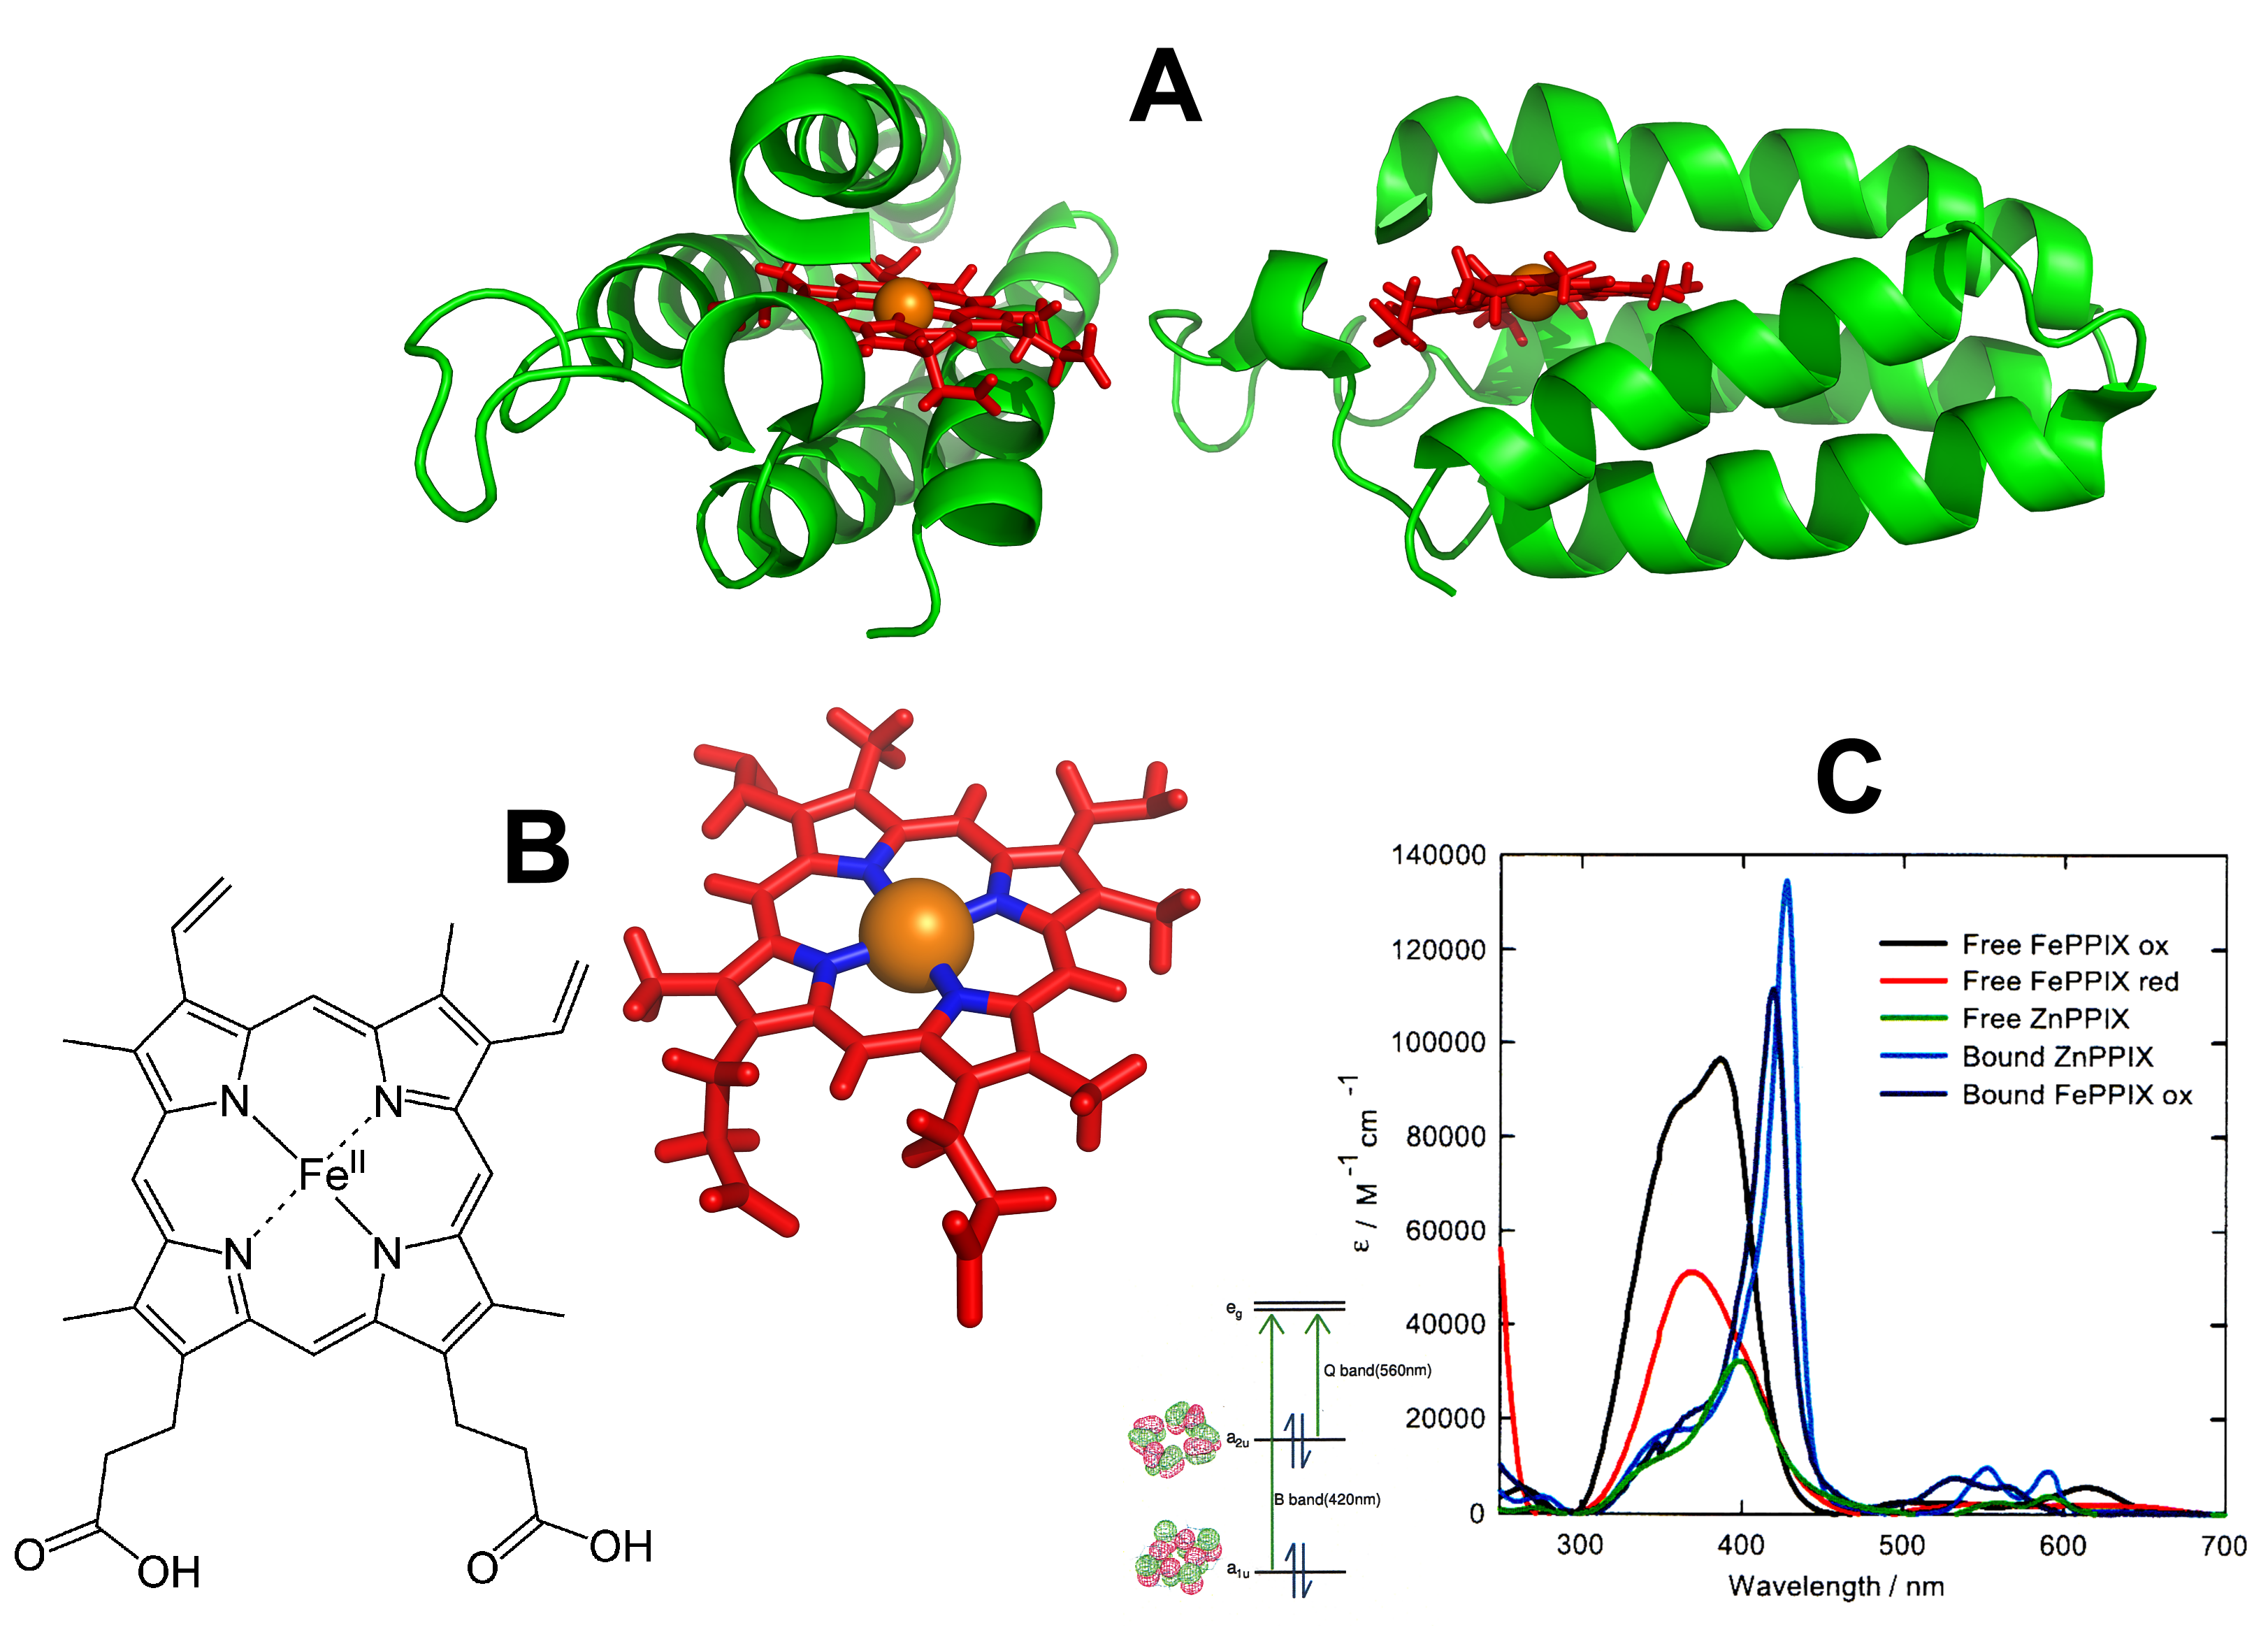
\includegraphics[width=137.4mm]{Images/haemStructure.png}
	\caption[Haem Structure]{A fancy image.}
	\label{fig:haemStructure}
\end{figure}
\end{verbatim}

\vspace{2ex}

\begin{figure}[!th]
	\centering
	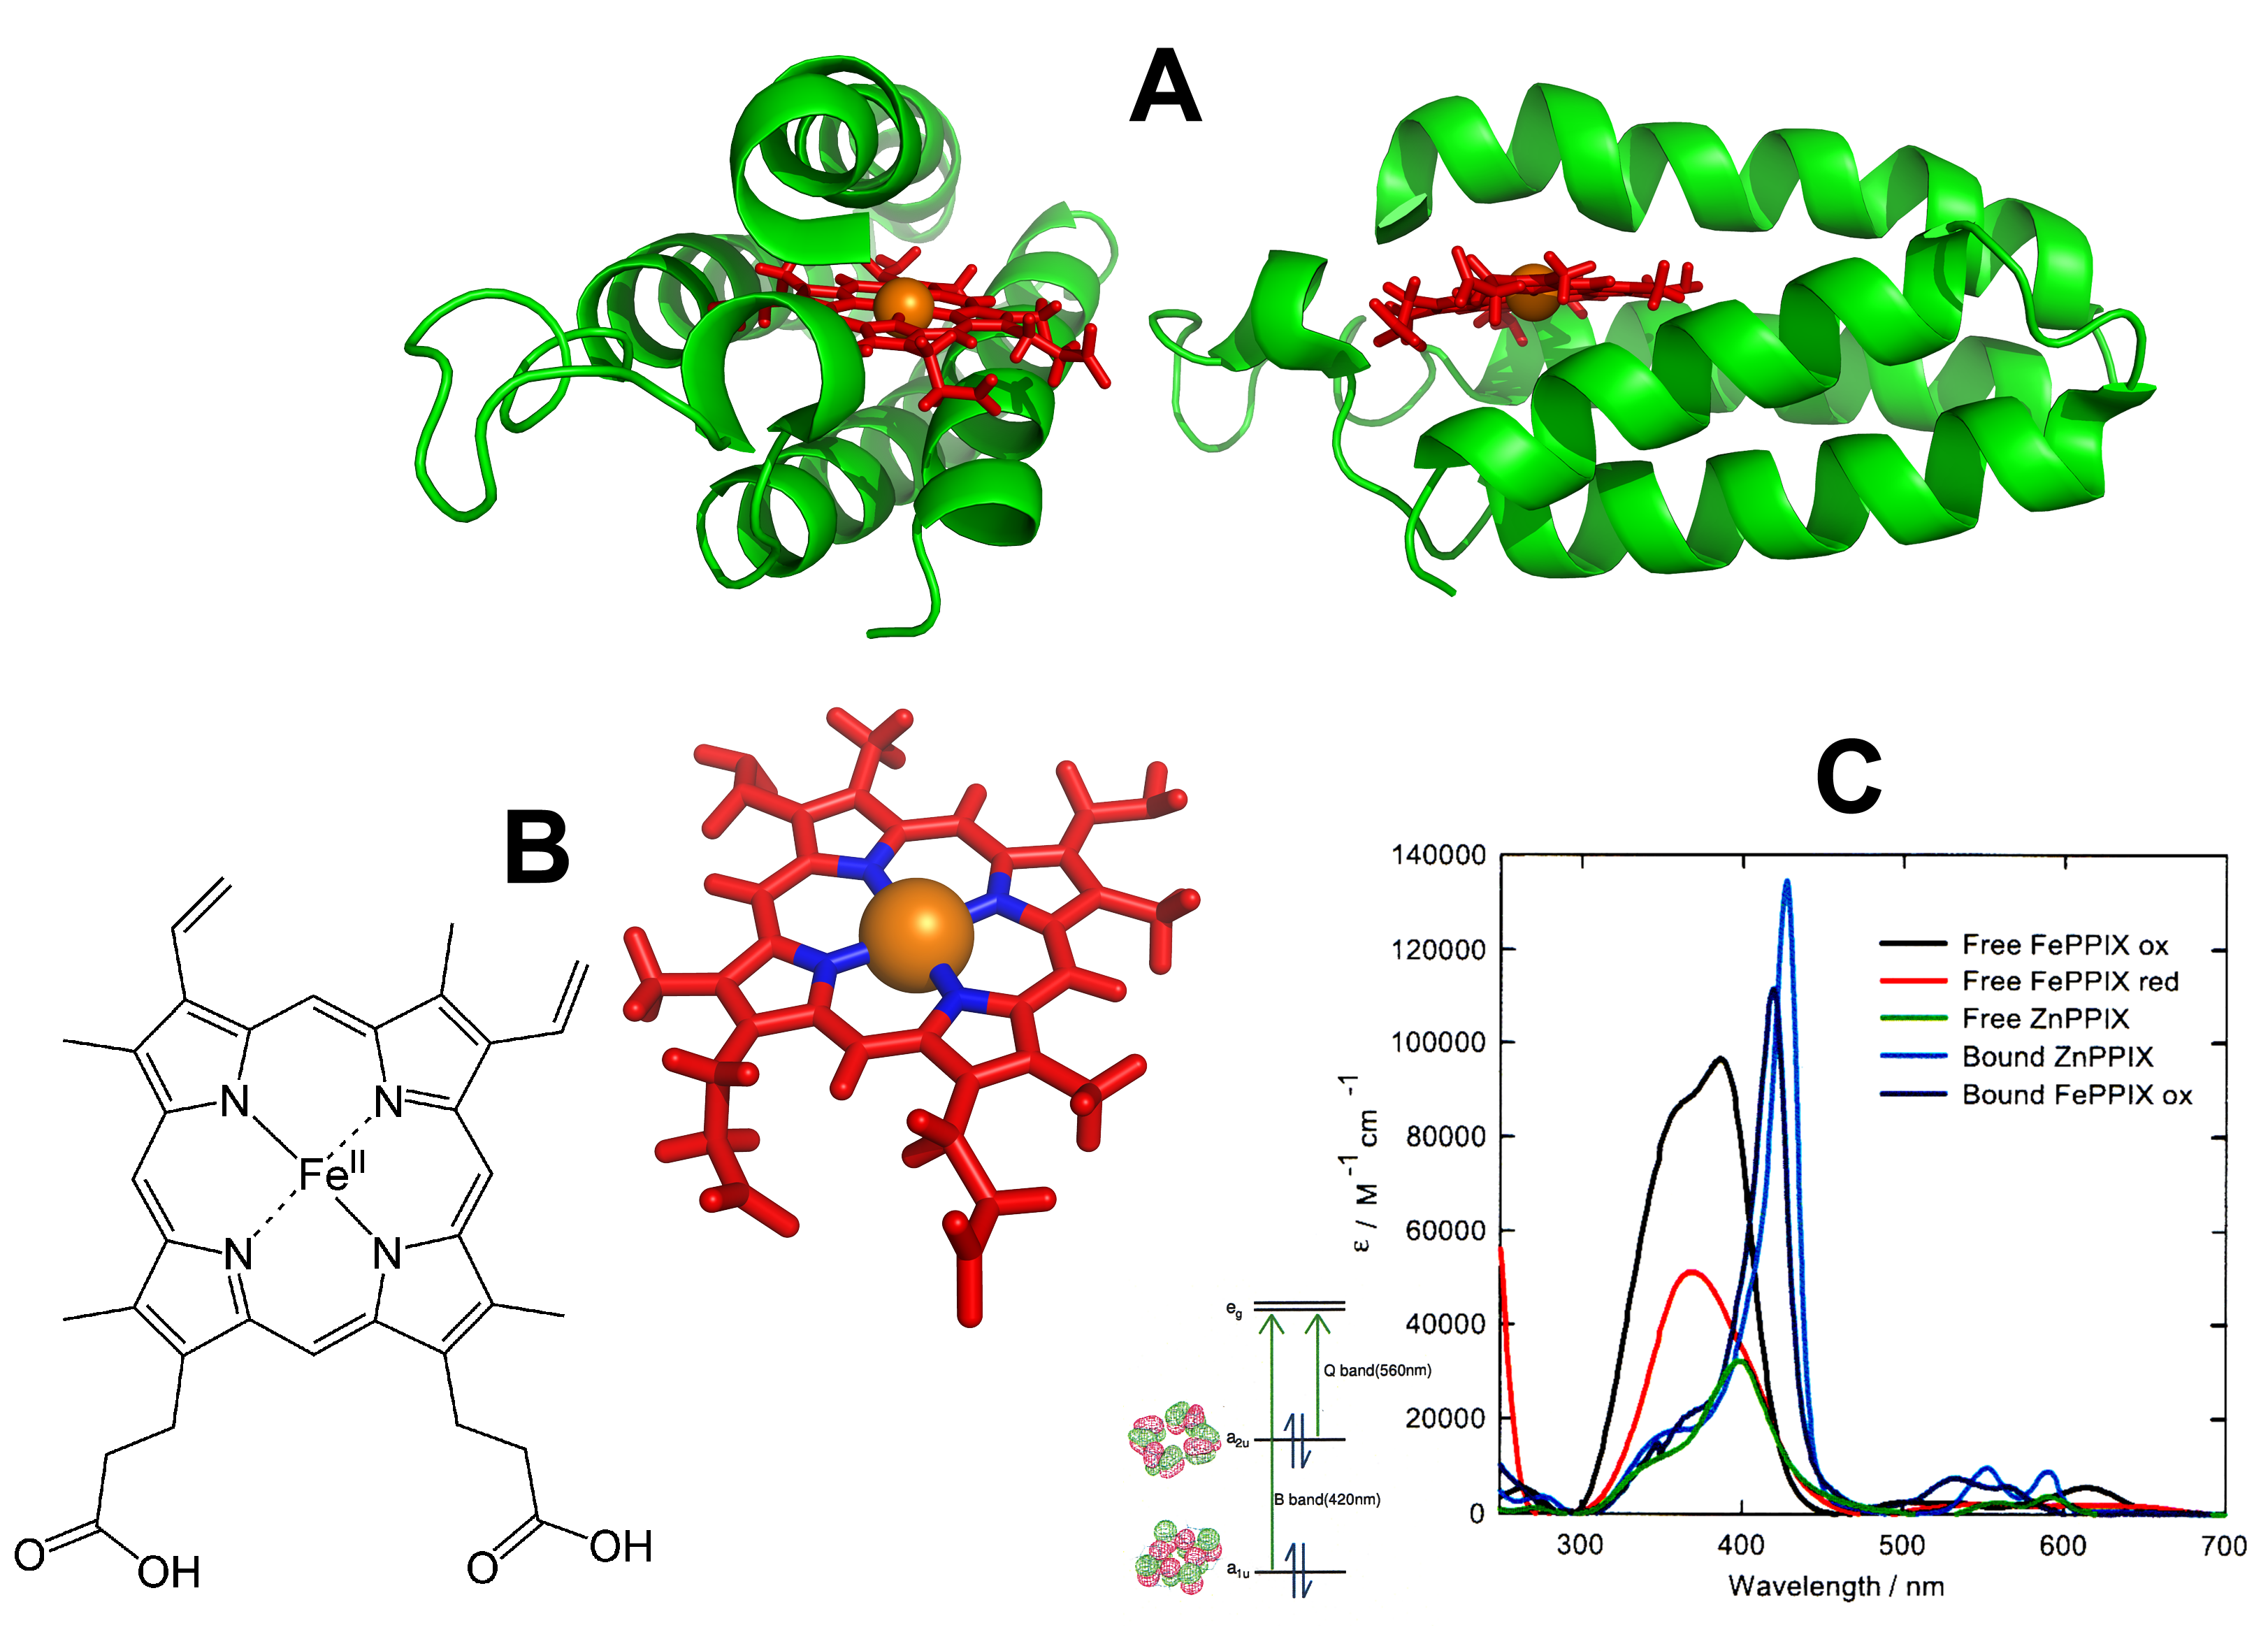
\includegraphics[width=137.4mm]{Images/haemStructure.png}
	\caption[Haem Structure]{A fancy image from Chris' Thesis.}
	\label{fig:haemStructure}
\end{figure}

In this example the command {\textbackslash}includegraphics tells LaTeX to look in the directory `Images' and incorporate the file called `haemStructure.png' into the final document while setting the width to 137.4mm.  This command can be used to resize a graphical file using the height or width parameter as shown. You must specify the units which can be pt, ex, em, mm, cm and so on. LaTeX recognises a very wide variety of standard units and graphics formats. The command is part of the graphicx package and so in the preamble you must include the command {\textbackslash}usepackage\{graphicx\}.

Many packages have been written to provide new commands. For example the `subfigure' package enables you to place separate images or files in the same figure side by side while giving them their own label. However, in this document we only concentrate on the very basics.

\section{Floating Environments}

Both tables and figures are examples of a `floating environments' which means LaTeX decides where to put them. 

The mysterious [!tbh] letters give guidance to LaTeX about roughly where the figure or table is  allowed to be, but in general they can move a long way from where you position them within your text file.  The letters in the square bracket can be t, h or b which stand for top, here or bottom.  If you don't specify any letters LaTeX defaults to [t].

LaTeX will always preserve the order in which figures appear.  If it cannot find a type setting solution, then it may move the float to it's own page, and combine it with other figures. If it still can't fit that in for some reason then it moves the float to the end of the document.  This has the effect of pushing all the remaining floating environments to the end of the document also.

The exclamation mark instructs LaTeX to ``try harder'' at putting the float where you told it to. Often you must play around to ensure the float positioning is acceptable, but usually this can be achieved by stretching or shrinking the image slightly using the size parameter, re-ordering text, judicial applications of the {\textbackslash}pagebreak command or by shouting loudly and slapping the computer monitor about. Note that it is better to resize the image using the original program that was used to create the image. Also using vector graphics can assist be useful (e.g. eps files) because they are designed to scale better.
\chapter{The Chapter on Making Chapters}
\label{sec:Chapters}

Right. LaTeX forces you to structure your document. There a series of simple commands for achieving this:

\vspace*{2ex}

{\textbackslash}chapter\{chapterName\}

{\textbackslash}section\{sectionName\}

{\textbackslash}subsection\{subsectionName\}

{\textbackslash}subsubsection\{subsubsectionName\}

\vspace*{2ex}

Easy enough. At the start of each chapter or section just issue one of these commands to name the section and LaTeX will present the chapter heading in the right style of font, which will be the same style of all the other heading names at that level of hierarchy throughout the document. In addition LaTeX assigns a number to that section. For example, this chapter was created using the command:

\vspace*{2ex}

{\textbackslash}chapter\{The Chapter on Making Chapters\} 

\vspace*{2ex}

LaTeX assigns the correct chapter number to each chapter in turn and then puts it in the table of contents, as you can see by looking at the table of contents! Easy.

\pagebreak
\section{The Section About Sections}
\label{sec:Section}
I think you're getting the hang of this. This section was created using the command {\textbackslash}section\{The Section About Sections\}. It appears in the table of contents as section \ref{sec:Section}.

\subsection{The Sub-Section About Sub-Sections}
\label{sec:SubSection}
Now you're really getting the hang of this. This subsection was created using the command {\textbackslash}subsection\{The Sub-Section About Sub-Sections\}. 

\subsubsection{The Sub-Sub-Section About Sub-Sub-Sections}
\label{sec:SubSubSection}
Now you're really getting the hang of this. but.. caught you out! This subsubsection doesn't have a number!  Ha Ha! It was created using the command {\textbackslash}subsubsection\{The Sub-Sub-Section About Sub-Sub-Sections\} in the same vein as all the other subsections/chapters etc. Here we have stopped the depth of the section numbering at the second level with the command:

\vspace*{2ex}

{\textbackslash}setcounter\{secnumdepth\}\{2\}

\vspace*{2ex}

Easy. WYSIWYM.  LaTeX does what you tell it to do. This is both a blessing and a curse.

\pagebreak
\section*{The Section About Sections That Don't Appear in the Table of Contents}
\label{sec:InvisibleSection}
Ok. Now we're throwing a spanner in the works. This section was created using the command:

\vspace*{2ex}

{\textbackslash}section*\{The Section About Sections That Don't Appear in the Table of Contents\}. 

\vspace*{2ex}

Notice how LaTeX has not assigned a number to the section and it doesn't appear in the table of contents. The effect of the * is to suppress the inclusion of a chapter, section or subsection in the automatic numbering. Easy. You can do this at any level. This is useful for things like prefaces, tables of contents or acknowledgements which you may or may not wish to have an entry in the main contents table. Up to you. It's your thesis. Don't just copy me.

\section{A Small Point About Numbering}

In this section notice how the numbering starts from where it left off before we suppressed the numbering on the previous section. Easy. WYSIWYM.
\pagebreak
\section{The Section About Internal Referencing}
\label{sec:InternalReferencing}

There are two related commands:

\vspace*{2ex}

{\textbackslash}label\{labelName\} 

{\textbackslash}ref\{labelName\}

\vspace*{2ex}


The {\textbackslash}label\{\} command allows you to create a label in a particular environment\footnote{That's right. Chapters, Sections and sub-sections etc are environments!}. The label won't appear in the final document. It's just a label which makes it easy to refer back to any particular environment elsewhere in the document. The {\textbackslash}ref\{\} command enables you to insert a reference anywhere in the document to any label in the document.  For example this is section \ref{sec:InternalReferencing}. The names you use in a label can be anything you like but musn't contain whitespace or special characters. I used the two commands:

\vspace*{2ex}

{\textbackslash}label\{sec:InternalReferencing\}

{\textbackslash}ref\{sec:InternalReferencing\}.

\vspace*{2ex}

The astute among you will realise that LaTeX has to read the document several times. Once to find the labels and then again to populate the references with the correct numbers. So you have to compile a latex document twice to get the referencing right. If there is a missing label or you refer to something that doesn't exist then latex inserts a convenient ? at that point. So hunting for queries is useful way of finding broken references. Latex issues warnings when it finds broken references.

As you create a document you will find yourself putting labels in all over the place so choose a sensible naming convention to help you remember the label names.

Each type of environment (equations, figures, tables, sections etc) has its own independent numbering system.  So when you choose your label name it's a good idea to have an identifier for that type of environment.  I have my own convention for label names which I use to help me remember references. E.g.   sec:SectionAboutCats. Eqn:EquationAboutCats,  Fig:FigureAboutCats and so on. This means you can differentiate between referring to the section or the figure more easily, even though they are about the same thing.

So Internal Referencing is a doddle. Easy!
\chapter{External Referencing}

Referencing is usually performed using a separate program called BibTex.  This program understands the file format .bib.

To create a reference within your document first you must create a .bib file by exporting your list of references from which ever referencing software you used, such as endnote, mendeley or whatever you use.

You can refer to an entry in the .bib file using the {\textbackslash}cite\{ref:Name\} command. the identifier `ref:Name' is the unique identifier which is the first line of each item included in your bibliography file.

For example, open the file LaTexCourseBib.bib in the bibliography directory. The first entry has the identifier `Horcas2007'.  This can be invoked as follows:


\begin{verbatim}
For example, this interesting fact\cite{Horcas2007}, is a cracking example.
\end{verbatim}

For example, this interesting fact\cite{Horcas2007}, is a cracking example.

During compilation latex and bibtex co-operate. During the first compilation latex generates a list of references that it needs.  During the second compilation bibtex populates the details from the .bib file into a shorter, ordered .bib file. The third compilation inserts markers at the right place in the main file and the fourth compilation generates the final list of references. Thus the compilation sequence is latex, bibtex, latex, latex.

The style of the referencing format can be changed using the command {\textbackslash}bibliographyStyle\{\}. e.g. the style used in this document is cjfthesisv1.bst which is invoked by 

\begin{verbatim}
\bibliographystyle{Bibliography/cjfthesisv1}
\end{verbatim}

The location of the list of references in the document is specified by issuing the {\textbackslash}bibliography\{\} command which also specifies the master bibliography file.

\begin{verbatim}
\bibliography{Bibliography/LaTeXCourseBib}
\end{verbatim}




\chapter{Organising Your Files}
One of the drawbacks of word is that the figures and tables are included within the document which becomes very very clunky quite quickly and once it reaches around 100Mb it becomes unwieldy and hard to export. One of that advantages of LaTeX is that the files are all text files and so are very light on resources and are easy to email around the place.

However, sometimes it can be difficult to navigate through a single text file, so if you had a huge document then it becomes difficult to find your way around.  One way of circumnavigating this problem is to break the file up into smaller files. As long as LaTeX knows where to look you can have a file for each logical sub-division of your document.

Therefore it is worth spending a bit of time at the beginning of a large project deciding how you wish to break up your LaTex Files and organise them neatly and tidily.  You can then tell LaTex where to look for the files using the following command:

\vspace*{2ex}
{\textbackslash}include\{fileName\}
\vspace*{2ex}

\pagebreak
\section{Linking a File}
We are now going to copy part of the tutorial file into a separate files and link it the main file.  Because this could go wrong it is sensible to back up tutorial.tex as something else. So save a copy called `tutorialOriginal.tex' for safe keeping. Then follow the following instructions.

\begin{enumerate}
\item Create a new file called MyFirstPage.tex
\item Select and Cut out the first chapter of Tutorial.Tex
\item Paste the first chapter into MyFirstPage.tex
\item Save both tutorial.tex and MyFirstPage.tex
\item Then add {\textbackslash}include\{MyFirstPage\} in tutorial.tex where the text used to be before you cut it out. We don't need to add the `.tex' because LaTeX can only include `.tex' files.
\item compile tutorial.tex and view the PDF
\end{enumerate}

The final PDF should look exactly the same as it was! except we now have a separate file for one of the chapters.

\pagebreak
\section{Creating A Class File}
We can also save our preamble in a separate file called a class file. This makes your main document much easier to understand.  To make it work we need to use the {\textbackslash}LoadClass\{\} command as follows: 

\begin{enumerate}
\item Create another new file and save it as TutorialStyle.cls
\item Copy the preamble of tutorial.tex into the new file. Starting with the {\textbackslash}documentclass{} command and copy right up to, but not including, the {\textbackslash}begin{document} command. Delete the preamble in the original document.
\item Save TutorialStyle.cls and tutorial.tex
\item Modify the first line of TutorialStyle.cls by replacing the word `document' with the word `Load'.
\item Add a new first line of tutorial.tex to use your new style class {\textbackslash}documentclass\{TutorialStyle\}
\item Save both files.
\end{enumerate}

\subsection{Sanity Check}

The first line of TutorialStyle.cls should now be:

\begin{verbatim}
\LoadClass[12pt, oneside, a4paper]{book}
\end{verbatim}
\vspace{2ex}

The first line of tutorial.tex should be:

\begin{verbatim}
\documentClass{TutorialStyle}
\end{verbatim}
\vspace{2ex}

We have just created what is called a style file. You can use this style file as a generic preamble for other documents as well. Compile tutorial.tex.  Nothing should have changed in the final PDF.


\pagebreak
\section{The Structure of this Document}

Lets now look at how I've organised this document. It is identical to my thesis because it started out life as my thesis. I usurped the structure and simply replaced the headings and content to make a kind of reference manual for this introductory course. This document therefore is three things:

\begin{enumerate}
\item An example thesis structure to work from.
\item The LaTeX files which were used to create it can be used as a template for a thesis.
\item It is also a convenient introductory latex manual!
\end{enumerate}

\vspace*{2ex}
Groovy huh?

\section{The Master File}

There is a master file where LaTeX begins the compilation procedure. This contains the {\textbackslash}documentclass command needed to set the ball rolling. Within the file there are a series of {\textbackslash}include\{\} commands, one for each Chapter, which tell LaTeX where to find the files containing each chapter.

The subfiles cannot be compiled on their own because they do not contain the {\textbackslash}documentclass, {\textbackslash}begin\{document\} or {\textbackslash}end\{document\} commands. Lets us look in more detail at the master file and we will learn some new LaTeX commands.

\singlespacing
\pagebreak
\begin{verbatim}
\documentclass{Style/LatexCourseStyle}

\begin{document}
\setcounter{secnumdepth}{2}
\setcounter{tocdepth}{1}

\frontmatter
\onehalfspacing
\include{Frontmatter/Titlepage}
\include{Frontmatter/Declaration}
\include{Frontmatter/Acknowledgements}
\include{Frontmatter/Summary}
\include{Frontmatter/Abbreviations}
\tableofcontents
\listoftables
\listoffigures

\mainmatter
\renewcommand{\sectionmark}[1]{\markright{\thesection \ #1}{}}
\include{Chapters/Overview}
\include{Chapters/MyFirstPage}
\include{Chapters/Lists}
\include{Chapters/mathsEquations}
\include{Chapters/ChemicalEquations}
\include{Chapters/Tables}
\include{Chapters/Figures}
\include{Chapters/Sectioning}
\include{Chapters/externalReferencing}
\include{Chapters/ThesisTemplateMainFile}
%\include{Chapters/ChapterThatIsNotCompiled}

\appendix
%\include{Appendices/UsefulWebsites}

\singlespacing

\backmatter
\addcontentsline{toc}{chapter}{References}
\bibliographystyle{Bibliography/cjfthesisv1}
\renewcommand{\bibname}{References}
\bibliography{Bibliography/LatexCourseBib}

\end{document}
\end{verbatim}
\onehalfspacing
\pagebreak

\section{Analysing the Master File}
Let us go through this file and observe the new commands. Most of it is self-explanatory.

\begin{verbatim}
\documentclass{Style/LaTeXCourseStyle}
\end{verbatim}

This command tells latex that the document class is the one defined in the the style file ''LaTeXCourseStyle'', which is in the sub directory ''style''.  Easy.

\begin{verbatim}
\setcounter{secnumdepth}{2}
\setcounter{tocdepth}{1}
\end{verbatim}

The first of these commands tells latex that the section depth number is 2. I.E. throughout the document only bother numbering sections, subsections and subsubsections down to the second level (such as section 1.2.3). The second command tells latex to only build the table of contents from section numbers down to the first level i.e. 1.1.  Easy enough.

The command {\textbackslash}frontmatter is exclusive to the book class, on which this style is based, and tells latex that within this section to number the pages using roman numerals, and not to include these numbers in the table of contents, just like in a book. The {\textbackslash}mainmatter and {\textbackslash}backmatter commands similarly delineate the other sections of the document.  

Childs play.  How long would it take you to figure out how to do that in word???? No idea. I've never tried.

Note that these rather cool commands are not available in every single class. So for a paper you would use the article class where such compartmentalisation of your document is not appropriate. In fact you can often download latex templates from the journal to wish to submit your paper, which is why I concentrate on the thesis template in this course.

\begin{verbatim}
\onehalfspacing
\end{verbatim}

Is obvious. ''From this point forward use line spacing of one and a half lines please. Thank you.'' How many hours have you spent clicking on paragraph indentations for each separate paragraphs in word? Nightmare. Want to change the standard in the whole document? Not a chance in word. In latex, you can do it with a single word, carefully placed in the master file.

\begin{verbatim}
\include{Frontmatter/Titlepage}
\include{Frontmatter/Declaration}
\include{Frontmatter/Acknowledgements}
\include{Frontmatter/Summary}
\include{Frontmatter/Abbreviations}
\end{verbatim}

The {\textbackslash}include\{\} command tells latex to include the specified .tex file at this point.  Thus it is a simple matter to break up a large document into sub components.  I have written each part of the front matter in a separate file and then grouped all the front matter into one directory called: Frontmatter.

See how the directory structure of my files reflects the structure of my book?

\begin{verbatim}
\tableofcontents
\listoftables
\listoffigures
\end{verbatim}

Again. This is easy. These commands mean: ''Please scan through the whole document and build for me a table of contents, a list of tables, a list of figures and then write down the entries along side their section numbers (as I have them ordered in this version of the document), as well as the page numbers on which they appear and create a nice little summary table and add them to the front matter of my document. Thanks.''.

How does latex do this?  remember the idea of environments?  Well each table, figure, equation etc is a defined environment.  LaTeX just counts them up and assigns numbers starting wherever you want and builds a table.  You can tell latex to ignore individual sections if you want to.

You can also control the look and feel of your table of contents with subtley and grace. Do you want to fill the white space with lines of dots to aid readability, even though the chapter titles are all different lengths? page numbers? How deep should the TOC been?  etc etc etc. How to do this is beyond the scope of this course, but now you know about it, go look it up. easy as $\pi$.

Ok.

Main matter we've done.

\begin{verbatim}
\renewcommand{\sectionmark}[1]{\markright{\thesection \ #1}{}}
\end{verbatim}

This command tells latex to 'renewcommand', i.e. change the meaning of the following command from this point in the document forward, over-riding previous definitions.
\begin{verbatim}
\sectionmark}[1]{\markright{\thesection \ #1}{}
\end{verbatim}

Is latex speak for ``please write the section heading at the top right hand side of each page. thanks''. This works in conjunction with a command in the style file which we'll talk about later. You have to tell latex to switch on headings as well as where to put them.

\begin{verbatim}
\include{Chapters/Overview}
\include{Chapters/MyFirstPage}
\include{Chapters/Lists}
\include{Chapters/mathsEquations}
\include{Chapters/ChemicalEquations}
\include{Chapters/Tables}
\include{Chapters/Figures}
\include{Chapters/Sectioning}
\include{Chapters/externalReferencing}
\include{Chapters/ThesisTemplateMainFile}
%\include{Chapters/ChapterThatIsNotCompiled}
\end{verbatim}

This is the include command again. You will notice that one of the include lines is commented out. This is a handy trick to only build certain parts of my thesis. Which can be useful if individual chapters are being reviewed.

\pagebreak

\begin{verbatim}
\appendix
%\include{Appendices/UsefulWebsites}

\singlespacing

\backmatter
\addcontentsline{toc}{chapter}{References}
\bibliographystyle{Bibliography/cjfthesisv1}
\renewcommand{\bibname}{References}
\bibliography{Bibliography/LatexCourseBib}
\end{verbatim}

The rest is easy. {\textbackslash}Appendix means we are in the appendix now and start labelling sections with A.1.2 instead of 1.2.3.  

{\textbackslash}addcontentsline means forcibly insert a contents line about the references into the contents table. 

{\textbackslash}\{bibliographystyle\{Bibliography/cjfthesisv1\}\} means use the biblography style defined in the file cjfthesisv1. Defining a bibliography style will be covered later if we have time. This is where you specify how the references will appear (names, journals, full stops, commas etc).

{\textbackslash}renewcommand\{{\textbackslash}bibname\}\{References\} means: rename the bibliography chapter as `References'

{\textbackslash}biblography means add the following bibliography.  You can reference entries in this bibliography file very easily.

The astute among you will realise that LaTeX will have to read the document several times before it can be compiled with all the references.  Hey ho. No problem. You can go and have a cuppa while LaTeX does your references for you in the style of your favorite journal... nice.




%\include{Chapters/ChapterThatIsNotCompiled}
\end{verbatim}

This is the include command again. You will notice that one of the include lines is commented out. This is a handy trick to only build certain parts of my thesis. Which can be useful if individual chapters are being reviewed.

\pagebreak

\begin{verbatim}
\appendix
%\include{Appendices/UsefulWebsites}

\singlespacing

\backmatter
\addcontentsline{toc}{chapter}{References}
\bibliographystyle{Bibliography/cjfthesisv1}
\renewcommand{\bibname}{References}
\bibliography{Bibliography/LatexCourseBib}
\end{verbatim}

The rest is easy. {\textbackslash}Appendix means we are in the appendix now and start labelling sections with A.1.2 instead of 1.2.3.  

{\textbackslash}addcontentsline means forcibly insert a contents line about the references into the contents table. 

{\textbackslash}\{bibliographystyle\{Bibliography/cjfthesisv1\}\} means use the biblography style defined in the file cjfthesisv1. Defining a bibliography style will be covered later if we have time. This is where you specify how the references will appear (names, journals, full stops, commas etc).

{\textbackslash}renewcommand\{{\textbackslash}bibname\}\{References\} means: rename the bibliography chapter as `References'

{\textbackslash}biblography means add the following bibliography.  You can reference entries in this bibliography file very easily.

The astute among you will realise that LaTeX will have to read the document several times before it can be compiled with all the references.  Hey ho. No problem. You can go and have a cuppa while LaTeX does your references for you in the style of your favorite journal... nice.




%\include{Chapters/ChapterThatIsNotCompiled}
\end{verbatim}

This is the include command again. You will notice that one of the include lines is commented out. This is a handy trick to only build certain parts of my thesis. Which can be useful if individual chapters are being reviewed.

\pagebreak

\begin{verbatim}
\appendix
%\include{Appendices/UsefulWebsites}

\singlespacing

\backmatter
\addcontentsline{toc}{chapter}{References}
\bibliographystyle{Bibliography/cjfthesisv1}
\renewcommand{\bibname}{References}
\bibliography{Bibliography/LatexCourseBib}
\end{verbatim}

The rest is easy. {\textbackslash}Appendix means we are in the appendix now and start labelling sections with A.1.2 instead of 1.2.3.  

{\textbackslash}addcontentsline means forcibly insert a contents line about the references into the contents table. 

{\textbackslash}\{bibliographystyle\{Bibliography/cjfthesisv1\}\} means use the biblography style defined in the file cjfthesisv1. Defining a bibliography style will be covered later if we have time. This is where you specify how the references will appear (names, journals, full stops, commas etc).

{\textbackslash}renewcommand\{{\textbackslash}bibname\}\{References\} means: rename the bibliography chapter as `References'

{\textbackslash}biblography means add the following bibliography.  You can reference entries in this bibliography file very easily.

The astute among you will realise that LaTeX will have to read the document several times before it can be compiled with all the references.  Hey ho. No problem. You can go and have a cuppa while LaTeX does your references for you in the style of your favorite journal... nice.




\chapter{The Chapter on Making Chapters}
\label{sec:Chapters}

Right. LaTeX forces you to structure your document. There a series of simple commands for achieving this:

\vspace*{2ex}

{\textbackslash}chapter\{chapterName\}

{\textbackslash}section\{sectionName\}

{\textbackslash}subsection\{subsectionName\}

{\textbackslash}subsubsection\{subsubsectionName\}

\vspace*{2ex}

Easy enough. At the start of each chapter or section just issue one of these commands to name the section and LaTeX will present the chapter heading in the right style of font, which will be the same style of all the other heading names at that level of hierarchy throughout the document. In addition LaTeX assigns a number to that section. For example, this chapter was created using the command:

\vspace*{2ex}

{\textbackslash}chapter\{The Chapter on Making Chapters\} 

\vspace*{2ex}

LaTeX assigns the correct chapter number to each chapter in turn and then puts it in the table of contents, as you can see by looking at the table of contents! Easy.

\pagebreak
\section{The Section About Sections}
\label{sec:Section}
I think you're getting the hang of this. This section was created using the command {\textbackslash}section\{The Section About Sections\}. It appears in the table of contents as section \ref{sec:Section}.

\subsection{The Sub-Section About Sub-Sections}
\label{sec:SubSection}
Now you're really getting the hang of this. This subsection was created using the command {\textbackslash}subsection\{The Sub-Section About Sub-Sections\}. 

\subsubsection{The Sub-Sub-Section About Sub-Sub-Sections}
\label{sec:SubSubSection}
Now you're really getting the hang of this. but.. caught you out! This subsubsection doesn't have a number!  Ha Ha! It was created using the command {\textbackslash}subsubsection\{The Sub-Sub-Section About Sub-Sub-Sections\} in the same vein as all the other subsections/chapters etc. Here we have stopped the depth of the section numbering at the second level with the command:

\vspace*{2ex}

{\textbackslash}setcounter\{secnumdepth\}\{2\}

\vspace*{2ex}

Easy. WYSIWYM.  LaTeX does what you tell it to do. This is both a blessing and a curse.

\pagebreak
\section*{The Section About Sections That Don't Appear in the Table of Contents}
\label{sec:InvisibleSection}
Ok. Now we're throwing a spanner in the works. This section was created using the command:

\vspace*{2ex}

{\textbackslash}section*\{The Section About Sections That Don't Appear in the Table of Contents\}. 

\vspace*{2ex}

Notice how LaTeX has not assigned a number to the section and it doesn't appear in the table of contents. The effect of the * is to suppress the inclusion of a chapter, section or subsection in the automatic numbering. Easy. You can do this at any level. This is useful for things like prefaces, tables of contents or acknowledgements which you may or may not wish to have an entry in the main contents table. Up to you. It's your thesis. Don't just copy me.

\section{A Small Point About Numbering}

In this section notice how the numbering starts from where it left off before we suppressed the numbering on the previous section. Easy. WYSIWYM.
\pagebreak
\section{The Section About Internal Referencing}
\label{sec:InternalReferencing}

There are two related commands:

\vspace*{2ex}

{\textbackslash}label\{labelName\} 

{\textbackslash}ref\{labelName\}

\vspace*{2ex}


The {\textbackslash}label\{\} command allows you to create a label in a particular environment\footnote{That's right. Chapters, Sections and sub-sections etc are environments!}. The label won't appear in the final document. It's just a label which makes it easy to refer back to any particular environment elsewhere in the document. The {\textbackslash}ref\{\} command enables you to insert a reference anywhere in the document to any label in the document.  For example this is section \ref{sec:InternalReferencing}. The names you use in a label can be anything you like but musn't contain whitespace or special characters. I used the two commands:

\vspace*{2ex}

{\textbackslash}label\{sec:InternalReferencing\}

{\textbackslash}ref\{sec:InternalReferencing\}.

\vspace*{2ex}

The astute among you will realise that LaTeX has to read the document several times. Once to find the labels and then again to populate the references with the correct numbers. So you have to compile a latex document twice to get the referencing right. If there is a missing label or you refer to something that doesn't exist then latex inserts a convenient ? at that point. So hunting for queries is useful way of finding broken references. Latex issues warnings when it finds broken references.

As you create a document you will find yourself putting labels in all over the place so choose a sensible naming convention to help you remember the label names.

Each type of environment (equations, figures, tables, sections etc) has its own independent numbering system.  So when you choose your label name it's a good idea to have an identifier for that type of environment.  I have my own convention for label names which I use to help me remember references. E.g.   sec:SectionAboutCats. Eqn:EquationAboutCats,  Fig:FigureAboutCats and so on. This means you can differentiate between referring to the section or the figure more easily, even though they are about the same thing.

So Internal Referencing is a doddle. Easy!
%\include{Chapters/User Defined Commands}
%\include{Chapters/External Referencing}
\end{verbatim}

This is the include command again. You will notice that some of the include lines are commented out. This is because I haven't written those files yet, if I tried to compile and the file wasn't there then latex would politely inform me that it was unable to find the file. In general I can comment out lines in the main file to suppress their inclusion in a shorter version of my thesis. Say I wish to build just one chapter, all I need to do is put \% signs everywhere except the chapter that I want to include. This will recreate the table of contents with only the chapters that are included.

\pagebreak

\begin{verbatim}
\appendix
%\include{Appendices/UsefulWebsites}

\singlespacing

\backmatter
%\addcontentsline{toc}{chapter}{References}
%\bibliographystyle{Bibliography/cjfthesisv1}
%\renewcommand{\bibname}{References}
%\bibliography{Bibliography/LaTeXCourseBib}
\end{verbatim}

Finally the rest is easy. {\textbackslash}Appendix means we are in the appendix now and start labelling sections with A.1.2 instead of 1.2.3.  

{\textbackslash}addcontentsline means forcibly insert a contents line about the references into the contents table. 

{\textbackslash}\{bibliographystyle\{Bibliography/cjfthesisv1\}\} means use the biblography style defined in the file cjfthesisv1. Defining a bibliography style will be covered later if we have time. This is where you specify how the references will appear (names, journals, full stops, commas etc).

{\textbackslash}biblography means add the following bibliography.  You can reference entries in this bibliography file very easily.

The astute among you will realise that LaTeX will have to read the document several times before it can be compiled with all the references.  Hey ho. No problem. You can go and have a cuppa while LaTeX does your references for you in the style of your favorite journal... nice.

\pagebreak
\section{Creating A Class File}
You can also use the {\textbackslash}LoadClass\{\} command to allow your preamble to be saved in a separate file. This makes your main document much easier to understand.

\begin{enumerate}
\item Create another new file and save it as TutorialStyle.cls
\item Copy the preamble of tutorial.tex into the new file. Starting with the {\textbackslash}documentclass{} command and copy right up to, but not including, the {\textbackslash}begin{document} command. Delete the preamble in the original document.
\item Save TutorialStyle.cls and tutorial.tex
\item Modify the first line of TutorialStyle.cls by replacing the word `document' with the word `Load'.
\item Modify the first line of tutorial.tex to become {\textbackslash}documentclass\{TutorialStyle\}
\item Save both files.
\end{enumerate}

\subsection{Sanity Check}

The first line of TutorialStyle.cls should now be:

\begin{verbatim}
\LoadClass[12pt, oneside, a4paper]{book}
\end{verbatim}
\vspace{2ex}

The first line of tutorial.tex should be:

\begin{verbatim}
\documentClass{TutorialStyle}
\end{verbatim}
\vspace{2ex}

We have just created what is called a style file. You can use this style file as a generic preamble for other documents as well. Compile tutorial.tex.  Nothing should have changed in the final PDF.




